\PassOptionsToPackage{no-math}{fontspec}
\documentclass[UTF8,zihao=5,openany,fontset=windows]{ctexbook}
\usepackage[paperwidth=210mm,paperheight=279mm,inner=25mm,outer=23mm,top=24mm,bottom=23mm,headheight=14pt]{geometry}
\usepackage{fontspec}
\setmainfont{Times New Roman}
\setsansfont{Arial}
\setmonofont{Consolas}[Scale=0.85]
\usepackage{amsmath,amssymb,mathtools}
\usepackage{newtxmath}
\DeclareSymbolFont{operators}{OT1}{ntxtlf}{m}{n}
\SetSymbolFont{operators}{bold}{OT1}{ntxtlf}{b}{n}
\DeclareMathAlphabet{\mathbf}{OT1}{ntxtlf}{b}{n}
\SetMathAlphabet{\mathbf}{bold}{OT1}{ntxtlf}{b}{n}
\DeclareMathAlphabet{\mathsf}{OT1}{cmss}{m}{n}
\SetMathAlphabet{\mathsf}{bold}{OT1}{cmss}{bx}{n}
\usepackage{booktabs,longtable,tabularx,array,multirow}
\usepackage{graphicx,xcolor,siunitx}
\usepackage{flafter}
\usepackage{enumitem,listings,fancyhdr}
\usepackage{xeCJK-listings}
\setCJKmonofont{NSimSun}
\usepackage[unicode,colorlinks=true,linkcolor=black,citecolor=black,urlcolor=blue!55!black,bookmarksnumbered=true]{hyperref}
\ctexset{chapter={format=\bfseries\zihao{3},beforeskip=22pt,afterskip=26pt},section={format=\bfseries\zihao{-4},beforeskip=16pt,afterskip=8pt},subsection={format=\bfseries\zihao{5},beforeskip=12pt,afterskip=6pt}}
\linespread{1.18}
\setlength{\parindent}{2em}
\setlength{\parskip}{2pt}
\setlength{\emergencystretch}{2em}
\setcounter{tocdepth}{1}
\numberwithin{equation}{chapter}
\allowdisplaybreaks[1]
\pagestyle{fancy}
\fancyhf{}
\fancyhead[LE,RO]{\small\thepage}
\fancyhead[RE]{\small\nouppercase{\leftmark}}
\fancyhead[LO]{\small\nouppercase{\rightmark}}
\renewcommand{\headrulewidth}{0.3pt}
\fancypagestyle{plain}{\fancyhf{}\fancyfoot[C]{\small\thepage}\renewcommand{\headrulewidth}{0pt}}
\setlist{nosep,leftmargin=2em}
\renewcommand{\arraystretch}{1.18}
\lstset{basicstyle=\ttfamily\fontsize{8.1}{10}\selectfont,numbers=left,numberstyle=\tiny\color{gray},numbersep=6pt,breaklines=true,breakatwhitespace=false,columns=fullflexible,keepspaces=true,showstringspaces=false,tabsize=4,keywordstyle=\color{blue!60!black},commentstyle=\color{black!60},stringstyle=\color{black!75},frame=none}

\begin{document}
\frontmatter
\begin{titlepage}\centering\vspace*{26mm}
{\bfseries\zihao{1}超图优化与异构无人集群巡检\par}\vspace{10mm}
{\zihao{3}数学建模、求解方法与评价\par}\vspace{18mm}
{\zihao{-4}教学专著\par}
\vfill{\small 理论模型、参数实例与实验结果\par}
\end{titlepage}
\tableofcontents
\mainmatter
\setcounter{chapter}{0}
\chapter{研究问题与建模层次}
\setcounter{section}{0}
\section{研究对象与决策问题}
\label{sec:01_01}

一项候选任务可能同时需要多种不可分资源，而其中任何一种资源也可能被其他任务需要。接受该任务，就意味着同时承诺它所要求的全部资源；若某项资源不能重复分配，这一选择便会排除其他需要该资源的候选。纯组合模型首先研究这种共同占用引起的选择限制。设$V$为有限资源集合，$E$为有限候选任务集合，每个候选任务$e\in E$以其所需资源的非空子集$e\subseteq V$表示，由此得到超图$H=(V,E)$：顶点表示资源，超边表示候选任务。对每个$e\in E$，无量纲二元变量$x_e\in\{0,1\}$表示是否接受任务，固定正权重$w_e\in\mathbb{R}_{>0}$表示统一评价尺度下的收益，本节将其视为无量纲分值；选择的目标是最大化总收益$\sum_{e\in E}w_ex_e$。资源$v\in V$的容量$b_v\in\mathbb{Z}_{\geq 0}$表示允许接受的占用份数，为无量纲计数。当前全部组合实验采用$b_v=1$，因此任意两个不同候选$e,f\in E$满足
\begin{equation}
 e\cap f\ne\varnothing,
 \quad x_e=1
 \quad\Longrightarrow\quad x_f=0.
 \label{s0101:shared_resource}
\end{equation}
这里的占用针对预先定义的候选及资源关系，不自动描述设备完成任务后如何释放、移动和再次使用。若同一设备可以在不同时段服务多个任务，就需要进一步描述占用时段和状态接续，不能把静态容量一解释为一台设备在整个班次内只能执行一次任务。

电力巡检将这种资源选择放入具体的空间与时间过程。巡检对象是杆塔及其需要观测的部位，执行资源包括车辆、无人机和具有独立身份的物理电池对。分别以有限集合$\mathcal{G}$、$\mathcal{V}$、$\mathcal{U}$和$\mathcal{B}$表示杆塔、车辆、无人机和物理电池对，其中车辆集合$\mathcal{V}$与组合模型的资源集合$V$区别使用；对每座杆塔$g\in\mathcal{G}$，以有限集合$\mathcal{I}_g$表示其必需观测项。车辆携带无人机与电池沿道路移动，无人机从满足条件的位置起飞，对杆塔不同部位实施观测，再与车辆会合回收；回收后的电池可以按其状态继续使用、换装或充电。因此，联合决策既要回答哪些观测交给哪架无人机，也要确定哪些观测组成同一航次、按什么顺序执行、由哪辆车支持、在哪里起飞和回收，以及使用哪一对电池。电池对具有实际位置、剩余能量和可用时刻，不能仅以一个可任意分配的总电量代替。

上述决定通过路径、事件时刻和资源状态相互影响。改变车辆停靠点，会改变无人机往返观测位置的距离，并影响车辆到达后续回收地点的时间；在同一航次中增加观测项，可能减少起降次数，也会改变飞行历时、耗电量与回收时刻；电池较晚返回车辆，则会推迟它开始充电或再次装机的时刻，进而限制后续航次。无人机到达杆塔附近也不等于完成观测：观测位置、姿态、可见性和成像质量须满足要求，连接这些观测状态的连续路径还须满足运动、障碍物避让、安全距离及能量条件。即使车辆路径和无人机路径分别可行，两者也可能因无法按时会合而不能共同执行。因此，任务分配必须与连续路径、观测状态、车辆移动、起降回收和电池周转一起决定。一个分配选择只有能够由相应的物理过程实现，才构成可执行的巡检安排。

巡检首先评价完整杆塔的完成数量，而不是累计拍摄次数。当前任务定义中，每座杆塔有九项必需观测，即对所有$g\in\mathcal{G}$均有$|\mathcal{I}_g|=9$；九项全部满足验收条件，才计为一座完整杆塔。缺少其中任何一项合格观测，该塔就不能计入完整完成数量，不同杆塔的零散观测也不能相互补足。用无量纲二元变量$z_g\in\{0,1\}$表示杆塔$g$在模型中的完整完成状态，其值为一当且仅当该塔全部必需观测均完成并满足模型规定的验收条件。相应的未完成杆塔数为
\begin{equation}
 N_{\mathrm{miss}}=\sum_{g\in\mathcal{G}}(1-z_g),
 \qquad
 N_{\mathrm{miss}}\in\{0,1,\ldots,|\mathcal{G}|\}.
 \label{s0101:uncompleted_towers}
\end{equation}
该量以杆塔座数计，整塔状态与各项观测之间的正式线性约束在第5章建立。以未完成数量为目标，允许在资源和物理条件限制下出现部分完成，并未预先要求所有杆塔必须完成。这里的完成状态是模型对计划的判定；执行后的实际验收仍须依据获得的观测资料和执行记录确认，不能由计划中的$z_g=1$直接替代。

在完整杆塔数量之后，还需比较全队结束任务的时间和无人机的机载耗电。令$T_{\mathrm{return}}\in\mathbb{R}_{\geq 0}$表示从统一任务起点到全队完成必要回收并返库的历时，单位为$\mathrm{s}$；令$E_{\mathrm{air}}\in\mathbb{R}_{\geq 0}$表示本次规划计入的机载耗电量，单位为$\mathrm{Wh}$。对于给定信息与给定情形下的一次规划，在满足物理及资源条件的方案中采用词典序目标
\begin{equation}
 \operatorname{lexmin}
 \bigl(N_{\mathrm{miss}},\ T_{\mathrm{return}},\ E_{\mathrm{air}}\bigr).
 \label{s0101:lexicographic_objective}
\end{equation}
比较两个方案时，先选择未完成杆塔较少的方案；仅当未完成数量相同，才比较全队返库历时；仅当前两项均相同，才比较机载耗电量。因此，少完成一座完整杆塔不能由更早返库或更低耗电补偿。一般加权混合目标通过权重规定不同指标之间的交换比例，可能接受完成数量与时间、耗电之间的交换，且权重须处理不同量纲；词典序则直接规定比较顺序，不必将杆塔座数、秒和瓦时换算为一个共同分值。第三级目标仅累计当前规划时刻至各航次结束的机载功率积分，功率以$\mathrm{W}$、时间以$\mathrm{s}$计时须除以$3600$换算为$\mathrm{Wh}$，初次规划从任务起点计起，已发生的耗电作为常数，充电电网输入另行报告，车辆牵引耗能不计入该目标。上述说明明确一次规划中的优先关系，情形集合下的推广在后文讨论。

作出这些决定，需要区分已知条件、当前状态和未来信息。地理位置、道路与障碍物描述、观测要求、设备能力及服务规则构成建模输入；车辆与无人机的位置、电池的位置与剩余能量、已完成观测和正在执行的动作构成状态输入。真实地理参考仿真能够保留任务的空间联系，但其目标几何和部分设备、服务参数采用模板或参考值，并不等于现场实测。对于尚未发生的天气变化、行驶耗时、能量消耗及观测结果，规划须依据当时可得的参考值、预测值或明确给定的不确定性描述，不能把未来实际值当作当前已知信息。方案的模型可行性也相应取决于所用输入和假设。执行中获得新信息后，后续安排须接续实际状态：已经移动到的位置、已经消耗的能量和尚未结束的动作，不能因重新分配任务而被重置。信息更新因此既可能改变方案的评价值，也可能改变后续航次、会合与充电安排的可行性。

纯组合选择与巡检联合决策共同研究资源联系下的活动组织，但承担不同的数学任务。前者在预先给定的有限候选、固定收益和资源关联中选择任务；后者还须决定路径与时序，并连接位置、能量和观测等物理状态，其完整形式包含离散变量、连续变量及非线性关系。当前容量一的组合可行域可以用两两冲突表达，超边含有较多资源本身并不构成不可约高阶耦合或求解性能优势的证据。组合实验中的选择质量和求解行为，因而不能直接迁移为巡检方案的路径、能量或会合可行性结论。要描述联合可执行性，首先需要明确哪些活动关联哪些资源，以及这些关联分别限制什么选择；超图提供了组织这类关联的表示方式，其基本对象及组合含义由此成为后续建模的起点。

\setcounter{section}{1}
\section{超图及组合优化基本概念}
\label{sec:01_02}

\subsection{顶点、超边与关联矩阵}

在资源选择问题中，需要分别表示可被占用的资源与提出占用要求的任务。设$V$为有限非空资源集合，$E$为有限非空候选任务集合，每个任务$e\in E$对应一个非空资源子集$e\subseteq V$，则$H=(V,E)$称为超图。资源是超图的顶点，任务所需资源的集合是超边。本节所比较的普通图是无自环的无向简单图，其每条边恰好连接两个不同顶点；超边则可以包含一个、两个或更多顶点。因此，超边表达的是一个候选任务对一组资源的共同要求，不是执行这些资源之间的移动路径。例如，一个候选同时需要三项资源，就可以用包含这三个资源顶点的一条超边表示。顶点和超边均为组合对象，本身没有长度、时间或能量单位；资源是否包含时间段、位置或设备身份，要由具体模型另外定义。

为将集合关系写成代数关系，定义关联矩阵$A$，其行对应资源，列对应候选任务。沿用本书组合实验的记号，$m$表示资源数，$n$表示候选任务数，不能将二者与另一种顶点、边计数习惯混用：
\begin{align}
 m&=|V|,\qquad n=|E|,\qquad A\in\{0,1\}^{m\times n},
 \label{s0102:matrix_size}\\
 A_{ve}&=
 \begin{cases}
 1, & v\in e,\\
 0, & v\notin e,
 \end{cases}
 \qquad v\in V,\ e\in E.
 \label{s0102:incidence}
\end{align}
矩阵元素$A_{ve}$是无量纲关联指示量。沿某一任务列求和，得到该任务需要的资源种类数，即超边基数；沿某一资源行求和，得到需要该资源的候选任务数，即顶点度：
\begin{align}
 |e|&=\sum_{v\in V}A_{ve},\qquad e\in E,\\
 \deg(v)&=\sum_{e\in E}A_{ve},\qquad v\in V,\\
 r&=\max_{e\in E}|e|,\qquad
 \Delta=\max_{v\in V}\deg(v).
 \label{s0102:rank_degree}
\end{align}
其中，$r$称为超图的秩，表示单个候选最多关联多少项资源；$\Delta$表示单项资源最多被多少个候选需要。上述数量均为无量纲整数，并满足$1\leq r\leq m$和$1\leq\Delta\leq n$，单个顶点则允许$\deg(v)=0$。对关联矩阵分别按行和按列计数，还可得到
\begin{equation}
 \sum_{e\in E}|e|=\sum_{v\in V}\deg(v).
 \label{s0102:incidence_count}
\end{equation}
等式两侧都在计算资源与任务之间的关联总数。超边基数描述一个任务的资源需求范围，顶点度描述一个资源面对的候选数量；二者含义不同，均不能单独决定可接受任务数或求解难度。

下面给出一个仅用于解释符号的\textbf{教学定义示意}，它不是原始实验实例。取三个资源与三个候选任务：
\begin{equation}
 \begin{gathered}
 V=\{v_1,v_2,v_3\},\qquad E=\{e_1,e_2,e_3\},\\
 e_1=\{v_1,v_2\},\qquad
 e_2=\{v_2,v_3\},\qquad
 e_3=\{v_1\}.
 \end{gathered}
 \label{s0102:illustrative_sets}
\end{equation}
按$v_1,v_2,v_3$排列矩阵行，按$e_1,e_2,e_3$排列矩阵列，有
\begin{equation}
 A=\begin{pmatrix}
 1&0&1\\
 1&1&0\\
 0&1&0
 \end{pmatrix}.
 \label{s0102:illustrative_matrix}
\end{equation}
例如，第二行表示资源$v_2$被任务$e_1$和$e_2$需要，第三列表示任务$e_3$只需要资源$v_1$。列和依次为$2,2,1$，行和依次为$2,2,1$，因而本示意中$m=n=3$、$r=2$、$\Delta=2$，关联总数为$5$。这些数值直接由集合定义得到，不涉及算法运行；第2章另行给出正式的十二候选任务数值实例。

\subsection{容量、匹配与加权选择}

关联矩阵只说明哪些资源被哪些候选需要，能否同时接受这些候选，还取决于资源容量。令$b=(b_v)_{v\in V}$为容量向量，其中$b_v\in\mathbb{Z}_{\geq0}$表示资源$v$可提供的占用份数；令$x=(x_e)_{e\in E}\in\{0,1\}^{n}$为选择向量，$x_e=1$表示接受任务$e$，$x_e=0$表示不接受。这里每个被接受的任务对其关联资源恰好占用一份，$b_v$与$x_e$均为无量纲量。给定$b$后，基本选择可行集定义为
\begin{equation}
 \mathcal{X}(b)=\left\{
 x\in\{0,1\}^{n}:\ 
 \sum_{e\in E}A_{ve}x_e\leq b_v,\quad \forall v\in V
 \right\}.
 \label{s0102:feasible_set}
\end{equation}
其中，$\sum_{e\in E}A_{ve}x_e=(Ax)_v$是所选任务对资源$v$的总占用份数。满足这些容量限制的超边集合称为超图的$b$匹配；本书采用每个候选最多选择一次的二元形式。当所有$b_v=1$时，所选超边必须两两不相交，得到超图匹配，也就是以资源为元素、候选为子集的集合打包。对前述教学示意，取$b=(1,1,1)^{\mathsf T}$，其中$\mathsf T$表示转置，则
\begin{align}
 A\begin{pmatrix}0\\1\\1\end{pmatrix}
 &=\begin{pmatrix}1\\1\\1\end{pmatrix}\leq b,
 \label{s0102:feasible_example}\\
 A\begin{pmatrix}1\\1\\0\end{pmatrix}
 &=\begin{pmatrix}1\\2\\1\end{pmatrix}.
 \label{s0102:infeasible_example}
\end{align}
第一个选择接受$e_2$与$e_3$，每项资源的占用均不超过容量；第二个选择接受$e_1$与$e_2$，使$v_2$的占用达到两份，违反容量一的限制。向量不等式按分量理解。当前全部组合实验均采用容量一，因而其二元可行性可以通过两两冲突表达；超边包含较多资源本身并不证明存在不可约的高阶依赖，该表示关系在第2章展开。

在可行选择之间进行比较，还需要给定收益。对每个$e\in E$，令固定正权重$w_e\in\mathbb{R}_{>0}$表示接受该任务获得的收益，本节统一采用无量纲分值。定义总收益函数$f$、最优目标值$z^\star$及任一最优选择$x^\star$为
\begin{align}
 f(x)&=\sum_{e\in E}w_ex_e,\qquad x\in\mathcal{X}(b),
 \label{s0102:weight_function}\\
 z^\star&=\max_{x\in\mathcal{X}(b)}f(x),\qquad
 x^\star\in\operatorname*{arg\,max}_{x\in\mathcal{X}(b)}f(x).
 \label{s0102:optimal_choice}
\end{align}
这是最大权$b$匹配的基本选择形式，在容量一时也是最大权集合打包。一个整数可行解只须满足二元取值和全部容量限制；一个最优解还须在所有可行选择中取得最大收益。由于不选择任何任务的零向量始终属于$\mathcal{X}(b)$，且候选集合有限，该基本模型存在最优解，但最优解不一定唯一。正权重说明增加一个能够兼容的任务会增加收益，却不意味着应当接受所有任务，因为资源容量可能阻止这种增加。最大总权重也不等于最大任务数量；只有当所有任务权重相同，二者才具有相同的最优选择集合。教学示意没有指定权重，因此前述计算只判定可行性，不判定哪种选择最优。

\subsection{可行解、目标界与最优性差距}

求解过程未必能立即给出最优解，但可以用目标值的上下界说明当前解与未知最优值之间的关系。对最大化问题，任一已经核验的可行选择$\widehat{x}\in\mathcal{X}(b)$给出下界$L=f(\widehat{x})$；上界$U$则须保证任何可行选择的收益都不超过它。因而有
\begin{equation}
 0\leq L\leq z^\star\leq U.
 \label{s0102:objective_bounds}
\end{equation}
例如，由$0\leq x_e\leq1$及$w_e>0$可直接得到一个可能较松但有效的上界：
\begin{equation}
 U_{\mathrm{sum}}=\sum_{e\in E}w_e,\qquad z^\star\leq U_{\mathrm{sum}}.
 \label{s0102:sum_bound}
\end{equation}
这个界允许所有候选同时贡献收益，因此忽略了资源竞争，通常不能解释为某个可执行选择的收益。另一种构造上界的方式是将二元条件放宽为$0\leq x_e\leq1$，同时保留容量限制；放宽后的可行集包含全部整数可行选择，其最大目标值便是原问题的上界。放宽模型中的分数选择一般不满足任务整体接受或拒绝的要求，不能直接当作整数可行解。下界与上界都以收益分值计，两者承担的证明作用不同。

给定有限且有效的$L$与$U$，绝对最优性差距定义为$g_{\mathrm{abs}}=U-L$，单位与目标值相同。为说明相对差距的含义，本节采用以上界归一化的定义
\begin{equation}
 g_{\mathrm{rel}}=
 \begin{cases}
 \dfrac{U-L}{U},&U>0,\\[4pt]
 0,&U=0,
 \end{cases}
 \qquad 0\leq g_{\mathrm{rel}}\leq1.
 \label{s0102:relative_gap}
\end{equation}
$g_{\mathrm{rel}}$是无量纲比例；当$U=0$时，式\eqref{s0102:objective_bounds}已保证$L=z^\star=0$，故定义其为零。绝对差距给出当前可行解可能损失收益的上限，即$0\leq z^\star-L\leq g_{\mathrm{abs}}$。在界有效且按精确数学关系判定的条件下，$L=U$能够证明$\widehat{x}$最优；$L<U$则只说明现有界尚未闭合，当前解仍可能已经最优而上界较松。不同求解器可能采用不同的相对差距分母及数值容差，因此式\eqref{s0102:relative_gap}是本节的概念定义，不能直接替代软件输出中的差距口径。仅有一个求解器报告的目标值，既不能自动证明所对应选择已通过全部约束核验，也不能在缺少有效上界时据此宣称达到最优。

\setcounter{section}{2}
\section{纯组合模型与巡检联合模型的联系}
\label{sec:01_03}

\subsection{从资源占用到执行见证}

纯组合模型回答的是：在给定候选任务及其资源需求后，哪些任务能够共同被接受。巡检联合模型还须回答：由哪些设备执行，何时出发，沿什么路径运动，在哪里完成观测，以及如何在满足能量和会合条件后结束任务。两类模型都包含选择决策，但对一个选择是否可行，所要求的证明不同。

沿用上一节的资源集合$V$、候选集合$E$和关联矩阵$A$，令$n=|E|$、$m=|V|$。选择变量$x_e\in\{0,1\}$表示是否接受候选$e\in E$，容量$b_v\in\mathbb Z_{\geq0}$表示资源$v\in V$可提供的占用份数。组合可行域为
\begin{equation}
 \mathcal F_{\mathrm c}
 =\left\{x\in\{0,1\}^{n}:Ax\leq b\right\}.
 \label{s0103:combinatorial_domain}
\end{equation}
其中，$A_{ve}\in\{0,1\}$记录资源与候选的关联，容量和占用份数均无量纲。这一表达以候选内容和资源含义已经固定为前提。例如，将某架无人机作为容量一的资源，表示所有被选候选合计只能占用它一次；这一规定本身没有表达该无人机能否先后执行多个航次。

为讨论与巡检模型的关系，首先假定两层使用同一个有限候选集合，并且$x_e=1$在两层中指向同一项执行要求。将补充的执行决策统记为$y$，其内容包括位置轨迹$q$、事件时刻向量$\boldsymbol t$、电量状态$\boldsymbol E$以及任务分配、执行顺序、设备身份和姿态等变量。这里$q$的空间坐标以$\mathrm m$计，$\boldsymbol t$的分量以$\mathrm s$计，$\boldsymbol E$的分量以$\mathrm{Wh}$计；离散身份和分配指示量无量纲。它们是变量块，不能将整个$y$理解为具有同一单位的标量。

设$t_0,T\in\mathbb R$分别为给定班次的起点和终点，满足$t_0<T$，采用同一时钟并以$\mathrm s$计。对每一个需要描述位置的运动对象，其位置轨迹是定义在班次区间上的函数：
\begin{equation}
 q:[t_0,T]\longrightarrow\mathbb R^3,
 \qquad t\longmapsto q(t).
 \label{s0103:trajectory_type}
\end{equation}
式中，$t$是以$\mathrm s$计的时间自变量，$q(t)$是以$\mathrm m$计的三维位置向量。这里用$q$代表单个对象的轨迹，多个对象分别具有各自的轨迹函数；函数所需的连续性或可微性由具体动力学约束规定。轨迹函数与单个事件位置的类型不同：前者描述整个时间区间上的位置变化，后者才是$\mathbb R^3$中的一个向量。

记$\mathcal D$为执行变量各自取值域的乘积，其中包含上述轨迹的函数空间、位于$[t_0,T]$内的事件时刻、非负电量、二元分配指示量以及属于相应有限设备集合的身份变量。姿态变量的表示方式及取值域由运动和相机模型具体规定。道路、禁飞区域、电量上下限等进一步限制由约束施加。用逻辑命题$\Phi(x,y)$表示给定初态、环境信息和参数下，全部物理约束与逻辑约束同时成立，则联合可行域及其在选择变量上的投影定义为
\begin{align}
 \mathcal F_{\mathrm j}
 &=\left\{(x,y)\in\{0,1\}^{n}\times\mathcal D:
                \Phi(x,y)\right\},
 \label{s0103:joint_domain}\\
 \pi_x(\mathcal F_{\mathrm j})
 &=\left\{x\in\{0,1\}^{n}:\exists y\in\mathcal D,
                \ (x,y)\in\mathcal F_{\mathrm j}\right\}.
 \label{s0103:projection}
\end{align}
这里的$\Phi$是对完整约束交集的记号，并非以一个抽象条件替代后续各章的具体建模。对于给定$x$，满足$\Phi(x,y)$的$y$称为该选择的执行见证。它必须同时说明任务如何完成、设备如何连续运动、资源如何周转以及终态如何满足要求。仅列出被选任务，或者分别为各任务找到一条孤立可行路径，均不足以提供共同执行的见证。

\subsection{投影关系成立的条件}

组合可行域与联合可行域的投影是否具有包含关系，取决于资源定义是否忠实保留了执行过程中的必要限制。若已经证明每一个联合可行方案都满足式\eqref{s0103:combinatorial_domain}中的容量约束，即
\begin{equation}
 \forall (x,y)\in\mathcal F_{\mathrm j},\qquad Ax\leq b,
 \label{s0103:necessary_capacity}
\end{equation}
则由投影定义立即得到
\begin{equation}
 \pi_x(\mathcal F_{\mathrm j})\subseteq\mathcal F_{\mathrm c}.
 \label{s0103:outer_domain}
\end{equation}
证明只需取任意$x\in\pi_x(\mathcal F_{\mathrm j})$：它存在一个联合可行的执行见证，因而满足式\eqref{s0103:necessary_capacity}，也就属于$\mathcal F_{\mathrm c}$。在这种情况下，组合模型保留了部分必要条件，可以作为选择层的放松；通过组合检查的选择仍可能无法安排会合、无法获得合格图像，或者没有足够能量返航。因此，组合可行性不自动推出巡检可执行性。

反方向的包含关系需要另一个独立条件：组合模型接受的每个选择都能补全为联合可行方案，即
\begin{equation}
 \forall x\in\mathcal F_{\mathrm c},\quad
 \exists y\in\mathcal D\ \text{使得}\ \Phi(x,y).
 \label{s0103:witness_condition}
\end{equation}
这一条件保证$\mathcal F_{\mathrm c}\subseteq\pi_x(\mathcal F_{\mathrm j})$。若式\eqref{s0103:necessary_capacity}和式\eqref{s0103:witness_condition}同时成立，才能得出
\begin{equation}
 \pi_x(\mathcal F_{\mathrm j})=\mathcal F_{\mathrm c}.
 \label{s0103:conditional_equality}
\end{equation}
这里的等式是有明确前提的集合关系，不是本书现有组合实验已经证明的工程模型等价性。逐个候选拥有可行航迹，也不能替代式\eqref{s0103:witness_condition}，因为多个候选的见证可能要求同一车辆在同一时刻位于不同地点，或者重复使用同一组尚未完成充电的物理电池。

资源定义过于保守时，式\eqref{s0103:necessary_capacity}本身也可能不成立。考虑两个不同的候选$e,f\in E$，二者都需使用同一架无人机。若把该无人机定义为整个班次只能使用一次的容量一资源，组合模型要求
\begin{equation}
 x_e+x_f\leq1.
 \label{s0103:whole_shift_conflict}
\end{equation}
但执行模型可能允许该无人机先完成$e$，经过必要的转移和服务后再完成$f$。若$s_f,h_e\in[t_0,T]$分别为$f$的开始时刻和$e$的结束时刻，$d_{ef}\in\mathbb R_{\geq0}$为两者之间所需的转移与服务时长，三者均以$\mathrm s$计，则这种先后执行至少需要满足
\begin{equation}
 s_f\geq h_e+d_{ef}.
 \label{s0103:sequential_reuse}
\end{equation}
式\eqref{s0103:sequential_reuse}仅说明时间复用所需的一项条件；还须验证位置接续、电池和其他约束。若全部条件确实可满足，$x_e=x_f=1$便可能具有执行见证，却被式\eqref{s0103:whole_shift_conflict}排除。该符号示意说明：把可复用设备当作一次性资源，所得组合模型可能限制了原问题，不能未经证明便称为原问题的放松。

若候选预先固定了占用时间区间，可以考虑将设备与时间区间的组合作为资源；此时还须保证时间划分没有遗漏重叠占用，且候选之间的转移和边界接续得到检查。若占用时刻随路径和调度变化，关联关系就不能在没有额外处理的情况下作为固定矩阵$A$输入。由此，建立两层联系的第一步是统一候选语义和资源语义，而不是仅让两层拥有同名的二元变量。

\subsection{候选内容与评价目标的变化}

纯组合模型给定固定正权重$w_e\in\mathbb R_{>0}$，以无量纲收益分值评价候选，最大化$\sum_{e\in E}w_ex_e$。候选是否值得选择由固定收益与资源竞争共同决定。巡检任务的执行方式则与轨迹、时序和设备状态相联系：同一观测要求可以由不同无人机、不同观测位置和不同航次完成，其时间与用电代价并不必然相同。即使先生成一批可行候选，它们也只是原联合决策空间中已经列举的执行方式。

表\ref{s0103:layer_comparison}列出从组合层进入巡检层需要补充的主要信息。表中组合层一列描述基本固定关联模型的表达范围，并不排除通过扩充候选与资源定义建立更复杂的有限模型。

\begin{table}[htbp]
 \centering
 \small
 \caption{组合选择与巡检执行之间的信息联系}
 \label{s0103:layer_comparison}
 \begin{tabularx}{\linewidth}{@{}p{0.12\linewidth}XXX@{}}
  \toprule
  对象 & 组合层 & 巡检层 & 需要新增的信息\\
  \midrule
  候选任务 & 内容、资源需求和收益预先固定 & 观测要求与设备分配、航次及路径共同确定执行方式 & 目标位置、任务完成规则与允许的执行方式\\
  时间复用 & 以固定容量累计占用份数 & 同一设备可以在满足接续条件后再次使用 & 占用起止时刻、服务时长与前后状态\\
  车辆会合 & 资源关联不直接给出会合过程 & 车辆与无人机须在兼容的地点和时刻完成起降或回收 & 道路可达性、车辆运动、停靠位置与操作窗口\\
  成像观测 & 选中候选表示接受既定任务 & 完成任务还须满足可见性和图像质量要求 & 目标几何、相机参数、观测距离、姿态与遮挡信息\\
  飞行能量 & 一份资源占用不表示实际耗电 & 用电随运动、持续时间和环境条件变化 & 功率关系、天气、初始电量与安全余量\\
  电池与充电 & 固定关联不能单独描述电量恢复过程 & 物理电池按身份周转，充电占用时间和通道 & 电池身份、容量、充电功率、效率和可用通道\\
  \bottomrule
 \end{tabularx}
\end{table}

评价目标也需要相应区分。令$\mathcal G$为有限杆塔集合，$z_g\in\{0,1\}$表示杆塔$g\in\mathcal G$的全部规定观测是否完成并满足验收要求。对一个给定信息情形，巡检模型依次评价未完成杆塔数、全队返库经过时间和机载用电：
\begin{equation}
 \operatorname{lexmin}\left(
      \sum_{g\in\mathcal G}(1-z_g),\ C-t_0,\ E_{\mathrm{air}}
                         \right).
 \label{s0103:inspection_objective}
\end{equation}
其中，$C\in[t_0,T]$为全队返库完成时刻，包含车辆及其回收的无人机，采用与$t_0$相同的时钟并以$\mathrm s$计；$E_{\mathrm{air}}\in\mathbb R_{\geq0}$为纳入当前优化范围的机载用电，单位为$\mathrm{Wh}$。第一项是无量纲整数，取值为$0$至$|\mathcal G|$。词典序要求先最小化第一项，再在第一项最优的方案中最小化第二项，最后在前两项均最优的方案中最小化第三项；它不把不同单位的三项直接相加，也不将联合决策拆成三个互不关联的物理问题。机载用电不包含车辆牵引能耗，充电电网输入另行报告。若以$\mathrm W$为单位的功率对以$\mathrm s$为单位的时间积分，所得数值须除以$3600$才能换算为$\mathrm{Wh}$；滚动重规划时，已经发生的用电是常数，不重复计入待优化的用电。

这一目标允许部分杆塔未完成，而安全、成像质量、能源下限和会合条件仍须满足。某一固定候选集合无法实现全部杆塔覆盖，不能据此断言允许自由选择轨迹和时序的原联合问题无解；也不能把原目标改写成所有杆塔必须完成的硬约束。反过来，即使两个模型具有相同的选择投影，只要评价函数及其优先级不同，最优选择也未必相同。

\subsection{超图关联表示的作用与证据边界}

两层模型均可使用超图描述关联，但顶点与超边的含义必须分别说明。在式\eqref{s0103:combinatorial_domain}中，顶点是资源，超边是候选任务；选择超边就是接受任务。在联合模型的有限数值转录中，还可以采用另一种表示：将标量决策变量作为顶点，将每条约束实际依赖的变量集合表示为超边。

具体地，令$\mathcal W$为有限转录中的标量决策变量索引集合，$\mathcal C$为约束索引集合。对于每个$c\in\mathcal C$，定义其作用域$S_c\subseteq\mathcal W$及相应的约束依赖超图：
\begin{align}
 S_c&=\left\{i\in\mathcal W:
       \text{第$c$条约束实际依赖第$i$个决策变量}\right\},
       \qquad c\in\mathcal C,
 \label{s0103:constraint_scope}\\
 H_{\mathrm{dep}}
 &=\left(\mathcal W,(S_c)_{c\in\mathcal C}\right).
 \label{s0103:dependency_hypergraph}
\end{align}
$\mathcal W$、$\mathcal C$及$S_c$都是无量纲索引集合，变量本身仍保留各自的取值域和物理单位。这里采用带约束索引的超边族$(S_c)_{c\in\mathcal C}$：即使两个不同约束具有相同的作用域，也保留各自的约束身份，不将它们合并为一条约束。所谓实际依赖，是指该变量参与决定约束的取值或逻辑真假，不是指它在某个计算点的导数恰好非零。目标函数的依赖另行登记。

例如，一条会合约束可以同时依赖车辆位置、无人机位置和会合时刻；一条电池接续约束可以同时依赖电池身份、前后航次、电量与充电时长。式\eqref{s0103:dependency_hypergraph}记录这些变量共同作用于哪条约束，却没有保存足以替代约束方程的全部信息。同一依赖集合可以对应不同的函数、不同的上下界和不同的可行域。多个航次读取同一项外生天气数据，也不表示它们竞争一份可耗尽的资源。

因此，约束依赖超图不能直接当作资源匹配超图使用。前者的超边表示必须满足的关系，后者的超边表示可以接受或拒绝的候选；二者承担的数学作用不同。辅助变量的引入、变量消元及标量或变量块粒度的选择还会改变依赖超边的大小与数量。比较这些结构量时，必须先固定转录方式和计数口径，不能用观测任务数代替标量决策变量数。

当前全部纯组合实验采用容量一，其二元可行域能够由两两冲突表达。较大的超边秩只说明一个候选涉及较多资源，不能单独证明不可约的高阶耦合。对于巡检联合模型，更细的依赖表示有助于追踪约束连接了哪些决策，但不会自动给出可用的求解算法，也不会自动产生速度或质量优势。性能结论仍需在相同物理约束、信息截止、初末状态和目标下进行实际比较。纯组合实验能够检验固定候选及固定关联下的选择方法；将所得选择用于巡检，还须补足并核验相应的执行见证。

\setcounter{section}{3}
\section{数据来源与证据层次}
\label{sec:01_04}

数据能够支持什么结论，取决于它如何产生、经过哪些转换，以及最终核验了什么对象。一个便于手算的例子可以解释约束，却不能代表实际区域的运行难度；公开拓扑可以提供可追溯的关联结构，却不一定包含巡检所需的运动、成像和能量参数；求解器报告了目标值，也不等于已经取得可执行的巡检方案。本书据此区分输入来源、实验计数和结果验收三个方面，分别说明模型的依据与结论的适用范围。

\subsection{输入来源及其作用}

本书使用的材料包括一般数学定义、人工教学例、受控合成输入、公开拓扑以及真实地理参考。求解与验收见证则记录算法在这些输入上实际产生了什么结果。它们并不是一条可以相互替代的证据等级链：输入来源回答模型建立在什么材料之上，见证核验回答某个具体输出是否满足指定要求。表\ref{s0104:evidence_sources}列出各类材料的作用。

\begin{table}[htbp]
 \centering
 \small
 \caption{数据来源、核验对象及其证据边界}
 \label{s0104:evidence_sources}
 \begin{tabularx}{\linewidth}{@{}p{0.15\linewidth}XX@{}}
  \toprule
  材料类别 & 提供的信息与用途 & 不能据此直接得到的结论\\
  \midrule
  一般定义 & 明确集合、关联、变量域和约束语义，建立可推导的数学关系 & 定义本身不证明某种算法在实际输入上的性能\\
  人工教学例 & 用有限且可逐项检查的参数解释选择、冲突和目标计算 & 小例子的最优性或算法差异不能直接外推到大规模输入\\
  受控合成输入 & 按给定生成规则构造关联结构，用于考察指定因素变化下的算法表现 & 生成规则不等于实际巡检任务的统计分布\\
  公开拓扑 & 提供可追溯的原始关联结构，并保留转换和赋权规则 & 使用论文输入不等于复现了该论文的全部算法\\
  真实地理参考 & 为区域位置、道路等空间关系提供依据，与目标模板和设备参考参数共同构成数值场景 & 地理位置真实不等于几何、设备和运行参数均经现场标定\\
  求解与验收见证 & 保存具体决策并检查容量、目标值或执行约束，区分可行性、覆盖程度与停止状态 & 单个可行见证不证明全局最优，数值验收不等于现场试飞\\
  \bottomrule
 \end{tabularx}
\end{table}

一般定义不依赖某一批实验。例如，候选是否共同占用某项资源，是关联关系的定义；某算法在这些关联关系上取得多大收益，则是需要运行记录支持的经验事实。人工教学例连接这两类内容：先固定所有参数，再把公式逐项代入，使读者能够独立核查一个选择为什么可行、目标值怎样得到。受控合成输入进一步扩大规模或改变结构，但其结论仍以生成规则和实际覆盖的条件为边界。

公开输入需要区分原始拓扑、转换后的优化问题和实际执行的方法。本书复用的六个最大独立集图来自\href{https://doi.org/10.1038/s42256-025-01141-4}{\textit{Reusability report: A distributed strategy for solving combinatorial optimization problems with hypergraph neural networks}}所对应的公开输入，经等价转换用于组合选择实验；HypOp神经网络求解器没有执行。因此，这六个输入提供的是问题结构来源，不能被写成六次神经方法实验，更不能据此比较神经方法与本书所运行方法的性能。

\href{https://doi.org/10.7155/jgaa.v30i1.3166}{\textit{Engineering Hypergraph b-Matching Algorithms}}提供了七个原始拓扑及相应的\texttt{random100}条件。相关实验既包含局部的Greedy与ILS诊断，也包含原作者完整流程的运行；二者的算法范围不同，必须分别报告。\href{https://doi.org/10.4230/LIPIcs.ESA.2025.79}{\textit{Semi-Streaming Algorithms for Hypergraph Matching}}对应的输入则保留了完整的\texttt{superblue19}拓扑，并依照公开源码重建LHG权重。具体地，对非空有限候选集合$E$，每个$e\in E$表示一个候选及其所含资源，令$r=\max_{e\in E}|e|$为最大资源数，则该赋权规则为
\begin{equation}
 w_e=r+1-|e|,\qquad e\in E.
 \label{s0104:public_weight}
\end{equation}
这里，$|e|$和$r$均为无量纲整数，$w_e$为无量纲收益分值，满足$w_e\geq1$。这一权重来自明确的重建规则，而不是现场测得的任务收益。保留拓扑来源和赋权规则，才能说明实验究竟复用了公开材料的哪一部分。

\subsection{实验条件、输入实例与运行次数}

实验条件、输入实例和运行次数具有不同含义。实验条件是清单中用于组织比较的一项输入及参数配置；输入实例是落实了资源、候选和权重等内容的具体优化对象；一次运行则是在给定条件下，使用某种方法及其随机种子、停止规则等配置执行一次计算。同一个输入可以对应多种条件，同一个条件也可以运行多个方法或多个种子。因此，条件数不能直接称为独立数据集数，重复运行数也不能直接称为独立实例数。

现有组合实验清单包含初始条件与压力条件两部分。分别记其有限索引集合为$\mathcal C_{\mathrm{init}}$和$\mathcal C_{\mathrm{stress}}$；索引仅用于标识清单条目，不具有物理单位。按当前清单口径，两部分不重复计数，其组成满足
\begin{subequations}
 \label{s0104:condition_counts}
 \begin{align}
 |\mathcal C_{\mathrm{init}}|
 &=1+18+6+7+1=33,
 \label{s0104:initial_counts}\\
 |\mathcal C_{\mathrm{stress}}|
 &=39+20=59,
 \label{s0104:stress_counts}\\
 |\mathcal C_{\mathrm{init}}\cup\mathcal C_{\mathrm{stress}}|
 &=33+59=92.
 \label{s0104:total_counts}
 \end{align}
\end{subequations}
式\eqref{s0104:initial_counts}中的五项依次对应一个人工教学例、十八个初始合成条件、六个HypOp来源的最大独立集输入条件、七个JGAA来源条件和一个ESA来源条件。式\eqref{s0104:stress_counts}中的两项分别为三十九个受控压力条件和二十个公开输入派生压力条件。派生条件可以用于检验结构或参数变化，但并不因此获得新的独立来源。

五十九个压力条件各有四种方法的运行记录，因而压力实验共有
\begin{equation}
 59\times4=236
 \label{s0104:stress_runs}
\end{equation}
次运行。独立算术核验记录确认了九十二项条件的输入身份与维度，并核验了这二百三十六次压力运行保存的匹配见证；该范围内有效见证为二百三十六个，核验失败列表为空。这里的“有效”限定为所检查的匹配见证有效，不表示全部运行均获得最优解，也不表示计时过程已经独立核验。

原作者完整算法流程在已有的七个条件上分别使用十个固定种子，共产生
\begin{equation}
 7\times10=70=65+5
 \label{s0104:author_runs}
\end{equation}
次运行，其中六十五次有效、五次失败。该流程包括至多十轮归约、$S_{\mathrm{pin}}$贪心、以连续未改进次数为停止依据的ILS及展开步骤；ILS的阈值设为$15$，出现改进后计数重新开始，原程序在计数超过阈值时停止，因此不能将其理解为总共只执行十五次迭代。这些配置标识实际测试的方法范围，不与仅运行局部Greedy和ILS的方法混称。七个条件已经包含在初始三十三个条件中，不能再次加到九十二个条件之上。五次失败也属于完整运行结果，不能从报告中删去后把六十五次有效运行写成全部尝试。同样，二十一次重复测时只表示计时观测的次数，并不构成二十一个独立实例。

这些计数反映的是现有材料的覆盖程度。它们没有给出独立数据集总数，也没有证明不同派生条件之间统计独立。分析随机性时，应区分同一输入上的种子变化与不同输入之间的差异；分析运行时间时，还须说明硬件、并发、热启动、停止条件及计时范围。历史实验、压力实验和原作者完整流程的这些设置存在差别，不能把各自记录的时间直接合并成等预算速度排名。早期十秒预算或首次出现正收益的结果仍属于其原有历史口径。

\subsection{从数值输出到可核验结论}

对纯组合模型，一个结果见证至少应包含被选候选，使核验者能够从输入重新计算资源负荷和收益。沿用资源集合$V$与候选集合$E$，令$A_{ve}\in\{0,1\}$表示候选$e\in E$是否占用资源$v\in V$，$b_v\in\mathbb Z_{\geq0}$表示可用份数，$w_e\in\mathbb R_{>0}$表示固定的无量纲收益分值。对输出的二元选择$\widehat x\in\{0,1\}^{|E|}$，定义
\begin{align}
 \ell_v(\widehat x)
 &=\sum_{e\in E}A_{ve}\widehat x_e,
 &&v\in V,
 \label{s0104:checked_load}\\
 W(\widehat x)
 &=\sum_{e\in E}w_e\widehat x_e.
 \label{s0104:checked_value}
\end{align}
其中，$\ell_v$是资源$v$的占用份数，为无量纲非负整数；$W$与$w_e$采用相同的收益分值口径。匹配见证的可行性检查要求对所有$v\in V$均有$\ell_v(\widehat x)\leq b_v$，目标核验则要求重新计算的$W(\widehat x)$与所报告的收益一致。这两项检查分别回答“是否违反资源限制”和“收益是否算对”，都不单独回答“是否还存在更好的选择”。当前组合实验全部采用$b_v=1$，因此相同资源不能被重复占用；这一实验范围不能被扩展解释为一般容量情形的完整验证。

十二候选任务教学例提供了比单个可行见证更充分的最优性依据。其全部二元选择共有$2^{12}=4096$个，独立枚举得到六十二个可行选择，最大收益为$42$，唯一最优选择由\texttt{T02}、\texttt{T03}、\texttt{T04}和\texttt{T12}组成。枚举覆盖了该例的全部二元定义域，所以能够排除收益更高的可行选择。相同输入上的Streaming见证可行，但收益为$39$。这个差异应当保留：它表明该次Streaming输出没有达到该例的最优值，而不能被输入可行性检查所掩盖。上述核验属于确定性见证检查和有限枚举，不是新增计时实验。

较大实例若没有完整枚举，就必须依据另外的界或证明材料讨论最优性。求解器实时报告的目标值、界和停止状态可以描述搜索进展，但实时快照不能替代保存决策后的独立检查。现有算术核验的范围是输入身份、维度和保存的匹配见证，不包含运行时间测量机制或求解器最优性证明。因而，核验记录中没有失败，不能被改写为所有性能指标都已验证。类似地，较大的超边秩描述一个候选涉及较多资源，并不自动证明不可约高阶耦合；当前容量一模型的二元可行域能够用两两冲突表达，算法优势仍须由相应比较结果支持。

\subsection{巡检区域材料的证据边界}

区域巡检材料使用OSM地理参考，并结合目标几何模板和参考物理参数构建场景。当前区域包含$237$座杆塔、$2133$项观测任务、$2$辆车、$4$架无人机和$8$组物理电池对，班次时长为$28800\,\mathrm{s}$；这些数量描述模型配置，不代表已经完成同等规模的现场巡检。真实地理、模板目标和参考设备参数具有不同来源，尚不能合称现场标定数据或试飞结果。现有记录已经包含该区域有限数值转录的构建与运行。较早一次运行出现LP求解器错误，后续两次绑定运行因资源保护退出。后两次运行的构建阶段均对映射并调整地形初值后的四塔暖启动进行了数值检查，记录显示三十六项观测通过了原始代数、索引约束与连续验收；退出时另行保存的候选向量则因资源余量不足而尚未重新验收。两类记录应分别保留，不能仅凭目标值相同就相互继承验收状态。四塔暖启动的通过范围是区域问题中的部分完成方案，既不是完整区域覆盖解，也不是全连续域最优性证明或形式化定向舍入证书。四塔候选的执行见证与覆盖$237$座杆塔的区域模型是不同层次的对象，不能以局部候选的验收代替区域完整覆盖的验收。另一方面，原模型允许部分完成，运行错误及未取得完整覆盖方案也不能推出原联合问题无可行解。实现状态、构建规模、候选可行性、覆盖程度和最优性须分别陈述。

\setcounter{section}{4}
\section{阅读顺序及算例组织}
\label{sec:01_05}

本书采用由问题描述进入一般模型，再通过数值实例理解约束、通过程序核对实现的阅读顺序。这一组织方式借鉴VPP第三章将模型、解释性算例与求解代码相互对应的论证安排\cite{VPP2020}。阅读时，应先弄清决策对象及其允许的动作，再检查参数代入后的限制，最后解释求解输出；脱离变量含义直接比较目标值，容易把不同问题的结果混为一谈。

第2章从一般集合打包与带容量的候选选择出发，说明资源关联如何限制任务组合，并以十二候选任务算例完整展开目标、变量域和各条资源约束。这个小例子的作用是让读者能够沿着具体候选追踪资源占用，逐项复算收益。第3章接续介绍SCIP、Streaming、Greedy与ILS以及原作者完整流程，把算法操作与已有实验结果联系起来。理解方法差异时，应同时阅读停止规则和失败记录，不能只看有效运行的目标值。

工程部分宜按第4至第6章顺读。第4章建立杆塔、观测任务、车辆、无人机和电池等物理对象，解释运动、成像、道路、天气及能量关系；第5章把这些关系接入任务分配、航次、会合、资源周转和状态接续，形成完整一般模型。第6章承担从符号到数值的转换：参数采用什么单位，连续关系怎样形成有限数值模型，以及离散精度和验收条件怎样约束结果的解释。需要复现区域算例的读者，尤其应把一般模型的适用条件与有限转录的近似条件对应起来。

解释结果时，需要分别核对保存的候选、验收记录和求解停止状态，不能用模型规模替代实际覆盖程度。纯组合实验用于讨论资源耦合和算法表现；巡检组件实验用于核查物理关系及其数值实现。阅读两类结果时，应保持问题范围、可行域和完成标准一致。

算例按数学结构组织。每一种不同模型类型均以一套完整数值实例为展开单位，列明集合成员、参数、变量域、目标函数和全部实例化约束，使读者能够核查每个系数及每个索引对应的对象。若仅改变规模、拓扑或参数，而变量含义和约束结构不变，则按同型条件组织完整参数、结果及约束导出入口，供读者按需取得全部约束。若新增状态、改变决策时序或引入新的约束关系，则需重新说明相应模型，不能把结构变化隐藏在参数表中。

正文公式、数值实例、解的验收和电子源码构成一条对照阅读路径。先从公式确认限制的动作及连接的状态，再在实例中代入参数，随后用保存的决策复算目标并检查约束，最后对照代码中的数据读取、变量建立、约束生成和输出处理。电子源码保留可运行文件及其依赖信息，配合公式与实现的对应说明。阅读代码时还须区分求解器返回状态与验收结论：程序结束不自动意味着方案有效，方案有效也不自动意味着完整覆盖或全局最优。

\setcounter{section}{5}
\section{异构无人集群的研究对象与问题分类}
\label{sec:01_06}

\subsection{设备类型、能力与角色资格}

\textbf{行动主体与能力差异。}
巡检系统中的无人机承担空中观测，车辆承担道路运输与地面保障，相机提供观测模态，电池提供具有身份和周转状态的能源。车辆与无人机是行动主体，相机与电池则作为载荷或资源进入决策，不能把所有设备数量都解释为机器人数量。设备异构可体现为运动方式、传感模态、服务接口及性能边界不同；同型设备也可能因位置、电量和故障状态不同而具有不同的当前可用性。前者描述配置，后者描述状态，两者都影响分配，但所需证据不同。

\textbf{资格与可执行性。}
先用资格矩阵判断设备能否承担某类角色，再检查实际位置、视线、姿态、能量和时间条件。STRATA区分可累加与不可累加特征，并将不可累加特征按最低要求转为资格指标；指标之和统计达标个体数量，不表示速度或专门技能本身相加\cite{STRATA2020}。本节采用确定性二元资格说明这一关系，不引入其随机特征分布。

设参与某项任务的机器人集合为$\mathcal C$，机器人$a$对角色$k$的资格为$q_{ak}\in\{0,1\}$，均无量纲。当角色只要求至少一个成员具备该项能力时，其必要条件为
\begin{equation}
\max_{a\in\mathcal C}q_{ak}=1,
\qquad \mathcal C\ne\varnothing.
\label{s0106:role_presence}
\end{equation}
这不保证该成员能够到达作业位置；若多个角色必须由同一设备承担，还须对同一成员同时检查各项资格，不能分别寻找不同成员后直接宣布可行。

\textbf{教学例A：角色资格下的完整分配。}
本书构造三台机器人：可见光无人机$U_1$、可见光兼热成像无人机$U_2$和地面保障车辆$V_1$。三个任务依次为可见光巡检、热成像巡检、地面保障。全部资格输入见表\ref{s0106:eligibility}；数值仅为教学设定，不是区域设备实测参数。
\begin{table}[htbp]
\centering
\caption{教学例A的能力资格矩阵（无量纲）}
\label{s0106:eligibility}
\begin{tabular}{lccc}
\toprule
设备 & 可见光 & 热成像 & 地面保障 \\
\midrule
$U_1$ & 1 & 0 & 0 \\
$U_2$ & 1 & 1 & 0 \\
$V_1$ & 0 & 0 & 1 \\
\bottomrule
\end{tabular}
\end{table}

按表中顺序，将机器人和任务分别编号为$1,2,3$。令$\alpha_{ai}=1$表示机器人$a$承担任务$i$，否则为零。本例要求每个任务恰由一台机器人承担，每台机器人恰承担一个任务；不设置收益、服务时长、路径或电池参数，求解目标仅为寻找全部可行分配。完整数值模型为
\begin{align}
\alpha_{11}+\alpha_{12}+\alpha_{13}&=1, &
\alpha_{11}+\alpha_{21}+\alpha_{31}&=1,\notag\\
\alpha_{21}+\alpha_{22}+\alpha_{23}&=1, &
\alpha_{12}+\alpha_{22}+\alpha_{32}&=1,\notag\\
\alpha_{31}+\alpha_{32}+\alpha_{33}&=1, &
\alpha_{13}+\alpha_{23}+\alpha_{33}&=1,\notag\\
\alpha_{12}=\alpha_{13}=\alpha_{23}
=\alpha_{31}=\alpha_{32}&=0,\notag\\
\alpha_{ai}&\in\{0,1\}, & a,i&\in\{1,2,3\}.
\label{s0106:example_model}
\end{align}
左右两列等式分别限制机器人负荷和任务覆盖，零值约束排除不合资格的角色。保存的Python穷举记录检查了全部六个排列，结果见表\ref{s0106:enumeration}。表中三元组按任务顺序记录承担它们的机器人编号。
\begin{table}[htbp]
\centering
\caption{教学例A的全部排列及资格检查}
\label{s0106:enumeration}
\begin{tabular}{ccc}
\toprule
分配排列 & 可行 & 不合资格的任务编号 \\
\midrule
$(1,2,3)$ & 是 & --- \\
$(1,3,2)$ & 否 & $2,3$ \\
$(2,1,3)$ & 否 & $2$ \\
$(2,3,1)$ & 否 & $2,3$ \\
$(3,1,2)$ & 否 & $1,2,3$ \\
$(3,2,1)$ & 否 & $1,3$ \\
\bottomrule
\end{tabular}
\end{table}

唯一可行分配为$U_1$承担可见光巡检、$U_2$承担热成像巡检、$V_1$承担地面保障。虽然$U_2$具备两种成像资格，本例的单任务限制仍禁止它同时占据两个任务位置。可见光资格数量不能替代热成像资格，资格数量也不能替代起降位容量。一般资源约束仍须逐资源写为$\sum_{e\in E}A_{ve}x_e\le b_v$，其中$A_{ve}$表示候选是否占用资源$v$，$b_v$为该资源允许的占用数；不同地点、接口或身份的资源不能未经可替代性证明就合并容量。本例只是有限资格分配的穷举核验，不是商用求解器实验或公开算法复现。

\subsection{团队组织与群集行为}

\textbf{团队与群集。}
本书用团队强调共同目标下的角色分工和协作关系，用群集讨论大量个体通过局部交互形成整体行为的组织方式。二者不是按固定数量阈值划分的互斥类别，也不分别等同于异构和同构。设备不同并不自动产生分布式控制；存在局部控制器，也不说明任务分配由局部交互产生。

因此，描述系统还需交代谁掌握任务和状态、谁作出分配、谁执行动作，以及信息怎样返回决策端。当前车机巡检在联合优化层面统一安排分配、航次和资源周转，应按具有明确设备身份的协作团队理解。STRATA以种群特征和任务间转移率调节群体分布\cite{STRATA2020}，体现了另一种组织粒度；其群体分布满足能力需求，不直接给出本书所需的逐机连续航迹与逐电池周转记录。

\subsection{任务依赖与MRTA分类}

\textbf{任务依赖。}
任务依赖至少包括先后关系、共同资源限制和共同完成条件。先后关系要求后续动作等待前序服务；资源限制使两个各自可行的动作不能同时执行；共同完成条件则使局部完成不能直接计作整体完成。巡检中，起降与车辆停靠相连，下一航次与飞机及电池释放相连，整塔完成与塔内全部必要观测相连。遗漏这些关系会改变可行域或完成收益。iTax将相互关联的效用与约束纳入任务分配分类\cite{Korsah2013}。

\textbf{任务分配分类。}
多机器人任务分配（MRTA）可按单机器人任务与多机器人任务（SR/MR）、单任务机器人与多任务机器人（ST/MT）、即时分配与时间扩展分配（IA/TA）区分\cite{STRATA2020}。SR/MR询问一个任务是否需要多个机器人协作；ST/MT询问一个机器人能否同时执行多个任务；IA/TA询问分配是否显式考虑跨时段安排。机器人在一天内依次执行多个任务，并不因此成为MT。

教学例A属于ST--SR--IA：每台设备只承担一个任务，每项任务只需一台设备，模型不含时序。当前巡检若以单次观测为任务，可按单机观测、时间扩展分配理解；若将车机共同完成的起降与保障活动合为服务单元，则须表达多主体配合。分类依赖任务边界，不能仅因系统中同时有车和飞机，就把每次拍摄都称为多机器人任务。进一步把分配与连续运动相连，符合任务与运动规划关注的离散决策和连续可行性结合问题\cite{TAMP2021}；这里的联系不构成对某个规划算法的性能结论。

\subsection{当前巡检研究的位置与证据范围}

\textbf{巡检研究范围。}
参考场景包含237座塔、2133项观测任务、2辆车、4架无人机和8对物理电池，班次长度为$28800\,\mathrm{s}$。地理位置取自保留的OpenStreetMap数据\cite{OSMData}，观测目标几何和部分设备参数采用模板或明示参考值。当前已知异构性主要来自地面车辆与空中无人机；无人机内部采用同一参考配置。教学例A中的传感模态差异不能据此转写为区域中已实现的不同机型配置。

研究对象是允许部分完成的车机巡检联合决策，目标依次比较未完成塔数、全队返回用时和机载能耗。已有组件验证与区域有限转录的历史记录，当前参考物理模型尚未形成新的237塔完整联合求解与执行闭环。教学分配的穷举结果仅验证本例的资格约束，不能代替完整区域中的运动、能源和协作可行性。

\setcounter{chapter}{1}
\chapter{纯超图组合优化模型}
\setcounter{section}{0}
\section{候选任务、资源与关联关系}
\label{sec:02_01}

本章考虑一个独立调度窗口内的不可分资源分配问题。决策前已经给定一组候选任务，以及窗口内可供分配的资源。每个候选任务对应一个完整的执行选项，其所需资源必须成组获得：选择该任务，就同时占用其关联的全部资源；不选择该任务，则不产生该任务的资源占用和收益。因此，决策对象是完整任务，而不是任务内部可以任意拆分的资源需求。这里的调度窗口表示统一的资源核算范围，并不包含窗口内部的执行次序。若同一设备可以先后服务多个任务，则其释放与再次占用需要时间信息；仅凭本节的静态关联关系，不能判定这种顺序执行是否可行。

为区分资源身份、任务身份和资源组合，记有限非空资源集合为 $V$，有限非空候选任务索引集合为 $E$。资源标识 $v\in V$ 和任务标识 $e\in E$ 均为无量纲标签，不表示数量或大小。任务 $e$ 所需的非空资源组合记为 $R_e\subseteq V$、$R_e\ne\varnothing$，于是任务与资源之间的基本对应关系为
\begin{equation}
 e\longmapsto R_e\subseteq V,\qquad e\in E.
 \label{s0201:resource_mapping}
\end{equation}
在超图记法 $H=(V,E)$ 中，$E$ 应理解为带任务身份的超边索引族，每条超边的关联资源由 $R_e$ 给出，而不是对资源子集去重后得到的集合。具体而言，两个不同任务 $e,f\in E$ 即使满足 $e\ne f$ 和 $R_e=R_f$，仍然保留各自的任务身份；相同资源组合不意味着相同任务，也不保证二者收益相同。若直接以资源子集替代任务身份并去重，就可能丢失候选选项。沿用本章实验的规模约定，$n=|E|$ 表示候选任务数，$m=|V|$ 表示资源数，二者均为无量纲计数。

一个任务可以关联多个资源，一个资源也可以被多个候选任务共同需要。为准确记录这两种方向的关系，定义关联集合 $\mathcal I$、关联矩阵 $A$ 和资源的关联任务集合 $N(v)$：
\begin{align}
 \mathcal I
 &=\{(v,e)\in V\times E:\ v\in R_e\},
 \label{s0201:incidence_set}\\
 A_{ve}
 &=\begin{cases}
 1,&v\in R_e,\\
 0,&v\notin R_e,
 \end{cases}
 &&\forall v\in V,\ \forall e\in E,
 \label{s0201:incidence_matrix}\\
 N(v)
 &=\{e\in E:\ v\in R_e\},
 &&\forall v\in V.
 \label{s0201:resource_neighborhood}
\end{align}
矩阵 $A\in\{0,1\}^{m\times n}$ 的行对应资源，列对应任务，其元素为无量纲指示量。第 $e$ 列回答任务 $e$ 需要哪些资源，第 $v$ 行回答哪些候选任务会占用资源 $v$。因此，$|R_e|$ 是任务 $e$ 涉及的资源标识数，$|N(v)|$ 是需要资源 $v$ 的候选任务数，均为无量纲计数。二者描述的是关联结构，不能直接解释为执行时长、能耗或实际发生的资源占用量。

任务是否被选中用二元变量 $x_e\in\{0,1\}$ 表示，其中 $x_e=1$ 表示完整选择任务 $e$，$x_e=0$ 表示不选择。本章采用单位需求约定：每个被选任务对其关联的每一种资源恰好占用一份，对未关联资源不产生占用。由此，给定选择向量 $x=(x_e)_{e\in E}\in\{0,1\}^{n}$ 后，资源 $v$ 的占用份数为
\begin{equation}
 \ell_v(x)
 =\sum_{e\in E}A_{ve}x_e
 =\sum_{e\in N(v)}x_e,
 \qquad \forall v\in V.
 \label{s0201:resource_load}
\end{equation}
这里 $\ell_v(x)\in\mathbb Z_{\geq 0}$，按资源 $v$ 自身的可分配单位计数，单位为份。式\eqref{s0201:resource_load} 将同一个 $x_e$ 同时用于任务 $e$ 的全部关联资源，因此不能出现只为该任务分配部分关联资源却仍将任务记为选中的情况。不同资源的份数分别核算，不把不同类型资源的份数相加解释为某个物理总量。若一个任务需要同一资源的多份供给，就必须另行定义整数需求系数及其单位；二元关联量 $A_{ve}$ 本身只回答是否关联，不能同时承担多份需求的含义。

资源 $v$ 在该窗口内的可用容量记为 $b_v\in\mathbb Z_{\geq 0}$，与 $\ell_v(x)$ 使用相同的份数单位。容量是决策前给定的外生参数，用于限制窗口内允许累计分配的份数，而不是资源在未建模的时间顺序中能够重复使用的次数。若 $b_v=0$，任何需要该资源的任务均无法获得完整资源组合；若 $b_v=1$，两个共同需要该资源的任务不能同时入选；容量更大时，则需要检查所有相关入选任务的累计占用。两个任务是否共享资源，可由 $R_e\cap R_f$ 是否为空判断，但共享关系本身不一定意味着互斥，互斥还取决于容量。本书现有纯组合实验全部采用单位容量，因此共享任一资源就构成任务间的两两冲突；这一事实也说明，仅凭任务关联的资源数较多，不能断言模型具有不可约的高阶依赖。

每个候选任务另有一个决策前固定的正权重 $w_e\in\mathbb R_{>0}$，表示完整选择该任务获得的组合收益。本章将其作为无量纲权重使用；若在具体应用中赋予货币或其他收益单位，则各任务权重必须采用统一、可相加的单位。任务 $e$ 的收益贡献为 $w_ex_e$，其含义依赖于完整选择，不能把部分资源分配折算为同一任务的部分收益。固定权重还意味着，本层模型不根据其他任务的选择结果重新计算该任务收益。由此，任务身份、资源组合、可用容量和收益分别承担不同作用：任务身份确定独立决策项，资源组合确定占用去向，容量确定共享资源的承载界限，权重确定选择收益。这些对象共同构成后续容量约束与目标函数的输入，而任务持续时间、资源释放时刻和跨时段复用关系仍需通过新增时间索引及相应状态关系才能表达。

\setcounter{section}{1}
\section{集合、参数和变量}
\label{sec:02_02}

纯超图组合模型的输入包括候选任务、资源关联、资源容量和任务收益，输出则是每个候选任务是否入选。为了使输入数据、数学表达和求解器中的变量一一对应，本节统一集合与索引、参数的取值域以及向量的排列方式。沿用上一节的约定，超图记为 $H=(V,E)$，其中 $V$ 为资源集合，$E$ 为保留任务身份的超边索引族，任务 $e$ 的资源组合由 $R_e$ 指定。

\subsection{集合、索引与结构参数}

资源集合 $V$ 和候选任务集合 $E$ 均为有限非空集合。索引 $v\in V$ 指向一种需要独立核算容量的资源，索引 $e\in E$ 指向一个可以完整选择或放弃的候选任务。索引本身只是无量纲标识，不具有大小关系。任务的资源组合及资源的关联任务集合满足
\begin{align}
 &\varnothing\ne R_e\subseteq V,
 &&\forall e\in E,
 \label{s0202:resource_sets}\\
 &N(v)=\{e\in E:v\in R_e\}\subseteq E,
 &&\forall v\in V.
 \label{s0202:neighbor_sets}
\end{align}
每个任务至少需要一种资源，但并不要求每种资源都被候选任务使用。因此，允许存在 $N(v)=\varnothing$ 的资源。这样的资源仍可以保留在输入中，其关联矩阵行全为零。

任务与资源的关联集合为
\begin{equation}
 \mathcal I=\{(v,e)\in V\times E:v\in R_e\}.
 \label{s0202:incidence_pairs}
\end{equation}
这里 $\mathcal I$ 是由资源标识与任务标识组成的有序对集合，而不是入选任务集合。即使两个任务使用相同的资源组合，它们在 $\mathcal I$ 中仍通过不同的任务索引区分。给定全部 $R_e$ 后，$N(v)$ 与 $\mathcal I$ 均随之确定，不需要另作优化决策。

表\ref{s0202:structural_symbols} 汇总集合及结构参数。表中“无”表示集合或标识不附带物理单位，“计数”表示无量纲的元素个数。

\begin{table}[htbp]
 \centering
 \caption{集合、关联关系与结构参数}
 \label{s0202:structural_symbols}
 \small
 \begin{tabularx}{\linewidth}{@{}l l l X@{}}
  \toprule
  符号 & 类型或取值域 & 单位 & 含义 \\
  \midrule
  $V$ & 有限非空集合 & 无 & 资源标识集合，元素为 $v$ \\
  $E$ & 有限非空索引集合 & 无 & 候选任务索引集合，元素为 $e$ \\
  $R_e$ & $\varnothing\ne R_e\subseteq V$ & 无 & 任务 $e\in E$ 必须整体获得的资源组合 \\
  $N(v)$ & $N(v)\subseteq E$ & 无 & 需要资源 $v\in V$ 的任务集合，允许为空 \\
  $\mathcal I$ & $\mathcal I\subseteq V\times E$ & 无 & 全部资源与任务的关联有序对 \\
  $m$ & $\mathbb Z_{\geq 1}$ & 计数 & 资源数，$m=|V|$ \\
  $n$ & $\mathbb Z_{\geq 1}$ & 计数 & 候选任务数，$n=|E|$ \\
  $A$ & $\{0,1\}^{m\times n}$ & 无量纲 & 已知关联矩阵；$A_{ve}=1$ 当且仅当 $v\in R_e$ \\
  $r$ & $\{1,\ldots,m\}$ & 计数 & 最大任务资源数，$r=\max_{e\in E}|R_e|$ \\
  $\Delta$ & $\{1,\ldots,n\}$ & 计数 & 最大资源度，$\Delta=\max_{v\in V}|N(v)|$ \\
  \bottomrule
 \end{tabularx}
\end{table}

本章固定使用 $n$ 表示候选任务数、$m$ 表示资源数。因此，关联矩阵有 $m$ 行、$n$ 列，二元选择向量有 $n$ 个分量。比较其他文献或代码中的符号时，应先核对对象含义，再转换记号，不能仅凭字母直接替换。

对任意任务 $e\in E$，列和 $\sum_{v\in V}A_{ve}=|R_e|$ 表示该任务涉及多少种资源；对任意资源 $v\in V$，行和 $\sum_{e\in E}A_{ve}=|N(v)|$ 表示多少个候选任务需要该资源。据此，最大超边大小 $r$ 和最大资源度 $\Delta$ 可以写成
\begin{align}
 r&=\max_{e\in E}\sum_{v\in V}A_{ve},
 \label{s0202:rank}\\
 \Delta&=\max_{v\in V}\sum_{e\in E}A_{ve}.
 \label{s0202:max_degree}
\end{align}
$r$ 描述单个任务的资源组合规模，$\Delta$ 描述单个资源面对的候选需求数量。由于 $E$ 非空且每个 $R_e$ 非空，至少存在一个关联对，故 $r\geq1$ 且 $\Delta\geq1$。这与允许某些资源的度为零并不矛盾：零度是个别资源的性质，$\Delta$ 则取所有资源度数的最大值。二者都不是时间、能量或资源容量，也不直接给出求解难度或算法性能。

关联记录的总数满足
\begin{equation}
 |\mathcal I|
 =\sum_{e\in E}|R_e|
 =\sum_{v\in V}|N(v)|
 =\sum_{v\in V}\sum_{e\in E}A_{ve}.
 \label{s0202:incidence_count}
\end{equation}
式\eqref{s0202:incidence_count} 的各项均为无量纲计数：分别从关联有序对、任务列和资源行三个角度统计同一批记录。这一恒等式也可用于检查两种邻接表与关联矩阵是否一致。具有相同资源组合的不同任务必须分别计入，不能先合并相同矩阵列再计算规模。

\subsection{容量、收益与选择变量}

资源容量 $b_v$ 表示资源 $v$ 在当前核算窗口中可以分配的份数；任务收益 $w_e$ 表示完整选择任务 $e$ 所取得的无量纲收益。两者均在优化开始前确定。为避免正整数记号是否包含零的歧义，全文在允许零容量时明确采用
\begin{equation}
 \mathbb Z_{\geq0}=\{0,1,2,\ldots\},
 \qquad
 \mathbb R_{>0}=\{a\in\mathbb R:a>0\}.
 \label{s0202:number_domains}
\end{equation}
其中 $a$ 只是定义正实数集合所用的无量纲哑变量。容量允许为零，收益则严格为正。

唯一需要求解的变量是任务选择量 $x_e$：
\begin{equation}
 x_e=
 \begin{cases}
  1,&\text{完整选择任务 }e,\\
  0,&\text{不选择任务 }e,
 \end{cases}
 \qquad \forall e\in E.
 \label{s0202:selection_meaning}
\end{equation}
$x_e$ 为无量纲二元量，不表示任务完成比例、持续时间或分配给任务的资源份数。表\ref{s0202:data_decision_symbols} 给出三个向量及其分量的对应关系。

\begin{table}[htbp]
 \centering
 \caption{容量参数、收益参数与决策变量}
 \label{s0202:data_decision_symbols}
 \small
 \begin{tabularx}{\linewidth}{@{}l l l X@{}}
  \toprule
  符号 & 类型或取值域 & 单位 & 含义与索引 \\
  \midrule
  $b_v$ & $\mathbb Z_{\geq0}$ & 份 & 已知容量，$v\in V$；按该资源自身的可分配单位核算 \\
  $b$ & $\mathbb Z_{\geq0}^{m}$ & 分量为份 & 按资源行顺序排列的容量向量 \\
  $w_e$ & $\mathbb R_{>0}$ & 无量纲 & 已知收益，$e\in E$；在当前实例中固定 \\
  $w$ & $\mathbb R_{>0}^{n}$ & 无量纲 & 按任务列顺序排列的收益向量 \\
  $x_e$ & $\{0,1\}$ & 无量纲 & 任务 $e\in E$ 的选择变量 \\
  $x$ & $\{0,1\}^{n}$ & 无量纲 & 全部任务选择量组成的决策向量 \\
  \bottomrule
 \end{tabularx}
\end{table}

每个被选任务对每种关联资源占用一份，这是把二元关联矩阵用于容量核算的前提。因而 $b_v=0$ 表示该资源没有可分配份额；$b_v=1$ 表示最多允许一个需要它的任务入选。一般模型允许更大的非负整数容量，而现有纯组合实验全部采用 $b_v=1$。一般参数域与已有实验取值应分别理解，不能由一般定义推断已经评价过其他容量设置。

不同资源的“一份”可以对应不同的具体对象，但必须在各自的容量核算中保持一致。例如，一个资源的容量与占用必须按同一种可分配单位比较。模型不把不同资源的份数相加解释为一个统一的物理总量。关联系数 $A_{ve}$ 仅记录有无需求；它不允许任务对同一资源产生两份或更多份需求。若要表达这种需求，必须扩展输入系数，不能只修改对 $A_{ve}$ 的文字解释。

\subsection{向量排列与输入输出边界}

为形成矩阵表达，任意选定资源与任务的排列
\begin{equation}
 V=\{v_1,\ldots,v_m\},\qquad
 E=\{e_1,\ldots,e_n\},
 \label{s0202:index_order}
\end{equation}
其中 $i\in\{1,\ldots,m\}$ 和 $j\in\{1,\ldots,n\}$ 分别是资源与任务的排列位置，均为无量纲整数索引。采用这一排列后，定义
\begin{align}
 A&=(A_{v_i e_j})_{i=1,\ldots,m;\,j=1,\ldots,n}
       \in\{0,1\}^{m\times n},
 \label{s0202:matrix_dimension}\\
 b&=(b_{v_1},\ldots,b_{v_m})^{\mathsf T}
       \in\mathbb Z_{\geq0}^{m},
 \label{s0202:capacity_dimension}\\
 w&=(w_{e_1},\ldots,w_{e_n})^{\mathsf T}
       \in\mathbb R_{>0}^{n},
 \label{s0202:weight_dimension}\\
 x&=(x_{e_1},\ldots,x_{e_n})^{\mathsf T}
       \in\{0,1\}^{n}.
 \label{s0202:decision_dimension}
\end{align}
上标 $\mathsf T$ 表示转置，使上述向量均按列向量使用。排列只决定数据存放位置，不改变资源与任务的含义。若重新排列任务，必须同时重新排列 $A$ 的列以及 $w$、$x$ 的分量；若重新排列资源，必须同时重新排列 $A$ 的行和 $b$ 的分量。

在这一维度约定下，$Ax$ 是含 $m$ 个分量的资源占用向量，第 $i$ 个分量对应资源 $v_i$ 的占用份数；$w^{\mathsf T}x$ 是一个无量纲标量，表示全部入选任务的收益之和。前者与容量向量逐分量对应，后者将同一收益尺度下的任务贡献相加。这两个量均由给定输入和选择向量计算得到，不是新增的独立决策变量。

因此，本层模型的确定性输入可以由 $V$、$E$、全部资源组合 $R_e$、容量向量 $b$ 和收益向量 $w$ 给出。关联矩阵 $A$、邻接集合 $N(v)$、关联集合 $\mathcal I$ 以及规模参数 $m,n,r,\Delta$ 都由这些输入确定；优化只改变 $x$。这里“确定性”表示在一次求解中将输入视为已知固定值，不包含对容量、收益或关联关系的随机调整。资源关联与收益即使在实例生成阶段经过计算，进入当前优化问题后也仍是参数，不能与任务选择量一起作为自由变量。

\setcounter{section}{2}
\section{目标函数与完整约束}
\label{sec:02_03}

在候选任务及其资源组合固定后，纯组合优化需要回答的问题是：哪些任务可以同时入选，并使入选任务的总收益最大。沿用第\ref{sec:02_02}节的记号，$V$ 为资源集合，$E$ 为保留任务身份的候选索引集合，$R_e\subseteq V$ 为任务 $e$ 必须整体获得的非空资源组合。资源容量 $b_v\in\mathbb Z_{\geq0}$ 按份计，任务收益 $w_e\in\mathbb R_{>0}$ 为无量纲固定参数。每个入选任务对其关联的每种资源占用一份，决策变量 $x_e$ 只表示任务是否完整入选。

\subsection{完整优化模型}

将全部任务选择量组成决策向量 $x=(x_e)_{e\in E}$，带容量的超图边选择模型记为 $\mathrm P$：
\begin{subequations}
\label{s0203:primal}
\begin{align}
 (\mathrm P)\qquad
 \max_{x}\quad &\sum_{e\in E}w_e x_e,
 \label{s0203:objective}\\
 \text{满足}\quad
 &\sum_{e\in E:\,v\in R_e}x_e\leq b_v,
 &&\forall v\in V,
 \label{s0203:capacity}\\
 &x_e\in\{0,1\},
 &&\forall e\in E.
 \label{s0203:binary}
\end{align}
\end{subequations}
模型的全部优化变量为 $\{x_e:e\in E\}$，共 $n=|E|$ 个；资源组合、容量和收益均为已知输入。式\eqref{s0203:objective}为目标函数，式\eqref{s0203:capacity}逐资源限制占用，式\eqref{s0203:binary}规定每项任务只能完整选择或放弃。三者共同定义问题，不能仅以目标函数和资源关联关系代替完整模型。

目标函数将每个入选任务的收益计入一次。由于 $x_e$ 无量纲，$w_e x_e$ 与总收益均为无量纲量。可加性意味着：在当前模型中，任务 $e$ 的收益不随其他任务是否入选而改变；两个任务一起入选时，收益为各自固定收益之和，不另设协同奖励或重复覆盖扣减。资源竞争通过可行性约束体现，不通过修改 $w_e$ 体现。因此，该目标适用于收益已经按同一尺度确定、且可以逐任务相加的候选选择问题。

正收益说明在可行的前提下增加一个任务会提高目标值，但不意味着所有任务都能入选。全选向量满足 $x_e=1$，$\forall e\in E$；将其代入容量约束可知，全选可行的充要条件为
\begin{equation}
 |N(v)|\leq b_v,\qquad \forall v\in V.
 \label{s0203:all_selected}
\end{equation}
这里 $N(v)=\{e\in E:v\in R_e\}$，$|N(v)|$ 是全选时对资源 $v$ 的占用份数。只要某种资源的候选需求数超过其容量，就必须舍弃部分任务，而不能因为所有 $w_e$ 都严格为正就忽略资源限制。

式\eqref{s0203:capacity}将共享同一资源的所有任务连接起来。左端每个 $x_e=1$ 对应占用资源 $v$ 的一份容量，求和得到该资源的总占用份数，右端则是同一资源可提供的份数。不同资源分别核算，不把它们的份数相加构成一个总容量限制。若 $N(v)=\varnothing$，相应求和按零处理，该行成为 $0\leq b_v$；若 $b_v=0$，则任何需要资源 $v$ 的任务都不能入选。后一结论来自左端各项非负：其和不超过零时，各项只能取零。

式\eqref{s0203:binary}保证选择的不可分性，并限制同一个候选最多被选择一次。若只保留非负性而删除上界和整数要求，一个任务可能被重复计入；若改用 $0\leq x_e\leq1$，则允许分数选择。后一种处理可用于构造理论界，但不再直接表达原问题中的完整任务选择。容量约束与二元域分别限制资源占用和任务取值，不能相互替代。

借助关联矩阵 $A\in\{0,1\}^{m\times n}$，模型的可行集合可以写为
\begin{equation}
 \mathcal F=
 \left\{x\in\{0,1\}^{n}:Ax\leq b\right\},
 \label{s0203:feasible_set}
\end{equation}
其中向量不等式按资源逐分量成立。模型在数学表述上包含 $m=|V|$ 条容量不等式和 $n$ 个二元变量域声明。二元域不应再计作 $n$ 条显式线性约束行；求解器对变量类型、变量界以及预处理后的约束行数如何记录，是另一层面的实现信息。

\subsection{可行性、最优解存在性与单位容量含义}

模型允许不选任何任务。记 $\boldsymbol 0$ 为所有分量均为零的 $n$ 维向量，由于 $b_v\geq0$，有
\begin{equation}
 A\boldsymbol 0=\boldsymbol 0\leq b,
 \qquad \boldsymbol 0\in\mathcal F.
 \label{s0203:zero_feasible}
\end{equation}
因此，模型的可行集合非空。又因为 $\mathcal F\subseteq\{0,1\}^{n}$，它至多含有 $2^n$ 个选择向量，而每个向量的目标值都是有限实数，所以至少存在一个最优解。令 $x^\star\in\mathcal F$ 表示任意一个最优选择向量，$z^\star$ 表示其无量纲总收益，则
\begin{equation}
 z^\star=\max_{x\in\mathcal F}w^{\mathsf T}x
 =w^{\mathsf T}x^\star,
 \qquad
 0\leq z^\star\leq\sum_{e\in E}w_e.
 \label{s0203:existence_bound}
\end{equation}
这里的存在性来自有限非空可行集合，并不意味着最优解唯一，也不意味着某次限时求解已经找到或证明了最优解。

现有纯组合实验全部使用单位容量，即 $b_v=1$，$\forall v\in V$。对任意二元选择向量，定义入选任务集合
\begin{equation}
 S(x)=\{e\in E:x_e=1\}.
 \label{s0203:selected_set}
\end{equation}
此时，容量可行性等价于入选任务的资源组合两两不相交：
\begin{equation}
 x\in\mathcal F
 \quad\Longleftrightarrow\quad
 R_e\cap R_f=\varnothing,
 \quad
 \forall e,f\in S(x),\ e\ne f,
 \qquad x\in\{0,1\}^{n}.
 \label{s0203:disjoint_equivalence}
\end{equation}

先证明必要性。若两个不同的入选任务 $e$、$f$ 共享某个资源 $v\in R_e\cap R_f$，则资源 $v$ 的占用至少为 $x_e+x_f=2$，超过容量一，因而不可能可行。再证明充分性。若所有入选任务的资源组合两两不相交，则任意资源 $v$ 至多属于一个入选任务，其占用只能为零或一，故每条容量约束均成立。这个结论依据的是单位容量与每项关联需求为一份，不依赖单个任务包含多少种资源。

资源互不重叠并不要求所有资源都被使用。单位容量下，式\eqref{s0203:capacity}允许资源占用为零；若将其中的“$\leq$”改为“$=$”，则会额外要求每种资源恰好被一个入选任务使用。这样的等式约束表达的是必须用满资源的另一类问题。例如，模型允许存在 $N(v)=\varnothing$ 的资源，原约束为 $0\leq1$，改为等式后却成为 $0=1$，直接造成不可行。即使没有孤立资源，任务组合之间的竞争也不保证能够同时用满所有资源。因此，允许闲置是本模型可行域的一部分，不能因收益为正而删除。

正收益还给出一个关于最优解的必要性质：若 $e\notin S(x^\star)$，则必有某种资源 $v\in R_e$ 已达到容量。否则，该任务涉及的每种资源都仍有至少一份剩余容量；由于容量与当前占用均为整数，将 $x_e$ 从零改为一便仍然可行，同时使目标增加 $w_e>0$，与最优性矛盾。不过，“不能再直接加入任务”仅表示当前选择在包含关系下不能扩充，并不证明总收益最大，因为删除部分已选任务后，仍可能换入收益更高的组合。

\subsection{线性规划松弛与弱对偶上界}

为给整数最优值构造上界，将二元域放宽为闭区间，而保持目标函数与容量约束不变，得到线性规划松弛 $\mathrm P_{\mathrm{LP}}$：
\begin{subequations}
\label{s0203:lp}
\begin{align}
 (\mathrm P_{\mathrm{LP}})\qquad
 z_{\mathrm{LP}}=\max_x\quad
 &\sum_{e\in E}w_e x_e,
 \label{s0203:lp_objective}\\
 \text{满足}\quad
 &\sum_{e\in E:\,v\in R_e}x_e\leq b_v,
 &&\forall v\in V,
 \label{s0203:lp_capacity}\\
 &0\leq x_e\leq1,
 &&\forall e\in E.
 \label{s0203:lp_domain}
\end{align}
\end{subequations}
其中 $z_{\mathrm{LP}}$ 是松弛问题的最优目标值，为无量纲实数。松弛中的 $x_e$ 仍无量纲，但其分数取值仅用于数学界的计算，不能直接解释为原模型认可的完整任务方案。由于松弛可行域包含 $\mathcal F$，且是非空有界闭集，松弛最优值存在，并满足
\begin{equation}
 z^\star\leq z_{\mathrm{LP}}.
 \label{s0203:relaxation_bound}
\end{equation}
松弛最优解若出现分数分量，式\eqref{s0203:relaxation_bound}仍然成立，但该解本身不能作为整数任务选择结果验收。

为明确上界的来源，对每条资源容量约束引入非负对偶变量 $y_v$，对每条任务上界 $x_e\leq1$ 引入非负对偶变量 $q_e$。$y_v$ 表示分配给资源 $v$ 每份容量的收益计价量，单位为无量纲收益每份；$q_e$ 表示分配给任务选择上界的收益计价量，为无量纲量。这些变量用于构造松弛问题的对偶界，不是原问题中的资源购买或任务执行决策。相应对偶模型为
\begin{subequations}
\label{s0203:dual}
\begin{align}
 (\mathrm D_{\mathrm{LP}})\qquad
 \min_{y,q}\quad
 &\sum_{v\in V}b_vy_v+\sum_{e\in E}q_e,
 \label{s0203:dual_objective}\\
 \text{满足}\quad
 &\sum_{v\in R_e}y_v+q_e\geq w_e,
 &&\forall e\in E,
 \label{s0203:dual_cover}\\
 &y_v\geq0,
 &&\forall v\in V,
 \label{s0203:dual_y}\\
 &q_e\geq0,
 &&\forall e\in E.
 \label{s0203:dual_q}
\end{align}
\end{subequations}
全部对偶变量为 $y=(y_v)_{v\in V}\in\mathbb R_{\geq0}^{m}$ 和 $q=(q_e)_{e\in E}\in\mathbb R_{\geq0}^{n}$。式\eqref{s0203:dual_cover}中的每项 $y_v$ 均隐含乘以任务对资源 $v$ 的一份需求，因此左端与 $w_e$ 具有相同的收益尺度。对偶目标中的 $b_vy_v$ 是容量份数与每份收益计价量的乘积，$q_e$ 则隐含乘以任务上界一，整个目标仍为无量纲收益。

取任意满足式\eqref{s0203:lp_capacity}--\eqref{s0203:lp_domain}的 $x$，以及任意满足式\eqref{s0203:dual_cover}--\eqref{s0203:dual_q}的 $(y,q)$，可逐步得到
\begin{align}
 \sum_{e\in E}w_e x_e
 &\leq\sum_{e\in E}
 \left(\sum_{v\in R_e}y_v+q_e\right)x_e
 \notag\\
 &=\sum_{v\in V}y_v
 \sum_{e\in E:\,v\in R_e}x_e
 +\sum_{e\in E}q_e x_e
 \notag\\
 &\leq\sum_{v\in V}b_vy_v+\sum_{e\in E}q_e.
 \label{s0203:weak_duality}
\end{align}
第一步使用对偶约束与 $x_e\geq0$，第二步对有限关联求和交换次序，最后一步使用资源容量约束、任务上界以及 $y_v,q_e$ 的非负性。这一推导直接表明，每个对偶可行点都给出整数模型和松弛模型共同适用的上界。

具体地，令 $\widehat x\in\mathcal F$ 为任意整数可行选择，$(\widehat y,\widehat q)$ 为任意对偶可行点，并定义无量纲下界 $L=w^{\mathsf T}\widehat x$ 与上界 $U=\sum_{v\in V}b_v\widehat y_v+\sum_{e\in E}\widehat q_e$，则
\begin{equation}
 L\leq z^\star\leq z_{\mathrm{LP}}\leq U.
 \label{s0203:bound_chain}
\end{equation}
因此，$U-L\geq0$ 可用于限制该可行选择与整数最优值之间的收益差；若经核验得到 $U=L$，则 $\widehat x$ 已达到整数最优值。取 $y_v=0$、$q_e=w_e$ 就能构造一个对偶可行点，并恢复式\eqref{s0203:existence_bound}中的总收益上界。上述关系均为模型层面的理论结论，本节不据此给出未经实际计算和核验的松弛值、对偶值或最优性差距。

\setcounter{section}{3}
\section{超图表示、冲突表示及适用条件}
\label{sec:02_04}

第\ref{sec:02_03}节通过资源容量约束定义了候选任务的可行选择。本节讨论同一组关联关系如何表示为超图、任务冲突图以及对偶超图，并区分三种不同的问题：表示是否保留对象身份，转换是否保持整数可行域，以及不同约束形式是否具有相同的线性规划松弛。整数可行域相同，并不要求连续松弛相同，也不直接给出求解时间方面的结论。

\subsection{以资源为顶点的超图表示}

沿用既定索引，$V$ 为资源集合，$E$ 为候选任务索引集合，$m=|V|$ 为资源数，$n=|E|$ 为候选任务数。每个任务 $e\in E$ 对应非空资源组合 $R_e\subseteq V$。本章将超图简记为 $H=(V,E)$，其中 $E$ 按带任务索引的超边族理解，其关联关系由 $(R_e)_{e\in E}$ 给出。这里的顶点是资源，一条超边则表示一个任务必须整体取得的资源组合。

保留任务索引具有实际意义。即使两个不同任务 $e,f\in E$ 满足 $R_e=R_f$，它们仍有各自的变量 $x_e,x_f$ 和收益 $w_e,w_f$，不能仅因资源组合相同就合并为一个候选。关联矩阵允许出现相同的列；相同列表示资源需求一致，并不表示任务身份一致。

定义资源 $v$ 的关联任务集合及关联矩阵为
\begin{align}
 N(v)&=\{e\in E:v\in R_e\},
 &&\forall v\in V,
 \label{s0204:neighborhood}\\
 A_{ve}&=\begin{cases}
 1,&v\in R_e,\\
 0,&v\notin R_e,
 \end{cases}
 &&\forall v\in V,\ \forall e\in E.
 \label{s0204:incidence}
\end{align}
其中 $A\in\{0,1\}^{m\times n}$ 的行对应资源、列对应任务，元素为无量纲关联指示量。每个非零元素还对应本模型规定的一份资源需求，因此 $(Ax)_v=\sum_{e\in N(v)}x_e$ 按份解释为资源 $v$ 的总占用。选择量 $x_e\in\{0,1\}$ 无量纲，容量 $b_v\in\mathbb Z_{\geq0}$ 按份计，固定收益 $w_e\in\mathbb R_{>0}$ 无量纲。

在资源集合和候选集合均非空时，定义
\begin{equation}
 r=\max_{e\in E}|R_e|,
 \qquad
 \Delta=\max_{v\in V}|N(v)|.
 \label{s0204:rank_degree}
\end{equation}
$r$ 是单个任务最多涉及的资源种类数，即资源顶点超图的秩；$\Delta$ 是同一种资源最多关联的候选任务数，即最大顶点度。二者均为无量纲整数计数，但描述不同的关联方向。较大的 $r$ 表明一个任务需要更多种资源，较大的 $\Delta$ 表明某种资源被更多候选共同需求。仅凭超边关联还不能确定哪些任务组合可行，必须同时给出容量 $b_v$ 及每项关联需求的含义。

\subsection{单位容量下的任务冲突图及整数等价性}

现有纯组合实验均使用 $b_v=1$，$\forall v\in V$。在此条件下，两个任务只要共享一种资源，就不能同时入选。以候选任务为图顶点，构造无向简单冲突图
\begin{equation}
 G_c=(E,F),
 \qquad
 F=\bigl\{\{e,f\}:e,f\in E,\ e\ne f,
 R_e\cap R_f\ne\varnothing\bigr\}.
 \label{s0204:conflict_graph}
\end{equation}
$F$ 是无序任务对的集合，每条图边表示一对任务之间的互斥关系。这里 $G_c$ 的顶点数为 $n$，其顶点不是资源；即使两个任务共享多种资源，$F$ 中也只保留这一对任务的一条图边。该合并保留了两任务不能共选的事实，但不再区分冲突由哪些资源引起。

对任意 $x\in\{0,1\}^{n}$，令 $S(x)=\{e\in E:x_e=1\}$ 为入选任务集合。图的独立集是内部任意两个不同顶点之间均无图边的顶点子集。定义两种整数可行集合：
\begin{align}
 \mathcal F_1
 &=\left\{x\in\{0,1\}^{n}:
 \sum_{e\in N(v)}x_e\leq1,\ \forall v\in V\right\},
 \label{s0204:resource_integer}\\
 \mathcal F_c
 &=\left\{x\in\{0,1\}^{n}:
 x_e+x_f\leq1,\ \forall\{e,f\}\in F\right\}.
 \label{s0204:conflict_integer}
\end{align}
则有
\begin{equation}
 x\in\mathcal F_1
 \quad\Longleftrightarrow\quad
 x\in\mathcal F_c
 \quad\Longleftrightarrow\quad
 S(x)\text{ 是 }G_c\text{ 的独立集}.
 \label{s0204:integer_equivalence}
\end{equation}

先证明资源可行性蕴含冲突可行性。任取 $x\in\mathcal F_1$ 和 $\{e,f\}\in F$，由冲突边定义，存在资源 $v\in R_e\cap R_f$。由于 $e,f\in N(v)$ 且全部选择量非负，有
\begin{equation}
 x_e+x_f\leq\sum_{h\in N(v)}x_h\leq1.
 \label{s0204:resource_implies_pair}
\end{equation}
其中 $h\in E$ 是求和使用的任务索引。因此每一条两两互斥约束均成立，得到 $x\in\mathcal F_c$。

再证明冲突可行性蕴含资源可行性。任取 $x\in\mathcal F_c$，若存在资源 $v$ 使 $\sum_{e\in N(v)}x_e>1$，则由于 $x$ 为二元向量，$N(v)$ 中至少有两个不同任务 $e,f$ 被选中。二者共享资源 $v$，故 $\{e,f\}\in F$，但此时 $x_e+x_f=2$，违反式\eqref{s0204:conflict_integer}。因此不存在超容量资源，得到 $x\in\mathcal F_1$。最后，对二元变量而言，$x_e+x_f\leq1$ 恰好禁止图边两端同时入选，这就是 $S(x)$ 为独立集的定义。

若同时保留每个任务的原收益，则单位容量模型可以写为最大权独立集问题：
\begin{equation}
 \max_{x\in\mathcal F_1}\sum_{e\in E}w_ex_e
 =\max_{x\in\mathcal F_c}\sum_{e\in E}w_ex_e.
 \label{s0204:weighted_equivalence}
\end{equation}
两侧不仅最优目标值相同，而且任一任务选择向量的可行性及收益均相同。这一等价性依赖单位容量、单位关联需求以及原模型中没有其他选择约束，不依赖 $r$ 的大小。若另有必须选择、组合收益或时序约束，则需同时保留相应条件，不能只凭式\eqref{s0204:conflict_graph}宣称整个扩展模型已经等价转换。

\subsection{资源团约束与两两约束的松弛差异}

对任意资源 $v\in V$，集合 $N(v)$ 中的任意两个不同任务共享 $v$，因而在 $G_c$ 中相邻。当 $N(v)$ 非空时，它构成一个团，即内部顶点两两相邻的集合。原资源约束
\begin{equation}
 \sum_{e\in N(v)}x_e\leq1,
 \qquad \forall v\in V,
 \label{s0204:resource_clique}
\end{equation}
因此也是由资源产生的团不等式；$N(v)=\varnothing$ 时，相应行退化为 $0\leq1$。

将二元变量分别放宽至 $[0,1]$，定义资源形式与两两冲突形式的连续可行域：
\begin{align}
 P_R&=\left\{x\in[0,1]^n:
 \sum_{e\in N(v)}x_e\leq1,\ \forall v\in V\right\},
 \label{s0204:resource_relaxation}\\
 P_C&=\left\{x\in[0,1]^n:
 x_e+x_f\leq1,\ \forall\{e,f\}\in F\right\}.
 \label{s0204:conflict_relaxation}
\end{align}
式\eqref{s0204:resource_implies_pair}只使用非负性与资源行，并未使用整数性，故
\begin{equation}
 P_R\subseteq P_C,
 \qquad
 P_R\cap\{0,1\}^{n}=P_C\cap\{0,1\}^{n}=\mathcal F_1.
 \label{s0204:relaxation_relation}
\end{equation}
反向证明则依赖二元性：分数占用之和超过一，并不意味着存在两个取值均为一的任务。因此，整数可行域相同不足以推出 $P_R=P_C$。

考虑仅含一个资源 $v$ 和三个候选任务 $e_1,e_2,e_3$ 的说明性构造。三个任务均满足 $R_{e_i}=\{v\}$，$i\in\{1,2,3\}$，且 $b_v=1$ 份。这些编号只用于区分任务身份，不表示实验样本。资源形式为
\begin{equation}
 x_{e_1}+x_{e_2}+x_{e_3}\leq1,
 \label{s0204:three_resource_row}
\end{equation}
而两两冲突形式为
\begin{equation}
 x_{e_1}+x_{e_2}\leq1,
 \qquad x_{e_1}+x_{e_3}\leq1,
 \qquad x_{e_2}+x_{e_3}\leq1.
 \label{s0204:three_pair_rows}
\end{equation}
取分数向量
\begin{equation}
 \bar x_{e_1}=\bar x_{e_2}=\bar x_{e_3}=\frac12.
 \label{s0204:half_vector}
\end{equation}
每条两两约束的左端均为一，故 $\bar x\in P_C$；资源行的左端却为 $3/2>1$，故 $\bar x\notin P_R$。这个构造直接说明，资源团约束可以比仅含两两互斥的约束系统给出严格更强的线性规划松弛。

对同一收益向量 $w=(w_e)_{e\in E}$，记 $z_R$、$z_C$ 分别为在 $P_R$、$P_C$ 上最大化 $w^{\mathsf T}x$ 得到的无量纲最优值，$z^\star$ 为整数最优值，则
\begin{equation}
 z^\star\leq z_R\leq z_C.
 \label{s0204:relaxation_bounds}
\end{equation}
上述关系表示资源形式给出的最大化上界不劣于仅含两两约束的形式，并不保证每个实例中两个上界严格不同。它也不表示原资源行已经包含冲突图的所有团不等式：一个团内的不同任务对可能分别通过不同资源产生冲突，未必存在一个被全团共同占用的资源。此处证明的是指定两种约束系统之间的包含关系，而非原资源松弛等于整数可行域的凸包。

\subsection{一般容量与对偶关联表示的边界}

单位容量是上述冲突定义成立的关键条件。仍取三个任务共同使用单一资源的构造，但将容量改为 $b_v=2$ 份。此时原模型要求
\begin{equation}
 x_{e_1}+x_{e_2}+x_{e_3}\leq2,
 \qquad x_{e_i}\in\{0,1\},\quad i\in\{1,2,3\}.
 \label{s0204:capacity_two}
\end{equation}
任意两个任务共同入选都可行，三个任务全部入选则不可行。若继续按资源交集非空构造冲突边，三个任务仍两两相邻，式\eqref{s0204:three_pair_rows}将错误地禁止所有双任务选择。

即使将图边重新定义为实际不可共选的任务对，也不能在原三个任务顶点上用简单冲突图精确表达式\eqref{s0204:capacity_two}。原因是每个双任务集合均可行，所以任何一对之间都不能放置冲突边；所得无边图又会允许三个任务全部入选。因此，一般容量限制不能直接替换成原任务变量上的两两互斥约束，应保留 $\sum_{e\in N(v)}x_e\leq b_v$ 等容量信息。若引入辅助变量或其他扩展构造，还需另外证明其与原模型之间的对应关系。容量为零时，同样需要保留禁止相关任务入选的一元限制；无自环的冲突图本身不能禁止单个顶点入选。

另一种常见表示是交换关联关系的两个方向。以任务索引 $E$ 为顶点集合，为每个原资源 $v\in V$ 建立作用域为 $N(v)$ 的超边，可得到带资源索引的对偶超图
\begin{equation}
 H^{\mathrm d}=\bigl(E,(N(v))_{v\in V}\bigr),
 \qquad
 A^{\mathrm d}=A^{\mathsf T}\in\{0,1\}^{n\times m}.
 \label{s0204:dual_hypergraph}
\end{equation}
上标 $\mathrm d$ 表示关联结构的对偶，不表示第\ref{sec:02_03}节中的线性规划对偶。$A^{\mathrm d}_{ev}=A_{ve}$ 的行对应原任务，列对应原资源，每个元素仍为无量纲关联指示量。即使两个资源具有相同的任务邻域，它们也保留不同的资源索引及容量；若原资源无关联任务，则保留其空作用域及对应零列。

若用 $m^{\mathrm d}$、$n^{\mathrm d}$ 分别表示对偶表示的顶点数和索引超边数，用 $r^{\mathrm d}$、$\Delta^{\mathrm d}$ 分别表示其最大超边大小与最大顶点度，则
\begin{align}
 m^{\mathrm d}&=n,
 & n^{\mathrm d}&=m,
 \label{s0204:dual_counts}\\
 r^{\mathrm d}&=\max_{v\in V}|N(v)|=\Delta,
 &\Delta^{\mathrm d}&=\max_{e\in E}|R_e|=r.
 \label{s0204:dual_rank_degree}
\end{align}
这些等式描述结构角色的交换，不改变全书 $n$ 为候选数、$m$ 为资源数的原始约定。对偶表示中，任务变量附着在顶点上，容量约束附着在带资源索引的超边上，原可行性仍写为
\begin{equation}
 (A^{\mathrm d})^{\mathsf T}x\leq b,
 \qquad x\in\{0,1\}^{n},
 \qquad b=(b_v)_{v\in V}.
 \label{s0204:dual_representation_capacity}
\end{equation}
转置关联矩阵并没有将任务选择改成资源选择，也没有自动产生另一个等价的超边匹配优化问题。

由此，资源顶点超图、任务顶点对偶超图和任务冲突图具有不同的对象含义：第一种按任务记录资源组合，第二种按资源记录关联任务及容量，第三种仅记录任务对之间的互斥。当前单位容量实验允许第三种表示精确恢复二元可行域，所以高超边秩本身不能作为不可约高阶依赖的证据。资源形式保留关联来源并可能提供更强的连续松弛，但这些数学性质仍不足以证明某种表示或算法必然求解更快；求解性能需要在具体实现与一致评价条件下另行检验。

\setcounter{section}{4}
\section{十二候选任务算例的参数}
\label{sec:02_05}

本节给出一个包含十二个候选任务的资源组合分配算例，将前述任务、资源、收益和关联关系落实为可以逐项检查的数值输入。算例由人为构造的教学数据组成，不是实测巡检数据，也不是公开基准实例。其调度范围为一个给定窗口：每种资源在该窗口内只有一份不可分割的可用量，一个任务只有完整获得所需资源组合才产生收益。窗口内不再划分执行时段，也不描述任务执行后释放资源并供其他任务复用的过程。因此，这里的资源占用表示整个窗口上的组合分配，不能据此推断实际作业时长或设备周转能力。

\subsection{资源容量与任务收益}

沿用资源为顶点、任务为带索引超边的约定，资源集合和候选任务集合分别为
\begin{align}
 V&=\{\mathrm{A},\mathrm{B},\mathrm{C},\mathrm{D},\mathrm{E},\mathrm{F},
 \mathrm{G},\mathrm{H},\mathrm{I},\mathrm{J},\mathrm{K},\mathrm{L}\},
 \label{s0205:resources}\\
 E&=\{\mathrm{T01},\mathrm{T02},\mathrm{T03},\mathrm{T04},
 \mathrm{T05},\mathrm{T06},\mathrm{T07},\mathrm{T08},
 \mathrm{T09},\mathrm{T10},\mathrm{T11},\mathrm{T12}\}.
 \label{s0205:tasks}
\end{align}
资源字母和任务编号都是身份标识，无物理单位；资源字母不对应特定型号的无人机、电池或其他设备。资源数与候选任务数为
\begin{equation}
 m=|V|=12,\qquad n=|E|=12.
 \label{s0205:dimensions}
\end{equation}
这里仍以 $m$ 表示资源数、$n$ 表示候选数，二者在本例中恰好相等，并不改变它们各自的含义。

表\ref{s0205:capacity_table}逐项列出资源容量。$b_v$ 表示资源 $v\in V$ 在该窗口内可分配的不可分割份数，单位为份，取值均为整数一。不同资源分别核算容量：一份资源 $\mathrm{A}$ 不能代替一份资源 $\mathrm{B}$，也不能将所有资源的容量相加后作为允许任意替代的统一容量。

\begin{table}[htbp]
 \centering
 \caption{十二候选任务算例的资源容量}
 \label{s0205:capacity_table}
 \begin{tabular}{cccc}
  \toprule
  资源 $v$ & 容量 $b_v$（份） & 资源 $v$ & 容量 $b_v$（份）\\
  \midrule
  $\mathrm{A}$ & 1 & $\mathrm{G}$ & 1\\
  $\mathrm{B}$ & 1 & $\mathrm{H}$ & 1\\
  $\mathrm{C}$ & 1 & $\mathrm{I}$ & 1\\
  $\mathrm{D}$ & 1 & $\mathrm{J}$ & 1\\
  $\mathrm{E}$ & 1 & $\mathrm{K}$ & 1\\
  $\mathrm{F}$ & 1 & $\mathrm{L}$ & 1\\
  \bottomrule
 \end{tabular}
\end{table}

表\ref{s0205:job_table}按原始输入顺序列出全部候选任务。对每个 $e\in E$，$R_e\subseteq V$ 为任务必须完整取得的资源集合，$w_e\in\mathbb R_{>0}$ 为任务被接受后取得的固定收益。收益采用无量纲教学数值，不代表货币、观测数量或实际巡检质量。表中的 $|R_e|$ 是该任务涉及的资源种类数，为无量纲整数计数；每种列入 $R_e$ 的资源均需要一份。变量 $x_e\in\{0,1\}$ 表示是否接受任务，因而该任务的收益贡献为 $w_ex_e$，不设置部分分配对应的分数收益。

\begin{table}[htbp]
 \centering
 \caption{十二个候选任务的收益与完整资源需求}
 \label{s0205:job_table}
 \begin{tabular}{cccl}
  \toprule
  任务 $e$ & 收益 $w_e$（无量纲） & $|R_e|$ & 资源集合 $R_e$\\
  \midrule
  $\mathrm{T01}$ & 19 & 6 & $\{\mathrm{A},\mathrm{B},\mathrm{C},\mathrm{D},\mathrm{E},\mathrm{F}\}$\\
  $\mathrm{T02}$ & 12 & 3 & $\{\mathrm{A},\mathrm{B},\mathrm{G}\}$\\
  $\mathrm{T03}$ & 11 & 3 & $\{\mathrm{C},\mathrm{D},\mathrm{H}\}$\\
  $\mathrm{T04}$ & 10 & 3 & $\{\mathrm{E},\mathrm{F},\mathrm{I}\}$\\
  $\mathrm{T05}$ & 20 & 6 & $\{\mathrm{G},\mathrm{H},\mathrm{I},\mathrm{J},\mathrm{K},\mathrm{L}\}$\\
  $\mathrm{T06}$ & 9 & 3 & $\{\mathrm{A},\mathrm{J},\mathrm{K}\}$\\
  $\mathrm{T07}$ & 9 & 3 & $\{\mathrm{B},\mathrm{H},\mathrm{L}\}$\\
  $\mathrm{T08}$ & 8 & 3 & $\{\mathrm{C},\mathrm{G},\mathrm{I}\}$\\
  $\mathrm{T09}$ & 9 & 3 & $\{\mathrm{D},\mathrm{J},\mathrm{K}\}$\\
  $\mathrm{T10}$ & 8 & 3 & $\{\mathrm{E},\mathrm{H},\mathrm{L}\}$\\
  $\mathrm{T11}$ & 8 & 3 & $\{\mathrm{F},\mathrm{G},\mathrm{I}\}$\\
  $\mathrm{T12}$ & 9 & 3 & $\{\mathrm{J},\mathrm{K},\mathrm{L}\}$\\
  \bottomrule
 \end{tabular}
\end{table}

例如，接受 $\mathrm{T01}$ 需要同时分配资源 $\mathrm{A}$ 至 $\mathrm{F}$ 各一份，此时才取得收益 19；仅分配其中五种资源不能构成该任务的有效选择。收益最小值为 8，由 $\mathrm{T08}$、$\mathrm{T10}$ 和 $\mathrm{T11}$ 取得；收益最大值为 20，对应 $\mathrm{T05}$。因此
\begin{equation}
 \min_{e\in E}w_e=8,\qquad
 \max_{e\in E}w_e=20,\qquad
 \frac{\max_{e\in E}w_e}{\min_{e\in E}w_e}=2.5.
 \label{s0205:weight_range}
\end{equation}
该比值描述输入收益的跨度，不是算法性能比，也不是单位资源收益。

\subsection{关联矩阵的逐行重建与规模核对}

为固定矩阵和向量的排列方式，资源行依次按 $\mathrm{A}$ 至 $\mathrm{L}$ 排列，任务列依次按 $\mathrm{T01}$ 至 $\mathrm{T12}$ 排列。关联矩阵 $A\in\{0,1\}^{12\times12}$ 的元素 $A_{ve}$ 为无量纲指示量：任务 $e$ 需要资源 $v$ 时取一，否则取零。表\ref{s0205:incidence_rows}给出每一行中所有非零元素所在的任务列，未列出的列均为零，因而该表完整确定了矩阵的全部元素。

\begin{table}[htbp]
 \centering
 \caption{关联矩阵各资源行的非零任务列}
 \label{s0205:incidence_rows}
 \begin{tabular}{clc}
  \toprule
  资源行 $v$ & 非零任务列集合 $N(v)$ & 行非零数 $|N(v)|$\\
  \midrule
  $\mathrm{A}$ & $\{\mathrm{T01},\mathrm{T02},\mathrm{T06}\}$ & 3\\
  $\mathrm{B}$ & $\{\mathrm{T01},\mathrm{T02},\mathrm{T07}\}$ & 3\\
  $\mathrm{C}$ & $\{\mathrm{T01},\mathrm{T03},\mathrm{T08}\}$ & 3\\
  $\mathrm{D}$ & $\{\mathrm{T01},\mathrm{T03},\mathrm{T09}\}$ & 3\\
  $\mathrm{E}$ & $\{\mathrm{T01},\mathrm{T04},\mathrm{T10}\}$ & 3\\
  $\mathrm{F}$ & $\{\mathrm{T01},\mathrm{T04},\mathrm{T11}\}$ & 3\\
  $\mathrm{G}$ & $\{\mathrm{T02},\mathrm{T05},\mathrm{T08},\mathrm{T11}\}$ & 4\\
  $\mathrm{H}$ & $\{\mathrm{T03},\mathrm{T05},\mathrm{T07},\mathrm{T10}\}$ & 4\\
  $\mathrm{I}$ & $\{\mathrm{T04},\mathrm{T05},\mathrm{T08},\mathrm{T11}\}$ & 4\\
  $\mathrm{J}$ & $\{\mathrm{T05},\mathrm{T06},\mathrm{T09},\mathrm{T12}\}$ & 4\\
  $\mathrm{K}$ & $\{\mathrm{T05},\mathrm{T06},\mathrm{T09},\mathrm{T12}\}$ & 4\\
  $\mathrm{L}$ & $\{\mathrm{T05},\mathrm{T07},\mathrm{T10},\mathrm{T12}\}$ & 4\\
  \bottomrule
 \end{tabular}
\end{table}

具体地，读者可以先建立一个十二行、十二列的零矩阵，再对表\ref{s0205:incidence_rows}中每个资源行的所列任务列赋值为一。例如，资源 $\mathrm{G}$ 对应的行在第 2、5、8、11 列取一，故按上述列顺序有
\begin{equation}
 \bigl(A_{\mathrm{G},e}\bigr)_{e\in E}
 =(0,1,0,0,1,0,0,1,0,0,1,0).
 \label{s0205:row_g}
\end{equation}
反过来，表\ref{s0205:job_table}给出了每一列中所有非零元素所在的资源行。按任务表逐列构造与按资源表逐行构造应得到同一矩阵，这是检查资源需求抄录是否一致的直接方法。

记 $\operatorname{nnz}(A)$ 为关联矩阵非零元素总数，即任务与资源之间的关联条数，为无量纲整数计数。表\ref{s0205:job_table}中有两个任务各涉及六种资源，其余十个任务各涉及三种资源；表\ref{s0205:incidence_rows}中有六种资源各关联三个任务，其余六种资源各关联四个任务。因此，从列和行两个方向计数均得到
\begin{align}
 \operatorname{nnz}(A)
 &=\sum_{e\in E}|R_e|=2\times6+10\times3=42,
 \label{s0205:nnz_columns}\\
 \operatorname{nnz}(A)
 &=\sum_{v\in V}|N(v)|=6\times3+6\times4=42.
 \label{s0205:nnz_rows}
\end{align}
这里的 42 是候选关联总数，不是可同时分配的资源份数；同一种资源出现在多个候选中，正是需要通过容量约束处理竞争的原因。

按第\ref{sec:02_04}节的定义，本例的最大超边大小和最大资源度分别为
\begin{equation}
 r=\max_{e\in E}|R_e|=6,\qquad
 \Delta=\max_{v\in V}|N(v)|=4.
 \label{s0205:rank_degree}
\end{equation}
$r=6$ 由 $\mathrm{T01}$ 和 $\mathrm{T05}$ 取得，表示单个候选最多同时需要六种资源；$\Delta=4$ 由资源 $\mathrm{G}$ 至 $\mathrm{L}$ 取得，表示同一种资源最多被四个候选需求。两者分别刻画列和行的关联规模，不能互换解释。资源 $\mathrm{J}$ 和 $\mathrm{K}$ 的关联任务集合相同，但它们仍是两种不同资源，原始输入分别保留其身份和容量。

原始输入还规定了任务处理顺序，即依次处理 $\mathrm{T01}$ 至 $\mathrm{T12}$。该顺序与本节任务表和矩阵列顺序一致，可用于后续按输入次序处理候选的方法。它不是作业执行顺序，不引入任务之间的先后约束，也不改变本节给出的静态资源需求。

\subsection{资源组合之间的竞争含义}

任务 $\mathrm{T01}$ 对资源 $\mathrm{A}$ 至 $\mathrm{F}$ 的整体需求，分别与 $\mathrm{T02}$、$\mathrm{T03}$、$\mathrm{T04}$ 产生交集：
\begin{align}
 R_{\mathrm{T01}}\cap R_{\mathrm{T02}}
 &=\{\mathrm{A},\mathrm{B}\},
 \label{s0205:competition_01_02}\\
 R_{\mathrm{T01}}\cap R_{\mathrm{T03}}
 &=\{\mathrm{C},\mathrm{D}\},
 \label{s0205:competition_01_03}\\
 R_{\mathrm{T01}}\cap R_{\mathrm{T04}}
 &=\{\mathrm{E},\mathrm{F}\}.
 \label{s0205:competition_01_04}
\end{align}
由于这些资源的容量均为一，接受 $\mathrm{T01}$ 后，三个任务中的任何一个都不能再被接受。另一方面，$\mathrm{T02}$、$\mathrm{T03}$、$\mathrm{T04}$ 的资源集合彼此不交，它们之间没有资源竞争。这种关联结构说明，一个任务的选择会同时排除多个其他候选，而被排除的候选之间未必互斥。收益需要结合资源组合判断，不能仅凭某个任务的单项收益决定其是否应当入选。

任务 $\mathrm{T05}$ 需要资源 $\mathrm{G}$ 至 $\mathrm{L}$，其中包含了 $\mathrm{T12}$ 的全部资源需求：
\begin{equation}
 R_{\mathrm{T12}}=\{\mathrm{J},\mathrm{K},\mathrm{L}\}
 \subset R_{\mathrm{T05}},\qquad
 R_{\mathrm{T05}}\cap R_{\mathrm{T12}}
 =\{\mathrm{J},\mathrm{K},\mathrm{L}\}.
 \label{s0205:competition_05_12}
\end{equation}
因此二者不能同时入选。不过，$w_{\mathrm{T05}}=20$ 大于 $w_{\mathrm{T12}}=9$，并不足以据此删除 $\mathrm{T12}$：选择 $\mathrm{T05}$ 还会占用 $\mathrm{G}$、$\mathrm{H}$、$\mathrm{I}$，而选择 $\mathrm{T12}$ 不占用这三种资源。具体而言，$\mathrm{T05}$ 分别通过 $\mathrm{G}$、$\mathrm{H}$、$\mathrm{I}$ 与 $\mathrm{T02}$、$\mathrm{T03}$、$\mathrm{T04}$ 冲突，$\mathrm{T12}$ 则与这三个任务均无资源交集。单项收益较低的任务可能保留更多其他任务的选择空间。

与上述竞争关系相对应，$R_{\mathrm{T01}}\cap R_{\mathrm{T05}}=\varnothing$，说明两个资源需求均为六种的任务也可以彼此兼容。超边大小决定单个任务的需求规模，交集和容量共同决定任务间是否互斥。本例所有容量均为一，因此这些冲突仍满足第\ref{sec:02_04}节的两两冲突等价条件；$r=6$ 本身不构成不可约高阶耦合的证据。上述讨论仅解释输入参数产生的局部兼容与竞争关系，具体选择方案及其收益核验见第\ref{sec:02_07}节。
\setcounter{section}{5}
\section{数值目标和约束逐条展开}
\label{sec:02_06}

十二候选任务算例的决策是：在一个给定窗口内，选择若干任务，为每个入选任务完整分配其所需资源，使接受任务的总收益最大。资源 $\mathrm{A}$ 至 $\mathrm{L}$ 各有一份不可分割的可用量，同一份资源不能分配给两个入选任务。以下将全部收益和资源关联逐项代入，给出可直接建立的数值模型。

为简化下标，令 $x_j$ 表示是否接受编号为 $j$ 的任务，$j\in\{1,\ldots,12\}$，依次对应原始输入中的 $\mathrm{T01}$ 至 $\mathrm{T12}$。$x_j=1$ 表示接受该任务并完整分配其资源组合，$x_j=0$ 表示不接受。变量 $x_j$ 为无量纲二元指示量；它不是任务完成比例，也不是分配给任务的资源份数。任务被接受时，在每一种所需资源上均产生一份需求，这些需求由同一个 $x_j$ 联动表示。

\subsection{目标函数与全部资源容量约束}

记 $z(x)$ 为选择向量 $x=(x_1,\ldots,x_{12})$ 对应的总收益。收益为无量纲教学数值，$z(x)$ 是由选择变量确定的函数，不是另设的独立决策变量。完整数值模型为
\begin{subequations}
\label{s0206:numerical_model}
\begin{align}
 \max_{x}\quad
 &19x_1+12x_2+11x_3+10x_4+20x_5+9x_6 \notag\\
 &\quad +9x_7+8x_8+9x_9+8x_{10}+8x_{11}+9x_{12}.
 \label{s0206:objective}
\end{align}
约束为
\begin{align}
 x_1+x_2+x_6 &\leq 1,
 &&\text{资源 }\mathrm{A},
 \label{s0206:capacity_a}\\
 x_1+x_2+x_7 &\leq 1,
 &&\text{资源 }\mathrm{B},
 \label{s0206:capacity_b}\\
 x_1+x_3+x_8 &\leq 1,
 &&\text{资源 }\mathrm{C},
 \label{s0206:capacity_c}\\
 x_1+x_3+x_9 &\leq 1,
 &&\text{资源 }\mathrm{D},
 \label{s0206:capacity_d}\\
 x_1+x_4+x_{10} &\leq 1,
 &&\text{资源 }\mathrm{E},
 \label{s0206:capacity_e}\\
 x_1+x_4+x_{11} &\leq 1,
 &&\text{资源 }\mathrm{F},
 \label{s0206:capacity_f}\\
 x_2+x_5+x_8+x_{11} &\leq 1,
 &&\text{资源 }\mathrm{G},
 \label{s0206:capacity_g}\\
 x_3+x_5+x_7+x_{10} &\leq 1,
 &&\text{资源 }\mathrm{H},
 \label{s0206:capacity_h}\\
 x_4+x_5+x_8+x_{11} &\leq 1,
 &&\text{资源 }\mathrm{I},
 \label{s0206:capacity_i}\\
 x_5+x_6+x_9+x_{12} &\leq 1,
 &&\text{资源 }\mathrm{J},
 \label{s0206:capacity_j}\\
 x_5+x_6+x_9+x_{12} &\leq 1,
 &&\text{资源 }\mathrm{K},
 \label{s0206:capacity_k}\\
 x_5+x_7+x_{10}+x_{12} &\leq 1,
 &&\text{资源 }\mathrm{L},
 \label{s0206:capacity_l}\\
 x_j &\in\{0,1\},
 &&j=1,\ldots,12.
 \label{s0206:binary_domain}
\end{align}
\end{subequations}

目标函数\eqref{s0206:objective}中，每个系数只与对应任务的接受状态相乘。例如，$19x_1$ 表示接受 $\mathrm{T01}$ 所获得的收益，$20x_5$ 表示接受 $\mathrm{T05}$ 所获得的收益。任务需要多种资源，并不意味着其收益要按资源种类重复计算；一个任务无论涉及多少种资源，都只在目标函数中出现一次。因此，目标系数表示完整任务的收益，而非每份资源的收益。

约束\eqref{s0206:capacity_a}至\eqref{s0206:capacity_l}逐种资源核算占用。每行左端统计需要该资源的入选任务数；由于每个相关任务恰好需要一份该资源，这个计数也就是该资源的需求份数。右端的一表示可用容量为一份。各行均以一份对应资源为计数单位，省略了共同的单位因子；不同资源的份数不能相互替代。采用不等式而非等式，允许资源闲置，并不要求十二种资源全部用满。

资源 $\mathrm{A}$、$\mathrm{B}$ 分别限制任务组 $(\mathrm{T01},\mathrm{T02},\mathrm{T06})$ 和 $(\mathrm{T01},\mathrm{T02},\mathrm{T07})$ 中至多接受一个任务；资源 $\mathrm{C}$、$\mathrm{D}$ 分别对 $(\mathrm{T01},\mathrm{T03},\mathrm{T08})$ 和 $(\mathrm{T01},\mathrm{T03},\mathrm{T09})$ 施加同样的容量限制。资源 $\mathrm{E}$ 的竞争发生在 $\mathrm{T01}$、$\mathrm{T04}$、$\mathrm{T10}$ 之间，资源 $\mathrm{F}$ 的竞争发生在 $\mathrm{T01}$、$\mathrm{T04}$、$\mathrm{T11}$ 之间。这六行分别记录六种资源，不能仅保留任务 $\mathrm{T01}$ 的某一条约束来代替其完整资源需求。

资源 $\mathrm{G}$ 限制 $\mathrm{T02}$、$\mathrm{T05}$、$\mathrm{T08}$、$\mathrm{T11}$ 的共同选择；资源 $\mathrm{H}$ 限制 $\mathrm{T03}$、$\mathrm{T05}$、$\mathrm{T07}$、$\mathrm{T10}$ 的共同选择；资源 $\mathrm{I}$ 限制 $\mathrm{T04}$、$\mathrm{T05}$、$\mathrm{T08}$、$\mathrm{T11}$ 的共同选择。资源 $\mathrm{J}$ 和 $\mathrm{K}$ 各自限制 $\mathrm{T05}$、$\mathrm{T06}$、$\mathrm{T09}$、$\mathrm{T12}$，资源 $\mathrm{L}$ 则限制 $\mathrm{T05}$、$\mathrm{T07}$、$\mathrm{T10}$、$\mathrm{T12}$。每条约束都作用于其列出的整个任务组，而不是只限制其中某一个任务。

\subsection{资源行的形成与重复行的含义}

以资源 $\mathrm{A}$ 为例，原始需求表中只有 $\mathrm{T01}$、$\mathrm{T02}$ 和 $\mathrm{T06}$ 需要它。接受这三个任务分别产生 $x_1$、$x_2$、$x_6$ 份资源 $\mathrm{A}$ 的需求，其余任务对该资源的需求为零。将三项相加，并与一份可用容量比较，就得到约束\eqref{s0206:capacity_a}。若 $x_1=1$，则该行成为
\begin{equation}
 1+x_2+x_6\leq 1.
 \label{s0206:a_implication}
\end{equation}
结合二元变量的非负性，必有 $x_2=x_6=0$。这一推导说明，容量行通过共同资源排除不兼容的选择。它只表达资源 $\mathrm{A}$ 的限制；任务 $\mathrm{T01}$ 还需要资源 $\mathrm{B}$ 至 $\mathrm{F}$，所以 $x_1$ 还必须同时出现在这五种资源的容量行中。

资源 $\mathrm{J}$ 的需求来自 $\mathrm{T05}$、$\mathrm{T06}$、$\mathrm{T09}$ 和 $\mathrm{T12}$，每个任务需要一份，因而得到约束\eqref{s0206:capacity_j}。这四个任务也都需要一份资源 $\mathrm{K}$，且没有其他任务需要 $\mathrm{K}$，于是约束\eqref{s0206:capacity_k}具有完全相同的左端和右端。两行相同源于本例的关联关系和容量恰好一致，并不表示 $\mathrm{J}$ 与 $\mathrm{K}$ 是同一种资源。例如，接受 $\mathrm{T06}$ 时需要分别分配一份 $\mathrm{J}$ 和一份 $\mathrm{K}$，不能只分配其中一种来满足两项需求。

从当前数值模型的可行域看，保留约束\eqref{s0206:capacity_j}时，约束\eqref{s0206:capacity_k}已经被满足；反过来也成立。因此，在保持所有其他约束不变的条件下，删除这两条重复不等式中的任意一条，不改变可行选择向量的集合。这里的冗余是当前不等式系统的代数性质，不是删除资源身份或修改任务资源组合的依据。为保持原始输入的资源身份与容量记录，模型\eqref{s0206:numerical_model}仍完整保留十二条资源行。

最后，二元域\eqref{s0206:binary_domain}将完整接受与不接受两种状态明确区分。一个任务的变量在其所有资源行中保持一致，故选择该任务就同时计入全部所需资源的占用，无须再为同一任务设置可独立变化的逐资源接受变量。给定任意满足这些约束的二元向量，每种资源至多被一个入选任务需求，因而可以为所有入选任务分配完整资源组合；反过来，任何符合本例分配规则的任务选择也必然满足十二条资源容量约束。由此，数值模型完整表达了本例一个窗口内的静态资源组合分配规则。

\setcounter{section}{6}
\section{已有解的逐项核验与解释}
\label{sec:02_07}

上一节给出了十二个候选任务的完整数值模型。对于一个已有选择结果，需要分别回答三个问题：选择变量是否满足二元域，各种资源的占用是否超过容量，以及目标值是否确实达到最优。前两个问题决定方案能否被接受，第三个问题决定其收益水平。即使一个方案用满全部资源，也不能据此认定其最优。

本节使用同一教学算例的保存结果及独立枚举核对记录。SCIP返回任务集合 $\{\mathrm{T02},\allowbreak\mathrm{T03},\allowbreak\mathrm{T04},\allowbreak\mathrm{T12}\}$，Streaming返回任务集合 $\{\mathrm{T01},\allowbreak\mathrm{T05}\}$。以下逐项代入原模型，说明两者的可行性、收益差异及其证据范围；本节不涉及重新运行求解或计时。

\subsection{选择向量与逐资源容量核验}

沿用上一节的变量顺序，$x_j$ 对应任务 $\mathrm{T01}$ 至 $\mathrm{T12}$ 中的第 $j$ 项，$j\in\{1,\ldots,12\}$。以 $x^{\star}$ 表示经枚举确认的最优选择，以 $x^{\mathrm{S}}$ 表示保存的Streaming选择。两者的十二维向量分别为
\begin{align}
 x^{\star}&=(0,1,1,1,0,0,0,0,0,0,0,1),
 \label{s0207:optimal_vector}\\
 x^{\mathrm{S}}&=(1,0,0,0,1,0,0,0,0,0,0,0).
 \label{s0207:streaming_vector}
\end{align}
每个分量都是无量纲的零或一，因此两者均满足二元变量域。其中，$x^{\star}$ 接受四个任务，$x^{\mathrm{S}}$ 接受两个任务；未入选任务的变量全部为零，不产生收益或资源需求。

令资源集合为 $V=\{\mathrm{A},\mathrm{B},\ldots,\mathrm{L}\}$。对每个 $v\in V$ 和 $j\in\{1,\ldots,12\}$，关联指示量 $A_{vj}\in\{0,1\}$ 表示任务 $j$ 是否需要资源 $v$：需要时取一，否则取零。定义资源负载及剩余容量的数值为
\begin{align}
 \ell_v(x)&=\sum_{j=1}^{12}A_{vj}x_j,
 &&v\in V,
 \label{s0207:resource_load}\\
 s_v(x)&=1-\ell_v(x),
 &&v\in V.
 \label{s0207:resource_slack}
\end{align}
$\ell_v(x)$ 统计选择向量 $x$ 对资源 $v$ 的需求份数，$s_v(x)$ 表示该资源尚可使用的份数，两者均以一份对应的不可分割资源为计数单位。对任意二元向量，$\ell_v(x)$ 为非负整数；资源约束要求 $\ell_v(x)\leq1$，等价于 $s_v(x)\geq0$。因此，在本例的可行解中，每种资源的负载和剩余容量只能取零或一。

表\ref{s0207:load_check}按上一节各容量行的变量顺序代入两个选择向量。表内每个加数对应一个候选任务对该行资源的需求，右端容量均为一份。

\begin{table}[htbp]
 \centering
 \caption{两个已有选择的逐资源负载核验（各行以对应资源的一份为单位）}
 \label{s0207:load_check}
 \small
 \begin{tabular}{ccccc}
  \toprule
  资源 & $\ell_v(x^{\star})$的代入结果 & $\ell_v(x^{\mathrm{S}})$的代入结果 & 容量 & 两解剩余容量 \\
  \midrule
  $\mathrm{A}$ & $0+1+0=1$ & $1+0+0=1$ & $1$ & $0$ \\
  $\mathrm{B}$ & $0+1+0=1$ & $1+0+0=1$ & $1$ & $0$ \\
  $\mathrm{C}$ & $0+1+0=1$ & $1+0+0=1$ & $1$ & $0$ \\
  $\mathrm{D}$ & $0+1+0=1$ & $1+0+0=1$ & $1$ & $0$ \\
  $\mathrm{E}$ & $0+1+0=1$ & $1+0+0=1$ & $1$ & $0$ \\
  $\mathrm{F}$ & $0+1+0=1$ & $1+0+0=1$ & $1$ & $0$ \\
  $\mathrm{G}$ & $1+0+0+0=1$ & $0+1+0+0=1$ & $1$ & $0$ \\
  $\mathrm{H}$ & $1+0+0+0=1$ & $0+1+0+0=1$ & $1$ & $0$ \\
  $\mathrm{I}$ & $1+0+0+0=1$ & $0+1+0+0=1$ & $1$ & $0$ \\
  $\mathrm{J}$ & $0+0+0+1=1$ & $1+0+0+0=1$ & $1$ & $0$ \\
  $\mathrm{K}$ & $0+0+0+1=1$ & $1+0+0+0=1$ & $1$ & $0$ \\
  $\mathrm{L}$ & $0+0+0+1=1$ & $1+0+0+0=1$ & $1$ & $0$ \\
  \bottomrule
 \end{tabular}
\end{table}

例如，资源 $\mathrm{G}$ 的负载为 $x_2+x_5+x_8+x_{11}$。最优选择由 $\mathrm{T02}$ 占用该资源，故得到 $1+0+0+0=1$；Streaming选择则由 $\mathrm{T05}$ 占用，故得到 $0+1+0+0=1$。资源 $\mathrm{J}$ 和 $\mathrm{K}$ 在最优选择中分别供给 $\mathrm{T12}$，在Streaming选择中分别供给 $\mathrm{T05}$。尽管这两行的代入数值相同，核验的仍是两种不同资源。

全部十二行均满足容量约束，结合式\eqref{s0207:optimal_vector}和式\eqref{s0207:streaming_vector}的二元取值，可确认两个选择都是模型\eqref{s0206:numerical_model}的可行解。两者还恰好使每一种资源都被使用一次。不过，原约束是容量上界，并未要求负载等于一；全零向量同样可行，且全部资源闲置。因此，表中的满负载是这两个具体选择的性质，不能改写为模型的一般要求。

\subsection{收益复算与唯一最优性的依据}

目标函数只对接受的完整任务计入一次收益。将两个向量代入式\eqref{s0206:objective}，所有未接受任务的项均为零，得到
\begin{align}
 z(x^{\star})&=12+11+10+9=42,
 \label{s0207:optimal_value}\\
 z(x^{\mathrm{S}})&=19+20=39.
 \label{s0207:streaming_value}
\end{align}
这里的收益是无量纲教学数值。式\eqref{s0207:optimal_value}验证了所报收益与选择向量一致，但仅凭一次代入尚不能排除其他可行选择具有更高收益。

本例只有十二个二元变量，全部可能选择共有 $2^{12}=4096$ 个。为明确枚举的判定对象，定义可行选择集合
\begin{equation}
 \mathcal{F}=\left\{x\in\{0,1\}^{12}:\ell_v(x)\leq1,\ \forall v\in V\right\}.
 \label{s0207:feasible_set}
\end{equation}
保存的枚举记录直接依据原始任务资源组合，对每个子集计算各资源需求之和，再对满足容量上界的子集计算收益。该记录给出62个可行子集，最大收益为42，达到该值的选择只有式\eqref{s0207:optimal_vector}对应的一项。另存的独立核对记录得到相同结果，即
\begin{equation}
 |\mathcal{F}|=62,\qquad
 \max_{x\in\mathcal{F}}z(x)=42,\qquad
 \operatorname*{arg\,max}_{x\in\mathcal{F}}z(x)=\{x^{\star}\}.
 \label{s0207:enumeration_certificate}
\end{equation}
由于枚举覆盖全部二元选择，且判定采用原始容量和收益数据，式\eqref{s0207:enumeration_certificate}为这个有限实例提供了唯一最优性的核验依据。保存的SCIP记录同时报告最优状态，其返回选择与枚举所得唯一最优解一致。上述结论限于当前十二任务实例，不能由此推断其他实例的最优选择或求解难度。

以已经确认的最优收益为分母，Streaming选择的绝对收益损失和相对收益损失分别为
\begin{align}
 d_{\mathrm{S}}&=z(x^{\star})-z(x^{\mathrm{S}})=42-39=3,
 \label{s0207:absolute_loss}\\
 g_{\mathrm{S}}&=\frac{z(x^{\star})-z(x^{\mathrm{S}})}{z(x^{\star})}
 =\frac{3}{42}\approx7.1429\%.
 \label{s0207:relative_loss}
\end{align}
$d_{\mathrm{S}}$ 与目标函数采用相同的无量纲收益尺度，$g_{\mathrm{S}}$ 是无量纲比值。这里的分母是枚举确认的最优值，因此该比值表示本例的实际最优收益损失。Streaming保存状态表示一次扫描已经完成，并不表示已取得最优性证书；其结果可行，但确实未达到本例最优值。

\subsection{完整资源组合对结果的影响}

最优选择将资源划分为四个互不重叠的任务需求组：$\mathrm{T02}$ 使用 $\{\mathrm{A},\allowbreak\mathrm{B},\allowbreak\mathrm{G}\}$，$\mathrm{T03}$ 使用 $\{\mathrm{C},\allowbreak\mathrm{D},\allowbreak\mathrm{H}\}$，$\mathrm{T04}$ 使用 $\{\mathrm{E},\allowbreak\mathrm{F},\allowbreak\mathrm{I}\}$，$\mathrm{T12}$ 使用 $\{\mathrm{J},\allowbreak\mathrm{K},\allowbreak\mathrm{L}\}$。Streaming选择则由 $\mathrm{T01}$ 使用 $\mathrm{A}$ 至 $\mathrm{F}$，由 $\mathrm{T05}$ 使用 $\mathrm{G}$ 至 $\mathrm{L}$。两种分配都覆盖全部十二种资源，但组合方式不同，因而所得收益不同。

单个任务收益较高，并不意味着围绕该任务形成的可行组合收益最高。例如，$\mathrm{T01}$ 的收益19高于 $\mathrm{T02}$、$\mathrm{T03}$、$\mathrm{T04}$ 中任一任务的收益；然而，接受 $\mathrm{T01}$ 会分别通过资源 $\mathrm{A},\mathrm{B}$、$\mathrm{C},\mathrm{D}$、$\mathrm{E},\mathrm{F}$ 排除这三个任务。类似地，$\mathrm{T05}$ 分别通过资源 $\mathrm{G}$、$\mathrm{H}$、$\mathrm{I}$ 与这三个任务冲突，并通过资源 $\mathrm{J},\allowbreak\mathrm{K},\allowbreak\mathrm{L}$ 与 $\mathrm{T12}$ 冲突。因而不能在保留 $\mathrm{T01}$ 和 $\mathrm{T05}$ 的同时，直接补入最优选择中的任务。

事实上，Streaming选择已经用满全部资源，而每个候选任务至少需要一种资源，所以不存在仅增加任务、不撤销已选任务的可行改进。这种性质称为按集合包含关系极大的可行选择：无法继续添加任务。它与收益最大的选择不同。当前收益39的选择已经极大，却仍可通过撤销原有任务并重新组合，使收益提高到42。这给出了不能以“已无任务可添加”作为最优性判据的具体反例。

任务数也不能代替总收益。虽然这里的最优选择包含四个任务，Streaming选择只包含两个任务，但可行子集 $\{\mathrm{T02},\allowbreak\mathrm{T03},\allowbreak\mathrm{T04}\}$ 包含三个任务，其收益仅为 $12+11+10=33$，仍低于两个任务 $\{\mathrm{T01},\allowbreak\mathrm{T05}\}$ 的收益39。评价选择时，需要同时检查完整资源组合的兼容性与总收益，不能只比较任务数量、单项收益或资源是否全部使用。

上述冲突关系解释了两个输出为何具有不同收益，但仅凭最终选择不能还原Streaming内部每一步的接受、保留或替换过程。本例能够确认的是该次保存运行存在收益损失，不能将这一损失进一步归因于未经记录核实的某个内部操作。

\subsection{保存计时的含义与适用范围}

同一结果文件保存了每种方法21次重复运行的计时中位数，见表\ref{s0207:saved_timing}。重复期间SCIP所报收益均为42，Streaming所报收益均为39。

\begin{table}[htbp]
 \centering
 \caption{同一教学实例的保存计时中位数}
 \label{s0207:saved_timing}
 \begin{tabular}{lccc}
  \toprule
  方法 & 重复次数 & 求解或内核时间（$\mathrm{ms}$） & 整链时间（$\mathrm{ms}$） \\
  \midrule
  SCIP & 21 & 1.1043 & 3.7201 \\
  Streaming & 21 & 0.0060 & 0.0553 \\
  \bottomrule
 \end{tabular}
\end{table}

SCIP的求解时间由求解调用前后的墙钟差获得，Streaming的内核时间则由原生代码内部的计时器获得；整链时间还包含输入转换或建模及结果提取，不能与求解或内核计时混为同一口径。保存记录注明，计时使用同一物理机器和单线程求解，进程及依赖库已经加载，但每次重新建立实例状态或模型。原生C++内核与Python建模接口的差异也会进入相应的整链开销。

在这一实例和保存的计时条件下，Streaming的时间中位数较小，同时其收益比最优值低3。这个不利的质量结果应与时间结果一并保留。21次重复只是同一实例的计时观测，不是21个独立问题实例，也不能据此给出跨实例的显著性或普遍速度结论。不同实验的停止规则、接口开销和计算环境所带来的影响，在第三章的完整实验分析中另行讨论。

\setcounter{chapter}{2}
\chapter{组合优化与异构协作求解方法}
\setcounter{section}{0}
\section{SCIP建模与求解}
\label{sec:03_01}

第二章确定了候选任务、资源占用关系与收益，本节说明如何将这些对象交给求解器，以及如何解释返回的选择方案、上下界和停止状态。SCIP是公开的通用优化求解器，其框架结合了预处理、分支定界、割平面和启发式等机制\cite{SCIP100}，并非本书提出的超图算法。历史组合实验使用SCIP 10.0.2、Python接口PySCIPOpt 6.2.1及线性规划求解器SoPlex 8.0.2。本节的求解对象限于第二章的纯组合模型，后续巡检联合模型的运行状态另行讨论。

\subsection{从资源关联到整数规划模型}

沿用第二章的定义，$V$为资源集合，$E$为候选任务索引集合。对每个任务$e\in E$，非空集合$R_e\subseteq V$列出其必须共同占用的资源；选择该任务时，对$R_e$中的每种资源均占用一份。不同任务可以具有相同的资源集合，仍须保留各自的任务索引。记$n=|E|$为候选任务数，$m=|V|$为资源数。任务收益$w_e\in\mathbb{R}_{>0}$为无量纲正数，资源容量$b_v\in\mathbb{Z}_{\geq0}$表示资源$v\in V$允许的最大占用次数。

二元变量$x_e\in\{0,1\}$表示是否完整选择任务$e$。关联参数$A_{ve}\in\{0,1\}$在$v\in R_e$时为$1$，否则为$0$；已有邻接任务集合$N(v)=\{e\in E:v\in R_e\}$列出所有需要资源$v$的任务。交给SCIP的仍是第二章的同一个整数规划，其紧凑形式为
\begin{equation}
 z^{\star}=\max_{x\in\mathcal{F}}\sum_{e\in E}w_ex_e,
 \qquad
 \mathcal{F}=\left\{x\in\{0,1\}^{n}:
 \sum_{e\in N(v)}x_e\leq b_v,
 \ \forall v\in V\right\}.
\label{s0301:submitted_model}
\end{equation}
其中$\mathcal{F}$是允许的任务组合，$z^{\star}$是最大无量纲收益。每个资源行左端为占用该资源的已选任务数，与右端容量具有相同的计数含义。全部当前组合实验均取$b_v=1$，因此同一资源不能被两个已选任务重复占用。

建模时，先按原任务标识创建$n$个二元变量，再按资源标识创建$m$条容量约束，最后指定收益最大化目标。约束表达式仅包含实际关联的变量。记关联总数为
\begin{equation}
 p=\sum_{v\in V}|N(v)|
   =\sum_{e\in E}|R_e|,
 \qquad p\in\mathbb{Z}_{\geq0}.
\label{s0301:incidence_count}
\end{equation}
$p$也是原容量矩阵的非零元数。压力测试程序先遍历任务的资源列表建立$N(v)$，再生成各资源行，避免存储稠密的$m\times n$关联矩阵。早期十二任务脚本逐资源扫描任务列表，生成的约束同样只包含实际关联的变量。该算例对应$12$个二元变量、$12$条原资源容量约束和$42$个非零关联。

原资源行在提交模型中保留，SCIP随后可以在内部预处理中变换模型。在单位容量下，对共享资源的任务对建立冲突约束，也能表达相同的二元可行域；本批SCIP建模直接采用原资源行。因此，$|R_e|$较大说明单个任务需要较多种资源，本身不构成不可约高阶耦合或求解性能优势的证据。

\subsection{可行下界、松弛上界与停止精度}

对最大化问题，一组满足原约束的二元选择$\hat{x}$提供可实现的收益。记当前整数可行解收益为$L$，有效上界为$U$，则
\begin{equation}
 L=\sum_{e\in E}w_e\hat{x}_e
 \leq z^{\star}\leq U,
 \qquad \hat{x}\in\mathcal{F}.
\label{s0301:bounds}
\end{equation}
$L$、$U$和$z^{\star}$均为无量纲收益。下界表示已经找到的组合能够实现多少收益，上界则限制尚未排除的最优收益，两者承担不同的证据功能。

这种关系可以从分支定界过程理解。在某个搜索节点，部分变量的取值范围已由分支决定，将二元条件放松为$0\leq x_e\leq1$，得到包含该节点全部整数可行解的线性松弛。该松弛的有效最优值构成节点整数收益的上界。对取分数值的变量继续分支，会把整数候选分配到更小的搜索区域；找到满足整数性和原约束的解，则可以提高$L$。若某节点不可行，或其有效上界不超过已有$L$，该节点即可排除。全局$U$必须覆盖尚未排除的所有搜索区域，任意单个节点的松弛值未必具有这一性质。预处理、割平面和内部启发式可以推进搜索，但不改变式\eqref{s0301:bounds}中的上下界方向。

由于容量非负，全零选择总是可行解；由于权重为正且每个任务至多选择一次，搜索开始前已有
\begin{equation}
 0\leq z^{\star}\leq\sum_{e\in E}w_e.
\label{s0301:trivial_bounds}
\end{equation}
压力测试的初始轨迹记录的正是空选择及收益总和上界。这些信息无需搜索即可得到，并不表示已经发现了非空方案。

当上下界均为有限值，且$L>0$、$U\geq L$时，相对差为
\begin{equation}
 g=\frac{U-L}{L},\qquad
 g\leq0.05\ \Longleftrightarrow\ U\leq1.05L.
\label{s0301:positive_gap}
\end{equation}
$g$无量纲，其分母是当前可行收益。程序保存求解器返回的差距字段，本批$5\%$目标在上述条件下按式\eqref{s0301:positive_gap}解释。若上下界有效，达到该目标还意味着
\begin{equation}
 \frac{L}{z^{\star}}\geq\frac{L}{U}\geq\frac{1}{1.05}.
\label{s0301:gap_implication}
\end{equation}
这给出当前可行解相对最优收益的保证，但不要求$L$已经等于$z^{\star}$。

零目标须单独处理。若$L=0<U$，可报告绝对差$U-L$及尚未取得正收益可行解的事实，相对差式\eqref{s0301:positive_gap}不适用；若有效界满足$L=U=0$，则最优收益为零，$0/0$仍没有定义。无穷界、缺失界或符号不同的上下界也不适用该正值公式。本模型已有空选择这一可行解，故有效下界至少为零；接口暂时返回的其他数值需要结合哨兵值和求解阶段辨认。

同一有效上界还可以评价独立核验的启发式解。设其收益为$h\geq0$，且$z^{\star}>0$、$U>0$，则
\begin{equation}
 h\leq z^{\star}\leq U
 \quad\Longrightarrow\quad
 \frac{h}{U}\leq\frac{h}{z^{\star}}\leq1.
\label{s0301:heuristic_ratio}
\end{equation}
因此，$h/U$是该解相对于真实最优收益的比值下界。当$L>0$时，$h/L$仅比较启发式收益与当前SCIP可行收益；若启发式找到了更好的方案，该值可以超过$1$。两种比值的含义不同，且均要求参与比较的收益与上界来自同一实例、同一目标和同一可行域。

上述数学关系还需与浮点求解记录的证据强度区分。历史脚本将SCIP返回的\texttt{optimal}状态保存为最优性标志，它表示求解器在当次数值设置下报告最优。所给代码没有提供定向舍入的界证书或有理数精确验证过程，因此该状态属于浮点求解结论。SCIP 10具有精确求解模式，也不意味着本批实验开启了该模式。对原输入独立核验选择方案能够支持可行下界，却不会同时完成上界的独立证明。

\subsection{不同实验批次的启动与停止条件}

求解器名称相同，各批次的初始信息和计算预算仍可能不同。已有记录需要按以下条件解释。

\begin{enumerate}
 \item 十二候选任务算例设置单次求解时间上限为$10\,\mathrm{s}$，最大线程数为$1$，随机种子偏移为$0$。质量运行与$21$次重复测时分开组织。重复测时使用同一个实例，每次重新创建模型，但进程和已加载库保持热状态。这些重复属于同一输入的时间观测，不是独立实例，也不复用上一轮的整数方案。
 \item 初期实验保留了$10\,\mathrm{s}$限制及首次正收益解口径的历史记录。首次取得正收益只说明已经找到非空可行方案。后续以$5\%$差距为目标的独立续跑复用已有可行解作为热启动，其初始信息与初期运行不同；复用选择方案也不等同于恢复先前的完整搜索树。
 \item $59$个压力条件中的SCIP运行均为冷启动，只显式提供全零解，不注入超图方法的选择结果或历史SCIP方案。每次设置最大线程数为$1$、随机种子偏移为$0$、差距目标为$0.05$，不设置求解时间截断；程序检查时间限制参数保持默认值$10^{20}\,\mathrm{s}$。运行仍受内存保护和异常停止影响。
 \item 原作者完整流程所对应的$7$个实例中，前$6$个实例使用历史SCIP解作为对照，\texttt{superblue19}使用独立冷启动SCIP运行。因此，这组对照并非统一重新执行的$7$次冷启动，其时间记录不构成相同预算下的速度排名。
\end{enumerate}

压力批次设有两层内存限制：SCIP内部内存限制为$1536\,\mathrm{MiB}$，外部保护在采样到进程常驻内存超过$2560\,\mathrm{MiB}$时终止进程，其中$1\,\mathrm{MiB}=2^{20}$字节。前者为求解器参数，后者针对整个进程，两者的计数范围不同。外部监控按$1\,\mathrm{s}$间隔采样，因此所记峰值为采样峰值，而非连续监测得到的精确分配峰值。

压力调度允许两个SCIP进程并行，另设一个原生算法执行槽。单次SCIP求解设置为单线程，不等于整台机器同时只有一个求解任务。线程数、进程并发、热启动信息和停止条件共同限定了时间比较的范围。因内存保护、异常退出或缺少完整输出而结束的运行，应保留失败或未完成状态，不能计作达到差距目标。

\subsection{计时边界与重启成本}

为区分模型接口开销和搜索开销，设$t_0$为模型构建开始时刻，$t_1$为调用优化过程前的时刻，$t_2$为优化调用返回时刻，$t_3$为本次输出提取阶段的计时终点。各时刻取自同一单调计时源，差值以秒计。定义
\begin{align}
 T_{\mathrm{build}}&=t_1-t_0,
 &T_{\mathrm{solve}}&=t_2-t_1,
 \label{s0301:timing_build_solve}\\
 T_{\mathrm{output}}&=t_3-t_2,
 &T_{\mathrm{total}}&=t_3-t_0
 =T_{\mathrm{build}}+T_{\mathrm{solve}}+T_{\mathrm{output}}.
 \label{s0301:timing_total}
\end{align}
四项时间均非负。建模时间包含变量、资源行和目标的创建；压力脚本还把空解设置及回调配置计入该阶段。求解时间是优化调用的外部墙钟时间。输出时间覆盖计时终点之前的解提取及已执行的数据整理：十二任务脚本在整理求解状态和界等字段之后取$t_3$，压力脚本则在提取任务标识之后取该时刻。因而这一分段名称并不保证两个脚本具有完全相同的输出操作范围。

原十二任务脚本另存SCIP内部求解时间，它与外部$T_{\mathrm{solve}}$的计时边界不同。诊断文件导出、原JSON上的独立核验及最终结果落盘位于相关计时区间之外，故$T_{\mathrm{total}}$也不是整个实验进程从启动到退出的耗时。压力批次另有进程墙钟时间与CPU时间记录，前者覆盖更宽的进程执行范围，后者计量处理器使用时间，应分别解释。

续跑还需保留产生热启动解的历史成本。若同一实例依次经历$K$次有关尝试，$K\in\mathbb{Z}_{>0}$，令$T_{\mathrm{process}}^{(k)}\geq0$表示第$k$次尝试的进程墙钟时间，$k=1,\ldots,K$，则在这些尝试的记账范围内，累计运行投入为
\begin{equation}
 C_{\mathrm{run}}=\sum_{k=1}^{K}T_{\mathrm{process}}^{(k)}.
\label{s0301:restart_accounting}
\end{equation}
$C_{\mathrm{run}}$以秒计，是各次尝试耗时之和；有并发时，它不等于日历时间跨度，也不等于CPU时间。后一次运行读取已有方案后重新开始计时，先前取得该方案的成本仍然存在。记录若仅覆盖单次续跑，就应标为单次续跑时间。实时回调中的收益、上界和耗时属于求解器报告的中间快照，本节不据尚未核清的快照报告已完成的性能结果。

\subsection{从浮点输出到原输入核验}

优化调用返回后，脚本从当前最好解提取变量值，并以大于$0.5$作为输出任务标识的判据。这一步将数值解转换为待核验的离散选择，资源可行性仍需检查。设输出任务标识通过无重复和存在性检查后形成集合$S\subseteq E$，核验器回到原JSON读取任务收益、资源列表与容量，重新计算
\begin{align}
 q_v(S)&=\sum_{e\in S}A_{ve},
 &&v\in V,
 \label{s0301:verified_load}\\
 W(S)&=\sum_{e\in S}w_e.
 \label{s0301:verified_value}
\end{align}
$q_v(S)\in\mathbb{Z}_{\geq0}$是资源$v$的占用次数，$W(S)\in\mathbb{R}_{\geq0}$是无量纲选择收益。只有$q_v(S)\leq b_v$对每个$v\in V$均成立，输出才满足原资源容量约束。核验器不删除冲突任务来修复方案，以保持被核验对象与算法实际输出一致。

当原始权重为整数时，$W(S)$按原数据进行整数求和，无需浮点可行性容差。资源占用也是整数计数，单位容量约束下，占用次数$2$就是违反容量$1$。求解器浮点目标与$W(S)$是否一致则是另一项检查，其容差仅用于数值报告的一致性，不改变组合可行性的定义。

已有初始解核验记录覆盖$33$个条件、$78$条解记录，其中包含$9$条诊断记录；所检查的选择均满足原输入容量约束。该核验采用$10^{-6}$的绝对容差比较浮点目标与整数收益。例如，\texttt{superblue19}的随机权重条件中，一条较后完成的SCIP记录对应原输入整数收益$11642395$，浮点报告为$11642394.999999993$，浮点报告减去整数收益的差约为$-7.45\times10^{-9}$。该差异位于比较容差内，不应记作收益损失。压力运行脚本的目标一致性断言采用$10^{-5}$的绝对容差，这与初始解核验记录属于不同的核验设置。

上述$78$条记录包含历史结果和较后完成结果，并非$78$个独立重复实验。核验支持输出选择的可行性及原输入收益，不额外证明SCIP上界或最优性。解释一条SCIP结果时，应将停止状态、经原输入核验的任务集合及收益、求解器报告的上下界和差距，与该次运行的启动方式和计时范围对应起来，才能确定其可行性证据与解质量比较的适用范围。
\setcounter{section}{1}
\section{Streaming方法}
\label{sec:03_02}

Streaming方法按输入顺序读取候选任务，以资源上的累计收益信息筛选需要保留的任务，再从保留序列的末端向前构造可行解。本节采用Reinstädtler等提出的半流式超图匹配框架及其$\delta_g$更新规则\cite{ReinstadtlerFPU2025}。该方法直接处理任务收益和资源关联，不包含神经网络、参数训练或训练数据。已有实验中的Streaming实现也不等同于后文介绍的归约、局部搜索和解恢复组成的原作者完整流程。

\subsection{输入对象与资源势值}

沿用前节的任务索引集合$E$和资源集合$V$，记$n=|E|$为候选任务数，$m=|V|$为资源数。每个任务$e\in E$对应非空资源集合$R_e\subseteq V$，收益为无量纲正数$w_e\in\mathbb{R}_{>0}$。资源列表中的每个关联项称为一个pin，表示该任务需要占用对应资源。具有相同资源集合的不同任务仍保留不同索引。这里只讨论单位容量$b_v=1$，即一个资源至多被一个已选任务占用。

设$M\subseteq E$为最终选择的任务集合，$W(M)=\sum_{e\in M}w_e$为其无量纲总收益。相应优化问题为
\begin{equation}
 z^\star=\max_{M\subseteq E}\left\{W(M):
 R_e\cap R_f=\varnothing,
 \quad\forall e,f\in M,\ e\ne f\right\}.
\label{s0302:matching_problem}
\end{equation}
这里的资源无交集条件与单位容量约束等价；它要求一个任务所需的全部资源共同可用。对一般$b_v>1$的容量模型，不能直接沿用本节的无交集接收条件。

算法为每个资源$v\in V$保存非负势值$\phi_v\in\mathbb{R}_{\geq0}$，初值为零。势值与收益具有相同的无量纲尺度，用来累计此前保留任务对该资源形成的收益增量。它不是资源占用次数，也不表示该资源已经分配给最终方案。另设栈$S$保存待筛选的任务索引；栈具有顺序，后入栈的任务先被检查。

将输入中的任务排列记为$(e_1,\ldots,e_n)$，其中每个任务索引恰好出现一次。已有实现按这一原始顺序扫描，不先按收益排序。处理第$k$个任务$e_k$时，$k\in\{1,\ldots,n\}$，用更新前的势值计算
\begin{align}
 \Phi_{e_k}&=\sum_{v\in R_{e_k}}\phi_v,
 \label{s0302:potential_sum}\\
 g_{e_k}&=w_{e_k}-\Phi_{e_k}.
 \label{s0302:residual_gain}
\end{align}
$\Phi_{e_k}\geq0$汇总该任务全部资源上的既有势值，$g_{e_k}\in\mathbb{R}$是相对于这一汇总值的残余收益。二者均无量纲，并按任务被扫描时的状态计算一次。残余收益不是把任务加入当前可行匹配后的实际目标增量，因为扫描阶段尚未维护一个可行匹配。

设$\varepsilon\in\mathbb{R}_{\geq0}$为无量纲筛选参数。实验使用$\varepsilon=0.1$。当任务满足
\begin{equation}
 w_{e_k}>(1+\varepsilon)\Phi_{e_k}
\label{s0302:strict_acceptance}
\end{equation}
时，将其放入栈，并执行$\delta_g$更新
\begin{equation}
 \phi_v^{\mathrm{new}}=
 \begin{cases}
 \phi_v^{\mathrm{old}}+g_{e_k},&v\in R_{e_k},\\
 \phi_v^{\mathrm{old}},&v\notin R_{e_k}.
 \end{cases}
\label{s0302:gain_update}
\end{equation}
这里$\phi_v^{\mathrm{old}}$和$\phi_v^{\mathrm{new}}$分别表示本次任务处理前后的势值。每个关联资源增加的是同一个$g_{e_k}$，不是$g_{e_k}/|R_{e_k}|$。计算该增量后再更新各资源，不能在更新过程中重新计算$\Phi_{e_k}$，否则后处理的资源将使用不同的增量，改变算法。

由式\eqref{s0302:strict_acceptance}可知，入栈任务满足$g_{e_k}>\varepsilon\Phi_{e_k}\geq0$，因此各资源势值只增不减。后续任务若需要这些资源，其势值总和也随之增大，需要更高收益才能通过筛选。不满足入栈条件的任务被跳过，既不进入栈，也不改变任何势值。

\subsection{一遍入栈与逆序构造可行解}

算法的输入为任务序列、各任务的资源集合与收益，以及参数$\varepsilon$；输出为任务集合$M$、对应二元选择$x_e$及总收益$W(M)$。完整步骤如下。

\begin{enumerate}
 \item 初始化空栈$S$，令$\phi_v=0$对所有$v\in V$成立。
 \item 按$k=1,\ldots,n$的顺序依次读取$e_k$。对当前任务，先计算$\Phi_{e_k}=\sum_{v\in R_{e_k}}\phi_v$。若$w_{e_k}\leq(1+\varepsilon)\Phi_{e_k}$，直接处理下一个任务；否则，保存$g_{e_k}=w_{e_k}-\Phi_{e_k}$，将$e_k$压入栈顶，并对每个$v\in R_{e_k}$执行$\phi_v\leftarrow\phi_v+g_{e_k}$。
 \item 全部输入扫描完毕后，初始化$M=\varnothing$和$U=\varnothing$。其中$U\subseteq V$记录最终方案当前已经占用的资源，与扫描阶段的势值含义不同。
 \item 当栈非空时，取出栈顶任务$e$并将其从栈中移除。若$R_e\cap U=\varnothing$，执行
 \begin{equation}
 M\leftarrow M\cup\{e\},\qquad
 U\leftarrow U\cup R_e.
 \label{s0302:reverse_acceptance}
 \end{equation}
 若$R_e\cap U\ne\varnothing$，则跳过该任务，保持$M$与$U$不变。重复本步骤直至栈为空。
 \item 返回$M$，并形成
 \begin{equation}
 x_e=
 \begin{cases}
 1,&e\in M,\\
 0,&e\notin M,
 \end{cases}
 \quad e\in E,
 \qquad
 W(M)=\sum_{e\in M}w_e.
 \label{s0302:output}
 \end{equation}
\end{enumerate}

栈中允许共享资源的任务同时存在。入栈仅表示该任务通过收益筛选，并不意味着已经满足最终选择之间的互斥关系。逆序阶段才执行资源无交集检查：初始空集可行，每次接收的任务都与已有占用资源无交集，因此归纳可得最终输出满足
\begin{equation}
 \sum_{e\in E:\,v\in R_e}x_e\leq1,
 \qquad\forall v\in V.
\label{s0302:output_feasibility}
\end{equation}

后进入栈的任务在逆序阶段先被检查，可能阻止较早入栈的冲突任务被选中。这种顺序是算法的一部分，不能用从栈底向上扫描代替。输入顺序还会改变势值累积过程，进而改变保留任务和最终输出。原论文允许任意输入顺序，包括不利顺序；允许任意顺序的理论保证不意味着不同顺序必然产生相同结果。

因此，一遍处理指对原输入任务流只扫描一次，之后仍须遍历保留栈以构造匹配。它既不是没有后处理，也不是任务到达时立即作出不可撤回的在线执行决定。实际适配器从栈的末端向前遍历，与上述逐项出栈具有相同的选择顺序，但并不要求在遍历时物理删除栈元素。

\subsection{近似保证的含义与适用条件}

令超图阶数为
\begin{equation}
 r=\max_{e\in E}|R_e|,
 \qquad r\in\mathbb{Z}_{>0},
\label{s0302:rank}
\end{equation}
其中假定$E$非空；空输入直接返回空选择即可。$r$表示一个任务最多需要多少种资源，是计数而非物理长度。对正权重、单位容量问题，在原论文的实数运算分析条件下，$\delta_g$更新及逆序选择具有近似保证\cite{ReinstadtlerFPU2025}
\begin{equation}
 W(M)\geq\frac{z^\star}{r(1+\varepsilon)}.
\label{s0302:approximation}
\end{equation}
这一保证限制最坏情况下可能损失的收益，不预言某个具体输入上必然接近最优。

下面说明势值更新与该界之间的联系。以$\bar\phi_v$表示输入扫描结束后的势值，并定义$y_v=(1+\varepsilon)\bar\phi_v$。对被筛除的任务$e$，筛除时已有$w_e\leq(1+\varepsilon)\Phi_e$，后续势值只增不减。对入栈任务$e$，更新后的资源势值之和为
\begin{equation}
 \Phi_e+|R_e|g_e
 =w_e+(|R_e|-1)g_e\geq w_e.
\label{s0302:accepted_dual_coverage}
\end{equation}
因此，扫描结束后有
\begin{equation}
 y_v\geq0\quad(\forall v\in V),
 \qquad
 \sum_{v\in R_e}y_v\geq w_e\quad(\forall e\in E).
\label{s0302:dual_feasibility}
\end{equation}
$y_v$是单位容量匹配线性松弛的一个可行对偶赋值，弱对偶关系给出
\begin{equation}
 z^\star\leq\sum_{v\in V}y_v
 =(1+\varepsilon)\sum_{v\in V}\bar\phi_v.
\label{s0302:dual_bound}
\end{equation}

设$\mathcal{S}\subseteq E$为曾经入栈的任务索引集合，并保留其入栈先后关系。每个入栈任务$e$向$|R_e|$个资源各增加$g_e$，故
\begin{equation}
 \sum_{v\in V}\bar\phi_v
 =\sum_{e\in\mathcal{S}}|R_e|g_e
 \leq r\sum_{e\in\mathcal{S}}g_e.
\label{s0302:potential_accounting}
\end{equation}
为将右端与输出收益联系起来，可把每个最终未选中的入栈任务，归属给逆序检查时阻止它被接收的某个已选任务；最终选中的任务归属给自身。每个未选任务都有这样的阻挡者，且阻挡者比它更晚入栈。记$\mathcal{C}_f$为归属给已选任务$f\in M$的任务集合，则这些集合构成$\mathcal{S}$的一个划分。

任务$f$被扫描时，其$\Phi_f$包含所有更早入栈任务在$R_f$上留下的增量。每个$e\in\mathcal{C}_f\setminus\{f\}$至少与$f$共享一个资源，因而其$g_e$在$\Phi_f$中至少出现一次。由$w_f=g_f+\Phi_f$得到
\begin{equation}
 w_f\geq\sum_{e\in\mathcal{C}_f}g_e,
 \qquad\forall f\in M,
 \qquad
 W(M)\geq\sum_{e\in\mathcal{S}}g_e.
\label{s0302:reverse_charging}
\end{equation}
结合式\eqref{s0302:dual_bound}至式\eqref{s0302:reverse_charging}即可得到式\eqref{s0302:approximation}。逆序选择保证阻挡者较晚入栈，因此它的势值总和已经计入被阻挡任务的增量；这解释了逆序操作在论证中的作用。

当$\varepsilon=0.1$时，该界为$1/(1.1r)$，不能据此声称每个观测结果均达到最优收益的$0.95$。原论文还以$\varepsilon$调节质量保证与存储需求之间的关系：较小的参数改善上述最坏情形质量界，较大的参数提供更严格的保留门槛。取$\varepsilon=0$时，原论文的内存保证不再成立，不能把零参数的质量界与正参数下的存储保证同时使用。上述论证也不说明高阶超图必然带来算法优势；当前单位容量问题仍可用任务之间的两两冲突表达相同的二元可行域。

\subsection{论文规则与实际实现的边界}

原论文Algorithm~1在$w_e\geq(1+\varepsilon)\Phi_e$时保留任务，而本批实验采用的公开代码在$w_e>(1+\varepsilon)\Phi_e$时才保留任务。二者在等号边界上的处理不同：论文伪代码保留，实际实现跳过。本节式\eqref{s0302:strict_acceptance}及操作步骤对应实际实现，这一边界取舍来自公开代码，不是本书提出的改进。

在理想实数运算下，等号处跳过任务仍满足式\eqref{s0302:dual_feasibility}所需的覆盖关系，以上论证中的非严格界不因此失效。然而，实际适配器的势值、势值求和及残余增量使用\texttt{float}类型，输入收益字段则为整数。浮点求和、类型转换及更新中的舍入可能影响临界条件附近的入栈判断；程序中的$\varepsilon$也以浮点形式传入。因此，式\eqref{s0302:approximation}是实数分析下的理论保证，不能直接视为每次浮点运行已经取得的数值证书。

输出的组合可行性可另行检查：回到原输入，核对所选任务标识，并计算每个资源的整数占用次数及所选任务的原始收益总和。这样的检查能够验证实际方案是否满足单位容量约束，以及报告收益是否与原输入一致，却不会自动把浮点势值转换成经过严格舍入验证的对偶上界。

实现中的资源数与任务数还应按接口含义绑定，不能只看形参名称。适配器将\texttt{solve}的第一个规模参数用于创建资源势值数组，第二个规模参数用于遍历任务；它们分别对应本书的$m=|V|$和$n=|E|$。输入中的任务资源列表以偏移数组和关联项数组表示，资源标识必须能正确索引势值数组。该接口次序不改变本书关于$n$、$m$的定义。

\subsection{计时范围与已有失优结果}

适配器的内部计时从创建算法存储结构之前开始，到完成逆序匹配构造之后结束。设这两个单调时钟读数分别为$t_a$和$t_b$，则记录的内部耗时为
\begin{equation}
 T_{\mathrm{core}}=t_b-t_a\geq0,
\label{s0302:core_time}
\end{equation}
单位为$\mathrm{s}$。这一计时包含势值数组初始化、逐任务建立资源列表、扫描与入栈，以及最终逆序构造匹配。它不是仅对式\eqref{s0302:gain_update}进行计时，也不是只有输入扫描而没有后处理的时间。

调用方在进入该函数之前完成的输入数组转换不在$T_{\mathrm{core}}$内。适配器在$t_b$之后才将已选任务标识复制到输出数组，因此这部分输出操作也不在内部计时范围内。若使用覆盖输入转换、函数调用和结果提取的外层计时，其范围会比式\eqref{s0302:core_time}更宽；必须依据相应调用方的实际计时起止点报告，不能把内部耗时称为包含这些步骤的端到端时间。内部计时包含列表构造，外层计时可能包含额外数组转换，二者也不能混为同一种输入处理成本。

已有记录中，Streaming $\delta_g$覆盖$33$个初始条件和$59$个压力条件，均采用一遍扫描。覆盖这些条件只说明执行范围，不意味着每个条件都获得最优解。第2.7节的十二候选任务算例已经给出具体失优：Streaming所得收益为$39$，该例已核验的最优收益为$42$。其绝对收益差和相对最优收益分别为
\begin{equation}
 42-39=3,
 \qquad
 \frac{39}{42}=\frac{13}{14}\approx0.9286<0.95.
\label{s0302:toy_loss}
\end{equation}
这里的差值与收益均无量纲，收益比也无量纲。该结果表明，入栈筛选与逆序可行化能够返回可行方案，但不会保证在具体实例上选出收益最大的组合；这一不利结果应保留在方法评价中。跨条件的质量与时间分布在第3.7节统一讨论，并按各批次的停止条件、计时范围和并发设置解释。

\setcounter{section}{2}
\section{Greedy与ILS}
\label{sec:03_03}

贪心构造首先解决如何从空选择得到一个可行方案；迭代局部搜索则允许撤销部分选择，在新的组合中继续寻找更高收益。两者共同作用于同一个带容量的超图边选择问题，不改变任务收益或资源约束。本节依据Großmann等的贪心与局部搜索框架\cite{GrossmannJRS2026}，说明已有诊断和压力实验实际调用的构造规则、交换邻域、扰动、接受条件及停止方式。这里使用的贪心优先级在接口中名为\texttt{bmindegree\_dynamic}，与原作者完整流程采用的$S,\mathrm{pin}$配置不同；本节调用也不包含完整的归约与解恢复过程。

\subsection{可行选择与贪心优先级}

设$H=(V,E)$为输入超图，$V$是资源集合，$E$是候选任务索引集合，$m=|V|$与$n=|E|$分别表示资源数和任务数。每个任务$e\in E$需要非空资源集合$R_e\subseteq V$，具有无量纲正收益$w_e$。一般数学模型允许$w_e\in\mathbb{R}_{>0}$；本节实际适配器使用整数收益，因此实现层面的输入满足$w_e\in\mathbb{Z}_{>0}$。资源$v\in V$的容量$b_v\in\mathbb{Z}_{>0}$表示同时允许选择的关联任务数，每个任务在其关联资源上占用一个容量单位。容量、占用次数和度均为无量纲计数。

对任务集合$M\subseteq E$，定义总收益和资源负载为
\begin{align}
 W(M)&=\sum_{e\in M}w_e,
 \label{s0303:weight}\\
 \ell_M(v)&=\sum_{e\in M}\mathbb{I}_{\{v\in R_e\}},
 &&v\in V.
 \label{s0303:load}
\end{align}
其中$\mathbb{I}_{\{P\}}$为命题$P$的指标函数：当$P$成立时取$1$，否则取$0$。集合$M$可行当且仅当$\ell_M(v)\leq b_v$对全部$v\in V$成立。对可行$M$，剩余容量$c_M(v)=b_v-\ell_M(v)$属于$\{0,\ldots,b_v\}$。当前可以直接加入的任务构成集合
\begin{equation}
 \mathcal{F}(M)=\left\{e\in E\setminus M:
 c_M(v)\geq1,\ \forall v\in R_e\right\}.
 \label{s0303:free_edges}
\end{equation}
该条件同时检查一个任务需要的全部资源，不能以平均剩余容量为正替代。

记输入图上资源$v$的度为
\begin{equation}
 d_H(v)=\left|\{e\in E:v\in R_e\}\right|,
 \qquad v\in V.
 \label{s0303:degree}
\end{equation}
它统计传入当前构造过程的图中使用该资源的候选任务数，不随当前选择$M$改变。孤立资源的度可以为零，但只要$v\in R_e$，便有$d_H(v)\geq1$，因此下式的分母非零。实际贪心规则对应的理想实数优先级为
\begin{equation}
 h_M(e)=w_e\prod_{v\in R_e}
 \frac{b_v-\ell_M(v)}{d_H(v)},
 \qquad e\in\mathcal{F}(M).
 \label{s0303:priority}
\end{equation}
$h_M(e)>0$为无量纲优先级。较高收益提高优先级；较多剩余容量意味着选择该任务后资源仍可能服务其他任务；较大的资源度则说明更多候选任务竞争该资源。乘积将一个任务涉及的各资源共同纳入排序，但它不是选择该任务所造成的真实收益损失，也不构成目标函数的上界。

式\eqref{s0303:priority}中的$d_H(v)$不是剩余可行任务中使用$v$的任务数。若将其替换为随$M$变化的可行邻居数，便改变了本批实验的算法。对于全部已有组合实验采用的单位容量$b_v=1$，任一$e\in\mathcal{F}(M)$都满足$\ell_M(v)=0$，$v\in R_e$，于是
\begin{equation}
 h_M(e)=\frac{w_e}{\displaystyle\prod_{v\in R_e}d_H(v)},
 \qquad e\in\mathcal{F}(M),\quad b_v=1\ (v\in V).
 \label{s0303:unit_priority}
\end{equation}
因此，只要一个候选仍然可行，其理想分数在这一单位容量构造过程中保持不变。每次加入任务后发生变化的是候选的可行状态，不能从接口名称中的动态二字推断每一步都会改变所有候选分数。

上述公式描述理想实数运算。实际适配器使用\texttt{double}，按资源关联项逐项累乘分子和度乘积，最后相除，并未采用对数求积。有限精度下，乘积溢出或商下溢可能使数学上为正的优先级成为机器零值，从而增加排序中的并列。对保留的\texttt{us04}输入进行独立表达式核验时，在输入哈希核对一致的条件下，按源码相同的双精度乘积重算其$163$个任务的初始优先级，发现其中$118$个任务的度乘积溢出为正无穷，所得机器优先级为$0$，而其理想实数优先级仍为正。这一核验只检查初始优先级表达式，没有重跑贪心或ILS，也不能据此认定某项历史收益或耗时由该数值现象造成。历史实现及正式成绩均原样保留；正无穷乘积不是新增的数学排序规则，本书也不据此修改公开算法。第3.8节进一步讨论这一实现边界的适用范围。

贪心从$M=\varnothing$开始，按实际计算的优先级由高到低检查候选，通过堆组织排序，并根据当前资源状态过滤不可行任务。在理想运算下，单位容量构造可理解为按式\eqref{s0303:unit_priority}组织候选顺序，再逐项执行式\eqref{s0303:free_edges}的检查；实际顺序还受上述数值并列及其处理方式影响。接收任务$e$时更新
\begin{equation}
 M\leftarrow M\cup\{e\},\qquad
 \ell_M(v)\leftarrow\ell_M(v)+1,
 \quad v\in R_e,
 \label{s0303:greedy_add}
\end{equation}
其余资源负载不变。这里负载赋值的右端表示接收前的负载。由于构造阶段只增加任务，已因容量不足被过滤的候选不会在后续重新变得可行。

构造结束后，$\mathcal{F}(M)=\varnothing$，即不存在能够直接追加的任务。这样的集合称为极大可行选择。极大性仅排除了追加一个任务的改进，并不排除撤销已有任务后获得更高收益；最大收益解则必须在全部可行集合中达到最高收益。这一区别正是引入交换和扰动的原因。

\subsection{删一添二交换与极大化补全}

局部搜索检查能否删除一个已选任务，换入两个未选任务。设$e\in M$为拟删除的任务，$f,g\in E\setminus M$为两个不同的拟加入任务，$f\ne g$。交换后的集合为
\begin{equation}
 M'=(M\setminus\{e\})\cup\{f,g\}.
 \label{s0303:swap_set}
\end{equation}
这一操作通常称为$(1,2)$交换，其中第一个数字表示删除数量，第二个数字表示加入数量。交换的精确容量条件是
\begin{equation}
 \ell_M(v)-\mathbb{I}_{\{v\in R_e\}}
 +\mathbb{I}_{\{v\in R_f\}}
 +\mathbb{I}_{\{v\in R_g\}}
 \leq b_v,
 \qquad\forall v\in V.
 \label{s0303:swap_capacity}
\end{equation}
左端逐项扣除被删除任务的占用，再加入两个新任务的占用。分别验证$f$和$g$能否单独加入还不够，因为二者可能争用同一份剩余容量。收益严格改进还要求
\begin{equation}
 \Delta W=w_f+w_g-w_e>0.
 \label{s0303:swap_gain}
\end{equation}
$\Delta W$与$W(M)$均为无量纲收益。等收益交换不属于这里的改进交换。

在本批实验的单位容量条件下，可以用阻挡集合更直接地描述候选筛选。对未选任务$f$，定义
\begin{equation}
 B_M(f)=\{a\in M:R_a\cap R_f\ne\varnothing\},
 \qquad f\in E\setminus M.
 \label{s0303:blockers}
\end{equation}
$B_M(f)$列出所有与$f$争用资源的已选任务。若$M$已经极大，则每个未选任务都至少有一个阻挡者。删除$e$后刚好能够加入的邻接候选属于
\begin{equation}
 \mathcal{N}_1(e;M)=
 \{f\in E\setminus M:B_M(f)=\{e\}\},
 \qquad e\in M.
 \label{s0303:one_blocker}
\end{equation}
下标$1$表示只有一个阻挡任务，不表示只共享一个资源；$e$和$f$可以共享多个资源，但删除同一个$e$便可同时释放这些资源。单位容量下，从$\mathcal{N}_1(e;M)$中选出不同的$f,g$后，交换可行性与收益条件化为
\begin{equation}
 R_f\cap R_g=\varnothing,
 \qquad w_f+w_g>w_e.
 \label{s0303:unit_swap}
\end{equation}
前一条件保证新任务之间也不冲突，后一条件保证替换后收益严格上升。一般容量下，两个任务共享资源仍可能可行，因而必须回到式\eqref{s0303:swap_capacity}，不能直接沿用无交集条件。

公开内核围绕已选任务收集受阻邻接候选，并利用阻挡计数和扫描标记减少重复检查；候选列表按收益降序排列，再查找满足条件的任务对。这里对实际交换行为的说明以本批单位容量输入为范围，式\eqref{s0303:swap_capacity}则给出一般容量下应满足的数学可行性条件。每次成功交换后，还执行极大化补全：只要$\mathcal{F}(M')$非空，就从其中取出一个任务加入，直至没有可直接加入的任务。记这一过程的输出为$\mathcal{A}(M')$，则
\begin{equation}
 M'\subseteq\mathcal{A}(M'),\qquad
 \mathcal{F}(\mathcal{A}(M'))=\varnothing,\qquad
 W(\mathcal{A}(M'))\geq W(M').
 \label{s0303:maximize}
\end{equation}
$\mathcal{A}$表示按实现中的遍历顺序补全，不表示求解一个新的全局最大化问题；不同补全顺序可能得到不同的极大集合。

重复交换与补全，直到一轮检查不再找到严格改进。以$\mathcal{L}(M)$表示这一穷尽改进过程的输出。每次成功交换都使收益严格增加，补全加入的任务也具有正收益，而有限输入只有有限个任务子集，因此严格改进序列不会无限延长。其停止含义限于所使用的交换搜索：它不提供全局最优证书，也不能排除需要同时删除更多任务才能实现的改进。

\subsection{扰动如何改变局部搜索的起点}

单纯重复严格改进交换会停留在当前交换规则无法继续改善的状态。扰动通过尝试强制加入未选任务，并移除阻止其加入的已选任务，构造另一个可行起点。设单位容量下拟强制加入的任务为$q\in E\setminus M$，则一次成功强制插入在集合层面对应
\begin{equation}
 \widetilde M=(M\setminus B_M(q))\cup\{q\}.
 \label{s0303:forced_insert}
\end{equation}
删除$B_M(q)$释放$q$需要的全部资源，而其他已选任务之间的可行性不变。因此$\widetilde M$可行，但其收益变化为
\begin{equation}
 W(\widetilde M)-W(M)
 =w_q-\sum_{a\in B_M(q)}w_a,
 \label{s0303:perturb_gain}
\end{equation}
该差值可以为负。扰动的作用是改变后续局部搜索能够到达的组合，而不是保证每次插入立即获益。

实际内核首先根据当前匹配的任务数量$|M|$生成整数$\alpha\in\{1,\ldots,2|M|\}$，初始化扰动长度$k=1$。当$\alpha=1$时，另设$i=1$，每当硬币调用返回$1$就令$i\leftarrow i+1$，在首次返回其他结果后令$k=i+1$。因此，普通分支尝试一个候选，另一分支产生至少为$2$的扰动长度。这里$|M|$、$\alpha$、$i$和$k$均为无量纲整数；它们描述当前方案大小和扰动操作数量，与目标收益$W(M)$不同。该调用要求当前匹配非空，适配器通过贪心收益为正的进入条件排除空起点。

当$k=1$时，内核调用其未选受阻候选选择函数获取任务$q$，逐一检查$q$的关联资源。若某资源已经满载，则按关联任务的遍历次序寻找一个允许移除的已选任务，释放一个容量单位。该分支还检查源码中的精确标记，以避免删除受保护任务。最终仅在$q$确实可加入时执行插入，因而一次尝试不能无条件等同于一次成功替换。

当$k>1$时，内核先调用候选选择函数四次，再从四个返回候选中选取内部年龄字段数值最小的任务$x$作为起点。这四次调用的返回值不必互异，年龄字段也不是以秒计量的物理时间。随后，代码沿资源关联建立一个候选列表：从$p_1\in R_x$出发，经使用$p_1$的任务$e_1$，再经$p_2\in R_{e_1}$且$p_2\ne p_1$，收集使用$p_2$且不同于$e_1$的任务$e_2$。最后把$x$也加入列表。其中$p_1,p_2\in V$为资源索引，$x,e_1,e_2\in E$为任务索引；这条关联路径用于生成扰动候选，不表示任务执行的先后顺序。

该结构是列表而非去重后的集合，同一任务可由不同关联路径多次进入列表。列表随机打乱后，实际处理的条目数为
\begin{equation}
 k'=\min\{k,L\},
 \qquad k'\in\mathbb{Z}_{\geq0},
 \label{s0303:perturb_length}
\end{equation}
其中$L$为列表长度，是无量纲计数。代码依次处理前$k'$个条目：对仍未选中的任务，释放其满载资源上的占用，再将其加入；对当时已经选中的任务则跳过。先前插入会改变后续条目的阻挡关系，所以该过程不能解释为同时加入$k'$个互不影响的任务，也不能把$k'$视为最终新增任务数。

两个分支结束后均执行极大化补全。用$\mathcal{P}(M)$表示扰动并补全后的可行集合，则一轮迭代局部搜索产生的候选解为
\begin{equation}
 M^{\mathrm{new}}=\mathcal{L}(\mathcal{P}(M)).
 \label{s0303:ils_candidate}
\end{equation}
这一表达式固定了操作次序：先通过扰动改变组合，再补全并寻找严格改进交换。候选选择函数、容器遍历和随机生成器的具体行为属于源码复现的一部分；仅凭这里的关联关系，不能将扰动替换为从全部未选任务中独立均匀抽样。

\subsection{当前解、历史最好解与离散接受规则}

迭代局部搜索同时维护当前解$M$与历史最好解$M^{\mathrm{best}}$。当前解决定下一次扰动的起点，历史最好解用于保存搜索过程中已经取得的最高收益。二者初始均等于贪心输出$M^{\mathrm{G}}$：
\begin{equation}
 M=M^{\mathrm{best}}=M^{\mathrm{G}}.
 \label{s0303:initial_states}
\end{equation}
实际内核从这一状态直接进入扰动，再进行交换改进；不能在复现时无说明地增加一次扰动前的独立局部搜索。

若$W(M^{\mathrm{new}})>W(M)$，候选自动成为新的当前解。否则，在中间整数计算无溢出时，源码的离散接受规则可以写为
\begin{align}
 D={}&1+\bigl(W(M)-W(M^{\mathrm{new}})\bigr)
          \bigl(W(M^{\mathrm{best}})-W(M^{\mathrm{new}})\bigr),
 \label{s0303:accept_denominator}\\
 U\sim{}&\operatorname{Unif}\{1,\ldots,D\}.
 \label{s0303:accept_draw}
\end{align}
$D\in\mathbb{Z}_{\geq1}$为离散抽样区间的上端点，$U$为在该整数区间均匀抽取的随机数。这里使用了实际输入的整数收益，以及历史最好收益不低于当前收益这一不变量。仅当$U=1$时接受候选，因此非改善候选的接受概率为
\begin{equation}
 p_{\mathrm{acc}}=
 \frac{1}{1+\bigl(W(M)-W(M^{\mathrm{new}})\bigr)
                \bigl(W(M^{\mathrm{best}})-W(M^{\mathrm{new}})\bigr)}.
 \label{s0303:accept_probability}
\end{equation}
全部收益均为无量纲数，故分母与概率也无量纲。若候选与当前解等收益，第一个差值为零，$D=1$，候选必然被接受；若候选更差，则两个差值均为正，接受概率小于$1$，并随收益差的增大而降低。这是允许较差当前解的明确规则，并不存在一个单独给定的稍劣幅度阈值。上述概率解释以中间整数计算无溢出为条件，并不是对任意输入规模下机器整数运算安全性的证明；现有材料也不据此断言已发生整数溢出。

论文给出的概率表达式没有式\eqref{s0303:accept_probability}分母中的$1$，而本批调用的公开内核采用上述整数抽样。该差别尤其影响等收益边界：实际代码在此时有确定的接受行为。复现实验应以代码的离散规则为准，不能直接用论文中省略$1$的表达式替代。

接受或拒绝候选后，只有当当前解严格超过历史最好收益时，才更新$M^{\mathrm{best}}$。因此，允许当前解退步不会覆盖已经保存的最好解。若以$t\in\mathbb{Z}_{\geq0}$表示完成的外层迭代数，则在各轮正常执行、收益计算与比较正确的条件下，有
\begin{equation}
 W(M^{\mathrm{best}}_{t+1})\geq W(M^{\mathrm{best}}_t),
 \qquad
 W(M^{\mathrm{best}}_t)\geq W(M_t).
 \label{s0303:best_invariants}
\end{equation}
前一个关系表示最好收益单调不降，后一个关系区分保存结果与当前搜索位置。最终返回的是$M^{\mathrm{best}}$，而不一定是最后一轮的当前解。

\subsection{停止计数与完整数学流程}

设$K\in\mathbb{Z}_{\geq0}$为连续未刷新历史最好收益的停止阈值，$q\in\mathbb{Z}_{\geq0}$为相应计数器；这里$q$表示计数，不再表示扰动中的候选任务。源码中的计数顺序是先令$q\leftarrow q+1$，再检查是否创造新的历史最好收益；只有严格刷新最好收益时，才令$q\leftarrow0$。随后检查
\begin{equation}
 q>K.
 \label{s0303:stop}
\end{equation}
所以，连续$K$轮未刷新纪录并不会立即停止，在没有其他停止条件时，要到第$K+1$轮连续未刷新纪录后才停止。若当前解先因接受较差候选而下降，之后有所回升，但仍未超过历史最好收益，计数也不会重置。

在不启用时间限制的情况下，本节适配器对应的过程如下。
\begin{enumerate}
 \item 根据资源关联和容量构造输入图，从空集执行贪心，得到可行极大集合$M^{\mathrm{G}}$。
 \item 若接口参数为$-1$，直接返回$M^{\mathrm{G}}$，不调用ILS。若贪心收益为零，适配器也不进入ILS。
 \item 对$K\geq0$且$W(M^{\mathrm{G}})>0$的情况，令$M=M^{\mathrm{best}}=M^{\mathrm{G}}$，$q=0$。
 \item 从当前解产生$M^{\mathrm{new}}=\mathcal{L}(\mathcal{P}(M))$。若其收益严格高于当前收益，令$M\leftarrow M^{\mathrm{new}}$；否则按式\eqref{s0303:accept_denominator}和式\eqref{s0303:accept_draw}抽取$U$，仅当$U=1$时执行同一赋值。
 \item 令$q\leftarrow q+1$。若$W(M)>W(M^{\mathrm{best}})$，令$M^{\mathrm{best}}\leftarrow M$并令$q\leftarrow0$。
 \item 若$q>K$，返回$M^{\mathrm{best}}$；否则回到第4步。
\end{enumerate}

其中$-1$是适配器用于跳过ILS的控制值，不是连续未改进次数的数学取值。原公开函数还提供默认值为$1800\,\mathrm{s}$的可选时间上限，但本节适配器显式传入无穷大，将这一时间停止条件关闭。因此不能把这些运行解释为统一的$1800\,\mathrm{s}$实验。

$K=15$、$1000$和$5000$均表示连续未改进计数阈值，不是固定的外层迭代总数。每次刷新历史最好收益都会重新计数，一次外层迭代内部还可能执行多次交换与补全。由此，阈值相同并不意味着不同实例执行相同数量的交换，也不意味着消耗相同的运行时间。对有限输入，严格刷新历史最好收益的次数有限；在每次扰动和局部搜索调用均正常结束、计数及收益运算正确的前提下，有限$K$最终会触发式\eqref{s0303:stop}，但这不给出与$K$相等的总迭代预算。

由于最好解独立保存，在正常完成、保持可行性且收益计算正确的调用中，返回值满足
\begin{equation}
 W(M^{\mathrm{best}})\geq W(M^{\mathrm{G}}).
 \label{s0303:not_worse_than_greedy}
\end{equation}
该关系只保证同一次调用不丢失其贪心起点，既不保证严格改善，也不保证达到全局最优。它还不能推出两个独立运行中较大的$K$必然产生更高收益，因为二者未必经过相同的搜索轨迹。

\subsection{已有调用范围与比较口径}

已有诊断实验在三个条件上分别使用接口参数$-1$、$1000$和$5000$，共形成九次运行。其中$-1$对应纯贪心，另外两种配置分别启用上述连续未改进阈值。诊断调用使用随机种子$0$，但固定这一种子只控制相应随机生成器，不能保证散列表遍历、同分候选次序及全部执行路径完全相同。因此，两个阈值的独立运行不能直接解释为同一条随机搜索轨迹的短前缀和长前缀；其质量差异须根据实际记录判断。

压力实验在$59$个条件上采用Greedy加ILS，阈值为$1000$。这些调用沿用本节的贪心配置，不包含原作者完整的归约、$S,\mathrm{pin}$构造和解恢复流程。完整流程中的ILS阈值$15$与这里的$1000$、$5000$具有相同的计数含义，但整体算法组成和运行条件不同，不能仅凭阈值大小推断总预算或性能高低。

适配器将内部时间分为建图、贪心和ILS三个阶段。设四个单调时钟读数$t_0,t_1,t_2,t_3$依次位于建图准备开始、匹配结构建立完成、贪心结束和可选ILS调用结束，则
\begin{align}
 T_{\mathrm{build}}&=t_1-t_0,\label{s0303:build_timing}\\
 T_{\mathrm{greedy}}&=t_2-t_1,\label{s0303:greedy_timing}\\
 T_{\mathrm{ILS}}&=t_3-t_2.
 \label{s0303:timing}
\end{align}
三个时间均非负，单位为$\mathrm{s}$。建图阶段包含随机种子设置、任务资源列表建立、必要的列表排序、容量赋值及匹配结构初始化；贪心阶段记录构造调用，ILS阶段记录可选局部搜索调用所在的时间区间。参数为$-1$时，$T_{\mathrm{ILS}}$对应的区间仍会被计时，但没有执行ILS，不能将其中极小的程序开销解释为搜索耗时。已选任务标识在$t_3$之后复制到输出数组，这部分不计入上述三个内部阶段。

这些定义允许分别观察构造与改进的开销，却不能消除不同实验批次在停止条件、预处理、热启动和CPU并发上的差异。第3.7节据实际逐次记录比较收益与耗时；本节的算法性质不预先排除未改善、未达最优或更大阈值未取得更高收益的结果。

\setcounter{section}{3}
\section{原作者完整算法流程}
\label{sec:03_04}

Großmann等提出的完整求解路径由精确归约、残余问题求解和逆序展开组成\cite{GrossmannJRS2026}。归约先识别可以固定、删除或暂缓决策的任务；残余问题上的贪心与局部搜索负责寻找可行选择；逆序展开再把这些选择恢复为原始任务编号。本节说明这一公开算法的数学依据及实际调用配置，不将其作为本书提出的新算法。原论文允许在归约后调用整数线性规划求解器，也允许采用启发式方法。已有完整流程实验采用归约、$S,\mathrm{pin}$静态贪心、ILS15和逆序展开，其中没有SCIP求解残余问题的步骤。算法设计中的规则、冻结源码能够检测的结构以及历史输出的有效性，分别具有不同的证据含义。

\subsection{归约状态、残余核与目标偏置}

原始输入记为$H_0=(V_0,E_0)$。资源集合$V_0$中的每个元素表示一种受容量限制的资源，任务索引集合$E_0$中的每个元素表示一个候选任务。令$m=|V_0|$、$n=|E_0|$；任务$e\in E_0$使用非空资源集合$R_e\subseteq V_0$，具有无量纲正收益$w_e$。实际适配器采用整数权重，因此输入满足$w_e\in\mathbb{Z}_{>0}$。本节的详细归约条件限定于已有组合实验使用的单位容量，即$b_v=1$，$v\in V_0$。容量、任务数和资源数均为无量纲计数。

对任意$M\subseteq E_0$，其收益为$W_0(M)=\sum_{e\in M}w_e$。原始问题为
\begin{equation}
 z_0^*=\max_{M\subseteq E_0}
 \left\{W_0(M):
 \sum_{e\in M}\mathbb{I}_{\{v\in R_e\}}\leq1,
 \ \forall v\in V_0\right\},
 \label{s0304:original_problem}
\end{equation}
其中$\mathbb{I}_{\{P\}}$在命题$P$成立时取$1$，否则取$0$。一个任务必须同时获得其全部关联资源，因而两项任务只要共享一个资源，就不能同时选择。

归约过程中需要区分四个对象。第一，固定集合$F$记录已由安全归约确定选入的当前任务；第二，残余核$K=(V_K,E_K)$保存尚需决策的资源与任务；第三，历史栈$\mathcal{H}$按发生顺序保存折叠、合并及恢复所需的对应关系；第四，目标偏置$C\geq0$累计已经从残余目标中移出的收益。这里的核指经过有限轮归约后留下的问题，不保证所有归约规则均已不能继续应用。

残余任务$a\in E_K$具有当前资源集合$R_a^K\subseteq V_K$和当前权重$\omega_a>0$。下标$a$可以指原始任务，也可以指折叠产生的临时任务，因而$E_K$不能直接当作$E_0$的子集。固定集合也可能包含临时任务，必须结合历史栈才能解释其原始含义。$C$、$\omega_a$和原始收益使用相同的无量纲尺度。初始时$F=\varnothing$、$K=H_0$、$\mathcal{H}$为空且$C=0$。这些对象构成解释归约的数学记账方式，不要求源码内部逐一设置同名字段。

在这一表示中，固定选入的任务从残余决策集合中移除，其占满资源上的其他任务也被排除；尚可使用的资源保持单位剩余容量。实现可以通过匹配状态、阻挡标记和剩余容量保存相同信息，而不必立即物理删除全部对象。以下数学规则中的关联集合均指当前仍需决策的任务，不能把实现中已经阻挡但尚存于容器的任务重新作为可选项。

定义残余收益$W_K(S)=\sum_{a\in S}\omega_a$，其中$S\subseteq E_K$满足当前单位容量约束。若每次归约均满足精确性条件，并完整保存恢复关系，则有
\begin{equation}
 \begin{aligned}
 z_0^*&=C+z_K^*,\\
 z_K^*&=\max_{S\subseteq E_K}
 \left\{W_K(S):
 \sum_{a\in S}\mathbb{I}_{\{v\in R_a^K\}}\leq1,
 \ \forall v\in V_K\right\}.
 \end{aligned}
 \label{s0304:optimum_offset}
\end{equation}
星号表示相应问题的全局最优值。偏置只累计已经移出残余目标的收益，不能在恢复时再重复加入固定任务的收益。

设$\mathcal{U}_{\mathcal{H},F}$表示按照历史记录恢复固定任务和折叠任务的操作。对一个可行残余解$S$，安全归约及正确恢复给出
\begin{equation}
 M=\mathcal{U}_{\mathcal{H},F}(S)\subseteq E_0,
 \qquad W_0(M)=C+W_K(S).
 \label{s0304:solution_offset}
\end{equation}
式\eqref{s0304:optimum_offset}是精确归约的最优值关系；式\eqref{s0304:solution_offset}则说明某个实际解如何记账。如果$S$由启发式得到，只能由可行性得出$W_K(S)\leq z_K^*$，不能因为归约具有精确性，就把恢复后的$M$称为全局最优解。这些关系的应用还以实际执行的变换满足相应条件为前提，不能由函数名称中的归约二字直接推定。

\subsection{删除资源、固定任务与支配删除}

为说明各条规则，在当前残余核上定义资源关联任务集、开邻域和闭邻域：
\begin{align}
 E_K(v)&=\{a\in E_K:v\in R_a^K\}, &&v\in V_K,
 \label{s0304:incident}\\
 N_K(a)&=\{f\in E_K\setminus\{a\}:R_f^K\cap R_a^K\ne\varnothing\},
 &&a\in E_K,
 \label{s0304:open_neighborhood}\\
 N_K[a]&=N_K(a)\cup\{a\}, &&a\in E_K.
 \label{s0304:closed_neighborhood}
\end{align}
邻域表示资源竞争关系，不表示执行顺序。以下条件均为足以保证相应操作安全的条件，不是必要条件。

\paragraph{充裕资源删除AV。}
若资源$v$的关联任务数不超过其剩余容量，则无论这些任务中选取哪些，该资源都不会成为限制。在上述已经消去固定占用的残余表示中，条件为$|E_K(v)|\leq1$。因此可以从当前资源集合及所有关联任务的资源列表中删除$v$。实际代码比较的是剩余容量与当前可匹配关联任务数，不能将原始度数与更新后的剩余容量混用。

若某个任务$a$在删除充裕资源后成为空资源任务，则它与全部剩余任务兼容。由于$\omega_a>0$，可将$a$移入固定集合，从残余任务集中移除，并更新$C\leftarrow C+\omega_a$。原始资源关联仍须保存在恢复和核验所用的输入中；从归约问题中删除资源，并不表示原始任务不再使用该资源。

\paragraph{邻域删除NR。}
对每个$v\in R_a^K$，定义通过该资源与$a$竞争的最大单项收益
\begin{equation}
 q_v(a)=\max\bigl(\{\omega_f:f\in E_K(v)\setminus\{a\}\}\cup\{0\}\bigr).
 \label{s0304:nr_resource_bound}
\end{equation}
$q_v(a)\geq0$是无量纲收益界，加入$0$用于处理没有其他关联任务的情况。单位容量下，以下条件足以固定$a$：
\begin{equation}
 \omega_a\geq\sum_{v\in R_a^K}q_v(a).
 \label{s0304:nr_condition}
\end{equation}
任何可行解在每个$v\in R_a^K$上至多选择一个任务。若该解没有选择$a$，删除其中与$a$冲突的任务后，损失的总收益不超过式\eqref{s0304:nr_condition}右端，再加入$a$便不会降低收益。同一邻接任务可能经多个资源被重复计入右端，这只会使判定更保守，不破坏其充分性。

满足条件后，将$a$固定选入，删除$a$及$N_K(a)$，并令$C\leftarrow C+\omega_a$。这里的固定含义是至少存在一个最优解包含$a$，并不表示所有最优解都必须包含它。原论文的一般容量规则使用每个资源处排除$a$后的第$b_v$大邻边权重；在残余状态中相应使用剩余容量。该规则不是前$b_v$项权重之和。本节仅展开单位剩余容量时的最大权重形式。

\paragraph{加权孤立边删除WIER。}
若$a$在其闭邻域中最重，而且闭邻域内任意两个不同任务均冲突，即
\begin{align}
 \omega_a&\geq\omega_f,
 &&\forall f\in N_K(a),
 \label{s0304:wier_weight}\\
 R_f^K\cap R_g^K&\ne\varnothing,
 &&\forall f,g\in N_K[a],\ f\ne g,
 \label{s0304:wier_clique}
\end{align}
则可以固定$a$并删除其闭邻域，偏置增加$\omega_a$。由于全部资源容量为$1$，式\eqref{s0304:wier_clique}保证可行解在该闭邻域中至多选择一项任务。若选择了邻居$f$，可用收益不低的$a$替换；闭邻域之外的任务均不与$a$冲突。如果闭邻域中一项也未选，则可以直接追加$a$。

式\eqref{s0304:wier_clique}要求的是每对任务各自存在共享的单位容量资源。这些共享资源可以因任务对而不同，并不要求闭邻域内所有任务共同使用同一个资源。后一条件更强，会遗漏满足原规则充分条件的可归约结构。

\paragraph{加权支配删除WD。}
对不同任务$a,f\in E_K$，若
\begin{equation}
 R_a^K\subseteq R_f^K,
 \qquad \omega_a\geq\omega_f,
 \qquad R_a^K\ne\varnothing,
 \label{s0304:wd_condition}
\end{equation}
则可以删除$f$，偏置不变。非空条件在单位容量下保证$a$与$f$至少共享一个容量为$1$的资源，二者不能同时选入。任何包含$f$的可行解都可以用$a$替换$f$：替换后的资源需求是原需求的子集，收益也不会下降。资源集合相同且权重相同的两项任务允许保留其中一个代表，但必须保留原始编号对应关系。

实际WD代码仅把权重严格低于$a$的任务作为待删除候选，并进一步限制候选大小和扫描范围。因而它检测的是上述安全条件的一部分，不包含理论上允许的全部等权支配情形。某个可支配任务未被删除，不等于支配性质不成立，也不能据此认为残余核已经穷尽全部安全删除。

\subsection{暂缓选择的边折叠与孪生合并}

固定规则直接确定某项任务进入一个最优解，WD则排除一项可被替代的任务。折叠处理的是另一种情况：局部结构已能缩小选择范围，但具体应选哪一组仍取决于外部任务。

\paragraph{加权边折叠WEF的安全条件。}
取当前任务$a$，令$N=N_K(a)$为其完整开邻域，且$N\ne\varnothing$。要求邻域中的任务彼此独立，即
\begin{equation}
 R_f^K\cap R_g^K=\varnothing,
 \qquad \forall f,g\in N,\ f\ne g.
 \label{s0304:wef_independence}
\end{equation}
每个$f\in N$都与$a$共享单位容量资源，因此选择$a$会排除全部$N$；式\eqref{s0304:wef_independence}则允许$N$中的全部任务同时选择。记
\begin{equation}
 W_N=\sum_{f\in N}\omega_f,
 \qquad \omega_{\min}=\min_{f\in N}\omega_f.
 \label{s0304:wef_neighbor_weight}
\end{equation}
若进一步满足
\begin{equation}
 W_N>\omega_a>W_N-\omega_{\min},
 \label{s0304:wef_weight}
\end{equation}
则可以把$a$与$N$折叠为一个新任务$h$：
\begin{align}
 R_h&=\bigcup_{f\in N}R_f^K,
 &\omega_h&=W_N-\omega_a>0,
 \label{s0304:wef_new_edge}\\
 E_{K'}&=\bigl(E_K\setminus(N\cup\{a\})\bigr)\cup\{h\},
 &C'&=C+\omega_a.
 \label{s0304:wef_update}
\end{align}
这里$K'$为本次折叠后的残余问题，$C'$为更新后的偏置。历史栈保存$a$、$N$、$h$及其对应关系，以便后续恢复。

条件\eqref{s0304:wef_weight}为何有效，可以从任何严格子集$Q\subsetneq N$的收益看出：
\begin{equation}
 \sum_{f\in Q}\omega_f\leq W_N-\omega_{\min}<\omega_a.
 \label{s0304:wef_proper_subset}
\end{equation}
若一个最优解选择了非空严格子集$Q$，将$Q$替换成$a$会增加收益；这一替换不会与邻域之外的任务冲突，因为$N$已经是$a$的完整邻域。若既未选择$a$也未选择任何邻居，则可直接加入$a$。所以可以把最优决策限制为选择$a$或选择整个$N$，而无需保留只选部分邻居的状态。

新任务$h$的资源并集保留了选择整个$N$对外部任务产生的全部冲突。其权重记录选择$N$相对于选择$a$的额外收益。对折叠后可行解$S'$，一次逆变换为
\begin{equation}
 S=\begin{cases}
 (S'\setminus\{h\})\cup N, &h\in S',\\
 S'\cup\{a\}, &h\notin S'.
 \end{cases}
 \label{s0304:wef_unfold}
\end{equation}
选中$h$时恢复全部邻居；未选中$h$时恢复中心任务$a$。两种情况的恢复收益均等于折叠后收益加$\omega_a$。因此折叠权重既不是原始任务收益，也不是已经确定获得的收益，不能直接用于报告原始问题目标值。

\paragraph{实际WEF的检测范围与等权边界。}
冻结源码只检查当前资源数恰为$2$的中心任务。有效折叠还要求中心相关资源的剩余容量为$1$、可匹配关联任务数为$2$，最终收集到恰好两个不同且独立的邻居$f,g$。代码采用的权重条件为
\begin{equation}
 \omega_f\leq\omega_a,\qquad
 \omega_g\leq\omega_a,\qquad
 \omega_f+\omega_g>\omega_a.
 \label{s0304:wef_implementation_weight}
\end{equation}
这些检查在前置AV清理后的当前结构上进行，不能直接用原始任务的资源数或原始资源度数替代。

当$N=\{f,g\}$时，理论条件\eqref{s0304:wef_weight}中的严格下界为$\omega_a>\max\{\omega_f,\omega_g\}$，而式\eqref{s0304:wef_implementation_weight}允许中心与较重邻居等权。这一区别不应写成完全相同的判据。在该受限结构下，若某个最优解仅选择一个邻居，以$a$替换该邻居仍然可行，收益不下降。因此即使发生等权，也至少存在一个只在$a$和完整邻域$N$之间选择的标准形最优解，仍可采用式\eqref{s0304:wef_new_edge}至式\eqref{s0304:wef_unfold}的变换。等权时不能声称替换严格增加收益，也不能声称所有最优解原本都已具有这一标准形。

上述论证同时说明了条件的适用范围。两个邻居时，逐个邻居不重于中心即可控制所有非空严格子集；邻居数增加后，逐项比较不再控制多个邻居组成的严格子集，不能将式\eqref{s0304:wef_implementation_weight}直接推广为任意邻域的折叠条件。

\paragraph{加权孪生WT的数学变换。}
设$a_1,a_2\in E_K$为两个不同且不相邻的任务，满足
\begin{equation}
 R_{a_1}^K\cap R_{a_2}^K=\varnothing,
 \qquad N_K(a_1)=N_K(a_2)=N.
 \label{s0304:wt_structure}
\end{equation}
要求共同邻域$N$独立。若$N$非空，再定义合并权重
\begin{equation}
 \Omega=\omega_{a_1}+\omega_{a_2},
 \qquad \Omega>W_N-\omega_{\min}.
 \label{s0304:wt_weight}
\end{equation}
$\Omega$为同时选择两个孪生任务的无量纲总收益。由于二者互不冲突，且冲突邻居完全相同，选择其中一个而未选择另一个时，总可以把另一个追加进去。因此可以把二者作为一个整体处理。

在单位容量下，可用临时任务$t$代表这一整体，令$\omega_t=\Omega$，并取$R_t=R_{a_1}^K$。只保留一个孪生任务的资源集合仍能保存全部对外冲突：任何与$a_2$冲突的外部任务也在$a_1$的邻域中。取二者资源并集也具有相同的对外冲突关系，这里采用论文正文的代表集合写法。历史栈必须记录$t$被选中时恢复$a_1$和$a_2$，而不是只恢复其中一个。

合并后分两种情况处理。当$\Omega\geq W_N$时，删除任何已选邻居的总收益损失都不超过$W_N$，故可按邻域交换论证固定$t$，恢复时选入两个孪生任务。这属于NR的收益支配逻辑，但使用的是完整邻域总收益界，不要求它等于式\eqref{s0304:nr_condition}中可能重复计数的逐资源上界。当$W_N>\Omega>W_N-\omega_{\min}$时，对$t$和$N$应用WEF：新折叠任务的资源集合为$\bigcup_{f\in N}R_f^K$，权重为$W_N-\Omega$，偏置增加$\Omega$。恢复时，选中折叠任务对应选择$N$，未选中对应选择$a_1,a_2$。如果$N$为空，则两个正权重任务均可直接固定，无需计算空集合的最小权重。

以上WT步骤依据论文正文的合并及交换含义展开，描述的是满足条件时安全的数学变换。它依赖完整邻域相同、孪生任务互不相邻和单位容量等条件，不能仅凭两项任务有部分共同邻居便执行合并；它也不意味着当前源码已经成功识别并执行了这些变换。

\subsection{实际归约顺序、默认参数与实现覆盖范围}

适配器首先按原始输入建立任务资源列表，必要时对列表排序，设置资源容量和随机种子。随后调用公开代码的非配置式归约驱动器。驱动器先按权重组织关联信息，每轮依次调用
\begin{equation}
 \mathrm{AV}\ \to\ \mathrm{NR}\ \to\ \mathrm{WIER}\ \to\ \mathrm{WD}
 \ \to\ \mathrm{AV}\ \to\ \mathrm{WEF}\ \to\ \mathrm{AV}\ \to\ \mathrm{WT}.
 \label{s0304:reduction_order}
\end{equation}
AV在一轮中出现多次，是因为前面的删除与折叠可能使某些资源不再构成限制。驱动器依据节点变化时间戳判断是否继续下一轮，并将轮数上限设为$10$。因此实际执行至多$10$轮，可能提前停止；达到上限也不能解释为已经获得不可继续归约的核。式\eqref{s0304:reduction_order}表示函数调用次序，不保证每个被调用函数均成功应用了一条归约。

原论文表3列出了控制检测开销的默认阈值。适配器没有逐项传入这些规则参数，实际采用冻结源码函数的默认值。二者的对应关系见表\ref{s0304:defaults}。表中大小、数量和轮数均为无量纲整数，默认参数与循环实际处理次数需要分别理解。

\begin{table}[htbp]
 \centering
 \caption{归约检测参数：论文表3与冻结源码默认值}
 \label{s0304:defaults}
 \begin{tabularx}{\linewidth}{llccX}
  \toprule
  规则 & 参数含义 & 论文表3 & 源码 & 解释 \\
  \midrule
  NR & 中心边大小 & $10$ & $10$ & 超过该大小的候选跳过。 \\
  WIER & 中心边大小 & $8$ & $8$ & 限制中心资源关联项数。 \\
  WIER & 团大小 & $80$ & $80$ & 限制收集的闭邻域大小。 \\
  WD & 子边大小 & $6$ & $6$ & 限制拟保留子边的资源数。 \\
  WD & 候选参数 & $6$ & $6$ & 候选加入后再检查是否超过参数。 \\
  WD & 检查参数 & --- & $3$ & 使用后增计数与严格大于比较。 \\
  WT & 中心边大小 & $4$ & $4$ & 用于孪生候选的初步筛选。 \\
  全部 & 归约轮数上限 & $10$ & $10$ & 适配器也显式传入该上限。 \\
  \bottomrule
 \end{tabularx}
\end{table}

例如，WD的候选参数为$6$，但代码先加入一个候选，再判断候选数是否大于$6$，所以列表可以收集到$7$项。其检查参数为$3$，但计数器从$0$开始，采用后增计数并判断旧值是否大于$3$，故可有$4$个通过此前筛选的子边进入后续检查。这些都是具体比较顺序的结果，不能将参数值直接称为精确检查次数。WD还仅收集严格较轻的候选，并经过资源包含关系复核；参数限制影响检测范围，不替代支配条件本身。

冻结源码中的WT存在可由控制流直接识别的逻辑缺陷。首先，候选排序比较器包含对同一个整数键的严格自比较，该比较恒为假，因而整个比较器不能实现预期的按邻域大小和键值分组排序。其次，对相同长度的非空邻域逐项判断是否相等时，另一邻域的迭代器在比较前先前移一步；到最后一项时，该迭代器已经到达末尾，导致相同邻域标志变为假。因此，这条非空等长邻域识别路径会拒绝候选，不能到达后续的孪生固定或折叠分支。调用WT函数与实际成功执行WT归约，在该冻结版本中必须明确区分。

这一结论来自冻结源码的静态控制流，不是性能消融结果。已有公开源码和历史实验均保留原状，未通过修复WT并重跑来测量其影响，因而不能把这一缺陷归因为后述$5$次失败，也不能据此解释具体收益差或耗时差。该实现路径的运行记录不能作为所有理论归约规则均已得到完整实现验证的证据。未执行某条可用归约通常会留下更多残余决策，但当前材料不足以量化这一点对启发式搜索的实际影响。

\subsection{静态贪心与ILS的连接}

归约结束后，适配器对已经确定的匹配部分设置精确标记，再进行$S,\mathrm{pin}$静态贪心。对当前非空残余任务$a$，其排序分数为
\begin{equation}
 s(a)=\frac{\omega_a}{|R_a^K|},
 \qquad a\in E_K,\quad |R_a^K|\geq1.
 \label{s0304:static_pin_score}
\end{equation}
分子是当前任务权重，分母是当前资源关联项数，故$s(a)$为无量纲排序值。它使用归约后的资源集合与权重；临时折叠任务的分子可以是收益差额。排序在贪心阶段保持静态，但每次接收任务仍须检查当前资源容量。空资源任务由归约阶段固定处理，式\eqref{s0304:static_pin_score}不用于零分母情形。

这一分数不同于第\ref{sec:03_03}节诊断和压力实验所用的度乘积优先级。即使两种流程都使用Greedy和ILS，初始化的选择次序、输入结构及可撤销任务集合也可能不同，不能仅凭共同的算法简称视为同一次调用。

随后调用前节说明的ILS内核，将连续未刷新最好收益的阈值设置为$15$。若计数为$q\in\mathbb{Z}_{\geq0}$，代码在$q>15$时停止，严格改善历史最好收益后将$q$重置为$0$。因此ILS15不是固定执行$15$次扰动；在没有其他停止条件且连续未改进时，要到计数达到$16$才触发这一停止检查。适配器显式关闭ILS的时间上限，实际搜索时间还取决于纪录刷新次数及每轮交换和补全的工作量。

进入ILS还需满足适配器的保护条件：启用ILS、当前匹配收益为正，并且公开接口返回的未选受阻候选容器非空。该容器用于后续扰动候选访问，其元素数量为无量纲整数。若归约及构造后已经没有可供扰动的候选，适配器直接跳过ILS，避免对空容器执行非法随机抽样。这一保护不增加新的搜索操作，也不把没有扰动候选解释为取得了全局最优解。

ILS内部的交换、扰动、接受概率及连续未改进计数按第\ref{sec:03_03}节所述公开内核执行。完整路径中的精确标记和折叠历史必须随匹配状态保留，不能将残余图作为一个与恢复过程无关的新输入。精确标记是实现中的保护状态，并非求解器颁发的最优性证书；最终质量仍取决于实际归约、残余搜索和恢复是否正确完成。

\subsection{逆序展开与原始输入验收}

折叠可能嵌套发生：一个临时任务可以参与后续折叠，也可以被后续规则固定。因此必须按历史栈的逆序恢复，先撤销最后发生的结构变换，再恢复此前变换。每次WEF按式\eqref{s0304:wef_unfold}处理；在数学WT变换中，已选孪生代表应恢复为两个原任务。实际展开只处理本次运行真正写入历史栈的记录，不能因驱动器调用过某项规则就假定存在相应记录。固定的临时任务也沿历史继续展开，最终输出必须只含$E_0$中的原始任务编号。

适配器在展开后遍历解中的编号，检查是否超出原始任务编号范围或输出容量，并用原始输入权重重新求和。归约后贪心阶段和ILS阶段记录的内部收益仅是归约状态下的数值，不能直接当作原问题收益。尤其存在折叠时，忽略偏置或把临时任务权重当作原权重，都会破坏式\eqref{s0304:solution_offset}所表达的对应关系。

编号恢复完成仍不等于原始问题已验收。设输出编号列表为$L$，其去重后的集合为$M_0$。独立核验需回到原始JSON输入，检查
\begin{align}
 &M_0\subseteq E_0,\qquad |L|=|M_0|,
 \label{s0304:verify_ids}\\
 &\ell_0(v)=\sum_{e\in M_0}\mathbb{I}_{\{v\in R_e\}}\leq1,
 &&\forall v\in V_0,
 \label{s0304:verify_capacity}\\
 &z_{\mathrm{check}}=\sum_{e\in M_0}w_e.
 \label{s0304:verify_objective}
\end{align}
式\eqref{s0304:verify_ids}同时排除非法编号和重复输出；式\eqref{s0304:verify_capacity}恢复检查全部原始资源，而不是只检查归约后保留的资源；式\eqref{s0304:verify_objective}给出可报告的原始目标值。$\ell_0(v)$是无量纲占用计数，$z_{\mathrm{check}}$是无量纲收益。有效性要求这些检查通过，不能以程序正常返回、归约标记为精确或内部收益为正替代。原始可行性和目标求和核验也不证明归约保留了全局最优值。

适配器分别记录建图、归约、贪心、ILS以及展开和输出检查所在区间的耗时。令单调时钟读数$t_0,\ldots,t_5$依次位于这些区间的边界，则
\begin{equation}
 T_j=t_j-t_{j-1}\geq0,
 \qquad j\in\{1,2,3,4,5\}.
 \label{s0304:stage_times}
\end{equation}
各$T_j$单位均为$\mathrm{s}$，依次对应上述五个阶段。最后一个区间包含展开、编号复制及适配器中的原权重求和；在适配器之外读取原始JSON并独立验收的工作不能自动归入这一内部计时。跳过ILS时仍存在相应时钟区间，其中程序开销不代表实施了搜索。

\subsection{已有运行及其证据边界}

完整路径在$7$个已有原始实例条件上分别安排$10$个固定随机种子，共计划$70$次运行。独立核验记录确认其中$65$次有效、$5$次失败。这$7$个条件已经包含在已有实验条件中，不能作为新增独立数据集再次累计。失败运行分别出现在\texttt{ibm02}的$1$个种子和\texttt{us04}的$4$个种子；具体失败表现与适用边界在后续结果分析中讨论。

对某个条件$c$，令$\mathcal{S}_c$为计划种子集合，$|\mathcal{S}_c|=10$，令$\mathcal{V}_c\subseteq\mathcal{S}_c$为通过原始输入验收的种子集合。对$s\in\mathcal{V}_c$，记核验收益为$z_{c,s}$。只在有效运行上计算的均值是
\begin{equation}
 \overline z_c^{\mathrm{valid}}
 =\frac{1}{|\mathcal{V}_c|}
 \sum_{s\in\mathcal{V}_c}z_{c,s},
 \qquad |\mathcal{V}_c|>0.
 \label{s0304:valid_mean}
\end{equation}
若$|\mathcal{V}_c|<10$，该值必须标为有效子集均值，不能称为全部种子均值。失败对应的收益保持缺失，既不擅自记为零，也不从计划运行数中删除。只有$\mathcal{V}_c=\mathcal{S}_c$时，式\eqref{s0304:valid_mean}才同时是该条件的全部种子均值。因此，对\texttt{ibm02}和\texttt{us04}不能报告由现有有效输出直接得到的全部种子平均收益，也不能用$65$次有效运行替代$70$次计划运行来描述完成情况。

这$65$次有效结果证明的是相应输出在原始输入上通过了编号、容量和收益核验，不是所有归约规则均保持最优值的实验性证明。尤其WT的实际检测路径存在上述静态缺陷，完整驱动器被调用并不等于其每项理论规则都已在运行中得到验证。安全数学条件、实现覆盖范围和历史输出可行性必须分别陈述。

完整流程与单独调用Greedy及ILS的配置不同，历史批次之间的停止条件、热启动和CPU并发也不同。因此，已有运行可以支持逐次核验后的收益与阶段耗时陈述，却不能据此建立统一计算预算下的速度排名。对公开算法的评价需要同时保留成功恢复的结果、未完成或未通过验收的运行，以及尚未由性能实验分离的实现影响。

\setcounter{section}{4}
\section{初始实验与公开实例}
\label{sec:03_05}

初始实验用于检查前述模型和求解方法在不同输入结构上的表现。输入既包括可以逐项核验的教学算例，也包括具有配对关系的合成条件和公开论文使用的完整拓扑。解释这些实验之前，需要先明确任务、资源、收益和输入顺序如何形成，以及不同条件之间共享了哪些信息。相同拓扑采用不同权重可以形成不同优化问题，但不能因此计为两个独立数据集；使用公开输入也不等于复现了提供该输入的论文算法。

\subsection{条件组成与统一规模口径}

初始实验共包含$33$个条件，其组成是$1$个十二任务教学算例、$18$个初始合成条件、$6$个公开最大独立集条件、$7$个JGAA公开拓扑及其原档案权重条件，以及$1$个采用ESA代码规则重建权重的条件。最后一个条件与前面的一个JGAA条件共用\texttt{superblue19}拓扑。因此，$33$是本节的实验条件数，不是已经确认的独立数据集数。

对每个条件，资源集合记为$V$，候选任务索引集合记为$E$。每项任务$e\in E$占用非空资源集合$R_e\subseteq V$，选取变量$x_e\in\{0,1\}$表示是否接受该任务。不同任务即使具有相同资源集合，仍保留各自的任务索引，不因集合相同而自动合并。全部初始条件采用资源容量$b_v=1$，$v\in V$，并求解
\begin{equation}
 \begin{aligned}
 \max_{x}\quad &\sum_{e\in E}w_ex_e,\\
 \text{s.t.}\quad &\sum_{e\in E}\mathbb{I}_{\{v\in R_e\}}x_e\leq1,
 &&\forall v\in V,\\
 &x_e\in\{0,1\},&&\forall e\in E.
 \end{aligned}
 \label{s0305:common_model}
\end{equation}
其中$w_e>0$是固定的无量纲收益，指标函数$\mathbb{I}_{\{v\in R_e\}}$在任务$e$使用资源$v$时取$1$，否则取$0$。资源容量和占用量均为不可分资源单位的计数；这里的收益不代表货币、能量或实际巡检质量。

为保持与已有实验记录一致，任务数使用$n$，资源数使用$m$，不随公开文件的头部命名改变。定义
\begin{align}
 n&=|E|, &m&=|V|,\label{s0305:sizes}\\
 r&=\max_{e\in E}|R_e|,
 &\Delta&=\max_{v\in V}\sum_{e\in E}\mathbb{I}_{\{v\in R_e\}}.
 \label{s0305:rank_degree}
\end{align}
四个量均为无量纲整数。$r$表示单项任务最多需要多少种资源，$\Delta$表示竞争同一种资源的任务最多有多少项。前者描述任务的资源需求规模，后者描述容量约束关联的变量规模，二者不能互相替代。

表\ref{tab:initial_parameters}逐行列出全部初始条件。表中参数来自原输入核验，公开实例保持完整拓扑，没有根据求解结果截取局部子图。

{\small\setlength{\tabcolsep}{4pt}
\begin{longtable}{llrrrr}
\caption{初始条件的对象规模和关联结构}\label{tab:initial_parameters}\\
\toprule
编号 & 条件 & $n$ & $m$ & $r$ & $\Delta$\\
\midrule
\endfirsthead
\toprule
编号 & 条件 & $n$ & $m$ & $r$ & $\Delta$\\
\midrule
\endhead
\midrule
\multicolumn{6}{r}{续下页}\\
\endfoot
\bottomrule
\endlastfoot
C01 & 十二任务 & 12 & 12 & 6 & 4\\
C02 & 合成，种子0 & 300 & 200 & 6 & 20\\
C03 & 合成，种子0 & 1000 & 200 & 6 & 46\\
C04 & 合成，种子0 & 3000 & 200 & 6 & 115\\
C05 & 合成，种子0 & 1000 & 200 & 3 & 27\\
C06 & 合成，种子0 & 1000 & 200 & 12 & 81\\
C07 & 合成，种子0 & 1000 & 200 & 24 & 145\\
C08 & 合成，种子1 & 300 & 200 & 6 & 17\\
C09 & 合成，种子1 & 1000 & 200 & 6 & 44\\
C10 & 合成，种子1 & 3000 & 200 & 6 & 116\\
C11 & 合成，种子1 & 1000 & 200 & 3 & 26\\
C12 & 合成，种子1 & 1000 & 200 & 12 & 83\\
C13 & 合成，种子1 & 1000 & 200 & 24 & 146\\
C14 & 合成，种子2 & 300 & 200 & 6 & 19\\
C15 & 合成，种子2 & 1000 & 200 & 6 & 49\\
C16 & 合成，种子2 & 3000 & 200 & 6 & 117\\
C17 & 合成，种子2 & 1000 & 200 & 3 & 25\\
C18 & 合成，种子2 & 1000 & 200 & 12 & 80\\
C19 & 合成，种子2 & 1000 & 200 & 24 & 151\\
C20 & 公开MIS，度3 & 500 & 750 & 3 & 2\\
C21 & 公开MIS，度3 & 1000 & 1500 & 3 & 2\\
C22 & 公开MIS，度3 & 2000 & 3000 & 3 & 2\\
C23 & 公开MIS，度5 & 500 & 1250 & 5 & 2\\
C24 & 公开MIS，度5 & 1000 & 2500 & 5 & 2\\
C25 & 公开MIS，度5 & 2000 & 5000 & 5 & 2\\
C26 & ibm01 & 14111 & 12752 & 42 & 39\\
C27 & ibm02 & 19584 & 19601 & 134 & 69\\
C28 & us04 & 163 & 28016 & 11625 & 18\\
C29 & bibd\_49\_3 & 1176 & 18424 & 47 & 3\\
C30 & AProVE07-01 & 7502 & 28770 & 848 & 847\\
C31 & AProVE07-27 & 7729 & 29194 & 3246 & 201\\
C32 & superblue19 & 511685 & 522482 & 9155 & 1507\\
C33 & superblue19（LHG） & 511685 & 522482 & 9155 & 1507\\
\end{longtable}
}
相同公开拓扑的不同权重条件分别列出，不按不同数据集计数。


教学条件C01连接第2章的数值模型与本章的求解实现，其作用是允许读者追踪任务选择和资源占用。其余条件扩展了变量规模与关联结构，但不改变式\eqref{s0305:common_model}中的单位容量假设。

\subsection{合成条件的前缀配对与嵌套资源需求}

C02至C19均使用固定的$200$种资源。每个种子$s\in\{0,1,2\}$对应以下六组任务数与秩设置：
\begin{equation}
 (n,r)\in\{(300,6),(1000,6),(3000,6),
 (1000,3),(1000,12),(1000,24)\}.
 \label{s0305:synthetic_settings}
\end{equation}
每个设置保留三个预先固定的种子，共形成$18$个条件。这些种子用于生成输入，不代表在一个固定输入上重复求解三次。

构造过程使用彼此分离的资源抽样流和收益抽样流。资源流的伪随机种子为$814000+s$，收益流的伪随机种子为$927000+s$。令资源编号集合为$V=\{0,\ldots,199\}$。对任务编号$i\in\{0,\ldots,2999\}$，先从$V$中无放回抽取一个含$24$个不同资源的有序列表
\begin{equation}
 B_i^{(s)}=(v_{i,1}^{(s)},\ldots,v_{i,24}^{(s)}),
 \qquad v_{i,j}^{(s)}\in V,
 \label{s0305:resource_list}
\end{equation}
其中同一列表内不同位置对应不同资源；同时生成整数收益$w_i^{(s)}\in\{1,\ldots,100\}$。对于给定的$(n,r)$，只使用前$n$个任务，并令
\begin{equation}
 E_n=\{0,\ldots,n-1\},\qquad
 R_i^{(s,r)}=\{v_{i,1}^{(s)},\ldots,v_{i,r}^{(s)}\},
 \quad i\in E_n.
 \label{s0305:synthetic_input}
\end{equation}
资源列表在写入时按编号排序，但任务流保持任务编号顺序；配对方法接收相同的任务顺序和收益。抽样流分离使资源需求长度的改变不会推进收益抽样序列，从而避免同时改变同一任务的收益。

该构造提供两种明确的配对关系。第一，在$r=6$时，$300$任务条件和$1000$任务条件分别是$3000$任务条件的完整前缀，已有任务的资源需求和收益均保持不变。第二，在$n=1000$时，同一任务满足
\begin{equation}
 R_i^{(s,3)}\subseteq R_i^{(s,6)}
 \subseteq R_i^{(s,12)}\subseteq R_i^{(s,24)},
 \qquad i\in E_{1000},\ s\in\{0,1,2\},
 \label{s0305:nested_resources}
\end{equation}
并在四个条件中使用相同收益$w_i^{(s)}$。因此，增加$r$具有逐项增加既有任务资源需求的含义，而不是重新生成一组不相关任务。

这些配对关系也限定了实验的解释。对同一$s$和$r=6$，较小输入的任意可行解都可以通过令新增任务变量为零，扩展为较大输入的可行解。若$z_{n,r,s}^{*}$表示相应条件的最优收益，则
\begin{equation}
 z_{300,6,s}^{*}\leq z_{1000,6,s}^{*}
 \leq z_{3000,6,s}^{*},\qquad s\in\{0,1,2\}.
 \label{s0305:size_optimum_relation}
\end{equation}
另一方面，在固定任务数和收益时，式\eqref{s0305:nested_resources}只会保留或增加冲突。因此，记$\mathcal{F}_{n,r,s}\subseteq\{0,1\}^{n}$为对应可行域，有
\begin{align}
 \mathcal{F}_{1000,24,s}&\subseteq\mathcal{F}_{1000,12,s}
 \subseteq\mathcal{F}_{1000,6,s}\subseteq\mathcal{F}_{1000,3,s},
 \label{s0305:rank_feasible_relation}\\
 z_{1000,24,s}^{*}&\leq z_{1000,12,s}^{*}
 \leq z_{1000,6,s}^{*}\leq z_{1000,3,s}^{*}.
 \label{s0305:rank_optimum_relation}
\end{align}
上述关系由输入构造直接推出，是最优值和可行域的数学关系，不是对限时算法输出的单调性承诺。

在这些合成条件中，每项任务恰好关联$r$种资源，故总关联项数和每种资源的平均关联任务数分别为
\begin{equation}
 \sum_{v\in V}\sum_{i\in E_n}
 \mathbb{I}_{\{v\in R_i^{(s,r)}\}}=nr,
 \qquad
 \frac{1}{200}\sum_{v\in V}\sum_{i\in E_n}
 \mathbb{I}_{\{v\in R_i^{(s,r)}\}}=\frac{nr}{200}.
 \label{s0305:synthetic_incidence}
\end{equation}
因此，在资源数固定时增加$n$，不仅增加决策变量，也增加平均资源竞争；增加$r$则同时改变关联项数、冲突结构和可行域。求解时间还受预处理、启发式选择和最优性证明过程影响，不能仅由$n$或$r$增加就推断计算难度必然单调增加。三个固定种子的输入用于开发和配对诊断，也不足以支持总体显著性结论。

\subsection{公开MIS输入的等价转换}

C20至C25来自Li等再利用研究关联的六个完整公开最大独立集输入\cite{LiHypOp2025}。原图顶点数为$500$、$1000$和$2000$，原图度数$d$分别为$3$和$5$。这里$d$表示原图中每个顶点的邻接边数，不是神经网络宽度或其他学习参数。输入核验包括图头部计数、边数、端点范围、无自环和重复边、各顶点度数，以及原作者日志中的文件对应关系。

为避免与转换后的资源集合混淆，原图记为$G=(Q,F)$，其中$Q$是原图顶点集合，$F$是无向边集合。对每个原顶点$q\in Q$建立候选任务$e_q$；对每条原边$f=\{p,q\}\in F$建立容量为$1$的资源$v_f$。转换定义为
\begin{align}
 E&=\{e_q:q\in Q\},&
 V&=\{v_f:f\in F\},\label{s0305:mis_objects}\\
 R_{e_q}&=\{v_f:f\in F,\ q\in f\},&
 w_{e_q}&=1,\qquad q\in Q.
 \label{s0305:mis_mapping}
\end{align}
原图一条边的两个端点任务恰好共享该边对应的资源。因而式\eqref{s0305:common_model}中的资源约束逐条成为
\begin{equation}
 x_{e_p}+x_{e_q}\leq1,
 \qquad \forall f=\{p,q\}\in F.
 \label{s0305:mis_constraints}
\end{equation}
每个约束禁止同时选择原图中的两个相邻顶点，没有增加原图中不存在的邻接限制。

具体地，设$S\subseteq Q$是原图独立集，并令$M(S)=\{e_q:q\in S\}$。由于$S$不含任何一条原边的两个端点，$M(S)$在每个资源上至多占用一次，故是可行任务集。反过来，若$M\subseteq E$满足所有容量约束，则$S(M)=\{q\in Q:e_q\in M\}$不能包含相邻顶点，否则相应资源会被占用两次。因此$S(M)$是独立集。两个映射互为逆映射，构成独立集与可行任务集之间的双射，并且
\begin{equation}
 \sum_{e\in M(S)}w_e=|M(S)|=|S|,
 \qquad \forall S\subseteq Q\text{ 为独立集}.
 \label{s0305:mis_objective}
\end{equation}
由此可知，转换既保持可行解，也保持每个解的收益与最优值；并非只保持某一个已知解。

这些输入是$d$正则简单图，故转换后
\begin{equation}
 n=|Q|,\qquad m=|F|=\frac{nd}{2},\qquad
 r=d,\qquad\Delta=2.
 \label{s0305:mis_sizes}
\end{equation}
等式$m=nd/2$来自每条原边具有两个端点。$r=d$说明每个任务需要原顶点关联的$d$种资源，而$\Delta=2$说明每种资源始终只连接两个任务。这里较大的任务秩并未产生超出原图两两冲突的约束。

六个图均完整保留，任务按原顶点编号升序输入，没有重新抽样或截取。实验复用了HypOp相关公开输入，并在等价模型上比较SCIP与Streaming；HypOp神经网络求解器未运行。因此，这部分结果只能解释为公开输入上的新求解比较，不能称为HypOp算法复现，也不能据此比较神经求解器与本章方法的性能。

\subsection{JGAA完整拓扑与单位容量条件}

C26至C32对应Großmann等研究关联的七个完整公开拓扑\cite{GrossmannJRS2026}，分别为\texttt{ibm01}、\texttt{ibm02}、\texttt{us04}、\texttt{bibd\_49\_3}、\texttt{AProVE07-01}、\texttt{AProVE07-27}和\texttt{superblue19}。这些输入保留档案中的全部超边、资源成员及其顺序，超边权重采用原档案中$1$至$100$的随机整数权重，没有重新生成权重或按求解结果重排任务。

公开超图文件同时保存了超边权重和顶点权重。本节将超边解释为候选任务，将超图顶点解释为资源；档案中的随机顶点权重保留在源文件中，但不作为本次资源容量。当前实验明确选择论文中的统一单位容量条件，即
\begin{equation}
 b_v=1,\qquad \forall v\in V.
 \label{s0305:public_capacity}
\end{equation}
因此，本节输入保留原拓扑和原超边收益，同时明确指定容量为$1$。它不是对档案所有字段含义不加区分的直接求解，也不覆盖论文中的其他容量条件。

公开条件的规模必须按表\ref{tab:initial_parameters}中的同一行理解。例如，\texttt{us04}具有$n=163$和$r=11625$，说明任务数不多，但个别任务涉及大量资源；\texttt{superblue19}具有$n=511685$、$m=522482$、$r=9155$和$\Delta=1507$，同时具有较大的任务数和资源数。不能把前者的最大秩与后者的任务数拼接成一个不存在的实例。最大秩还只描述最宽的一项任务，不能据此认为全部任务均具有该资源需求规模。

这些条件的选择面向规模和结构的代表性观察，并非对原论文全部数据和配置的复现。第\ref{sec:03_04}节的原作者完整流程也使用这七个已有条件，其$10$个固定种子是算法运行重复，不是新增输入拓扑。相应$70$次计划运行中保留了$65$次有效运行和$5$次失败，失败不能因输入属于公开基准而省略，也不能通过只报告有效子集来改变计划运行数。

\subsection{ESA共用拓扑与权重重建}

C33与C32使用相同的完整\texttt{superblue19}拓扑，但采用Reinstädtler等半流式匹配研究公开代码中的权重构造规则\cite{ReinstadtlerFPU2025}。设该拓扑的最大任务资源数为$r_{\max}=\max_{e\in E}|R_e|$，则重建权重为
\begin{equation}
 w_e^{\mathrm{ESA}}=r_{\max}+1-|R_e|,
 \qquad \forall e\in E.
 \label{s0305:esa_weights}
\end{equation}
$r_{\max}$与本节的$r$具有相同计数含义；保留下标是为了明确权重由该完整拓扑的最大秩计算。由于$1\leq|R_e|\leq r_{\max}$，重建权重为正整数，且资源需求最大的任务仍具有权重$1$。该规则在同一拓扑内赋予资源需求较少的任务较高收益。

这里需要保留论文文字、公开代码与可获得文件之间的差异。论文文字给出的表达省略了式\eqref{s0305:esa_weights}中的$+1$，本实验依据公开代码重建权重；原始生成的ESA加权文件没有取得。因此，C33应表述为完整公开拓扑上的公开代码权重重建条件，不能称为已经找到并直接使用的完全原始ESA加权数据。

这个差异也不是可以无条件忽略的整体目标平移。若将省略$+1$的文字表达记为$\widetilde w_e=r_{\max}-|R_e|$，则对任意可行任务集$M\subseteq E$有
\begin{equation}
 \sum_{e\in M}w_e^{\mathrm{ESA}}
 =\sum_{e\in M}\widetilde w_e+|M|.
 \label{s0305:esa_shift}
\end{equation}
不同可行解的任务数$|M|$可以不同，故逐项增加$1$可能改变解之间的收益排序；省略$+1$还会使最大秩任务的权重变为零。采用代码规则是一个必须公开说明的输入定义，不能据此宣称两种权重规则具有相同最优解。

C32与C33的资源集合、任务关联和容量完全一致，因而可行域相同，目标系数则不同。两行分别报告可以观察收益构造对求解行为的影响，但它们共享拓扑，不能视为两个相互独立的结构样本。

\subsection{初始求解口径与结论边界}

初始比较采用SCIP~10.0.2及PySCIPOpt~6.2.1建立单位容量匹配整数规划，SCIP的初始求解预算为每条件$10\,\mathrm{s}$、单线程；Streaming采用固定的$\delta_g$配置，$\varepsilon=0.1$，按给定顺序单遍处理并执行原有逆栈输出。Streaming在全部$33$个初始条件上运行。$10\,\mathrm{s}$是SCIP初始阶段的预算上限，并非两种方法都必须消耗的固定时间，也不包含任意后续继续求解的成本。

历史记录还包含部分条件的首次正收益解，以及后续按$5\%$间隙条件停止的记录。这些记录属于不同求解阶段。首次正解只表明已找到正收益可行候选；达到给定间隙停止条件也不等于证明全局最优。第\ref{sec:03_07}节的结果表列示已完成记录时，需要随值保留相应阶段和停止口径，不能把后续阶段的收益配上初始$10\,\mathrm{s}$预算，形成并不存在的成本与质量组合。求解器运行中的数值快照也不能替代最终任务编号、容量和收益的独立验收。

在最大化问题中，设某一已核验可行解收益为$L$，该次求解提供的有限有效上界为$U$，相应最优收益为$z^*$，则
\begin{equation}
 L\leq z^*\leq U.
 \label{s0305:bound_meaning}
\end{equation}
$L$、$U$与$z^*$均使用该条件的无量纲收益尺度。限时停止而未证明最优时，其他方法相对于$L$的收益差只是与当前可行解的差异，不能称为相对于最优值的损失。若缺少有限有效上界，则不能仅由当前可行收益补造最优性证书。

初始协议将建模或转换、求解以及结果提取纳入端到端计算口径，并另列求解阶段时间；磁盘读写、导入和外部核验不计入这一口径。后续完整流程和其他历史阶段的停止条件、热启动及CPU并发条件存在差别，因此不同批次的时间只能按各自定义解释，不能直接合并成等预算速度排名。

本节输入服务于模型开发、配对诊断和代表性公开实例观察。合成条件共享前缀或嵌套资源需求，公开条件经过代表性选择，且存在共用拓扑的权重变体；这些特点决定了它们不能被称为正式独立泛化测试。此外，全部条件均满足单位容量，任意共享资源的两项任务互斥，其二元可行域仍可由冲突图表示。较大的$r$能够说明单项任务的资源关联规模，却不能单独证明不可约的高阶依赖或超图算法的性能优势。

\setcounter{section}{5}
\section{四因素压力测试设置}
\label{sec:03_06}

初始合成条件在固定资源数下改变任务数或任务阶数，会同时改变资源竞争程度。为进一步区分这些作用，本节建立四因素压力测试：分别控制候选任务数、单项任务的资源需求数、同一资源关联的任务数以及收益跨度，再在公开拓扑上实施对应的结构或权重干预。前一组用于解释可控生成机制下的变化，后一组用于观察非规则关联结构中的表现。两组均沿用单位容量的任务选择模型，但公开拓扑的干预不一定只改变一个实际结构指标，因而需要同时记录干预名称与生成后的实际参数。

\subsection{四个因素及其关联规模}

设资源集合为$V$，候选任务索引集合为$E$，任务$e\in E$需要的非空资源集合为$R_e\subseteq V$。关联矩阵$A\in\{0,1\}^{m\times n}$的元素为$A_{ve}=\mathbb{I}_{\{v\in R_e\}}$，其中$n=|E|$为候选任务数，$m=|V|$为资源数。每项任务的选取变量$x_e\in\{0,1\}$表示是否执行该任务，固定正整数$w_e$表示其无量纲收益。全部压力条件求解同一形式的问题：
\begin{equation}
 \begin{aligned}
 \max_x\quad &\sum_{e\in E}w_ex_e,\\
 \text{s.t.}\quad &\sum_{e\in E}A_{ve}x_e\leq1,
 &&\forall v\in V,\\
 &x_e\in\{0,1\},&&\forall e\in E.
 \end{aligned}
 \label{s0306:model}
\end{equation}
容量右端的$1$表示一个不可分资源单位；这些收益和资源计数均不对应实际飞行能量或货币。

四个控制因素记为$n,r,\Delta,W$。其中$n$控制二元变量数，$r$控制任务资源需求规模，$\Delta$控制资源竞争规模，$W$控制生成权重的跨度。任务阶数、资源度及总关联项数分别定义为
\begin{align}
 r_e&=|R_e|,&&e\in E,\label{s0306:edge_rank}\\
 d_v&=\sum_{e\in E}A_{ve},&&v\in V,\label{s0306:resource_degree}\\
 r&=\max_{e\in E}r_e,\qquad
 \Delta=\max_{v\in V}d_v,\qquad
 \operatorname{nnz}(A)=\sum_{e\in E}r_e=\sum_{v\in V}d_v.
 \label{s0306:incidence_count}
\end{align}
$r_e,d_v,r,\Delta$及$\operatorname{nnz}(A)$均为无量纲正整数。这里没有神经特征维数这一因素，不能把任务阶数或资源度解释成学习模型的特征宽度。

在规则生成器中，每项任务恰好需要$r$种资源，每种资源恰好关联$\Delta$项任务。因此，关联矩阵的行列计数满足
\begin{equation}
 \operatorname{nnz}(A)=nr=m\Delta,
 \qquad m=\frac{nr}{\Delta}.
 \label{s0306:regular_counts}
\end{equation}
这说明$m$不是能够同时固定的第五个独立控制量。增加$n$或$r$会增加资源数和关联项数；增加$\Delta$则在保持$n,r$时减少资源数，同时把更多任务放入同一容量约束。解释计算开销时，必须同时查看$n,m,r,\Delta$和$\operatorname{nnz}(A)$，不能只报告被改变的一个因素。

\subsection{规则超图的分层构造与配对关系}

规则条件采用以下水平集合：
\begin{equation}
 \begin{aligned}
 n&\in\{256,1024,4096,16384\},\\
 r&\in\{4,8,16,32\},\\
 \Delta&\in\{4,8,16,32\},\\
 W&\in\{1,10,100,1000\}.
 \end{aligned}
 \label{s0306:levels}
\end{equation}
基准配置为$(n,r,\Delta,W)=(256,4,4,100)$。每次只把一个控制因素改为其余三个水平，另外三个控制因素保持基准值。因此配置数为$1+4\times3=13$，而不是四个水平集合的笛卡尔积。每个配置使用结构种子$s\in\{0,1,2\}$，共形成$13\times3=39$个规则条件。该设计可以观察基准附近的单因素变化，但没有完整覆盖四因素之间的交互作用。

下面给出生成器的组合含义。将任务编号固定为$E_n=\{0,\ldots,n-1\}$。对每个层索引$\ell\in\{0,\ldots,r-1\}$，生成$E_n$的一个随机排列$\pi_{s,\ell,n}$。所有取值均满足$\Delta\mid n$，故可把排列按连续$\Delta$个任务划分为$n/\Delta$组。第$\ell$层、第$k$组的任务集合为
\begin{equation}
 P_{\ell,k}^{(s)}=
 \{\pi_{s,\ell,n}(k\Delta+t):t=0,\ldots,\Delta-1\},
 \quad
 \ell=0,\ldots,r-1,\quad k=0,\ldots,n/\Delta-1.
 \label{s0306:partition}
\end{equation}
每组建立一个容量为$1$的资源$v_{\ell,k}$，组内任务共同占用该资源。于是
\begin{align}
 V&=\{v_{\ell,k}:0\leq\ell<r,\ 0\leq k<n/\Delta\},
 \label{s0306:layer_resources}\\
 R_j&=\{v_{\ell,k}:j\in P_{\ell,k}^{(s)}\},
 &&j\in E_n.\label{s0306:layer_incidence}
\end{align}
同层分组构成任务集合的一个划分，所以每项任务在每层恰好关联一个资源；不同层的资源身份不同。因此$|R_j|=r$，且每个$v_{\ell,k}$恰好关联$\Delta$项任务，式\eqref{s0306:regular_counts}随之成立。相应容量约束可以逐层写为
\begin{equation}
 \sum_{j\in P_{\ell,k}^{(s)}}x_j\leq1,
 \qquad
 \ell=0,\ldots,r-1,\quad k=0,\ldots,n/\Delta-1.
 \label{s0306:partition_constraints}
\end{equation}
它限制同一资源组内至多接受一项任务；同一任务在所有层中的约束必须同时满足。

收益使用与层分区分离的伪随机流。令$\rho_{s,n}$为$\{0,\ldots,n-1\}$的一个随机排列，定义
\begin{equation}
 q_j=\frac{\rho_{s,n}(j)}{n-1},\qquad
 w_j=\max\{1,\operatorname{round}(W^{q_j})\},
 \qquad j\in E_n.
 \label{s0306:regular_weights}
\end{equation}
$q_j\in[0,1]$为无量纲分位位置，$W\geq1$为无量纲跨度参数，$\operatorname{round}$按实现采用的最近整数舍入规则取整。分位位置集合恰为$\{0,1/(n-1),\ldots,1\}$；随机性只改变这些位置分配给哪项任务。对本节的整数$W$，实际最小权重为$1$、最大权重为$W$，故$w_{\max}/w_{\min}=W$。当$W=1$时全部任务等权，目标退化为最大化接受任务数。

实现通过NumPy的\texttt{SeedSequence}构造分离的随机流：第$\ell$层使用种子输入$[s,\ell,7741]$，收益排列使用$[s,9127]$。这里的固定整数用于区分随机流，不是模型参数。结构随机流与收益随机流分离，使固定$n,s$时改变$r$或$\Delta$不会推进收益排列，改变$W$也不会改变资源分区。

配对关系须按生成机制分别理解。在固定$n,\Delta,s$时增加$r$，已有层保持不变，只增加新的资源层，故原任务的资源需求按层嵌套。在固定$n,r,s$时，$\Delta$从$4$增至$8$、$16$或$32$使用相同层排列，把相邻小组依次合并成大组。例如，容量为$1$的两个小组被一个容量为$1$的大组替代后，原先可以分别在两组各选一项任务，现在只能在合并组内总共选一项。令$\mathcal F_{n,r,\Delta,s}\subseteq\{0,1\}^n$表示规则条件的可行域，则在其余索引固定且水平满足上述嵌套关系时，有
\begin{align}
 \mathcal F_{n,r_2,\Delta,s}&\subseteq
 \mathcal F_{n,r_1,\Delta,s},&&r_2\geq r_1,
 \label{s0306:rank_nesting}\\
 \mathcal F_{n,r,\Delta_2,s}&\subseteq
 \mathcal F_{n,r,\Delta_1,s},&&\Delta_2\geq\Delta_1.
 \label{s0306:degree_nesting}
\end{align}
第二个包含关系依赖这里按同一排列进行整倍数粗化的构造，不能推广成任意两个最大资源度不同的超图之间的包含关系。两式也不意味着启发式输出或求解时间必须单调变化。

改变$n$则没有同样的前缀保证。虽然使用相同的种子输入，长度不同的随机排列会改变任务分区，收益排列及分位位置也会改变。因此，$n=256$的任务资源关系不能声称是$n=1024$条件的原样前缀。这一点不同于第\ref{sec:03_05}节的初始合成构造。同一个$s$在本节用于组织配对条件，但并不保证跨所有因素、所有规模的每条任务资源关联都相同；$39$个条件也不能当作$39$个相互独立的随机结构样本。

\subsection{公开拓扑的嵌套抽取与干预含义}

另一组条件从第\ref{sec:03_05}节的完整\texttt{superblue19}拓扑派生。该拓扑分别用于JGAA公开输入与ESA代码权重重建条件\cite{GrossmannJRS2026,ReinstadtlerFPU2025}。这里的派生输入经过抽取或修改，应与保持完整拓扑的公开基准区分。

抽取以关联任务最多的资源为起点；若存在并列，按资源标识的字典序选择。先将该资源关联的任务加入队列，再沿“任务---资源---任务”的关联关系作广度优先遍历，任务与资源均按实现规定避免重复访问。设得到的任务发现序列为$(e_1,\ldots,e_{65536})$，取
\begin{equation}
 E_N^{\mathrm{sub}}=\{e_1,\ldots,e_N\},
 \qquad N\in\{4096,16384,65536\}.
 \label{s0306:public_subsets}
\end{equation}
于是三个任务集合具有包含关系。写入求解输入时，集合内任务恢复为源文件中的任务顺序，而非按广度优先发现顺序输入；保留任务的全部原有关联，并删除不再被任何任务使用的资源。这样的抽取围绕一个高竞争资源展开，具有明确的选择偏向，不是对完整拓扑的均匀随机抽样。

每个抽取集合采用两种收益。第一种称为\texttt{random100}，继承源档案的随机整数任务权重；第二种称为LHG，使用完整源拓扑的最大任务阶数$r_{\mathrm{full}}$，令
\begin{equation}
 w_e^{\mathrm{LHG}}=r_{\mathrm{full}}+1-|R_e^{\mathrm{full}}|,
 \qquad e\in E_N^{\mathrm{sub}}.
 \label{s0306:public_lhg}
\end{equation}
其中$R_e^{\mathrm{full}}$为任务在完整源拓扑中的资源集合。$r_{\mathrm{full}}$不随子集规模重新计算；同一任务在三个嵌套子集中保持相同收益。在后续截断或拆分关联时，该收益也不重新按修改后的阶数计算。因此，LHG表示干预前的赋权来源，不表示每个派生输入都重新满足“当前最大阶数加一减当前任务阶数”的关系。

对每种收益，设置三个任务规模条件，并在$N=16384$的子集上设置两种阶数截断、两种资源度截断、两种收益跨度变换和一种整体收益缩放，共$3+2+2+2+1=10$个条件。两种收益合计$20$个条件，其中$18$个为结构或收益跨度干预，另有$2$个整体尺度控制。其操作及数学含义如下。

\paragraph{截断任务阶数。}
对每项任务，依据任务标识与资源标识组成的字符串计算SHA-256摘要，以摘要排序给出确定的资源优先序，再保留前$c$个关联，其中$c\in\{8,32\}$。优先序不依赖求解结果。若$R_e^{(c)}$表示截断后的资源集合，则
\begin{equation}
 R_e^{(c)}\subseteq R_e^{\mathrm{sub}},\qquad
 |R_e^{(c)}|=\min\{|R_e^{\mathrm{sub}}|,c\},
 \qquad e\in E_{16384}^{\mathrm{sub}}.
 \label{s0306:rank_cap}
\end{equation}
该操作保持任务数与收益，但删除了部分资源占用要求。因而原可行选择仍然可行，新的可行域可能扩大。资源的关联任务数也可能下降，未被使用的资源会被移除，故它不是只改变$r$而严格保持$m$、$\Delta$及关联总数的干预。资源优先序固定还使$c=8$的保留集合包含于$c=32$的保留集合。

\paragraph{拆分高关联度资源。}
对每个原资源$v$，按输入任务顺序列出使用该资源的任务，并将其连续划分为至多$c$项任务一组，其中$c\in\{32,128\}$。每组建立一个独立的单位容量资源。记原任务集合为$E(v)$，划分后的集合为$E_{v,1},\ldots,E_{v,k_v}$，其中$k_v=\lceil|E(v)|/c\rceil$。原约束及替代约束分别为
\begin{align}
 \sum_{e\in E(v)}x_e&\leq1,
 \label{s0306:before_split}\\
 \sum_{e\in E_{v,k}}x_e&\leq1,
 &&k=1,\ldots,k_v.
 \label{s0306:after_split}
\end{align}
划分集合两两不交，且并集为$E(v)$。满足式\eqref{s0306:before_split}必然满足式\eqref{s0306:after_split}，反向关系一般不成立：来自不同组的任务现在可以分别占用不同资源。因此，拆分资源放松了原来的冲突限制，改变了优化问题的可行域。每个原关联被替换为一个新关联，故$n$、各任务阶数和$\operatorname{nnz}(A)$保持不变，资源数则可能增加，新资源度不超过$c$。

\paragraph{改变收益跨度。}
在$16384$任务子集中，先把不同的原权重排序为$a_0<\cdots<a_{K-1}$，其中$K$为不同权重的个数。对原权重为$a_i$的任务定义
\begin{equation}
 \eta_e=\frac{i}{\max\{1,K-1\}},\qquad
 w'_e=\max\{1,\operatorname{round}(W^{\eta_e})\},
 \quad W\in\{1,1000\}.
 \label{s0306:public_spread}
\end{equation}
这里$\eta_e\in[0,1]$按不同权重值的顺序确定，不按每个权重出现的频数确定；原权重相同的任务仍得到相同新权重。该变换保持关联与可行域，但改变收益间的相对差异，整数舍入还可能合并部分权重等级。特别是$W=1$使全部任务等权，所以它不能解释为只改变目标函数的计量单位。

\paragraph{整体收益缩放。}
尺度控制保留所有关联，令$w'_e=10w_e$。若$\mathcal F$为固定的二元可行域，则
\begin{equation}
 \underset{x\in\mathcal F}{\operatorname{arg\,max}}
 \sum_e10w_ex_e
 =
 \underset{x\in\mathcal F}{\operatorname{arg\,max}}
 \sum_ew_ex_e.
 \label{s0306:scale_invariance}
\end{equation}
正比例缩放使所有可行解的收益同时乘以$10$，保持整数最优选择集合。这一数学性质不保证具体实现的访问顺序、数值容差处理、停止轨迹和运行时间完全相同，故尺度控制仍需独立记录运行结果。

这些公开派生条件共享同一来源拓扑，两个收益体系共享关联结构，三个规模子集又相互嵌套。映射表中的种子$0$是该组条件的记录字段，不能解释为完成了多个独立拓扑随机重复。因此，$20$是条件数，不是独立数据集数。

\subsection{全部条件的标识与实际参数}

表\ref{tab:stress_condition_map}给出全部$59$个条件的编号、来源、干预轴、水平和种子。表\ref{tab:stress_parameters}使用同一S编号逐行给出生成后的实际结构参数，两个表通过编号一一对应。输入名称中的后缀只用于标识条件，不另行定义数学变量。对于基准行，水平栏中的横线表示使用完整基准配置，并不表示参数缺失。

{\small\setlength{\tabcolsep}{5pt}
\begin{longtable}{lllrl}
\caption{条件编号、来源与干预的对应}\label{tab:stress_condition_map}\\
\toprule 编号 & 来源 & 干预轴 & 水平 & 种子\\\midrule
\endfirsthead
\toprule 编号 & 来源 & 干预轴 & 水平 & 种子\\\midrule
\endhead
\midrule\multicolumn{5}{r}{续下页}\\\endfoot
\bottomrule\endlastfoot
S01 & 规则超图 & 基准 & -- & 0\\
S02 & 规则超图 & 资源度 & 16 & 0\\
S03 & 规则超图 & 资源度 & 32 & 0\\
S04 & 规则超图 & 资源度 & 8 & 0\\
S05 & 规则超图 & 任务阶数 & 16 & 0\\
S06 & 规则超图 & 任务阶数 & 32 & 0\\
S07 & 规则超图 & 任务阶数 & 8 & 0\\
S08 & 规则超图 & 收益跨度 & 1 & 0\\
S09 & 规则超图 & 收益跨度 & 10 & 0\\
S10 & 规则超图 & 收益跨度 & 1000 & 0\\
S11 & 规则超图 & 基准 & -- & 1\\
S12 & 规则超图 & 资源度 & 16 & 1\\
S13 & 规则超图 & 资源度 & 32 & 1\\
S14 & 规则超图 & 资源度 & 8 & 1\\
S15 & 规则超图 & 任务阶数 & 16 & 1\\
S16 & 规则超图 & 任务阶数 & 32 & 1\\
S17 & 规则超图 & 任务阶数 & 8 & 1\\
S18 & 规则超图 & 收益跨度 & 1 & 1\\
S19 & 规则超图 & 收益跨度 & 10 & 1\\
S20 & 规则超图 & 收益跨度 & 1000 & 1\\
S21 & 规则超图 & 基准 & -- & 2\\
S22 & 规则超图 & 资源度 & 16 & 2\\
S23 & 规则超图 & 资源度 & 32 & 2\\
S24 & 规则超图 & 资源度 & 8 & 2\\
S25 & 规则超图 & 任务阶数 & 16 & 2\\
S26 & 规则超图 & 任务阶数 & 32 & 2\\
S27 & 规则超图 & 任务阶数 & 8 & 2\\
S28 & 规则超图 & 收益跨度 & 1 & 2\\
S29 & 规则超图 & 收益跨度 & 10 & 2\\
S30 & 规则超图 & 收益跨度 & 1000 & 2\\
S31 & 规则超图 & 任务数 & 1024 & 0\\
S32 & 规则超图 & 任务数 & 1024 & 1\\
S33 & 规则超图 & 任务数 & 1024 & 2\\
S34 & 规则超图 & 任务数 & 4096 & 0\\
S35 & 公开拓扑/阶数重加权 & 任务数 & 4096 & 0\\
S36 & 公开拓扑/随机权重 & 任务数 & 4096 & 0\\
S37 & 规则超图 & 任务数 & 4096 & 1\\
S38 & 规则超图 & 任务数 & 4096 & 2\\
S39 & 规则超图 & 任务数 & 16384 & 0\\
S40 & 公开拓扑/阶数重加权 & 拆分资源 & 128 & 0\\
S41 & 公开拓扑/阶数重加权 & 拆分资源 & 32 & 0\\
S42 & 公开拓扑/阶数重加权 & 任务数 & 16384 & 0\\
S43 & 公开拓扑/阶数重加权 & 截断阶数 & 32 & 0\\
S44 & 公开拓扑/阶数重加权 & 截断阶数 & 8 & 0\\
S45 & 公开拓扑/阶数重加权 & 整体权重倍数 & 10 & 0\\
S46 & 公开拓扑/阶数重加权 & 收益跨度 & 1 & 0\\
S47 & 公开拓扑/阶数重加权 & 收益跨度 & 1000 & 0\\
S48 & 公开拓扑/随机权重 & 拆分资源 & 128 & 0\\
S49 & 公开拓扑/随机权重 & 拆分资源 & 32 & 0\\
S50 & 公开拓扑/随机权重 & 任务数 & 16384 & 0\\
S51 & 公开拓扑/随机权重 & 截断阶数 & 32 & 0\\
S52 & 公开拓扑/随机权重 & 截断阶数 & 8 & 0\\
S53 & 公开拓扑/随机权重 & 整体权重倍数 & 10 & 0\\
S54 & 公开拓扑/随机权重 & 收益跨度 & 1 & 0\\
S55 & 公开拓扑/随机权重 & 收益跨度 & 1000 & 0\\
S56 & 规则超图 & 任务数 & 16384 & 1\\
S57 & 规则超图 & 任务数 & 16384 & 2\\
S58 & 公开拓扑/阶数重加权 & 任务数 & 65536 & 0\\
S59 & 公开拓扑/随机权重 & 任务数 & 65536 & 0\\
\end{longtable}}


{\small\setlength{\tabcolsep}{4pt}
\begin{longtable}{lrrrrrr}
\caption{压力测试全部条件的实际结构参数}\label{tab:stress_parameters}\\
\toprule
编号 & $n$ & $m$ & $r$ & $\Delta$ & $\operatorname{nnz}(A)$ & $w_{\max}/w_{\min}$\\
\midrule
\endfirsthead
\toprule
编号 & $n$ & $m$ & $r$ & $\Delta$ & $\operatorname{nnz}(A)$ & $w_{\max}/w_{\min}$\\
\midrule
\endhead
\midrule
\multicolumn{7}{r}{续下页}\\
\endfoot
\bottomrule
\endlastfoot
S01 & 256 & 256 & 4 & 4 & 1024 & 100\\
S02 & 256 & 64 & 4 & 16 & 1024 & 100\\
S03 & 256 & 32 & 4 & 32 & 1024 & 100\\
S04 & 256 & 128 & 4 & 8 & 1024 & 100\\
S05 & 256 & 1024 & 16 & 4 & 4096 & 100\\
S06 & 256 & 2048 & 32 & 4 & 8192 & 100\\
S07 & 256 & 512 & 8 & 4 & 2048 & 100\\
S08 & 256 & 256 & 4 & 4 & 1024 & 1\\
S09 & 256 & 256 & 4 & 4 & 1024 & 10\\
S10 & 256 & 256 & 4 & 4 & 1024 & 1000\\
S11 & 256 & 256 & 4 & 4 & 1024 & 100\\
S12 & 256 & 64 & 4 & 16 & 1024 & 100\\
S13 & 256 & 32 & 4 & 32 & 1024 & 100\\
S14 & 256 & 128 & 4 & 8 & 1024 & 100\\
S15 & 256 & 1024 & 16 & 4 & 4096 & 100\\
S16 & 256 & 2048 & 32 & 4 & 8192 & 100\\
S17 & 256 & 512 & 8 & 4 & 2048 & 100\\
S18 & 256 & 256 & 4 & 4 & 1024 & 1\\
S19 & 256 & 256 & 4 & 4 & 1024 & 10\\
S20 & 256 & 256 & 4 & 4 & 1024 & 1000\\
S21 & 256 & 256 & 4 & 4 & 1024 & 100\\
S22 & 256 & 64 & 4 & 16 & 1024 & 100\\
S23 & 256 & 32 & 4 & 32 & 1024 & 100\\
S24 & 256 & 128 & 4 & 8 & 1024 & 100\\
S25 & 256 & 1024 & 16 & 4 & 4096 & 100\\
S26 & 256 & 2048 & 32 & 4 & 8192 & 100\\
S27 & 256 & 512 & 8 & 4 & 2048 & 100\\
S28 & 256 & 256 & 4 & 4 & 1024 & 1\\
S29 & 256 & 256 & 4 & 4 & 1024 & 10\\
S30 & 256 & 256 & 4 & 4 & 1024 & 1000\\
S31 & 1024 & 1024 & 4 & 4 & 4096 & 100\\
S32 & 1024 & 1024 & 4 & 4 & 4096 & 100\\
S33 & 1024 & 1024 & 4 & 4 & 4096 & 100\\
S34 & 4096 & 4096 & 4 & 4 & 16384 & 100\\
S35 & 4096 & 5808 & 269 & 1507 & 10962 & 1.03\\
S36 & 4096 & 5808 & 269 & 1507 & 10962 & 100\\
S37 & 4096 & 4096 & 4 & 4 & 16384 & 100\\
S38 & 4096 & 4096 & 4 & 4 & 16384 & 100\\
S39 & 16384 & 16384 & 4 & 4 & 65536 & 100\\
S40 & 16384 & 33966 & 8618 & 128 & 62561 & 17.015\\
S41 & 16384 & 34038 & 8618 & 32 & 62561 & 17.015\\
S42 & 16384 & 33944 & 8618 & 1507 & 62561 & 17.015\\
S43 & 16384 & 22352 & 32 & 1507 & 46876 & 17.015\\
S44 & 16384 & 22062 & 8 & 1507 & 44684 & 17.015\\
S45 & 16384 & 33944 & 8618 & 1507 & 62561 & 17.015\\
S46 & 16384 & 33944 & 8618 & 1507 & 62561 & 1\\
S47 & 16384 & 33944 & 8618 & 1507 & 62561 & 1000\\
S48 & 16384 & 33966 & 8618 & 128 & 62561 & 100\\
S49 & 16384 & 34038 & 8618 & 32 & 62561 & 100\\
S50 & 16384 & 33944 & 8618 & 1507 & 62561 & 100\\
S51 & 16384 & 22352 & 32 & 1507 & 46876 & 100\\
S52 & 16384 & 22062 & 8 & 1507 & 44684 & 100\\
S53 & 16384 & 33944 & 8618 & 1507 & 62561 & 100\\
S54 & 16384 & 33944 & 8618 & 1507 & 62561 & 1\\
S55 & 16384 & 33944 & 8618 & 1507 & 62561 & 1000\\
S56 & 16384 & 16384 & 4 & 4 & 65536 & 100\\
S57 & 16384 & 16384 & 4 & 4 & 65536 & 100\\
S58 & 65536 & 105235 & 8618 & 1507 & 235201 & 17.017\\
S59 & 65536 & 105235 & 8618 & 1507 & 235201 & 100\\
\end{longtable}
}



两表需要合并阅读。例如，S43是LHG赋权的公开子集在阶数上限$32$下的干预，其实际$n=16384$、$m=22352$、$r=32$、$\Delta=1507$及$\operatorname{nnz}(A)=46876$来自同一个输入。S41则采用资源拆分上限$32$，实际$r=8618$、$\Delta=32$及$\operatorname{nnz}(A)=62561$。前者删除关联，后者替换资源身份；即使干预水平都写为$32$，也不代表同一种结构变化。参数表中的收益比反映实际输入，公开LHG子集的收益比不必等于规则条件的$W$。

输入核验检查任务标识和资源标识的唯一性、资源容量均为$1$、任务资源集合非空且无重复成员、所有资源引用存在，以及权重为正整数。还检查全部任务权重之和小于$2147483647$，以满足原作者实现使用的整数目标范围。规则条件另外核对精确阶数、精确资源度和$\operatorname{nnz}(A)=nr$。这些检查保证各方法接收的模型对象一致；它们本身不构成求解质量结论。

\subsection{求解方法、停止条件与计时边界}

每个条件均运行Streaming、Greedy、ILS1000和SCIP，合计$59\times4=236$次。原始结果中的任务选择已按对应原输入重新计算资源占用与收益，$236$次输出均通过可行性核验。核验不通过修改任务集合来修复输出；SCIP另外核对重新计算的收益与求解器报告收益的一致性。该覆盖范围是压力测试自身的运行数，不包括初始实验或原作者完整流程的运行。

SCIP采用10.0.2版本及PySCIPOpt~6.2.1接口，按式\eqref{s0306:model}建立整数规划。每次仅提供全零可行解作为起点，不使用Streaming、Greedy、ILS或历史SCIP选择作热启动。随机种子偏移设为$0$，线程参数设为$1$，相对间隙停止目标为$5\%$，求解器内存参数为$1536\,\mathrm{MiB}$，不另设求解时限。无求解时限并不意味着必然证明最优：运行仍可能因达到间隙目标、内存限制或其他求解状态而结束。因此必须保留实际停止状态、最终可行值和上界，不能把停止参数当作每次运行均达标的证明。

Streaming采用$\delta_g$配置，参数$\varepsilon=0.1$，完成一次给定任务顺序的扫描及原有输出过程后结束\cite{ReinstadtlerFPU2025}。Greedy完成贪心构造后结束。ILS1000在贪心构造基础上执行原作者实现的局部搜索，其$1000$表示连续未改进计数的停止阈值：发现改进后计数重置，代码在该计数大于$1000$时停止\cite{GrossmannJRS2026}。它不是固定执行$1000$次总迭代。压力测试中的Greedy和ILS1000调用固定算法种子$0$；规则输入的三个结构种子用于改变输入，不是同一输入上的三个算法随机重复。这里也没有把归约、展开及ILS15组成的原作者完整流程混入四方法比较。

设条件$c$上方法$a$的总计时时长为$T_{c,a}>0$，单位为$\mathrm{s}$，其口径为
\begin{equation}
 T_{c,a}=T_{c,a}^{\mathrm{build}}
       +T_{c,a}^{\mathrm{algorithm}}
       +T_{c,a}^{\mathrm{output}}.
 \label{s0306:timing}
\end{equation}
三个分量分别表示建模或输入转换、算法执行、结果提取；它们均为相应计时区间的墙钟时间。磁盘输入读取、外部可行性核验和结果文件写入不并入这一总段，不能把结果提取时间理解为完整磁盘输出成本。进程墙钟时间和CPU时间另行记录，前者还覆盖启动及外围工作，后者衡量进程消耗的处理器时间，均不与式\eqref{s0306:timing}混用。

执行队列最多同时安排两个SCIP进程和一个源码方法进程，源码方法按Streaming、Greedy、ILS1000的次序分别遍历条件；已有无关求解进程保持运行。因此，单次SCIP的单线程设置不等于整台计算机仅有一个活动计算任务，墙钟时间可能受到并发争用影响。监控每隔$1\,\mathrm{s}$采样一次进程驻留内存，并设有$2560\,\mathrm{MiB}$的进程内存保护阈值。采样得到的是观测到的驻留内存峰值，不能当作精确的瞬时分配峰值，也不能与SCIP内部的$1536\,\mathrm{MiB}$内存参数直接等同。

四种方法的停止机制不同：SCIP承担搜索和界收敛，Streaming完成单遍过程，Greedy完成构造，ILS按连续未改进次数结束。因而这些时间可以描述各自协议下取得相应输出的成本，但不构成等计算预算的算法速度排名，也不能与初始$10\,\mathrm{s}$实验或原作者完整流程的计时直接合并。

\subsection{质量参照、联合判据与统计单位}

对条件$c$，记SCIP最终输出经重新核验的可行收益为$L_c$，其他方法$a$的可行收益为$h_{c,a}$，该条件未知的最优收益为$z_c^*$。若SCIP还提供有限有效上界$U_c$，则
\begin{equation}
 0\leq L_c\leq z_c^*\leq U_c,
 \qquad 0\leq h_{c,a}\leq z_c^*.
 \label{s0306:bounds}
\end{equation}
这些量均采用该条件的无量纲收益尺度。$L_c$是已取得的可行值，不因被用作比较基准就成为最优值；$h_{c,a}>L_c$也可能发生，表示该方法找到了比本次SCIP输出收益更高的可行选择。

当$L_c>0$且计时有效时，定义相对可行值比和时间比为
\begin{equation}
 Q_{c,a}=\frac{h_{c,a}}{L_c},\qquad
 R_{c,a}=\frac{T_{c,\mathrm{SCIP}}}{T_{c,a}}.
 \label{s0306:comparison_ratios}
\end{equation}
二者均无量纲。预定联合判据要求同一个条件、同一次方法输出同时满足
\begin{equation}
 Q_{c,a}\geq0.95,
 \qquad R_{c,a}\geq2.
 \label{s0306:joint_criterion}
\end{equation}
第一项要求收益至少达到SCIP已得可行值的$95\%$；第二项要求在所定义的总计时口径下，SCIP时间至少为该方法的两倍。不能把某个条件的质量比与另一条件的时间比拼接后判定支持，也不能只用跨种子均值判断所有种子是否同时满足要求。

对规则生成器的某个固定配置$g$，令$c(g,s)$表示结构种子$s\in\{0,1,2\}$对应的条件。方法$a$的联合支持数定义为
\begin{equation}
 K_{g,a}=\sum_{s\in\{0,1,2\}}
 \mathbb{I}_{\{Q_{c(g,s),a}\geq0.95\}}
 \mathbb{I}_{\{R_{c(g,s),a}\geq2\}},
 \qquad K_{g,a}\in\{0,1,2,3\}.
 \label{s0306:support_count}
\end{equation}
每个配置均报告支持数相对于预定三个种子的覆盖，同时保留各比值的均值、最小值和最大值。缺少有效输出、核验失败或比值分母无效时，不能将该条件记为支持；应保留原因及计划覆盖数。实际低于质量阈值、未达到时间阈值或者两项均不满足的结果，也不从配置中剔除。公开派生条件没有三个独立结构种子的对应重复，故不能套用规则组的三种子支持数来扩充样本量。

式\eqref{s0306:joint_criterion}不是$95\%$最优性保证。对于$L_c>0$且$U_c$有限有效的情况，由式\eqref{s0306:bounds}可得
\begin{equation}
 \frac{L_c}{U_c}\leq\frac{L_c}{z_c^*}\leq1,
 \qquad
 \frac{h_{c,a}}{U_c}\leq\frac{h_{c,a}}{z_c^*}
 \leq\min\left\{1,\frac{h_{c,a}}{L_c}\right\}.
 \label{s0306:quality_certificate}
\end{equation}
因此，$L_c/U_c$和$h_{c,a}/U_c$分别提供对应可行收益相对于最优值的下界，而$h_{c,a}/L_c$只是相对于已得参照解的比值。即使$h_{c,a}\geq0.95L_c$，能够据此推出的证书也只是
\begin{equation}
 \frac{h_{c,a}}{z_c^*}\geq
 0.95\frac{L_c}{U_c},
 \label{s0306:threshold_certificate}
\end{equation}
不能把右端擅自替换为$0.95$。缺少有限有效上界时，不报告这类最优性下界。

本节采用预定阈值和描述性统计，未实施正式显著性检验。三个结构种子以及一个公开拓扑的相关干预可以揭示特定条件下的质量与成本变化，但不足以形成独立样本总体上的显著性结论。全部条件仍采用单位容量，其二元可行域可由共享资源的两两冲突表示；较大任务阶数描述资源关联规模，不能独自证明不可约高阶依赖或求解性能优势。

\setcounter{section}{6}
\section{完整结果、质量与时间开销}
\label{sec:03_07}

相同的可行域可以产生不同收益的任务组合，较高收益也可能需要较长的搜索时间。因此，比较求解结果时，需要同时保留任务选择的可行性、收益、计算时间和停止状态。本节依次列出初始实验的33个条件、压力测试的59个条件、规则生成器的13组配对结果、原作者完整流程的70次预定运行，以及三个条件上的九次诊断运行。初始条件与压力条件合计为92个实验条件；完整流程和诊断运行复用了其中已有输入，不增加独立条件数，也不能把92解释为独立数据集数。

\subsection{初始33个条件的完整结果}

表\ref{tab:initial_results}保留全部初始条件的Streaming收益、SCIP可行收益、调用时间及SCIP停止状态。收益按原输入中被选任务的整数权重求和，为无量纲量；时间单位为$\mathrm{s}$。表中的C编号用于与前文已定义的输入条件对应，不表示算法优劣次序。

{\small\setlength{\tabcolsep}{4pt}
\begin{longtable}{lrrrrl}
\caption{初始33个条件的保存结果}\label{tab:initial_results}\\
\toprule
编号 & Streaming收益 & SCIP收益 & Streaming/s & SCIP/s & SCIP状态\\
\midrule
\endfirsthead
\toprule
编号 & Streaming收益 & SCIP收益 & Streaming/s & SCIP/s & SCIP状态\\
\midrule
\endhead
\midrule
\multicolumn{6}{r}{续下页}\\
\endfoot
\bottomrule
\endlastfoot
C01 & 39 & 42 & 5.53e-05 & 0.0037201 & 最优状态\\
C02 & 1254 & 1658 & 0.000657 & 9.9738 & 限时\\
C03 & 1588 & 2217 & 0.001806 & 9.947 & 限时\\
C04 & 1702 & 2364 & 0.004671 & 9.8735 & 限时\\
C05 & 4025 & 5522 & 0.001158 & 9.9748 & 限时\\
C06 & 545 & 740 & 0.004122 & 9.8793 & 限时\\
C07 & 153 & 282 & 0.004491 & 9.8768 & 限时\\
C08 & 1046 & 1785 & 0.0007078 & 9.8758 & 限时\\
C09 & 1381 & 2098 & 0.001748 & 9.9456 & 限时\\
C10 & 1448 & 2280 & 0.006696 & 9.9032 & 限时\\
C11 & 3970 & 5394 & 0.001928 & 9.9724 & 限时\\
C12 & 470 & 623 & 0.002532 & 10.061 & 限时\\
C13 & 178 & 199 & 0.005902 & 9.6541 & 限时\\
C14 & 1152 & 1832 & 0.0006018 & 9.8979 & 限时\\
C15 & 1367 & 2083 & 0.001639 & 9.9501 & 限时\\
C16 & 1685 & 2384 & 0.004714 & 9.8932 & 限时\\
C17 & 4079 & 5410 & 0.001131 & 9.9777 & 限时\\
C18 & 450 & 751 & 0.002675 & 9.8555 & 限时\\
C19 & 150 & 291 & 0.004703 & 9.9082 & 限时\\
C20 & 188 & 221 & 0.001064 & 16.58 & 间隙终止\\
C21 & 379 & 442 & 0.001416 & 4720.2 & 间隙终止\\
C22 & 764 & 779 & 0.004256 & 9.9619 & 限时\\
C23 & 149 & 159 & 0.00288 & 9.9476 & 限时\\
C24 & 305 & 323 & 0.003056 & 9.9249 & 限时\\
C25 & 607 & 654 & 0.006992 & 9.9315 & 限时\\
C26 & 219983 & 265302 & 0.01863 & 1.8463 & 最优状态\\
C27 & 315350 & 388168 & 0.03243 & 4.0629 & 最优状态\\
C28 & 803 & 1065 & 0.05668 & 2.5119 & 最优状态\\
C29 & 2116 & 2361 & 0.0127 & 9.2528 & 最优状态\\
C30 & 107752 & 137101 & 0.02084 & 2.2523 & 最优状态\\
C31 & 125598 & 159913 & 0.03088 & 2.8537 & 最优状态\\
C32 & 9840731 & 11642395 & 0.9659 & 2099 & 间隙终止\\
C33 & 1120374628 & 458889367 & 0.985 & 40.015 & 中断\\
\end{longtable}
}
保留后续已完成的对应SCIP结果；续跑和历史求解成本不能据本表相加为统一独立预算。十二任务的时间为21次重复中位数，其余沿用各条件保存的单次记录。


33个条件中，SCIP记录为最优状态的有7个，限时结束的有22个，按间隙结束的有3个，中断的有1个。后三类状态下的SCIP收益均应理解为保存的可行值，不能统一称为最优值。对于十二任务算例，两种方法的收益分别为39和42，Streaming少取得3个收益单位，相对于已证明最优值的保持比例为
\begin{equation}
 \frac{39}{42}=\frac{13}{14}\approx0.9286.
 \label{s0307:toy_quality}
\end{equation}
其Streaming时间为$5.53\times10^{-5}\,\mathrm{s}$，SCIP时间为$0.0037201\,\mathrm{s}$。这是以一定收益损失换取较短调用时间的具体实例。这里的时间是21次重复测时的中位数，21次重复没有改变任务输入，因而不是21个独立问题。

收益损失在其他输入上并不保持这一比例。例如，候选数为1000、最大任务阶数为24的一个合成条件中，Streaming收益为150，SCIP限时可行收益为291，对应表中C19。两者之比约为$0.5155$，而Streaming调用时间为$0.004703\,\mathrm{s}$。这说明很短的调用时间不能代替收益评价。相反，2000顶点、度为3的MIS转换条件C22中，Streaming收益764已接近SCIP限时收益779，比值约为$0.9807$；但该SCIP记录仍有约$23.59\%$的报告间隙，故这个比值不能解释为Streaming达到最优值的$98.07\%$。这六个MIS输入只用于输入复用与等价转换，未运行HypOp神经求解器。

公开完整拓扑也呈现不同情形。在\texttt{ibm01}上，Streaming收益为219983，SCIP最优收益为265302，两者相差45319；调用时间分别为$0.01863\,\mathrm{s}$和$1.8463\,\mathrm{s}$。在采用\texttt{random100}收益的\texttt{superblue19}上，两种收益分别为9840731和11642395，而SCIP按间隙结束，尚不能把后者作为精确最优值。采用LHG收益的同一完整拓扑则出现相反的可行值排序：Streaming收益为1120374628，SCIP中断记录的收益为458889367，前者约为后者的$2.44$倍。这个结果表示Streaming超过了该次中断时保存的SCIP可行解，并不表示超过了问题最优值。同一拓扑采用不同权重后，收益尺度和目标偏好均已改变，不能直接相减比较这两个条件的绝对收益。

初始表还包含不同阶段的SCIP记录。C20和C21使用此前SCIP可行解热启动后的已完成结果，所列$16.58\,\mathrm{s}$和$4720.2\,\mathrm{s}$不含获得热启动解的先前成本；C32使用后续冷启动求解结果，所列时间约为$2099\,\mathrm{s}$。其余历史限时或中断记录保留原有含义。不能把这些记录统称为统一的$10\,\mathrm{s}$实验，也不能将续跑时间与历史时间任意相加后作为新的独立预算比较。

\subsection{59个压力条件的收益、上界与调用成本}

压力测试在每个条件上运行Streaming、Greedy、ILS1000及SCIP，全部$59\times4=236$次输出均通过原输入上的资源容量与收益核验。表\ref{tab:stress_objectives}逐行给出全部收益及SCIP数值上界，表\ref{tab:stress_times}给出相同条件下的完整调用时间。两表必须按同一S编号配对阅读，不能把一个条件的最高收益与另一个条件的最短时间组合成方法表现。

{\small\setlength{\tabcolsep}{4pt}
\begin{longtable}{lrrrrr}
\caption{全部压力条件的核验收益与求解器上界}\label{tab:stress_objectives}\\
\toprule
编号 & Streaming & Greedy & ILS1000 & SCIP收益 & $U$\\
\midrule
\endfirsthead
\toprule
编号 & Streaming & Greedy & ILS1000 & SCIP收益 & $U$\\
\midrule
\endhead
\midrule
\multicolumn{6}{r}{续下页}\\
\endfoot
\bottomrule
\endlastfoot
S01 & 1911 & 2136 & 2242 & 2194 & 2273.5\\
S02 & 673 & 725 & 831 & 863 & 891.54113\\
S03 & 355 & 476 & 510 & 536 & 541.46679\\
S04 & 933 & 1267 & 1267 & 1308 & 1354.1353\\
S05 & 886 & 987 & 1054 & 1133 & 1170.2881\\
S06 & 562 & 667 & 667 & 736 & 765.1299\\
S07 & 1295 & 1297 & 1549 & 1540 & 1611.2882\\
S08 & 44 & 43 & 55 & 57 & 59.849641\\
S09 & 245 & 283 & 297 & 301 & 312.94385\\
S10 & 17057 & 17504 & 17524 & 17447 & 18298\\
S11 & 1900 & 2059 & 2198 & 2168 & 2209.5\\
S12 & 638 & 803 & 833 & 833 & 873.83051\\
S13 & 385 & 502 & 502 & 527 & 545.83333\\
S14 & 1234 & 1302 & 1417 & 1412 & 1424.6231\\
S15 & 796 & 1031 & 1104 & 1129 & 1174.8374\\
S16 & 619 & 640 & 709 & 824 & 860.17953\\
S17 & 1368 & 1444 & 1608 & 1655 & 1736.9741\\
S18 & 43 & 44 & 55 & 56 & 58.79993\\
S19 & 246 & 257 & 294 & 290 & 304.23382\\
S20 & 16094 & 17062 & 17980 & 17980 & 17980\\
S21 & 1703 & 2115 & 2138 & 2132 & 2155.3168\\
S22 & 756 & 799 & 880 & 883 & 918.05764\\
S23 & 347 & 478 & 478 & 520 & 541.56094\\
S24 & 1030 & 1421 & 1456 & 1474 & 1526.2308\\
S25 & 901 & 959 & 1180 & 1180 & 1236.0569\\
S26 & 477 & 601 & 775 & 793 & 830.29848\\
S27 & 1206 & 1613 & 1631 & 1652 & 1732.1636\\
S28 & 43 & 42 & 55 & 56 & 58.8\\
S29 & 231 & 275 & 294 & 293 & 304.60331\\
S30 & 14803 & 17314 & 17610 & 17610 & 17610\\
S31 & 7338 & 8208 & 8671 & 8682 & 8728.2308\\
S32 & 7602 & 8163 & 8383 & 8474 & 8585.3186\\
S33 & 7881 & 8436 & 8679 & 8455 & 8874.4667\\
S34 & 30188 & 33024 & 34182 & 34277 & 34923.233\\
S35 & 5793839 & 6965836 & 7011661 & 7011670 & 7011670\\
S36 & 35354 & 43770 & 43957 & 43979 & 43979\\
S37 & 30163 & 32725 & 33878 & 33339 & 34934.601\\
S38 & 30346 & 33236 & 34357 & 34548 & 34961.245\\
S39 & 123114 & 132037 & 136970 & 139748 & 140585.04\\
S40 & 46232681 & 56477940 & 57420603 & 55508008 & 57592431\\
S41 & 46690355 & 56972240 & 57978993 & 55919917 & 58214835\\
S42 & 46067920 & 56276562 & 57219187 & 56871660 & 57372760\\
S43 & 49161174 & 56395426 & 57246583 & 56871541 & 57381778\\
S44 & 49201211 & 56692296 & 57405861 & 57113444 & 57573577\\
S45 & 460679200 & 562765620 & 572102470 & 568716600 & 5.737276e+08\\
S46 & 4952 & 6122 & 6234 & 6223 & 6267.7604\\
S47 & 5757349 & 5895216 & 5996265 & 5968139 & 6004692.3\\
S48 & 349454 & 371334 & 389509 & 384976 & 390736.5\\
S49 & 354300 & 376559 & 394239 & 379876 & 396978\\
S50 & 348012 & 369231 & 387628 & 382905 & 388606.5\\
S51 & 355847 & 370852 & 387448 & 383568 & 388669.5\\
S52 & 361725 & 372111 & 388526 & 384310 & 389518.5\\
S53 & 3480120 & 3692310 & 3868630 & 3829050 & 3886065\\
S54 & 4952 & 6122 & 6241 & 6223 & 6267.7604\\
S55 & 1359913 & 1429225 & 1483308 & 1458237 & 1489976\\
S56 & 120950 & 131150 & 134904 & 138123 & 139041.63\\
S57 & 122653 & 131811 & 135935 & 139139 & 139963.15\\
S58 & 197554303 & 241254249 & 248887226 & 245172761 & 2.4974445e+08\\
S59 & 1495366 & 1577472 & 1652265 & 1616038 & 1667758.5\\
\end{longtable}
}
收益为原始整数权重求和；$U$ 为保存的SCIP数值上界，未将其当成精确最优值。


{\small\setlength{\tabcolsep}{4pt}
\begin{longtable}{lrrrr}
\caption{全部压力条件的单次完整调用用时（s）}\label{tab:stress_times}\\
\toprule
编号 & Streaming & Greedy & ILS1000 & SCIP\\
\midrule
\endfirsthead
\toprule
编号 & Streaming & Greedy & ILS1000 & SCIP\\
\midrule
\endhead
\midrule
\multicolumn{5}{r}{续下页}\\
\endfoot
\bottomrule
\endlastfoot
S01 & 0.0006081 & 0.0015357 & 0.030203 & 0.02961\\
S02 & 0.0004928 & 0.0013875 & 0.039853 & 0.27233\\
S03 & 0.0003896 & 0.0016365 & 0.042814 & 0.28483\\
S04 & 0.0004738 & 0.00204 & 0.020314 & 0.27918\\
S05 & 0.0009418 & 0.0027403 & 0.042193 & 10.472\\
S06 & 0.0015622 & 0.0033796 & 0.059876 & 28.124\\
S07 & 0.0009556 & 0.0017677 & 0.035415 & 5.8898\\
S08 & 0.0004343 & 0.0018857 & 0.044125 & 518.43\\
S09 & 0.0004889 & 0.0014214 & 0.027981 & 1.2796\\
S10 & 0.000441 & 0.0014286 & 0.019164 & 0.022658\\
S11 & 0.0004193 & 0.0014741 & 0.038256 & 0.022728\\
S12 & 0.000421 & 0.0030299 & 0.030003 & 2.25\\
S13 & 0.0003826 & 0.0013899 & 0.041982 & 0.076122\\
S14 & 0.0004155 & 0.0015478 & 0.030683 & 0.12726\\
S15 & 0.0010402 & 0.0023791 & 0.049391 & 11.032\\
S16 & 0.0022851 & 0.0036307 & 0.092563 & 16.868\\
S17 & 0.0012424 & 0.0017472 & 0.059452 & 0.41556\\
S18 & 0.0004546 & 0.0014349 & 0.075965 & 3163.6\\
S19 & 0.0007101 & 0.0023454 & 0.091453 & 2.8255\\
S20 & 0.0004586 & 0.001476 & 0.029036 & 0.019854\\
S21 & 0.0004629 & 0.0017658 & 0.035628 & 0.16898\\
S22 & 0.0007175 & 0.0016251 & 0.030931 & 0.3194\\
S23 & 0.0004098 & 0.0017999 & 0.044683 & 0.21273\\
S24 & 0.0005078 & 0.0014582 & 0.024109 & 0.064227\\
S25 & 0.0009339 & 0.002172 & 0.046146 & 10.109\\
S26 & 0.0017614 & 0.0035878 & 0.062599 & 17.884\\
S27 & 0.0006343 & 0.0017513 & 0.026837 & 1.8151\\
S28 & 0.0004597 & 0.0013815 & 0.029804 & 3108\\
S29 & 0.0004484 & 0.0016281 & 0.023783 & 2.2063\\
S30 & 0.0006458 & 0.0015014 & 0.021479 & 0.01719\\
S31 & 0.0014492 & 0.0031502 & 0.20961 & 0.15844\\
S32 & 0.0017416 & 0.0044127 & 0.17712 & 1.7943\\
S33 & 0.0017136 & 0.0048447 & 0.26442 & 0.16587\\
S34 & 0.022093 & 0.0088416 & 2.7901 & 10.901\\
S35 & 0.0051988 & 0.0082364 & 6.1904 & 0.082661\\
S36 & 0.0051106 & 0.010787 & 18.944 & 0.08649\\
S37 & 0.0064716 & 0.010431 & 1.6482 & 10.692\\
S38 & 0.0061193 & 0.010714 & 1.9065 & 9.5419\\
S39 & 0.026728 & 0.046478 & 46.309 & 386.69\\
S40 & 0.02539 & 0.049818 & 28.967 & 0.92435\\
S41 & 0.028012 & 0.054584 & 22.351 & 0.9667\\
S42 & 0.027137 & 0.050032 & 39.324 & 0.54659\\
S43 & 0.025045 & 0.034914 & 59.237 & 0.47527\\
S44 & 0.021348 & 0.033374 & 35.141 & 0.43788\\
S45 & 0.027087 & 0.050597 & 65.091 & 0.56344\\
S46 & 0.030725 & 0.049108 & 19.047 & 0.58541\\
S47 & 0.028397 & 0.05288 & 80.498 & 0.55845\\
S48 & 0.031471 & 0.050975 & 90.277 & 0.56774\\
S49 & 0.032999 & 0.065547 & 50.579 & 0.86177\\
S50 & 0.027877 & 0.055279 & 117.08 & 0.53346\\
S51 & 0.025691 & 0.035833 & 120.62 & 0.45515\\
S52 & 0.026471 & 0.034947 & 124.09 & 0.43913\\
S53 & 0.030316 & 0.24989 & 95.912 & 0.54911\\
S54 & 0.029262 & 0.05477 & 23.79 & 0.56815\\
S55 & 0.028697 & 0.055857 & 45.781 & 0.57267\\
S56 & 0.029609 & 0.14389 & 65.371 & 884.44\\
S57 & 0.032798 & 0.050487 & 37.609 & 573.38\\
S58 & 0.15359 & 0.27565 & 565.03 & 6.3844\\
S59 & 0.14265 & 0.28991 & 1240.5 & 5.901\\
\end{longtable}
}
完整调用包括输入数组转换或模型构建、算法处理和结果提取；原停止条件各不相同，数值不构成等时间预算排名。


沿用前节记号，对条件$c$及方法$a$，$h_{c,a}\geq0$表示核验后的可行收益，$L_c>0$表示SCIP可行收益，$U_c$表示保存的有限数值上界，三者均无量纲。$T_{c,a}>0$为该方法的完整调用时间，单位为$\mathrm{s}$。相对质量与时间比分别为$Q_{c,a}=h_{c,a}/L_c$和$R_{c,a}=T_{c,\mathrm{SCIP}}/T_{c,a}$。因此，$Q_{c,a}>1$只表示该方法的可行收益高于本次SCIP可行收益；$R_{c,a}>1$表示该方法在该条件下的调用时间较短。

SCIP上界提供了区别于相对可行值比的信息。例如，在S01中，ILS1000收益为2242，高于SCIP的2194，但仍低于保存上界2273.5。于是
\begin{equation}
 Q_{\mathrm{S01},\mathrm{ILS1000}}
 =\frac{2242}{2194}\approx1.0219,
 \qquad
 \frac{h_{\mathrm{S01},\mathrm{ILS1000}}}{U_{\mathrm{S01}}}
 =\frac{2242}{2273.5}\approx0.9861.
 \label{s0307:bound_example}
\end{equation}
前一个比值描述相对于SCIP可行解的提高，后一个比值在数值上界有效的前提下给出相对于未知最优值的质量下界，二者不能互换。该条件下ILS1000用时$0.030203\,\mathrm{s}$，SCIP用时$0.029610\,\mathrm{s}$，因而收益提高并未同时带来调用时间缩短。

全部59个压力条件中，Streaming的质量比范围为$0.6015$至$0.9776$，Greedy为$0.7500$至$1.0188$，ILS1000为$0.8604$至$1.0378$。这些极值分别来自不同条件，不能拼成一个同时具有全部极端性质的输入。Streaming最低质量比出现在S26，其收益477对照SCIP收益793；Greedy最低质量比出现在S28，其收益42对照SCIP收益56；ILS1000最低质量比出现在S16，其收益709对照SCIP收益824。因而，在这批压力条件中，即使ILS1000提高了不少贪心解，也没有在所有条件上保持SCIP可行收益的$95\%$。

调用时间的跨度同样明显。Streaming约为$0.000383$至$0.153592\,\mathrm{s}$，Greedy约为$0.001381$至$0.289912\,\mathrm{s}$，ILS1000约为$0.019164$至$1240.482\,\mathrm{s}$，SCIP约为$0.017190$至$3163.606\,\mathrm{s}$。按各自停止规则，四者在$3\,\mathrm{s}$内完成的条件数依次为59、59、36和41；将观察界限放宽到$5\,\mathrm{s}$，这四个计数不变。这些计数描述完整调用的耗时分布，不等于给所有方法施加相同截止时间后的收益排名。

公开派生条件进一步显示质量与成本之间的取舍。S36中，ILS1000收益43957比SCIP收益43979少22，二者很接近，但ILS1000用时$18.944\,\mathrm{s}$，SCIP仅为$0.086490\,\mathrm{s}$。S59中，ILS1000收益1652265高于SCIP收益1616038，增加36227个收益单位，但用时分别为$1240.5\,\mathrm{s}$和$5.9010\,\mathrm{s}$。另一方面，S18中ILS1000以$0.075965\,\mathrm{s}$取得55，SCIP以$3163.6\,\mathrm{s}$取得56。前两例说明接近或超过SCIP可行收益可能伴随更长调用时间，后一例则说明较小收益差也可能对应很大的时间差。仅保留其中一类结果会改变对方法适用条件的判断。

表中的完整调用包括输入数组转换或模型构建、算法处理和结果提取，不包括磁盘输入读取、外部可行性核验与结果文件写入。压力测试执行时最多并发两个SCIP进程和一个源码方法进程，并保留已有无关求解进程；SCIP单进程采用单线程，并不意味着独占处理器。初始实验、压力测试和完整流程的停止条件、热启动及并发环境不同，不能合并成等预算速度榜。这些也是主机上的组合求解记录，不是GPU测时或无人机机载计算实测。

\subsection{13组配对配置的联合支持及四因素曲线}

前节预定的联合条件要求同一次输出同时满足$Q_{c,a}\geq0.95$和$R_{c,a}\geq2$。表\ref{tab:controlled_support}保留全部13个规则配置中三个结构种子的满足数。基准配置只计一组，虽然它同时出现在四个因素的曲线上，也不能因此重复计为四组。

{\small\setlength{\tabcolsep}{4pt}
\begin{longtable}{llrrr}
\caption{预定质量与时间联合条件在三个结构种子中的满足数}\label{tab:controlled_support}\\
\toprule
因素 & 水平 & Streaming & Greedy & ILS1000\\
\midrule
\endfirsthead
\toprule
因素 & 水平 & Streaming & Greedy & ILS1000\\
\midrule
\endhead
\midrule
\multicolumn{5}{r}{续下页}\\
\endfoot
\bottomrule
\endlastfoot
基准 & -- & 0/3 & 2/3 & 1/3\\
资源度 & 16 & 0/3 & 1/3 & 3/3\\
资源度 & 32 & 0/3 & 1/3 & 1/3\\
资源度 & 8 & 0/3 & 2/3 & 3/3\\
超边秩 & 16 & 0/3 & 0/3 & 2/3\\
超边秩 & 32 & 0/3 & 0/3 & 1/3\\
超边秩 & 8 & 0/3 & 1/3 & 3/3\\
权重跨度 & 1 & 0/3 & 0/3 & 3/3\\
权重跨度 & 10 & 0/3 & 0/3 & 3/3\\
权重跨度 & 1000 & 1/3 & 2/3 & 0/3\\
候选数 & 1024 & 0/3 & 2/3 & 1/3\\
候选数 & 4096 & 0/3 & 3/3 & 3/3\\
候选数 & 16384 & 0/3 & 0/3 & 3/3\\
\end{longtable}
}
每个种子同时满足收益至少为SCIP已得可行收益的95\%且完整调用时间不超过SCIP的一半时计一；这是开发条件下的描述性计数。


在全部13组中，三个种子均满足联合条件的组数为：Streaming为0组，Greedy为1组，ILS1000为7组。Greedy唯一的$3/3$配置是$n=4096$。ILS1000的七个配置分别为$\Delta=8$、$\Delta=16$、$r=8$、$W=1$、$W=10$、$n=4096$和$n=16384$。这里的变化水平都相对于前节基准配置，其余控制因素保持基准值。Streaming在$W=1000$时有一个种子满足条件，但不能因此称该配置获得三个种子的共同支持。

曲线用于展示所有水平的变化，联合支持数则按种子逐一判定。令$g$表示13个固定配置之一，$s\in\{0,1,2\}$为结构种子，$c(g,s)$为对应实验条件，$a$取Streaming、Greedy或ILS1000。对无量纲指标$Y\in\{Q,R\}$，图中点与范围线分别定义为
\begin{align}
 \overline{Y}_{g,a}
 &=\frac{1}{3}\sum_{s=0}^{2}Y_{c(g,s),a},
 \label{s0307:curve_mean}\\
 Y_{g,a}^{\min}
 &=\min_{s\in\{0,1,2\}}Y_{c(g,s),a},\qquad
 Y_{g,a}^{\max}
 =\max_{s\in\{0,1,2\}}Y_{c(g,s),a}.
 \label{s0307:curve_range}
\end{align}
因此，图中均值是逐条件比值的算术均值，不是先平均收益或时间后再相除；范围线表示三个结构种子的最小值至最大值，不是置信区间。均值超过阈值也不保证每个种子同时满足两个阈值。例如，基准配置中ILS1000的平均质量比为$1.0128$，平均时间比为$2.1058$，但三个种子的时间比分别落在$0.5941$至$4.7428$之间，最终联合支持仅为$1/3$。

\paragraph{候选任务数。}
图\ref{s0307:fig_n_quality}和图\ref{s0307:fig_n_time}给出$n=256,1024,4096,16384$的全部结果。Streaming的平均质量比依次约为$0.8487$、$0.8915$、$0.8879$和$0.8794$，没有随候选数持续提高。Greedy依次约为$0.9718$、$0.9688$、$0.9690$和$0.9472$；在$n=16384$时，三个种子的质量比最大值也只有$0.9495$，因此即使其时间比很大，联合支持仍为$0/3$。

ILS1000在上述四个规模的平均质量比分别约为$1.0128$、$1.0048$、$1.0026$和$0.9779$，平均时间比分别约为$2.1058$、$3.8378$、$5.1331$和$12.3751$。前两个规模的平均时间比虽超过2，联合支持仍各为$1/3$；后两个规模则均为$3/3$。特别是$n=4096$时，Greedy平均质量比为$0.9690$、平均时间比约为$1049.6$，ILS1000相应为$1.0026$和$5.1331$，体现了同一配置下较短构造时间与较高搜索收益的不同取舍。不同$n$的生成输入并非彼此前缀，故这些结果描述所生成规模条件的表现，不构成仅由变量数决定性能的规律。

\begin{figure}[tbp]
 \centering
 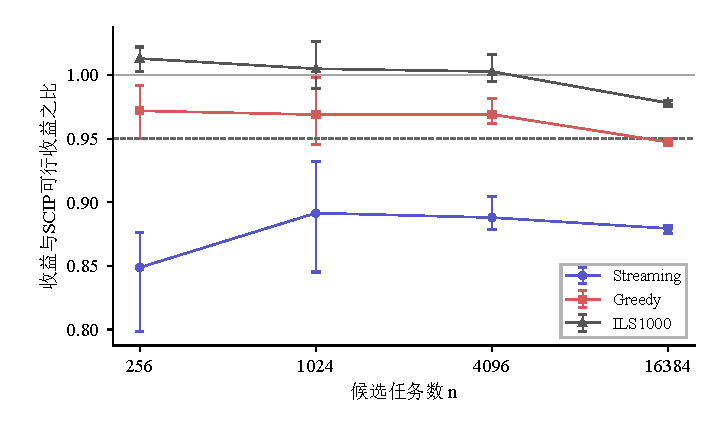
\includegraphics[width=120mm]{figures/controlled_n_quality.pdf}
 \caption{候选数各水平的质量比。点为三个结构种子的$h/L$均值，范围线为最小值至最大值，非置信区间；$L$为SCIP可行收益。虚线为$0.95$，SCIP未证明最优时比值可大于1。}
 \label{s0307:fig_n_quality}
\end{figure}

\begin{figure}[tbp]
 \centering
 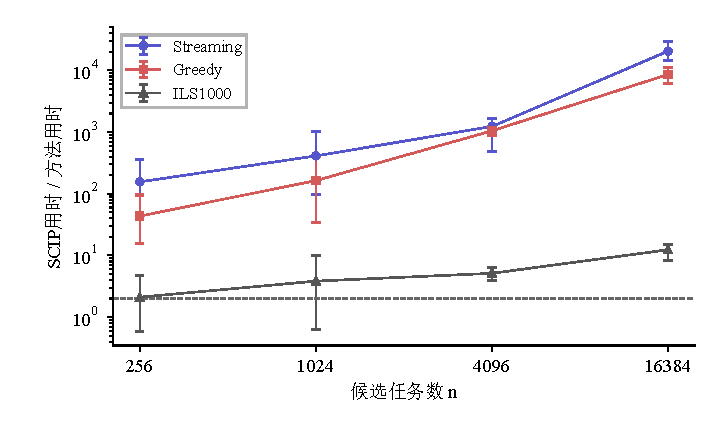
\includegraphics[width=120mm]{figures/controlled_n_time_ratio.pdf}
 \caption{候选数各水平的时间比。点为三个结构种子的$T_{\mathrm{SCIP}}/T_a$均值，范围线为最小值至最大值，非置信区间；比值大于1表示方法$a$在该条件下用时较短，虚线为2。}
 \label{s0307:fig_n_time}
\end{figure}

\paragraph{任务阶数。}
图\ref{s0307:fig_rank_quality}和图\ref{s0307:fig_rank_time}覆盖$r=4,8,16,32$。Streaming的平均质量比依次约为$0.8487$、$0.7992$、$0.7502$和$0.7054$，Greedy为$0.9718$、$0.8970$、$0.8657$和$0.8136$，ILS1000为$1.0128$、$0.9882$、$0.9694$和$0.9147$。在这组配对输入上，三种方法相对于SCIP可行值的平均质量比均随阶数水平提高而下降。

时间比却没有抵消质量损失：在$r=32$时，Streaming、Greedy和ILS1000的平均时间比分别约为11846、5984和313，但联合支持数分别为$0/3$、$0/3$和$1/3$。ILS1000在$r=8$时获得$3/3$支持，在$r=16$时降为$2/3$，在$r=32$时进一步降为$1/3$。可见，很大的时间比并不足以保证联合判据成立。这些数据揭示的是当前构造、收益与停止协议下的结果变化；它们没有单独测量内部搜索行为，不能据此认定某种未经检验的算法机制。

\begin{figure}[tbp]
 \centering
 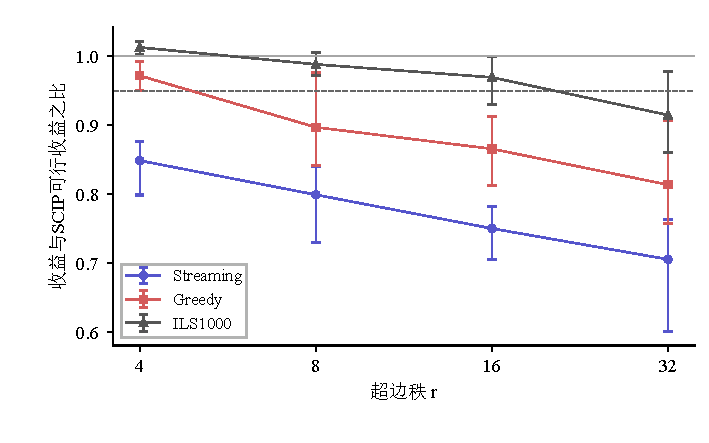
\includegraphics[width=120mm]{figures/controlled_rank_quality.pdf}
 \caption{任务阶数各水平的质量比。点为三个结构种子的$h/L$均值，范围线为最小值至最大值，非置信区间；$L$为SCIP可行收益。虚线为$0.95$，SCIP未证明最优时比值可大于1。}
 \label{s0307:fig_rank_quality}
\end{figure}

\begin{figure}[tbp]
 \centering
 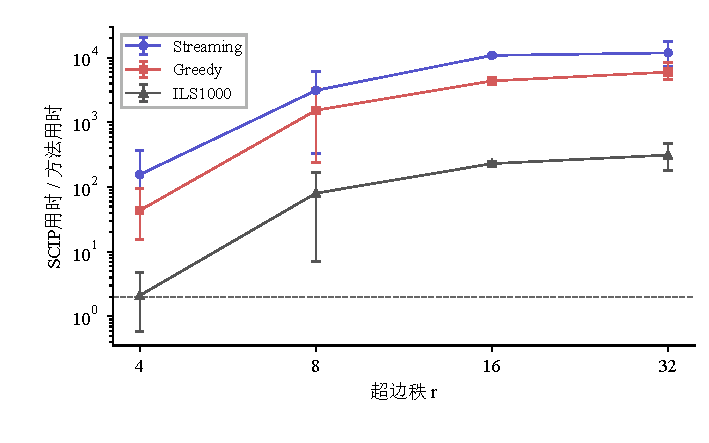
\includegraphics[width=120mm]{figures/controlled_rank_time_ratio.pdf}
 \caption{任务阶数各水平的时间比。点为三个结构种子的$T_{\mathrm{SCIP}}/T_a$均值，范围线为最小值至最大值，非置信区间；比值大于1表示方法$a$在该条件下用时较短，虚线为2。}
 \label{s0307:fig_rank_time}
\end{figure}

\paragraph{资源度。}
图\ref{s0307:fig_degree_quality}和图\ref{s0307:fig_degree_time}给出$\Delta=4,8,16,32$。Streaming平均质量比依次约为$0.8487$、$0.7620$、$0.8006$和$0.6867$，其中从8到16出现回升，不能概括为逐水平单调下降。Greedy平均质量比分别约为$0.9718$、$0.9516$、$0.9030$和$0.9200$，也存在非单调变化。虽然前节构造保证资源组粗化后的可行域嵌套，但相对于不同SCIP可行解计算的启发式质量比并无相应单调性保证。

ILS1000在$\Delta=8$和16时平均质量比分别为$0.9867$和$0.9865$，平均时间比分别为$6.8517$和$30.7168$，两个配置均获得$3/3$联合支持。到$\Delta=32$时，其平均质量比降为$0.9411$，平均时间比为$4.4089$，联合支持仅为$1/3$。从原值看，该水平的三个条件中ILS1000收益分别为510、502和478，对应SCIP收益536、527和520；时间比分布也跨越联合判据的界限。配置均值只能表达中心位置，不能替代逐种子的质量与时间配对。

\begin{figure}[tbp]
 \centering
 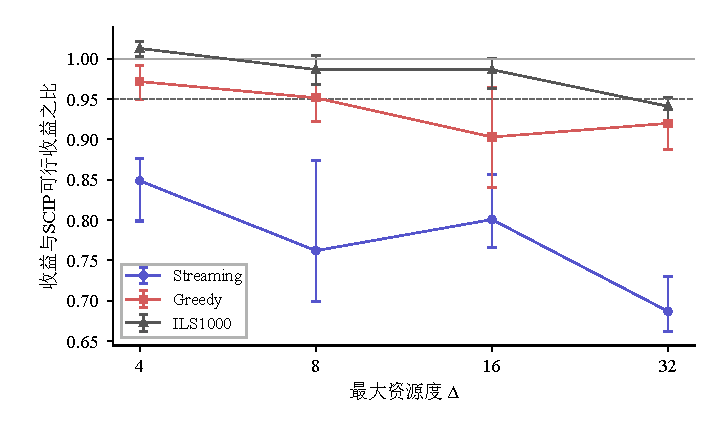
\includegraphics[width=120mm]{figures/controlled_degree_quality.pdf}
 \caption{资源度各水平的质量比。点为三个结构种子的$h/L$均值，范围线为最小值至最大值，非置信区间；$L$为SCIP可行收益。虚线为$0.95$，SCIP未证明最优时比值可大于1。}
 \label{s0307:fig_degree_quality}
\end{figure}

\begin{figure}[tbp]
 \centering
 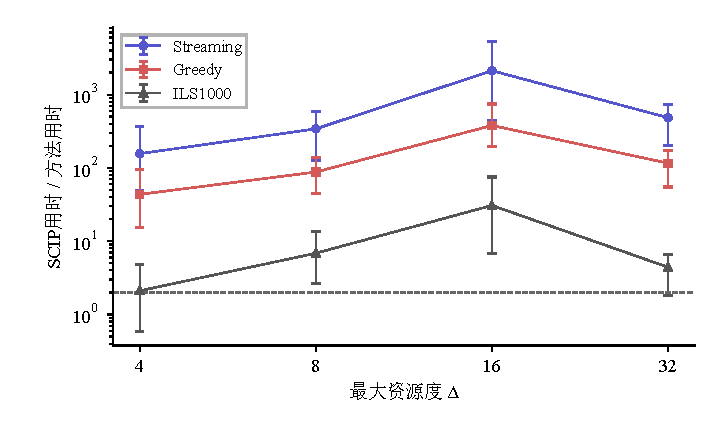
\includegraphics[width=120mm]{figures/controlled_degree_time_ratio.pdf}
 \caption{资源度各水平的时间比。点为三个结构种子的$T_{\mathrm{SCIP}}/T_a$均值，范围线为最小值至最大值，非置信区间；比值大于1表示方法$a$在该条件下用时较短，虚线为2。}
 \label{s0307:fig_degree_time}
\end{figure}

\paragraph{收益跨度。}
图\ref{s0307:fig_spread_quality}和图\ref{s0307:fig_spread_time}按$W=1,10,100,1000$展示全部水平，其中$W=100$为基准。Streaming平均质量比依次为$0.7692$、$0.8169$、$0.8487$和$0.9045$，Greedy为$0.7634$、$0.9217$、$0.9718$和$0.9785$。这两种方法在所列输入上的平均质量比随跨度增大而提高，但Streaming直到$W=1000$也仅有一个种子满足联合条件，Greedy在该水平也只有$2/3$支持。

ILS1000的平均质量比依次为$0.9764$、$1.0013$、$1.0128$和$1.0015$，对应平均时间比约为52559、$56.4644$、$2.1058$和$0.8888$。在$W=1$时，SCIP三个调用分别耗时$518.43\,\mathrm{s}$、$3163.6\,\mathrm{s}$和$3108\,\mathrm{s}$，ILS1000分别为$0.044125\,\mathrm{s}$、$0.075965\,\mathrm{s}$和$0.029804\,\mathrm{s}$，所以得到很大的时间比。到$W=1000$时，SCIP三个调用均约为$0.02\,\mathrm{s}$，ILS1000调用也处于这一量级，其时间比最大值只有$1.1823$，三个种子均未达到2。因此，ILS1000在$W=1000$虽保持或超过SCIP可行收益，联合支持仍为$0/3$。这一变化由所列收益与计时直接支持；仅凭曲线不足以进一步断定搜索树、归约作用或缓存行为的原因。

\begin{figure}[tbp]
 \centering
 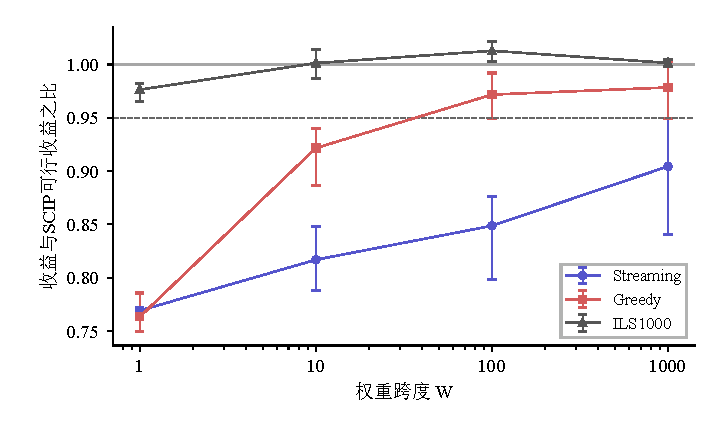
\includegraphics[width=120mm]{figures/controlled_spread_quality.pdf}
 \caption{收益跨度各水平的质量比。点为三个结构种子的$h/L$均值，范围线为最小值至最大值，非置信区间；$L$为SCIP可行收益。虚线为$0.95$，SCIP未证明最优时比值可大于1。}
 \label{s0307:fig_spread_quality}
\end{figure}

\begin{figure}[tbp]
 \centering
 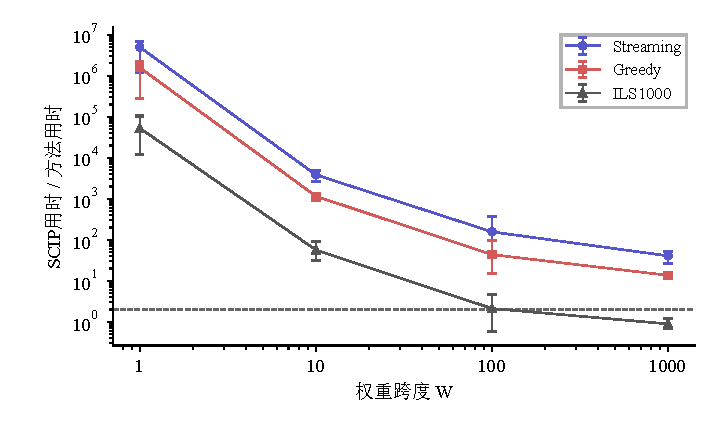
\includegraphics[width=120mm]{figures/controlled_spread_time_ratio.pdf}
 \caption{收益跨度各水平的时间比。点为三个结构种子的$T_{\mathrm{SCIP}}/T_a$均值，范围线为最小值至最大值，非置信区间；比值大于1表示方法$a$在该条件下用时较短，虚线为2。}
 \label{s0307:fig_spread_time}
\end{figure}

上述13组是既定开发条件下的完整描述。得到$3/3$支持的配置不能在观察结果后另行组成一个独立评价集；共享基准、结构种子及构造关系的配置也不能作为独立样本进行跨组显著性解释。本节不报告跨组$p$值。所有输入仍为单位容量，较大任务阶数不改变其可行域可由两两冲突表达的事实，因而这些曲线本身也不构成不可约高阶依赖或超图表示优势的证明。

\subsection{原作者完整流程的有效结果与失败分母}

原作者完整流程包含至多10轮归约、$S,\mathrm{pin}$贪心构造、ILS15和展开，不能与前述单独调用Greedy或ILS1000混为同一方法\cite{GrossmannJRS2026}。其中15是连续未改进计数的停止阈值，改进后计数重置，并非固定总迭代次数。七个既有公开输入各计划运行十个固定算法种子，共70次；实际65次有效、5次失败。表\ref{tab:author_results}同时保留计划分母、失败数以及有效输出的收益和时间统计。

{\small\setlength{\tabcolsep}{4pt}
\begin{longtable}{lrrrrrr}
\caption{公开完整流程的全部预定种子与有效子集结果}\label{tab:author_results}\\
\toprule
实例 & 有效/计划 & 失败 & 有效均值 & 有效最小 & 有效最大 & 有效均时/s\\
\midrule
\endfirsthead
\toprule
实例 & 有效/计划 & 失败 & 有效均值 & 有效最小 & 有效最大 & 有效均时/s\\
\midrule
\endhead
\midrule
\multicolumn{7}{r}{续下页}\\
\endfoot
\bottomrule
\endlastfoot
ibm01 & 10/10 & 0 & 257814 & 257521 & 258013 & 0.099067\\
ibm02 & 9/10 & 1 & 379719.3333 & 379495 & 379987 & 0.14808\\
us04 & 6/10 & 4 & 978 & 933 & 1065 & 12.339\\
bibd49 & 10/10 & 0 & 2289.9 & 2288 & 2307 & 0.022158\\
AProVE01 & 10/10 & 0 & 132908.6 & 132820 & 133005 & 0.086438\\
AProVE27 & 10/10 & 0 & 154209.6 & 154055 & 154455 & 0.071669\\
superblue19 & 10/10 & 0 & 11405360.9 & 11405242 & 11405475 & 7.9381\\
\end{longtable}
}
均值仅按有效子集计算；ibm02和us04分别有1和4个失败种子，其全十种子收益均值未定义，不能把失败计为零或删除后称完整统计。


为明确均值的适用对象，令$p$表示表中的一个公开输入，$\mathcal S_p$为其十个计划种子的集合，$\mathcal V_p\subseteq\mathcal S_p$为获得有效输出的种子集合。记$h^{\mathrm{full}}_{p,s}\geq0$为有效输出的无量纲收益，$T^{\mathrm{full}}_{p,s}>0$为对应调用时间，单位为$\mathrm{s}$。对$|\mathcal V_p|>0$的输入，表中有效均值定义为
\begin{align}
 \overline h^{\mathrm{valid}}_p
 &=\frac{1}{|\mathcal V_p|}
   \sum_{s\in\mathcal V_p}h^{\mathrm{full}}_{p,s},
 \label{s0307:author_quality_mean}\\
 \overline T^{\mathrm{valid}}_p
 &=\frac{1}{|\mathcal V_p|}
   \sum_{s\in\mathcal V_p}T^{\mathrm{full}}_{p,s}.
 \label{s0307:author_time_mean}
\end{align}
有效最小值和最大值也只在$\mathcal V_p$上取值。失败种子没有可用于上述收益平均的有效输出，不能赋零，也不能删除失败后将有效均值称为全十种子均值。

\texttt{ibm02}仅有$9/10$有效，所列379719.3333是九个有效结果的均值；\texttt{us04}仅有$6/10$有效，所列978是六个有效结果的均值。二者的全十种子收益均值均未定义。其余五个输入为$10/10$有效，才可将有效子集均值同时解释为全计划种子的均值。65次有效输出已经按原始权重和单位容量重新核验，这一事实不消除另外五次失败。

在\texttt{ibm01}上，完整流程十次收益介于257521和258013之间，均值257814，相对于SCIP最优收益265302仍少7488；有效平均调用时间为$0.099067\,\mathrm{s}$。因此，完整流程相对于Streaming收益219983有明显提高，但没有达到该输入的已知最优收益。\texttt{bibd49}的完整流程平均收益为2289.9，有效平均时间为$0.022158\,\mathrm{s}$，SCIP最优收益为2361；这同样是较短记录时间与收益差距并存的情形。

\texttt{us04}给出了不利结果：六个有效输出的收益从933到1065，最高值达到SCIP最优收益1065，但均值只有978；有效平均时间为$12.339\,\mathrm{s}$，长于SCIP历史记录的$2.5119\,\mathrm{s}$，且另外四个计划种子失败。不能只保留达到1065的输出来代表该流程。\texttt{superblue19}的十个有效输出则较集中，收益从11405242到11405475，均值11405360.9，有效平均时间为$7.9381\,\mathrm{s}$；SCIP保存的可行收益为11642395，按间隙结束。这一组记录支持对所得收益和调用成本作具体比较，但两种停止机制不同，不能扩展为统一预算下的全局优越性结论。

\subsection{三个条件上的九次停止阈值诊断}

最后考察三个既有条件上的Greedy、ILS1000和ILS5000诊断运行。三种输入分别为最大任务阶数12的1000候选合成条件、500顶点度为3的MIS转换条件，以及\texttt{ibm01}；对应编号为C06、C20和C26。各诊断调用使用算法种子0，九次输出均通过可行性核验。表\ref{s0307:tab_diagnostic}列出全部收益、选中任务数及调用时间。选中任务数是非负整数，表示二元变量中取值为1的项数，不能在非等权条件下代替收益。

\begin{table}[tbp]
 \centering
 \small
 \caption{三个既有条件的全部九次诊断运行}
 \label{s0307:tab_diagnostic}
 \begin{tabular}{llrrr}
 \toprule
 条件 & 方法 & 收益 & 选中任务数 & 时间/$\mathrm{s}$\\
 \midrule
 C06 & Greedy  & 694    & 8    & 0.0043294\\
 C06 & ILS1000 & 770    & 9    & 1.30735\\
 C06 & ILS5000 & 770    & 9    & 5.95733\\
 C20 & Greedy  & 182    & 182  & 0.0019908\\
 C20 & ILS1000 & 221    & 221  & 0.0593483\\
 C20 & ILS5000 & 222    & 222  & 0.193667\\
 C26 & Greedy  & 240686 & 4017 & 0.0301111\\
 C26 & ILS1000 & 263094 & 4085 & 33.9920\\
 C26 & ILS5000 & 264387 & 4063 & 107.008\\
 \bottomrule
 \end{tabular}
\end{table}

C06中，Greedy取得694，ILS1000提高到770，但ILS5000仍为770，调用时间却由约$1.31\,\mathrm{s}$增至$5.96\,\mathrm{s}$。因此，更大的停止阈值没有在该诊断中带来收益改进。两个ILS结果都高于初始SCIP限时收益740，这与其限时停止状态一致，不能据此宣称已知该条件最优值为770。

C20的目标为所选独立集大小，任务等权，所以收益与选中任务数相同。Greedy为182，低于初始Streaming的188；ILS1000提高到221，ILS5000进一步提高到222。与表\ref{tab:initial_results}中后续SCIP可行值221相比较，ILS5000多选了一个任务，但SCIP仍为间隙终止，222也没有因此获得最优性证明。

C26中，ILS1000从Greedy收益240686提高到263094，ILS5000进一步取得264387，但仍比SCIP最优收益265302少915。两次ILS调用分别耗时约$33.99\,\mathrm{s}$和$107.01\,\mathrm{s}$，均长于SCIP历史最优记录的$1.8463\,\mathrm{s}$。同时，ILS5000选中4063项任务，少于ILS1000的4085项，却取得更高收益；这直接说明正权加权任务选择应以权重总和评价，不能只比较接受任务数量。

ILS1000和ILS5000是分别启动的两次运行，即使使用相同算法种子，也不能未经轨迹核验就把前者视为后者的搜索前缀。阈值表示连续未改进计数，发现改进后重置，代码在计数大于阈值时停止\cite{GrossmannJRS2026}。因此，1000与5000不表示固定总迭代数，也不是相同墙钟预算。九次诊断展示了提高、保持和额外时间成本三类实际现象，支持逐输入讨论停止设置，不支持更大阈值必然改善收益或任一方法全局占优的结论。

\setcounter{section}{7}
\section{失败、反例和适用范围}
\label{sec:03_08}

第\ref{sec:03_07}节的结果同时包含收益差距、停止时尚未闭合的最优性间隙，以及未取得可验收输出的运行。这些现象回答不同的问题：收益差距说明一个可行选择还有多大改进空间，最优性间隙说明证明进行到什么程度，执行异常则说明某次调用没有完成预定的输出与验收过程。只有把这些含义分开，才能确定一项不利结果究竟限制了哪一个主张。

\subsection{可行性、最优性与运行终止的区别}

沿用前文的有限候选集合$E$、资源集合$V$及关联矩阵$A$。候选$e\in E$的选择量为$x_e\in\{0,1\}$，固定收益为$w_e>0$；$A_{ve}=1$表示任务$e$需要资源$v$的一份容量，否则为零。当前组合实验均取$b_v=1$。对一个已经取得的二元输出$\widehat x$，可行性要求每个资源的占用不超过一份，收益则按原输入重新求和。记其核验收益为$h=\sum_{e\in E}w_e\widehat x_e$，相同问题的最优收益为$z^\star$，二者均无量纲。

合法次优解要求已经知道$\widehat x$可行且$h<z^\star$。即使不知道精确的$z^\star$，只要另有一个核验可行解的收益严格高于$h$，也足以证明该输出次优。最优性未证则只表示现有证据不能判定$h=z^\star$：该输出可能已经最优，也可能仍可改进。因而，缺少最优性证书不能直接写成已经证明次优。

表\ref{s0308:status_meanings}将解的性质与运行状态分别列出。这些项目并非互斥分类。例如，一次资源保护退出可以留下待核验候选；一次正常结束的启发式调用可以返回合法次优解；一次限时结束的SCIP调用也可以留下可行解。

\begin{table}[tbp]
 \centering
 \small
 \caption{结果性质与运行状态的证据含义}
 \label{s0308:status_meanings}
 \begin{tabularx}{\linewidth}{@{}p{0.15\linewidth}XX@{}}
  \toprule
  项目 & 可以据此确认的内容 & 不能直接推出的内容\\
  \midrule
  合法次优解 & 原约束核验通过，且存在严格更好的可行收益或已知最优值 & 程序执行失败，或该解没有应用价值\\
  最优性未证 & 尚无足够证据确认当前收益达到全局最优 & 当前解必然次优，或原问题无解\\
  工程异常 & 某次调用在接口、原生执行或验收环节异常终止 & 原论文算法一般失效，或异常根因已经定位\\
  资源保护 & 外部资源管理条件触发了停止 & 算法正常完成，或已证明所需内存的严格峰值\\
  未完成或未验收 & 预定计算或输出验收尚未完成 & 未记录的输出可自动视为有效，或其目标值等于零\\
  \bottomrule
 \end{tabularx}
\end{table}

这一划分还排除了把求解失败解释为模型不可行的做法。对本章的基本选择模型，全零向量始终满足单位容量约束，式\eqref{s0203:zero_feasible}已经证明其可行域非空。某次程序没有返回可验收结果，不能推翻这一模型性质。全零选择的收益确实为零，但失败记录并不是程序返回并核验了全零选择的证据。

\subsection{收益反例限定的算法主张}

十二任务算例提供了一个可以完整核查的反例。枚举覆盖全部$4096$个二元选择，其中$62$个可行，唯一最优选择为$\{\mathrm{T02},\mathrm{T03},\mathrm{T04},\mathrm{T12}\}$，收益为$42$。Streaming返回$\{\mathrm{T01},\mathrm{T05}\}$，收益为$39$，且两种选择均将每项资源恰好占用一次。于是，该例同时满足
\begin{equation}
 \ell_v(x^{\mathrm S})=\ell_v(x^\star)=1,
 \quad\forall v\in V,
 \qquad
 z(x^{\mathrm S})=39<42=z(x^\star).
 \label{s0308:full_load_counterexample}
\end{equation}
这里$x^{\mathrm S}$与$x^\star$分别为第\ref{sec:02_07}节定义的Streaming选择和最优选择，$\ell_v$为资源$v$的占用份数，$z$为无量纲收益函数。相同的满负载对应不同收益，说明资源使用充分并不是收益最优的充分条件。Streaming输出已经不能直接追加任何非空资源任务，但撤销原选择后，仍能换入收益更高的组合。

该反例否定了Streaming在所有输入上都取得最优解，或都保持最优收益$95\%$的主张，因为$39/42\approx0.9286$。它没有否定第\ref{sec:03_02}节所述的、具有明确前提的近似保证\cite{ReinstadtlerFPU2025}，也没有否定这次输出的可行性。研究结论因此应落在具体的收益与成本取舍上，而不是把一次失优扩大为方法没有作用。

压力测试进一步限制了统一的高质量主张。59个条件的236次输出均通过容量和收益核验，但Streaming在S26的相对可行值比约为$0.6015$，Greedy在S28为$0.7500$，ILS1000在S16约为$0.8604$。这里的分母都是对应SCIP可行收益，未统一证明为最优值。这些反例已足以说明：三种方法都不能在所测全部条件上保证达到该参照收益的$95\%$。可行性全部通过与质量判据未全部通过并不矛盾。

时间与质量也须在同一输出上配对判断。例如，第\ref{sec:03_07}节的基准配置中，ILS1000平均质量比约为$1.0128$、平均时间比约为$2.1058$，但同时满足质量比不小于$0.95$和时间比不小于$2$的种子只有一个。两个均值分别过线，不能替代逐种子的联合判定。三个诊断条件还显示，增大停止阈值未必严格增加收益：C06的ILS1000与ILS5000均取得$770$，调用时间却分别约为$1.31\,\mathrm{s}$和$5.96\,\mathrm{s}$。这限制了更大阈值必然改善结果的说法；由于两次调用独立启动，也不能将其未经核验地解释为同一搜索轨迹的两个截点。

\subsection{原作者完整流程的五次失败及统计分母}

原作者完整流程在七个既有输入上各运行十个固定算法种子，共有70次预定调用，其中65次取得通过原始权重与容量核验的输出，5次没有可验收结果。该流程包括至多10轮归约、$S,\mathrm{pin}$贪心、ILS15和展开\cite{GrossmannJRS2026}。表\ref{s0308:failure_details}保留五次失败的输入、种子及可确认的终止现象。

\begin{table}[tbp]
 \centering
 \small
 \caption{原作者完整流程中未取得可验收结果的五次运行}
 \label{s0308:failure_details}
 \begin{tabularx}{\linewidth}{@{}llXX@{}}
  \toprule
  输入 & 种子 & 已观察现象 & 解释边界\\
  \midrule
  \texttt{ibm02} & 7 & 可行性与收益一致性的联合断言失败 & 日志不能区分哪一项失败，也不能确认二者是否同时失败\\
  \texttt{us04} & 1 & 原生调用抛出Windows异常\texttt{0xc00000ff} & 未定位到具体内存、栈或其他内部原因\\
  \texttt{us04} & 3 & RAM保护触发退出 & 无可验收输出；保护退出不表示正常搜索结束\\
  \texttt{us04} & 7 & 原生调用抛出Windows异常\texttt{0xc00000ff} & 与种子1具有相同异常码，不据此推定相同内部根因\\
  \texttt{us04} & 9 & RAM保护触发退出 & 无可验收输出；不能将收益记为零\\
  \bottomrule
 \end{tabularx}
\end{table}

\texttt{ibm02}的联合断言尤其需要保留逻辑含义。令$P$表示返回选择满足原容量约束，$Q$表示按原权重重算的收益与程序报告一致，二者均为真假命题。日志确认的是
\begin{equation}
 \neg(P\land Q)=\neg P\lor\neg Q.
 \label{s0308:assertion_logic}
\end{equation}
它说明至少一项检查未通过，却不蕴含单独的$\neg P$。因此，这条记录不能写成已经发现一个违反容量的解；收益不一致同样可能触发该联合断言。现有日志也不足以把失败定位到某一条归约或展开规则。

为描述这些失败对统计的影响，令$p$标识一个公开输入，$\mathcal S_p$为其十个计划种子的集合，$\mathcal V_p\subseteq\mathcal S_p$为取得有效输出的种子集合。集合元素是无量纲运行标识。定义观察失败比例
\begin{equation}
 f_p=\frac{|\mathcal S_p\setminus\mathcal V_p|}{|\mathcal S_p|}
 =1-\frac{|\mathcal V_p|}{10},
 \qquad f_p\in[0,1].
 \label{s0308:failure_fraction}
\end{equation}
$f_p$描述当前固定种子和执行环境下的记录比例，不是已经估计出的跨平台失败概率。有效子集均值仍按式\eqref{s0307:author_quality_mean}计算，并须与$f_p$并列。表\ref{s0308:conditional_statistics}列出两个存在失败的输入。

\begin{table}[tbp]
 \centering
 \small
 \caption{存在失败时的有效子集收益与计划覆盖}
 \label{s0308:conditional_statistics}
 \begin{tabular}{@{}lrrrrl@{}}
  \toprule
  输入 & 有效/计划 & 失败比例 & 有效收益均值 & 有效收益范围 & 全十种子均值\\
  \midrule
  \texttt{ibm02} & $9/10$ & $10\%$ & $379719.3333$ & $379495$--$379987$ & 未定义\\
  \texttt{us04} & $6/10$ & $40\%$ & $978$ & $933$--$1065$ & 未定义\\
  \bottomrule
 \end{tabular}
\end{table}

表中收益均为无量纲原权重之和。其余五个输入均为十次有效，才具备计算全十种子收益均值的完整输出。整体$5/70$约为$7.14\%$，但整体比例不能掩盖失败集中在两个输入上的事实。删除失败后得到的均值只描述有效输出子集；没有证据表明缺失与所得收益无关，故不能把它当作全部计划运行的收益均值。有效子集的平均调用时间也不包含失败尝试的全部投入，不能据此代表为完成整个计划付出的总成本。

这些失败是当前运行环境与移植执行中的观察。公开源码与本地适配范围的对应材料在附册中保留，优化内核未被重写；但源码来源本身并不能证明适配、执行及验收的每一环节都正确。五次失败限定了本次完整流程的完成率及可报告统计，不足以断言原论文算法错误，也不足以断言它在其他环境或输入上一般失效。

\subsection{已经核验的浮点边界与尚未定位的原因}

第\ref{sec:03_03}节将理想实数优先级与实际机器表达式分开说明。对\texttt{us04}的独立表达式核验已经确认：在163项任务中，118项任务的资源度连乘在所检查的IEEE~754双精度表达式中溢出为正无穷，相应机器优先级成为零。这是已取得证据的数值表达式边界，不能笼统写成浮点异常是否存在尚不清楚。

其组合含义是，式\eqref{s0303:unit_priority}中严格为正、可能彼此不同的理想优先级，在该机器表达式下有一批被合并为零分。此时，数学分数所规定的严格大小关系未必还能由机器分数区分，具体访问顺序需要结合并列处理规则解释。该事实不意味着这些任务的原始收益为零，也不意味着它们违反资源容量。

这次核验检查的是保留适配器中的双精度算术表达式，没有重新执行原生贪心过程，也没有修改公开优化内核。因此，已核验的零分合并不能直接解释某次完整运行的收益差、异常退出或RAM保护。完整流程使用的$S,\mathrm{pin}$静态分数见式\eqref{s0304:static_pin_score}，与第\ref{sec:03_03}节的度乘积优先级不同，更不能仅因输入同为\texttt{us04}就把两类现象建立为因果关系。

原生内核其他浮点运算的行为、机器整数中间量是否溢出，以及哈希容器遍历是否造成跨运行差异，仍须各自的执行证据才能判定。尤其是ILS接受规则中的整数乘积，其数学解释以中间运算没有溢出为条件；这一条件尚不能改写为本批运行已经发生整数溢出。同样，固定随机种子说明随机输入受到控制，但仅凭种子值不能证明所有平台上的容器遍历和搜索轨迹一致。

\subsection{停止协议、相关样本与资源测量的边界}

SCIP的$5\%$间隙停止与启发式停止承担不同任务。前者在有效上下界和正可行收益的条件下限制尚未排除的最优收益范围；Streaming结束表示完成既定扫描与逆序构造；ILS停止表示连续未刷新最好收益的计数超过阈值。ILS15、ILS1000和ILS5000中的数值都是这一计数阈值，改进后重置，不是固定总迭代次数，也不是墙钟时间预算。

因此，前节的时间比可以说明相应调用按各自规则结束时的耗时关系，却不能直接构成等预算速度排名。初始记录、压力测试和完整流程还存在热启动、计时边界及CPU并发差异。续跑继承的可行解具有先前获取成本；历史首次正收益记录也不能被解释为重新实施了统一时限实验。求解器运行中的目标和界只是报告快照，在缺少对应见证核验时不能作为已完成决策。

样本数量也须对应实际生成过程。92项实验条件中包含共享拓扑、改变权重以及具有嵌套关系的派生条件；七个完整流程输入已经包含其中。算法种子重复观察同一输入上的搜索变化，结构种子则参与输入生成，两者并非同一种重复。十二任务算例的21次重复测时没有增加独立实例数。由这些相关记录计算的均值、范围和联合支持数具有描述意义，不能把全部运行视为相互独立的样本，进而补出没有实施的显著性结论。

内存记录还有采样边界。设一次进程观察区间为$[0,T]$，其中$T>0$以$\mathrm{s}$计；$M(t)\geq0$表示时刻$t$的驻留集大小，即RSS，统一以字节计。若仅在$k$个时刻$t_1,\ldots,t_k\in[0,T]$采样，$k$为正整数，则在采样值准确且统计口径一致的条件下，
\begin{equation}
 M_{\mathrm{sample}}=\max_{1\leq i\leq k}M(t_i)
 \leq
 M_{\mathrm{sup}}=\sup_{t\in[0,T]}M(t).
 \label{s0308:memory_sampling}
\end{equation}
$M_{\mathrm{sample}}$是采样最大RSS，$M_{\mathrm{sup}}$是整个观察区间的RSS上确界，二者单位相同。采样间隙内可能存在未捕获的增长，因此不能将采样最大值标为严格峰值。RAM保护记录说明保护条件被触发，并不单独给出算法完成所需的最小内存；RSS与其他内存口径也不能混用。

\subsection{从组合选择到巡检执行的适用范围}

本章实验直接适用于候选任务及关联已固定、收益为正且可加、每个关联需求占用一份资源、全部容量为一的选择问题。对任意二元向量$x\in\{0,1\}^{|E|}$，有
\begin{equation}
 \left[\sum_{e\in E}A_{ve}x_e\leq1,
       \ \forall v\in V\right]
 \quad\Longleftrightarrow\quad
 \left[x_e+x_f\leq1,
       \ \forall e\ne f:\ R_e\cap R_f\ne\varnothing\right].
 \label{s0308:unit_capacity_boundary}
\end{equation}
这里$e,f\in E$为不同任务，$R_e,R_f$为各自需要的资源子集。左侧逐资源限制占用，右侧逐冲突任务对限制共选；等价性依赖二元域及单位容量。较大的超边秩只表示单项任务关联更多资源，并不破坏这一等价性。因此，当前实验没有仅凭高秩证明不可约高阶耦合，也没有通过表示之间的受控比较证明超图形式必然更快。整数可行域等价还不意味着连续松弛、存储成本和实际求解时间相同，相关区别见第\ref{sec:02_04}节。

这些边界同样限制向无人集群巡检的外推。纯组合选择没有给出连续轨迹、观测姿态、电池能量变化、车辆与无人机会合时序，以及设备服务后的再次使用过程。共享资源检查通过，只说明当前静态占用定义下没有冲突。要成为可执行巡检方案，还必须为同一选择提供共同满足物理与时序条件的执行见证；逐个任务可行并不保证任务之间能够同步执行。第\ref{sec:01_03}节的投影关系也以资源约束确实是执行过程的必要条件为前提，不能自动套用于任意静态设备占用定义。

本章记录的秒数是主机上的计算耗时，不是无人机飞行历时或现场测量。公开MIS输入的复用也不构成HypOp神经求解器的性能实验，因为该求解器没有运行。由本章收益与时间数字，既不能证明工程联合模型更优，也不能推出某个区域可以实现完整覆盖。

区域模型已有有限转录的构建与运行记录；没有取得新结果不能改写为没有实现。现有区域记录中，LP求解错误属于较早的绑定运行；截至2026年11月10日03:56 UTC的后续观察，最新运行因资源保护退出，留下的四塔候选仍需重新验收，尚无新验收的完整区域覆盖方案。候选目标数值相同不能代替执行见证一致，也不能继承其他版本的验收结论。这一状态说明当前证据尚未给出完整覆盖方案，并不证明原联合问题无解；其目标允许部分完成，亦不能悄然改写为全部杆塔必选。

由此进入第4章时，需要补充的是选择之外的物理对象与状态关系：先定义地理位置、观测要求和设备，再逐项建立运动、成像、安全与能量条件。只有这些条件与后续分配、航次和同步约束共同成立，组合层的选择才可能获得巡检层的执行含义。

\setcounter{section}{8}
\section{异构任务分配与联合优化方法}
\label{sec:03_09}

\subsection{共同原问题与集中求解}

异构任务分配需要同时确定执行主体、共享资源占用时序和能够实现任务的运动。比较求解方法，首先应保持这些决策对应的目标与可行域一致。记离散决策为 $x\in\mathcal X$，包括任务选择、主体分配和先后关系，$\mathcal X$ 为给定有限转录下的有限取值集合；连续决策为 $y\in\mathcal Y$，包括时刻、位置和能量，其分量分别采用 $\mathrm{s}$、$\mathrm{m}$、$\mathrm{Wh}$ 等对应单位。能力、平台、运动与能量约束共同定义
\begin{equation}
\label{s0309:shared_domain}
\mathcal F=\{(x,y)\in\mathcal X\times\mathcal Y:
 g_a(x,y)\leq0\ (a\in\mathcal A),\quad
 h_b(x,y)=0\ (b\in\mathcal H)\}.
\end{equation}
其中 $\mathcal A$、$\mathcal H$ 分别为不等式和等式索引集，各残差保留对应物理量的单位。该式是第\ref{sec:05_08}节完整约束的统一记法，不替代具体物理定义。

本书依次最小化未完成塔数、车队返回历时和机载耗能。词典序优化的数学定义要求：只有此前阶段的最优值已经取得并被证明，才能将这些最优值固定为后续阶段的约束。若仅取得可行上界，以该值继续优化只是条件优化，不能称为完整词典序全局最优。以下以 $f(x,y)$ 表示一个标量阶段的目标，单位沿用该阶段目标，前序最优值限制并入 $\mathcal F$。定义
\begin{align}
\label{s0309:value_function}
V(x)&=\inf_{y\in\mathcal Y}\{f(x,y):(x,y)\in\mathcal F\},\\
\label{s0309:decomposition}
\inf_{(x,y)\in\mathcal F}f(x,y)&=\min_{x\in\mathcal X}V(x).
\end{align}
这里假定 $\mathcal X$ 非空，空条件可行集的值约定为 $+\infty$。右端是有限集合上扩展实数值的最小化；要恢复实际最优方案，还须相应连续子问题取得有限下确界。写出 $\inf$ 并不证明问题有界，也不意味着数值计算已取得有效界。核验通过的可行解提供最小化问题的上界，有效松弛可提供下界。

集中方法输入完整参数、初态和约束，输出联合决策及求解状态。有限模型的目标与约束均线性时形成MILP；保留非线性运动、功率或几何关系时形成MINLP。集中组织便于统一检查共享资源，但承担信息汇集、模型存储和联合搜索成本，非凸模型的局部解也不自动具有全局最优性。式\eqref{s0309:decomposition}表明，计算分解可以保留统一目标和全部约束；若上游不可逆地固定 $x=\bar x$，下游则只求 $V(\bar x)$，一般会缩小原问题的搜索范围。

\subsection{拍卖分配与能力分布的接口}

CBBA将市场式任务选择与局部一致性过程结合\cite{CBBA2009}。用于上述原问题时，其输入包括任务、主体资格、评分和通信关系，输出任务归属候选。若评分只包含单机飞行代价，就未计入其他飞机占用平台引起的等待；共享时序检查必须反馈到评分或分配修正中，才能表达这种耦合。适配成本因此包括通信、重复评估和冲突协调。其保证依赖评分与通信连通性等条件，不能直接迁移为完整巡检模型的最优性保证。

STRATA接收任务能力需求、种群组成、随机能力模型和任务间转移关系，优化转移率，使主体分布达到所需能力配置\cite{STRATA2020}。此处引用2020年2月6日版本，初稿发表于2019年。令 $\mathcal C$ 为主体类别集，$\mathcal D$ 为能力类别集，$N_{ic}\geq0$ 为任务 $i\in\mathcal I$ 上类别 $c\in\mathcal C$ 的主体数量或连续分布近似，$Q_{cd}$ 为对应类别的随机能力量。对可累加能力集 $\mathcal D_{\mathrm{add}}\subseteq\mathcal D$，有
\begin{equation}
\label{s0309:trait_aggregation}
Y_{id}=\sum_{c\in\mathcal C}N_{ic}Q_{cd},
\qquad i\in\mathcal I,\ d\in\mathcal D_{\mathrm{add}}.
\end{equation}
$N_{ic}$ 为无量纲计数，$Y_{id}$ 与 $Q_{cd}$ 采用该能力的单位，不同能力列不能直接相加。该框架考虑类别间和个体间差异，并区分可累加与不可累加属性。对于速度、特殊技能等不可累加属性，采用阈值资格表示后统计达标主体数量，不能将多架飞机的速度相加。

能力分布回答的是任务获得了多少、何种能力。落到巡检执行时，还需将连续分布落实为整数主体及具体飞机身份，并接入物理电池、航次和平台时序。转移率及其分布动力学不直接给出这些资源的可执行日程，也不替代旋翼运动与能量约束。

\subsection{任务运动交替与不确定性反馈}

TAMP以动作前提、状态变化和连续几何约束为输入，联合搜索动作骨架与连续参数，输出满足动作约束的计划\cite{TAMP2021}。该文发表于2021年，作者预印本发表于2020年。巡检中的起飞、观测和会合可构成骨架，位置、时刻与轨迹用于检验其可实现性；适配需要建立动作接口、连续检查及反馈机制。

固定骨架后的NLP失败可能源于初始化、数值困难或搜索不足。只有证明整个条件可行集为空，才能据此排除骨架。例如，$x\in\{0,1\}^{d_x}$ 为长度 $d_x$ 的二进制编码，若 $\bar x$ 已被证明不存在任何可行连续补全，才可加入
\begin{equation}
\label{s0309:nogood}
\sum_{j:\bar x_j=1}(1-x_j)+
\sum_{j:\bar x_j=0}x_j\geq1,
\end{equation}
其中求和索引均取自 $\{1,\ldots,d_x\}$，各项无量纲。局部NLP失败不能生成这种全局有效的排除约束。任务优先、运动优先与交替搜索是任务和运动的组织方式，通信架构与规划适应性则是另外的分类维度\cite{MATAMP2026}；该综述于2026年5月23日在线发表，不是一个新增求解器。

不确定性处理仍应保留同一组物理约束，并限制决策使用的信息。设第 $k$ 次更新的已知初态与记录为 $H_k$，有限情形集合为 $\Xi_k$，情形 $\xi$ 下的完整决策为 $z^\xi=(x^\xi,y^\xi)$。令 $r$ 表示参与决策的主体，$\ell$ 表示其决策时刻，$H_{r\ell}^\xi$ 为该主体截至该时刻实际收到的信息历史。策略 $\pi$ 的动作必须对这些信息生成的 $\sigma$ 代数可测，不能使用其他主体尚未传达的信息。用 $\Pi_k^{\mathrm{info}}$ 表示满足此条件的策略集；其非预知性要求为
\begin{equation}
\label{s0309:nonanticipativity}
H_{r\ell}^{\xi}=H_{r\ell}^{\xi'}
\ \Longrightarrow\ 
\pi_{r\ell}(H_{r\ell}^{\xi})=
\pi_{r\ell}(H_{r\ell}^{\xi'}),
\qquad \forall r,\ell,\xi,\xi'.
\end{equation}
动作的单位随控制量或任务决策而定。给定无量纲概率 $p_\xi\geq0$ 且 $\sum_{\xi\in\Xi_k}p_\xi=1$，随机情景问题写为
\begin{equation}
\label{s0309:scenario}
\begin{aligned}
\min_{\pi}\quad &\sum_{\xi\in\Xi_k}p_\xi f(z^\xi;\xi)\\
\text{约束}\quad &z^\xi\in\mathcal F(H_k;\xi),\qquad \forall\xi\in\Xi_k,\\
&\pi\in\Pi_k^{\mathrm{info}}.
\end{aligned}
\end{equation}
在同一情形集上，鲁棒问题写为
\begin{equation}
\label{s0309:robust}
\begin{aligned}
\min_{\pi}\quad &\sup_{\xi\in\Xi_k}f(z^\xi;\xi)\\
\text{约束}\quad &z^\xi\in\mathcal F(H_k;\xi),\qquad \forall\xi\in\Xi_k,\\
&\pi\in\Pi_k^{\mathrm{info}}.
\end{aligned}
\end{equation}
两式中的 $z^\xi$ 均由策略和情形共同产生，目标沿用当前标量阶段的单位。这是本书的一般建模表达。情景方法需要概率依据，鲁棒方法需要有物理依据的不确定集合；前者不保证未纳入情形的表现，后者可能增加保守性。滚动优化只执行当前决策段，再依据新信息更新，其成本包括多情形计算和状态接续。当前已有观测状态接续组件，但完整区域的规划、执行与重规划尚未形成闭环。

\subsection{共享平台的完整教学算例}

本书构造算例B说明分配与时序的相互作用。两个任务为 $J_1,J_2$，两架飞机为 $U_1,U_2$；$J_1$ 可由任一飞机执行，$J_2$ 只能由 $U_2$ 执行。两任务在时刻零释放，共享起飞平台容量为1，每次平台服务持续 $3\,\mathrm{min}$。全部飞行时长见表\ref{s0309:parameters}。
\begin{table}[htbp]
\centering
\caption{教学算例B的任务飞行时长}
\label{s0309:parameters}
\begin{tabular}{ccc}
\toprule
飞机 & $J_1$（$\mathrm{min}$） & $J_2$（$\mathrm{min}$）\\
\midrule
$U_1$ & 10 & 不具资格\\
$U_2$ & 12 & 8\\
\bottomrule
\end{tabular}
\end{table}

本例省略返航、电池和路线，以最晚巡检完成时间为目标；同机下一次起飞服务必须等待前一任务完成。令 $a_j$ 为任务 $J_j$ 的飞机编号，$s_j,C_j$ 分别为平台服务开始和巡检完成时刻，$C_{\max}$ 为最晚完成时刻，三者以 $\mathrm{min}$ 计；$d_{a_j,j}$ 为表中合法组合的飞行时长。完整模型为
\begin{align}
\label{s0309:example_model}
\min\;&C_{\max},\\
a_1&\in\{1,2\},\qquad a_2=2,\\
s_j,C_j&\geq0\quad(j\in\{1,2\}),\qquad C_{\max}\geq0,\\
C_j&=s_j+3+d_{a_j,j},\quad
C_{\max}\geq C_j,\qquad j\in\{1,2\},\\
(s_1+3\leq s_2)&\ \lor\ (s_2+3\leq s_1),\\
a_1=a_2&\ \Longrightarrow\
\bigl[(C_1\leq s_2)\lor(C_2\leq s_1)\bigr].
\end{align}
平台析取约束禁止服务重叠，最后一行禁止同机任务重叠，二者分别限制平台和飞机。

采用Python全枚举与算术重算，遍历两种分配及两种平台顺序。固定分配和顺序后，推迟服务不会降低最晚完成时间，故取满足资源限制的最早开始时刻即可得到该组合的最优日程。
\begin{table}[htbp]
\centering
\caption{全部分配与平台顺序的最早日程}
\label{s0309:enumeration}
\begin{tabular}{ccccc}
\toprule
$(a_1,a_2)$ & 平台顺序 & $(s_1,s_2)$ & $(C_1,C_2)$ & $C_{\max}$\\
 & & $\mathrm{min}$ & $\mathrm{min}$ & $\mathrm{min}$\\
\midrule
$(1,2)$ & $J_1,J_2$ & $(0,3)$ & $(13,14)$ & 14\\
$(1,2)$ & $J_2,J_1$ & $(3,0)$ & $(16,11)$ & 16\\
$(2,2)$ & $J_1,J_2$ & $(0,15)$ & $(15,26)$ & 26\\
$(2,2)$ & $J_2,J_1$ & $(11,0)$ & $(26,11)$ & 26\\
\bottomrule
\end{tabular}
\end{table}

同一分配因平台顺序不同得到14和16分钟，单机执行的两种顺序均为26分钟。因此该模型的枚举最优值为14分钟，而任务归属本身尚不足以确定联合目标。上述结果属于本书教学模型的完整有限枚举，不是SCIP、CBBA或其他公开算法的复现与性能比较；其最优性仅针对本例列明的约束，不构成区域巡检方案的验收结论。

\setcounter{section}{9}
\section{具身协作与学习规划方法}
\label{sec:03_10}

\subsection{观测、记忆与动作的接口}

第\ref{sec:03_09}节的联合优化以明确参数和可行域为基础。具身协作还需要回答：主体实际看到了什么，如何保留执行历史，以及规划动作能否由当前设备完成。为比较不同方法，下面建立本书的通用接口表达；它不是所引论文共有的算法或定理。

令 $\mathcal R$ 为参与协作的机器人集合，$r\in\mathcal R$ 为主体，$k\in\mathbb N_0$ 为决策事件编号。主体在该事件收到的观测为 $o_{rk}\in\mathcal O_r$，记忆为 $M_{rk}\in\mathcal M_r$，能力记录为 $C_{rk}\in\mathcal C_r$。三个集合分别表示观测、记忆和能力记录的允许取值。观测包含传感信息及已到达消息；记忆保存任务进度、已执行动作和失败原因；能力记录描述传感器、运动机构及当前健康状态。它们都是结构化对象，不具有统一单位，其中位置、时间和能量字段分别沿用 $\mathrm{m}$、$\mathrm{s}$ 和 $\mathrm{Wh}$，资格标记为无量纲布尔量。

令 $H_{rk}$ 为该主体截至事件 $k$ 实际收到的信息历史，$\mathcal A_r$ 为其技能及控制参数组成的动作空间，$\mathcal A_r^{\mathrm{info}}(H_{rk},C_{rk})\subseteq\mathcal A_r$ 为按已知信息筛选的候选动作集合。给定任务描述 $T$，策略产生动作提议
\begin{equation}
\label{s0310:policy_interface}
a_{rk}^{\mathrm{prop}}\sim
\pi_r(\cdot\mid o_{rk},M_{rk},C_{rk},T),
\qquad
\operatorname{supp}\pi_r\subseteq
\mathcal A_r^{\mathrm{info}}(H_{rk},C_{rk}),
\quad r\in\mathcal R.
\end{equation}
这里 $\pi_r$ 为动作概率分布，确定性选择是其特例；离散技能名称无量纲，连续参数采用对应控制量的单位。记忆和能力更新只能使用已收到的信息，因此相同信息历史应满足式\eqref{s0309:nonanticipativity}的非预知性要求。

候选集合表达的是信息条件下的判断。传感延迟可能使其中仍含物理上已不可执行的动作，而且各主体分别合法也不保证共享平台或联合轨迹合法。因此，动作提议还须经过执行前检查，执行后再形成反馈。令 $f_{rk}\in\mathcal F_r^{\mathrm{fb}}$ 为下一决策前收到的反馈，$\mathcal F_r^{\mathrm{fb}}$ 为反馈记录空间，则记忆更新写为
\begin{equation}
\label{s0310:memory_update}
M_{r,k+1}=\Psi_r(M_{rk},a_{rk}^{\mathrm{prop}},f_{rk}),
\qquad r\in\mathcal R,
\end{equation}
其中 $\Psi_r$ 为记忆更新规则。反馈应区分提议被拒绝、动作已执行、部分完成和完成验收，并附带相关观测及接收时刻。讨论中提出一个动作，不能直接把其预期后果写成已发生状态。

\subsection{能力描述、反馈规划与协作评价}

EMOS研究不同具身能力如何进入任务分解与分配\cite{EMOS2025}。其Robot Resume由URDF骨架的语言概括和正运动学计算共同生成，包含移动、感知和操作能力的文字及数值描述。系统接收任务、场景上下文和机器人能力档案，通过集中讨论形成子任务分配，再由各主体调用专属技能并行执行，以动作响应更新历史。能力档案因而连接任务要求与具体机构，而不是仅给机器人附加角色名称。

这一接口依赖论文明确采用的理想语义与几何重建：初始几何观测来自完美多机器人SLAM假设。其基准关闭了集成的PyBullet接触物理，并将接触到的抓取物吸附到夹爪。由此得到的任务执行结果不能证明巡检飞行、电池或接触动力学正确；机器人几何模型也不能替代本书的功率与续航模型。

COHERENT研究长时域异构任务中的提议、执行、反馈与调整，即PEFA循环\cite{COHERENT2025}。集中分配器输入任务指令、能力、各机器人局部观测及历史，输出带主体身份的子任务；执行器根据当前状态生成的动作列表选择动作，并检查其可执行性。反馈再区分任务分解错误、主体资格错误和执行受限，推动下一次提议。其局部观测不包含其他房间或关闭容器内的全部对象，因此记录历史并不等于获得完整环境状态。

该基准包含100项任务，主比较选取其中40项，覆盖5个场景，每场景8项，合计10项单类型、15项双类型和15项三类型任务。表\ref{s0310:coherent_results}仅转述论文表II的整体均值。
\begin{table}[htbp]
\centering
\caption{COHERENT论文自报的40任务比较结果}
\label{s0310:coherent_results}
\begin{tabular}{lcc}
\toprule
方法 & 成功率SR & 平均步数AS\\
\midrule
COHERENT & 0.975 & 12.4\\
移除历史 & 0.750 & 16.5\\
\bottomrule
\end{tabular}
\end{table}

令 $\mathcal Q$ 为这40项任务的集合，$G_q$ 为作者人工设计的参考完成步数，$b_q\in\{0,1\}$ 表示任务是否在 $2G_q$ 步内完成全部要求，$L_q$ 为成功时的执行步数。论文的统计规则可写为
\begin{align}
\label{s0310:coherent_metrics}
\mathrm{SR}&=\frac{1}{|\mathcal Q|}\sum_{q\in\mathcal Q}b_q,\\
\mathrm{AS}&=\frac{1}{|\mathcal Q|}\sum_{q\in\mathcal Q}\widetilde L_q,
&\widetilde L_q&=
\begin{cases}
L_q,&b_q=1,\\
2G_q+1,&b_q=0.
\end{cases}
\end{align}
成功率无量纲，步数为离散计数。失败记录保留在平均值中；完整方法的成功率仍未达到全部成功。该对照支持历史在此设置中的作用，但基准步数不是运行时间，也不包含训练、推理及通信的全部成本。这些结果不是本项目复现，不能据此作跨论文排名。

PARTNR的研究对象是家庭环境中的人机协作评价\cite{PARTNR2025}。它以自然语言任务、初始场景和主体能力约束构成问题，区分空间关系、时间顺序及只能由特定主体完成的操作。被评估规划器根据世界图和动作历史选择技能；评价函数则输入完整执行状态序列，输出完成比例、成功与否及失败解释。检查整段序列可以识别顺序错误，避免只看终态而漏掉过程要求。论文分别考察规划、感知和技能执行，报告了任务跟踪、伙伴协调及技能失败恢复方面的困难。这说明能力描述、执行反馈和独立评价承担不同功能。EMOS、COHERENT与PARTNR均不能据此被称为通用超图求解器。

\subsection{学习策略在执行链中的位置}

强化学习通过交互回报改进动作策略。HARL允许各主体使用不同参数及不同动作空间，以多主体优势分解组织贡献评估，并顺序更新策略，使后更新者考虑先更新者的变化\cite{HARL2024}。其训练输入包括交互状态、动作及共同奖励，输出异构策略；在线阶段由策略产生动作。顺序更新指训练过程，不要求机器人依次串行执行。理论推导采用完全可观测等条件，实践中的局部观测或记忆网络不能直接继承其全部保证。用于巡检还须建立训练环境、奖励和约束接口，奖励最大化也不自动等价于本书词典序目标。

模仿学习从示范中的观测与动作对应关系学习技能。NoMaD以当前及历史RGB观测、可选目标图像为输入，通过目标遮蔽统一探索与目标导航，再由扩散策略输出短时域未来动作序列，并配合拓扑记忆进行长程导航\cite{NoMaD2024}。其作用层是地面机器人的导航技能，训练依赖机器人轨迹数据。迁移时需要核对视觉条件、动作尺度和底层控制接口；已有地面导航证据不能推出多无人机调度或飞行安全保证。

OpenVLA将图像和语言指令映射为机器人操作动作，以示范数据训练动作标记预测，再将预测解码为末端位姿变化和夹爪控制\cite{OpenVLA2024}。它处于视觉语言条件下的操作策略层，适配新设备涉及动作编码、相机配置与目标域数据，并可采用微调。多种机器人上的操作能力不等于输出车队任务计划。NoMaD和OpenVLA均未在本巡检系统接入。

世界模型可在本书的接口中承担候选动作后果预测：根据当前状态估计与动作，预测后续观测或状态，供规划器比较方案。这是方法作用位置的说明，不是本项目已有实现结果。预测状态不能替代执行证据，模型误差仍须通过新观测修正。

这些方法的成本应分开计量。离线部分包括数据采集、训练、微调和验证；在线部分包括感知、记忆维护、策略推理、候选预测、通信及动作检查。扩散动作生成涉及迭代推理，语言规划涉及反复调用，预训练模型也有加载和设备适配成本。仅比较一次策略前向计算，不能代表闭环任务成本。

\subsection{故障消息到达后的合法反馈}

本书构造的教学算例C只考察热成像资格随消息接收的变化。飞机为 $U_1,U_2$，任务 $J_2$ 必须使用热成像，初始只有 $U_2$ 具备该能力。热成像故障发生于 $4\,\mathrm{min}$，规划端于 $6\,\mathrm{min}$ 收到消息；其间没有其他揭示故障的信息。令 $t\geq0$ 为以 $\mathrm{min}$ 计的时间，$\mathcal K^{\mathrm{th}}(t)$ 为实际热成像能力主体集，$\widehat{\mathcal K}^{\mathrm{th}}(t)$ 为规划端记录的能力主体集，则
\begin{align}
\label{s0310:failure_capability}
\mathcal K^{\mathrm{th}}(t)&=
\begin{cases}
\{U_2\},&0\leq t<4,\\
\varnothing,&t\geq4,
\end{cases}\\
\widehat{\mathcal K}^{\mathrm{th}}(t)&=
\begin{cases}
\{U_2\},&0\leq t<6,\\
\varnothing,&t\geq6.
\end{cases}
\end{align}
设 $a^{\mathrm{th}}(r,J_2)$ 表示将热成像任务交给主体 $r$ 的离散动作。仅按热成像资格筛选的候选动作集为
\begin{equation}
\label{s0310:failure_actions}
\widehat{\mathcal A}^{\mathrm{th}}(t)
=\{a^{\mathrm{th}}(r,J_2):r\in\widehat{\mathcal K}^{\mathrm{th}}(t)\}
=\begin{cases}
\{a^{\mathrm{th}}(U_2,J_2)\},&0\leq t<6,\\
\varnothing,&t\geq6.
\end{cases}
\end{equation}
该集合不表示平台、航迹及能量约束已经通过。在区间 $[4,6)$，信息候选仍保留 $U_2$，实际热成像动作却已不可执行；消息延迟不能被解释为动作仍然安全有效，也不能允许规划器提前使用尚未收到的故障信息。

已有Python算术重算给出的结果是：消息接收后，热成像资格集合为空，$J_2$ 仍未完成。$U_1$ 的可见光能力不能替代热成像，因此合法反馈应撤销失效资格、保留未完成状态，并在取得新的经核验能力后才允许重新分配。本例是本书定义的有限教学核对，不是公开学习算法实验。当前已有状态接续等组件验证，但完整巡检的执行与重规划闭环尚未完成；语言规划产生动作、组件执行通过与整项任务验收仍须分别判断。
\setcounter{chapter}{3}
\chapter{巡检系统与基础物理模型}
\setcounter{section}{0}
\section{地理区域、杆塔与观测任务}
\label{sec:04_01}

巡检首先需要明确两件事：哪些杆塔属于工作对象，以及每座杆塔取得哪些有效观测后才算完成。地图上的杆塔位置提供空间定位，拍摄角色区分需要观察的内容，目标面则把每项观测要求落实为具有位置、尺度和朝向的几何对象。无人机到达杆塔附近，或者取得一定数量的照片，都不能直接替代对这些要求的判断。本节建立杆塔、角色与目标面的对应关系，给出整塔完成的逻辑模型，再以固定输入顺序中的首座杆塔展开数值实例，并用实际模块实验检查对象身份、几何关系及完成判定。

\subsection{地理区域与观测对象}

以$\Omega_{\mathrm{geo}}\subset\mathbb R^2$表示统一平面坐标下的地理数据覆盖范围，其中两个坐标分量均以$\mathrm m$计。该范围用于组织杆塔、道路和地形数据，其边界本身不表示飞行许可边界，也不直接确定车辆或无人机的可行运动范围。记$\mathcal G$为纳入规划的有限非空杆塔标识集合，$g\in\mathcal G$表示其中一座杆塔。令$\mathbf r_g=(r_{g,1},r_{g,2})^{\mathsf T}$为其地图平面位置，则
\begin{equation}
 \mathbf r_g\in\Omega_{\mathrm{geo}},
 \qquad \forall g\in\mathcal G.
 \label{s0401:tower_locations}
\end{equation}
$r_{g,1}$和$r_{g,2}$均以$\mathrm m$计，上标$\mathsf T$表示转置；杆塔标识是无量纲标签，不由坐标大小决定。参考区域的杆塔位置和道路来自保存的OpenStreetMap查询数据\cite{OSMData}，经纬度采用UTM投影转换为平面坐标\cite{PROJUTM}。杆塔的地图记录提供位置和身份，但不能据此推定其完整三维表面、构件尺寸或现场作业许可。

一座杆塔通常需要多个角色的观测。例如，全貌、左侧地线和右侧下层构件分别承担不同的检查内容。以有限非空集合$\mathcal K_g$表示杆塔$g$的必需拍摄角色，将单项观测任务定义为有序对$i=(g,k)$，其中$k\in\mathcal K_g$。塔内任务集合与区域任务集合分别为
\begin{align}
 \mathcal I_g&=\{(g,k):k\in\mathcal K_g\},
 &&g\in\mathcal G,
 \label{s0401:tower_tasks}\\
 \mathcal I&=\bigcup_{g\in\mathcal G}\mathcal I_g.
 \label{s0401:regional_tasks}
\end{align}
$\mathcal G$、$\mathcal K_g$、$\mathcal I_g$和$\mathcal I$均为无量纲索引集合。任务身份包含杆塔和角色两个分量，所以不同杆塔的任务集合两两不交：
\begin{align}
 \mathcal I_g\cap\mathcal I_h&=\varnothing,
 &&g,h\in\mathcal G,\quad g\ne h,
 \label{s0401:disjoint_tasks}\\
 |\mathcal I|&=\sum_{g\in\mathcal G}|\mathcal I_g|
 =\sum_{g\in\mathcal G}|\mathcal K_g|.
 \label{s0401:task_count}
\end{align}
这里$h$表示另一杆塔标识，集合基数为无量纲整数。两座杆塔即使采用相同模板，其同名角色也不能合并；否则，某塔取得的观测就可能被错误地用于抵偿另一塔的缺项。本章的$\mathcal I$专指巡检观测任务集合。

参考场景采用Li等文献第3.2.1节及图3中的九个拍摄角色\cite{LiInspection2023}，保留来源编号，令
\begin{equation}
 \mathcal K_g=\mathcal K_{\mathrm{photo}}
 =\{1,2,3,4,5,8,9,10,11\},
 \qquad \forall g\in\mathcal G.
 \label{s0401:photographic_roles}
\end{equation}
其中1号为全貌角色，2至5号为左侧地线及上、中、下层角色，8至11号为右侧相应角色。来源中的6号和7号是无拍摄的转场点，不创建对应的观测任务。这样可以区分巡检需要取得的观测与为位置接续设置的航路点。

式\eqref{s0401:photographic_roles}继承角色划分，不继承文献中的固定航线顺序。编号较小不表示必须先执行，编号的空缺也不要求访问两个预设转场位置。任务由哪架无人机执行、怎样排序以及相邻观测之间怎样飞行，仍需由执行模型决定。

角色划分与目标结构尺寸也有不同来源。参考目标模板的结构尺寸依据之一为KPLC的2025年招标文件第73页附录1 A-1所附杆塔图\cite{KPLC2025}。该图为132\,kV悬垂塔图，图签日期为2006年9月13日。这里迁移其参考几何，不据此认定德国区域杆塔的实际电压、型号或构件尺寸。同一模板可以放置到多个OSM位置，而模板目标仍属于各自的杆塔。

\subsection{目标面与整塔完成的数学模型}

对每项任务$i\in\mathcal I$，以$\mathcal S_i\subset\mathbb R^3$表示非空有界的平面目标区域，以$\mathbf c_i\in\mathcal S_i$表示目标面参考点，以$\mathbf n_i\in\mathbb R^3$表示指向规定观测侧的单位法向量。目标面是承担成像要求的几何代理，不必等同于一整块实际构件表面。目标位置及参考点的坐标均以$\mathrm m$计，法向量无量纲，并满足
\begin{equation}
 \|\mathbf n_i\|_2=1,
 \qquad
 \mathbf n_i^{\mathsf T}(\mathbf q-\mathbf c_i)=0,
 \quad \forall\mathbf q\in\mathcal S_i,
 \quad \forall i\in\mathcal I.
 \label{s0401:target_plane}
\end{equation}
$\mathbf q$表示目标面上的任意位置，$\|\cdot\|_2$为欧氏范数。单位长度条件使法向量只表达方向，正交条件使目标区域位于经过$\mathbf c_i$的指定平面内。后一个等式的左端以$\mathrm m$计。

参考点和法向量只能确定无限平面，不能确定需要成像的有限范围。为给出本节使用的目标面，取无量纲面内单位向量$\mathbf t_{i,1},\mathbf t_{i,2}\in\mathbb R^3$，使
\begin{equation}
 \begin{aligned}
 &\|\mathbf t_{i,1}\|_2=\|\mathbf t_{i,2}\|_2=1,
 \qquad \mathbf t_{i,1}^{\mathsf T}\mathbf t_{i,2}=0,\\
 &\mathbf n_i^{\mathsf T}\mathbf t_{i,1}
 =\mathbf n_i^{\mathsf T}\mathbf t_{i,2}=0,
 \qquad \forall i\in\mathcal I.
 \end{aligned}
\end{equation}
若正方形目标面的边长为$a_i>0$，单位为$\mathrm m$，则其范围定义为
\begin{equation}
 \mathcal S_i=
 \left\{\mathbf c_i+\alpha\mathbf t_{i,1}+\beta\mathbf t_{i,2}:
 |\alpha|\leq\frac{a_i}{2},\quad
 |\beta|\leq\frac{a_i}{2}\right\},
 \qquad i\in\mathcal I.
\end{equation}
$\alpha$、$\beta$为以$\mathrm m$计的面内坐标。上述表示同时给出目标位置、朝向和边界；采用其他形状时，需要相应替换面内边界。

法向量的正负区分目标的观测侧。对任意空间位置$\mathbf x\in\mathbb R^3$，$\mathbf n_i^{\mathsf T}(\mathbf x-\mathbf c_i)$是以$\mathrm m$计的有符号平面距离，其正负表示$\mathbf x$位于目标平面的哪一侧。目标法向不是无人机机体方向，也不是相机光轴；相机位姿与目标法向的关系由成像模型建立。

为实施有限点检查，令$M_i\in\mathbb Z_{>0}$为目标样点数，$\mathcal J_i=\{1,\ldots,M_i\}$为样点索引集合，$\mathbf q_{ij}\in\mathbb R^3$为样点位置，并要求
\begin{equation}
 \mathbf q_{ij}\in\mathcal S_i,
 \qquad \forall j\in\mathcal J_i,\quad\forall i\in\mathcal I.
 \label{s0401:target_samples}
\end{equation}
$M_i$与$j$无量纲，$\mathbf q_{ij}$的坐标以$\mathrm m$计。样点共同描述一项任务的目标范围，不产生额外任务身份。因而，一个目标设置五个样点时，式\eqref{s0401:task_count}中的任务数仍只增加一项。

样点位置为视野、遮挡和局部分辨率检查提供几何输入。目标出现在图像中，不一定具有足够分辨率；距离适当，也不一定没有遮挡。有限样点满足条件能否代表连续目标面，还取决于具体成像条件和近似方式，不能只由样点数量推出。

在此基础上，令$y_{gk}\in\{0,1\}$表示杆塔$g$的角色$k$是否满足规定的有效观测要求，令$z_g\in\{0,1\}$表示该塔是否全部完成。两类变量均无量纲。此处先研究给定角色状态后如何确定整塔状态，单项状态与物理成像、任务分配的连接分别见第\ref{sec:04_05}节和第\ref{sec:05_01}节。完成判定约束为
\begin{subequations}
\begin{align}
 z_g&\leq y_{gk},
 &&g\in\mathcal G,\quad k\in\mathcal K_g,\\
 z_g&\geq\sum_{k\in\mathcal K_g}y_{gk}-|\mathcal K_g|+1,
 &&g\in\mathcal G,\\
 y_{gk}&\in\{0,1\},\qquad z_g\in\{0,1\},
 &&g\in\mathcal G,\quad k\in\mathcal K_g.
\end{align}
\end{subequations}
第一组不等式要求整塔完成不能超过任何一个必需角色的完成状态。若存在$k$使$y_{gk}=0$，则$z_g\leq0$，结合二元域得到$z_g=0$。若全部角色均满足要求，则第二组不等式的右端为$|\mathcal K_g|-|\mathcal K_g|+1=1$，从而$z_g=1$。因此，两组约束共同给出
\begin{equation}
 z_g=1
 \quad\Longleftrightarrow\quad
 y_{gk}=1\ \text{对每个 }k\in\mathcal K_g\text{均成立},
 \qquad g\in\mathcal G.
\end{equation}
当只有部分角色完成时，下界右端不大于0，不会要求$z_g=1$；对应未完成角色的上界则保证$z_g=0$。

两个方向均不可省略。仅保留上界时，全部角色完成仍允许$z_g=0$；仅保留下界时，缺失角色又可能允许$z_g=1$。完整约束使逻辑关系不依赖目标函数是否奖励整塔完成。重复取得同一角色的照片不能补偿其他角色，未达到观测要求的图像也不能使相应$y_{gk}$取1。这里建立的是完成判定模块，并未要求区域内所有杆塔必选，也没有决定实现这些完成状态所需的飞行、车辆和电池安排。

\subsection{首座杆塔的完整数值实例}

取Rommerskirchen固定输入顺序中的首座杆塔\texttt{OSM\_269885418}，记为$g_\star$。该选择由输入顺序确定，不按实验表现筛选。保存的OSM记录给出经度$6.7597896^{\circ}$、纬度$51.0062853^{\circ}$\cite{OSMData}。从EPSG:4326转换至北半球UTM第32分区，即EPSG:32632后\cite{PROJUTM}，其位置为
\begin{equation}
 \mathbf r_{g_\star}\approx
 \begin{pmatrix}
 342834.8765\\
 5652912.3809
 \end{pmatrix}\mathrm m.
\end{equation}
两个分量依次为东向坐标和北向坐标。以下三维数值使用源世界坐标$(E,N,Z)$；数值局部原点及其三维平移在第\ref{sec:04_03}节统一定义。

该塔保存的参考高程为$h_{g_\star}^{\mathrm{ref}}=68.0\,\mathrm m$，在此作为模板放置的高程代理。区域高程背景采用Copernicus GLO-90，其标称空间分辨率为$90\,\mathrm m$，属于数字表面模型（DSM），包含植被和基础设施等表面影响\cite{CopernicusDEM}。因此，该参考值不能表述为现场测得的裸地高程。产品标称的EGM2008垂直基准也不自动证明保存接口中每个高程值的外部垂直转换已逐项核验。

以
\begin{equation}
 \mathbf a_{g_\star}=
 \begin{pmatrix}
 r_{g_\star,1}\\r_{g_\star,2}\\h_{g_\star}^{\mathrm{ref}}
 \end{pmatrix}
\end{equation}
表示模板的三维放置参考点，单位为$\mathrm m$。对$k\in\mathcal K_{g_\star}$，定义$\mathbf d_k=\mathbf c_{(g_\star,k)}-\mathbf a_{g_\star}$为目标中心相对该点的位移。表\ref{s0401:task_attributes}给出当前派生目标的全部九行数值，三个分量依次对应东向、北向和高程方向。

\begin{table}[htbp]
 \centering
 \small
 \caption{首塔九个角色的目标相对位置}
 \label{s0401:task_attributes}
 \begin{tabular}{@{}rlrrr@{}}
  \toprule
  $k$ & 角色 & $d_{k,1}$（m） & $d_{k,2}$（m） & $d_{k,3}$（m）\\
  \midrule
  1  & 全貌     & $-2.0008$ & $-0.1917$ & $34.2138$\\
  2  & 左侧地线 & $-0.4708$ & $ 4.9143$ & $34.2138$\\
  3  & 左上层   & $-0.4708$ & $ 4.9143$ & $31.0134$\\
  4  & 左中层   & $-0.4708$ & $ 4.9143$ & $25.9080$\\
  5  & 左下层   & $-0.4708$ & $ 4.9143$ & $20.8026$\\
  8  & 右侧地线 & $ 0.4708$ & $-4.9143$ & $34.2138$\\
  9  & 右上层   & $ 0.4708$ & $-4.9143$ & $31.0134$\\
  10 & 右中层   & $ 0.4708$ & $-4.9143$ & $25.9080$\\
  11 & 右下层   & $ 0.4708$ & $-4.9143$ & $20.8026$\\
  \bottomrule
 \end{tabular}
\end{table}

各中心可由$\mathbf c_{(g_\star,k)}=\mathbf a_{g_\star}+\mathbf d_k$恢复。左右角色沿用模板的标识，不表示地图的正西、正东方向。角色划分依据Li等\cite{LiInspection2023}，高度层次和横向几何采用基于参考杆塔图的模板\cite{KPLC2025}，表内数值来自该模板的当前派生几何，并非对本塔逐构件测量的结果。

本例每项任务的目标面边长取$a_i=0.5\,\mathrm m$，样点数取$M_i=5$，使用中心和四角。目标面尺度与五点配置均为本研究设置，不归属于KPLC图纸的实测目标尺寸或采样规范。以第一项任务$i_\star=(g_\star,1)$为例，派生处理前的模板中心与单位法向为
\begin{equation}
 \mathbf c_{i_\star}^{\mathrm{src}}\approx
 \begin{pmatrix}
 342834.8765\\
 5652912.3809\\
 102.2138
 \end{pmatrix}\mathrm m,
 \qquad
 \mathbf n_{i_\star}\approx
 \begin{pmatrix}
 -0.99544275\\
 -0.09536105\\
 0
 \end{pmatrix}.
\end{equation}
上标$\mathrm{src}$表示派生位移前的模板值，不表示OSM提供了该目标面的测量坐标。当前参考几何沿法向采用$\delta_{i_\star}=2.01\,\mathrm m$的位移，得到
\begin{align}
 \mathbf c_{i_\star}
 &=\mathbf c_{i_\star}^{\mathrm{src}}
   +\delta_{i_\star}\mathbf n_{i_\star},\\
 \mathbf c_{i_\star}&\approx
 \begin{pmatrix}
 342832.8757\\
 5652912.1892\\
 102.2138
 \end{pmatrix}\mathrm m.
\end{align}
同一目标面的每个样点也作相同平移，即
\begin{equation}
 \mathbf q_{i_\star j}
 =\mathbf q_{i_\star j}^{\mathrm{src}}
  +\delta_{i_\star}\mathbf n_{i_\star},
 \qquad j\in\mathcal J_{i_\star}.
\end{equation}
因此，样点相对中心的位置、面边长及法向保持不变。该处理改变参考目标几何，原始OSM杆塔位置$\mathbf r_{g_\star}$保持不变。平移是否按定义实现，与目标及后续飞行是否满足障碍物净空是两个检查问题，后者由第\ref{sec:04_06}节的安全模型处理。

写$\mathbf q=(E,N,Z)^{\mathsf T}$，第一目标所在平面的数值方程为
\begin{equation}
 \begin{split}
 &-0.99544275\,(E-342832.8757)\\
 &\quad-0.09536105\,(N-5652912.1892)=0.
 \end{split}
\end{equation}
$E,N,Z$均按$\mathrm m$代入。法向量第三分量为0，故平面方程没有$Z$项，但这不意味着目标沿高程方向无限延伸：其有限范围还由正方形边界限定。坐标与偏移显示至小数点后4位，法向及面内基显示至8位；实验和电子数据保留原始计算精度。

为具体展开面内范围，采用与上述法向正交的两个无量纲单位向量
\begin{equation}
 \mathbf t_{i_\star,1}\approx
 \begin{pmatrix}
 -0.09536105\\0.99544275\\0
 \end{pmatrix},
 \qquad
 \mathbf t_{i_\star,2}=\begin{pmatrix}0\\0\\1\end{pmatrix}.
\end{equation}
于是
\begin{equation}
 \mathcal S_{i_\star}=
 \left\{\mathbf c_{i_\star}
 +\alpha\mathbf t_{i_\star,1}+\beta\mathbf t_{i_\star,2}:
 |\alpha|\leq0.25\,\mathrm m,\quad
 |\beta|\leq0.25\,\mathrm m\right\}.
\end{equation}
令$\mathcal J_{i_\star}=\{1,2,3,4,5\}$，中心和四个角点的构造为
\begin{equation}
 \begin{aligned}
 \mathbf q_{i_\star 1}&=\mathbf c_{i_\star},\\
 \mathbf q_{i_\star 2}&=\mathbf c_{i_\star}
 +0.25\,\mathrm m\,\mathbf t_{i_\star,1}
 -0.25\,\mathrm m\,\mathbf t_{i_\star,2},\\
 \mathbf q_{i_\star 3}&=\mathbf c_{i_\star}
 +0.25\,\mathrm m\,\mathbf t_{i_\star,1}
 +0.25\,\mathrm m\,\mathbf t_{i_\star,2},\\
 \mathbf q_{i_\star 4}&=\mathbf c_{i_\star}
 -0.25\,\mathrm m\,\mathbf t_{i_\star,1}
 -0.25\,\mathrm m\,\mathbf t_{i_\star,2},\\
 \mathbf q_{i_\star 5}&=\mathbf c_{i_\star}
 -0.25\,\mathrm m\,\mathbf t_{i_\star,1}
 +0.25\,\mathrm m\,\mathbf t_{i_\star,2}.
 \end{aligned}
\end{equation}
对应数值向量为
\begin{align}
 \mathbf q_{i_\star 1}&\approx
 (342832.8757,\ 5652912.1892,\ 102.2138)^{\mathsf T}\,\mathrm m,\\
 \mathbf q_{i_\star 2}&\approx
 (342832.8519,\ 5652912.4380,\ 101.9638)^{\mathsf T}\,\mathrm m,\\
 \mathbf q_{i_\star 3}&\approx
 (342832.8519,\ 5652912.4380,\ 102.4638)^{\mathsf T}\,\mathrm m,\\
 \mathbf q_{i_\star 4}&\approx
 (342832.8995,\ 5652911.9403,\ 101.9638)^{\mathsf T}\,\mathrm m,\\
 \mathbf q_{i_\star 5}&\approx
 (342832.8995,\ 5652911.9403,\ 102.4638)^{\mathsf T}\,\mathrm m.
\end{align}
这些向量描述被观测目标上的位置。第一样点是目标中心，角色1或任务名中的P01也只是身份标识，均不能作为无人机位置使用。无人机和相机的位姿需要另外定义，并通过成像条件与这些目标点连接。

下面完整展开该塔的完成判定模型。简记$y_k=y_{g_\star k}$、$z=z_{g_\star}$，以最大化整塔完成标志作为测试目标：
\begin{subequations}
\begin{align}
 &\max\ z,\\
 \text{满足}\quad
 &z\leq y_1,\qquad z\leq y_2,\qquad z\leq y_3,\\
 &z\leq y_4,\qquad z\leq y_5,\qquad z\leq y_8,\\
 &z\leq y_9,\qquad z\leq y_{10},\qquad z\leq y_{11},\\
 &z\geq y_1+y_2+y_3+y_4+y_5+y_8+y_9+y_{10}+y_{11}-8,\\
 &y_1,y_2,y_3,y_4,y_5,y_8,y_9,y_{10},y_{11},z\in\{0,1\}.
\end{align}
\end{subequations}
该模型含九个角色状态和一个整塔状态，全部变量无量纲。下界中的常数$8=|\mathcal K_{g_\star}|-1$，来自九个角色的逻辑合取。

第一种检验输入固定全部九个角色均已满足要求：
\begin{equation}
 y_1=y_2=y_3=y_4=y_5=y_8=y_9=y_{10}=y_{11}=1.
\end{equation}
代入后，下界为$z\geq9-8=1$，九个上界均为$z\leq1$，故求得$z=1$，目标值为1。

第二种输入仅将11号角色设为0，其余八个角色保持为1：
\begin{equation}
 y_1=y_2=y_3=y_4=y_5=y_8=y_9=y_{10}=1,
 \qquad y_{11}=0.
\end{equation}
此时$z\leq y_{11}=0$，下界为$z\geq8-8=0$，故求得$z=0$，目标值为0。即使其余八个角色均已完成，右下层角色的缺失仍使整塔不完整。这两种输入均包含在后述实际求解的全部二元模式中。

上述固定条件用于检验完成关系，不是在联合巡检中预先固定任务选择。若去掉固定条件而又不增加物理执行约束，最大化$z$可以把全部角色状态置为1，但这种赋值只说明完成逻辑允许该组合，不能证明飞机能够取得对应图像。本例的测试目标也不替代整场巡检的优化目标。

\subsection{地理对象与完成逻辑的实验结果}

地理模块实验检查了六个场景配置，分别统计杆塔身份、任务身份、角色集合及坐标转换。对象规模和UTM分区如下。
\begin{table}[htbp]
 \centering
 \small
 \caption{六个场景配置的对象规模与UTM分区}
 \begin{tabular}{@{}lrrc@{}}
  \toprule
  场景 & 塔数 & 任务数 & UTM分区\\
  \midrule
  Ubeda 60       & 60  & 540  & 30N\\
  Ubeda 100      & 100 & 900  & 30N\\
  Ubeda 150      & 150 & 1350 & 30N\\
  Rommerskirchen & 237 & 2133 & 32N\\
  Brauweiler     & 185 & 1665 & 32N\\
  Villevaude     & 343 & 3087 & 31N\\
  \bottomrule
 \end{tabular}
\end{table}

六个配置均采用EPSG:4326地理坐标输入，30N、31N和32N分别对应EPSG:32630、EPSG:32631和EPSG:32632。三个Ubeda配置来自同一区域的嵌套规模，用于检查对象增加时身份和转换的一致性，不能作为三个独立地理数据集计数。

检查结果显示，各配置的任务标识均唯一，角色集合均与式\eqref{s0401:photographic_roles}一致。Rommerskirchen区域具有
\begin{equation}
 |\mathcal G|=237,
 \qquad |\mathcal I_g|=9\quad(\forall g\in\mathcal G),
 \qquad |\mathcal I|=237\times9=2133.
 \label{s0401:regional_counts}
\end{equation}
其中2133是待满足观测要求的输入数量，不是已取得或验收的照片数。每个目标使用五个样点，因此该区域目标面检查涉及$2133\times5=10665$个样点。

坐标核验采用三种对照。第一种从各场景经纬度重算投影坐标，并与保存值比较。六个配置的最大投影差均为$0\,\mathrm m$；逆投影最大误差在Ubeda 60、Ubeda 100和Villevaude中为$1.421\times10^{-14}$度，在Ubeda 150、Rommerskirchen和Brauweiler中为$2.132\times10^{-14}$度。这是同一转换库下的重算一致性，主要检查数据传递和投影配置是否一致，不能排除两次计算共享同一错误的可能。

第二种采用PROJ公开的UTM数值控制例\cite{PROJUTM}。经度$12^{\circ}$、纬度$56^{\circ}$经北半球第32分区转换，结果如表\ref{s0401:proj_control}所示。两坐标分量的最大绝对差为$0.003252\,\mathrm m$；公开值显示至厘米，差值包含参考值舍入的影响。该检查使用外部公开数值，并非本区域的实测测量控制点。
\begin{table}[htbp]
 \centering\small
 \caption{公开UTM控制例的数值核验（m）}
 \label{s0401:proj_control}
 \begin{tabular}{@{}lrr@{}}
 \toprule
 分量 & PROJ公开值 & 本次计算\\
 \midrule
 东向 & 687071.44 & 687071.4391\\
 北向 & 6210141.33 & 6210141.3267\\
 \bottomrule
 \end{tabular}
\end{table}

第三种将Rommerskirchen全部237座杆塔的经纬度与保存的原始OSM记录逐项核对，未发现不一致。它验证来源坐标是否被忠实保留，不能测定OSM位置与现场真实位置的偏差。三种检查分别对应内部重算一致性、外部数值对照和来源忠实性；微小数值残差不能解释为地图具有同等实测精度。

几何检查针对式\eqref{s0401:target_plane}和式\eqref{s0401:target_samples}计算代数残差。在Rommerskirchen原始模板的10665个样点中，以派生前的中心和样点计算，最大平面残差为
\begin{equation}
 \max_{i\in\mathcal I,\ j\in\mathcal J_i}
 \left|\mathbf n_i^{\mathsf T}(\mathbf q_{ij}^{\mathrm{src}}-\mathbf c_i^{\mathrm{src}})\right|
 =4.613\times10^{-10}\,\mathrm m.
\end{equation}
法向平方范数相对1的最大残差为
\begin{equation}
 \max_{i\in\mathcal I}
 \left|\mathbf n_i^{\mathsf T}\mathbf n_i-1\right|
 =3.331\times10^{-16}.
\end{equation}
后一个量无量纲。当前派生目标的平移一致性检查覆盖全部2133项任务，最大位置残差为$4.647\times10^{-10}\,\mathrm m$。这些量反映参考面、法向及平移在数值实现中的一致性，不反映参考模板与实际杆塔表面的吻合精度，也不单独证明目标或飞行的障碍物净空成立。

错误输入检查保留了四种反例：缺少一个必需角色、重复一个角色、把无拍摄的转场点计作观测角色，以及用其他杆塔的任务替代本塔任务。四种构造均被按预期拒绝。重复角色或跨塔替代可能不改变记录总条数，因此仅核对任务数量不足以验证式\eqref{s0401:tower_tasks}中的身份关系。坐标轴交换反例还产生了$7025553.014\,\mathrm m$的位置差。即使两个分量都以米计，交换其含义仍会造成严重的位置错误，故坐标顺序与单位必须同时明确。

完成逻辑实验对九个角色的全部$2^9=512$种二元模式逐一固定输入，分别以最小化和最大化$z$为目标调用同一生产约束构造函数和SCIP求解\cite{SCIP100}，两次均与独立Python的\texttt{all()}结果对照。布尔函数的输入是九个角色状态，仅在全部输入为1时返回真。每种模式的最小值和最大值均等于独立逻辑值，累计1024次求解，逻辑不一致数为0。两个方向分别能够暴露缺失下界和缺失上界的问题；布尔计算在这里作为对照，并未替代求解器执行。按已满足角色数分组的结果如下。

\begin{table}[htbp]
 \centering
 \small
 \caption{九角色整塔完成逻辑的全部二元模式检验}
 \begin{tabular}{@{}rrrr@{}}
  \toprule
  有效角色数 & 模式数 & $z=1$数 & 不一致数\\
  \midrule
  0 & 1   & 0 & 0\\
  1 & 9   & 0 & 0\\
  2 & 36  & 0 & 0\\
  3 & 84  & 0 & 0\\
  4 & 126 & 0 & 0\\
  5 & 126 & 0 & 0\\
  6 & 84  & 0 & 0\\
  7 & 36  & 0 & 0\\
  8 & 9   & 0 & 0\\
  9 & 1   & 1 & 0\\
  \midrule
  合计 & 512 & 1 & 0\\
  \bottomrule
 \end{tabular}
\end{table}

表中的有效角色数专指已满足有效观测要求的角色数$\sum_{k\in\mathcal K_{g_\star}}y_k$，不是照片文件总数。对于有效角色数$r\in\{0,\ldots,9\}$，不同模式数为$\binom{9}{r}$。只有九项全部为1的唯一模式得到$z=1$；有效角色数为8的九种模式全部得到$z=0$。这说明遗漏任何一个必需角色均会使整塔不完整，并非只有数值例中选取的11号角色具有这一作用。

真值表检查的墙钟时间为$3.641\,\mathrm s$，整个地理模块验证的墙钟时间为$7.738\,\mathrm s$。这些时间描述本次模块检查过程，不是整场巡检规划的求解时间。512种模式穷尽了九角色完成逻辑的二元输入域，因此结果支持该有限逻辑关系的实现；实验没有枚举无人机轨迹、曝光姿态或车辆状态。

道路检查中，两个基地B001和B002分别均能在保存的有向图上到达全部104个停车候选。这里的可达只表示存在由基地出发的有向路径。本次数据中的转弯限制条目数为0，不能据此认定所有转弯均获许可，也不能推断车辆车身能够通过每个路口。该结果不包含转弯几何、停车合法性及完整巡检可行性的判断。

这些检查使一项观测具有明确的杆塔归属、角色身份和目标几何，并使已取得的有效观测能够按固定规则汇总为整塔状态。要进一步判断$y_{gk}$能否取1，还需要描述执行该任务的无人机与相机，以及曝光期间的视野、可见性和成像质量。目标面及其样点提供这些物理约束的空间输入，完成逻辑则接收它们产生的有效观测状态。

\setcounter{section}{1}
\section{车辆、无人机、相机和电池}
\label{sec:04_02}

观测任务需要由能够移动、成像并持续获得能量的设备执行。车辆提供地面运输、起降服务和充电条件，无人机携带相机到达观测位置，云台调整相机相对机体的指向，物理电池对承担航次中的能量供给。这些设备的作用不能只用一个总数量表示：车辆的位置决定服务地点，飞机的身份决定哪些航次不能重叠，电池的身份则决定能量能否在相邻航次之间接续。因此，需要同时定义设备身份、固定归属、共享容量和物理接口。

\subsection{设备集合与固定载车关系}

记$\mathcal V$、$\mathcal U$和$\mathcal B$分别为有限非空的车辆集合、无人机集合和物理电池对集合。索引$v\in\mathcal V$表示一辆车，$u\in\mathcal U$表示一架飞机，$p\in\mathcal B$表示一对具有持续身份的电池。这些索引均为无量纲标识。每个$p$包含两块配对使用的实体电池；本模型将这一对作为不可拆分的运输、分配、充电和放电单元，不允许把其中两块分别分配给不同飞机。

车辆、无人机和电池对采用不同类型的标识。将固定载车关系定义为
\begin{equation}
 c:\mathcal U\cup\mathcal B\longrightarrow\mathcal V,
 \qquad c(u),c(p)\in\mathcal V.
 \label{s0402:carrier_mapping}
\end{equation}
其中$c(u)$为无人机$u$的固定服务车辆，$c(p)$为电池对$p$的固定归属车辆。映射$c$是输入参数，在一个班次内不随决策改变。它表达设备的服务归属，而非设备在任意时刻都位于车上：无人机起飞后离开车辆，装机的电池对随飞机移动，但两者的固定载车标识保持不变。

对每辆车定义所属设备集合
\begin{align}
 \mathcal U_v&=\{u\in\mathcal U:c(u)=v\},
 &&v\in\mathcal V,
 \label{s0402:vehicle_aircraft}\\
 \mathcal B_v&=\{p\in\mathcal B:c(p)=v\},
 &&v\in\mathcal V.
 \label{s0402:vehicle_batteries}
\end{align}
每架飞机和每对电池仅归属一辆车，故这些集合分别构成$\mathcal U$和$\mathcal B$的划分：
\begin{align}
 \bigcup_{v\in\mathcal V}\mathcal U_v&=\mathcal U,
 &\mathcal U_v\cap\mathcal U_w&=\varnothing
 &&(v,w\in\mathcal V,\ v\ne w),
 \label{s0402:aircraft_partition}\\
 \bigcup_{v\in\mathcal V}\mathcal B_v&=\mathcal B,
 &\mathcal B_v\cap\mathcal B_w&=\varnothing
 &&(v,w\in\mathcal V,\ v\ne w).
 \label{s0402:battery_partition}
\end{align}
这里$w$表示另一辆车。划分关系排除了把同一架飞机或同一对电池同时登记为两辆车的独立库存，也明确了本模型不包含跨车辆转移电池的操作。

记$K_v^{\mathrm U},K_v^{\mathrm B}\in\mathbb Z_{\ge0}$分别为车辆$v$允许配置的飞机数量上限和电池对数量上限，二者均为无量纲整数。配置须满足
\begin{equation}
 |\mathcal U_v|\le K_v^{\mathrm U},
 \qquad |\mathcal B_v|\le K_v^{\mathrm B},
 \qquad \forall v\in\mathcal V.
 \label{s0402:inventory_capacity}
\end{equation}
式\eqref{s0402:inventory_capacity}是设备配置条件，不是随时间变化的航次占用约束。飞机正在飞行时仍属于$\mathcal U_v$，电池正在充电时仍属于$\mathcal B_v$。因此，不能通过暂时离车使设备从配置清单中消失，再将相同身份计为新的可用资源。

固定载车也不意味着固定航次、固定任务或固定停车点。同一架飞机可以在不同时间执行多个航次，同一对电池可以在满足电量与周转条件后重复使用；车辆可访问不同停车候选，也可重访同一位置。固定的是设备由哪辆车提供服务，航次组成及车辆的服务位置仍属于决策。

\subsection{航次与实体设备的连接}

为说明设备之间的最小连接关系，记$\mathcal L$为有限的候选航次标识集合，$\ell\in\mathcal L$表示一个候选航次。这里航次表示一次起飞至回收的执行单元，候选标识本身不指定路线。定义$b_\ell\in\{0,1\}$为航次启用变量，$y_{u\ell}\in\{0,1\}$为飞机分配变量，$\beta_{p\ell}\in\{0,1\}$为电池对分配变量：变量取1分别表示启用航次$\ell$、由飞机$u$执行该航次，以及由电池对$p$为该航次供能。它们均无量纲，并满足
\begin{align}
 \sum_{u\in\mathcal U}y_{u\ell}&=b_\ell,
 &&\ell\in\mathcal L,
 \label{s0402:one_aircraft}\\
 \sum_{p\in\mathcal B}\beta_{p\ell}&=b_\ell,
 &&\ell\in\mathcal L,
 \label{s0402:one_pair}\\
 y_{u\ell}+\beta_{p\ell}&\le1,
 &&\ell\in\mathcal L,\ u\in\mathcal U,\ p\in\mathcal B:
 c(u)\ne c(p).
 \label{s0402:carrier_compatibility}
\end{align}
式\eqref{s0402:one_aircraft}和式\eqref{s0402:one_pair}规定，每个启用航次恰好选择一架飞机和一对电池，未启用航次不占用这些设备。式\eqref{s0402:carrier_compatibility}禁止把不同载车的飞机与电池配到同一个航次中。由三式可知，一个启用航次选定的飞机和电池必然具有相同的载车归属。

这里的一对电池包含两块，而不是一块电池的另一种计数名称。电池在一次航次内保持身份，不允许飞行途中以另一对满电池替换其能量状态。上述条件只给出航次与设备的连接关系；同一飞机或电池能否参加两个不同航次，还必须检查航次时间、准备回收时间及充电过程。仅有两列分配变量满足式\eqref{s0402:one_aircraft}--\eqref{s0402:carrier_compatibility}，并不能证明它们可以同时执行。航次时序及实体资源互斥在第\ref{sec:05_02}节、第\ref{sec:05_05}节和第\ref{sec:05_06}节进一步建立。

\subsection{车辆服务容量与充电接口}

车辆既是运输设备，也是起降和补能的服务节点。对车辆$v$，记$K_v^{\mathrm{pad}}\in\mathbb Z_{\ge0}$为可同时提供服务的起降位数，$K_v^{\mathrm{ch}}\in\mathbb Z_{\ge0}$为充电通道数，$\overline P_v^{\mathrm{sup}}\in\mathbb R_{\ge0}$为车载供电的功率上限，单位为$\mathrm W$。一个充电通道在本模型中服务一对电池；这一定义应与实体充电设备同时容纳的电池块数区分。

以$T>0$表示班次终止时刻，时间$t\in[0,T]$以$\mathrm s$计，班次起点取0。定义$n_v^{\mathrm{pad}}(t)\in\mathbb Z_{\ge0}$为时刻$t$正在占用车辆$v$起降位的服务动作数。该计数由起飞准备和降落回收等服务区间确定，不等于该车所属的在空飞机数。电池对$p$的充电占用变量记为$c_p(t)\in\{0,1\}$，其充电器输入功率记为$P_p^{\mathrm{in}}(t)\in\mathbb R_{\ge0}$，单位为$\mathrm W$。$c_p(t)$带下标，表示时变充电状态；它与表示固定载车的映射$c(p)$不同。

共享服务能力给出以下必要约束：
\begin{align}
 n_v^{\mathrm{pad}}(t)&\le K_v^{\mathrm{pad}},
 &&v\in\mathcal V,\ t\in[0,T],
 \label{s0402:pad_capacity}\\
 \sum_{p\in\mathcal B_v}c_p(t)&\le K_v^{\mathrm{ch}},
 &&v\in\mathcal V,\ t\in[0,T],
 \label{s0402:channel_capacity}\\
 \sum_{p\in\mathcal B_v}P_p^{\mathrm{in}}(t)&\le\overline P_v^{\mathrm{sup}},
 &&v\in\mathcal V,\ t\in[0,T].
 \label{s0402:supply_capacity}
\end{align}
式\eqref{s0402:pad_capacity}限制同时发生的起降服务，允许飞机离开起降保护区后由其他飞机使用该服务位。式\eqref{s0402:channel_capacity}限制充电对象的数量，式\eqref{s0402:supply_capacity}限制它们合计从车载电源取得的功率。这两个充电约束不能互相替代：通道空闲不保证供电功率足够，而总功率较低也不能使一条通道同时连接任意多对电池。

记$E_p(t)\in\mathbb R_{\ge0}$为电池对$p$的储存能量，单位为$\mathrm{Wh}$；$\overline P_p(E)\ge0$为该电池对在能量$E$下允许的充电器输入功率上界，单位为$\mathrm W$。充电接口满足
\begin{equation}
 0\le P_p^{\mathrm{in}}(t)
 \le c_p(t)\overline P_p\bigl(E_p(t)\bigr),
 \qquad p\in\mathcal B,\ t\in[0,T].
 \label{s0402:charging_interface}
\end{equation}
因而未占用通道时输入功率必须为0，占用通道时仍须服从电池当前状态允许的功率上界。停车条件、环境温区，以及电池是否正在准备、飞行、回收或冷却，还会进一步限制$c_p(t)$；这些条件在第\ref{sec:04_08}节和第\ref{sec:05_05}节展开。

充电器输入功率与实际储能功率具有不同含义。若采用常效率参数$\eta_p^{\mathrm{ch}}\in(0,1]$，则储能侧功率为$\eta_p^{\mathrm{ch}}P_p^{\mathrm{in}}(t)$。对于任意$0\le t_a\le t_b\le T$，充电对储能增加的贡献为
\begin{equation}
 \Delta E_p^{\mathrm{ch}}(t_a,t_b)
 =\frac{1}{3600}\int_{t_a}^{t_b}
 \eta_p^{\mathrm{ch}}P_p^{\mathrm{in}}(t)\,\mathrm dt,
 \qquad p\in\mathcal B.
 \label{s0402:charging_energy_interface}
\end{equation}
这里$\Delta E_p^{\mathrm{ch}}$以$\mathrm{Wh}$计，除以3600是将$\mathrm W\cdot\mathrm s$换算为$\mathrm{Wh}$；效率只在从输入侧转到储能侧时计入一次。该式只定义充电贡献，区间内电量的净变化还须计入放电，不能直接用它替代完整的电量守恒式。

\subsection{机体、云台和相机的几何接口}

机体、云台与相机共同决定相机在哪里、朝向何处以及使用何种成像尺度，但三者不具有独立任意选择的姿态。机体通过运动和受力约束取得位置与姿态，云台在允许角度范围内调整相机相对机体的朝向，相机再以自身光学参数把目标投影到图像平面。本模型将相机与云台作为所选飞机的机载设备描述，不另设航次之间调换相机或云台的分配变量。

对启用航次$\ell$，记起飞与落地时刻为$s_\ell,e_\ell\in[0,T]$，满足$s_\ell\le e_\ell$。在$t\in[s_\ell,e_\ell]$内，$\mathbf p_\ell(t)\in\mathbb R^3$表示机体参考点的位置，单位为$\mathrm m$；$R_\ell(t)\in SO(3)$表示从机体坐标到共同空间坐标的旋转矩阵，其中
\begin{equation}
 SO(3)=\{R\in\mathbb R^{3\times3}:
 R^{\mathsf T}R=I_3,\ \det R=1\}.
 \label{s0402:rotation_domain}
\end{equation}
$I_3$是三阶单位矩阵，旋转矩阵及其元素均无量纲。正交条件保持长度和夹角，行列式条件排除镜像变换。

本模型采用两个云台控制角，分别为俯仰角$\gamma_{p,\ell}(t)$和偏航角$\gamma_{y,\ell}(t)$，单位为$\mathrm{rad}$；这里下标$p$表示俯仰，并非电池索引。将二者组成$\boldsymbol\gamma_\ell(t)\in\Gamma\subset\mathbb R^2$，其中$\Gamma$为给定的允许角度集合。记$R_{BC}(\boldsymbol\gamma)\in SO(3)$为该两轴模型确定的相机坐标到机体坐标的旋转矩阵，$\mathbf d_{BC}\in\mathbb R^3$为机体坐标下的相机光心偏移，单位为$\mathrm m$。相机位置与姿态接口为
\begin{align}
 \mathbf p_{C,\ell}(t)
 &=\mathbf p_\ell(t)+R_\ell(t)\mathbf d_{BC},
 \label{s0402:camera_position}\\
 R_{C,\ell}(t)
 &=R_\ell(t)R_{BC}\bigl(\boldsymbol\gamma_\ell(t)\bigr),
 \qquad t\in[s_\ell,e_\ell],\ b_\ell=1.
 \label{s0402:camera_orientation}
\end{align}
其中$\mathbf p_{C,\ell}\in\mathbb R^3$为相机光心位置，单位为$\mathrm m$；$R_{C,\ell}\in SO(3)$为相机坐标到共同空间坐标的旋转。参考模型采用$\mathbf d_{BC}=\mathbf0$，即以机体参考点近似光心位置。这是一项几何简化，不表示实际安装偏移已经测得为零。两轴控制也是规划模型的自由度选择，不能据此声称实际产品只有两轴机械结构。

式\eqref{s0402:camera_orientation}说明，即使云台角保持不变，机体姿态的改变仍会改变相机朝向；反过来，指定一条视线也不能使机体姿态脱离飞行受力约束。云台角度、角速度及角加速度的边界决定这种相对调整能否实现，具体运动约束在第\ref{sec:04_04}节给出。

相机的可调焦距记为$f_\ell(t)\in[f^{\min},f^{\max}]$，其中$0<f^{\min}\le f^{\max}$，单位均为$\mathrm{mm}$；若进入以$\mathrm m$表示长度的投影公式，须先统一单位。成像模块接收相机位置$\mathbf p_{C,\ell}$、姿态$R_{C,\ell}$、焦距$f_\ell$以及第\ref{sec:04_01}节定义的目标几何，输出目标在图像中的位置、覆盖与可见性判定以及分辨率等量。曝光期间的运动还参与拖影计算。无人机运动模块因此向成像模块提供几何和运动状态，成像要求则反过来限制允许的飞行与云台控制；相机不能仅作为一个不影响规划的附加重量。

\subsection{资源的状态、控制与耦合}

表\ref{s0402:resource_interfaces}按对象列出状态、控制及相互连接。表中的状态描述设备当前处境，控制或分配描述可选择的动作，固定载车和安装关系则属于参数。三者分开后，才能判断一项决策需要读取哪些状态，以及会占用哪些资源。

\begin{table}[htbp]
 \centering
 \small
 \caption{巡检设备的状态、控制和耦合接口}
 \label{s0402:resource_interfaces}
 \begin{tabularx}{\linewidth}{@{}p{0.12\linewidth}XXX@{}}
  \toprule
  对象 & 状态 & 控制或分配 & 主要耦合关系\\
  \midrule
  车辆 & 平面位置（$\mathrm m$）、航向（$\mathrm{rad}$）、速度（$\mathrm{m/s}$）及行驶或停车模式 & 道路行驶、转向、停靠位置与服务时段 & 为所属飞机提供起降会合位置，为所属电池提供充电地点与共享供电。\\
  无人机 & 三维位置（$\mathrm m$）、速度（$\mathrm{m/s}$）、加速度（$\mathrm{m/s^2}$）和机体姿态 & 航次分配、运动控制与姿态调整 & 与一对电池共同执行航次；机体状态决定相机几何接口及飞行功率需求。\\
  机载相机 & 光心位置、朝向、焦距（$\mathrm{mm}$）及拍摄状态 & 焦距调整、观测开始与持续时间 & 接收机体和云台状态，结合目标几何形成成像条件。\\
  两轴云台 & 俯仰和偏航角（$\mathrm{rad}$）及角速度（$\mathrm{rad/s}$） & 两个方向的转动控制 & 在机体姿态基础上改变相机朝向，受角度和变化速率限制。\\
  物理电池对 & 能量$E_p$（$\mathrm{Wh}$）、位置及空闲、充电、准备、飞行、回收或冷却模式 & 航次分配$\beta_{p\ell}$、充电时段及充入能量 & 保持成对身份；飞行时随飞机运动，地面周转由固定载车服务。\\
  车载充电器 & 通道占用$c_p$及输入功率$P_p^{\mathrm{in}}$（$\mathrm W$） & 选择待充电池对，设定输入功率与停止时刻 & 受电池允许功率、车辆停车条件、通道数和车载供电总功率共同限制。\\
  \bottomrule
 \end{tabularx}
\end{table}

电池对的能量状态必须跟随其实体身份。选择另一对电池意味着换用另一个$p$，不能将原电池的$E_p$直接重置为满电。充电器本身也不提供额外电池库存：它改变已有电池的能量，需要时间、通道和输入电能。参考模型允许在合法电量处结束充电后再次使用，但这只是所采用的控制能力假设；实际硬件能否按模型连续调节输入功率，尚未得到验证。

\subsection{参考配置及参数来源的边界}

前述架构采用一般容量符号。第\ref{sec:06_01}节的参考实例配置为
\begin{align}
 |\mathcal V|&=2, &|\mathcal U|&=4, &|\mathcal B|&=8,
 \label{s0402:reference_fleet}\\
 |\mathcal U_v|&=2, &|\mathcal B_v|&=4,
 &&v\in\mathcal V,
 \label{s0402:reference_inventory}\\
 K_v^{\mathrm{pad}}&=1, &K_v^{\mathrm{ch}}&=1,
 &\overline P_v^{\mathrm{sup}}&=1000\,\mathrm W,
 \qquad v\in\mathcal V.
 \label{s0402:reference_services}
\end{align}
因此，8对电池对应16块实体电池；每车4对对应8块。每车两架飞机共享一个起降位和一条按电池对计的充电通道。这些数量和供电功率属于参考场景配置，不是由无人机产品型号必然推出的车载系统结构，也不表示已完成实车安装验证。

设备参数应区分制造商边界、项目运营阈值和模板假设。制造商资料提供产品在相应配置与条件下的规格；项目可以在这些规格内选择更保守的速度、姿态或能量预留；模板假设则用于补足当前模型所需但尚未标定的关系。后两者不能借用制造商引用而变成原厂测量值。

对于机体，Matrice 300 RTK官方资料列有不含电池质量$3.6\,\mathrm{kg}$、含电池质量$6.3\,\mathrm{kg}$及最大起飞质量$9\,\mathrm{kg}$等规格\cite{DJIM300}。本模型在力平衡中采用的$7\,\mathrm{kg}$是参考飞行配置的总质量参数，不是对原厂空载质量的引用，也不是对当前载荷组合的实测称重。模型采用的飞行速度等运营限制同样需要按各自来源登记，不能将整个参数组统称为官方原值。

对于相机，H20资料支持$6.83$--$119.94\,\mathrm{mm}$的变焦范围、$5184\times3888$的图像像素数，以及相应俯仰和偏航边界\cite{DJIH20}。本模型在这些设备信息基础上使用理想针孔成像、两轴云台控制和零光心偏移等适配。曝光时间、允许拖影以及分辨率验收阈值属于项目设置；这些阈值用于判断模型中的图像质量要求，不直接给出缺陷检出概率。

对于电池，TB60单块名义能量为$274\,\mathrm{Wh}$，按两块成对使用得到参考名义能量
\begin{equation}
 E^{\mathrm{nom}}=2\times274=548\,\mathrm{Wh}.
 \label{s0402:nominal_pair_energy}
\end{equation}
$E^{\mathrm{nom}}$表示一对电池的名义储能量，不是保证每次航次都可消耗的能量\cite{DJITB60}。实际可用于任务的部分还受初始电量、最低预留和充电历史限制。参考实例采用初始满电和最低保留20\%的设置，二者是规划条件，不能由名义容量自动推出。

BS60同时充两块TB60的说明与本模型一条通道服务一对电池的计数相对应，但制造商说明并不验证整套车载供电方案。参考充电效率、分段充电曲线和额外冷却时间仍属于项目模型；其中额外冷却取零不能据以认定电池已经满足真实芯温要求，制造商建议冷却后充电这一条件也不能由环境温度代替\cite{DJITB60}。充电曲线及其适用限制在第\ref{sec:04_08}节展开。

现有M100公开机型的历史功率验证与本模型采用的M300参考功率代理属于不同证据对象。前者不能赋予后者同机型实测精度；目前也不能据名义容量和参考充电曲线宣称已经建立高精度M300电化学或热模型。这里建立的是设备身份、连接关系和规划接口，后续运动、成像与能量模型均须在各自假设范围内使用这些接口。

\setcounter{section}{2}
\section{坐标系、单位、时钟与符号}
\label{sec:04_03}

车辆与无人机的会合、相机与目标之间的几何关系，以及飞行消耗与电池充电之间的能量接续，都要求参与计算的量具有一致的空间基准、时间基准和单位。两条位置记录即使数值接近，若分别来自不同坐标系，也不能直接用于判断会合；两个动作即使具有相同的持续时间，若起算时刻不同，也不能直接判断资源是否重叠。本节统一第4--7章的记号与计量约定，具体运动、成像和资源约束在这些约定下建立。

\subsection{源投影世界坐标与数值局部坐标}

原始地理位置采用EPSG:4326经纬度，水平计算采用EPSG:32632投影。记$\lambda$和$\varphi$分别为经度与纬度，输入单位为度；记$\Pi_{32}$为所采用的上述投影转换，其输出为UTM东坐标$E$与北坐标$N$：
\begin{equation}
 \begin{pmatrix}E\\N\end{pmatrix}
 =\Pi_{32}(\lambda,\varphi).
 \label{s0403:map_coordinates}
\end{equation}
$E,N$均以$\mathrm m$计。该转换用于所选投影适用区域内的地理位置，输入顺序按式\eqref{s0403:map_coordinates}明确指定，不能仅凭数组第一、第二列推断经纬度顺序。

本章物理公式默认采用源投影世界坐标系$\mathsf W$。其第一、第二轴分别对应投影东、北方向，第三轴向上；点的位置由$(E,N,z_{\mathrm{src}})^{\mathsf T}$表达，其中$z_{\mathrm{src}}$沿用源DEM的高程基准，三个分量均以$\mathrm m$计。源DEM的垂直基准尚未独立核验，因此这里的第三分量不能直接称为已核验的正高或椭球高。选择共同源基准是一项模型内部的一致性约定，不构成对外部定位设备高程基准的标定。

为减小数值计算中的坐标量级，另定义与$\mathsf W$轴向相同的数值局部坐标系$\mathsf W_0$。固定原点记为
\begin{equation}
 \mathbf o=(E_0,N_0,Z_0)^{\mathsf T}\in\mathbb R^3,
 \qquad
 \mathbf o_h=(E_0,N_0)^{\mathsf T}\in\mathbb R^2,
 \label{s0403:fixed_origin}
\end{equation}
二者的分量均以$\mathrm m$计。现有数值坐标转换以场景中第一辆车V1的初始三维位置作为$\mathbf o$，因此不仅减去水平原点，也减去源高程$Z_0$。原点具有源记录；本节保留一般符号，三个具体数值在第\ref{sec:06_01}节代入。

对于任意一个空间点，记其在两个坐标系中的位置分别为$\mathbf a^{\mathsf W}$和$\mathbf a^{\mathsf W_0}$，则
\begin{align}
 \mathbf a^{\mathsf W}
 &=\begin{pmatrix}E\\N\\z_{\mathrm{src}}\end{pmatrix},
 &\mathbf a^{\mathsf W_0}
 &=\mathbf a^{\mathsf W}-\mathbf o
 =\begin{pmatrix}E-E_0\\N-N_0\\z_{\mathrm{src}}-Z_0\end{pmatrix},
 \label{s0403:local_coordinates}\\
 \mathbf a^{\mathsf W}
 &=\mathbf a^{\mathsf W_0}+\mathbf o.
 \label{s0403:world_recovery}
\end{align}
局部坐标的三个分量可简记为$(x,y,z_0)^{\mathsf T}$。$z_0$只是平移后的第三坐标，不等于该点的离地高度；$Z_0$的数值已知，也不意味着源DEM的垂直大地基准已经核验。

固定平移不改变相对几何。对于任意两点$\mathbf a,\mathbf b$，有
\begin{equation}
 \mathbf a^{\mathsf W_0}-\mathbf b^{\mathsf W_0}
 =\mathbf a^{\mathsf W}-\mathbf b^{\mathsf W},
 \qquad
 \|\mathbf a^{\mathsf W_0}-\mathbf b^{\mathsf W_0}\|
 =\|\mathbf a^{\mathsf W}-\mathbf b^{\mathsf W}\|.
 \label{s0403:translation_difference}
\end{equation}
由于$\mathbf o$不随时间变化，位置对时间的导数也不受该平移影响。两个坐标系轴向相同，故自由向量的分量和旋转矩阵均无需因减原点而改变。上述性质只涉及同一投影内的坐标平移，不表示地图投影没有尺度误差。原点在整个班次及其重规划中保持固定，不能随车辆移动而更新。

地形函数也必须随坐标系一致转换。记$\Omega_h\subset\mathbb R^2$为源投影平面内DEM支持的区域，$h_{\mathrm{abs}}:\Omega_h\to\mathbb R$为源DEM按所采用插值得到的高程函数。其输入为$(E,N)$，输出为源高程，均以$\mathrm m$计。下标$\mathrm{abs}$用于区别未平移高程与局部高程，不表示其垂直基准已获外部确认。定义
\begin{align}
 \Omega_{h,0}
 &=\{\mathbf q-\mathbf o_h:\mathbf q\in\Omega_h\},
 \label{s0403:local_terrain_domain}\\
 h_0(x,y)
 &=h_{\mathrm{abs}}(E_0+x,N_0+y)-Z_0,
 \qquad (x,y)\in\Omega_{h,0}.
 \label{s0403:local_terrain}
\end{align}
$h_0:\Omega_{h,0}\to\mathbb R$是数值局部坐标下的地形函数。后文物理公式若简写$h$，默认指$\mathsf W$下的$h_{\mathrm{abs}}$；采用局部计算时则必须连同位置一起替换为$h_0$。

车辆$v\in\mathcal V$的道路运动首先用二维参考点$\mathbf q_v(t)=(q_{v,1}(t),q_{v,2}(t))^{\mathsf T}\in\Omega_h$描述。其地形抬升位置定义为
\begin{equation}
 \widetilde{\mathbf q}_v(t)
 =\begin{pmatrix}
 q_{v,1}(t)\\q_{v,2}(t)\\h_{\mathrm{abs}}\bigl(\mathbf q_v(t)\bigr)
 \end{pmatrix}\in\mathbb R^3,
 \qquad v\in\mathcal V.
 \label{s0403:vehicle_lift}
\end{equation}
这两个位置均以$\mathrm m$计，并默认属于源投影世界坐标约定。若数值计算改用$\mathbf q_v^0=\mathbf q_v-\mathbf o_h$，则相应抬升点为
\begin{equation}
 \widetilde{\mathbf q}_v^0(t)
 =\begin{pmatrix}
 q_{v,1}^0(t)\\q_{v,2}^0(t)\\h_0\bigl(\mathbf q_v^0(t)\bigr)
 \end{pmatrix}
 =\widetilde{\mathbf q}_v(t)-\mathbf o.
 \label{s0403:vehicle_local_lift}
\end{equation}
式\eqref{s0403:vehicle_lift}只给出道路参考点的高程，没有加入车身或起降平台安装高度；这些位置需要由车辆几何另行给出偏移。

第\ref{sec:04_01}节的目标区域$\mathcal S_i\subset\mathbb R^3$及其样点$\mathbf q_{ir}$已经是三维对象。其中$i\in\mathcal I$为观测任务，$r\in\mathcal J_i=\{1,\ldots,M_i\}$为该任务的样点索引，$M_i$为正整数。$\mathbf q_{ir}$与车辆位置$\mathbf q_v$通过索引和维数区分，不能对目标样点再次作车辆式地形抬升。$\mathcal S_i$始终表示目标面区域，不表示样点索引集合。在局部计算中应使用
\begin{equation}
 \mathbf q_{ir}^0=\mathbf q_{ir}-\mathbf o,
 \qquad
 \mathcal S_i^0=\{\mathbf q-\mathbf o:\mathbf q\in\mathcal S_i\},
 \quad i\in\mathcal I,\ r\in\mathcal J_i.
 \label{s0403:local_targets}
\end{equation}
无人机、相机、目标、车辆与DEM必须全部处于同一坐标系后，才能进行距离、遮挡、会合或成像计算。天气场的查询位置同样须与其空间坐标约定一致。

对于世界位置$(E,N,z_{\mathrm{src}})$及其局部位置$(x,y,z_0)$，离地高度满足
\begin{equation}
 z_{\mathrm{src}}-h_{\mathrm{abs}}(E,N)
 =z_0-h_0(x,y).
 \label{s0403:height_translation}
\end{equation}
该差值以$\mathrm m$计，其成立依赖于点与DEM采用共同源基准及一致的三维平移。它保证模型内部高度差的表达一致，但不能自动证明外部高度测量或天气参考高度已经与源DEM对齐。

\subsection{机体、相机及向量的表达方向}

无人机机体坐标系与相机坐标系分别记为$\mathsf B$和$\mathsf C$，均采用右手正交坐标。除非明确注明，位置使用世界坐标系$\mathsf W$，速度、加速度和风速使用该坐标系的轴向分量。记
\begin{equation}
 \mathbf e_3=(0,0,1)^{\mathsf T}.
 \label{s0403:vertical_axis}
\end{equation}
$\mathbf e_3$是无量纲标准基向量，在世界坐标中表示向上方向。在机体坐标中使用同一列向量时，它表示机体第三轴；该轴在世界坐标中的方向为$R_\ell\mathbf e_3$，两者只有在相应轴对齐时才相同。

对启用航次$\ell$，$\mathbf p_\ell(t)\in\mathbb R^3$为机体参考点的世界位置，单位为$\mathrm m$；$R_\ell(t)\in SO(3)$将机体坐标分量转换为世界坐标分量。若同一自由向量在机体与世界坐标中的分量分别为$\mathbf a^{\mathsf B}$和$\mathbf a^{\mathsf W}$，则
\begin{equation}
 \mathbf a^{\mathsf W}=R_\ell(t)\mathbf a^{\mathsf B},
 \qquad
 \mathbf a^{\mathsf B}=R_\ell(t)^{\mathsf T}\mathbf a^{\mathsf W}.
 \label{s0403:rotation_direction}
\end{equation}
两组分量具有相同单位；旋转矩阵无量纲，$SO(3)$沿用式\eqref{s0402:rotation_domain}的定义。自由向量只作旋转，空间点还涉及参考点的平移，不能混用两种变换。

$R_{BC}(\boldsymbol\gamma_\ell)$表示相机坐标到机体坐标的旋转，其中$\boldsymbol\gamma_\ell=(\gamma_{p,\ell},\gamma_{y,\ell})^{\mathsf T}$为云台俯仰、偏航角，单位为$\mathrm{rad}$；这里下标$p$表示俯仰，不是电池身份。$\mathbf d_{BC}\in\mathbb R^3$表示从机体参考点指向相机光心的偏移，使用机体坐标分量，单位为$\mathrm m$。因此，相机到世界的姿态与光心位置满足
\begin{align}
 R_{C,\ell}(t)
 &=R_\ell(t)R_{BC}\bigl(\boldsymbol\gamma_\ell(t)\bigr),
 \label{s0403:camera_rotation}\\
 \mathbf p_{C,\ell}(t)
 &=\mathbf p_\ell(t)+R_\ell(t)\mathbf d_{BC}.
 \label{s0403:camera_translation}
\end{align}
这两式适用于启用航次的有效状态区间。矩阵乘积从右向左作用：先把相机分量转换为机体分量，再转换为世界分量。偏移$\mathbf d_{BC}$也必须先旋转后才能与世界位置相加。参考模型取$\mathbf d_{BC}=\mathbf0$，其几何近似含义已在第\ref{sec:04_02}节说明。若改用局部坐标，则$\mathbf p_{C,\ell}^0=\mathbf p_{C,\ell}-\mathbf o$、$\mathbf p_\ell^0=\mathbf p_\ell-\mathbf o$，而$R_\ell$、$R_{BC}$和$R_{C,\ell}$保持不变。

目标样点相对于光心的相机坐标为
\begin{equation}
 \begin{pmatrix}X_{ir\ell}(t)\\Y_{ir\ell}(t)\\Z_{ir\ell}(t)\end{pmatrix}
 =R_{C,\ell}(t)^{\mathsf T}
 \bigl(\mathbf q_{ir}-\mathbf p_{C,\ell}(t)\bigr),
 \qquad i\in\mathcal I,\ r\in\mathcal J_i.
 \label{s0403:target_camera_coordinates}
\end{equation}
式中$\ell$为启用航次，$t$属于其有效状态区间；$X_{ir\ell},Y_{ir\ell},Z_{ir\ell}$均以$\mathrm m$计。相机第三轴沿光轴正向，故$Z_{ir\ell}>0$表示样点位于光心前方，但不保证进入视场或无遮挡。由于位置差在三维平移下不变，用$\mathbf q_{ir}^0-\mathbf p_{C,\ell}^0$替换括号中的差，所得相机坐标完全相同。具体成像判据在第\ref{sec:04_05}节建立，机体与两轴云台旋转的展开式在第\ref{sec:04_04}节给出。

本节及后续公式中，$\|\cdot\|$作用于向量时表示欧氏范数，$^{\mathsf T}$表示转置，上方圆点表示对共同时间$t$求导。无人机速度$\mathbf v_\ell$是三维向量，车辆索引$v\in\mathcal V$是无量纲标识，车辆标量速度采用$V_v$，三者依靠字体、上下标和定义域区分。

\subsection{共同时间轴与信息可得时刻}

选定固定的UTC班次起点$\mathsf t_0^{\mathrm{UTC}}$。任一UTC时刻$\mathsf t^{\mathrm{UTC}}$在模型中的时间坐标，是它相对该起点经过的秒数：
\begin{equation}
 t=\mathsf t^{\mathrm{UTC}}-\mathsf t_0^{\mathrm{UTC}},
 \qquad t_0=0,
 \qquad
 T=\mathsf t_{\mathrm{end}}^{\mathrm{UTC}}-\mathsf t_0^{\mathrm{UTC}}>0.
 \label{s0403:common_clock}
\end{equation}
时间差统一以$\mathrm s$表示，$\mathsf t_{\mathrm{end}}^{\mathrm{UTC}}$为固定班次终点。$T$虽以相对起点的秒数存储，却对应一个固定的UTC截止时刻。车辆、无人机、相机、电池和天气均使用同一时间轴。本地日期与时区可以用于显示，但事件先后必须在转换为共同UTC基准后比较。

第$k$次信息更新的时刻记为$\tau_k$，其中$k\in\mathbb Z_{\ge0}$为更新序号，$\tau_k\in[0,T]$，初次规划取$\tau_0=0$。更新后剩余班次区间为$[\tau_k,T]$，其长度为$T-\tau_k$，不能重新赋予一个完整班次长度。航次起飞、落地时刻$s_\ell,e_\ell$以及任务观测开始时刻$t_i$均为共同时间轴上的坐标；观测持续时间$d_i\ge0$则是时间长度，单位同为$\mathrm s$，含义不同。

记$C\in[\tau_k,T]$为本次计划中全部规定返库与回收条件完成的时刻。整班次返库经过时间为$C-t_0=C$，在第$k$次信息更新时刻看来，尚需时间为$C-\tau_k$。重规划不能通过改变起点或后移$T$来减少已经发生的时间开销。$C$之后的设备位置、速度、充电与能量条件由第\ref{sec:05_07}节统一给出。

信息时刻不等于新计划接管时刻。若$d_k^{\mathrm{solve}},d_k^{\mathrm{comm}}\in\mathbb R_{\ge0}$分别表示求解与通信延迟，单位为$\mathrm s$，则接管时刻为
\begin{equation}
 \sigma_k=\tau_k+d_k^{\mathrm{solve}}+d_k^{\mathrm{comm}}.
 \label{s0403:takeover_clock}
\end{equation}
延迟期间环境时间与设备状态继续演化。以$\tau_k$为初态生成的计划，在$\sigma_k$下发前还需要与当时实际状态接续；若延迟使接管越过固定班次终点，也不能据此延长$T$。这些时间记号不隐含冻结车辆运动、电池消耗或天气变化。

天气记录至少包含不同的有效时间与可得时间。对一条天气记录$\nu$，记$t_\nu^{\mathrm{valid}}$为其描述的有效时刻，$t_\nu^{\mathrm{pub}}$和$t_\nu^{\mathrm{recv}}$分别为发布与接收时刻。三者均换算为相对共同UTC起点的秒数，可以早于班次起点，故取值不统一限制在$[0,T]$内。在$\tau_k$构造已知信息时，记录可用的必要时间条件为
\begin{equation}
 t_\nu^{\mathrm{pub}}\le\tau_k,
 \qquad t_\nu^{\mathrm{recv}}\le\tau_k.
 \label{s0403:weather_availability}
\end{equation}
有效时刻可以晚于$\tau_k$，对应当时已经收到的未来预报；也可以早于$\tau_k$，对应已收到的历史信息。预报初始化时刻不能自动替代实际发布或接收时刻，事后再分析也不能因有效时刻落在班次内就被当作规划时已知的信息。累计降水等区间量须保留其有效时间区间与统计含义，不能误作单个时刻的瞬时值。这些记号明确时间语义，不假定缺失的发布时间已经获得验证。

\subsection{单位、角度与能量换算}

空间运动采用$\mathrm m$和$\mathrm s$，速度、加速度及加加速度分别使用$\mathrm{m/s}$、$\mathrm{m/s^2}$和$\mathrm{m/s^3}$。力与质量分别使用$\mathrm N$和$\mathrm{kg}$，功率使用$\mathrm W$，电池能量使用$\mathrm{Wh}$。目标计数、集合基数、二元分配和旋转矩阵均无量纲，不能把计数、时间与能量直接相加而省略目标层次或系数含义。

所有内部角度计算采用$\mathrm{rad}$。对于同一角度，若$a_{\mathrm{deg}}$和$a_{\mathrm{rad}}$分别是以度和弧度表达的数值，则
\begin{equation}
 a_{\mathrm{rad}}=\frac{\pi}{180}a_{\mathrm{deg}}.
 \label{s0403:angle_conversion}
\end{equation}
角速度与角加速度分别以$\mathrm{rad/s}$和$\mathrm{rad/s^2}$表示。源资料的度数边界在第\ref{sec:06_01}节代入时按式\eqref{s0403:angle_conversion}转换，不能将度数直接放入采用弧度输入的三角函数。

航向角与云台角的变化率应针对连续展开的角度函数计算。以机体航向为例，在投影方向非零、航向坐标有定义的姿态区间内，取
\begin{equation}
 \psi_\ell(t)=\operatorname{unwrap}
 \left(\operatorname{atan2}\bigl(R_{\ell,21}(t),R_{\ell,11}(t)\bigr)\right).
 \label{s0403:heading_unwrap}
\end{equation}
$R_{\ell,ab}$为$R_\ell$第$a$行、第$b$列元素；$\operatorname{atan2}$给出平面方向角，$\operatorname{unwrap}$表示依据初始角分支作连续展开，$\psi_\ell$以$\mathrm{rad}$计。主值角跨越分支边界时的$2\pi$数值跳变不代表实体瞬时转动，也不能用于绕过角速度限制。云台角仍须服从自身允许区间，连续展开不意味着允许无限圈旋转。具体姿态范围与角速率条件在第\ref{sec:04_04}节规定。

焦距$f_\ell(t)$保留设备资料常用的$\mathrm{mm}$单位。针孔投影中，物理焦距必须与参与其比例换算的传感器长度采用相同单位。例如，设$a_x,a_y>0$分别为横、纵方向的像元节距，单位为$\mathrm{mm/px}$，则以像素表示的等效焦距为
\begin{equation}
 f_{x,\ell}^{\mathrm{px}}(t)=\frac{f_\ell(t)}{a_x},
 \qquad
 f_{y,\ell}^{\mathrm{px}}(t)=\frac{f_\ell(t)}{a_y}.
 \label{s0403:pixel_focal_length}
\end{equation}
两者的单位均为$\mathrm{px}$。对式\eqref{s0403:target_camera_coordinates}中满足$Z_{ir\ell}>0$的样点，其相对主点的理想像素偏移为
\begin{equation}
 \Delta\xi_{ir\ell}
 =f_{x,\ell}^{\mathrm{px}}\frac{X_{ir\ell}}{Z_{ir\ell}},
 \qquad
 \Delta\zeta_{ir\ell}
 =f_{y,\ell}^{\mathrm{px}}\frac{Y_{ir\ell}}{Z_{ir\ell}}.
 \label{s0403:projection_units}
\end{equation}
$\Delta\xi_{ir\ell},\Delta\zeta_{ir\ell}$均以$\mathrm{px}$计，同一时刻的参数在式中省略了$t$。空间坐标之比无量纲，因此这里允许空间坐标使用$\mathrm m$，而焦距与像元节距同时使用$\mathrm{mm}$。若焦距直接参与其他长度比或长度加减，则须先统一相应长度单位。式\eqref{s0403:pixel_focal_length}只说明换算关系，不赋予$a_x,a_y$未经提供的标定数值，也不以理想投影代替完整成像质量条件。

能量计算必须同时检查功率端口与时间单位。若$P_\ell(t)\ge0$为航次$\ell$从机载电池取得的功率，单位为$\mathrm W$，则对启用航次有效飞行区间内任意$t_a\le t_b$，相应消耗能量为
\begin{equation}
 \Delta E_\ell^{\mathrm{fly}}(t_a,t_b)
 =\frac{1}{3600}\int_{t_a}^{t_b}P_\ell(t)\,\mathrm dt,
 \qquad [t_a,t_b]\subseteq[s_\ell,e_\ell].
 \label{s0403:flight_energy_units}
\end{equation}
$\Delta E_\ell^{\mathrm{fly}}$以$\mathrm{Wh}$计，因为$1\,\mathrm{Wh}=3600\,\mathrm W\cdot\mathrm s$。使用充电器输入功率时，须按式\eqref{s0402:charging_energy_interface}计入充电效率后再计算储能增加，不能把电网输入、储能增加与机载消耗视为同一端口的能量。

\subsection{活动区间与状态接续}

连续轨迹并非为所有候选航次在整个班次上无条件建立。沿用第\ref{sec:04_02}节的候选航次集合$\mathcal L$与启用变量$b_\ell$，定义第$k$次规划时仍涉及未来飞行区间的活动集合
\begin{equation}
 \mathcal L_k^{\mathrm{act}}
 =\{\ell\in\mathcal L:b_\ell=1,\ e_\ell\ge\tau_k\},
 \qquad
 \mathcal D_{\ell k}
 =[\max\{s_\ell,\tau_k\},e_\ell],
 \quad \ell\in\mathcal L_k^{\mathrm{act}}.
 \label{s0403:active_domains}
\end{equation}
启用航次满足$s_\ell\le e_\ell$。新航次从$s_\ell\ge\tau_k$开始；已在空中的航次允许$s_\ell<\tau_k$，其未来状态从$\tau_k$接续。$\mathcal D_{\ell k}$是以秒为坐标的闭时间区间，不是离散样点集合。未启用航次不因此获得物理轨迹，也不产生飞行占用。

例如，若$\overline v>0$为以$\mathrm{m/s}$计的允许速度上限，完整量词形式为
\begin{equation}
 \|\mathbf v_\ell(t)\|\le\overline v,
 \qquad
 \forall\ell\in\mathcal L_k^{\mathrm{act}},\quad
 \forall t\in\mathcal D_{\ell k}.
 \label{s0403:continuous_quantifier}
\end{equation}
车辆与实体电池的未来状态通常定义在$[\tau_k,T]$，拍摄质量条件仅施加在相应任务的活动曝光区间。每组约束均须标明自己的活动域；任务未启用时，不能用其未定义的拍摄状态反过来约束已启用动作。

连续状态采用与各模式方程相容的分段光滑函数，离散模式采用分段常值函数，并在有限班次内只允许有限次切换。这里的光滑性要求按物理过程区分：飞行内部的轨迹分段，与起飞离地或降落接触引起的模式切换，不是同一种连接事件。

在同一飞行过程内部，位置$\mathbf p_\ell$、速度$\mathbf v_\ell$和加速度$\mathbf a_\ell$在轨迹分段连接处保持连续。加加速度记为$\mathbf j_\ell=\dot{\mathbf a}_\ell$，单位为$\mathrm{m/s^3}$，在各光滑段内满足规定界限。若$t_b$是飞行内部的一个分段连接时刻，$t_b^-$与$t_b^+$分别表示其左右极限，则
\begin{align}
 \mathbf p_\ell(t_b^-)&=\mathbf p_\ell(t_b^+),
 &\mathbf v_\ell(t_b^-)&=\mathbf v_\ell(t_b^+),
 &\mathbf a_\ell(t_b^-)&=\mathbf a_\ell(t_b^+).
 \label{s0403:flight_segment_continuity}
\end{align}
加加速度可以在允许范围内改变，但不能借助飞行内部的分段连接使加速度跳变。姿态、云台角与焦距等状态也须按其运动方程和变化率约束接续。

起落接触事件需要另行处理。飞机由平台支承转为飞行，或由飞行转为平台支承时，接触力的启用与撤除会改变适用的受力方程。模型允许此类事件处的加速度具有不同的两侧极限，因此式\eqref{s0403:flight_segment_continuity}中的加速度连续条件不延伸到所有接触事件。位置、速度与姿态仍按起降事件条件连接，相机状态与物理电池能量也须沿相应实体接续；不能因接触模式改变而使位置瞬移、速度任意重置或电量跳回满值。接触前后的加速度分别服从对应模式的条件，飞行内部的加加速度界也不能被误用为要求接触力切换时加速度必然连续。

这种模式区分还意味着，不能要求受平台支承的状态与空中状态在接触事件两侧同时满足同一套无接触飞行力平衡，更不能一概要求两侧满足悬停平衡。飞行受力与正则性在第\ref{sec:04_04}节展开，平台运动、起落接触及会合条件在第\ref{sec:05_04}节给出。模式切换改变的是适用方程与资源占用，不会消除实体身份和事件接续条件。换用另一对电池意味着选择另一个$p\in\mathcal B$，不能重置原电池的$E_p$。

微分关系在各光滑段内部成立，段间和模式间通过相应连续条件及事件条件连接。物理不等式则须在各自模式的全部活动时间内成立；接触等边界事件应检查对应模式的一侧状态及事件条件。速度、安全距离、天气窗口、能量下界和曝光质量等条件都不因有限转录而自动缩减为仅在若干节点上成立。只检查离散节点，不能直接证明节点之间满足连续模型。有限转录须明确节点间的误差界和区间验证条件。

\subsection{跨模块核心符号}

表\ref{s0403:core_symbols}列出跨模块反复使用的核心符号，具体模型新增的参数与变量在首次出现处定义。组合模型中的普通字母$V$仍表示$H=(V,E)$的资源顶点集；巡检模型中的花体$\mathcal V$专指车辆集合。前者可以包含抽象容量对象，后者的元素是具有身份和运动状态的实体车辆，两者不能因字形接近而被视为同一集合。

\begin{table}[htbp]
 \centering
 \small
 \caption{巡检模型的核心符号、定义域与单位}
 \label{s0403:core_symbols}
 \begin{tabularx}{\linewidth}{@{}p{0.27\linewidth}p{0.25\linewidth}X@{}}
  \toprule
  符号 & 定义域与单位 & 含义及索引约定\\
  \midrule
  $\mathsf W,\mathsf W_0,\mathbf o$ & 坐标系；$\mathbf o\in\mathbb R^3$，$\mathrm m$ & 源投影世界系、固定三维平移后的局部系及平移原点。\\
  $h_{\mathrm{abs}},h_0$ & 各自水平域上的实值函数；$\mathrm m$ & 源高程与局部高程；输入位置须匹配各自坐标系。\\
  $\mathcal G,\mathcal I_g,\mathcal I$ & 有限集合；无量纲标识 & 杆塔、塔内观测任务和区域任务；$g\in\mathcal G$，$i\in\mathcal I$。\\
  $\mathcal V,\mathcal U,\mathcal B$ & 有限集合；无量纲标识 & 车辆、无人机和物理电池对；索引依次为$v,u,p$。\\
  $\mathcal L,b_\ell$ & 有限集合，$\{0,1\}$ & 候选航次及其启用状态；$\ell\in\mathcal L$。\\
  $\mathcal S_i,\mathcal J_i$ & 三维区域；有限索引集 & 目标区域及样点索引；$\mathbf q_{ir}\in\mathcal S_i$，$r\in\mathcal J_i$，位置以$\mathrm m$计。\\
  $\mathbf q_v,\widetilde{\mathbf q}_v$ & $\mathbb R^2,\mathbb R^3$；$\mathrm m$ & 车辆平面道路参考位置及DEM抬升位置。\\
  $\mathbf p_\ell,\mathbf v_\ell,\mathbf a_\ell$ & $\mathbb R^3$ & 无人机位置、速度、加速度；单位依次为$\mathrm m$、$\mathrm{m/s}$、$\mathrm{m/s^2}$。\\
  $R_\ell,R_{BC},R_{C,\ell}$ & $SO(3)$；无量纲 & 机体到世界、相机到机体、相机到世界的旋转。\\
  $\boldsymbol\gamma_\ell,\psi_\ell,f_\ell$ & $\Gamma\subset\mathbb R^2$，$\mathbb R$，$\mathbb R_{>0}$ & 允许角集合内的云台角、展开航向角及焦距；单位为$\mathrm{rad}$、$\mathrm{rad}$、$\mathrm{mm}$。\\
  $E_p,P_\ell,P_p^{\mathrm{in}}$ & 非负实值函数 & 电池储能、机载消耗功率和充电器输入功率；单位为$\mathrm{Wh}$、$\mathrm W$、$\mathrm W$。\\
  $t,\tau_k,T,C$ & 班次时间坐标；$\mathrm s$ & 共同时间、信息更新时间、固定截止时刻和返库完成时刻。\\
  $s_\ell,e_\ell,t_i,d_i$ & 时刻或非负时长；$\mathrm s$ & 起飞、落地、观测开始时刻及观测持续时间；前三者为时间坐标。\\
  \bottomrule
 \end{tabularx}
\end{table}

后续公式省略坐标上标时，默认采用源投影世界坐标$\mathsf W$；数值局部计算必须对全部位置与地形作一致变换。省略重复时间说明时，仍继承共同UTC起点、固定班次终点与对应物理模式的活动区间。

\setcounter{section}{3}
\section{无人机运动和姿态}
\label{sec:04_04}

无人机完成一次观测，需要同时到达合适的位置、形成可实现的机体姿态，并将相机光轴指向目标。位置轨迹、机体姿态和相机方向因而不能分别任意指定：轨迹加速度与相对空气运动决定所需推力，推力沿机体第三轴作用，云台则在机体姿态给定的基础上调整相机方向。本节依次建立平动、受力、转动及两轴云台模型，明确这些状态之间的联系。运动与感知共同受约束的建模思路可参见文献\cite{Spasojevic2020}；该文研究给定路径的时间参数化，本书中的路径、任务安排和云台状态均参与联合决策，不能据此继承其特定问题的凸性结论。

\subsection{活动飞行区间与平动状态}

沿用第\ref{sec:04_03}节的活动航次集合$\mathcal L_k^{\mathrm{act}}$及时间区间
\begin{equation}
 \mathcal D_{\ell k}
 =\bigl[\max\{s_\ell,\tau_k\},e_\ell\bigr],
 \qquad \ell\in\mathcal L_k^{\mathrm{act}},
 \label{s0404:flight_domain}
\end{equation}
其中$k$为信息更新序号，$\tau_k$为更新时间，$s_\ell,e_\ell$分别为航次起飞与落地时刻，三者均以$\mathrm s$计。以下飞行方程对每个$\ell\in\mathcal L_k^{\mathrm{act}}$在其飞行模式内施加；微分关系在光滑段内部成立，物理不等式覆盖整个飞行区间，起落端点采用飞行侧极限。平台支承状态不使用无接触飞行的受力方程。

航次$\ell$的位置、地速、加速度和加加速度分别记为$\mathbf p_\ell,\mathbf v_\ell,\mathbf a_\ell,\mathbf j_\ell\in\mathbb R^3$，使用世界坐标轴的分量，单位依次为$\mathrm m$、$\mathrm{m/s}$、$\mathrm{m/s^2}$和$\mathrm{m/s^3}$。这里的地速是相对于固定世界坐标的速度，加加速度描述加速度随时间的变化。记$\mathbf w(\mathbf x,t)\in\mathbb R^3$为位置$\mathbf x\in\mathbb R^3$、时刻$t\in[0,T]$处的给定风速场，单位为$\mathrm{m/s}$；空间位置以$\mathrm m$计，风场仅需在所考察飞行区域内有定义。无人机相对空气的速度记为$\mathbf v_{\mathrm{air},\ell}\in\mathbb R^3$，其单位同样为$\mathrm{m/s}$。

平动状态与风场通过下列关系连接：
\begin{subequations}
\label{s0404:translation}
\begin{align}
 \dot{\mathbf p}_\ell(t)&=\mathbf v_\ell(t),
 \label{s0404:position_rate}\\
 \dot{\mathbf v}_\ell(t)&=\mathbf a_\ell(t),
 \label{s0404:velocity_rate}\\
 \dot{\mathbf a}_\ell(t)&=\mathbf j_\ell(t),
 \label{s0404:acceleration_rate}\\
 \mathbf v_{\mathrm{air},\ell}(t)
 &=\mathbf v_\ell(t)-\mathbf w\bigl(\mathbf p_\ell(t),t\bigr).
 \label{s0404:air_velocity}
\end{align}
\end{subequations}
式\eqref{s0404:air_velocity}中的减法针对向量，而不是速度大小。即使无人机相对地面保持不动，其相对空气速度仍可能非零；同一条地面轨迹在不同风场下也可能具有不同的空气阻力。

设$\overline v_{\mathrm g}>0$、$\overline v_{\mathrm{air}}>0$和$\overline v_z>0$分别为地速大小、空速大小和竖直地速绝对值的上限，单位均为$\mathrm{m/s}$；设$\overline a>0$和$\overline j>0$分别为加速度与加加速度的欧氏范数上限，单位为$\mathrm{m/s^2}$和$\mathrm{m/s^3}$。这些参数定义规划允许的运动范围。对于每个活动航次及其飞行时间，要求
\begin{subequations}
\label{s0404:translation_bounds}
\begin{align}
 \|\mathbf v_\ell(t)\|&\le\overline v_{\mathrm g},
 &\|\mathbf v_{\mathrm{air},\ell}(t)\|&\le\overline v_{\mathrm{air}},
 \label{s0404:speed_bounds}\\
 \bigl|\mathbf e_3^{\mathsf T}\mathbf v_\ell(t)\bigr|
 &\le\overline v_z,
 \label{s0404:vertical_speed}\\
 \|\mathbf a_\ell(t)\|&\le\overline a,
 &\|\mathbf j_\ell(t)\|&\le\overline j.
 \label{s0404:acceleration_jerk_bounds}
\end{align}
\end{subequations}
其中$\mathbf e_3=(0,0,1)^{\mathsf T}$为无量纲标准基向量。地速界限制位置变化速度，空速界限制相对空气运动，竖直速度界进一步限制上升与下降。竖直速度已经包含在地速向量中，但当$\overline v_z$小于地速上限时，单独的竖直界仍具有实际约束作用。加速度界限制速度改变的快慢，加加速度界则限制加速度改变的快慢，二者不能相互替代。

飞行内部各轨迹段之间，$\mathbf p_\ell,\mathbf v_\ell,\mathbf a_\ell$均连续；$\mathbf j_\ell$可在分段连接处改变，并在各光滑段保持有界。因此不能利用分段表示使加速度在空中瞬时跳变。起飞离地和降落接触涉及支承力切换，允许加速度具有不同的两侧极限，其事件接续采用第\ref{sec:05_04}节的条件，不将飞行内部的加速度连续性扩展为跨接触的额外要求。

\subsection{空气阻力、推力与平动平衡}

记$m_{\mathrm U}>0$为所建模无人机的飞行总质量，单位为$\mathrm{kg}$；$g_0>0$为重力加速度大小，单位为$\mathrm{m/s^2}$。记$\rho(\mathbf x,t)>0$为给定空气密度场，单位为$\mathrm{kg/m^3}$；在航次位置处取$\rho_\ell(t)=\rho(\mathbf p_\ell(t),t)$。令$\mathbf c_D=(c_x,c_y,c_z)^T$为机体三个轴的阻力面积系数，单位为m$^2$。机体系相对空气速度为$\mathbf v_a^B=R_\ell^T\mathbf v_{\mathrm{air},\ell}$。本参考模型使用逐轴二次阻力：
\begin{equation}
 \mathbf F_{D,\ell}
 =-\tfrac12\rho_\ell R_\ell\operatorname{diag}(\mathbf c_D)
       (|\mathbf v_a^B|\odot\mathbf v_a^B).
 \label{s0404:drag}
\end{equation}
绝对值及乘积逐分量计算。该式与机体朝向有关，三个数值系数在后面的完整算例中给出。右端单位为N；零空速时阻力为零。其耗散性由
\begin{equation}
 \mathbf v_{\mathrm{air},\ell}^T\mathbf F_{D,\ell}
 =-\tfrac12\rho_\ell\sum_{h=1}^3c_h|v_{a,h}^B|^3\le0
\end{equation}
直接得到。它替换早期各向同性代理；不能将两个阻力表达同时施加于同一状态。

机体姿态$R_\ell(t)\in SO(3)$将机体分量转换为世界分量，故$R_\ell(t)\mathbf e_3$表示机体第三轴在世界坐标中的方向。记$F_\ell(t)\in\mathbb R_{\ge0}$为沿该轴作用的总推力大小，单位为$\mathrm N$。在不含平台接触力的飞行模式内，力平衡为
\begin{equation}
 m_{\mathrm U}\mathbf a_\ell(t)
 =F_\ell(t)R_\ell(t)\mathbf e_3
 -m_{\mathrm U}g_0\mathbf e_3
 +\mathbf F_{D,\ell}(t).
 \label{s0404:force_balance}
\end{equation}
等式右端依次为推力、重力和空气阻力。机体第三轴采用推力正方向约定，世界第三轴向上，因而重力项带负号。$\mathbf p_\ell$在此平动模型中作为飞行质量的等效位置参考，未另行建立机体内部质量分布及其平动修正。

为解释轨迹与姿态的关系，定义所需推力向量
\begin{equation}
 \mathbf q_{F,\ell}(t)
 :=m_{\mathrm U}\mathbf a_\ell(t)
   +m_{\mathrm U}g_0\mathbf e_3
   -\mathbf F_{D,\ell}(t)\in\mathbb R^3,
 \qquad
 F_\ell(t)R_\ell(t)\mathbf e_3=\mathbf q_{F,\ell}(t).
 \label{s0404:required_thrust}
\end{equation}
$\mathbf q_{F,\ell}$以$\mathrm N$计，是由既有受力项定义的辅助量，不是新增的独立控制输入。由于$R_\ell\mathbf e_3$为单位向量且$F_\ell\ge0$，式\eqref{s0404:required_thrust}蕴含$F_\ell=\|\mathbf q_{F,\ell}\|$。当$\mathbf q_{F,\ell}\ne\mathbf0$时，推力轴必须沿该向量方向；当$\mathbf q_{F,\ell}=\mathbf0$时，力平衡要求$F_\ell=0$，但不能单靠该等式确定推力轴。因此，模型始终保留乘积$F_\ell R_\ell\mathbf e_3$，不以除以$F_\ell$的表达替代力平衡，也不为消除除零问题擅自增加严格正推力下界。

式\eqref{s0404:required_thrust}说明，加速度或风场的改变会改变所需推力向量。非零水平加速度通常需要水平推力分量，而风产生的阻力也会改变所需补偿。即使地速为零，存在风时也不能直接把机体竖直、推力等于重力当作悬停状态。给定轨迹和风场后，机体滚转与俯仰不能再作为独立于受力方程的自由朝向。

\subsection{旋转运动、倾角与连续航向}

机体姿态矩阵无量纲，其取值域为三维特殊正交群：
\begin{equation}
 SO(3)=\{R\in\mathbb R^{3\times3}:
 R^{\mathsf T}R=I_3,\ \det R=1\},
 \label{s0404:so3}
\end{equation}
其中$I_3$为三阶单位矩阵。正交条件保证三个机体轴互相垂直且长度为一，行列式条件排除镜像变换，使机体与世界坐标系保持相同的右手性。

记$\boldsymbol\omega_\ell(t)=(\omega_{\ell,1},\omega_{\ell,2},\omega_{\ell,3})^{\mathsf T}\in\mathbb R^3$为用机体坐标分量表示的角速度，单位为$\mathrm{rad/s}$。对任意$\mathbf b=(b_1,b_2,b_3)^{\mathsf T}\in\mathbb R^3$，定义叉乘矩阵
\begin{equation}
 [\mathbf b]_\times=
 \begin{pmatrix}
 0&-b_3&b_2\\
 b_3&0&-b_1\\
 -b_2&b_1&0
 \end{pmatrix},
 \qquad
 [\mathbf b]_\times\mathbf c=\mathbf b\times\mathbf c
 \quad\text{对任意 }\mathbf c\in\mathbb R^3.
 \label{s0404:cross_matrix}
\end{equation}
于是，机体姿态运动满足
\begin{equation}
 \dot R_\ell(t)=R_\ell(t)[\boldsymbol\omega_\ell(t)]_\times,
 \qquad R_\ell(t)\in SO(3).
 \label{s0404:rotation_kinematics}
\end{equation}
角速度采用机体分量是右乘叉乘矩阵的原因。$\boldsymbol\omega_\ell$专用于角速度；若需给天气或其他不确定情形增加索引，可采用$\xi\in\Xi$，其中$\Xi$为所考虑情形的索引集合，并将相应状态写为$R_\ell^{\xi}$、$\boldsymbol\omega_\ell^{\xi}$。本节省略该情形上标，每个情形仍须分别满足同一组物理关系，不能将角速度符号同时用作情形标识。

设$\overline F>0$为总推力上限，单位为$\mathrm N$；$\overline\theta\in[0,\pi/2)$为机体第三轴相对世界竖直方向的允许最大倾角，单位为$\mathrm{rad}$；$\overline\omega>0$为各机体轴角速度分量的绝对值上限，单位为$\mathrm{rad/s}$。对于全部活动航次及飞行时间，要求
\begin{subequations}
\label{s0404:attitude_bounds}
\begin{align}
 0\le F_\ell(t)&\le\overline F,
 \label{s0404:thrust_bound}\\
 \mathbf e_3^{\mathsf T}R_\ell(t)\mathbf e_3
 &\ge\cos\overline\theta,
 \label{s0404:tilt_bound}\\
 |\omega_{\ell,h}(t)|&\le\overline\omega,
 \qquad h\in\{1,2,3\}.
 \label{s0404:body_rate_bound}
\end{align}
\end{subequations}
$h$是机体角速度的分量索引。式\eqref{s0404:body_rate_bound}为逐分量界，不应改写成具有相同上限的欧氏范数界，否则会改变原可行域。倾角约束限制的是机体第三轴与世界竖直轴的夹角，而不是分别对滚转角和俯仰角施加相同数值的界。推力上限、倾角界和力平衡共同限制轨迹可以产生的加速度，仅满足式\eqref{s0404:acceleration_jerk_bounds}并不足以保证受力可行。

机体航向使用第一机体轴在世界水平面上的投影定义。沿用连续展开约定，令
\begin{equation}
 \psi_\ell(t)=\operatorname{unwrap}
 \left(\operatorname{atan2}
 \bigl(R_{\ell,21}(t),R_{\ell,11}(t)\bigr)\right)
 \in\mathbb R,
 \label{s0404:continuous_yaw}
\end{equation}
其中$R_{\ell,ab}$表示矩阵的第$a$行、第$b$列元素，$a,b\in\{1,2,3\}$；$\psi_\ell$以$\mathrm{rad}$计，初始分支由接续状态确定。它是从$R_\ell$导出的航向坐标，不是与姿态矩阵无关的另一套姿态变量。

倾角上限严格小于$\pi/2$保证该航向坐标有定义。由$R_\ell\in SO(3)$的第一列和第三行均为单位向量，有
\begin{equation}
 R_{\ell,11}^2+R_{\ell,21}^2
 =1-R_{\ell,31}^2
 =R_{\ell,32}^2+R_{\ell,33}^2
 \ge\cos^2\overline\theta>0.
 \label{s0404:yaw_regular}
\end{equation}
因此，第一机体轴的水平投影不会退化为零，$\operatorname{atan2}$的两个输入不会同时为零。该结论保证坐标合法，但不会自动保证航向转动足够慢。

设$\overline\nu_\psi>0$和$\overline\alpha_\psi>0$分别为航向角速度与航向角加速度的绝对值上限，单位为$\mathrm{rad/s}$和$\mathrm{rad/s^2}$。另要求
\begin{equation}
 |\dot\psi_\ell(t)|\le\overline\nu_\psi,
 \qquad
 |\ddot\psi_\ell(t)|\le\overline\alpha_\psi.
 \label{s0404:yaw_rate_bounds}
\end{equation}
这些导数针对连续展开的角度计算。角度主值跨越分支边界时不能通过一次$2\pi$跳变重置航向，以规避变化率限制。一般姿态下，$\dot\psi_\ell$也不能直接等同于机体角速度的第三分量$\omega_{\ell,3}$，因此式\eqref{s0404:yaw_rate_bounds}与机体分量角速度界需要同时保留。航向角速度在飞行内部按有界角加速度接续，不借助分段连接产生未受限制的跳变。

\subsection{两轴云台及焦距变化}

参考相机采用两轴云台。航次$\ell$的云台俯仰角与偏航角分别为$\gamma_{p,\ell}(t)$和$\gamma_{y,\ell}(t)$，两者均为以$\mathrm{rad}$计的实值函数；令$\boldsymbol\gamma_\ell=(\gamma_{p,\ell},\gamma_{y,\ell})^{\mathsf T}$。此处$p$和$y$分别表示俯仰与偏航，不表示电池身份或空间坐标。云台角是相对于机体的角度，区别于机体相对于世界的航向$\psi_\ell$。

设$\underline\gamma_p\le\overline\gamma_p$和$\underline\gamma_y\le\overline\gamma_y$分别为两轴机械角度范围的有限端点，单位为$\mathrm{rad}$。云台允许角集合为
\begin{equation}
 \Gamma=
 [\underline\gamma_p,\overline\gamma_p]
 \times[\underline\gamma_y,\overline\gamma_y]
 \subset\mathbb R^2.
 \label{s0404:gimbal_domain}
\end{equation}
设$\overline\nu_\gamma>0$和$\overline\alpha_\gamma>0$分别为两轴共用的角速度与角加速度绝对值上限，单位为$\mathrm{rad/s}$和$\mathrm{rad/s^2}$。对于每个活动航次及其飞行区间，云台满足
\begin{subequations}
\label{s0404:gimbal_bounds}
\begin{align}
 \underline\gamma_p\le\gamma_{p,\ell}(t)
 &\le\overline\gamma_p,
 \label{s0404:pitch_range}\\
 \underline\gamma_y\le\gamma_{y,\ell}(t)
 &\le\overline\gamma_y,
 \label{s0404:gimbal_yaw_range}\\
 |\dot\gamma_{h,\ell}(t)|&\le\overline\nu_\gamma,
 \qquad h\in\{p,y\},
 \label{s0404:gimbal_rates}\\
 |\ddot\gamma_{h,\ell}(t)|&\le\overline\alpha_\gamma,
 \qquad h\in\{p,y\}.
 \label{s0404:gimbal_accelerations}
\end{align}
\end{subequations}
角度范围限制云台可到达的方向，角速度界限制转动所需时间，角加速度界限制转速改变的快慢。云台角与其角速度在飞行内部按这些关系接续。云台角采用具有机械位置意义的连续表示；即使两个角度具有相同的三角函数值，也不能在轨迹中任意相差$2\pi$地替换，从而越过机械范围或规避速率限制。

焦距$f_\ell(t)\in\mathbb R_{>0}$以$\mathrm{mm}$计。设$0<\underline f\le\overline f$为允许焦距区间的端点，单位为$\mathrm{mm}$；$\overline\nu_f>0$为焦距变化率上限，单位为$\mathrm{mm/s}$。其约束为
\begin{equation}
 \underline f\le f_\ell(t)\le\overline f,
 \qquad
 |\dot f_\ell(t)|\le\overline\nu_f,
 \qquad \ell\in\mathcal L_k^{\mathrm{act}},\quad t\in\mathcal D_{\ell k}.
 \label{s0404:focal_bounds}
\end{equation}
焦距在各段之间保持连续，不能在两次观测之间瞬时切换到另一焦距。其变化率可在所给界内分段改变，本模型未另行引入焦距二阶导数界。焦距影响投影尺度和视场，具体成像条件在第\ref{sec:04_05}节建立。参考设备的镜头范围及云台角范围来自设备资料\cite{DJIH20}，两轴理想化与运动变化率阈值属于本模型的适配设定，不能将全部参数合称为原厂完整动态指标。

\subsection{相机坐标基与运动姿态耦合}

为唯一确定相机姿态，需要在光轴之外给出图像平面的两个坐标轴。以下向量均以机体坐标分量表示，且无量纲。对任意允许云台角$\boldsymbol\gamma_\ell(t)\in\Gamma$，定义光轴正方向$\mathbf d_\ell$和相机第一轴方向$\mathbf r_\ell$为
\begin{subequations}
\label{s0404:camera_basis}
\begin{align}
 \mathbf d_\ell(t)
 &=\begin{pmatrix}
 \cos\gamma_{p,\ell}(t)\cos\gamma_{y,\ell}(t)\\
 \cos\gamma_{p,\ell}(t)\sin\gamma_{y,\ell}(t)\\
 \sin\gamma_{p,\ell}(t)
 \end{pmatrix},
 \label{s0404:optical_axis_body}\\
 \mathbf r_\ell(t)
 &=\begin{pmatrix}
 \sin\gamma_{y,\ell}(t)\\
 -\cos\gamma_{y,\ell}(t)\\
 0
 \end{pmatrix},
 \label{s0404:image_first_axis}\\
 \mathbf d_\ell(t)\times\mathbf r_\ell(t)
 &=\begin{pmatrix}
 \sin\gamma_{p,\ell}(t)\cos\gamma_{y,\ell}(t)\\
 \sin\gamma_{p,\ell}(t)\sin\gamma_{y,\ell}(t)\\
 -\cos\gamma_{p,\ell}(t)
 \end{pmatrix}.
 \label{s0404:image_second_axis}
\end{align}
\end{subequations}
相机第二轴采用$\mathbf d_\ell\times\mathbf r_\ell$，相机第三轴采用$\mathbf d_\ell$。这里的$\mathbf r_\ell$是三维单位轴向量，与塔的二维地图位置$\mathbf r_g$通过索引和含义区分。

由上述定义可直接得到
\begin{equation}
 \|\mathbf d_\ell\|=\|\mathbf r_\ell\|=1,
 \qquad \mathbf d_\ell^{\mathsf T}\mathbf r_\ell=0,
 \qquad
 \mathbf r_\ell\times(\mathbf d_\ell\times\mathbf r_\ell)
 =\mathbf d_\ell.
 \label{s0404:basis_handedness}
\end{equation}
最后一个等式由向量三重积恒等式成立，说明第一轴叉乘第二轴得到第三轴。因此，按列排列的矩阵
\begin{equation}
 R_{BC}\bigl(\boldsymbol\gamma_\ell(t)\bigr)
 =\bigl[\,\mathbf r_\ell(t),\
 \mathbf d_\ell(t)\times\mathbf r_\ell(t),\
 \mathbf d_\ell(t)\,\bigr]\in SO(3)
 \label{s0404:camera_to_body}
\end{equation}
将相机坐标分量转换为机体坐标分量，并保持右手性。叉乘的次序不能任意交换：若只把第二列替换为$\mathbf r_\ell\times\mathbf d_\ell$而不改变其他列，便会反转该轴并破坏所要求的右手旋转关系。

例如，当$\gamma_{p,\ell}=\gamma_{y,\ell}=0$时，光轴沿机体第一轴正方向，相机第一轴沿机体第二轴负方向，相机第二轴沿机体第三轴负方向。这是式\eqref{s0404:camera_basis}规定的坐标约定。给定机体姿态及两个云台角后，相机三根坐标轴均已确定，不再增加独立的相机滚转自由度。

记$\mathbf d_{BC}\in\mathbb R^3$为从机体参考点指向相机光心的固定安装偏移，使用机体坐标分量，单位为$\mathrm m$。相机到世界的旋转矩阵$R_{C,\ell}(t)\in SO(3)$及光心位置$\mathbf p_{C,\ell}(t)\in\mathbb R^3$为
\begin{subequations}
\label{s0404:camera_world_pose}
\begin{align}
 R_{C,\ell}(t)
 &=R_\ell(t)R_{BC}\bigl(\boldsymbol\gamma_\ell(t)\bigr),
 \label{s0404:camera_world_rotation}\\
 \mathbf p_{C,\ell}(t)
 &=\mathbf p_\ell(t)+R_\ell(t)\mathbf d_{BC}.
 \label{s0404:camera_world_position}
\end{align}
\end{subequations}
$R_{C,\ell}$无量纲，$\mathbf p_{C,\ell}$以$\mathrm m$计。矩阵乘积依次完成相机到机体、机体到世界的转换；安装偏移也须先旋转，再与世界位置相加。参考输入取$\mathbf d_{BC}=\mathbf0$，使相机光心与机体参考点重合。这是所用参考几何的简化，不是上述变换关系普遍成立所必需的条件；在采用非零固定偏移时，式\eqref{s0404:camera_world_position}仍直接适用。

相机光轴在世界坐标中的方向为
\begin{equation}
 R_{C,\ell}(t)\mathbf e_3
 =R_\ell(t)\mathbf d_\ell(t).
 \label{s0404:optical_axis_world}
\end{equation}
该式把观测方向与前述飞行受力连接起来：加速度和风改变所需推力，推力平衡约束机体姿态，而机体姿态又参与光轴到世界坐标的转换。云台可在机械范围和变化率允许的范围内补偿机体转动，却不能保证任意飞行动作下都能保持任意观测方向。因而，在第\ref{sec:04_05}节检查目标是否进入视场时，必须使用由同一条轨迹、同一个机体姿态和同一组云台角共同产生的$R_{C,\ell}$与$\mathbf p_{C,\ell}$。

以上关系确定了运动与相机几何的耦合。以下进一步补入转矩分配、旋翼响应及平台接触，使受力与控制作用于同一物理状态。参考参数在各数值算例中代入；参考模型的数值跟踪与真实平台验证分别记录。

% REFERENCE_RIGID_EXPERIMENT
\subsection{旋翼转矩、电机响应与完整刚体状态}

力平衡还须满足转动动力学。令$J$为机体系惯量矩阵，$B_f$为推力到力矩的映射，则
\begin{align}
 J\dot{\boldsymbol\omega}&=B_f\mathbf f-\boldsymbol\omega\times J\boldsymbol\omega,\\
 \dot f_r&=(f_r^{cmd}-f_r)/\tau_m,\quad
 0\le f_r,f_r^{cmd}\le\bar f,\quad |\dot f_r|\le\bar\nu_f.
 \label{s0404:rotor_dynamics}
\end{align}
命令先投影到$[0,\bar f]\cap[f_r-\tau_m\bar\nu_f,f_r+\tau_m\bar\nu_f]$，因此推力限幅与变化率界同时满足。位置、速度、单位四元数、机体角速度及四个旋翼推力共17个状态分量；单位四元数另满足一个范数等式。几何控制的刚体与姿态构造可参见Lee等\cite{LeeSE3};本节采用向上的世界第三轴和X形旋翼布局。

参考质量7\,kg、臂长$l=0.4475$\,m，设$a=l/\sqrt2$。四个旋翼位置依次为$(a,a)$、$(-a,a)$、$(-a,-a)$、$(a,-a)$。完整数值分配矩阵和惯量为
\begin{equation}
 \begin{bmatrix}F\\\tau_x\\\tau_y\\\tau_z\end{bmatrix}
 =\begin{bmatrix}1&1&1&1\\a&a&-a&-a\\-a&a&a&-a\\0.02&-0.02&0.02&-0.02\end{bmatrix}\mathbf f,
 \quad J=\operatorname{diag}(0.18,0.18,0.30)\ \mathrm{kg\,m^2}.
 \label{s0404:numeric_allocation}
\end{equation}
取$\tau_m=0.08$\,s、$\bar f=34.335$\,N、$\bar\nu_f=100$\,N/s。质量、惯量、阻力面积$(0.25,0.25,0.35)$\,$\mathrm m^2$及旋翼参数均是参考值；臂长尺度对应公开895\,mm对角轴距的一半\cite{DJIM300Manual}。不包含旋翼陀螺力矩、地面效应和桨叶弹性。

\subsection{固定跟踪器与停稳接触}

给定参考位置、速度、加速度$(\mathbf p_d,\mathbf v_d,\mathbf a_d)$和偏航，令
\begin{align}
 \mathbf F_d&=-10(\mathbf p-\mathbf p_d)-10(\mathbf v-\mathbf v_d)
              +7(\mathbf a_d+9.81\mathbf e_3)-\mathbf F_D,\\
 \mathbf b_{3d}&=\mathbf F_d/\|\mathbf F_d\|,\quad
 \mathbf b_{2d}=\frac{\mathbf b_{3d}\times(\cos\psi_d,\sin\psi_d,0)^T}
 {\|\mathbf b_{3d}\times(\cos\psi_d,\sin\psi_d,0)^T\|},\\
 R_d&=[\mathbf b_{2d}\times\mathbf b_{3d},\mathbf b_{2d},\mathbf b_{3d}],\quad
 \mathbf e_R=\tfrac12(R_d^TR-R^TR_d)^\vee,\\
 F^{cmd}&=\max(0,\mathbf F_d^TR\mathbf e_3),\quad
 \boldsymbol\tau^{cmd}=-6\mathbf e_R-1.8\boldsymbol\omega+\boldsymbol\omega\times J\boldsymbol\omega.
 \label{s0404:numeric_feedback}
\end{align}
位置、速度、姿态、角速度增益的单位依次为N/m、N\,s/m、N\,m、N\,m\,s。矩阵逆分配后施加推力和速率投影。这是固定的几何PD参考跟踪器，未加入期望角速度的前馈项，不把它称作Lee算法的忠实复现，也不援用原算法在不同执行器假设下的稳定性定理。此算例假定当前风可无噪声观测用于阻力补偿。

停稳接触时车辆驻留，飞机水平且相对速度、角速度为零。平台法向力$N$、切向力$\mathbf F_t$与支承力矩满足
\begin{equation}
 N\ge0,\quad g_{pad}\ge0,\quad Ng_{pad}=0,\quad
 \|\mathbf F_t\|\le0.6N,\quad\|\boldsymbol\tau_c\|\le0.3N.
 \label{s0404:reference_contact}
\end{equation}
无风、旋翼全停时平台承担68.67\,N；推力按电机方程增长，不能从停转瞬时跳至悬停。该静态接触模式要求先以零相对速度完成对接，不用位置截断代替碰撞冲量模型。有横风而法向力已降为零时，平台不能继续提供非零摩擦力。

\subsection{数值算例：连续三维跟踪与电池联算}

初态为$\mathbf p=(0,0,10)$\,m、$\mathbf v=0$、$q=(1,0,0,0)$、$\boldsymbol\omega=0$，每旋翼推力17.1675\,N。它是已经在空中的初态。以
\begin{equation}
 H(s)=35s^4-84s^5+70s^6-20s^7,\qquad
 \mathbf p_d(t)=(0,0,10)^T+(12,4,2)^TH(\min(t/30,1))
\end{equation}
生成40\,s轨迹，偏航为0，速度和加速度取上述函数导数。分别采用静风、$(0,3,0)$\,m/s横风和$(2\sin(t/8),3\sin(t/11),0.4\sin(t/7))$\,m/s时变风；前两种密度1.225，第三种1.20\,$\mathrm{kg/m^3}$。控制器所有增益保持不变。

独立积分步长上限0.02\,s，输出的旋翼功率再驱动第\ref{sec:04_08}节电热模型；电池初态SOC 0.9、极化0\,V、温度25℃。结果见表\ref{tab:rigid_battery_results}。
\begin{table}[!ht]\centering
\caption{刚体跟踪与电池联算结果}\label{tab:rigid_battery_results}
\begin{tabular}{lrrrr}\toprule
风况 & 最大位置误差/m & 耗电/Wh & 终态SOC & 最高电池温度/℃\\\midrule
静风 & 0.005284 & 8.185978 & 0.886274 & 25.248206\\
恒定横风 & 0.032456 & 8.184249 & 0.886277 & 25.248098\\
时变三维风 & 0.006844 & 8.186145 & 0.886274 & 25.248219\\
\bottomrule\end{tabular}\end{table}
三种工况均未出现推力命令饱和。0.04\,s与0.02\,s步长的最大状态差为$6.91\times10^{-9}$；该比较检验本算例积分分辨率，不证明任意轨迹的跟踪上界。恒定偏航解析解、电机一阶响应、旋翼功率与停稳支承共13项检查通过。实测空气动力、传感器噪声与起降全过程仍属于后续平台验证范围。


\subsection{平台接触力与刚体运动的联合表示}
静态平台证书只能判断某个静止状态能否受力平衡。起飞和回收还需描述足点载荷、滑动和离地。采用接触互补条件表达非穿透与载荷的关系\cite{PosaContact2014}，不预先给每个足点指定接触顺序；本节限定无冲击的平滑对接，接地前法向速度必须趋于零。

令机体系四个足点为$\mathbf r_j=(\pm a,\pm a,-0.6)^T$，$a=0.3/\sqrt2$ m；按X构型编号。足点位置及速度为
\begin{equation}
 \mathbf x_j=\mathbf p+R\mathbf r_j,\qquad
 \mathbf v_j=\mathbf v+R(\boldsymbol\omega\times\mathbf r_j).
 \label{s0404:foot_kinematics}
\end{equation}
车辆在起降时保持静止，平台面高记为$z_{pad}$，间隙$g_j=x_{j,z}-z_{pad}$。接触力$\boldsymbol\lambda_j=(\lambda_{jx},\lambda_{jy},N_j)^T$以N计，要求
\begin{subequations}
\label{s0404:contact_complementarity}
\begin{align}
 g_j&\ge0,\quad0\le N_j\le200,\quad N_jg_j=0,\quad N_jv_{j,z}=0,\\
 \|\boldsymbol\lambda_{j,T}\|&\le0.6N_j,\\
 \|\mathbf v_{j,T}\|\boldsymbol\lambda_{j,T}
             +0.6N_j\mathbf v_{j,T}&=\mathbf0.
\end{align}
\end{subequations}
下标$T$为平台切向二维分量。静止时最后一式允许摩擦锥内的反力；滑动时摩擦方向与速度相反且位于锥边界。$N_j=0$时不强迫足点停止切向运动。平台水平尺寸为$4\times1.8$ m；仅足点落在平台支撑范围内时允许$N_j>0$。离开起降保护模式后接触力为零。

接触合力与机体系力矩为
\begin{equation}
 \mathbf F_c=\sum_j\boldsymbol\lambda_j,\qquad
 \boldsymbol\tau_c=\sum_j\mathbf r_j\times(R^T\boldsymbol\lambda_j).
 \label{s0404:contact_wrench}
\end{equation}
将两项分别加入平移和转动方程的右端。支撑力不能只加在竖直平移方程中而省去足点力矩。足点尺寸、摩擦系数和200N载荷界均为本参考模型设定，尚无目标机型起落架辨识数据；200N并非厂家允许载荷。

\paragraph{数值算例：有风平台受力。}
取水平机体、中心距平台0.6m、风速$(3,0,0)$ m/s、密度1.225kg/m$^3$，四旋翼总推力为重量的90\%。所需法向合力为6.867N，反向摩擦合力为$-1.378125$N。SCIP以足点力为自由变量得到表\ref{s0404:foot_result}的一组平衡解，与独立受力核算一致；可行目标为常数零，此处的optimal状态只表示获得可行平衡。
\begin{table}[!ht]\centering\small
\caption{3m/s风下的四足平台平衡解}\label{s0404:foot_result}
\begin{tabular}{@{}crrr@{}}\toprule
足点 & $\lambda_x$/N & $\lambda_y$/N & $N$/N\\\midrule
1 & $-0.34453125$ & 0 & 2.691231533\\
2 & $-0.34453125$ & 0 & 0.742268467\\
3 & $-0.34453125$ & 0 & 0.742268467\\
4 & $-0.34453125$ & 0 & 2.691231533\\\bottomrule
\end{tabular}\end{table}

\subsection{有限时间启停与平台驱动模式}
非负指令的一阶推力滞后不能单独描述有限时间停转。若$\dot f=(f^{cmd}-f)/0.08$且$f^{cmd}\ge0$，则$f(t)\ge f(t_0)\exp[-(t-t_0)/0.08]>0$。直接要求在有限终点$f=0$会与该模式冲突。

平台启停改用角速度状态$\Omega_r\ge0$及有符号角加速度$\alpha_r$：
\begin{subequations}
\label{s0404:ground_drive}
\begin{align}
 \dot\Omega_r&=\alpha_r,\qquad f_r=0.000107296875\Omega_r^2,\\
 |\alpha_r|&\le2000\ \mathrm{rad/s^2},\qquad
 |0.0000021459375\Omega_r^2+0.0002\alpha_r|\le0.5\ \mathrm{Nm}.
\end{align}
\end{subequations}
平台驱动至少有一个足点几何接触平台，仍同时满足式\eqref{s0404:contact_complementarity}。飞行段使用前述推力跟踪模式，模式切换继承$\Omega_r$、$f_r$和电池状态。制动中的负机械功率不计为电池回充；轴功率按式\eqref{s0408:flight_power}的同一正部表达式计算。角加速度和转矩边界是参考驱动假设，不代表M300电调参数。

将一秒启停离散为一个角速度中点区间，SCIP同时满足接触、旋翼和电热方程。$0\to400$rad/s与$400\to0$rad/s两例的中点功率分别为215.8375W和55.8375W，对应离散耗能0.059954861Wh与0.015510417Wh。这两个数是单中点近似，不能替代完整启动曲线的积分；停转例终点推力为零，SOC和累计耗能没有重置。

\subsection{数值执行：启动、升降与停转的连续接续}
取无风、密度1.225kg/m$^3$、环境25℃、初始SOC0.9。平台面高1.8m，机体中心由2.4m升至6.4m再返回。启动和停转各1s，升降各12s，中间悬停2s，总时间28s。启动采用$\Omega=400H(t)$，停转采用$\Omega=400[1-H(t)]$；$H(s)=35s^4-84s^5+70s^6-20s^7$。飞行垂向轨迹同样采用该函数，并根据垂向阻力与加速度反求推力。功率和电池状态在整个过程连续积分。
\begin{table}[!ht]\centering\small
\caption{28s无风参考循环的执行结果}\label{s0404:cycle_result}
\begin{tabular}{@{}lr@{}}\toprule
量 & 数值\\\midrule
机载耗能/Wh & 5.490446193\\
终态SOC & 0.890806112\\
终态电池温度/℃ & 25.165730643\\
最大垂向速度/(m/s) & 0.729166667\\
平台驱动最大转矩/Nm & 0.370436158\\
电池能量账残差/Wh & $3.61\times10^{-13}$\\\bottomrule
\end{tabular}\end{table}
两种积分步长0.02s和0.01s的终态最大分量差为$1.09\times10^{-7}$；该混合单位数只用于数值一致性检查，各物理界分别验收。13项执行检查覆盖状态接续、返回、旋翼与电池边界。首次构造漏算垂向阻力补偿，位置偏差达到0.798m；修正后与该理想执行模型一致。这里验证规定控制下的无风参考循环，尚未验证有风起降、图像任务或区域最优规划。

\setcounter{section}{4}
\section{成像、可见性和观测质量}
\label{sec:04_05}

相机光轴指向目标，并不意味着能够获得满足巡检要求的图像。目标还须位于相机前方和有效画幅内，目标表面在图像中的最小投影尺度须足够大，曝光期间的像点运动须受到限制，相机与目标之间也须不存在遮挡。这些条件分别约束投影位置、空间分辨率、运动拖影和视线通达性，不能由单一的拍摄距离替代。文献\cite{Debus2023}对覆盖、距离与分辨率以及观测质量的区分，为组织这些条件提供了参考；以下建立本书采用的参数化模型，不据此宣称复现该文算法或其性能。

\subsection{目标表面、相机状态与约束作用区间}

沿用第\ref{sec:04_01}节的任务集合$\mathcal I$。对每个$i\in\mathcal I$，$\mathcal S_i\subset\mathbb R^3$表示给定的三维平面目标区域，$\mathbf c_i\in\mathbb R^3$为其参考点，$\mathbf n_i\in\mathbb R^3$为指向允许观测侧的单位法向。位置和长度均以$\mathrm m$计，法向无量纲。定义目标切平面的正交基
\begin{equation}
 B_i=[\,\mathbf b_{i1},\mathbf b_{i2}\,]\in\mathbb R^{3\times2},
 \qquad B_i^{\mathsf T}B_i=I_2,
 \qquad B_i^{\mathsf T}\mathbf n_i=\mathbf0,
 \qquad \|\mathbf n_i\|=1,
 \quad i\in\mathcal I.
 \label{s0405:tangent_basis}
\end{equation}
其中$\mathbf b_{i1}$和$\mathbf b_{i2}$是无量纲单位切向量，$I_2$为二阶单位矩阵。对目标面上的任意位置$\mathbf q$，其切平面坐标$\boldsymbol\eta\in\mathbb R^2$以$\mathrm m$计，满足$\mathbf q=\mathbf c_i+B_i\boldsymbol\eta$。$B_i$将二维表面位移转换为三维世界坐标位移，并因列正交而保持位移长度。

目标面的有限验收样点采用独立的索引集合
\begin{equation}
 \mathcal J_i=\{1,\ldots,M_i\},\qquad
 \mathbf q_{ir}=\mathbf c_i+B_i\boldsymbol\eta_{ir}\in\mathcal S_i,
 \quad r\in\mathcal J_i,\quad i\in\mathcal I,
 \label{s0405:surface_samples}
\end{equation}
其中$M_i\in\mathbb Z_{>0}$为给定样点数，$\boldsymbol\eta_{ir}\in\mathbb R^2$为给定样点的切平面坐标。参考模板使用五个表面样点，一般公式保留$M_i$。集合$\mathcal S_i$始终表示目标区域，不能同时用作样点索引。这里的$\mathbf q_{ir}$、$\mathbf n_i$和$B_i$均为固定目标几何参数，目标本身不随拍摄过程运动。

以下条件针对每个实际安排执行的任务$i$及承载它的航次$\ell$施加，任务与航次的选择关系在第\ref{sec:05_01}节建立。相机光心$\mathbf p_{C,\ell}(t)$、相机到世界的旋转矩阵$R_{C,\ell}(t)$以及焦距$f_\ell(t)$，由第\ref{sec:04_04}节的同一条飞行轨迹、机体姿态及云台状态确定。它们随决策变化，但不能作为相互独立的自由观测参数。

记任务的服务区间为$\mathcal D_i^{\mathrm{obs}}=[t_i,t_i+d_i]$，其中$t_i$为服务开始时刻，$d_i>0$为服务持续时间，单位均为$\mathrm s$。曝光区间记为
\begin{equation}
 \mathcal C_i=[a_i^{\mathrm{exp}},a_i^{\mathrm{exp}}+t^{\mathrm{exp}}]
 \subseteq\mathcal D_i^{\mathrm{obs}},
 \qquad t^{\mathrm{exp}}>0.
 \label{s0405:exposure_domain}
\end{equation}
$t^{\mathrm{exp}}$为给定的固定曝光时长，单位为$\mathrm s$；$a_i^{\mathrm{exp}}$为曝光开始时刻，是由$t_i$与规定的稳定、对焦时间构造的派生时刻，不是另设的独立自由变量。该构造及服务区间与航次的连接在第\ref{sec:05_03}节给出。本节只需使用已经构造的非空曝光区间。

距离和入射角约束对整个$\mathcal D_i^{\mathrm{obs}}$成立；正深度、画幅、分辨率、拖影和视线约束对$\mathcal C_i$成立。这一区分允许无人机在服务期间完成稳定和对焦，同时要求真正曝光的全过程满足图像条件。不能仅检查曝光中点，也不能将曝光成像条件无条件扩展到整段服务时间。

\subsection{焦距换算、针孔投影与有效画幅}

设$N_x,N_y\in\mathbb Z_{>0}$分别为图像水平方向和竖直方向的像素数，画幅宽、高分别为$N_x\,\mathrm{px}$和$N_y\,\mathrm{px}$。采用连续像平面坐标，图像范围为$[0,N_x]\times[0,N_y]$，主点固定在画幅中心。设$\alpha_d\in(0,\pi)$为镜头在最小焦距$\underline f$处的对角视场角，单位为$\mathrm{rad}$；$\underline f$继承第\ref{sec:04_04}节定义，单位为$\mathrm{mm}$。

在方形像素、中心主点和理想针孔假设下，定义最小焦距对应的像素焦距$F_0$及变焦时的像素焦距$F_{\mathrm{px}}$为
\begin{equation}
 F_0=\frac{\sqrt{N_x^2+N_y^2}}{2\tan(\alpha_d/2)},
 \qquad
 F_{\mathrm{px}}(f)=F_0\frac{f}{\underline f},
 \qquad f\in[\underline f,\overline f].
 \label{s0405:pixel_focal}
\end{equation}
$F_0$与$F_{\mathrm{px}}$均以$\mathrm{px}$计，$f/\underline f$为无量纲比值。分子和分母中的物理焦距必须使用相同的$\mathrm{mm}$单位。公式由对角方向的半画幅长度与半视场角关系得到；采用方形像素后，水平和竖直投影使用同一个像素焦距。参考设备的画幅、镜头焦距范围和对角视场角取自设备资料\cite{DJIH20}，按焦距比例缩放的理想针孔表达属于模型适配，并不构成实际镜头在全部焦段上的标定结果。

对每个已安排的$i$、承载航次$\ell$、样点$r\in\mathcal J_i$及$t\in\mathcal C_i$，定义样点的相机坐标
\begin{equation}
 \mathbf Q_{ir\ell}(t)
 =R_{C,\ell}(t)^{\mathsf T}
   \bigl(\mathbf q_{ir}-\mathbf p_{C,\ell}(t)\bigr)
 =\begin{pmatrix}Q_{ir\ell,x}(t)\\Q_{ir\ell,y}(t)\\Q_{ir\ell,z}(t)\end{pmatrix}
 \in\mathbb R^3.
 \label{s0405:camera_point}
\end{equation}
各分量均以$\mathrm m$计，下标$x,y,z$在此表示相机坐标轴；第三轴为光轴正方向。旋转矩阵的转置将世界坐标中的相对位置转换为相机坐标。对于任意$\mathbf Q=(Q_x,Q_y,Q_z)^{\mathsf T}$且$Q_z>0$，针孔投影为
\begin{equation}
 \boldsymbol\pi(\mathbf Q,f)
 =\begin{pmatrix}
 F_{\mathrm{px}}(f)Q_x/Q_z+N_x/2\\
 F_{\mathrm{px}}(f)Q_y/Q_z+N_y/2
 \end{pmatrix},
 \qquad
 \mathbf y_{ir\ell}(t)
 :=\boldsymbol\pi\bigl(\mathbf Q_{ir\ell}(t),f_\ell(t)\bigr).
 \label{s0405:pinhole_projection}
\end{equation}
$\mathbf y_{ir\ell}\in\mathbb R^2$为以$\mathrm{px}$计的连续像点坐标，不要求落在整数像素中心。比值$Q_x/Q_z$和$Q_y/Q_z$无量纲，因此投影式各项单位一致。

设$m_{\mathrm{px}}\ge0$为给定的画幅边距，单位为$\mathrm{px}$，并满足$2m_{\mathrm{px}}<\min\{N_x,N_y\}$。对所有上述任务、样点及曝光时刻要求
\begin{subequations}
\label{s0405:frame_constraints}
\begin{align}
 Q_{ir\ell,z}(t)&>0,
 \label{s0405:positive_depth}\\
 m_{\mathrm{px}}\le y_{ir\ell,x}(t)&\le N_x-m_{\mathrm{px}},
 \label{s0405:horizontal_frame}\\
 m_{\mathrm{px}}\le y_{ir\ell,y}(t)&\le N_y-m_{\mathrm{px}}.
 \label{s0405:vertical_frame}
\end{align}
\end{subequations}
正深度条件排除相机后方的点，也使投影中的除法有定义。两个画幅条件要求样点落在扣除边距后的有效矩形内。目标位于相机前方并不自动满足画幅条件；增大焦距虽然可能改善局部分辨率，也会把离轴样点推向画幅边缘。边距是像平面上的规划参数，不能直接解释为目标与障碍之间的空间安全距离。

\subsection{工作距离、入射角与几何观测区域}

设$0<\underline d\le\overline d$为允许工作距离的下、上界，单位为$\mathrm m$；$\overline\beta\in[0,\pi/2)$为最大允许入射角，单位为$\mathrm{rad}$。对任意$i\in\mathcal I$、$r\in\mathcal J_i$及候选光心位置$\mathbf x\ne\mathbf q_{ir}$，定义距离和入射角余弦
\begin{equation}
 d_{ir}(\mathbf x)=\|\mathbf x-\mathbf q_{ir}\|,
 \qquad
 \mu_{ir}(\mathbf x)=
 \frac{\mathbf n_i^{\mathsf T}(\mathbf x-\mathbf q_{ir})}
 {d_{ir}(\mathbf x)}.
 \label{s0405:range_incidence}
\end{equation}
$d_{ir}$以$\mathrm m$计，$\mu_{ir}\in[-1,1]$无量纲。入射角是目标外向法向与从目标指向相机的方向之间的夹角，其余弦为$\mu_{ir}$。这里使用目标到相机的方向，不能反转向量后仍保持原不等式。

对每个执行任务$i$及其航次$\ell$，要求
\begin{equation}
 \underline d\le d_{ir}\bigl(\mathbf p_{C,\ell}(t)\bigr)\le\overline d,
 \qquad
 \mu_{ir}\bigl(\mathbf p_{C,\ell}(t)\bigr)\ge\cos\overline\beta,
 \quad r\in\mathcal J_i,\quad t\in\mathcal D_i^{\mathrm{obs}}.
 \label{s0405:geometric_constraints}
\end{equation}
严格为正的距离下界排除了光心与样点重合的情况。入射角上界小于直角，使光心处于目标面规定的观测侧，并限制斜视程度。距离条件则界定参考作业距离范围，不能单独充当清晰成像或实际自动对焦成功的证明。

将这两类条件合并，定义光心的几何观测区域
\begin{equation}
 \mathcal V_i^{\mathrm{geom}}
 =\bigcap_{r\in\mathcal J_i}
 \left\{\mathbf x\in\mathbb R^3:
 \begin{array}{l}
 \underline d\le\|\mathbf x-\mathbf q_{ir}\|\le\overline d,\\
 \mathbf n_i^{\mathsf T}(\mathbf x-\mathbf q_{ir})
 \ge\cos\overline\beta\,\|\mathbf x-\mathbf q_{ir}\|
 \end{array}\right\},
 \quad i\in\mathcal I.
 \label{s0405:geometric_view_region}
\end{equation}
因此，式\eqref{s0405:geometric_constraints}等价于服务期间光心始终属于$\mathcal V_i^{\mathrm{geom}}$。该集合仅包含距离和入射角要求，不包含曝光期间的画幅、拖影与视线要求，也不替代第\ref{sec:04_06}节的机体避障条件。若安装偏移为零，光心位置与机体参考位置重合；一般固定偏移下，应先由式\eqref{s0404:camera_world_position}求出光心，再检查区域归属。

\subsection{表面投影微分与最差方向分辨率}

仅限定距离和焦距，不能完整表达倾斜目标面上的分辨率。目标面沿不同切向方向的同等长度，在图像上可能产生不同长度的位移。为限制最不利方向，需对目标表面的二维投影映射求导。

对于$Q_z>0$和允许焦距$f$，固定$f$时的投影雅可比为
\begin{equation}
 D_{\mathbf Q}\boldsymbol\pi(\mathbf Q,f)
 =\begin{pmatrix}
 F_{\mathrm{px}}(f)/Q_z&0&-F_{\mathrm{px}}(f)Q_x/Q_z^2\\
 0&F_{\mathrm{px}}(f)/Q_z&-F_{\mathrm{px}}(f)Q_y/Q_z^2
 \end{pmatrix}
 \in\mathbb R^{2\times3}.
 \label{s0405:projection_jacobian}
\end{equation}
矩阵元素的单位为$\mathrm{px/m}$。对每个执行任务、样点和曝光时刻，定义切平面到像平面的雅可比
\begin{equation}
 J_{ir\ell}(t)
 =D_{\mathbf Q}\boldsymbol\pi
   \bigl(\mathbf Q_{ir\ell}(t),f_\ell(t)\bigr)
 R_{C,\ell}(t)^{\mathsf T}B_i
 \in\mathbb R^{2\times2}.
 \label{s0405:surface_jacobian}
\end{equation}
$J_{ir\ell}$以$\mathrm{px/m}$计。矩阵$B_i$先将表面二维位移转换为世界三维位移，$R_{C,\ell}^{\mathsf T}$再将其旋转至相机坐标，最后由投影雅可比转换为像平面位移。因此，对于趋于零的切向位移$\Delta\boldsymbol\eta\in\mathbb R^2$，对应像点位移的一阶项是$J_{ir\ell}\Delta\boldsymbol\eta$。

对任意二维单位方向$\mathbf a\in\mathbb R^2$，$\|J_{ir\ell}\mathbf a\|$表示沿该表面方向每单位长度产生的局部像点位移。最小奇异值满足
\begin{equation}
 \sigma_{\min}(J_{ir\ell})
 =\min_{\|\mathbf a\|=1}\|J_{ir\ell}\mathbf a\|.
 \label{s0405:minimum_scale}
\end{equation}
该量取遍整个二维切平面内的单位方向，不只是分别检查两个给定基向量。若只检查$J_{ir\ell}$的两列长度，仍可能遗漏两列组合后投影尺度很小的方向。

将最不利表面方向的局部地面采样距离记为$\operatorname{GSD}^{\max}_{ir\ell}(t)$，单位为$\mathrm{m/px}$，定义
\begin{equation}
 \operatorname{GSD}^{\max}_{ir\ell}(t)
 =\begin{cases}
 1/\sigma_{\min}(J_{ir\ell}(t)),
 &\sigma_{\min}(J_{ir\ell}(t))>0,\\
 +\infty,&\sigma_{\min}(J_{ir\ell}(t))=0.
 \end{cases}
 \label{s0405:worst_gsd}
\end{equation}
这里的地面采样距离指目标切平面上的局部长度与像素位移之比，并不要求目标平面水平。它采用微分尺度，不能直接当作任意大表面区域上的均匀像素尺寸。

设$\overline g>0$为给定的最大允许GSD，单位为$\mathrm{m/px}$。对每个执行任务$i$、承载航次$\ell$及全部$r\in\mathcal J_i$、$t\in\mathcal C_i$，要求
\begin{equation}
 \sigma_{\min}\bigl(J_{ir\ell}(t)\bigr)
 \ge\frac{1}{\overline g},
 \qquad\text{等价于}\qquad
 \operatorname{GSD}^{\max}_{ir\ell}(t)\le\overline g.
 \label{s0405:resolution_constraint}
\end{equation}
左侧奇异值及右侧倒数均以$\mathrm{px/m}$计。距离较近或焦距较大通常会增大投影尺度，但斜视方向的压缩仍须通过$J_{ir\ell}$检查。该约束与画幅条件共同限制变焦：不能仅靠不断增加焦距满足分辨率，而忽略样点是否仍留在有效画幅内。

式\eqref{s0405:resolution_constraint}也可写成无量纲的半正定条件
\begin{equation}
 \overline g^{\,2}J_{ir\ell}(t)^{\mathsf T}J_{ir\ell}(t)-I_2\succeq0,
 \quad r\in\mathcal J_i,\quad t\in\mathcal C_i.
 \label{s0405:resolution_psd}
\end{equation}
符号$\succeq0$表示对称矩阵的所有特征值非负。这一形式与最小奇异值约束等价，因为$J^{\mathsf T}J$的特征值恰为$J$的奇异值平方；它没有把最差方向条件改为平均分辨率条件。

\subsection{完整像点导数与固定曝光拖影}

曝光期间，相机平移、机体转动、云台转动和变焦均可使像点移动。对固定世界目标$\mathbf q_{ir}$，由式\eqref{s0405:camera_point}求导可得
\begin{equation}
 \dot{\mathbf Q}_{ir\ell}(t)
 =\dot R_{C,\ell}(t)^{\mathsf T}
   \bigl(\mathbf q_{ir}-\mathbf p_{C,\ell}(t)\bigr)
 -R_{C,\ell}(t)^{\mathsf T}\dot{\mathbf p}_{C,\ell}(t).
 \label{s0405:camera_point_rate}
\end{equation}
$\dot{\mathbf Q}_{ir\ell}$以$\mathrm{m/s}$计。第一项反映坐标轴转动，第二项反映光心平移；固定目标的世界坐标导数为零。

为明确机体和云台如何进入第一项，沿用第\ref{sec:04_04}节的固定安装偏移$\mathbf d_{BC}$及云台矩阵$R_{BC}$，有
\begin{subequations}
\label{s0405:camera_pose_rates}
\begin{align}
 \dot{\mathbf p}_{C,\ell}
 &=\mathbf v_\ell
   +R_\ell[\boldsymbol\omega_\ell]_\times\mathbf d_{BC},
 \label{s0405:camera_translation_rate}\\
 \dot R_{C,\ell}
 &=R_\ell[\boldsymbol\omega_\ell]_\times
   R_{BC}(\boldsymbol\gamma_\ell)
   +R_\ell\dot R_{BC}(\boldsymbol\gamma_\ell),
 \label{s0405:camera_rotation_rate}\\
 \dot R_{BC}(\boldsymbol\gamma_\ell)
 &=\frac{\partial R_{BC}}{\partial\gamma_p}
      (\boldsymbol\gamma_\ell)\dot\gamma_{p,\ell}
  +\frac{\partial R_{BC}}{\partial\gamma_y}
      (\boldsymbol\gamma_\ell)\dot\gamma_{y,\ell}.
 \label{s0405:gimbal_rotation_rate}
\end{align}
\end{subequations}
这些关系对各航次的光滑飞行段成立，在曝光区间内按同一绝对时间计算。两个偏导矩阵是对式\eqref{s0404:camera_to_body}的矩阵元素逐项求偏导所得，并非新增控制量。$\dot{\mathbf p}_{C,\ell}$的单位为$\mathrm{m/s}$，旋转矩阵的时间导数以$\mathrm{s^{-1}}$计；角度导数采用弧度制。参考安装偏移为零时，光心速度简化为$\mathbf v_\ell$，但机体转动对$\dot R_{C,\ell}$的贡献仍保留。

由式\eqref{s0405:pixel_focal}，像素焦距变化率为
\begin{equation}
 \dot F_{\mathrm{px},\ell}(t)
 =\frac{F_0}{\underline f}\dot f_\ell(t),
 \label{s0405:pixel_focal_rate}
\end{equation}
其单位为$\mathrm{px/s}$。对每个样点和曝光时刻，像点完整时间导数为
\begin{align}
 \dot{\mathbf y}_{ir\ell}(t)
 ={}&D_{\mathbf Q}\boldsymbol\pi
       \bigl(\mathbf Q_{ir\ell}(t),f_\ell(t)\bigr)
       \dot{\mathbf Q}_{ir\ell}(t)\notag\\
 &+\dot F_{\mathrm{px},\ell}(t)
 \begin{pmatrix}
 Q_{ir\ell,x}(t)/Q_{ir\ell,z}(t)\\
 Q_{ir\ell,y}(t)/Q_{ir\ell,z}(t)
 \end{pmatrix}.
 \label{s0405:image_velocity}
\end{align}
两项均以$\mathrm{px/s}$计。为了直接检查透视分母的作用，对$h\in\{x,y\}$还可写为
\begin{align}
 \dot y_{ir\ell,h}(t)
 ={}&\dot F_{\mathrm{px},\ell}(t)
       \frac{Q_{ir\ell,h}(t)}{Q_{ir\ell,z}(t)}\notag\\
 &+F_{\mathrm{px}}(f_\ell(t))
 \frac{\dot Q_{ir\ell,h}(t)Q_{ir\ell,z}(t)
       -Q_{ir\ell,h}(t)\dot Q_{ir\ell,z}(t)}
      {Q_{ir\ell,z}(t)^2}.
 \label{s0405:image_velocity_components}
\end{align}
该式包含变焦引起的尺度变化、相机相对目标的横向运动以及深度变化。即使无人机地速为零，机体、云台或焦距发生变化时，像点仍可能运动。因此，不能用飞行速度除以目标距离替代这里的完整导数。

设$b_{\mathrm{px}}>0$为允许的拖影上限，单位为$\mathrm{px}$。对每个执行任务$i$、承载航次$\ell$及样点$r\in\mathcal J_i$，施加
\begin{equation}
 t^{\mathrm{exp}}
 \sup_{t\in\mathcal C_i}\|\dot{\mathbf y}_{ir\ell}(t)\|
 \le b_{\mathrm{px}}.
 \label{s0405:blur_constraint}
\end{equation}
范数为二维欧氏范数，约束对象是合成像点速度，不能改为两个分量分别不超过同一上限。对分段光滑且连续的状态，导数在各光滑段计算，段界采用存在的单侧导数界；不允许通过像点跳变规避该限制。

在这些连续性条件下，任意$t_1,t_2\in\mathcal C_i$且$t_1\le t_2$均满足
\begin{align}
 \|\mathbf y_{ir\ell}(t_2)-\mathbf y_{ir\ell}(t_1)\|
 &\le\int_{t_1}^{t_2}\|\dot{\mathbf y}_{ir\ell}(t)\|\,dt\notag\\
 &\le t^{\mathrm{exp}}
       \sup_{t\in\mathcal C_i}\|\dot{\mathbf y}_{ir\ell}(t)\|
 \le b_{\mathrm{px}}.
 \label{s0405:blur_displacement_bound}
\end{align}
因此，式\eqref{s0405:blur_constraint}控制整个曝光期间像点运动的路径长度上界，也限制任意两个曝光时刻之间的像点位移。它是几何运动拖影的保守约束，而不是镜头光学模糊、传感器噪声或图像识别误差的统一模型。固定$t^{\mathrm{exp}}>0$还排除了通过把曝光时间缩短到趋近于零而绕过拖影要求的做法；本模型不另行优化曝光时间。

\subsection{完整视线与不透明几何边界}

样点进入画幅且具有足够投影尺度，仍可能被相机与目标之间的实体遮挡。记$\mathcal O^{\mathrm{ter}}\subset\mathbb R^3$为由DEM定义的地形实体，$\mathcal O_g^{\mathrm{tower}}\subset\mathbb R^3$为塔$g\in\mathcal G$的实体，$\mathcal O_e^{\mathrm{wire}}\subset\mathbb R^3$为导线$e\in\mathcal E^{\mathrm{wire}}$的实体，其中$\mathcal E^{\mathrm{wire}}$为给定导线索引集合。沿用车辆集合$\mathcal V$，车辆$v$在时刻$t$占据的实体为$\mathcal O_v^{\mathrm{car}}(t)$。这些集合中的点均使用与相机、目标一致的三维坐标，单位为$\mathrm m$。塔、导线和地形几何为给定输入；车辆实体的位置和方向随车辆运动决策改变。

定义时刻$t$的总不透明集合
\begin{equation}
 \mathcal O^{\mathrm{opaque}}(t)
 =\mathcal O^{\mathrm{ter}}
 \cup\bigcup_{g\in\mathcal G}\mathcal O_g^{\mathrm{tower}}
 \cup\bigcup_{e\in\mathcal E^{\mathrm{wire}}}\mathcal O_e^{\mathrm{wire}}
 \cup\bigcup_{v\in\mathcal V}\mathcal O_v^{\mathrm{car}}(t).
 \label{s0405:opaque_union}
\end{equation}
集合中的塔包括目标所属塔，导线也不因其与目标有关而被删除。其具体几何构造在第\ref{sec:04_06}节及第\ref{sec:04_07}节展开。地形只能在有定义的DEM域内使用，未建模区域不能直接当作无障碍空间。

从相机光心到样点的线段参数化为
\begin{equation}
 \mathbf z_{ir\ell}(\lambda,t)
 =(1-\lambda)\mathbf p_{C,\ell}(t)+\lambda\mathbf q_{ir},
 \qquad \lambda\in[0,1],
 \label{s0405:sight_segment}
\end{equation}
其中$\lambda$为无量纲线段参数，$\mathbf z_{ir\ell}$以$\mathrm m$计。$\lambda=0$对应光心，$\lambda=1$对应目标样点。对每个执行任务$i$及其航次$\ell$，完整视线条件为
\begin{equation}
 \mathbf z_{ir\ell}(\lambda,t)
 \notin\operatorname{int}\mathcal O^{\mathrm{opaque}}(t),
 \quad r\in\mathcal J_i,\quad
 t\in\mathcal C_i,\quad \lambda\in[0,1).
 \label{s0405:visibility_constraint}
\end{equation}
$\operatorname{int}$表示三维空间中的集合内部。该条件同时遍历曝光时间与整条目标端点开放的视线段，而不是仅检查几个离散射线位置。目标端点不纳入这条不等式，使样点可以位于目标实体表面；但相机与样点之间的部分仍须检查全部不透明集合。若视线先穿过本塔内部再到达目标，即使目标属于本塔，也不满足式\eqref{s0405:visibility_constraint}。排除目标端点不能变成排除整个目标所属塔。

这里采用的是不进入障碍内部的理想几何约定。它允许视线与不透明集合的外边界相切或接触，并没有要求除目标端点之外的每一点都具有严格正净距。目标端点开放与允许边界相切是两个不同的数学含义，不能将二者合并解释为只有目标端点允许接触障碍。采用非负有符号距离、导线实体半径及地形零净高的视线检查，与这种零额外裕度的约定一致；它仍不等于在地图误差或跟踪误差下保证实际视线具有鲁棒正裕度。

边界允许相切，也不意味着数值验证一定能够证实所有切触情形。区间包络在边界附近可能同时覆盖实体内外，从而返回未决；未决不能计作已经满足视线条件。另一方面，飞行器保持机体安全距离也不能替代视线检查，因为光心自身处于安全位置时，通往目标的线段仍可能经过另一实体内部。

\subsection{观测条件的联合含义与适用范围}

对一个已安排的任务，服务期间的式\eqref{s0405:geometric_constraints}限定可停留的几何观测区域；曝光期间再同时施加式\eqref{s0405:frame_constraints}、式\eqref{s0405:resolution_constraint}、式\eqref{s0405:blur_constraint}和式\eqref{s0405:visibility_constraint}。所有条件使用同一组$\mathbf p_{C,\ell}$、$R_{C,\ell}$、$f_\ell$及同一曝光时钟。各条件分别成立于不同相机状态的结果，不能拼接成同一次有效曝光。

本节的独立输入包括目标几何、样点位置、图像尺寸、参考视场角及允许的距离、入射角、画幅边距、GSD和拖影阈值，曝光时长也为给定参数。轨迹、机体姿态、云台角、焦距以及服务时刻随联合规划决策改变。相机坐标、像点、雅可比、GSD和像点速度均为由这些输入及决策导出的量，不能由优化器单独赋值以绕过其定义关系。具体设备数值和项目阈值在第\ref{sec:06_01}节统一代入；设备资料\cite{DJIH20}提供的镜头边界与本项目选择的图像验收阈值须分别注明来源。

上述条件验收的是有限模板样点及其局部表面投影。五个样点全部合格，不自动保证整个真实部件的每一点均无遮挡或达到同一分辨率，更不构成缺陷检出率的保证。所用目标表面、塔柱和导线几何具有模板性质，尚未由这些公式补入现场植被、实际晶格结构及镜头畸变等信息。因而，满足本节约束表示符合所声明的规划成像模型；实际照片是否完成任务，仍须由图像验收记录判定。

% CAPTURE_COMPONENT_EXPERIMENT
\subsection{数值算例：曝光轨迹与二维拖影}

取相机光心为原点、光轴沿$+z$，目标中心$(0,0,15)$\,m，法向$(0,0,-1)$。目标正方形边长0.5\,m，使用中心与四角五个样点；焦距6.83\,mm、图像5184$\times$3888、对角视场66.6$^\circ$、曝光0.001\,s。此处射线环境定义为空旷，无额外障碍；它是独立成像算例，不替代真实杆塔的遮挡检查。

焦距像素值$F=\sqrt{5184^2+3888^2}/[2\tan(66.6^\circ/2)]$。静止时最差GSD为$15/F=0.0030410983$\,m/px，像面位移为0。若曝光内相机沿两个像面方向各移动$0.8\times15/F$\,m，两个方向的像素位移均为0.8\,px，二维拖影为
\begin{equation}
 \sqrt{0.8^2+0.8^2}=1.13137085\ \mathrm{px}>1\ \mathrm{px}.
\end{equation}
因此逐轴小于1\,px不足以满足二维拖影上限。曝光起点、中点和终点计算得到同一结果；未知遮挡、明确遮挡、500\,m能见度及超出画幅的四种反例均被拒绝。采样验收仍须与连续曝光区间的误差界配合；实物缺陷识别、低照度噪声和相机标定没有由该几何算例获得验证。

\setcounter{section}{5}
\section{障碍物、地形和安全距离}
\label{sec:04_06}

飞行轨迹的几何可行性取决于机体与周围实体之间的距离，而观测可行性还取决于相机到目标的视线是否被这些实体遮挡。两类约束使用同一套地形、塔柱和导线几何，但采用不同的距离要求：第\ref{sec:04_05}节的视线允许与实体边界相切，本节的常规飞行则为机体尺寸及参考误差保留正裕度。为使这两类检查有确定含义，首先必须说明实体占据哪些空间、地形在哪些位置有定义，以及模板目标与实体之间是否存在几何矛盾。

\subsection{地形样点、有效三角形与插值定义域}

所有位置均采用第\ref{sec:04_03}节规定的同一坐标系，位置、高程和距离的单位均为$\mathrm m$。以下以$h$表示该坐标系下的地形高度；若采用数值局部坐标，则$h$对应经过水平与竖直原点平移后的局部地形，不能将源高程直接代入局部飞行位置。

设$\mathcal A^{\mathrm{dem}}$为有限的DEM样点索引集合。样点$a\in\mathcal A^{\mathrm{dem}}$的水平位置为$\mathbf d_a=(x_a,y_a)^{\mathsf T}\in\mathbb R^2$，高程为$z_a\in\mathbb R$。设$\mathcal T^{\mathrm{dem}}$为当前版本保留的有效三角形索引集合。每个$\tau\in\mathcal T^{\mathrm{dem}}$关联三个样点索引$a_{\tau1},a_{\tau2},a_{\tau3}$，并满足水平投影非退化条件
\begin{equation}
 \det\begin{pmatrix}
 x_{a_{\tau2}}-x_{a_{\tau1}}&x_{a_{\tau3}}-x_{a_{\tau1}}\\
 y_{a_{\tau2}}-y_{a_{\tau1}}&y_{a_{\tau3}}-y_{a_{\tau1}}
 \end{pmatrix}\ne0.
 \label{s0406:triangle_nondegeneracy}
\end{equation}
行列式的单位为$\mathrm{m^2}$。该条件保证一个水平位置在给定三角形内具有唯一的重心坐标；三点共线时，不能继续使用二维三角形插值公式。

三角形的闭水平区域及地形的候选定义域为
\begin{equation}
 D_\tau=\operatorname{conv}\{\mathbf d_{a_{\tau1}},
 \mathbf d_{a_{\tau2}},\mathbf d_{a_{\tau3}}\},
 \qquad
 D^{\mathrm{dem}}=\bigcup_{\tau\in\mathcal T^{\mathrm{dem}}}D_\tau.
 \label{s0406:terrain_domain}
\end{equation}
其中$\operatorname{conv}$表示凸包，$D_\tau$包含三条边及三个顶点。对任意$\mathbf d\in D_\tau$，重心坐标$\lambda_{\tau j}(\mathbf d)$是满足下式的无量纲实数：
\begin{equation}
 \mathbf d=\sum_{j=1}^{3}\lambda_{\tau j}(\mathbf d)
                 \mathbf d_{a_{\tau j}},
 \qquad
 \sum_{j=1}^{3}\lambda_{\tau j}(\mathbf d)=1,
 \qquad
 \lambda_{\tau j}(\mathbf d)\ge0\quad(j=1,2,3).
 \label{s0406:barycentric_coordinates}
\end{equation}
相应的三角形内高度为
\begin{equation}
 h_\tau(\mathbf d)=\sum_{j=1}^{3}
             \lambda_{\tau j}(\mathbf d)z_{a_{\tau j}},
 \qquad \mathbf d\in D_\tau,
 \quad \tau\in\mathcal T^{\mathrm{dem}}.
 \label{s0406:triangle_height}
\end{equation}
这里的重心插值适用于三角形内的每个位置，并非只在三角形重心计算一个高度。三个非负权重之和为一，因此插值高度处于该三角形三个顶点高程的最小值与最大值之间。

将各片插值写成单值函数$h:D^{\mathrm{dem}}\to\mathbb R$，还需要相交区域上的相容条件：
\begin{equation}
 h_\tau(\mathbf d)=h_{\tau'}(\mathbf d),
 \quad \mathbf d\in D_\tau\cap D_{\tau'},
 \quad \tau,\tau'\in\mathcal T^{\mathrm{dem}}.
 \label{s0406:terrain_compatibility}
\end{equation}
在满足该条件的地形输入上，定义
\begin{equation}
 h(\mathbf d)=h_\tau(\mathbf d),
 \qquad \mathbf d\in D_\tau,
 \quad \tau\in\mathcal T^{\mathrm{dem}}.
 \label{s0406:terrain_height}
\end{equation}
若两个三角形仅共享同一条由相同样点构成的边，则两侧插值在该边上都等于同一组端点高程的线性插值，因而相容。但仅凭三角形个数或样点凸包，不能排除重叠区域、缺口或连接异常，也不能据此认定式\eqref{s0406:terrain_compatibility}在全部相交区域成立。若同一查询位置得到互不相容的高度，则该位置的单值地形查询尚未确定，不能任选一个高度后将检查记为满足。

地形实体表示地表及其下方的空间，定义为
\begin{equation}
 \mathcal O^{\mathrm{ter}}
 =\bigcup_{\tau\in\mathcal T^{\mathrm{dem}}}
 \left\{(\mathbf d^{\mathsf T},z)^{\mathsf T}\in\mathbb R^3:
        \mathbf d\in D_\tau,\ z\le h_\tau(\mathbf d)\right\}.
 \label{s0406:terrain_solid}
\end{equation}
每个三角形上的仿射高度函数连续，$D_\tau$为闭集，故对应的下方实体为闭集；有限个这样的实体之并仍为闭集。在式\eqref{s0406:terrain_compatibility}成立时，式\eqref{s0406:terrain_solid}就是$D^{\mathrm{dem}}$上单值地形$h$的下方实体。若相容性尚未确认，该实体并集本身有集合意义，但不能借此宣称单值地形已得到验证，也不能悄悄把冲突插值改成新的地形高度规则。

由于每个有效三角形都由DEM样点构成，有
\begin{equation}
 D^{\mathrm{dem}}
 \subseteq\operatorname{conv}
       \{\mathbf d_a:a\in\mathcal A^{\mathrm{dem}}\}.
 \label{s0406:domain_hull_relation}
\end{equation}
因此，采样凸包外不进行外推；位于采样凸包内也不充分保证地形有定义。实际查询仍须落入有效三角形并集，并具有相容的插值值。飞行位置以及需要判定地形遮挡的视线位置都受这一覆盖范围限制，未覆盖位置不能按无障碍空间处理。

源地形拓扑包含3886个三角形。当前绑定的地形版本保留1953个样点，恢复其中1716个规则格点的水平坐标，237个塔点不变，高程均未改变；保留源连接并去除144个精确退化三角形后，得到3742个有效三角形。该处理不是重新进行Delaunay三角剖分，也不意味着新旧地形曲面等价。水平坐标恢复的幅度、连接关系及验收边界须随输入版本绑定；上述数量本身不构成全域覆盖或无缝相容的证明。对本次冻结的输入，另行枚举相交三角形并检查交集上的仿射高度；该数值检查未发现正面积重叠，高度差处于所设容差内。数值相容性检查不能替代精确算术证明。

\subsection{闭塔柱、导线中心曲线与管状实体}

沿用杆塔集合$\mathcal G$及二维地图位置$\mathbf r_g\in\mathbb R^2$。设$\mathbf r_g\in D^{\mathrm{dem}}$且该位置的地形高度已确定，令$h_g=h(\mathbf r_g)$。塔$g$的参考柱半径为$R_g>0$，参考柱高为$H_g>0$，二者均以$\mathrm m$计。采用竖直实心圆柱表示其占据空间：
\begin{equation}
 \mathcal O_g^{\mathrm{tower}}
 =\left\{(\mathbf d^{\mathsf T},z)^{\mathsf T}\in\mathbb R^3:
 \|\mathbf d-\mathbf r_g\|\le R_g,\quad
 h_g\le z\le h_g+H_g\right\},
 \qquad g\in\mathcal G.
 \label{s0406:tower_solid}
\end{equation}
等价地，以柱坐标表示柱内位置为
\begin{equation}
 \mathbf x=
 \begin{pmatrix}
 \mathbf r_g+\rho(\cos\theta,\sin\theta)^{\mathsf T}\\
 h_g+\zeta
 \end{pmatrix},
 \qquad
 0\le\rho\le R_g,\quad
 0\le\theta\le2\pi,\quad
 0\le\zeta\le H_g.
 \label{s0406:tower_cylindrical_coordinates}
\end{equation}
径向距离$\rho$和相对底面的高度$\zeta$以$\mathrm m$计，方位角$\theta$以$\mathrm{rad}$计。边界包含柱侧面、上下底面及其交线；柱轴处的角坐标不唯一，不影响实体集合的定义。该圆柱是给定的实体近似，不把塔内晶格空隙视为可穿越空间。

参考柱高的几何依据来自KPLC招标文件所附塔图\cite{KPLC2025}。该文件第73页附录1 A-1为132\,kV悬垂塔图，图签日期为2006年9月13日；图示高度117\,ft\,3\,in换算为35.7378\,m。这里迁移的是几何模板，柱半径及实心圆柱近似仍属于本模型的参考构造，不能据此将研究区域的237座地图杆塔识别为该塔型或该电压等级。

沿用导线索引集合$\mathcal E^{\mathrm{wire}}$。对每根$e\in\mathcal E^{\mathrm{wire}}$，给定两个三维悬挂端点$\mathbf a_e,\mathbf b_e\in\mathbb R^3$，最大相对弦线下垂量为$s_e^{\mathrm{sag,max}}\ge0$，导线管半径为$r_e^{\mathrm{wire}}>0$，长度单位均为$\mathrm m$。令$\mathbf e_3=(0,0,1)^{\mathsf T}$为竖直向上单位向量，定义中心曲线
\begin{equation}
 \mathbf w_e(\xi)
 =(1-\xi)\mathbf a_e+\xi\mathbf b_e
 -4s_e^{\mathrm{sag,max}}\xi(1-\xi)\mathbf e_3,
 \qquad \xi\in[0,1].
 \label{s0406:wire_curve}
\end{equation}
这里$\xi$仅为无量纲的导线曲线参数，不表示天气情形。端点处下垂项为零，参数中点$\xi=1/2$处相对连接两端点的直线下垂$s_e^{\mathrm{sag,max}}$。端点高程不同时，该参数中点不必是整条曲线的最低点。源表达式中的系数$20\,\mathrm m$对应$4s_e^{\mathrm{sag,max}}$，即最大相对弦线下垂量为$5\,\mathrm m$，不能把系数20解释成最大弧垂。这是二次垂弧模板，不是现场垂弧测量，也未建立温度、张力和风偏共同决定的导线力学模型。

定义中心曲线的点集及其闭管状实体：
\begin{equation}
 \begin{split}
 \mathcal W_e&=\{\mathbf w_e(\xi):\xi\in[0,1]\},\\
 \mathcal O_e^{\mathrm{wire}}
 &=\left\{\mathbf x\in\mathbb R^3:
    \min_{\xi\in[0,1]}\|\mathbf x-\mathbf w_e(\xi)\|
       \le r_e^{\mathrm{wire}}\right\}.
 \end{split}
 \label{s0406:wire_tube}
\end{equation}
连续曲线在闭有界参数区间上的像为紧集，故最小距离能够取得；管状实体包括曲线周围的全部闭球及端点球形包络。其半径表示参考导线实体厚度，与无人机所需的飞行净空分别定义。

\subsection{模板内点矛盾与沿法向的显式修正}

实体几何与目标模板必须共同检查。若目标样点位于实心塔柱内部，从柱外相机到该样点的线段必然在接近终点的一段进入柱内部；仅将目标端点从视线检查中排除，不能消除这一矛盾。源参考构造中，237项全景目标位于实心塔柱内部，其余1896项模板目标的中心位于源导线管内。这些是目标模板与实体近似之间的冲突，不能通过删除目标所属塔或忽略相关导线来处理。

为区分输入记录与派生几何，以$\mathcal S_i^{\mathrm{src}}$、$\mathbf c_i^{\mathrm{src}}$和$\mathbf q_{ir}^{\mathrm{src}}$分别表示任务$i\in\mathcal I$的源目标面、源参考点和源样点，其中$r\in\mathcal J_i$。源目标面及样点采用第\ref{sec:04_05}节的同一单位法向$\mathbf n_i$与切平面基$B_i$；$g(i)\in\mathcal G$表示目标所属塔。以下修正保持法向、切平面基、任务身份和塔的地图位置不变，只构造一个明确的参考目标层。

首先求塔柱在目标外向法向上的最远投影。对无量纲方向向量$\mathbf n=(\mathbf n_{xy}^{\mathsf T},n_z)^{\mathsf T}\in\mathbb R^3$，塔柱的支持函数为
\begin{equation}
 \sigma_g(\mathbf n)
 =\max_{\mathbf x\in\mathcal O_g^{\mathrm{tower}}}
       \mathbf n^{\mathsf T}\mathbf x.
 \label{s0406:tower_support_definition}
\end{equation}
其单位为$\mathrm m$。将柱坐标代入内积，水平圆盘和竖直区间可以分别求最大值：
\begin{align}
 \sigma_g(\mathbf n)
 ={}&\mathbf n_{xy}^{\mathsf T}\mathbf r_g
 +\max_{\|\mathbf v\|\le R_g}\mathbf n_{xy}^{\mathsf T}\mathbf v
 +\max_{z\in[h_g,h_g+H_g]}n_z z\notag\\
 ={}&\mathbf n_{xy}^{\mathsf T}\mathbf r_g
 +R_g\|\mathbf n_{xy}\|
 +\max\{n_z h_g,n_z(h_g+H_g)\}.
 \label{s0406:tower_support_formula}
\end{align}
其中$\mathbf v\in\mathbb R^2$是相对柱轴的水平位移，单位为$\mathrm m$。水平项由柯西--施瓦茨不等式达到上界；当$\mathbf n_{xy}=\mathbf0$时该项为零。竖直项在$n_z\ge0$时取上底面，在$n_z<0$时取下底面，因此该表达同时适用于倾斜法向和竖直法向。

设$\varepsilon^{\mathrm{surf}}>0$为模板表面修正的外侧余量，单位为$\mathrm m$。定义沿法向离开所属塔柱支持平面的位移
\begin{equation}
 \Delta_i=\max\left\{0,
 \sigma_{g(i)}(\mathbf n_i)+\varepsilon^{\mathrm{surf}}
 -\min_{r\in\mathcal J_i}
       \mathbf n_i^{\mathsf T}\mathbf q_{ir}^{\mathrm{src}}
 \right\},
 \qquad i\in\mathcal I.
 \label{s0406:tower_shift}
\end{equation}
$\Delta_i\ge0$以$\mathrm m$计，是由固定几何计算的派生量，不是联合规划中的自由位移变量。因为$\|\mathbf n_i\|=1$，平移后的样点满足
\begin{equation}
 \mathbf n_i^{\mathsf T}
  (\mathbf q_{ir}^{\mathrm{src}}+\Delta_i\mathbf n_i)
 \ge\sigma_{g(i)}(\mathbf n_i)+\varepsilon^{\mathrm{surf}},
 \qquad r\in\mathcal J_i.
 \label{s0406:shifted_support_separation}
\end{equation}
对任意$\mathbf x\in\mathcal O_{g(i)}^{\mathrm{tower}}$，再由单位法向的投影不超过欧氏长度得到
\begin{align}
 \|\mathbf q_{ir}^{\mathrm{src}}+\Delta_i\mathbf n_i-\mathbf x\|
 &\ge\mathbf n_i^{\mathsf T}
       (\mathbf q_{ir}^{\mathrm{src}}+\Delta_i\mathbf n_i-\mathbf x)
 \notag\\
 &\ge\varepsilon^{\mathrm{surf}}.
 \label{s0406:support_distance_bound}
\end{align}
因此，该构造使样点与所属塔柱具有至少$\varepsilon^{\mathrm{surf}}$的欧氏距离。它给出沿指定法向的支持平面分离构造，不声称是在所有方向中使位移最小的修正。由于源目标为法向$\mathbf n_i$的平面区域，其面上各点的法向投影相同，所属塔柱的这一分离关系也适用于同步平移后的整个平面目标；这一结论不能直接推广为目标面与所有导线之间的距离保证。

为进一步离开导线实体，定义点到非空集合$\mathcal A\subseteq\mathbb R^3$的欧氏距离
\begin{equation}
 \operatorname{dist}(\mathbf x,\mathcal A)
 =\inf_{\mathbf y\in\mathcal A}\|\mathbf x-\mathbf y\|.
 \label{s0406:set_distance}
\end{equation}
设$d^{\mathrm{grid}}>0$为表面修正的长度网格步长，单位为$\mathrm m$。在完成$\Delta_i$平移之后，取满足全部样点与全部导线管距离条件的最小非负网格位移：
\begin{equation}
 \delta_i=\min\left\{k d^{\mathrm{grid}}:
 \begin{array}{l}
 k\in\mathbb Z_{\ge0},\\
 \operatorname{dist}\bigl(
 \mathbf q_{ir}^{\mathrm{src}}
 +(\Delta_i+k d^{\mathrm{grid}})\mathbf n_i,
 \mathcal O_e^{\mathrm{wire}}\bigr)
 \ge\varepsilon^{\mathrm{surf}},\\
 \hfill r\in\mathcal J_i,\ e\in\mathcal E^{\mathrm{wire}}
 \end{array}\right\}.
 \label{s0406:wire_grid_shift}
\end{equation}
$\delta_i$以$\mathrm m$计。这里遍历整个导线集合，包括与该目标有关的原导线；不能只检查最近的一根，也不能因目标原本位于某导线内部而跳过该导线。参考构造采用厘米网格，即$d^{\mathrm{grid}}=0.01\,\mathrm m$。最小性仅指该离散网格上的最小可行位移，并不表示连续位移空间的最优修正。

有限根导线管的并集是有界的，样点数也是有限的，而单位法向上的射线随位移增大离开任意有界集合。因此，在不另加位移上界的上述几何构造中，总能找到满足式\eqref{s0406:wire_grid_shift}的网格点。这个存在性只涉及离开导线管，不保证平移后的观测区域仍有满足道路、飞行动力学、能量和成像条件的联合方案。实际模板构造程序另设有限搜索上界；若界内未找到满足条件的位移，应记录构造失败，不能据无界存在性结论直接当作构造成功，也不能删除相关障碍。该上界与本次实际位移在第6章说明。额外的$\delta_i\ge0$沿同一外向法向施加，也不会破坏式\eqref{s0406:shifted_support_separation}对所属塔柱的分离。

令总位移向量$\mathbf a_i^{\mathrm{shift}}=(\Delta_i+\delta_i)\mathbf n_i\in\mathbb R^3$，单位为$\mathrm m$。最终用于规划的派生目标定义为
\begin{equation}
 \begin{split}
 \mathcal S_i&=\mathcal S_i^{\mathrm{src}}+\mathbf a_i^{\mathrm{shift}},\qquad
 \mathbf c_i=\mathbf c_i^{\mathrm{src}}+\mathbf a_i^{\mathrm{shift}},\\
 \mathbf q_{ir}&=\mathbf q_{ir}^{\mathrm{src}}+\mathbf a_i^{\mathrm{shift}},
 \qquad r\in\mathcal J_i,
 \end{split}
 \label{s0406:derived_target_geometry}
\end{equation}
其中集合平移$\mathcal A+\mathbf a$表示$\{\mathbf x+\mathbf a:\mathbf x\in\mathcal A\}$。若源模板还给出了参考观测点$\mathbf p_i^{\mathrm{src}}$及参考观测区域$\mathcal V_i^{\mathrm{ref,src}}\subseteq\mathbb R^3$，则同步定义
\begin{equation}
 \mathbf p_i^{\mathrm{ref}}
 =\mathbf p_i^{\mathrm{src}}+\mathbf a_i^{\mathrm{shift}},
 \qquad
 \mathcal V_i^{\mathrm{ref}}
 =\mathcal V_i^{\mathrm{ref,src}}+\mathbf a_i^{\mathrm{shift}}.
 \label{s0406:reference_region_shift}
\end{equation}
这些参考点和区域是模板参数，不是已经求得的飞行状态。对于仅由工作距离和入射角定义的几何观测区域，同步平移保持相对向量：
\begin{equation}
 (\mathbf x+\mathbf a_i^{\mathrm{shift}})
 -(\mathbf q_{ir}^{\mathrm{src}}+\mathbf a_i^{\mathrm{shift}})
 =\mathbf x-\mathbf q_{ir}^{\mathrm{src}}.
 \label{s0406:relative_geometry_preserved}
\end{equation}
所以，第\ref{sec:04_05}节的距离与入射角区域随目标作同一平移。障碍物本身没有随之移动，故包含视线或机体避障要求的可行观测集合不能仅靠这一平移关系取得，仍须针对全部原实体重新检查。

参考构造的几何核验记录中，237项全景目标的塔柱外移量为$2.01\,\mathrm m$，其导线追加位移$\delta_i$为零；1896项导线模板目标的$\delta_i$介于$0.06$至$0.59\,\mathrm m$，其中1792项为$0.06$或$0.07\,\mathrm m$。该构造保留全部2568根导线和原塔位置，10665个派生表面样点通过了实体外侧检查。这些数量说明所声明的参考模板修正已进行样点级几何核验，不是飞行轨迹可行性或区域巡检完成的证据。厘米网格与表面余量是构造选择，不代表地图或实测目标具有厘米精度。

源坐标、源字段与派生坐标分别保留，移动的是参考目标及对应参考观测区域，OSM塔位不移动。由此形成的派生目标用于消除当前实体近似下的模板矛盾，不能称为实际部件位置的测量修正。

\subsection{常规飞行的机体裕度与连续避障约束}

设$r^{\mathrm{body}}>0$为机体的球形包络半径，$r^{\mathrm{track}}\ge0$为参考跟踪误差裕度，$r^{\mathrm{map}}\ge0$为参考地图误差裕度，$r^{\mathrm{clear}}>0$为额外净空，四者均以$\mathrm m$计。定义常规飞行中心相对障碍实体的总裕度
\begin{equation}
 r_f=r^{\mathrm{body}}+r^{\mathrm{track}}
       +r^{\mathrm{map}}+r^{\mathrm{clear}}.
 \label{s0406:flight_margin}
\end{equation}
这是将机体尺度和参考误差按长度相加的几何保护包络。若跟踪和地图两项确实是对应位置误差的欧氏范数上界，则三角不等式给出这种相加方式的保守依据；当它们只是参考设定时，式\eqref{s0406:flight_margin}仍是明确的规划裕度，但不能被解释为已经标定的实际误差保证。表面修正余量$\varepsilon^{\mathrm{surf}}$用于构造目标，$r_f$用于保护飞行器，二者承担不同功能。

设$\mathcal L^{\mathrm{act}}$为实际选用的航次索引集合，航次$\ell\in\mathcal L^{\mathrm{act}}$的活动时间区间为$[s_\ell,e_\ell]$，端点单位为$\mathrm s$。令$\mathcal D_\ell^{\mathrm{reg}}\subseteq[s_\ell,e_\ell]$为扣除规定起飞、降落接触阶段后的常规飞行时间集合。机体参考位置沿用$\mathbf p_\ell(t)=(p_{\ell,x}(t),p_{\ell,y}(t),p_{\ell,z}(t))^{\mathsf T}$，并记水平投影为$\mathbf p_{\ell,xy}(t)$。常规飞行要求
\begin{subequations}
\label{s0406:regular_collision_constraints}
\begin{align}
 \operatorname{dist}\bigl(\mathbf p_\ell(t),
             \mathcal O_g^{\mathrm{tower}}\bigr)
 &\ge r_f,
 &&g\in\mathcal G,
 \label{s0406:tower_clearance}\\
 \|\mathbf p_\ell(t)-\mathbf w_e(\xi)\|
 &\ge r_f+r_e^{\mathrm{wire}},
 &&e\in\mathcal E^{\mathrm{wire}},\quad\xi\in[0,1],
 \label{s0406:wire_clearance}\\
 \mathbf p_{\ell,xy}(t)&\in D^{\mathrm{dem}},
 \label{s0406:terrain_query_domain}\\
 p_{\ell,z}(t)-h\bigl(\mathbf p_{\ell,xy}(t)\bigr)
 &\ge r_f.
 \label{s0406:vertical_terrain_clearance}
\end{align}
\end{subequations}
上述各式对所有$\ell\in\mathcal L^{\mathrm{act}}$和$t\in\mathcal D_\ell^{\mathrm{reg}}$成立，地形高度还须满足前述单值查询条件。各项使用机体参考位置，而不是将有安装偏移的相机光心直接当作机体中心。时间量词遍历整段飞行；导线约束还遍历整条连续曲线，不能仅检查若干航迹时刻或导线端点。

塔柱距离可以直接展开。对任意$\mathbf p=(\mathbf d^{\mathsf T},z)^{\mathsf T}\in\mathbb R^3$，定义水平和竖直方向超出柱体的距离
\begin{equation}
 d_g^{\mathrm{hor}}(\mathbf p)
 =\max\{\|\mathbf d-\mathbf r_g\|-R_g,0\},
 \qquad
 d_g^{\mathrm{ver}}(\mathbf p)
 =\max\{h_g-z,0,z-(h_g+H_g)\}.
 \label{s0406:cylinder_distance_components}
\end{equation}
两者以$\mathrm m$计。由于圆柱是水平闭圆盘与竖直闭区间的笛卡尔积，最近点问题的距离平方可以分离，得到
\begin{equation}
 \operatorname{dist}(\mathbf p,\mathcal O_g^{\mathrm{tower}})
 =\sqrt{\bigl(d_g^{\mathrm{hor}}(\mathbf p)\bigr)^2
       +\bigl(d_g^{\mathrm{ver}}(\mathbf p)\bigr)^2}.
 \label{s0406:cylinder_euclidean_distance}
\end{equation}
当飞行器与柱体处于同一高度范围时，只剩水平外侧距离；位于柱顶上方且水平投影也在柱外时，距离同时包含水平和竖直分量。因此，柱体欧氏避障不能简单替换为全高度范围内都要求水平绕开柱轴$R_g+r_f$，也不能只检查飞行高度是否高于塔顶。

对于导线，令$d_e(\mathbf p)=\min_{\xi\in[0,1]}\|\mathbf p-\mathbf w_e(\xi)\|$，则$d_e$以$\mathrm m$计，且
\begin{equation}
 \operatorname{dist}(\mathbf p,\mathcal O_e^{\mathrm{wire}})
 =\max\{d_e(\mathbf p)-r_e^{\mathrm{wire}},0\}.
 \label{s0406:wire_tube_distance}
\end{equation}
由于$r_f>0$，到导线管实体的距离不小于$r_f$，等价于到中心曲线的距离不小于$r_f+r_e^{\mathrm{wire}}$，也就等价于式\eqref{s0406:wire_clearance}对全部$\xi$成立。该表达清楚地区分导线自身的管半径和飞行安全裕度，避免漏加或重复加入导线半径。

\subsection{地形垂直净空的含义与起落例外边界}

式\eqref{s0406:vertical_terrain_clearance}控制的是同一水平位置处的竖直净高，不是到地形实体的欧氏距离。两者在水平地面上可以一致，但在坡面上通常不同。为说明差异，考虑局部仿射坡面
\begin{equation}
 h(x,y)=a x+b y+c,
 \label{s0406:planar_slope}
\end{equation}
其中$a,b$为无量纲坡度，$c$以$\mathrm m$计。对坡面上方的点$\mathbf p$，其到该无限平面的垂直于平面方向的距离为
\begin{equation}
 d_{\perp}(\mathbf p)
 =\frac{p_z-h(p_x,p_y)}{\sqrt{1+a^2+b^2}}.
 \label{s0406:slope_normal_distance}
\end{equation}
若正交投影落在所考虑的三角形内部，这也给出到该地形面的最近距离。存在坡度时，同样的竖直净高对应更小的法向距离。因此，本模型的地形条件应准确称为垂直净空条件，不能将其宣称为与塔柱及导线相同的欧氏球形净空保证，也不能以相同的符号$r_f$掩盖这一差别。

常规飞行始终使用式\eqref{s0406:regular_collision_constraints}。起飞和降落则涉及机体与本车平台的接触，若在接触点仍强制机体中心到本车实体保持完整$r_f$，会与规定的停放位置矛盾。第\ref{sec:05_06}节据此定义限定的起落保护区、指定的起飞与降落时间区间，以及随离台高度变化的接触裕度。在这些区间内，本车须保持静止，飞行器须受平台周围水平范围、最低接触中心高度和保护区出入口高度的共同限制；只有到本车实体的距离条件和地形垂直净空条件使用相应接触裕度。

该例外不豁免塔柱、导线或其他车辆。特别是式\eqref{s0406:tower_clearance}和式\eqref{s0406:wire_clearance}仍须对起落阶段在内的全部活动时刻成立，其他车辆的实体距离及同时活动飞机之间的分离条件按第\ref{sec:05_06}节执行。不能因某点位于本车保护区内，就将该区域内的其他实体从障碍集合删除。接触阶段的误差裕度收缩属于参考精准对接假设，其适用范围仅限所定义的接触过程。

本节的地形、实心塔柱和二次导线管共同确定静态几何边界，车辆实体则随车辆运动进入同一避障与遮挡检查。现有模型没有补入植被实体，也没有将参考塔柱改写为现场实测塔型。因而，满足这些几何约束表示满足所声明的参考模型；派生目标的外侧检查、连续轨迹避障、曝光视线通达以及真实现场安全分别需要与各自对象相匹配的证据，不能相互替代。

\setcounter{section}{6}
\section{道路与车辆运动}
\label{sec:04_07}

车辆既是无人机和电池的运输载体，也是起降与补能服务的移动平台。其可达位置不能仅由两个停靠点之间的最短路长度描述：道路的通行方向决定能够从哪一端进入，路口的几何空间决定能否连续转弯，车身尺寸决定参考点位于道路内时整车是否仍在道路内，而加减速和转向限制又决定这些动作需要多少时间。本节将道路拓扑、车辆占据空间及连续运动连接起来，建立后续停靠、起降和会合约束所需的车辆基础模型。

\subsection{有向道路身份、连接区与路口区域}

设道路网络为有向多重图$\mathcal D=(\mathcal N,\mathcal A)$，其中$\mathcal N$为道路节点集合，$\mathcal A$为具有独立身份的有向弧集合。节点$n\in\mathcal N$的水平位置为$\mathbf x_n\in\mathbb R^2$，单位为$\mathrm m$。每条弧$a\in\mathcal A$分别具有尾节点$\operatorname{tail}(a)$、头节点$\operatorname{head}(a)$、源几何及通行属性。即使两条弧的头尾节点相同，也不能将它们合并；不同弧可能对应不同道路几何、通行权限或限速。反向通行须由独立的反向弧表示，不能因为几何线段相同就自动获得反向许可。

用$\mathcal A_v^{\mathrm{src}}\subseteq\mathcal A$表示按源通行属性保留给车辆$v\in\mathcal V$的弧集合。这里的许可含义是输入数据及其解释规则所允许的模型通行，不是对现场道路权限的独立认证。对每条保留弧，令$L_a>0$为中心线长度，单位为$\mathrm m$，并以弧长参数$s\in[0,L_a]$表示有向中心线$\mathbf c_a(s)$。参数从尾节点指向头节点，满足
\begin{equation}
 \mathbf c_a(0)=\mathbf x_{\operatorname{tail}(a)},\qquad
 \mathbf c_a(L_a)=\mathbf x_{\operatorname{head}(a)}.
 \label{s0407:arc_endpoints}
\end{equation}
道路层面保留源折线几何；本节给出显式进度公式时，采用当前源弧由相邻源节点间直段组成的表示。若输入改为含内部折点的单条弧，必须相应定义分段进度及折点连接，不能将整条折线的弧长直接代入直段投影公式。

设$r^{\mathrm{conn}}>0$为弧端连接区长度参数，$r^{\mathrm{road}}>0$为道路中心线缓冲半径，$r^{\mathrm{junc}}>0$为节点圆盘半径，三者均以$\mathrm m$计。弧$a$的端部长度及核心长度定义为
\begin{equation}
 \ell_a=\min\{r^{\mathrm{conn}},L_a/4\},\qquad
 L_a^{\mathrm{core}}=L_a-2\ell_a\ge L_a/2>0.
 \label{s0407:connector_length}
\end{equation}
因此，即使源弧较短，两端连接区也不会消耗整条弧；道路核心始终具有正长度。

记$\overline B_2(\mathbf x,r)=\{\mathbf y\in\mathbb R^2:\|\mathbf y-\mathbf x\|\le r\}$为闭圆盘。弧走廊及其尾端、头端连接区域分别为
\begin{align}
 \mathcal R_a^{\mathrm{road}}
 &=\bigcup_{s\in[0,L_a]}
        \overline B_2(\mathbf c_a(s),r^{\mathrm{road}}),
 \label{s0407:road_corridor}\\
 \mathcal R_a^{\mathrm{tail}}
 &=\bigcup_{s\in[0,\ell_a]}
        \overline B_2(\mathbf c_a(s),r^{\mathrm{road}}),
 \label{s0407:tail_connector}\\
 \mathcal R_a^{\mathrm{head}}
 &=\bigcup_{s\in[L_a-\ell_a,L_a]}
        \overline B_2(\mathbf c_a(s),r^{\mathrm{road}}).
 \label{s0407:head_connector}
\end{align}
这些集合都是水平位置集合，缓冲半径是参考道路几何参数，不能据此推断现场道路的实测宽度。定义节点$n$的入弧和出弧集合
\begin{equation}
 \mathcal A_n^-=
 \{a\in\mathcal A:\operatorname{head}(a)=n\},\qquad
 \mathcal A_n^+=
 \{a\in\mathcal A:\operatorname{tail}(a)=n\}.
 \label{s0407:incident_arcs}
\end{equation}
路口区域为节点圆盘与相关弧端连接区域的并集：
\begin{equation}
 \mathcal R_n^{\mathrm{junc}}
 =\overline B_2(\mathbf x_n,r^{\mathrm{junc}})
 \cup\bigcup_{a\in\mathcal A_n^-}\mathcal R_a^{\mathrm{head}}
 \cup\bigcup_{a\in\mathcal A_n^+}\mathcal R_a^{\mathrm{tail}},
 \qquad n\in\mathcal N.
 \label{s0407:junction_region}
\end{equation}
路口不是一个允许航向瞬时改变的抽象点，而是车辆必须在其中完成连续转弯的二维区域。道路核心控制沿弧推进的阶段，弧端连接区则为道路与路口之间的连续交接提供空间；二者不能用节点之间的一项固定行驶时间替代。

\subsection{车辆参考点、完整足迹与停车位置}

对车辆$v\in\mathcal V$，令$\mathbf q_v(t)=(q_{vx}(t),q_{vy}(t))^{\mathsf T}\in\mathbb R^2$为规划参考点，$\theta_v(t)\in\mathbb R$为连续展开的车身航向角，单位分别为$\mathrm m$和$\mathrm{rad}$。车辆几何使用以$\mathbf q_v$为中心的闭矩形。设$d_v^{\mathrm{car}}>0$、$w_v^{\mathrm{car}}>0$分别为参考车长和车宽，单位为$\mathrm m$，定义车体坐标中的矩形及平面旋转矩阵
\begin{equation}
 \begin{split}
 Q_v^{\mathrm{car}}
 &=\left[-\frac{d_v^{\mathrm{car}}}{2},
           \frac{d_v^{\mathrm{car}}}{2}\right]
   \times
   \left[-\frac{w_v^{\mathrm{car}}}{2},
           \frac{w_v^{\mathrm{car}}}{2}\right],\\
 R_2(\theta)&=
 \begin{pmatrix}
 \cos\theta&-\sin\theta\\
 \sin\theta&\cos\theta
 \end{pmatrix}.
 \end{split}
 \label{s0407:body_rectangle}
\end{equation}
车辆在时刻$t$的水平足迹为
\begin{equation}
 \mathcal F_v^{\mathrm{car}}(t)
 =\{\mathbf q_v(t)+R_2(\theta_v(t))\mathbf r:
       \mathbf r\in Q_v^{\mathrm{car}}\}.
 \label{s0407:vehicle_footprint}
\end{equation}
其中$\mathbf r$为相对车身中心的水平坐标，单位为$\mathrm m$。足迹包含边界，因而道路包含条件约束车身的每一点，而不只是车辆中心或四个角点。

沿用第\ref{sec:04_06}节的地形函数$h$及其有效定义域$D^{\mathrm{dem}}$。车辆高度基点取$h(\mathbf q_v(t))$，要求该查询位置位于$D^{\mathrm{dem}}$并具有确定的插值高度。以$H_v^{\mathrm{car}}>0$表示参考车体高度，单位为$\mathrm m$，相应的直立车体包络可写为
\begin{equation}
 \mathcal O_v^{\mathrm{car}}(t)
 =\left\{
 \begin{pmatrix}\mathbf d\\z\end{pmatrix}:
 \mathbf d\in\mathcal F_v^{\mathrm{car}}(t),\quad
 h(\mathbf q_v(t))\le z\le
 h(\mathbf q_v(t))+H_v^{\mathrm{car}}
 \right\}.
 \label{s0407:vehicle_solid}
\end{equation}
这是平面底盘运动加DEM高度参考的几何表达。它没有依据车轮接地点重建俯仰、侧倾和悬架状态，也没有计算坡道牵引力、轮胎侧滑或侧翻条件；将高度基点随地形提升，并不等于已经建立坡道车辆动力学。

设$\mathcal P$为停车候选索引集合。候选$j\in\mathcal P$具有水平中心$\mathbf p_j^{\mathrm{park}}\in\mathbb R^2$、所属路口$n(j)\in\mathcal N$和候选位置半径$r_j^{\mathrm{park}}>0$，长度单位为$\mathrm m$。设$\mathcal A_j^{\mathrm{adj}}\subseteq\mathcal A$为该候选关联的邻接道路弧，定义其可用邻接走廊
\begin{equation}
 \mathcal R_j^{\mathrm{adj}}
 =\mathcal R_{n(j)}^{\mathrm{junc}}
   \cup\bigcup_{a\in\mathcal A_j^{\mathrm{adj}}}
              \mathcal R_a^{\mathrm{road}}.
 \label{s0407:parking_adjacent_corridor}
\end{equation}
停车是否可行依赖车辆尺寸及停放航向，因此将候选位置集合显式写成
\begin{equation}
 \mathcal P_{vj}(\theta)
 =\left\{\mathbf q\in D^{\mathrm{dem}}:
 \begin{array}{l}
 \|\mathbf q-\mathbf p_j^{\mathrm{park}}\|
       \le r_j^{\mathrm{park}},\\
 \{\mathbf q+R_2(\theta)\mathbf r:
      \mathbf r\in Q_v^{\mathrm{car}}\}
      \subseteq\mathcal R_j^{\mathrm{adj}}
 \end{array}\right\},
 \quad v\in\mathcal V,\ j\in\mathcal P.
 \label{s0407:parking_position_set}
\end{equation}
这里$\theta\in\mathbb R$为给定航向角。该式展开了停车区域的完整车身条件：参考点必须位于候选圆盘内，整车还必须被邻接走廊容纳。候选圆盘与道路相交，仅说明存在邻近关系，不能保证某一车辆能够停入，更不能保证能够按规定转弯进入。

\subsection{道路核心、路口与停车模式的连续衔接}

时间采用共同班次时钟$t\in[0,T]$，单位为$\mathrm s$。为防止节点、道路弧和停车候选的编号重合，车辆模式取带类型的离散状态
\begin{equation}
 \mu_v(t)\in
 \{(\mathrm{road},a):a\in\mathcal A_v^{\mathrm{src}}\}
 \cup\{(\mathrm{junc},n):n\in\mathcal N\}
 \cup\{(\mathrm{park},j):j\in\mathcal P\}.
 \label{s0407:mode_domain}
\end{equation}
模式函数分段常值，切换次数有限；车辆位置、航向、速度和前轮等效转角贯穿全部模式连续。连接区归入路口运动的几何范围，不另设允许跳过道路核心的运动模式。

对当前直段弧$a$，定义从尾端指向头端的单位方向
\begin{equation}
 \widehat{\mathbf d}_a
 =\frac{\mathbf x_{\operatorname{head}(a)}
             -\mathbf x_{\operatorname{tail}(a)}}{L_a},
 \qquad
 L_a=\|\mathbf x_{\operatorname{head}(a)}
             -\mathbf x_{\operatorname{tail}(a)}\|>0.
 \label{s0407:arc_direction}
\end{equation}
$\widehat{\mathbf d}_a$无量纲。车辆处于该弧核心模式时，其沿弧进度为
\begin{equation}
 \zeta_{va}(t)
 =\widehat{\mathbf d}_a^{\mathsf T}
       (\mathbf q_v(t)-\mathbf x_{\operatorname{tail}(a)})
       -\ell_a,
 \qquad \mu_v(t)=(\mathrm{road},a).
 \label{s0407:core_progress}
\end{equation}
进度以$\mathrm m$计，在一次核心访问期间满足
\begin{subequations}
\label{s0407:road_mode_constraints}
\begin{align}
 \mathcal F_v^{\mathrm{car}}(t)
 &\subseteq\mathcal R_a^{\mathrm{road}},
 \label{s0407:road_body_containment}\\
 0\le\zeta_{va}(t)&\le L_a^{\mathrm{core}},
 \qquad \dot\zeta_{va}(t)\ge0,
 \label{s0407:monotone_progress}\\
 \widehat{\mathbf d}_a^{\mathsf T}
 \begin{pmatrix}\cos\theta_v(t)\\\sin\theta_v(t)\end{pmatrix}
 &\ge0.
 \label{s0407:directed_heading}
\end{align}
\end{subequations}
这些条件对所有$v\in\mathcal V$及其道路核心模式时刻成立，导数约束在各光滑段内成立。完整车身包含于整条弧走廊，而核心范围通过参考点进度限定；不要求车身在进入门户的瞬间全部越过门户截面。朝向条件排除车头朝向弧的反方向，进度条件排除沿该弧后退。

对直段定义两个参考点门户
\begin{align}
 \Gamma_a^{\mathrm{tail}}
 &=\{\mathbf q\in\mathcal R_a^{\mathrm{road}}:
 \widehat{\mathbf d}_a^{\mathsf T}
 (\mathbf q-\mathbf x_{\operatorname{tail}(a)})=\ell_a\},
 \label{s0407:tail_portal}\\
 \Gamma_a^{\mathrm{head}}
 &=\{\mathbf q\in\mathcal R_a^{\mathrm{road}}:
 \widehat{\mathbf d}_a^{\mathsf T}
 (\mathbf q-\mathbf x_{\operatorname{tail}(a)})=L_a-\ell_a\}.
 \label{s0407:head_portal}
\end{align}
尾端门户对应$\zeta_{va}=0$，头端门户对应$\zeta_{va}=L_a^{\mathrm{core}}$。若一次完整核心访问的进入、离开时刻分别为$t_{va,r}^{\mathrm{in}}$和$t_{va,r}^{\mathrm{out}}$，其中$r$为该车辆访问该弧的事件序号，则
\begin{equation}
 \zeta_{va}(t_{va,r}^{\mathrm{in}})=0,\qquad
 \zeta_{va}(t_{va,r}^{\mathrm{out}})=L_a^{\mathrm{core}}.
 \label{s0407:visit_portal_conditions}
\end{equation}
同一弧可以被多次访问，每次访问独立记录其事件次序和进度，不能将一次访问的中间位置直接接到另一次访问的出口。若规划起点已位于道路核心内，起始进度由给定初态确定；位于规划终点的截断访问同样由终态约束处理，不能要求在规划区间外补造一次门户进入或离开。

路口模式和停车模式分别要求
\begin{align}
 \mu_v(t)=(\mathrm{junc},n)
 &\ \Longrightarrow\ 
 \mathcal F_v^{\mathrm{car}}(t)
       \subseteq\mathcal R_n^{\mathrm{junc}},
 \label{s0407:junction_body_containment}\\
 \mu_v(t)=(\mathrm{park},j)
 &\ \Longrightarrow\ 
 \mathbf q_v(t)\in\mathcal P_{vj}(\theta_v(t)),\quad V_v(t)=0.
 \label{s0407:parking_mode_constraints}
\end{align}
其中$V_v(t)$为车辆前向速度，单位为$\mathrm{m\,s^{-1}}$。用二元变量$\eta_{vj}(t)$表示停车候选占用，有
\begin{equation}
 \eta_{vj}(t)=\mathbb I\{\mu_v(t)=(\mathrm{park},j)\},\qquad
 \sum_{j\in\mathcal P}\eta_{vj}(t)\le1,
 \quad v\in\mathcal V,\ t\in[0,T].
 \label{s0407:parking_indicator}
\end{equation}
因此，道路上因等待而暂时速度为零，并不自动取得某一停车候选的服务占用身份。

允许的模式切换只有以下三类：
\begin{equation}
 \begin{split}
 (\mathrm{road},a)&\longrightarrow
       (\mathrm{junc},\operatorname{head}(a)),\\
 (\mathrm{junc},\operatorname{tail}(a))&\longrightarrow
       (\mathrm{road},a),\\
 (\mathrm{park},j)&\longleftrightarrow
       (\mathrm{junc},n(j)).
 \end{split}
 \label{s0407:allowed_switches}
\end{equation}
第一类只能在$\Gamma_a^{\mathrm{head}}$发生，第二类只能在$\Gamma_a^{\mathrm{tail}}$发生。第三类要求切换时的停车构型同时满足所属路口的车身包含条件和式\eqref{s0407:parking_mode_constraints}，且切换速度为零。停车不直接连接另一停车候选，也不直接连接一条道路核心。

具体地，在任一切换时刻$t_s$，令连续状态为$\mathbf X_v=(\mathbf q_v^{\mathsf T},\theta_v,V_v,\delta_v)^{\mathsf T}$，其中$\delta_v$为前轮等效转角，则要求
\begin{equation}
 \mathbf X_v(t_s^-)=\mathbf X_v(t_s^+).
 \label{s0407:switch_continuity}
\end{equation}
切换构型还须同时满足前后两种模式的闭集合约束。空间重叠本身不能生成新的拓扑连接：即使两个不同节点的路口区域在平面上相交，也不能据此增加路口到路口的直接切换。

设$\mathcal T_n\subseteq\mathcal A_n^-\times\mathcal A_n^+$为按源禁转和通行规则保留的转向关系。车辆由入弧$a$经节点$n$转入出弧$b$时必须满足
\begin{equation}
 \operatorname{head}(a)=n=\operatorname{tail}(b),\qquad
 (a,b)\in\mathcal T_n,
 \qquad a,b\in\mathcal A_v^{\mathrm{src}}.
 \label{s0407:turn_permission}
\end{equation}
在同一次节点访问中插入停车，不应抹去入弧身份而绕过已有禁转关系。当前源数据没有转向限制记录，参考模型据已有方向、权限及几何可行性限制转弯；缺失禁转标签不能解释为已经确认了现场转向许可。即使某个弧对属于$\mathcal T_n$，仍须存在满足连续运动方程且整车位于路口区域内的转弯轨迹。

\subsection{汽车型近似运动学与操纵边界}

采用汽车型非完整运动学描述车辆前进与转向，其基本形式参照LaValle《Planning Algorithms》第13.1.2节\cite{LaValle2006}。令$L_v^{\mathrm{wb}}>0$为模型轴距，单位为$\mathrm m$；$a_v(t)\in\mathbb R$为纵向加速度控制，单位为$\mathrm{m\,s^{-2}}$；$\nu_v(t)\in\mathbb R$为转角变化率控制，单位为$\mathrm{rad\,s^{-1}}$。连续状态满足
\begin{subequations}
\label{s0407:vehicle_kinematics}
\begin{align}
 \dot q_{vx}(t)&=V_v(t)\cos\theta_v(t),
 \label{s0407:vehicle_x_rate}\\
 \dot q_{vy}(t)&=V_v(t)\sin\theta_v(t),
 \label{s0407:vehicle_y_rate}\\
 \dot\theta_v(t)&=
      \frac{V_v(t)\tan\delta_v(t)}{L_v^{\mathrm{wb}}},
 \label{s0407:vehicle_heading_rate}\\
 \dot V_v(t)&=a_v(t),
 \label{s0407:vehicle_speed_rate}\\
 \dot\delta_v(t)&=\nu_v(t).
 \label{s0407:vehicle_steering_rate}
\end{align}
\end{subequations}
这些方程对所有车辆在各连续运动段内成立，状态在段间保持连续，控制可分段变化。航向角和转角均以$\mathrm{rad}$计；航向采用连续展开形式，跨越角度表示的周期边界不构成车身转向跳跃。

理想自行车模型通常将平面位置取在后轴参考点。这里的$\mathbf q_v$同时用于车体矩形中心和上述运动方程，应准确理解为规划参考点及所采用的近似运动模型。理想后轴参考点到实车几何中心的安装偏移尚未校准，因而不能把这些方程宣称为已标定到实际几何中心的全车轮精确运动学。本节保持所采用的方程，不另行加入未经标定的参考点变换。

由前两式消去速度可得
\begin{equation}
 -\sin\theta_v(t)\dot q_{vx}(t)
 +\cos\theta_v(t)\dot q_{vy}(t)=0.
 \label{s0407:no_lateral_translation}
\end{equation}
它表示规划参考点没有独立的横向平移自由度。车辆不能在保持车身航向不变的情况下直接横移到邻近停车点；需要通过前进和转向形成满足道路几何的轨迹。

设$\overline V^{\mathrm{op}}>0$为运营速度上限，$V_a^{\mathrm{src}}>0$为弧$a$采用的源限速参数，单位均为$\mathrm{m\,s^{-1}}$。源速度必须先完成单位转换，其来源或缺失值处理在参数章说明。道路、路口和停车模式的速度上界定义为
\begin{equation}
 \begin{split}
 \overline V_a&=\min\{\overline V^{\mathrm{op}},V_a^{\mathrm{src}}\},\\
 \overline V_n&=\min_{a\in\mathcal A_n^-\cup\mathcal A_n^+}
                      \overline V_a,\\
 \overline V(\mu)&=
 \begin{cases}
 \overline V_a,&\mu=(\mathrm{road},a),\\
 \overline V_n,&\mu=(\mathrm{junc},n),\\
 0,&\mu=(\mathrm{park},j).
 \end{cases}
 \end{split}
 \label{s0407:mode_speed_limit}
\end{equation}
路口上界在具有邻接弧的节点上定义，采用相邻道路上界的最小值。孤立节点不能借用空集合上的最小值成为车辆通行路口。

令$\overline a_v>0$为纵向加速度幅值上界，$\overline\delta_v\in(0,\pi/2)$为转角幅值上界，$\overline\nu_v>0$为转角变化率上界，$\overline a_v^{\mathrm{lat}}>0$为参考横向加速度上界。其单位依次为$\mathrm{m\,s^{-2}}$、$\mathrm{rad}$、$\mathrm{rad\,s^{-1}}$和$\mathrm{m\,s^{-2}}$。车辆还须满足
\begin{subequations}
\label{s0407:vehicle_control_bounds}
\begin{align}
 0\le V_v(t)&\le\overline V(\mu_v(t)),
 \label{s0407:speed_bound}\\
 |a_v(t)|&\le\overline a_v,
 \label{s0407:acceleration_bound}\\
 |\delta_v(t)|&\le\overline\delta_v,
 \label{s0407:steering_bound}\\
 |\nu_v(t)|&\le\overline\nu_v,
 \label{s0407:steering_rate_bound}\\
 \frac{V_v(t)^2|\tan\delta_v(t)|}{L_v^{\mathrm{wb}}}
 &\le\overline a_v^{\mathrm{lat}}.
 \label{s0407:lateral_acceleration_bound}
\end{align}
\end{subequations}
上述各式对$v\in\mathcal V$及全部相应时刻成立。速度非负意味着本模型不含倒车；加速度幅值限制同时约束加速和制动。进入速度上限更低的模式之前，车辆必须在前一段内完成必要减速，因为模式切换不能重置速度。

当$V_v>0$时，模型曲率为$\kappa_v=\tan\delta_v/L_v^{\mathrm{wb}}$，单位为$\mathrm{m^{-1}}$，横向加速度幅值为$V_v^2|\kappa_v|$。因此，转角约束限定几何转弯能力，横向加速度约束进一步使较急转弯必须以较低速度完成。这里的横向加速度是所采用平面近似模型内的运动学量，并不构成轮胎附着力或实际侧翻安全的证明。

在道路核心模式内，式\eqref{s0407:core_progress}与位置方程给出
\begin{equation}
 \dot\zeta_{va}(t)
 =V_v(t)\widehat{\mathbf d}_a^{\mathsf T}
       \begin{pmatrix}\cos\theta_v(t)\\\sin\theta_v(t)\end{pmatrix}
 \ge0.
 \label{s0407:progress_rate_relation}
\end{equation}
该关系说明非负速度、道路朝向及单调进度相互一致。它不强制车辆贴着中心线行驶；允许的横向位置仍由完整足迹包含条件限制。

停车时可以在转角及转角变化率边界内调整前轮，但不能使车身原地旋转。事实上，$V_v(t)=0$时，式\eqref{s0407:vehicle_kinematics}直接给出
\begin{equation}
 \dot{\mathbf q}_v(t)=\mathbf0,\qquad
 \dot\theta_v(t)=0,\qquad
 \dot\delta_v(t)=\nu_v(t).
 \label{s0407:stationary_steering}
\end{equation}
所以在一个停车时间区间内，位置和车身航向保持不变，前轮等效转角可以连续变化。车辆离开停车状态后，仍须通过前进产生航向变化。路口内同样遵守这组方程，不能在到达节点时直接将航向替换为下一条弧的方向。

\subsection{时间占用、冲突接口与模型边界}

道路运动必须从给定初态沿共同时间轴连续延伸。模式序列中的每次道路访问都对应实际运动区间，其进度由式\eqref{s0407:core_progress}计算，不能只在图上选择若干弧而另行附加与初态无关的闭合流环。源道路记录中的固定行驶秒数可用于初始化，但实际旅行时间须与式\eqref{s0407:vehicle_kinematics}、速度及操纵边界共同相容。

若给定道路封闭输入，可令$\chi_v(\mu,t)\in\{0,1\}$表示车辆$v$在时刻$t$使用模式$\mu$的可用状态，并施加
\begin{equation}
 \chi_v(\mu_v(t),t)=1,
 \qquad v\in\mathcal V,\quad t\in[0,T].
 \label{s0407:time_dependent_access}
\end{equation}
$\chi_v$是输入而非决策变量；封闭有效期间对应模式不可使用。未提供外部交通轨迹时，本模型不模拟社会车辆，也不能由内部车辆之间无冲突推断道路不存在外部交通干扰。

多车共用道路需要同一时刻的实体冲突检查。车辆中心处于不同位置，并不足以排除车身碰撞；两车使用同一道路弧，也不意味着它们必然冲突。本模型以$\mathcal O_v^{\mathrm{car}}(t)$作为车辆实体，与其他车辆、塔柱和导线在同一时刻进行几何检查。车辆之间的参考净距为$0.5\,\mathrm m$，每个停车候选的参考容量为一辆车；这些是本模型的仿真设定，不是道路主管方标准。具体的实体距离、停车容量以及起落保护区互斥约束在第\ref{sec:05_06}节统一给出。

因此，道路资源不设置成整条弧任一时刻只能有一辆车。只要同时刻实体距离及其他条件允许，沿同一弧分离行驶可以是可行的；反之，即使两车的弧编号不同，它们也可能在路口或相交走廊内发生冲突。车辆对撞、追尾和路口交叉占用必须由位置、航向、车身尺寸和时间共同判断。

车辆可在其无人机执行航次时行驶，并在另一停车候选接回飞机；道路运动本身不要求车辆始终留在起飞位置。是否能够按时到达、是否需要等待，以及起落服务期间是否静止，由第\ref{sec:05_04}节的停靠与会合条件进一步限制。停车候选的占用身份、车辆实际运动和飞机的服务事件因此必须使用同一时钟。

本节只要求每条模式轨迹具有有限次切换，不预设任意固定的停车次数上限，也不禁止同一道路或同一候选的重复访问。有限数值模型为了建立变量而选用的事件槽数量，属于数值转录范围；若该数量限制了可表示的访问次数，须作为数值模型边界单独说明，不能将其解释为车辆物理规律。道路尺寸、运营速度和操纵参数的具体取值在第6章代入；本节的几何及运动方程本身不提供任何区域求解成功或实际道路可通行的结果证明。

\subsection{连续转弯的参数代入与完整算例}

取三个平面节点$(0,0)$、$(40,0)$和$(40,40)$，坐标单位为$\mathrm m$，有向弧依次连接三个节点。初态取$\mathbf q(0)=(0,0)^{\mathsf T}$、$\theta(0)=0$、$V(0)=0$、$\delta(0)=0$；终态取$\mathbf q(T)=(40,40)^{\mathsf T}$、$\theta(T)=\pi/2$、$V(T)=0$、$\delta(T)=0$。本例采用表\ref{s0407:numeric_parameters}的参考车辆参数，验证运动学及操纵限制。该局部几何是用于控制变量的构造输入，未替换Rommerskirchen的真实道路。

\begin{table}[htbp]
\centering\small
\caption{局部车辆算例的参考参数}
\label{s0407:numeric_parameters}
\begin{tabular}{@{}lrr@{}}
\toprule
参数 & 数值 & 单位\\
\midrule
轴距 & 2.5 & m\\
车长、车宽 & 4.0、1.8 & m\\
道路走廊宽度 & 6.0 & m\\
运营速度上限 & 2.7778 & $\mathrm{m\,s^{-1}}$\\
纵向加速度幅值 & 1.0 & $\mathrm{m\,s^{-2}}$\\
横向加速度上限 & 1.5 & $\mathrm{m\,s^{-2}}$\\
前轮转角幅值 & 35.0 & $^{\circ}$\\
前轮转角变化率 & 20.0 & $^{\circ}\mathrm{s^{-1}}$\\
\bottomrule
\end{tabular}
\end{table}

表中值是规划参考设定，不是对特定无人车的标定值。车体参考点约定沿用前述近似模型；后轴到几何中心的实际安装变换需要独立标定\cite{LaValle2006}。本例两条道路均采用运营速度上限；另设5\,km/h的反例以检验道路限速进入轨迹的方式。

用一段圆弧替代直角顶点，半径和恒定转角为
\begin{equation}
 R=\frac{2.5}{\tan35^{\circ}}+0.01=3.5803700\,\mathrm m,
 \qquad \delta_\star=\arctan(2.5/R)=0.60955175\,\mathrm{rad}.
\end{equation}
其中0.01\,m为圆弧构造的数值裕量，非车辆名牌参数。两个切点为$\mathbf p_A=(36.4196300,0)^{\mathsf T}\,\mathrm m$、$\mathbf p_B=(40,3.5803700)^{\mathsf T}\,\mathrm m$，圆心为$\mathbf c=(36.4196300,3.5803700)^{\mathsf T}\,\mathrm m$。轨迹由直行、静止调轮、圆弧、静止回轮、直行五段组成；车身在静止调轮期间不转动。

令第$j$段时长为$T_j>0$，局部归一化时间为$\tau=(t-\sum_{h<j}T_h)/T_j\in[0,1]$，采用
\begin{equation}
 H(\tau)=35\tau^4-84\tau^5+70\tau^6-20\tau^7,
 \quad H'(\tau)=140\tau^3(1-\tau)^3.
 \label{s0407:septic_progress}
\end{equation}
其端点满足$H(0)=0$、$H(1)=1$且一至三阶导数为0。因此，五段的位置、速度、航向和转角可以连续衔接。各段位置完全写为
\begin{equation}
 \mathbf q_j(\tau)=
 \begin{cases}
 (36.4196300H(\tau),0)^{\mathsf T},&j=1,\\
 (36.4196300,0)^{\mathsf T},&j=2,\\
 \mathbf c+3.5803700(\cos\psi(\tau),\sin\psi(\tau))^{\mathsf T},&j=3,\\
 (40,3.5803700)^{\mathsf T},&j=4,\\
 (40,3.5803700+36.4196300H(\tau))^{\mathsf T},&j=5,
 \end{cases}
 \label{s0407:full_numeric_path}
\end{equation}
式中长度按$\mathrm m$代入，$\psi(\tau)=-\pi/2+(\pi/2)H(\tau)$。航向与前轮转角分别为
\begin{equation}
 \theta_j(\tau)=
 \begin{cases}
 0,&j=1,2,\\
 (\pi/2)H(\tau),&j=3,\\
 \pi/2,&j=4,5,
 \end{cases}
 \qquad
 \delta_j(\tau)=
 \begin{cases}
 0,&j=1,5,\\
 0.60955175H(\tau),&j=2,\\
 0.60955175,&j=3,\\
 0.60955175[1-H(\tau)],&j=4.
 \end{cases}
\end{equation}
两段直线各长36.4196300\,m，圆弧长5.6240321\,m，总长78.4632920\,m。行驶段速度与加速度由$V_j=l_jH'/T_j$、$a_j=l_jH''/T_j^2$求得，调轮段两者均为0。这样，路线构造给定后，仍可优化每段持续时间。

由多项式导数的驻点可得
\begin{equation}
 \max H'=\frac{35}{16},\qquad
 \max|H''|=\frac{84\sqrt5}{25}.
\end{equation}
将速度、纵向加速度、横向加速度及调轮速率约束全部代入，可得五变量时长模型
\begin{subequations}
\begin{align}
 \min\quad &T_1+T_2+T_3+T_4+T_5,\\
 \text{满足}\quad
 &T_1,T_5\ge 28.6804586,\\
 &T_1^2,T_5^2\ge 273.6275417,\\
 &T_2,T_4\ge 3.8198937,\\
 &T_3\ge 4.4289253,\\
 &T_3^2\ge 42.2544125,\\
 &T_3^2\ge 28.1820467,\\
 &T_1,T_2,T_3,T_4,T_5\ge0.01.
\end{align}
\label{s0407:numeric_timing_model}
\end{subequations}
正文系数及表内结果按显示位数舍入，求解使用电子数据的完整精度。所有$T_j$以秒代入，平方项右端以$\mathrm s^2$计；0.01\,s为该数值构造允许的最小时长。前三类行驶约束分别来自速度和纵向加速度，圆弧另受横向加速度约束。已固定的几何和转角满足曲率上界；五段结构固定，目标是该轨迹族内的最短执行时间，不是道路网络上的全局最短时间。

\subsection{时长求解、限速反例与走廊宽度实验}

SCIP对式\eqref{s0407:numeric_timing_model}求得最优状态，未设置10秒停止限制。每段的解析下界可独立取上述约束的最大值，与求解器结果比较如表\ref{s0407:timing_result}。总时长为71.5010441\,s，解析值与SCIP目标差为$8.528\times10^{-11}\,\mathrm s$；差值按计算精度报告，不代表实车计时精度。
\begin{table}[htbp]
\centering\small
\caption{固定五段轨迹的最短时长（s）}
\label{s0407:timing_result}
\begin{tabular}{@{}rlrr@{}}
\toprule
段 & 动作 & 解析下界 & SCIP时长\\
\midrule
1 & 直行 & 28.6804586 & 28.6804586\\
2 & 静止调轮 & 3.8198937 & 3.8198937\\
3 & 圆弧行驶 & 6.5003394 & 6.5003394\\
4 & 静止回轮 & 3.8198937 & 3.8198937\\
5 & 直行 & 28.6804586 & 28.6804586\\
\midrule
合计 & & 71.5010441 & 71.5010441\\
\bottomrule
\end{tabular}
\end{table}

随后在实际运动生成函数中构造直线、左右转弯和低限速轨迹，每个运动段取501个归一化时刻，计算运动学导数残差及连接处状态残差。数值微分步长为归一化时间的$10^{-5}$。本组检查中，速度、纵向及横向加速度、转角和调轮速率均不超过输入上限。左右转的最大纵向加速度为0.999996\,$\mathrm{m\,s^{-2}}$，横向加速度为1.000442\,$\mathrm{m\,s^{-2}}$，调轮速率为20\,$^{\circ}\mathrm{s^{-1}}$。这组采样核验用于检查实现；连续多项式的速度和加速度界另由导数极值给出。

\begin{table}[htbp]
\centering\small
\caption{运动模块的实际生成结果}
\label{s0407:motion_results}
\begin{tabular}{@{}lrrrr@{}}
\toprule
条件 & 长度（m） & 时间（s） & 峰值速度 & 限速\\
\midrule
40m直线 & 40.0000 & 31.5000 & 2.7778 & 2.7778\\
左转90度 & 78.4633 & 71.5010 & 2.7778 & 2.7778\\
右转90度 & 78.4633 & 71.5010 & 2.7778 & 2.7778\\
5km/h直线 & 40.0000 & 63.0000 & 1.3889 & 1.3889\\
5km/h转弯 & 78.4633 & 131.2195 & 1.3889 & 1.3889\\
混合限速直线 & 80.0000 & 126.0000 & 1.3889 & 1.3889\\
OSM低限速段 & 67.0666 & 105.6300 & 1.3889 & 1.3889\\
\bottomrule
\end{tabular}
\par\smallskip{\footnotesize 两个速度列的单位均为$\mathrm{m\,s^{-1}}$。}
\end{table}

真实道路例取保存OSM道路259946408的节点2654108401至2654108403，原始标签为\texttt{maxspeed=5}，对应5\,km/h\cite{OSMData}。该段长67.0666\,m。若错误地只采用统一10\,km/h运营上限，生成轨迹的峰值为2.7778\,$\mathrm{m\,s^{-1}}$，超过源标签上限1.3889\,$\mathrm{m\,s^{-1}}$；同时其时长被低估为52.8150\,s。将源道路限速与运营上限取最小值后，峰值降至1.3889\,$\mathrm{m\,s^{-1}}$，时长为105.6300\,s。旧结果作为违规反例保留，不参与可行行程统计。若一段合并直线跨越多个限速区，本构造使用所经区段及路口的最小速度上限，因而可能比允许途中变速的最优轨迹更保守。

最后固定车辆及90度转弯几何，仅改变走廊宽度。圆弧生成器以整车足迹及采样间位移裕量检查包含关系，结果见表\ref{s0407:width_sensitivity}。
\begin{table}[htbp]
\centering\small
\caption{固定圆弧构造的走廊宽度敏感性}
\label{s0407:width_sensitivity}
\begin{tabular}{@{}rrrrrr@{}}
\toprule
宽度（m） & 2 & 3 & 4 & 6 & 8\\
\midrule
构造通过（1/0） & 0 & 0 & 1 & 1 & 1\\
\bottomrule
\end{tabular}
\end{table}

2\,m和3\,m宽度不能容纳本例的固定圆弧构造；该结果不排除采用其他允许轨迹时可通行。反例还检验了不能原地掉头、短路口不足以完成该圆弧、错误初始朝向及缺失反向弧。对尚未接入的平行弧和禁转关系，构造器显式拒绝，不合并不同道路身份或忽略规则。本节实验验证运动原语及其时间参数；完整道路模式搜索、车辆会合和多车冲突仍须在联合问题中一起满足。

\setcounter{section}{7}
\section{天气、旋翼功率与电池电热状态}
\label{sec:04_08}

飞行轨迹改变旋翼负载，负载通过电流影响SOC、端电压和发热；温度又改变内阻及后续充电资格。本节将这条关系写成连续状态方程。物理参数分为公开规格和明确的参考假设；公开M100飞行数据的能耗标定结果不转用于这里的7\,kg参考平台。

\subsection{具有时间支持区间的天气场}

令$W^\omega(\mathbf p,t)$为情形$\omega$中的共同天气场，含东、北、上三个风分量、温度、气压、露点、阵风、前一小时降水、能见度和昼夜标志。全部车辆、飞机和充电点读取同一情形，不能分别选择有利天气。连续温度和水平风在已绑定的时间、高度节点间线性插值；降水累计量与昼夜标志保留小时支持区间。有限情形约束为
\begin{equation}
 b_\ell=1\Rightarrow
 \left\{\begin{aligned}
 \|\mathbf w^\omega(\mathbf p_\ell,t)\|&\le10\ \mathrm{m/s},\\
 G_{10}^\omega&\le10\ \mathrm{m/s},\quad 0\le T_a^\omega\le40\ ^\circ\mathrm C,\\
 R_{1h}^\omega&=0,\quad D^\omega=1,\quad V_{vis}^\omega\ge1000\ \mathrm m.
 \end{aligned}\right.
 \label{s0408:flight_weather_constraints}
\end{equation}
这些是本实例的运行与成像门限。它们与动力学、成像和电池边界同时施加。环境允许不等于电池温度允许。

\textbf{数值算例：共同天气情形。} 取Rommerskirchen保留格点$(51.00^\circ\mathrm N,6.75^\circ\mathrm E)$，以2025年7月1日08:00 UTC为$t=0$，规划区间为$[0,28800]$\,s。已有ERA5再分析仅提供参考背景场，实验中的预报发布、接收和残差均是明示的仿真构造，不是实有预报档案\cite{OpenMeteoHistory,OpenMeteoRuns}。30、60、100\,m层之间线性插值；近地层采用
\begin{equation}
 \mathbf w_h(t)=\frac h{30}\mathbf w_{30}(t),\quad0\le h<30\ \mathrm m.
 \label{s0408:ground_wind}
\end{equation}
这一定义连续连接地面零风与30\,m层，但不包含塔体绕流的实测校正。

令$a_\omega\in\{0,1,-1\}$分别对应基准、偏东偏热、偏西偏冷三个情形，
\begin{align}
 r(t)&=1-\exp[-\max(t-600,0)/300],\qquad s(h)=\min(h/30,1),\\
 \epsilon_E^\omega&=2a_\omega r(t)s(h)\sin(2\pi t/1800),\\
 \epsilon_N^\omega&=a_\omega r(t)s(h)\sin(2\pi t/2400),\\
 w_U^\omega&=0.4a_\omega r(t)s(h)\sin(2\pi t/60),\\
 \epsilon_T^\omega&=2a_\omega r(t).
 \label{s0408:numeric_weather}
\end{align}
风速以m/s、温度差以K计。气体密度从温度、露点和气压计算，再采用明确的静力高度修正；可见距离取5000\,m。前600\,s三个情形相同，660\,s收到无噪声的残差符号观测。该观测模型及三个残差块是参考假设，不赋予经验概率。

\begin{table}[!ht]\centering
\caption{参考预报的信息时刻（s）}
\begin{tabular}{lrrr}\toprule
记录 & 发布时间 & 接收时间 & 覆盖终点\\\midrule
初始预报 & $-3600$ & $-3300$ & 28800\\
更新预报 & 600 & 630 & 28800\\
残差符号观测 & 660 & 660 & ---\\\bottomrule
\end{tabular}
\end{table}
在629\,s求解只能读取初始预报；630\,s以后才可读取更新。观测历史相同的情形必须给出相同的已下发决策。天气信息算例及非预见性对照在第\ref{sec:05_09}节给出。

\subsection{旋翼功率与负载端口}

令$f_r$为第$r$个旋翼推力，$\Omega_r$为角速度，$k_f,k_q$为推力、反扭矩系数，$J_{rot}$为单旋翼转动惯量。非回馈驱动器的参考功率为
\begin{align}
 f_r&=k_f\Omega_r^2,\quad \Omega_r\ge0,\\
 P_\ell&=P_{aux}+\frac1{\eta_m}\sum_{r=1}^4
 \max\left(k_q\Omega_r^3+\frac{J_{rot}}{2k_f}\dot f_r,0\right),
 \label{s0408:flight_power}\\
 P_\ell&\ge P_{aux}>0.
 \label{s0408:power_nonnegative}
\end{align}
其中$J_{rot}\dot f_r/(2k_f)=J_{rot}\Omega_r\dot\Omega_r$保留加速旋翼所需功率，在$f_r=0$处也不需要除以$\Omega_r$。电池负载$P_p^{load}$按实际身份叠加该飞机的飞行、地面启动和电子设备功率；同一负载只计一次。天气先通过相对空速与阻力影响推力，不能又把同一风影响作为独立功率损失重复加入。功率偏差情形若启用，只乘以预先声明的剩余误差比例。

本参考平台取$k_f=1.07296875\times10^{-4}$、$k_q=2.1459375\times10^{-6}$、$J_{rot}=2\times10^{-4}\,\mathrm{kg\,m^2}$、$\eta_m=0.8$和$P_{aux}=50$\,W。静风悬停时，每旋翼推力17.1675\,N，角速度400\,rad/s，代入式\eqref{s0408:flight_power}得736.7\,W。该值由参考旋翼参数计算，不是M300实测功率，也不继承M100模型的预测误差。

\subsection{一阶RC电路、温度与能量核算}

对于物理电池对$p$，状态为SOC $\zeta_p$、极化电压$V_p^{pol}$及集总温度$T_p^b$。电流$I_p>0$表示放电，$I_p<0$表示充电。采用电路与热状态耦合的建模方式\cite{HuangBattery2021,PyBaMMThevenin}：
\begin{align}
 \dot\zeta_p&=-I_p/(3600Q_p),\\
 \dot V_p^{pol}&=-V_p^{pol}/(R_{1p}C_{1p})+I_p/C_{1p},\\
 U_p&=U_{oc}(\zeta_p)-V_p^{pol}-R_{0p}I_p,\\
 C_p^{th}\dot T_p^b&=R_{0p}I_p^2+(V_p^{pol})^2/R_{1p}-h_pA_p(T_p^b-T_a),\\
 U_pI_p&=P_p^{load}-\eta_p^{ch}P_p^{in}.
 \label{s0408:ecm_system}
\end{align}
$Q_p$以Ah计，电压以V、电流以A、电阻以$\Omega$、电容以F计。热容以J/K、散热系数以W/K计。库仑效率取1，开路电压不依赖温度，熵热项取零。这些是本算例假设；单个集总温度不表示已解析电芯内部温度分布。Huang等采用两阶RC与两状态热网络，本节只继承电热耦合思路和耗散项，不迁移其辨识参数或精度。

令$A_p=U_{oc}-V_p^{pol}$、$P_p^{net}=P_p^{load}-\eta_p^{ch}P_p^{in}$。选择高电压支路：
\begin{equation}
 I_p=\frac{2P_p^{net}}{A_p+\sqrt{A_p^2-4R_{0p}P_p^{net}}},\qquad
 A_p>0,\quad A_p^2-4R_{0p}P_p^{net}>0.
 \label{s0408:power_branch}
\end{equation}
该写法在$P_p^{net}=0$时直接得到$I_p=0$；超出供电能力的请求不可行，不能截小负载使其通过。

\textbf{数值算例：参考电池对。} 两块相同电池按理想并联等效，$Q=2\times5.935=11.87$\,Ah；这是假设的等效连接，不代表已识别真实机内拓扑。单块5935\,mAh、274\,Wh，充电输出52.8\,V及每路8.9\,A来自官方手册第32、97页\cite{DJIM300Manual}。其余电路和热参数见表\ref{tab:ecm_parameters}，均为明确参考值。

\begin{table}[!ht]\centering
\caption{电热模型的完整参考参数}\label{tab:ecm_parameters}
\begin{tabular}{llr}\toprule
参数 & 单位 & 数值\\\midrule
$Q$ & Ah & 11.87\\
$U_{oc}(\zeta)$ & V & $40.8+12\zeta$\\
$R_0(25^\circ\mathrm C)$ & $\Omega$ & 0.08\\
$R_1(25^\circ\mathrm C)$ & $\Omega$ & 0.04\\
$C_1$ & F & 2500\\
内阻温度系数$\alpha_R$ & $\mathrm{K^{-1}}$ & 0.02\\
$C^{th}$ & J/K & 2700\\
$hA$ & W/K & 6\\
$\eta^{ch}$ & --- & 0.9\\
$I^{ch}_{max},I^{dis}_{max}$ & A & 17.8，50\\
$U_{min},U_{max}$ & V & 36，52.8\\
$\zeta_{min},\zeta_{max}$ & --- & 0.2，1\\
$T^{b,ch}_{min},T^{b,ch}_{max}$ & $^\circ$C & 5，40\\
冷却后充电重启温度 & $^\circ$C & 39\\
使用温区 & $^\circ$C & $[-20,50]$\\
充电器输入上限 & W & 1000\\\bottomrule
\end{tabular}
\end{table}
内阻取$R_i(T)=R_i(25)\exp[0.02(25-T)]$。由此得到完整数值状态方程：
\begin{align}
 \dot\zeta&=-I/42732,\qquad a(T)=\exp[0.02(25-T)],\\
 \dot V^{pol}&=-V^{pol}/[100a(T)]+I/2500,\\
 U&=40.8+12\zeta-V^{pol}-0.08a(T)I,\\
 \dot T^b&=\{0.08a(T)I^2+(V^{pol})^2/[0.04a(T)]-6(T^b-T_a)\}/2700,\\
 UI&=P^{load}-0.9P^{in}.
 \label{s0408:numeric_ecm}
\end{align}
全部状态随换电、落地和重规划连续继承。548\,Wh是成对铭牌能量，不等于在任何SOC下都成立的储能函数$548\zeta$。对于这里的线性开路电压，化学能量与极化电容能量分别为
\begin{equation}
 E^{chem}=11.87(40.8\zeta+6\zeta^2),\qquad
 E^{pol}=2500(V^{pol})^2/7200,
 \label{s0408:chemical_energy}
\end{equation}
单位均为Wh。两者与端口耗能及内部耗散满足
\begin{equation}
 \Delta(E^{chem}+E^{pol})+E^{load}+E^{heat}=0.9E^{grid},
 \quad E^{heat}=\frac1{3600}\int(R_0I^2+(V^{pol})^2/R_1)\,dt.
 \label{s0408:physical_ledger}
\end{equation}
该关系是本参考模型的独立核算式；电池散热同时进入温度方程。

\subsection{恒流、恒压、供电上限与冷却}

设$j=-I\ge0$为充电电流，$u\in[0,1]$为参考充电控制比例，$\bar P^{in}$为当前车载供电可用上限。令
\begin{align}
 j_{CV}&=\max\{0,(52.8-A)/R_0\},\\
 j_{sup}&=\frac{2(0.9\bar P^{in})}{A+\sqrt{A^2+4R_0(0.9\bar P^{in})}},\\
 j&=u\min\{17.8,j_{CV},j_{sup}\},\qquad P^{in}=Uj/0.9.
 \label{s0408:cccv}
\end{align}
这些界分别对应恒流、恒压和供电限制。连续调节$u$是可控充电器的参考能力，未验证其为BS60实际开放接口。温度高于40℃时先冷却，降至39℃后重启充电；充电过程中达到40℃再次停止。以$H_p\in\{0,1\}$保存高温保护记忆：温度超过40℃或充电中到达40℃时置一，降到39℃才清零；$H_p=1$时$c_p=0$。重规划继承$H_p$，不能只从当前39--40℃的温度重新判断。48℃电池冷却至第200s时仍在39--40℃之间，继续保留保护记忆的分段积分与连续500s积分一致。低于5℃的电池不能直接充电，本算例只允许被动回温，不虚构自动加热的功耗。

\textbf{解析校验。} 为取得封闭表达，令$\alpha_R=0$，其余参数不变。恒流10\,A、初态$(\zeta,V^{pol},T^b)=(0.8,0.1,25)$，历时300\,s，则
\begin{equation}
 \zeta(t)=0.8-10t/42732,\qquad
 V^{pol}(t)=0.4-0.3e^{-t/100}.
 \label{s0408:analytic_pulse}
\end{equation}
热状态由这两个已知量代入式\eqref{s0408:numeric_ecm}的线性热方程积分。另取$T^b(0)=48$℃、$T_a=25$℃且$I=V^{pol}=0$，冷却至39℃所需时间为
\begin{equation}
 t_{cool}=450\log\frac{48-25}{39-25}=223.396599\ \mathrm s.
 \label{s0408:cooling_example}
\end{equation}
数值积分与恒流解析解、热响应独立积分和该冷却时刻相符。电池模块的状态、电功率支路、充电温区和能量守恒共18项检查全部通过；这些检查验证方程实现，不构成实机参数辨识。

\textbf{敏感性实验。} 从SOC 0.8、温度等于环境的初态开始，以1200\,W连续放电600\,s；每次仅改变一个参数。表\ref{tab:battery_sensitivity}保留全部九组结果，热参数改变后终态不能用统一的Wh差值替代。
\begin{table}[!ht]\centering
\caption{电热参考参数的单因素实验}\label{tab:battery_sensitivity}
\begin{tabular}{lrrrr}\toprule
变化量 & 取值 & 终态SOC & 最高温度/℃ & 内耗/Wh\\\midrule
$R_0$倍数 & 0.5 & 0.437114 & 30.776 & 7.3929\\
$R_0$倍数 & 1 & 0.429331 & 33.904 & 11.6649\\
$R_0$倍数 & 2 & 0.413682 & 40.035 & 20.2255\\
$hA$倍数 & 0.5 & 0.429758 & 36.335 & 11.4562\\
$hA$倍数 & 1 & 0.429331 & 33.904 & 11.6649\\
$hA$倍数 & 2 & 0.428726 & 30.990 & 11.9620\\
$T_a$/℃ & 5 & 0.418937 & 18.009 & 17.0147\\
$T_a$/℃ & 25 & 0.429331 & 33.904 & 11.6649\\
$T_a$/℃ & 35 & 0.433215 & 42.344 & 9.6377\\
\bottomrule\end{tabular}
\end{table}
本实验不估计电池老化。热状态的作用是确定当时允许的电流、充电和再次使用条件；对任务排序的影响在下一章的双电池调度算例中直接检验。

\setcounter{section}{8}
\section{异构能力、信息条件与执行反馈}
\label{sec:04_09}

车辆能够到达停靠点、无人机能够飞行，并不意味着某项观测可以立即执行。任务还要求传感器类型匹配、电池可用、天气允许以及成像条件满足。即使规划时这些条件成立，执行后的图像也可能未通过验收。本节将前述物理模型组织为能力、信息和反馈接口，区分标称资格、当前可行与实际完成三个层次。

\subsection{能力资格与状态依赖可行域}

沿用车辆集合$\mathcal V$、飞机集合$\mathcal U$和观测任务集合$\mathcal I$，以$\mathcal A=\mathcal V\mathbin{\dot\cup}\mathcal U$表示具有不同实体类型的执行主体。对$a\in\mathcal A$，令$\mathcal C_a^{\mathrm{nom}}$为其标称功能集合；对$i\in\mathcal I$，令$\mathcal C_i^{\mathrm{req}}$为任务所需功能集合。集合元素是飞行、可见光观测或红外观测等类别，无物理单位。沿用资格量$E_{ai}\in\{0,1\}$，定义
\begin{equation}
E_{ai}=\mathbb I\!\left\{\mathcal C_i^{\mathrm{req}}\subseteq\mathcal C_a^{\mathrm{nom}}\right\},
\qquad a\in\mathcal A,\ i\in\mathcal I.
\label{s0409:eligibility}
\end{equation}
这里的资格只筛除功能不匹配的分配。车辆提供停靠、运输和充电支持，不因参与同一任务链而获得空中观测资格。EMOS以机器人结构描述和运动学数值生成能力档案，为这种功能筛选提供了接口思路\cite{EMOS2025}；传感器型号和运动学范围仍不能代替续航与成像验算。

令$\mathbf s(t)$表示系统实际状态，包含各主体位置、姿态、物理电池对的能量及归属、设备健康状态、车辆服务资源占用和任务进度。位置以$\mathrm m$计，姿态角以$\mathrm{rad}$计，能量以$\mathrm{Wh}$计，时间$t\in[0,T]$以$\mathrm s$计；身份、占用和健康标记为离散量。环境条件$\boldsymbol\zeta$包括道路、地形、障碍物及天气场，其中风速以$\mathrm{m/s}$计，空气密度以$\mathrm{kg/m^3}$计，并保留其位置和时间依赖。

对从$t$开始的任务$i$，以$\gamma$表示包含该任务的联合候选执行片段，记录相关主体的持续时间、轨迹、观测姿态和资源使用。共享资源和相遇约束在同一个片段内检查。定义
\begin{align}
\mathcal F_{ai}(\mathbf s(t),\boldsymbol\zeta)
={}&\{\gamma:\ E_{ai}=1,\ \gamma\text{从}\mathbf s(t)\text{接续},\notag\\
&\gamma\text{满足运动、安全、成像、能量及服务约束}\},
\label{s0409:feasible_domain}\\
A_{ai}(t)={}&\mathbb I\{\mathcal F_{ai}(\mathbf s(t),\boldsymbol\zeta)\ne\varnothing\},
\quad a\in\mathcal A,\ i\in\mathcal I.
\label{s0409:available}
\end{align}
$A_{ai}(t)$是无量纲的当前可用能力标记。式\eqref{s0409:feasible_domain}调用第\ref{sec:04_02}至\ref{sec:04_08}节的物理关系：电池须满足身份与兼容关系，起降和充电须获得相应资源，轨迹须避障，观测须满足可见性与质量条件。功率按$\mathrm W$积分、时间按$\mathrm s$计时，能耗换算为$\mathrm{Wh}$须除以$3600$。因此，$E_{ai}=1$只是必要条件；其他飞机占用起降位或电池尚未完成充电，都可能使当前可行域为空。该定义针对给定状态和环境条件。它以存在联合可行延拓为判据，并非独立检查每个主体后即可得到的廉价资格表；不同任务分别存在可行片段，也不说明这些片段可以同时执行。未知天气下还须保持第5章的情形与信息约束。

\subsection{收到的信息与动作验收}

实际状态不必为每个主体即时获知。对任一信息接收方$a$，包括执行主体或调度端，令消息$m$携带内容$y_m$、事件发生时刻$t_m^{\mathrm{evt}}$和接收时刻$t_{am}^{\mathrm{rec}}$，两类时刻均以$\mathrm s$计且$t_m^{\mathrm{evt}}\le t_{am}^{\mathrm{rec}}$。收到的信息历史定义为
\begin{equation}
H_a(t)=\left(H_a^0,\ (y_m,t_m^{\mathrm{evt}},t_{am}^{\mathrm{rec}})_{\,t_{am}^{\mathrm{rec}}\le t}\right),
\qquad t\in[0,T],
\label{s0409:history}
\end{equation}
其中$H_a^0$为初始已知信息，消息按接收顺序保留；本地观测和已执行动作也以记录进入历史。动作决策$d_a(t)=\pi_a(H_a(t))$只能依赖该历史。两个情形在$t$前具有相同历史时，确定性策略必须给出相同动作；不能用后来收到的故障消息修改过去的信息条件。由$H_a(t)$重建的状态只是估计，据此判断的可行性可能不同于式\eqref{s0409:available}中的实际可行性。

动作验证先检查资格和当前物理约束，再核验执行结果。COHERENT的动作列表由当前状态和观测生成，并将失败原因或部分完成进度反馈给任务分配端\cite{COHERENT2025}。本节据此构造巡检接口，而不把该框架的动作验证视为本书连续飞行约束的验证器。

例如，比较指令与执行记录时，分别定义位置误差$\Delta p$（$\mathrm m$）、姿态角误差$\Delta\theta$（$\mathrm{rad}$）、能耗预测误差$\Delta e$（$\mathrm{Wh}$）和服务时长误差$\Delta t$（$\mathrm s$）。取同单位的正参考尺度$\sigma_p,\sigma_\theta,\sigma_e,\sigma_t$，才能构成无量纲向量
\begin{equation}
\boldsymbol\varepsilon=
\left(\frac{\Delta p}{\sigma_p},\frac{\Delta\theta}{\sigma_\theta},
\frac{\Delta e}{\sigma_e},\frac{\Delta t}{\sigma_t}\right)^{\!\top}.
\label{s0409:normalized_error}
\end{equation}
此向量用于定位偏差，不能用综合误差较小抵消碰撞、缺失红外数据或电池越界；本节不为这些尺度指定未经标定的数值。

令$\mathcal D_i(t)$为截至$t$已收到的任务$i$执行证据，包含设备身份、采集时刻、图像及相关状态记录；令$Q_i$为按任务要求检查完整证据的布尔验收函数。完成标记为
\begin{equation}
Z_i(t)=\mathbb I\{\mathcal D_i(t)\text{完整且 }Q_i(\mathcal D_i(t))=1\},
\qquad i\in\mathcal I.
\label{s0409:completion}
\end{equation}
尚在执行、已拍待验收及验收失败均不能记作已完成，但应保留不同进度状态。PARTNR通过执行状态序列检查命题及其时序条件，说明完成验收必须独立于动作提议\cite{PARTNR2025}。反馈因而同时更新状态估计、剩余服务量和验收记录，而非仅将任务名称从队列中删除。

\subsection{教学算例C：故障发生与消息到达}

本书构造的算例C仅考察红外资格和信息延迟。U1没有红外功能，U2初始具有红外功能；任务J2必须取得红外观测。故障发生于$4\,\mathrm{min}$，调度端于$6\,\mathrm{min}$收到消息。例中故障使U2失去红外能力，J2尚未完成；期间没有其他故障通知或替代能力。这里以分钟展示教学时钟，与物理模型接口连接时按$1\,\mathrm{min}=60\,\mathrm s$换算。

\begin{table}[htbp]
\centering
\caption{算例C的能力与信息参数}
\label{s0409:case_parameters}
\begin{tabular}{lll}
\toprule
参数 & 取值 & 单位\\
\midrule
$E_{\mathrm{U1},\mathrm{J2}}$ & 0 & 无量纲\\
$E_{\mathrm{U2},\mathrm{J2}}$ & 1 & 无量纲\\
故障发生时刻 & 4 & $\mathrm{min}$\\
消息接收时刻 & 6 & $\mathrm{min}$\\
故障后未完成任务 & J2 & ---\\
\bottomrule
\end{tabular}
\end{table}

设$\mathcal C^{\mathrm{act}}(t)$为实际仍有红外能力的飞机集合，$\widehat{\mathcal C}^{\mathrm{disp}}(t)$为调度端按已收消息维护的对应集合。前者在故障发生时变为空集，后者在消息接收时才变为空集。因此在$[4,6)\,\mathrm{min}$内，两者分别为空集与$\{\mathrm{U2}\}$。材料中的Python边界重算依次检查了$0$、$3.999$、$4$、$5.999$、$6$及$7\,\mathrm{min}$，所得集合变化与上述规则一致。这是作者设定参数的有限算术核验，不是飞行试验或公开算法复现。

在$6\,\mathrm{min}$重规划时，已执行前缀必须冻结。若$\tau$为本次接续时刻，则对各执行主体$a\in\mathcal A$有
\begin{equation}
\gamma_a^{\mathrm{new}}\big|_{[0,\tau)}
=\gamma_a^{\mathrm{exec}}\big|_{[0,\tau)}.
\label{s0409:frozen_prefix}
\end{equation}
右端指真实执行记录，而非原计划。重规划只能调整尚未执行的部分，并从接续状态出发；远端记录未齐时也不能虚构前缀。迟到消息可以修正对过去状态的认识，却不能令调度端在$4\,\mathrm{min}$提前采取依赖该消息的动作，也不限制机载控制器依靠自己的本地信息处置故障。

收到反馈后，J2仍未完成，且U1的资格仍为零。将J2转移给U1不能恢复可行性；没有新增合格能力时，应保留该任务未满足的结果。故障也不会抹去此前已耗用的时间、能量或已验收的其他任务。

\subsection{接口的适用边界}

当前区域中的飞机采用相同参考配置，上述可见光与红外差异属于教学构造。已有能耗、天气、服务中途接续、成像接续、接触和充电组件的实现及有限验证，但这些组件尚未组成当前参考物理模型的完整联合执行与重规划闭环。完整$237$塔尚无已验收的新完整覆盖方案。EMOS还采用理想场景重建并关闭接触物理仿真，其能力描述机制不能作为本书飞行与电池模型的实验支持\cite{EMOS2025}。算例C核对的是能力筛选、信息时序和验收记录之间的接口关系。

\setcounter{chapter}{4}
\chapter{巡检完整联合理论模型}
\setcounter{section}{0}
\section{任务分配与整塔完成}
\label{sec:05_01}

第\ref{sec:04_01}节以杆塔及其拍摄角色定义观测任务，第\ref{sec:04_05}节进一步规定一次观测应满足的成像、可见性与质量条件。在此基础上，联合决策首先需要回答：哪些要求已经验收，哪些尚未完成的要求由当前计划承担，以及这些要求分别交由哪个航次执行。这三个问题分别涉及历史状态、计划完成状态和任务分配，不能用同一个二元变量代替。整塔完成则由塔内全部要求共同决定，不能由拍摄次数或单项任务的完成状态直接替代。

\subsection{历史验收状态与本次计划承担的要求}

沿用第\ref{sec:04_01}节的杆塔集合$\mathcal G$、塔内任务集合$\mathcal I_g$和区域任务集合$\mathcal I$。每项任务由所属杆塔及其拍摄角色唯一标识。为区分拍摄角色与下文的信息更新序号，本节将角色索引写为$r$，即$i=(g,r)$，其中$r\in\mathcal K_g$。任务集合满足
\begin{equation}
 \mathcal I=\bigcup_{g\in\mathcal G}\mathcal I_g,\qquad
 \mathcal I_g\ne\varnothing\quad(g\in\mathcal G),\qquad
 \mathcal I_g\cap\mathcal I_{g'}=\varnothing
 \quad(g,g'\in\mathcal G,\ g\ne g').
 \label{s0501:task_partition}
\end{equation}
式\eqref{s0501:task_partition}中的集合均为有限集合，元素是任务身份，不具有物理单位。非空条件使整塔完成始终对应至少一项实际要求；互不相交条件保证一个任务不会同时归属于两座塔。同一角色的重复照片也不形成新的任务身份，不能替代同塔其他角色的要求。

在第$k$次信息更新时刻$\tau_k$，令$A_i^k$表示任务$i$是否已经验收。$k$为非负整数索引，$\tau_k$采用第\ref{sec:04_03}节的共同时间坐标，单位为$\mathrm{s}$。在当前一次优化中，$A_i^k$是给定参数，而非可由求解器改变的决策：
\begin{equation}
 A_i^k\in\{0,1\}\quad(i\in\mathcal I),\qquad
 \mathcal I_k=\{i\in\mathcal I:A_i^k=0\}.
 \label{s0501:accepted_state}
\end{equation}
其中，$A_i^k=1$表示截至$\tau_k$已取得该要求的验收记录，$A_i^k=0$表示尚未取得。仅有拍摄动作、尚待检查的图像或上一轮计划中的完成承诺，均不能自动置为已验收。集合$\mathcal I_k$因此包含本轮仍需处理的要求，包括尚未获得验收的进行中任务。

对全部$i\in\mathcal I$定义二元变量$a_i$：当$a_i=1$时，当前计划承担在固定班次终点$T$之前完成并满足验收条件的要求$i$；当$a_i=0$时，当前计划不新增该要求的完成量。$T$的单位为$\mathrm{s}$，且$\tau_k\le T$。在固定$k$的模型中省略$a_i$等决策变量的更新序号。历史状态与新增完成量的关系为
\begin{align}
 a_i&\in\{0,1\}, && i\in\mathcal I,\label{s0501:completion_domain}\\
 a_i&\le 1-A_i^k, && i\in\mathcal I.\label{s0501:no_recompletion}
\end{align}
上述量均无量纲。式\eqref{s0501:no_recompletion}固定已验收任务的$a_i=0$，避免将历史完成量重新计入本轮计划；对于未验收任务，该式允许选择完成或暂不完成。

为便于解释，定义无量纲的派生状态
\begin{equation}
 q_i=A_i^k+a_i\in\{0,1\},\qquad i\in\mathcal I.
 \label{s0501:combined_completion}
\end{equation}
$q_i$不增加独立决策自由度。其取值为$1$，表示该要求或者已经验收，或者由本次计划承担完成；其取值为$0$，表示这两种条件均不成立。由于式\eqref{s0501:no_recompletion}禁止$A_i^k$与$a_i$同时为$1$，求和不会产生重复计数。这里的计划完成状态仍需由后续时序、轨迹、成像和资源约束支撑，并不等同于已经发生的验收事实。

\subsection{任务分配与航次启用}

令$\mathcal L_k^{\mathrm{new}}$为从$\tau_k$起可安排的新航次槽集合，$\mathcal L_k^{\mathrm{air}}$为在$\tau_k$已经执行、需要接续的航次集合，并定义
\begin{equation}
 \mathcal L_k=\mathcal L_k^{\mathrm{new}}\cup\mathcal L_k^{\mathrm{air}},\qquad
 \mathcal L_k^{\mathrm{new}}\cap\mathcal L_k^{\mathrm{air}}=\varnothing.
 \label{s0501:sortie_sets}
\end{equation}
航次槽只是供优化选择的身份索引，并不是预先给定的路线。新槽尚未绑定任务序列；进行中航次则已经具有飞机、电池及执行前缀，其后续决定必须与这些状态接续。

二元变量$x_{i\ell}$表示要求$i$是否由航次$\ell$承担，二元变量$b_\ell$表示航次$\ell$是否启用。二者均无量纲，其定义域及任务分配约束为
\begin{align}
 x_{i\ell}&\in\{0,1\},
 &&i\in\mathcal I,\ \ell\in\mathcal L_k,
 \label{s0501:assignment_domain}\\
 b_\ell&\in\{0,1\},
 &&\ell\in\mathcal L_k,
 \label{s0501:activation_domain}\\
 \sum_{\ell\in\mathcal L_k}x_{i\ell}&=a_i,
 &&i\in\mathcal I,
 \label{s0501:unique_assignment}\\
 x_{i\ell}&\le b_\ell,
 &&i\in\mathcal I,\ \ell\in\mathcal L_k.
 \label{s0501:assignment_activation}
\end{align}
式\eqref{s0501:unique_assignment}同时给出两方面限制。若当前计划承担某项要求，即$a_i=1$，恰有一个航次负责执行；若$a_i=0$，则所有航次对该要求的分配变量均为$0$。因此，不能在未分配任何执行航次的情况下宣称新增完成，也不能将同一要求重复安排给多个航次并重复记分。结合式\eqref{s0501:no_recompletion}可得
\begin{equation}
 A_i^k=1\ \Longrightarrow\ 
 a_i=0,\quad x_{i\ell}=0\quad(\ell\in\mathcal L_k),
 \qquad i\in\mathcal I.
 \label{s0501:accepted_fixed_zero}
\end{equation}
式\eqref{s0501:accepted_fixed_zero}是对已验收任务的显式固定规则。历史任务即使出现在进行中航次的已执行前缀内，也不再进入本轮剩余任务的分配。

式\eqref{s0501:assignment_activation}禁止未启用航次承担任务。对新航次还需排除没有任何观测要求的空启用，故施加
\begin{equation}
 b_\ell\le
 \sum_{i\in\mathcal I_k}x_{i\ell}
 \le |\mathcal I_k|b_\ell,
 \qquad \ell\in\mathcal L_k^{\mathrm{new}}.
 \label{s0501:new_sortie_nonempty}
\end{equation}
其中，$|\mathcal I_k|$为未验收要求的整数个数，求和为该航次承担的任务数。左侧不等式要求每个启用的新航次至少承担一项要求；右侧不等式使未启用的新航次不承担要求，并给出由任务总数产生的组合上界。该上界不表示能源或时间足以支持一个航次执行全部剩余任务。

由任务唯一分配和新航次非空性可推出
\begin{equation}
 \sum_{\ell\in\mathcal L_k^{\mathrm{new}}}b_\ell
 \le
 \sum_{i\in\mathcal I_k}
 \sum_{\ell\in\mathcal L_k^{\mathrm{new}}}x_{i\ell}
 \le
 \sum_{i\in\mathcal I_k}a_i
 \le |\mathcal I_k|.
 \label{s0501:new_sortie_count_bound}
\end{equation}
式\eqref{s0501:new_sortie_count_bound}说明，在每个新航次必须承担任务且不设置独立纯转场航次的模型范围内，取$|\mathcal I_k|$个新槽已足以表示所有可能启用的新航次数。槽的数量不预先限定同塔任务的拆分方式，也不规定每个航次访问多少座塔。若$\mathcal I_k=\varnothing$，无需创建新槽；即使保留空槽，式\eqref{s0501:new_sortie_nonempty}也会将其固定为未启用。

进行中航次采用不同的边界条件：
\begin{equation}
 b_\ell=1,\qquad \ell\in\mathcal L_k^{\mathrm{air}}.
 \label{s0501:ongoing_sortie_active}
\end{equation}
对这些航次保留式\eqref{s0501:unique_assignment}和式\eqref{s0501:assignment_activation}，但不施加式\eqref{s0501:new_sortie_nonempty}的非空下界。其剩余任务数允许为零，此时仍须完成符合物理约束的回收过程。已经起飞的无人机不能因为不再承担新观测而从资源占用和安全约束中消失；同样，也不能为了满足新航次的非空条件而被迫追加任务。

\subsection{传感器模态与执行飞机的兼容性}

任务具有明确的观测模态要求，不能仅凭存在一架空闲飞机就进行分配。令$m_i^{\mathrm{req}}$为任务$i$所需的模态类别，$\mathcal M_u^{\mathrm{cam}}$为飞机$u\in\mathcal U$所配置相机可提供的模态集合。模态是类别标识，无物理单位。当前模型仅允许RGB观测，定义给定的兼容系数
\begin{equation}
 \chi_{iu}=
 \begin{cases}
 1, & m_i^{\mathrm{req}}=\mathrm{RGB}
      \ \text{且}\ \mathrm{RGB}\in\mathcal M_u^{\mathrm{cam}},\\
 0, & \text{其他情况},
 \end{cases}
 \qquad i\in\mathcal I,\ u\in\mathcal U.
 \label{s0501:modality_coefficient}
\end{equation}
$\chi_{iu}\in\{0,1\}$无量纲，由任务属性和设备配置确定。当前任务的$m_i^{\mathrm{req}}$均为RGB；式\eqref{s0501:modality_coefficient}并未引入红外或其他模态任务的完成能力。

沿用第\ref{sec:04_02}节的飞机指派变量$y_{u\ell}$：$y_{u\ell}=1$表示飞机$u$执行航次$\ell$。相应的无量纲二元域及唯一飞机约束写为
\begin{align}
 y_{u\ell}&\in\{0,1\},
 &&u\in\mathcal U,\ \ell\in\mathcal L_k,
 \label{s0501:aircraft_domain}\\
 \sum_{u\in\mathcal U}y_{u\ell}&=b_\ell,
 &&\ell\in\mathcal L_k.
 \label{s0501:one_aircraft}
\end{align}
因此，一个启用航次恰由一架飞机执行，未启用航次不占用飞机身份。任务、航次与执行飞机之间的模态限制为
\begin{equation}
 x_{i\ell}+y_{u\ell}\le 1+\chi_{iu},
 \qquad i\in\mathcal I,\ u\in\mathcal U,\ \ell\in\mathcal L_k.
 \label{s0501:modality_constraint}
\end{equation}
当$\chi_{iu}=0$时，该式禁止$x_{i\ell}$和$y_{u\ell}$同时为$1$；当$\chi_{iu}=1$时，该式不增加限制。结合式\eqref{s0501:one_aircraft}，每项已分配任务必由模态兼容的飞机执行。进行中航次的$y_{u\ell}$按已确定的飞机身份固定，不能在本轮优化中借助重新选择飞机绕过兼容性要求。

模态兼容只是执行任务的必要条件。即使$\chi_{iu}=1$，观测仍须满足第\ref{sec:04_05}节的成像与可见性约束；飞机、电池及载车身份也仍须满足第\ref{sec:04_02}节的资源关系。兼容系数不能代替这些随轨迹、时刻和资源状态变化的条件。

\subsection{整塔完成的双向逻辑}

对每座塔$g\in\mathcal G$定义无量纲二元变量$z_g$。$z_g=1$表示在历史验收与当前计划共同构成的完成状态下，塔内全部要求均已覆盖；$z_g=0$表示仍有至少一项要求未覆盖。完整的逻辑关系为
\begin{align}
 z_g&\in\{0,1\}, &&g\in\mathcal G,
 \label{s0501:tower_domain}\\
 z_g&\le A_i^k+a_i,
 &&g\in\mathcal G,\ i\in\mathcal I_g,
 \label{s0501:tower_upper}\\
 z_g&\ge 1-\sum_{i\in\mathcal I_g}(1-A_i^k-a_i),
 &&g\in\mathcal G.
 \label{s0501:tower_lower}
\end{align}
式\eqref{s0501:tower_upper}逐项检查塔内要求。只要存在$i\in\mathcal I_g$使$A_i^k+a_i=0$，就有$z_g\le0$，从而该塔不能被计为完整。式\eqref{s0501:tower_lower}则约束反方向：若全部任务均满足$A_i^k+a_i=1$，求和为零，故$z_g\ge1$，必须将该塔计为完整。

具体地，若一座塔还有$d$项要求未覆盖，其中$d\in\{0,\ldots,|\mathcal I_g|\}$，则式\eqref{s0501:tower_lower}的右端为$1-d$。当$d=0$时，下界强制$z_g=1$；当$d\ge1$时，下界允许$z_g=0$，而式\eqref{s0501:tower_upper}将其固定为$0$。因此，这组线性约束在给定二元域内精确表达
\begin{equation}
 z_g=1
 \ \Longleftrightarrow\ 
 A_i^k+a_i=1\quad\text{对所有 }i\in\mathcal I_g,
 \qquad g\in\mathcal G.
 \label{s0501:tower_equivalence}
\end{equation}
等价地，可用乘积表达其逻辑含义：
\begin{equation}
 z_g=\prod_{i\in\mathcal I_g}(A_i^k+a_i),
 \qquad g\in\mathcal G.
 \label{s0501:tower_product}
\end{equation}
式\eqref{s0501:tower_product}用于解释严格的逻辑与关系，建模时采用式\eqref{s0501:tower_upper}和式\eqref{s0501:tower_lower}即可，无需另外加入非线性乘积约束。

若只保留上界，全部任务均覆盖时仍允许$z_g=0$；即使某个优化目标可能促使它取$1$，完成状态的定义也会依赖目标是否被充分优化。若只保留下界，则在缺少要求时仍可能允许$z_g=1$。双向约束使完成指标在每个可行解中都有确定含义，而不依赖最优性或求解停止状态。对历史上已经整塔验收的杆塔，全部$A_i^k=1$且全部$a_i=0$，同一组约束直接给出$z_g=1$，无需再安排航次。

\subsection{完成计数与允许部分完成的边界}

为区分观测数量与整塔数量，定义以下无量纲整数计数：
\begin{align}
 N_{\mathrm{obs}}^{\mathrm{new}}
 &=\sum_{i\in\mathcal I}a_i,
 &&0\le N_{\mathrm{obs}}^{\mathrm{new}}\le|\mathcal I_k|,
 \label{s0501:new_observation_count}\\
 N_{\mathrm{obs}}^{\mathrm{total}}
 &=\sum_{i\in\mathcal I}(A_i^k+a_i),
 &&0\le N_{\mathrm{obs}}^{\mathrm{total}}\le|\mathcal I|,
 \label{s0501:total_observation_count}\\
 N_{\mathrm{tower}}^{\mathrm{complete}}
 &=\sum_{g\in\mathcal G}z_g,
 &&0\le N_{\mathrm{tower}}^{\mathrm{complete}}\le|\mathcal G|,
 \label{s0501:complete_tower_count}\\
 N_{\mathrm{tower}}^{\mathrm{incomplete}}
 &=\sum_{g\in\mathcal G}(1-z_g),
 &&0\le N_{\mathrm{tower}}^{\mathrm{incomplete}}\le|\mathcal G|.
 \label{s0501:incomplete_tower_count}
\end{align}
前两项分别统计本轮新增完成要求和包含历史验收的累计覆盖要求；后两项分别统计完整塔与不完整塔。第\ref{sec:01_01}节所述首层目标采用不完整塔数量，因此其评价单位是整塔，而不是单项观测。

这种区别可以直接由式\eqref{s0501:tower_product}看出。对尚未验收的任务$i\in\mathcal I_g$，固定其他任务的完成状态，仅将$a_i$由$0$改为$1$，记由此引起的逻辑计数变化为$\Delta_i$，则
\begin{equation}
 \Delta_i N_{\mathrm{obs}}^{\mathrm{new}}=1,\qquad
 \Delta_i z_g=
 \prod_{j\in\mathcal I_g\setminus\{i\}}(A_j^k+a_j),
 \qquad g\in\mathcal G,\ i\in\mathcal I_g\cap\mathcal I_k.
 \label{s0501:completion_marginal}
\end{equation}
其中空乘积约定为$1$。式\eqref{s0501:completion_marginal}是完成指标的代数性质，并不假定这样的单变量改变一定满足航次与资源约束。它说明，每新增完成一项要求，观测计数增加一；只有当同塔其余要求均已覆盖时，整塔计数才增加一。因此，相同的新增观测数量可能对应不同的完整塔数量，最大化观测数不能替代最小化不完整塔数。

本模型允许未验收任务取$a_i=0$，也允许一座塔只完成其中部分要求。部分完成通过$a_i$如实记录，整塔指标仍按式\eqref{s0501:tower_equivalence}取值，不设置$z_g=1$对所有杆塔成立的强制条件。不安排新增观测也不会解除进行中航次的回收、资源占用和状态接续义务，因而不能仅由任务变量可取零推断完整联合问题必定可行。

允许部分完成改变的是服务数量，而不是服务标准。凡被计划承担的观测，仍须满足成像质量、飞行安全、能源下限和会合等硬约束；不能以较多的计划完成量补偿其中任一条件的违反。本节给出的分配与整塔逻辑只是联合可行域的一部分，全任务是否可行，仍取决于任务顺序、连续轨迹、车辆停靠、电池周转以及班次边界能否共同满足。
\setcounter{section}{1}
\section{航次组成和任务顺序}
\label{sec:05_02}

第\ref{sec:05_01}节确定任务由哪个航次承担，但任务集合本身尚不能说明无人机如何依次执行这些要求。同一组任务可以具有不同的访问顺序，而不同顺序对应的转移时间、等待时间、能耗和回收条件也可能不同。本节在任务分配的基础上，为每个启用航次确定唯一的飞机与电池身份，并将其剩余执行过程组织为一条从起点到终点的有向事件路径。路径上的任务、相邻关系及时间由模型共同选择，具体空间轨迹仍须满足第4章的运动、成像和安全条件。

\subsection{新航次槽与进行中航次}

沿用式\eqref{s0501:sortie_sets}中的航次集合$\mathcal L_k=\mathcal L_k^{\mathrm{new}}\cup\mathcal L_k^{\mathrm{air}}$。其中，$k$为信息更新索引，$\tau_k$为当前信息时刻，$\mathcal I_k$为尚未验收的任务集合。航次索引$\ell$只标识一次从起飞到回收的执行过程，不预先指定访问杆塔、观测位置或任务排列。

本模型不设置独立的纯转场新航次。由式\eqref{s0501:new_sortie_nonempty}，每个启用的新航次至少承担一项未验收要求；由式\eqref{s0501:unique_assignment}，同一要求至多分配给一个航次。因此，从每个启用的新航次中各取一项所承担的任务，所得任务身份必不相同。这个对应关系给出式\eqref{s0501:new_sortie_count_bound}的计数上界，故可以选取
\begin{equation}
 |\mathcal L_k^{\mathrm{new}}|=|\mathcal I_k|.
 \label{s0502:new_slot_bound}
\end{equation}
式\eqref{s0502:new_slot_bound}两侧均为无量纲的非负整数。它给出足够的槽数量，并不要求这些槽全部启用，也不表示单个航次能够完成全部任务。当$\mathcal I_k=\varnothing$时，新槽集合可为空。

进行中航次来自当前实际执行状态，不能由优化器任意增删。令$\bar u_\ell\in\mathcal U$、$\bar p_\ell\in\mathcal B$分别为进行中航次$\ell$已经使用的飞机和物理电池对。由于一架飞机在同一时刻至多处于一个进行中航次，真实状态应满足
\begin{equation}
 \bar u_\ell\ne\bar u_{\ell'}
 \quad\bigl(\ell,\ell'\in\mathcal L_k^{\mathrm{air}},\ \ell\ne\ell'\bigr),
 \qquad
 |\mathcal L_k^{\mathrm{air}}|\le|\mathcal U|.
 \label{s0502:ongoing_count}
\end{equation}
这里的身份不等关系是输入状态的一致性要求，数量上界由飞机实体数决定。进行中航次的已执行前缀保持固定，优化只决定尚可调整的后续过程。即使它不再承担任何观测任务，也必须保留回收路径及相应的时间和资源占用。

上述槽定义不产生预制候选路线目录，也不限定一个航次最多访问六座塔。属于不同杆塔的要求可以组合到同一航次，同塔要求也可以分属不同航次；这些组合是否可行，由任务唯一分配、连续运动、观测质量、能量和会合等约束共同决定。

\subsection{飞机、电池与载车身份}

沿用第\ref{sec:04_02}节的车辆集合$\mathcal V$、飞机集合$\mathcal U$和物理电池对集合$\mathcal B$，以及固定载车映射$c(u)\in\mathcal V$、$c(p)\in\mathcal V$。电池索引$p$对应一对共同使用的物理电池，不表示可任意拆分的能量额度。

变量$y_{u\ell}$表示飞机$u$是否执行航次$\ell$，变量$\beta_{p\ell}$表示电池对$p$是否用于该航次。二者均为无量纲二元变量，满足
\begin{align}
 y_{u\ell}&\in\{0,1\},
 &&u\in\mathcal U,\ \ell\in\mathcal L_k,
 \label{s0502:aircraft_domain}\\
 \beta_{p\ell}&\in\{0,1\},
 &&p\in\mathcal B,\ \ell\in\mathcal L_k,
 \label{s0502:battery_domain}\\
 \sum_{u\in\mathcal U}y_{u\ell}&=b_\ell,
 &&\ell\in\mathcal L_k,
 \label{s0502:one_aircraft}\\
 \sum_{p\in\mathcal B}\beta_{p\ell}&=b_\ell,
 &&\ell\in\mathcal L_k,
 \label{s0502:one_battery}\\
 y_{u\ell}+\beta_{p\ell}&\le1,
 &&\ell\in\mathcal L_k,\ u\in\mathcal U,\ p\in\mathcal B:
 c(u)\ne c(p).
 \label{s0502:carrier_compatibility}
\end{align}
其中$b_\ell\in\{0,1\}$继承前节的航次启用定义。式\eqref{s0502:one_aircraft}和式\eqref{s0502:one_battery}使启用航次恰好选择一架飞机和一对电池，同时使未启用航次的全部身份变量归零。式\eqref{s0502:carrier_compatibility}排除不同载车归属的飞机与电池同时被选中，落实本模型不允许跨车辆换电的边界。它只检查身份相容性，尚不能保证电池在起飞时已经充足、空闲且位于可操作位置。

对进行中航次，身份选择退化为给定状态：
\begin{align}
 b_\ell&=1,
 &&\ell\in\mathcal L_k^{\mathrm{air}},
 \label{s0502:ongoing_active}\\
 y_{u\ell}&=\mathbb I\{u=\bar u_\ell\},
 &&u\in\mathcal U,\ \ell\in\mathcal L_k^{\mathrm{air}},
 \label{s0502:ongoing_aircraft}\\
 \beta_{p\ell}&=\mathbb I\{p=\bar p_\ell\},
 &&p\in\mathcal B,\ \ell\in\mathcal L_k^{\mathrm{air}}.
 \label{s0502:ongoing_battery}
\end{align}
指标函数$\mathbb I\{\cdot\}$在括号内条件成立时为$1$，否则为$0$。因此，重新规划不能通过更换身份变量，将正在飞行的飞机改为另一架飞机，也不能将机载剩余电量解释成另一对电池的电量。不同航次在不同时段可以再次使用同一实体；其是否发生占用重叠，需要由第\ref{sec:05_05}节和第\ref{sec:05_06}节的时间资源约束判断，不能在本节将同一实体限制为整个班次只能使用一次。

\subsection{事件节点与允许的相邻关系}

对每个航次$\ell\in\mathcal L_k$，设置两个区别于任务身份的事件节点：$L_\ell$表示当前待规划路径的起点，$R_\ell$表示回收终点。对于新航次，$L_\ell$对应起飞；对于进行中航次，$L_\ell$对应信息时刻的接续边界，而不是再次起飞。$R_\ell$对应飞机落地，不包含落地后的处理时间。

定义事件节点集合和允许弧集合
\begin{align}
 \mathcal N_\ell^{\mathrm{evt}}
 &=\{L_\ell,R_\ell\}\cup\mathcal I_k,
 &&\ell\in\mathcal L_k,
 \label{s0502:event_nodes}\\
 \mathcal A_\ell^{\mathrm{base}}
 &=\{(L_\ell,i):i\in\mathcal I_k\}
 \cup\{(i,j):i,j\in\mathcal I_k,\ i\ne j\}
 \cup\{(i,R_\ell):i\in\mathcal I_k\},
 &&\ell\in\mathcal L_k,
 \label{s0502:base_arcs}\\
 \mathcal A_\ell^{\mathrm{evt}}
 &=\begin{cases}
 \mathcal A_\ell^{\mathrm{base}},
 &\ell\in\mathcal L_k^{\mathrm{new}},\\
 \mathcal A_\ell^{\mathrm{base}}\cup\{(L_\ell,R_\ell)\},
 &\ell\in\mathcal L_k^{\mathrm{air}}.
 \end{cases}
 \label{s0502:allowed_arcs}
\end{align}
这些集合的元素是事件及其有序对，均无物理单位。弧$(i,j)$表示在当前航次中，事件$i$之后紧接着执行事件$j$；它不等同于道路弧，也不规定两事件之间的几何直线。式\eqref{s0502:allowed_arcs}排除了自环、进入$L_\ell$的弧和离开$R_\ell$的弧。新航次必须经过至少一个任务，因此不设置其起终点直连弧；进行中航次则保留该弧，以表示不再观测而直接回收。

为明确求和范围，对事件$q\in\mathcal N_\ell^{\mathrm{evt}}$定义允许后继集与前驱集
\begin{equation}
 \begin{split}
 \mathcal D_\ell^+(q)
 &=\{j\in\mathcal N_\ell^{\mathrm{evt}}:(q,j)\in\mathcal A_\ell^{\mathrm{evt}}\},\\
 \mathcal D_\ell^-(q)
 &=\{i\in\mathcal N_\ell^{\mathrm{evt}}:(i,q)\in\mathcal A_\ell^{\mathrm{evt}}\},
 \qquad \ell\in\mathcal L_k.
 \end{split}
 \label{s0502:event_neighbors}
\end{equation}
二元变量$h_{ij\ell}$表示是否选中允许弧$(i,j)$，并满足
\begin{align}
 h_{ij\ell}&\in\{0,1\},
 &&\ell\in\mathcal L_k,\ (i,j)\in\mathcal A_\ell^{\mathrm{evt}},
 \label{s0502:arc_domain}\\
 h_{ij\ell}&\le b_\ell,
 &&\ell\in\mathcal L_k,\ (i,j)\in\mathcal A_\ell^{\mathrm{evt}}.
 \label{s0502:arc_activation}
\end{align}
$h_{ij\ell}$无量纲；对不属于允许弧集合的有序对，将其约定为$0$，不作为自由变量。式\eqref{s0502:arc_activation}使未启用航次不保留任何事件连接。

任务节点的入度、出度与任务分配变量相等，起终点度数与航次启用变量相等：
\begin{align}
 \sum_{j\in\mathcal D_\ell^+(i)}h_{ij\ell}
 &=x_{i\ell},
 &&i\in\mathcal I_k,\ \ell\in\mathcal L_k,
 \label{s0502:task_outdegree}\\
 \sum_{j\in\mathcal D_\ell^-(i)}h_{ji\ell}
 &=x_{i\ell},
 &&i\in\mathcal I_k,\ \ell\in\mathcal L_k,
 \label{s0502:task_indegree}\\
 \sum_{j\in\mathcal D_\ell^+(L_\ell)}h_{L_\ell j\ell}
 &=b_\ell,
 &&\ell\in\mathcal L_k,
 \label{s0502:start_degree}\\
 \sum_{i\in\mathcal D_\ell^-(R_\ell)}h_{iR_\ell\ell}
 &=b_\ell,
 &&\ell\in\mathcal L_k.
 \label{s0502:end_degree}
\end{align}
所有度数均为无量纲整数。被分配的任务恰有一个前驱和一个后继；未分配的任务没有入弧和出弧。启用航次恰好离开起点一次并到达终点一次。但这些度数条件还不足以保证全部已分配任务位于同一条路径上，必须进一步利用事件时间排除孤立任务环。

\subsection{事件时钟与相邻事件的时间连接}

采用第\ref{sec:04_03}节的共同时间坐标，班次起点为$0$，终点为固定参数$T$，且$0\le\tau_k\le T$。航次起飞时刻$s_\ell$、落地时刻$e_\ell$、任务开始时刻$t_i$、任务持续时间$d_i$以及下文的转移时间均以$\mathrm{s}$计量。$s_\ell$始终指实际起飞时刻；对于进行中航次，该时刻属于固定历史，不能重置为$\tau_k$。

对启用的新航次和进行中航次分别规定
\begin{align}
 b_\ell=1&\ \Longrightarrow\ 
 \tau_k\le s_\ell\le e_\ell\le T,
 &&\ell\in\mathcal L_k^{\mathrm{new}},
 \label{s0502:new_time_domain}\\
 s_\ell&=\bar s_\ell,\qquad
 0\le\bar s_\ell\le\tau_k\le e_\ell\le T,
 &&\ell\in\mathcal L_k^{\mathrm{air}},
 \label{s0502:ongoing_time_domain}\\
 b_\ell=0&\ \Longrightarrow\ s_\ell=e_\ell=0,
 &&\ell\in\mathcal L_k^{\mathrm{new}}.
 \label{s0502:inactive_sortie_times}
\end{align}
$\bar s_\ell$为已记录的起飞时刻参数。式\eqref{s0502:inactive_sortie_times}中的零值只是未启用变量的规范化取值，不代表时刻$0$发生了一次起落。

令$d_i^{\min}>0$为任务$i$给定的最小服务时长，单位为$\mathrm{s}$。对尚未开始的新服务$i\in\mathcal I_k^{new}$，时序变量的激活规则为
\begin{align}
 a_i=1&\ \Longrightarrow\ 
 \tau_k\le t_i,\qquad d_i\ge d_i^{\min},\qquad t_i+d_i\le T,
 &&i\in\mathcal I_k^{new},
 \label{s0502:task_time_domain}\\
 a_i=0&\ \Longrightarrow\ t_i=d_i=0,
 &&i\in\mathcal I_k.
 \label{s0502:inactive_task_times}
\end{align}
这里$t_i,d_i$属于非负实数域。任务时钟采用全局任务索引，是因为式\eqref{s0501:unique_assignment}保证每项计划任务只由一个航次承担，无需为同一任务设置多个相互独立的开始时刻。若任务在某个航次上的$x_{i\ell}=0$，但它已分配给另一航次，不能据此将其全局$t_i,d_i$归零；归零条件必须是$a_i=0$。正在服务的任务采用第\ref{sec:05_07}节的固定原起点、原终点和身份约束，不重复施加新服务起点下界。对于全部选中任务定义剩余事件时钟
\begin{equation}
 \bar t_i^k=\max(t_i,\tau_k),\qquad
 \bar d_i^k=t_i+d_i-\bar t_i^k>0.
 \label{s0502:remaining_event_clock}
\end{equation}
新任务有$\bar t_i^k=t_i$、$\bar d_i^k=d_i$；正在服务的任务有$\bar t_i^k=\tau_k$。源点与终点采用下述原端点时刻，持续时间为零。任务路径按剩余事件时钟连接，而原始$t_i$仍用于确定稳定、曝光及历史前缀。待验收记录在接收之前不给出确定完成信用。


为统一相邻事件的表达，将任务时钟扩展至两个端点：
\begin{align}
 b_\ell=1&\ \Longrightarrow\
 t_{L_\ell}=\max\{s_\ell,\tau_k\},\qquad
 t_{R_\ell}=e_\ell,
 &&\ell\in\mathcal L_k,
 \label{s0502:endpoint_times}\\
 b_\ell=0&\ \Longrightarrow\
 t_{L_\ell}=t_{R_\ell}=0,
 &&\ell\in\mathcal L_k,
 \label{s0502:inactive_endpoint_times}\\
 d_{L_\ell}&=d_{R_\ell}=0,
 &&\ell\in\mathcal L_k.
 \label{s0502:endpoint_durations}
\end{align}
端点时钟为非负实数，端点持续时间为固定的零秒。对于新航次，起点时刻就是$s_\ell$；对于进行中航次，起点时刻就是$\tau_k$。端点持续时间取零不意味着起飞准备和落地处理无需时间，而是这些地面动作不属于本节的观测事件服务，其占用另由第\ref{sec:05_04}节规定。

对每条允许弧$(i,j)\in\mathcal A_\ell^{\mathrm{evt}}$，引入非负实变量$T_{ij\ell}$，表示事件$i$完成后至事件$j$开始前的全部经过时间，包括实际移动和等待。其定义域、未选弧归零规则及时间连接为
\begin{align}
 T_{ij\ell}&\ge0,
 &&\ell\in\mathcal L_k,\ (i,j)\in\mathcal A_\ell^{\mathrm{evt}},
 \label{s0502:transfer_domain}\\
 h_{ij\ell}=0&\ \Longrightarrow\ T_{ij\ell}=0,
 &&\ell\in\mathcal L_k,\ (i,j)\in\mathcal A_\ell^{\mathrm{evt}},
 \label{s0502:inactive_transfer}\\
 h_{ij\ell}=1&\ \Longrightarrow\
 \bar t_j^k=\bar t_i^k+\bar d_i^k+T_{ij\ell},
 &&\ell\in\mathcal L_k,\ (i,j)\in\mathcal A_\ell^{\mathrm{evt}}.
 \label{s0502:time_connection}
\end{align}
式\eqref{s0502:time_connection}是以弧选择为条件的时间等式，仅在$h_{ij\ell}=1$时生效。对于任务到任务的弧，它连接前一任务的结束与后一任务的开始；对于起点出弧，它从起飞或当前接续时刻开始计时；对于终点入弧，它将最后一项任务后的转移连接至落地。

$T_{ij\ell}$不是预先给定的两点最短飞行时间，也不能只取距离除以速度。空间移动、姿态调整、云台调整及为满足观测窗口或会合条件而发生的空中等待，都必须占用这段真实时间。式\eqref{s0502:time_connection}与连续轨迹共同决定该时间是否可实现；仅满足时间等式并不能证明两事件之间存在安全轨迹。

\subsection{排除孤立任务环并得到单一路径}

先说明仅有流守恒为何不足。取三个互异的任务身份$i_a,i_b,i_c\in\mathcal I_k$，对某个启用航次选择
\begin{equation}
 L_\ell\longrightarrow i_a\longrightarrow R_\ell,
 \qquad
 i_b\longrightarrow i_c\longrightarrow i_b,
 \qquad
 x_{i_a\ell}=x_{i_b\ell}=x_{i_c\ell}=1.
 \label{s0502:disconnected_cycle_example}
\end{equation}
将所示弧的$h$置为$1$、其余弧置为$0$，三个任务都各有一条入弧和一条出弧，起点与终点度数也正确。因此，该结构甚至满足式\eqref{s0502:task_outdegree}至式\eqref{s0502:end_degree}的完整度数条件，但$i_b,i_c$组成的环与起终点路径分离，无人机无法沿一条执行路径完成这组关系。这是约束逻辑的反例，不是一次计算实验或物理飞行结果。

严格正的任务服务时间可以排除这种结构。假设某个航次含有纯任务有向环
\begin{equation}
 i_1\longrightarrow i_2\longrightarrow\cdots
 \longrightarrow i_q\longrightarrow i_1,
 \qquad q\ge2,
 \label{s0502:hypothetical_cycle}
\end{equation}
其中$q$为环内任务数，$i_1,\ldots,i_q\in\mathcal I_k$互异，约定$i_{q+1}=i_1$。每条环弧均被选中，因而其端点任务满足$x_{i_r\ell}=1$和$a_{i_r}=1$。沿环对式\eqref{s0502:time_connection}求和，左侧时钟差相互抵消，得到
\begin{equation}
 \begin{split}
 0
 &=\sum_{r=1}^{q}(\bar t_{i_{r+1}}^k-\bar t_{i_r}^k)\\
 &=\sum_{r=1}^{q}\bar d_{i_r}^k
   +\sum_{r=1}^{q}T_{i_ri_{r+1}\ell}\\
 &\ge\sum_{r=1}^{q}\bar d_{i_r}^k>0.
 \end{split}
 \label{s0502:cycle_contradiction}
\end{equation}
各项单位均为$\mathrm{s}$。最后的严格不等式来自每项尚未完成服务的剩余时长严格为正，且转移时间非负。矛盾说明纯任务有向环不可能存在。这个证明不要求任意两任务之间的转移时间严格为正，即便某些转移时间为零，服务时间仍足以排环。反之，若将所有服务时长下界放宽为零，就不能沿用这一证明。

现在考虑$b_\ell=1$的航次。从$L_\ell$唯一的出弧出发，每到达一个任务节点，都有且仅有一个后继。有限节点集合中的这条链若不能到达$R_\ell$，就必然重复访问某个任务节点，从而形成有向环；这已被式\eqref{s0502:cycle_contradiction}排除。因此，从起点出发必然得到一条到达终点的有向路径。

还需证明没有已分配任务被遗漏在该路径之外。若存在这样的任务，其入度和出度均为一。它不能连接到已得到的起终点路径，否则连接位置会违反该路径节点的唯一入度或唯一出度；也不能通过起点或终点形成另一条路径，因为两个端点的度数已被占用。因此，在这些路径外任务构成的有限集合中持续沿后继前进，必然再次形成纯任务环，同样矛盾。由此，度数条件、端点限制和时间排环共同保证：每个启用航次的全部已分配任务恰好构成一条从$L_\ell$到$R_\ell$的有向路径，并且每项任务只出现一次。

对于不再承担任务的进行中航次，有$x_{i\ell}=0$对全部$i\in\mathcal I_k$成立。任务节点全部无入弧、无出弧，而$b_\ell=1$仍要求起点和终点度数各为一，因此必须选择
\begin{equation}
 h_{L_\ell R_\ell\ell}=1,
 \qquad
 e_\ell=\tau_k+T_{L_\ell R_\ell\ell},
 \qquad \ell\in\mathcal L_k^{\mathrm{air}}
 \ \text{且}\ \sum_{i\in\mathcal I_k}x_{i\ell}=0.
 \label{s0502:direct_return}
\end{equation}
这里的直接回收表示不再插入观测事件，并不要求沿空间直线飞行，也不保证回收立即可行。避障、载车停靠、降落条件和剩余能量仍须同时满足。

\subsection{路径时间与飞行能量的连接}

对启用航次$\ell$，定义已分配任务集合与已选弧集合
\begin{equation}
 \mathcal I_\ell^{\mathrm{sel}}
 =\{i\in\mathcal I_k:x_{i\ell}=1\},
 \qquad
 \mathcal A_\ell^{\mathrm{sel}}
 =\{(i,j)\in\mathcal A_\ell^{\mathrm{evt}}:h_{ij\ell}=1\}.
 \label{s0502:selected_sets}
\end{equation}
两者均为由决策确定的有限集合。沿已证明唯一的起终点路径累加时间等式，可以得到
\begin{equation}
 e_\ell-\max\{s_\ell,\tau_k\}
 =\sum_{i\in\mathcal I_\ell^{\mathrm{sel}}}\bar d_i^k
  +\sum_{(i,j)\in\mathcal A_\ell^{\mathrm{sel}}}T_{ij\ell},
 \qquad \ell\in\mathcal L_k:\ b_\ell=1.
 \label{s0502:duration_partition}
\end{equation}
式\eqref{s0502:duration_partition}两侧均以$\mathrm{s}$计量。它把当前待规划的飞行时段完整划分为观测服务时段和事件间时段，没有留出不计时的空白。对新航次，该式覆盖起飞至落地的全过程；对进行中航次，该式覆盖$\tau_k$至落地的剩余过程，已经发生的飞行前缀不再成为可调整的时间。

沿用第\ref{sec:04_08}节给定情形下的参考飞行功率$P_\ell(t)$，单位为$\mathrm W$。端点的剩余时钟取$\bar t_{L_\ell}^k=t_{L_\ell}$、$\bar t_{R_\ell}^k=t_{R_\ell}=e_\ell$，$\bar d_{L_\ell}^k=\bar d_{R_\ell}^k=0$。记$\underline t_\ell=\max\{s_\ell,\tau_k\}$，则待规划飞行区间的机载用能满足
\begin{equation}
 \begin{split}
 E_\ell^{\mathrm{rem}}
 &=\frac{1}{3600}\int_{\underline t_\ell}^{e_\ell}P_\ell(t)\,\mathrm dt\\
 &=\frac{1}{3600}
 \left[
 \sum_{i\in\mathcal I_\ell^{\mathrm{sel}}}
   \int_{\bar t_i^k}^{t_i+d_i}P_\ell(t)\,\mathrm dt
 +\sum_{(i,j)\in\mathcal A_\ell^{\mathrm{sel}}}
   \int_{t_i+d_i}^{\bar t_j^k}P_\ell(t)\,\mathrm dt
 \right],
 \qquad \ell\in\mathcal L_k:\ b_\ell=1.
 \end{split}
 \label{s0502:energy_partition}
\end{equation}
$E_\ell^{\mathrm{rem}}$为非负实数，单位为$\mathrm{Wh}$；积分中的时间单位是$\mathrm{s}$，因此必须除以$3600$完成单位转换。该式是同一飞行积分沿事件路径的分段恒等式，不引入另一套功率模型。相邻闭区间的端点重合不影响积分，也不产生重复用能。

尤其是，若某个$T_{ij\ell}$包含等待，该等待仍位于区间$[t_i+d_i,t_j]$内，必须按当时的位置、运动状态和天气对应的功率计入能耗。不能只对空间位移部分积分，也不能通过增大$T_{ij\ell}$免费推迟观测或落地。对进行中航次，过去的能耗已反映在当前电池状态中，剩余积分必须与这一状态接续，而不能重新从满电开始计算。

至此，事件顺序给出了航次的组合骨架及连续时钟接口。每条选中弧仍须由真实可行的连续运动实现，观测节点也须保持其所要求的持续时间和成像状态；这些条件在第\ref{sec:05_03}节中进一步连接。

% SERVICE_CARRYOVER_BINDING
\subsection{服务中途切入时的同一访问模型}
新服务继续使用本节从当前边界以后开始的完整时序。正在执行的服务按式\eqref{s0507:service_carryover}固定原起点、终点及资源身份，并用式\eqref{s0507:ongoing_flow}连接当前航次虚拟源点；该源边不重复产生转移或20.011081481481483 s服务下界。曝光前缀保留，跨边界的成像条件对前后缀合并后的原曝光检查。待验收图像不提前计入完成；若重新安排拍摄，使用新尝试编号。

\setcounter{section}{2}
\section{观测时序与轨迹连续性}
\label{sec:05_03}

第\ref{sec:05_02}节将每个启用航次组织为一条有向事件路径，并用时间等式连接相邻事件。事件路径说明了先执行哪项任务，却尚未保证任务执行期间能够保持所需的观测几何，也未保证相邻事件之间存在连续可执行的运动。本节将每项观测展开为具有持续时间的服务区间，在其中确定稳定准备与曝光的先后关系，并将服务、转移和等待连接到同一条飞行状态轨迹。

以下沿用任务集合$\mathcal I_k$、航次集合$\mathcal L_k$以及二元变量$a_i,x_{i\ell},b_\ell$。$a_i$表示本次计划是否执行任务$i$，$x_{i\ell}$表示该任务是否分配给航次$\ell$，$b_\ell$表示航次是否启用。所有时间使用第\ref{sec:04_03}节的共同时间坐标，单位为$\mathrm{s}$。对新服务使用下面的完整区间；对正在服务的任务，使用原始服务及曝光时刻，并将待检查的动力学与几何区间限制到$[\tau_k,T]$，跨边界曝光保留已执行前缀。

\subsection{完整服务区间与事前作业窗口}

任务$i$的开始时刻为$t_i\in\mathbb R_{\ge0}$，服务时长为$d_i\in\mathbb R_{\ge0}$。仅对$a_i=1$的任务定义其实际占用的服务区间
\begin{equation}
 \mathcal D_i^{\mathrm{obs}}=[t_i,t_i+d_i],
 \qquad i\in\mathcal I_k:\ a_i=1.
 \label{s0503:service_interval}
\end{equation}
$\mathcal D_i^{\mathrm{obs}}$是时间集合，不是空间目标面；空间目标面仍记为$\mathcal S_i$，其离散样点索引仍为$\mathcal J_i$。服务区间包括拍摄前准备、曝光以及服务时长要求所保留的其他时间，不能只用快门开启的时间代替整个服务时间。

令$\mathcal W_i^{\mathrm{op}}\subseteq[0,T]$为事前给定的任务作业时间集合，$\mathcal W_i^{\mathrm{day}}\subseteq[0,T]$为该任务位置和执行日期对应的日间时间集合。二者均由规划输入确定，而非由优化器自由扩大。任务的允许窗口为
\begin{equation}
 \mathcal W_i=\mathcal W_i^{\mathrm{op}}\cap\mathcal W_i^{\mathrm{day}},
 \qquad i\in\mathcal I_k.
 \label{s0503:window_definition}
\end{equation}
集合中的元素为以$\mathrm{s}$计量的绝对时刻。窗口可以是一个区间，也可以由多个不相交的区间组成。对每个实际分配的任务，规定
\begin{equation}
 \begin{split}
 x_{i\ell}=1\ \Longrightarrow\quad
 &\max\{s_\ell,\tau_k\}\le\bar t_i^k,\\
 &t_i+d_i\le e_\ell,\\
 &\mathcal D_i^{\mathrm{obs}}\subseteq\mathcal W_i,\\
 &d_i\ge d_i^{\min}>0,
 \qquad i\in\mathcal I_k,\ \ell\in\mathcal L_k.
 \end{split}
 \label{s0503:service_window_constraints}
\end{equation}
其中$s_\ell,e_\ell$分别为航次的实际起飞与落地时刻，$\tau_k$为当前信息时刻，$d_i^{\min}$为给定的最小服务时长参数。式\eqref{s0503:service_window_constraints}的第一行同时继承前节的任务开始边界与航次时间边界，不会把进行中航次的历史起飞时刻重置为当前时刻。最后一行的时长下界是任务服务要求；其参考取值来自模板设定，不能解释为每个现场目标的实测耗时。

窗口包含关系要求整个服务过程都处于允许时段。若某次可用窗口为$[\alpha,\beta]$，其中$0\le\alpha\le\beta\le T$，单位为$\mathrm{s}$，则服务置于该窗口内必须满足
\begin{equation}
 \alpha\le t_i\le\beta-d_i.
 \label{s0503:single_window_start}
\end{equation}
因此，只要求$t_i\in\mathcal W_i$并不足够：在窗口关闭前开始、关闭后才结束的服务仍不可行。对于不连续的窗口，只检查开始与结束分别属于窗口也不够，因为二者之间可能跨过禁止作业的时间间隙。

天气条件不并入一个仅约束观测事件的静态窗口。风、气温及其他飞行天气要求按照式\eqref{s0408:flight_weather_constraints}，在每个启用航次的全部待规划飞行时刻$t\in[\max\{s_\ell,\tau_k\},e_\ell]$成立。这一作用域包括转移和空中等待；即使观测窗口允许拍摄，也不能由此推出前往目标或等待回收期间的天气可行。

\subsection{稳定准备与固定曝光}

令$h^{\mathrm{stab}}>0$为给定的拍摄前稳定与对焦准备时长，$t^{\mathrm{exp}}>0$为给定的曝光时长，二者单位均为$\mathrm{s}$。这里的固定曝光是指$t^{\mathrm{exp}}$为输入参数，不作为可无限缩短的优化变量；它不要求曝光期间的位置、姿态或焦距严格不变。

对每项计划执行的任务，定义准备区间与曝光区间
\begin{align}
 \mathcal H_i^{\mathrm{stab}}
 &=[t_i,t_i+h^{\mathrm{stab}}],
 &&i\in\mathcal I_k:\ a_i=1,
 \label{s0503:stabilization_interval}\\
 \mathcal C_i
 &=[t_i+h^{\mathrm{stab}},
     t_i+h^{\mathrm{stab}}+t^{\mathrm{exp}}],
 &&i\in\mathcal I_k:\ a_i=1,
 \label{s0503:exposure_interval}\\
 \mathcal C_i&\subseteq\mathcal D_i^{\mathrm{obs}},
 &&i\in\mathcal I_k:\ a_i=1.
 \label{s0503:exposure_containment}
\end{align}
这些集合的元素均为绝对时刻。曝光开始位置由服务开始时刻和准备时长共同确定，不能在服务结束后再补记一次不占用航次时间的拍摄。由于$h^{\mathrm{stab}}>0$，式\eqref{s0503:exposure_containment}也保证整个准备区间包含在服务区间内。

结合最小服务时长，可将任务的必要时长条件写为
\begin{equation}
 d_i\ge\max\{d_i^{\min},\ h^{\mathrm{stab}}+t^{\mathrm{exp}}\},
 \qquad i\in\mathcal I_k:\ a_i=1.
 \label{s0503:effective_duration_bound}
\end{equation}
式\eqref{s0503:effective_duration_bound}是前述包含关系和时长下界的直接推论。即使某项模板服务时长短于准备与曝光之和，也必须延长实际服务；反之，若模板服务时长更长，不能以曝光已经结束为由提前结束该项服务。对于式\eqref{s0503:single_window_start}中的单个窗口，能够容纳一项完整服务还必须有$\beta-\alpha\ge\max\{d_i^{\min},h^{\mathrm{stab}}+t^{\mathrm{exp}}\}$。这是时间方面的必要条件，尚不保证存在满足几何和动力学要求的观测轨迹。

准备区间表示模型预留了稳定与对焦时间，不单独构成已达到实际相机稳定状态的证明。本模型不由“稳定”一词另加零速度、零角速度或固定焦距等条件。准备期间仍执行全段运动边界和服务几何要求，曝光期间则进一步检查图像质量。固定正曝光时长使拖影条件具有实质约束力，优化器不能通过令曝光时长趋于零来规避运动造成的像移。

\subsection{全服务几何视域与曝光成像条件}

服务区间与曝光区间承担不同的约束作用。整个服务过程中，无人机必须保持规定的工作距离、入射角及机体物理净距；图像正深度、像素边界、分辨率、拖影和目标视线则施加于曝光区间。下面将这两个作用域分别写明。

对任务$i$，令
\begin{equation}
 \mathcal Q_i=\{\mathbf c_i\}\cup
 \{\mathbf q_{ij}:j\in\mathcal J_i\}\subset\mathbb R^3,
 \qquad i\in\mathcal I_k,
 \label{s0503:geometric_target_points}
\end{equation}
其中$\mathbf c_i$为目标面参考点，$\mathbf q_{ij}$为第\ref{sec:04_01}节定义的表面样点，各坐标单位为$\mathrm m$。该有限集合用于表达几何检查，不表示对连续目标面每一点都已建立质量保证。令$\underline r_i,\overline r_i$为工作距离下、上界，满足$0<\underline r_i\le\overline r_i$，单位为$\mathrm m$；$\overline\theta_i\in[0,\pi/2)$为允许的最大入射偏角，单位为$\mathrm{rad}$；$\mathbf n_i\in\mathbb R^3$为无量纲单位法向。

记$\mathcal F^{\mathrm{clr}}(t)\subseteq\mathbb R^3$为时刻$t$满足机体物理净距要求的位置集合。其静态部分由式\eqref{s0406:regular_collision_constraints}给定，包括地形定义域、地形上方净距、塔柱与导线净距；随车辆位置变化的安全条件在第\ref{sec:05_06}节联立。这里将机体净距写入集合，只是汇集已有空间条件，不包含相机是否能看见目标的视线条件。

在当前相机平移偏置为零的模型中，$\mathbf p_C(t)=\mathbf p_\ell(t)$，因此几何视域可以直接表示为无人机位置的集合：
\begin{equation}
 \begin{split}
 \mathcal V_i^{\mathrm{geom}}(t)
 =\biggl\{\mathbf p\in\mathcal F^{\mathrm{clr}}(t):\quad
 &\underline r_i\le\|\mathbf p-\mathbf q\|
      \le\overline r_i,\\
 &\frac{\mathbf n_i^T(\mathbf p-\mathbf q)}
             {\|\mathbf p-\mathbf q\|}
      \ge\cos\overline\theta_i,
 \quad\forall\mathbf q\in\mathcal Q_i\biggr\},
 \qquad i\in\mathcal I_k.
 \end{split}
 \label{s0503:geometric_view_set}
\end{equation}
距离不等式的单位为$\mathrm m$，入射角不等式无量纲，正的距离下界保证其分母不为零。若改用非零相机安装偏置，距离与入射角应按式\eqref{s0404:camera_world_position}中的相机位置计算，机体净距仍按机体位置计算；此时不能继续把两种位置不加区别地合为一个纯位置集合。

服务几何约束为
\begin{equation}
 x_{i\ell}=1\ \Longrightarrow\
 \mathbf p_\ell(t)\in\mathcal V_i^{\mathrm{geom}}(t),
 \quad\forall t\in\mathcal D_i^{\mathrm{obs}},
 \qquad i\in\mathcal I_k,\ \ell\in\mathcal L_k.
 \label{s0503:whole_service_geometry}
\end{equation}
式\eqref{s0503:whole_service_geometry}并不要求无人机在服务开始时到达某个唯一指定的空间点。观测位置及其服务内的变化由联合模型选择，参考视点仅提供数值初值，不另设以参考中心为中心的固定小球来限制可行位置。位置自由度仍受工作距离、入射角、物理净距以及随后给出的曝光质量条件共同约束。

为明确曝光条件，记$R_{C,\ell}(t)\in\mathrm{SO}(3)$为相机到世界坐标的旋转矩阵，$\mathbf p_{C,\ell}(t)\in\mathbb R^3$为相机位置，$f_\ell(t)>0$为焦距。旋转矩阵无量纲，位置与焦距分别使用$\mathrm m$和$\mathrm{mm}$。对样点$j\in\mathcal J_i$定义
\begin{align}
 \mathbf Q_{ij\ell}(t)
 &=R_{C,\ell}(t)^T
   \bigl(\mathbf q_{ij}-\mathbf p_{C,\ell}(t)\bigr),
 \label{s0503:camera_sample}\\
 \mathbf u_{ij\ell}(t)
 &=\pi\bigl(\mathbf Q_{ij\ell}(t),f_\ell(t)\bigr).
 \label{s0503:sample_pixel}
\end{align}
这两个定义用于$x_{i\ell}=1$且$t\in\mathcal C_i$的任务、航次与时刻。$\mathbf Q_{ij\ell}\in\mathbb R^3$的单位为$\mathrm m$，$\mathbf u_{ij\ell}\in\mathbb R^2$的单位为$\mathrm{px}$，投影映射$\pi$沿用式\eqref{s0405:pinhole_projection}，其焦距换算保持第\ref{sec:04_05}节的定义。

令$N_x,N_y$为图像宽、高，$m_i^{\mathrm{px}}\ge0$为图像边界余量，三者均以$\mathrm{px}$计量，且$2m_i^{\mathrm{px}}<\min\{N_x,N_y\}$。令$\underline\sigma_i>0$为目标面最小成像尺度，单位为$\mathrm{px/m}$；$\overline b_i>0$为允许拖影长度，单位为$\mathrm{px}$。$B_i\in\mathbb R^{3\times2}$为目标面的无量纲正交切向基。对每个$x_{i\ell}=1$的任务分配，要求
\begin{align}
 Q_{ij\ell,z}(t)&>0,
 &&j\in\mathcal J_i,\ t\in\mathcal C_i,
 \label{s0503:exposure_depth}\\
 m_i^{\mathrm{px}}\le u_{ij\ell,x}(t)
 &\le N_x-m_i^{\mathrm{px}},
 &&j\in\mathcal J_i,\ t\in\mathcal C_i,
 \label{s0503:exposure_horizontal}\\
 m_i^{\mathrm{px}}\le u_{ij\ell,y}(t)
 &\le N_y-m_i^{\mathrm{px}},
 &&j\in\mathcal J_i,\ t\in\mathcal C_i,
 \label{s0503:exposure_vertical}\\
 \sigma_{\min}\!\left(
 D_{\mathbf Q}\pi\bigl(\mathbf Q_{ij\ell}(t),f_\ell(t)\bigr)
 R_{C,\ell}(t)^TB_i\right)
 &\ge\underline\sigma_i,
 &&j\in\mathcal J_i,\ t\in\mathcal C_i,
 \label{s0503:exposure_resolution}\\
 t^{\mathrm{exp}}\sup_{t\in\mathcal C_i}
 \left\|\frac{\mathrm d\mathbf u_{ij\ell}(t)}{\mathrm dt}\right\|
 &\le\overline b_i,
 &&j\in\mathcal J_i.
 \label{s0503:exposure_blur}
\end{align}
上述各式还共同量化于$i\in\mathcal I_k,\ell\in\mathcal L_k$且$x_{i\ell}=1$。$D_{\mathbf Q}\pi$为投影对三维相机坐标的雅可比矩阵，单位为$\mathrm{px/m}$；$\sigma_{\min}$取矩阵的最小奇异值。式\eqref{s0503:exposure_resolution}限制目标面两个切向方向中较差方向的成像尺度。式\eqref{s0503:exposure_blur}使用二维像素速度的欧氏范数，像素速度单位为$\mathrm{px/s}$，乘曝光时长后得到像素位移上界。该导数包含平移、机体转动、云台运动和焦距变化，不能只用无人机地速替代。

令$\mathcal O^{\mathrm{opaque}}(t)\subseteq\mathbb R^3$为时刻$t$的遮挡实体并集，包含模型中的地形、塔柱、导线与车辆实体。曝光视线要求为
\begin{equation}
 \begin{split}
 &(1-\lambda)\mathbf p_{C,\ell}(t)
       +\lambda\mathbf q_{ij}
       \notin\operatorname{int}\mathcal O^{\mathrm{opaque}}(t),\\
 &\quad j\in\mathcal J_i,\quad t\in\mathcal C_i,
       \quad\lambda\in[0,1),\\
 &\quad i\in\mathcal I_k,\quad\ell\in\mathcal L_k:
       \ x_{i\ell}=1.
 \end{split}
 \label{s0503:exposure_visibility}
\end{equation}
$\lambda$为无量纲线段参数，线段点的单位为$\mathrm m$。目标所属塔也属于遮挡检查对象，不能因任务位于本塔而将整座塔从遮挡集合中删除；$\lambda<1$保留目标端点可以位于目标表面的含义。

式\eqref{s0503:exposure_depth}至式\eqref{s0503:exposure_visibility}仅在$\mathcal C_i$上施加。服务中的准备时段及曝光后的剩余时段仍须满足式\eqref{s0503:whole_service_geometry}和飞行动力学，但不因此要求目标始终处于像素边界内或始终具有合格分辨率。反过来，仅在曝光瞬间具有合格图像，也不能替代全服务几何约束。物理避障与相机视线分别限制机体和成像光路，二者不能相互代替。

\subsection{同一航次内部的状态连接}

对每个启用航次$\ell$，令$\underline t_\ell=\max\{s_\ell,\tau_k\}$。在待规划飞行区间$[\underline t_\ell,e_\ell]$上，位置$\mathbf p_\ell(t)$、速度$\mathbf v_\ell(t)$和加速度$\mathbf a_\ell(t)$均为三维实向量，单位依次为$\mathrm m$、$\mathrm{m/s}$和$\mathrm{m/s^2}$；机体姿态$R_\ell(t)\in\mathrm{SO}(3)$无量纲；两轴云台角$\gamma_\ell(t)\in\mathbb R^2$以$\mathrm{rad}$计量，采用连续展开角度；焦距$f_\ell(t)$以$\mathrm{mm}$计量。

服务、曝光、转移与等待可以在数值表示中划为多个段，但它们必须是上述同一组函数的限制。令$\mathcal Q_\ell^{\mathrm{join}}\subset(\underline t_\ell,e_\ell)$为这些段的内部连接时刻集合，其元素$q$的单位为$\mathrm{s}$。该集合不包含起飞和落地的平台接触边界。对每个$q\in\mathcal Q_\ell^{\mathrm{join}}$要求
\begin{align}
 \mathbf p_\ell(q^-)&=\mathbf p_\ell(q^+),
 \label{s0503:join_position}\\
 \mathbf v_\ell(q^-)&=\mathbf v_\ell(q^+),
 \label{s0503:join_velocity}\\
 \mathbf a_\ell(q^-)&=\mathbf a_\ell(q^+),
 \label{s0503:join_acceleration}\\
 R_\ell(q^-)&=R_\ell(q^+),
 \label{s0503:join_attitude}\\
 \gamma_\ell(q^-)&=\gamma_\ell(q^+),
 \label{s0503:join_gimbal}\\
 f_\ell(q^-)&=f_\ell(q^+),
 \qquad\ell\in\mathcal L_k:\ b_\ell=1.
 \label{s0503:join_focal}
\end{align}
这里$q^-,q^+$分别表示从连接点左、右两侧取得的极限。相等关系分别在各自状态空间中成立，不能只连接位置而让速度或加速度独立重置。$R_\ell$为姿态矩阵，区别于前节同形字母表示的终点事件$R_\ell$；前者带时间自变量，后者是事件节点。

这些连接条件须与第\ref{sec:04_04}节的全段导数约束一起使用。具体而言，$\dot{\mathbf p}_\ell=\mathbf v_\ell$、$\dot{\mathbf v}_\ell=\mathbf a_\ell$以及有界加加速度关系在飞行内部成立，姿态、云台和焦距也分别受到角速度、角加速度和变焦速率约束。导数条件应作用于整个连续轨迹，不能理解为只在各段开区间内成立而允许连接点发生脉冲。对于具有角加速度上界的云台角和连续展开航向，其一阶导数同样不能在分段处任意跳变。

例如，令$\overline v>0$、$\overline j>0$和$\overline{\dot f}>0$分别为已有地速、加加速度和变焦速率上界，单位依次为$\mathrm{m/s}$、$\mathrm{m/s^3}$和$\mathrm{mm/s}$。对同一连续飞行区间内任意$t_a\le t_b$，相应导数界给出
\begin{align}
 \|\mathbf p_\ell(t_b)-\mathbf p_\ell(t_a)\|
 &\le\overline v(t_b-t_a),
 \label{s0503:position_time_bound}\\
 \|\mathbf a_\ell(t_b)-\mathbf a_\ell(t_a)\|
 &\le\overline j(t_b-t_a),
 \label{s0503:acceleration_time_bound}\\
 |f_\ell(t_b)-f_\ell(t_a)|
 &\le\overline{\dot f}(t_b-t_a),
 \qquad\ell\in\mathcal L_k:\ b_\ell=1.
 \label{s0503:focal_time_bound}
\end{align}
这些不等式由有界导数积分得到，不引入新的速度或控制参数。它们说明，有限位置变化、加速度变化和焦距变化均需消耗真实时间。即使相邻任务的最佳拍摄位置重合，若所需云台角或焦距不同，也不能未经调整就把两项独立构造的曝光状态直接拼接。角度连续展开还排除了利用$2\pi$数值跳变绕过角速度约束的做法。

内部连接不等同于平台接触连接。起飞或落地发生接触力切换时，加速度可以具有不同的单侧值；不能把式\eqref{s0503:join_acceleration}跨接触强行施加，也不能把平台停放状态按悬停力平衡处理。该边界由第\ref{sec:05_04}节处理，飞行内部的加加速度限制仍保持有效。

\subsection{分段参数、共同时间与能耗}

采用局部参数表示一段轨迹时，必须保留其与绝对时间的对应。设某个正时长段从$q_r$开始、在$q_{r+1}$结束，$\Delta_r=q_{r+1}-q_r>0$，三者单位均为$\mathrm{s}$，$r$为段索引。以无量纲参数$\sigma\in[0,1]$表示该段，有
\begin{equation}
 t=q_r+\Delta_r\sigma,
 \qquad
 \widehat{\mathbf p}_r(\sigma)
 =\mathbf p_\ell(q_r+\Delta_r\sigma).
 \label{s0503:segment_clock}
\end{equation}
这里$\widehat{\mathbf p}_r$仅为同一位置轨迹的局部参数表达，其坐标仍以$\mathrm m$计量。时间导数为
\begin{align}
 \mathbf v_\ell(t)
 &=\Delta_r^{-1}\widehat{\mathbf p}_r'(\sigma),
 \label{s0503:segment_velocity}\\
 \mathbf a_\ell(t)
 &=\Delta_r^{-2}\widehat{\mathbf p}_r''(\sigma),
 \label{s0503:segment_acceleration}\\
 \mathbf j_\ell(t)
 &=\Delta_r^{-3}\widehat{\mathbf p}_r'''(\sigma),
 \qquad \sigma\in[0,1],
 \label{s0503:segment_jerk}
\end{align}
端点处按相应单侧导数理解。撇号表示对$\sigma$求导，$\mathbf j_\ell$为加加速度，单位为$\mathrm{m/s^3}$。由此可见，改变段时长会同时改变物理速度、加速度与加加速度，不能保持曲线控制点不变后只修改事件时钟而不重新检查动力学。

前节允许某条选中弧的$T_{ij\ell}=0$。这种弧不生成需要除以时长的独立轨迹段，而要求两端在同一时刻共享相同的连接状态；若状态不同，就不能用零时长完成转移。所有正时长段均采用式\eqref{s0503:segment_clock}的实际时钟。天气场也在该时钟上求值，例如空气密度为$\rho(\mathbf p_\ell(t),t)$，不能在每个新段开始时将预报时间归零，或将随位置、时间变化的密度改为固定常数。

令$P_\ell(t)\ge0$为第\ref{sec:04_08}节定义的机载功率，单位为$\mathrm W$。第$r$个正时长段消耗的电能为
\begin{equation}
 E_{\ell r}
 =\frac{1}{3600}\int_{q_r}^{q_{r+1}}P_\ell(t)\,\mathrm dt
 =\frac{\Delta_r}{3600}\int_0^1
 P_\ell(q_r+\Delta_r\sigma)\,\mathrm d\sigma.
 \label{s0503:segment_energy}
\end{equation}
$E_{\ell r}\ge0$以$\mathrm{Wh}$计量，除以$3600$将$\mathrm{W\,s}$换算为$\mathrm{Wh}$。对覆盖$[\underline t_\ell,e_\ell]$的全部段求和，应与式\eqref{s0502:energy_partition}给出的剩余航次能耗相同。稳定准备、曝光、服务剩余时间、转移和显式等待均在积分范围内，不因状态变化很小或当前没有拍摄而停止计时、停止计能。

\subsection{计划合格与实际验收的边界}

上述条件将$a_i=1$解释为：在所用目标模板、天气输入、动力学与成像模型下，计划为任务$i$安排了满足要求的完整服务。$A_i^k\in\{0,1\}$则是截至信息时刻$\tau_k$由实际验收记录确定的状态。两者均无量纲，但一个是计划决策，一个是已知执行事实；计划服务结束、曝光时钟经过或模型条件成立，都不能自动将$A_i^k$置为$1$。

实际图像若尚未取得、尚待检查或未满足要求，均不能按已验收任务处理。尤其是，图像已经拍摄但等待验收的任务，需要在执行状态中保留该事实，不能无条件视为已完成，也不能在没有处理其原记录的情况下当作全新的完整服务。跨服务边界与待验收状态的接续范围见第\ref{sec:05_07}节。

同一杆塔上的不同拍摄角色仍对应不同任务身份。即使其几何位置接近，也必须分别满足各自的服务、曝光和质量要求；一张图像不自动产生多个角色的完成量。若将来定义需要多帧的任务，则必须为各帧明确曝光区间及相互关系，不能仅增加任务权重来表示额外拍摄。当前约束给出的是单项服务及其指定曝光的模型可行条件，有限表面样点上的合格也不等于真实部件全部缺陷均已被检出。

% SERVICE_CARRYOVER_BINDING
\subsection{服务中途切入时的同一访问模型}
新服务继续使用本节从当前边界以后开始的完整时序。正在执行的服务按式\eqref{s0507:service_carryover}固定原起点、终点及资源身份，并用式\eqref{s0507:ongoing_flow}连接当前航次虚拟源点；该源边不重复产生转移或20.011081481481483 s服务下界。曝光前缀保留，跨边界的成像条件对前后缀合并后的原曝光检查。待验收图像不提前计入完成；若重新安排拍摄，使用新尝试编号。

\setcounter{section}{3}
\section{车辆停靠、起降和会合}
\label{sec:05_04}

第\ref{sec:05_03}节建立了航次内部的连续飞行轨迹。要使这条轨迹能够执行，还必须确定无人机从哪一辆车、哪一次停车驻留中起飞，以及在何时、何处返回所属车辆。车辆在无人机飞行期间可以继续行驶，因此起飞位置与回收位置不能预先合并为同一个固定点。另一方面，车辆到达回收地点并不等于立即完成回收：进入平台保护区、落地接触和落地处理分别占用时间，并与同车其他飞机竞争平台及操作人员。

以下沿用车辆集合$\mathcal V$、飞机集合$\mathcal U$、航次集合$\mathcal L_k$、航次启用变量$b_\ell\in\{0,1\}$和飞机分配变量$y_{u\ell}\in\{0,1\}$。固定映射$c(u)\in\mathcal V$表示飞机$u$所属的载车，且$\mathcal U_v=\{u\in\mathcal U:c(u)=v\}$。式\eqref{s0502:one_aircraft}保证每个启用航次恰由一架飞机执行。所有时刻使用共同时间坐标，单位为$\mathrm{s}$，当前规划边界为$\tau_k$，班次终点为$T$；首次规划时$\tau_0=0$。

$\mathcal L_k$继续采用第\ref{sec:05_02}节的作用域，包含尚未起飞的新航次槽与当前尚未结束飞行的航次。已经落地、仅剩处理工作的历史航次不加入$\mathcal L_k$。下文先建立完整航次的驻留与接触条件，再用独立的剩余操作输入连接已经发生的执行状态。

\subsection{停靠选择与完整驻留区间}

令$\mathcal P$为第\ref{sec:04_07}节的候选停靠点索引集合。对于车辆$v\in\mathcal V$、停靠点$j\in\mathcal P$和航向$\theta$，$\mathcal P_{vj}(\theta)\subseteq\mathbb R^2$表示该车辆在该航向下允许的水平参考位置集合。它同时包含停靠位置限制与完整车身足迹的道路容纳条件，不能用一个与车辆尺寸、朝向无关的平面区域替代。

二元函数$\eta_{vj}(t)$表示车辆$v$在时刻$t$是否处于停车模式$j$。沿用式\eqref{s0407:parking_mode_constraints}和式\eqref{s0407:parking_indicator}，本节使用的停车接口为
\begin{equation}
 \begin{aligned}
 \eta_{vj}(t)=1\quad\Longrightarrow\quad
 &\mu_v(t)=j,\qquad V_v(t)=0,\\
 &\mathbf q_v(t)\in\mathcal P_{vj}(\theta_v(t)),
 \end{aligned}
 \qquad v\in\mathcal V,\ j\in\mathcal P,\ t\in[\tau_k,T].
 \label{s0504:parking_interface}
\end{equation}
其中$\mu_v$为道路或停车模式，$V_v$为车辆速度，单位为$\mathrm{m/s}$；$\mathbf q_v\in\mathbb R^2$为水平参考位置，单位为$\mathrm m$；$\theta_v\in\mathbb R$为连续展开航向，单位为$\mathrm{rad}$。模式索引和$\eta_{vj}$均无量纲。车辆足迹仍为第\ref{sec:04_07}节定义的$\mathcal F_v^{\mathrm{car}}(t)$，车辆实体仍为$\mathcal O_v^{\mathrm{car}}(t)$。进入、离开停车模式必须满足该节的道路门户、模式切换和连续运动条件。

对每个启用航次，定义起飞停靠点与回收停靠点
\begin{equation}
 j_\ell^{\mathrm L},j_\ell^{\mathrm R}\in\mathcal P,
 \qquad \ell\in\mathcal L_k:\ b_\ell=1.
 \label{s0504:parking_choices}
\end{equation}
两个变量是无量纲索引，允许相等，也允许不同。对尚未执行的停靠事件，它们由优化选择；已经发生或已绑定的停靠事件则按执行记录固定。它们表示停靠地点，不表示一次唯一的停车事件。同一地点可以在不同时刻再次访问，实际使用哪一次驻留，由停车模式函数与航次时间共同确定。

令$h^{\mathrm{pre}}>0$为起飞前准备时长，$h^{\mathrm{post}}>0$为落地后处理时长，均为给定参数，单位为$\mathrm{s}$。准备包括占用飞机与平台的起飞前作业，落地处理包括接收飞机并完成释放该次操作资源所需的作业。这两个时长属于服务模型参数，不能解释为已经通过现场测时得到的普遍常数。

除实际起飞时刻$s_\ell$和实际落地时刻$e_\ell$外，引入离开起飞保护区的时刻$s_\ell^+$与进入降落保护区的时刻$e_\ell^-$。上标$+$、$-$在这里标识保护区边界事件，不表示同一时刻的左右极限。令$\mathcal L_k^{\mathrm{new}}$表示第\ref{sec:05_02}节的新航次槽集合，$\mathcal L_k^{\mathrm{pre}}\subseteq\mathcal L_k^{\mathrm{new}}$表示根据执行记录已经开始准备、尚未起飞的槽集合。后者是由当前状态确定的集合，不由优化器选择。对尚未开始准备的启用航次，要求
\begin{equation}
 \begin{gathered}
 \tau_k\le s_\ell-h^{\mathrm{pre}}
 <s_\ell\le s_\ell^+\le e_\ell^-\le e_\ell
 <e_\ell+h^{\mathrm{post}}\le T,\\
 \ell\in\mathcal L_k^{\mathrm{new}}\setminus\mathcal L_k^{\mathrm{pre}}:
 \quad b_\ell=1.
 \end{gathered}
 \label{s0504:complete_time_order}
\end{equation}
所有事件时刻均为实数，单位为$\mathrm{s}$。该时间链将完整航次分为准备、起飞保护、常规飞行、降落保护和落地处理等阶段。这里不另设任意的保护区穿越时长下界；穿越非零空间距离所需的时间由保护区几何和第\ref{sec:04_04}节的运动约束共同限制。

对于上述尚未开始准备的航次，其完整驻留条件为
\begin{align}
 y_{u\ell}=1\quad&\Longrightarrow\quad
 \eta_{c(u),j_\ell^{\mathrm L}}(t)=1,
 &&\forall t\in[s_\ell-h^{\mathrm{pre}},s_\ell^+],
 \label{s0504:launch_dwell}\\
 y_{u\ell}=1\quad&\Longrightarrow\quad
 \eta_{c(u),j_\ell^{\mathrm R}}(t)=1,
 &&\forall t\in[e_\ell^-,e_\ell+h^{\mathrm{post}}].
 \label{s0504:recovery_dwell}
\end{align}
两式共同量化于$u\in\mathcal U$与$\ell\in\mathcal L_k^{\mathrm{new}}\setminus\mathcal L_k^{\mathrm{pre}}$。对于已经开始的航次，保留其中当前边界以后的部分，具体规则在本节末给出。

驻留条件不仅要求车辆在起飞和落地瞬间出现，还要求车辆在整个准备与起飞保护过程、整个降落保护与处理过程中保持停车。由第\ref{sec:04_07}节的运动学，停车时$\dot{\mathbf q}_v=\mathbf0$且$\dot\theta_v=0$，平台位置与航向在各自驻留区间内保持不变；静止调整转向轮不构成平台航向的瞬时改变。

式\eqref{s0504:launch_dwell}和式\eqref{s0504:recovery_dwell}没有要求车辆在$[s_\ell^+,e_\ell^-]$内一直停车。在这一间隔中，车辆可以等待，也可以沿第\ref{sec:04_07}节定义的连续道路路线前往另一停靠点。即使$j_\ell^{\mathrm L}=j_\ell^{\mathrm R}$，也不能据此认定车辆始终未离开该地点。即使两个索引不同，也不能只凭两个端点的位置认定转移可行：车辆必须在可用时间内完成符合方向、转弯、速度和几何条件的实际行驶。

\subsection{接触位置、速度与姿态}

会合位置应按无人机机体中心定义。令$h$为与车辆位置采用同一坐标系的地形高度函数，$H_v^{\mathrm{car}}>0$为平台表面相对车辆地形基点的高度，$r^{\mathrm{body}}>0$为参考球形机体半径。高度和半径均以$\mathrm m$计量。平台位于车辆参考位置正上方时，无人机中心的对接位置为
\begin{equation}
 \mathbf p_v^{\mathrm{dock}}(t)=
 \begin{pmatrix}
 q_{vx}(t)\\
 q_{vy}(t)\\
 h(\mathbf q_v(t))+H_v^{\mathrm{car}}+r^{\mathrm{body}}
 \end{pmatrix},
 \qquad v\in\mathcal V,\quad t\in[\tau_k,T].
 \label{s0504:dock_position}
\end{equation}
若使用第\ref{sec:04_03}节的局部坐标，则$\mathbf q_v$和$h$必须同时采用相应的局部位置与局部地形高度。不能只平移水平坐标，却继续代入未经竖直平移的源高度。式\eqref{s0504:dock_position}中的$r^{\mathrm{body}}$使球形机体的下表面与平台表面接触；将机体中心直接放在平台表面会造成机体与车体重叠。

对每个有效分配$y_{u\ell}=1$，记$v=c(u)$。尚未发生的起飞与落地接触满足
\begin{align}
 \mathbf p_\ell(s_\ell)&=\mathbf p_v^{\mathrm{dock}}(s_\ell),
 &\mathbf p_\ell(e_\ell)&=\mathbf p_v^{\mathrm{dock}}(e_\ell),
 \label{s0504:contact_positions}\\
 \mathbf v_\ell(s_\ell)&=\mathbf0,
 &\mathbf v_\ell(e_\ell)&=\mathbf0,
 \label{s0504:contact_velocities}\\
 R_\ell(s_\ell)&=R_z(\theta_v(s_\ell)),
 &R_\ell(e_\ell)&=R_z(\theta_v(e_\ell)).
 \label{s0504:contact_attitudes}
\end{align}
左列施加于尚未起飞的新航次，右列施加于$\mathcal L_k$中尚未落地的航次；过去的起飞条件不重新作为未来端点条件。位置和速度分别以$\mathrm m$、$\mathrm{m/s}$计量。$R_\ell(t)\in\mathrm{SO}(3)$是无量纲的机体到世界坐标旋转矩阵。绕竖直轴旋转的矩阵为
\begin{equation}
 R_z(\theta)=
 \begin{pmatrix}
 \cos\theta&-\sin\theta&0\\
 \sin\theta&\cos\theta&0\\
 0&0&1
 \end{pmatrix},
 \qquad \theta\in\mathbb R,
 \label{s0504:yaw_rotation}
\end{equation}
其中$\theta$以$\mathrm{rad}$计量。式\eqref{s0504:contact_attitudes}表示接触时机体保持水平，水平朝向与载车一致。这一条件继承平面底盘加地形高度参考的车辆模型，不额外声称已经处理坡道上的车体俯仰与侧倾。

位置会合、速度匹配和姿态匹配承担不同作用。仅满足位置相等，可能仍允许无人机以非零速度穿过平台；仅令速度为零，也不能保证落在所属车辆上。这里车辆在接触时已经停车，因此飞机的零速度同时给出零相对平移速度。接触姿态还排除了在落地瞬间任意重置机体朝向的拼接方式。

为使$s_\ell^+$和$e_\ell^-$具有明确的空间意义，令$r^{\mathrm{pad}}>0$为平台保护区的水平半径，$r_f>r^{\mathrm{body}}$为常规飞行所用的中心净距参数，单位均为$\mathrm m$。定义保护区外边界高度
\begin{equation}
 z_v^{\mathrm{safe}}(t)
 =h(\mathbf q_v(t))+H_v^{\mathrm{car}}+r_f,
 \qquad v\in\mathcal V,\quad t\in[\tau_k,T].
 \label{s0504:protection_height}
\end{equation}
记$\mathbf p_{\ell,xy}(t)\in\mathbb R^2$为无人机位置的水平分量。对于$y_{u\ell}=1$、$v=c(u)$，起降保护段的待规划部分满足
\begin{align}
 \|\mathbf p_{\ell,xy}(t)-\mathbf q_v(t)\|
 &\le r^{\mathrm{pad}},
 \label{s0504:protection_horizontal}\\
 p_{\ell,z}(t)&\ge p_{v,z}^{\mathrm{dock}}(t),
 \label{s0504:protection_vertical}\\
 &t\in\bigl([s_\ell,s_\ell^+]\cup[e_\ell^-,e_\ell]\bigr)
       \cap[\tau_k,T].\notag
\end{align}
保护段边界条件为
\begin{align}
 p_{\ell,z}(s_\ell^+)&=z_v^{\mathrm{safe}}(s_\ell^+),
 &&s_\ell^+\in[\tau_k,T],
 \label{s0504:launch_protection_endpoint}\\
 p_{\ell,z}(e_\ell^-)&=z_v^{\mathrm{safe}}(e_\ell^-),
 &&e_\ell^-\in[\tau_k,T].
 \label{s0504:recovery_protection_endpoint}
\end{align}
上述各式共同量化于全部有效的飞机与航次分配，各距离和高度等式的单位均为$\mathrm m$。已经通过的保护段边界保留为历史事件，不在未来轨迹中重新生成。对于完整保护段，正的高度差$r_f-r^{\mathrm{body}}$与有限飞行速度共同排除了瞬时完成起飞或降落保护段的可能。

这些条件定义了驻留与保护段的接口，但尚未给出完整接触安全条件。起落过程中，本车与地形的中心净距如何从机体半径连续过渡到常规飞行裕度，以及飞机与其他飞机、车辆、塔柱和导线如何分离，统一在第\ref{sec:05_06}节规定。保护区不能因被选中就自动获得无障碍资格。

起飞与落地还涉及平台接触力的切换。机体位置、速度和姿态在接触边界连续；加速度可以具有不同的单侧值，不将式\eqref{s0503:join_acceleration}跨接触强制施加。释放后进入气动飞行的一侧须满足第\ref{sec:04_04}节的动力学，飞行内部的加加速度限制仍然有效。停放时由平台接触力支承重量，不能把停放状态按空中悬停强制施加推力或悬停功率。

\subsection{跨航次的云台与焦距状态}

飞机完成一个航次后，云台与镜头仍是同一套物理设备。若下一航次可以独立指定初始云台角和焦距，就相当于允许在车载期间无时间代价地改变设备状态。为避免这种重置，对每架飞机定义覆盖整个待规划时段的函数
\begin{equation}
 \Gamma_u:[\tau_k,T]\longrightarrow\mathbb R^2,
 \qquad
 F_u:[\tau_k,T]\longrightarrow\mathbb R_{>0},
 \qquad u\in\mathcal U.
 \label{s0504:global_camera_states}
\end{equation}
$\Gamma_u(t)$的两个分量为相对机体的连续展开云台角，单位为$\mathrm{rad}$；$F_u(t)$为焦距，单位为$\mathrm{mm}$。它们同时覆盖飞行、准备、处理和随车运输时段，不能在航次边界重新初始化。

为明确全时段的约束作用域，令$r\in\{1,2\}$为云台轴索引，$\underline\gamma_r,\overline\gamma_r$为第\ref{sec:04_04}节相应轴的角度界，$\overline\omega_r^{\mathrm{gim}}>0$和$\overline\alpha_r^{\mathrm{gim}}>0$分别表示该节已有的角速度与角加速度上界；这里仅为这些边界采用统一分量记号。以$0<\underline f\le\overline f$和$\overline{\dot f}>0$表示已有焦距下界、上界及变焦速率上界。要求
\begin{align}
 \underline\gamma_r\le\Gamma_{u,r}(t)
 &\le\overline\gamma_r,
 &&u\in\mathcal U,\ r\in\{1,2\},\ t\in[\tau_k,T],
 \label{s0504:global_gimbal_range}\\
 |\dot\Gamma_{u,r}(t)|&\le\overline\omega_r^{\mathrm{gim}},
 &&u\in\mathcal U,\ r\in\{1,2\},
 \label{s0504:global_gimbal_rate}\\
 |\ddot\Gamma_{u,r}(t)|&\le\overline\alpha_r^{\mathrm{gim}},
 &&u\in\mathcal U,\ r\in\{1,2\},
 \label{s0504:global_gimbal_acceleration}\\
 \underline f\le F_u(t)&\le\overline f,
 &&u\in\mathcal U,\ t\in[\tau_k,T],
 \label{s0504:global_focal_range}\\
 |\dot F_u(t)|&\le\overline{\dot f},
 &&u\in\mathcal U.
 \label{s0504:global_focal_rate}
\end{align}
导数不等式在$[\tau_k,T]$上几乎处处成立，并要求$\Gamma_u$连续可微、其一阶导数绝对连续，$F_u$绝对连续。因此不能利用分段点的跳变绕过导数界。角度、角速度和角加速度的单位依次为$\mathrm{rad}$、$\mathrm{rad/s}$、$\mathrm{rad/s^2}$；焦距与变焦速率的单位分别为$\mathrm{mm}$、$\mathrm{mm/s}$。这些条件将已有设备边界延伸到地面时段，并未另加焦距二阶导数约束。

航次上的相机状态必须是同一架飞机全时段状态的限制：
\begin{equation}
 \begin{aligned}
 y_{u\ell}=1\quad\Longrightarrow\quad
 &\gamma_\ell(t)=\Gamma_u(t),\qquad f_\ell(t)=F_u(t),\\
 &t\in[\max\{s_\ell,\tau_k\},e_\ell],\\
 &u\in\mathcal U,\qquad\ell\in\mathcal L_k.
 \end{aligned}
 \label{s0504:sortie_camera_restriction}
\end{equation}
当前边界的$\Gamma_u(\tau_k)$、$F_u(\tau_k)$以及云台角速度由实际接续状态给定；首次规划使用源初值记录。车载期间机体随所属车辆运输，机体朝向按车辆航向连接，云台角仍相对于该机体定义。运输不抹去云台与镜头的内部状态。

例如，飞机$u$先执行航次$\ell$，再执行航次$\ell'$，且$\tau_k\le e_\ell\le s_{\ell'}\le T$。由全时段导数界可得
\begin{align}
 |f_{\ell'}(s_{\ell'})-f_\ell(e_\ell)|
 &\le\overline{\dot f}(s_{\ell'}-e_\ell),
 \label{s0504:between_sortie_focal}\\
 |\gamma_{\ell',r}(s_{\ell'})-\gamma_{\ell,r}(e_\ell)|
 &\le\overline\omega_r^{\mathrm{gim}}(s_{\ell'}-e_\ell),
 \qquad r\in\{1,2\}.
 \label{s0504:between_sortie_gimbal}
\end{align}
这两个不等式量化于$u\in\mathcal U$、$\ell,\ell'\in\mathcal L_k$且$y_{u\ell}=y_{u\ell'}=1$的有序航次对，是连续状态约束的必要推论。右侧分别以$\mathrm{mm}$和$\mathrm{rad}$计量，说明地面调整同样需要时间。满足端点界仍不能代替整个调整过程的角度范围、角加速度和初始状态约束。

未飞行飞机的存放属于车载状态，不把同车库存中的每架飞机都放成悬浮在同一对接点的飞行球。对接位置用于起落接触，车载载荷则纳入车辆参考包络。否则会人为制造库存飞机之间的重叠冲突，并错误地把正常随车运输当作飞行。

\subsection{飞机、平台与操作人员的占用}

飞机资源从准备开始便已投入该航次，直至落地处理结束才释放。平台则在起飞离开保护区后释放，并在回收进入保护区前重新被占用。二者必须采用不同的时间集合。

只对启用航次$\ell\in\mathcal L_k$、$b_\ell=1$，定义
\begin{align}
 D_\ell
 &=[s_\ell-h^{\mathrm{pre}},e_\ell+h^{\mathrm{post}}),
 \label{s0504:aircraft_interval}\\
 H_\ell
 &=[s_\ell-h^{\mathrm{pre}},s_\ell^+)
   \cup[e_\ell^-,e_\ell+h^{\mathrm{post}}),
 \label{s0504:pad_intervals}\\
 O_\ell
 &=[s_\ell-h^{\mathrm{pre}},s_\ell)
   \cup[e_\ell,e_\ell+h^{\mathrm{post}}).
 \label{s0504:operator_intervals}
\end{align}
三者都是由绝对时刻组成的集合，且$O_\ell\subseteq H_\ell\subseteq D_\ell$。$D_\ell$表示飞机的整次作业占用；$H_\ell$表示平台连同起降保护段的占用；$O_\ell$表示准备与落地处理期间明确需要的操作员服务。降落尚未接触平台时已经占用起降保护资源，不能等到$e_\ell$才开始记平台占用。已经执行的时间前缀只用于确定剩余占用，不成为新的待优化动作。

对于任意时间集合$A$，定义无量纲指标函数
\begin{equation}
 \mathbb I_A(t)=
 \begin{cases}
 1,&t\in A,\\
 0,&t\notin A.
 \end{cases}
 \label{s0504:interval_indicator}
\end{equation}
为了计入当前边界前已经落地的飞机，还需要一类不属于未来飞行路径的输入。令$\mathcal R_k^{\mathrm{post}}$为截至$\tau_k$已经落地、但落地处理尚未结束的历史操作记录集合，并规定
\begin{equation}
 \mathcal R_k^{\mathrm{post}}\cap\mathcal L_k=\varnothing.
 \label{s0504:residual_disjointness}
\end{equation}
$\rho\in\mathcal R_k^{\mathrm{post}}$是无量纲记录索引。每条记录给定飞机身份$\widehat u_\rho\in\mathcal U$、载车身份$\widehat v_\rho=c(\widehat u_\rho)\in\mathcal V$、回收停靠点$\widehat j_\rho\in\mathcal P$、实际落地时刻$\widehat e_\rho\le\tau_k$及既定处理结束时刻$\widehat d_\rho>\tau_k$。在当前固定处理时长模型中，
\begin{equation}
 \widehat d_\rho=\widehat e_\rho+h^{\mathrm{post}},
 \qquad
 h_{\rho,k}^{\mathrm{post,rem}}
 =\widehat d_\rho-\tau_k>0,
 \qquad\rho\in\mathcal R_k^{\mathrm{post}}.
 \label{s0504:remaining_recovery_duration}
\end{equation}
三个时刻与剩余时长均以$\mathrm{s}$计量，均为执行状态展开得到的已知输入，不由优化器重选。没有此类操作时，$\mathcal R_k^{\mathrm{post}}$为空。

定义历史处理记录的剩余时间集合
\begin{equation}
 A_\rho^k=[\tau_k,\widehat d_\rho)\cap[\tau_k,T],
 \qquad\rho\in\mathcal R_k^{\mathrm{post}},
 \label{s0504:historical_residual_interval}
\end{equation}
并据此构造三个已知的无量纲占用计数函数：
\begin{align}
 r_u^{\mathrm{aircraft}}(t)
 &=\sum_{\substack{\rho\in\mathcal R_k^{\mathrm{post}}\\
                    \widehat u_\rho=u}}
       \mathbb I_{A_\rho^k}(t),
 &&u\in\mathcal U,
 \label{s0504:residual_aircraft_indicator}\\
 r_v^{\mathrm{pad}}(t)
 &=\sum_{\substack{\rho\in\mathcal R_k^{\mathrm{post}}\\
                    \widehat v_\rho=v}}
       \mathbb I_{A_\rho^k}(t),
 &&v\in\mathcal V,
 \label{s0504:residual_pad_indicator}\\
 r_v^{\mathrm{op}}(t)
 &=\sum_{\substack{\rho\in\mathcal R_k^{\mathrm{post}}\\
                    \widehat v_\rho=v}}
       \mathbb I_{A_\rho^k}(t),
 &&v\in\mathcal V,
 \label{s0504:residual_operator_indicator}
\end{align}
其中$t\in[\tau_k,T]$，三个函数取值均属于$\mathbb Z_{\ge0}$。在物理一致的单机记录中，$r_u^{\mathrm{aircraft}}(t)$只能为$0$或$1$；采用求和形式可以显式暴露重复记录或相互冲突的执行输入，而不是将重复占用截断为$1$。在一名操作员绑定一个平台、处理期间同时占用二者的假设下，$r_v^{\mathrm{pad}}=r_v^{\mathrm{op}}$。它们分别进入平台与人员约束，以保留各资源的物理含义。

令$\mathcal L_k^{\mathrm{act}}=\{\ell\in\mathcal L_k:b_\ell=1\}$为给定决策下的启用航次集合。同一飞机的占用约束为
\begin{equation}
 r_u^{\mathrm{aircraft}}(t)
 +\sum_{\ell\in\mathcal L_k^{\mathrm{act}}}
 y_{u\ell}\mathbb I_{D_\ell}(t)\le1,
 \qquad u\in\mathcal U,\quad t\in[\tau_k,T].
 \label{s0504:aircraft_capacity}
\end{equation}
该式限制准备、飞行和处理的整体重叠。第一航次即使已经落地，只要处理尚未结束，同一架飞机就不能开始第二航次的准备。第一航次若仍属于本次计划，其处理占用由$D_\ell$计入；若已在当前边界前落地，其剩余占用由$r_u^{\mathrm{aircraft}}$计入。两种来源必须互斥。

用$C_v^{\mathrm{pad}}:=K_v^{\mathrm{pad}}\in\mathbb Z_{\ge1}$表示第\ref{sec:04_02}节给定的车辆$v$起降位容量，单位为位。平台容量约束为
\begin{equation}
 r_v^{\mathrm{pad}}(t)
 +\sum_{u\in\mathcal U_v}
 \sum_{\ell\in\mathcal L_k^{\mathrm{act}}}
 y_{u\ell}\mathbb I_{H_\ell}(t)
 \le C_v^{\mathrm{pad}},
 \qquad v\in\mathcal V,\quad t\in[\tau_k,T].
 \label{s0504:pad_capacity}
\end{equation}
参考配置中$C_v^{\mathrm{pad}}=1$。一般符号保留容量接口，但不能仅通过增大右侧就宣称已建立多个空间分离平台的几何模型；若配置多个实际平台，还须为各平台明确位置和接触关系。

本模型采用一名操作员绑定一个起降位的服务假设，准备和回收各需要该位的一名操作员。人员服务约束为
\begin{equation}
 r_v^{\mathrm{op}}(t)
 +\sum_{u\in\mathcal U_v}
 \sum_{\ell\in\mathcal L_k^{\mathrm{act}}}
 y_{u\ell}\mathbb I_{O_\ell}(t)
 \le C_v^{\mathrm{pad}},
 \qquad v\in\mathcal V,\quad t\in[\tau_k,T].
 \label{s0504:operator_capacity}
\end{equation}
右侧的数值在绑定假设下同时表示可用操作员人数。由于$O_\ell\subseteq H_\ell$且$r_v^{\mathrm{op}}=r_v^{\mathrm{pad}}$，式\eqref{s0504:operator_capacity}由平台容量约束蕴含；列出它是为了明确人员资源含义，不是额外增加一组可自由扩充的人力。对于参考单平台配置，同车两架飞机不能同时进行准备与回收，也不能在另一架尚未离开起飞保护区时占用平台开始新的准备。这里没有引入跨车辆借调人员或脱离平台独立执行服务的机制。

未启用航次不创建$D_\ell$、$H_\ell$和$O_\ell$，因而不产生占用。采用启用集合求和，避免对未启用航次的占位时间作物理解释；这些时间即使在有限转录中被固定为零，也不代表真实操作发生。历史剩余操作则由已发生事实确定，不能通过将某个新航次槽设为不启用而删除。

上述占用集合取半开区间。若一项占用在$t_b$结束，另一项从$t_b$开始，则前者在$t_b$的指标为零，后者为一，不会因为共享时间边界而被计为两项同时占用。但半开约定只处理资源计数，不删除连续轨迹的端点状态，也不免除该时刻的几何分离。两架飞机即使在计数上能够交接平台，仍须满足第\ref{sec:05_06}节在同一时刻的距离条件。

\subsection{正在执行动作的剩余会合条件}

当前边界$\tau_k$可能位于准备、飞行或落地处理之中。这三种状态对应不同的数学对象。准备中航次仍使用已绑定的新航次槽；空中航次使用第\ref{sec:05_02}节的进行中飞行集合；已经落地的剩余处理使用$\mathcal R_k^{\mathrm{post}}$。分类以执行状态为依据，不能仅通过选择一个有利的时间不等式来改变资源身份。若落地恰发生于$\tau_k$，则按该事件是否已经执行完成确定边界状态，同一操作只保留一种表示。

对$\mathcal L_k$中已经开始的航次，占用在当前规划时段上的限制为
\begin{align}
 D_\ell^k&=D_\ell\cap[\tau_k,T],
 \label{s0504:remaining_aircraft_interval}\\
 H_\ell^k&=H_\ell\cap[\tau_k,T],
 \label{s0504:remaining_pad_intervals}\\
 O_\ell^k&=O_\ell\cap[\tau_k,T],
 \qquad\ell\in\mathcal L_k^{\mathrm{act}}.
 \label{s0504:remaining_operator_intervals}
\end{align}
对$t\in[\tau_k,T]$，使用这些限制集合与使用原占用集合得到相同的指标值。其作用是保留当前以后的占用，而不要求优化器重新生成过去的过程。式\eqref{s0504:aircraft_capacity}至式\eqref{s0504:operator_capacity}的求和已经包含这些航次，不能再将它们加入历史处理函数而重复计数。

对于$\ell\in\mathcal L_k^{\mathrm{pre}}$，令$\widehat a_\ell^{\mathrm{pre}}\le\tau_k$为记录中的准备开始时刻，$\widehat u_\ell\in\mathcal U$为已绑定飞机，$\widehat j_\ell^{\mathrm L}\in\mathcal P$为已绑定起飞停靠点。时间以$\mathrm{s}$计量，身份和停靠点索引无量纲。这些量均为输入，满足准备尚未结束的状态条件$\tau_k<\widehat a_\ell^{\mathrm{pre}}+h^{\mathrm{pre}}$。在固定准备时长模型下，要求
\begin{equation}
 \begin{aligned}
 b_\ell&=1,\qquad y_{\widehat u_\ell,\ell}=1,\\
 j_\ell^{\mathrm L}&=\widehat j_\ell^{\mathrm L},\qquad
 s_\ell=\widehat a_\ell^{\mathrm{pre}}+h^{\mathrm{pre}},\\
 \tau_k<s_\ell&\le s_\ell^+\le e_\ell^-\le e_\ell
 <e_\ell+h^{\mathrm{post}}\le T,
 \qquad\ell\in\mathcal L_k^{\mathrm{pre}}.
 \end{aligned}
 \label{s0504:prepared_slot_binding}
\end{equation}
已绑定的电池身份也由执行状态固定，并与第\ref{sec:05_02}节的飞机、电池和载车兼容条件共同使用。这里的准备记录与已有新槽一一对应，不为同一次准备另建一个新航次。其剩余准备时长为$s_\ell-\tau_k$，不是重新领取$h^{\mathrm{pre}}$。

准备中航次的未来驻留要求为
\begin{equation}
 \eta_{c(\widehat u_\ell),\widehat j_\ell^{\mathrm L}}(t)=1,
 \qquad t\in[\tau_k,s_\ell^+],\quad
 \ell\in\mathcal L_k^{\mathrm{pre}}.
 \label{s0504:prepared_remaining_dwell}
\end{equation}
车辆在$\tau_k$的实际位置、航向和停车状态仍为接续输入；因此不能在同一个停靠区域内重新选择一个起飞平台位置。准备完成后的起飞接触条件、飞行条件以及回收驻留条件保持有效。式\eqref{s0504:complete_time_order}中的$\tau_k\le s_\ell-h^{\mathrm{pre}}$不施加于这些槽，避免与已知准备起点位于过去的事实冲突。

对于第\ref{sec:05_02}节的空中航次集合$\mathcal L_k^{\mathrm{air}}$，已有时间域为$s_\ell\le\tau_k\le e_\ell$，过去的起飞时刻与飞机身份固定。未来轨迹从$\tau_k$的实际位置、速度、加速度和姿态接续，不再将过去的起飞位置、零速度和起飞姿态作为待优化端点。各保护事件仍保持$s_\ell\le s_\ell^+\le e_\ell^-\le e_\ell$的先后关系；已经发生的事件取记录值，尚未发生的事件由剩余计划确定。

若当前仍处于起飞保护段，即$\tau_k<s_\ell^+$，则必须保留
\begin{equation}
 y_{u\ell}=1\quad\Longrightarrow\quad
 \eta_{c(u),j_\ell^{\mathrm L}}(t)=1,
 \qquad t\in[\tau_k,s_\ell^+],\quad
 \ell\in\mathcal L_k^{\mathrm{air}},\ u\in\mathcal U.
 \label{s0504:airborne_launch_remainder}
\end{equation}
若起飞保护段已结束，该剩余驻留为空。无论是否已经进入降落保护段，尚未落地航次均保留
\begin{equation}
 \begin{aligned}
 y_{u\ell}=1\quad\Longrightarrow\quad
 &\eta_{c(u),j_\ell^{\mathrm R}}(t)=1,
 \quad t\in[\max\{\tau_k,e_\ell^-\},e_\ell+h^{\mathrm{post}}],\\
 &e_\ell+h^{\mathrm{post}}\le T,
 \quad u\in\mathcal U,\ \ell\in\mathcal L_k^{\mathrm{air}}.
 \end{aligned}
 \label{s0504:airborne_recovery_remainder}
\end{equation}
若降落保护已经开始，回收车辆、停靠点及当前驻留状态须按执行记录固定。删除过去的起飞约束不等于允许当前飞行状态跳变，也不等于允许清除尚未结束的保护段。

对于$\rho\in\mathcal R_k^{\mathrm{post}}$，不存在需要重新规划的飞行区间。它不生成$s_\ell,e_\ell$等未来飞行变量，也不进入第\ref{sec:05_02}节的路径度约束。其飞机、平台和操作员占用由式\eqref{s0504:residual_aircraft_indicator}至式\eqref{s0504:residual_operator_indicator}完整保留。令$\widehat{\mathbf q}_\rho\in\mathbb R^2$和$\widehat\theta_\rho\in\mathbb R$为当前回收载车的已知水平位置与航向，单位分别为$\mathrm m$和$\mathrm{rad}$。未来剩余处理期间要求
\begin{equation}
 \begin{aligned}
 \eta_{\widehat v_\rho,\widehat j_\rho}(t)&=1,\\
 \mathbf q_{\widehat v_\rho}(t)&=\widehat{\mathbf q}_\rho,
 \qquad\theta_{\widehat v_\rho}(t)=\widehat\theta_\rho,\\
 &t\in[\tau_k,\min\{\widehat d_\rho,T\}],
 \qquad\rho\in\mathcal R_k^{\mathrm{post}}.
 \end{aligned}
 \label{s0504:historical_recovery_dwell}
\end{equation}
该式保留实际物理车辆的驻留，而不只是一个抽象平台计数。若既定班次要求在$T$以前完成全部处理，还必须满足
\begin{equation}
 \widehat d_\rho\le T,
 \qquad\rho\in\mathcal R_k^{\mathrm{post}}.
 \label{s0504:historical_processing_horizon}
\end{equation}
由于$\widehat d_\rho$是已知输入，违反该条件表示当前状态无法在规定班次内完成既定处理；不能通过将剩余区间截断到$T$而宣称处理已经结束。

历史记录进入$\mathcal R_k^{\mathrm{post}}$后，不得同时保留为$\mathcal L_k$中的航次；准备中的新槽和仍在空中的航次也不得进入这些历史处理函数。这样，三个容量约束的左侧分别由互不重复的历史剩余占用和本次航次占用组成。若已知输入本身违反资源容量，模型应保留这一冲突，而不能通过删除实际占用得到形式上的可行方案。

全时段云台与焦距同样从当前值接续，而不是回到首次规划的初值。若新的安全事件使原承诺动作失效，应按第\ref{sec:05_07}节处理实际状态与恢复动作，不能通过更换历史资源身份或清空剩余占用获得形式可行性。

上述接口与第\ref{sec:05_03}节及第\ref{sec:05_07}节的剩余服务、曝光前缀和延迟验收共同接续。车机同步同时满足道路连续运动、飞行连续运动、资源占用及同一时刻的空间安全条件；当前区域程序的完整滚动运行仍需实际验证。


\subsection{准备及处理期间的旋翼状态接续}
起飞接触时刻$s_\ell$是脱离平台的边界，不是把停转旋翼瞬时置为悬停推力的时刻。令$\sigma_\ell$为准备期间开始驱动旋翼的时刻，$\epsilon_\ell$为落地后完成停转的时刻，均以秒计。尚未发生的完整航次满足
\begin{equation}
 s_\ell-h^{\mathrm{pre}}\le\sigma_\ell<s_\ell,
 \qquad e_\ell<\epsilon_\ell\le e_\ell+h^{\mathrm{post}}.
 \label{s0504:ground_mode_intervals}
\end{equation}
在$[\sigma_\ell,s_\ell]$及$[e_\ell,\epsilon_\ell]$中，施加式\eqref{s0404:contact_complementarity}、\eqref{s0404:contact_wrench}及\eqref{s0404:ground_drive}。平台位置与航向取所属车辆同一时刻的状态，足点必须落在支撑矩形内。该区间包含在原有飞机、平台及操作员占用中，不增加一个可以与其他任务重叠的独立资源区间。
\begin{align}
 \Omega_{r,\ell}(\sigma_\ell)&=0,
 &\Omega_{r,\ell}(\epsilon_\ell)&=0,\\
 f_{r,\ell}(s_\ell^-)&=f_{r,\ell}(s_\ell^+),
 &f_{r,\ell}(e_\ell^-)&=f_{r,\ell}(e_\ell^+).
 \label{s0504:rotor_handoff}
\end{align}
位置、速度、姿态、机体角速度及电池六维状态在两处交界连续。电池的物理身份从准备至处理结束保持不变，启动和制动的正端口耗能进入同一账本；没有通过状态清零省去地面能耗。被车辆存放的飞机在驱动起点和停转终点均与静止平台保持零相对角速度。已开始的模式使用观测状态继续，不重新施加过去的零转速初值。

取准备120s、处理240s，第\ref{sec:04_04}节的1s启动和1s停转分别可以容纳在相应区间内。该数值例仅证明参考起落循环与时间定义相容；全任务是否因平台、电池或天气发生冲突，仍由共同变量求解。


\setcounter{section}{4}
\section{电池身份、周转与充电资源}
\label{sec:05_05}

本节把第\ref{sec:04_08}节的电热状态接入车机协同。每对电池跨航次保留身份、SOC、极化和温度；冷却结束由温度轨迹决定，充电还同时占用停车时段、通道和车载供电功率。

\subsection{身份、承载位置与互斥模式}

设$\mathcal B_v$为固定属于车辆$v$的电池对集合。$\beta_{p\ell}=1$表示航次$\ell$使用电池$p$，$y_{u\ell}=1$表示由飞机$u$执行，则
\begin{align}
 \sum_{p\in\mathcal B}\beta_{p\ell}&=b_\ell,\qquad \beta_{p\ell}\in\{0,1\},\\
 y_{u\ell}+\beta_{p\ell}&\le1\quad(c(u)\ne c(p)),\\
 \beta_{\widehat p_\ell,\ell}&=1\quad(\ell\in\mathcal L_k^{pre}\cup\mathcal L_k^{air}).
 \label{s0505:committed_identity}
\end{align}
最后一行固定已开始准备或已经在飞的电池身份。对同一电池，准备、飞行、处理、冷却、充电和闲置构成互斥模式：
\begin{equation}
 B_p^{idle}+c_p+B_p^{pre}+B_p^{air}+B_p^{post}+B_p^{cool}=1.
 \label{s0505:unique_mode}
\end{equation}
所有占用采用半开时间区间。处理时长$h^{post}$和准备时长$h^{pre}$仍是服务参数；冷却时长$h_{p\ell}^{cool}$则是电热状态的派生变量。

令$d_\ell=e_\ell+h^{post}$。冷却首次退出时刻与时长为
\begin{align}
 t_{p\ell}^{ready}&=\inf\{t\ge d_\ell:T_p^b(t)\in\mathcal T_p^{use}\cup\mathcal T_p^{ch}\},\\
 h_{p\ell}^{cool}&=t_{p\ell}^{ready}-d_\ell\ge0\quad(\beta_{p\ell}=1).
 \label{s0505:thermal_release}
\end{align}
首次退出只表示至少可以进入一种后续模式；实际准备与充电仍分别满足各自温区。已处于充电保护状态时，还须达到39℃重启阈值。对于本参考温区$\mathcal T^{use}=[-20,50]$℃和$\mathcal T^{ch}=[5,40]$℃，48℃电池可以满足使用温区，却不能立即充电，二者不能共用一个“已冷却”标志。

当前时刻之前已经落地的记录为
\begin{equation}
 \mathcal R_k^{bat}=\mathcal R_k^{post}\mathbin{\dot\cup}\mathcal R_k^{cool},\qquad
 \mathcal R_k^{bat}\cap\mathcal L_k=\varnothing.
 \label{s0505:history_partition}
\end{equation}
历史落地、处理结束和已观测状态是固定事实，未来冷却释放时刻从该状态重新积分，不作为已经观测到的未来常数。令$\widehat e_\rho,\widehat d_\rho$为已记录落地时刻和固定处理终点，$f_\rho$为余下温度轨迹的首次释放时刻，则
\begin{align}
 B_p^{post,hist}(t)&=\sum_{\rho:\widehat p_\rho=p}\mathbb I_{[\widehat e_\rho,\widehat d_\rho)}(t),
 \label{s0505:historical_post_count}\\
 B_p^{cool,hist}(t)&=\sum_{\rho:\widehat p_\rho=p}\mathbb I_{[\widehat d_\rho,f_\rho)}(t),
 \label{s0505:historical_cool_count}\\
 B_p^{pre}(t)&=\sum_\ell\beta_{p\ell}\mathbb I_{[s_\ell-h^{pre},s_\ell)}(t),
 \label{s0505:pre_count}\\
 B_p^{cool}(t)&=B_p^{cool,hist}(t)+\sum_\ell\beta_{p\ell}\mathbb I_{[d_\ell,t_{p\ell}^{ready})}(t).
 \label{s0505:cool_count}
\end{align}
飞行和落地处理计数分别使用$[s_\ell,e_\ell)$与$[e_\ell,d_\ell)$，处理计数还加上历史部分。到班次末未满足释放条件的电池不能被截断为闲置。

电池的承载位置定义为
\begin{equation}
 \operatorname{loc}_p(t)=
 \begin{cases}
 (\mathrm{air},u,\ell,\mathbf p_\ell(t)),&\beta_{p\ell}y_{u\ell}=1,\ t\in[s_\ell,e_\ell),\\
 (\mathrm{car},c(p),\mathbf q_{c(p)}(t)),&\text{其他时刻}.
 \end{cases}
 \label{s0505:location}
\end{equation}
车载电池可随车移动，但本实例只允许停车充电。设$\sigma_v$为停车指示，则
\begin{align}
 c_p(t)&\le\sigma_{c(p)}(t),
 \label{s0505:charge_when_parked}\\
 \sum_{p\in\mathcal B_v}c_p(t)&\le K_v^{ch},
 \label{s0505:channel_capacity}\\
 \sum_{p\in\mathcal B_v}P_p^{in}(t)&\le\overline P_v^{sup},
 \label{s0505:source_power_capacity}\\
 0\le P_p^{in}(t)&\le c_p(t)\overline P^{in}(\zeta_p,V_p^{pol},T_p^b),\quad
 c_p=1\Rightarrow T_p^b\in[5,40].
 \label{s0505:input_power_gate}
\end{align}
高温保护位$H_p$按第\ref{sec:04_08}节的39/40℃事件规则更新，另有$c_p\le1-H_p$。输入功率同时满足式\eqref{s0408:cccv}。即使温度门允许，也不能突破恒压、电流或供电上限。地面温度与芯内集总温度是不同量。

\subsection{状态接续、回收条件与能量账本}

以$\mathbf x_p^b=(\zeta_p,V_p^{pol},T_p^b)$表示电池物理状态，按式\eqref{s0408:ecm_system}演化：
\begin{align}
 \dot{\mathbf x}_p^b&=F_b(\mathbf x_p^b,P_p^{load},P_p^{in},T_a),
 \label{s0505:energy_dynamics}\\
 \mathbf x_p^b(\tau_k)&=\widehat{\mathbf x}_{pk}^b,
 \label{s0505:energy_initial}\\
 \mathbf x_p^b(t^-)&=\mathbf x_p^b(t^+).
 \label{s0505:no_energy_reset}
\end{align}
电池在飞机之间换装只改变承载身份，不重置温度或极化。飞行等待继续消耗功率，地面启动计入同一对电池。累计输入、输出和发热也从已执行值继续记账。

对于每个使用电池$p$的活动航次，计划回收条件为
\begin{equation}
 \beta_{p\ell}=1\Rightarrow
 \left\{\begin{aligned}
 \zeta_p(e_\ell)&\ge0.2,\\
 36\le U_p(t)&\le52.8,\quad I_p(t)\le50,\\
 -20\le T_p^b(t)&\le50,\qquad t\in[\max(s_\ell,\tau_k),e_\ell].
 \end{aligned}\right.
 \label{s0505:recovery_energy}
\end{equation}
电流由同一条剩余轨迹、会合等待和天气情形的功率需求确定。因此，化学储能足够仍不足以排除低电压或温度越界，不能只检查一项直线返航Wh预留。

机载飞行能耗定义不变：
\begin{equation}
 E_{air}^k=\frac1{3600}\sum_\ell\int_{[\tau_k,T]\cap[s_\ell,e_\ell)}P_\ell(t)\,dt.
 \label{s0505:air_energy_total}
\end{equation}
它与充电输入能耗分开。全局物理账本为
\begin{equation}
 \sum_p\Delta(E_p^{chem}+E_p^{pol})+E_{load}+E_{heat}
 =\sum_p\eta_p^{ch}E_{grid,p}.
 \label{s0505:global_ledger}
\end{equation}
$E_{load}$包含飞行与已绑定地面负载，$E_{air}^k$仅是其中飞行部分；车辆牵引能耗不混入这一目标。

\subsection{数值算例：一个通道、两对电池}

考虑同一车辆上的电池A、B，均需充至SOC 0.9。初态及优先权重见表\ref{tab:charge_jobs}。为使充电时长不随排队期间的内阻温度变化而变化，本算例明确取$\alpha_R=0$；热状态及温度门仍按相同方程积分。其余值使用表\ref{tab:ecm_parameters}。车辆整个算例均已停车，$K^{ch}=1$、$\bar P^{sup}=1000$\,W，$T_a=25$℃。

\begin{table}[htbp]\centering
\caption{双电池充电任务参数}\label{tab:charge_jobs}
\begin{tabular}{lrrrrr}\toprule
电池 & 初始SOC & 初温/℃ & 权重 & 释放/s & 充电时长/s\\\midrule
A & 0.65 & 48 & 5 & 223.396599 & 682.512851\\
B & 0.80 & 25 & 1 & 0.000000 & 300.844048\\
\bottomrule\end{tabular}\end{table}
释放时刻由温度积分得到，充电时长由恒流、恒压及供电上限共同得到。电极化和SOC在等待期间保持各自真实演化；在本初态$V^{pol}=0$且$\alpha_R=0$的特定算例中，排队不会改变充电时长。该处理不能推广为一般飞行后电池的固定充电时长。

令$s_A,s_B$为开始充电时刻，$z=1$表示A先充，目标为加权完成时间。完整数值模型为
\begin{align}
 \min\quad &5(s_A+682.512851)+(s_B+300.844048),\\
 s_A&\ge223.396599,\quad s_B\ge0,\\
 s_B&\ge s_A+682.512851-10000(1-z),\\
 s_A&\ge s_B+300.844048-10000z,\\
 z&\in\{0,1\},\qquad0\le s_A,s_B\le9000.
 \label{s0505:numeric_schedule}
\end{align}
时长单位为s，权重无量纲；开始时刻上界9000\,s限定这个教学排程的决策域，10000\,s足以关闭另一顺序的不等式，未用于限制SCIP求解时间。求解目标与两个可行顺序的独立枚举结果一致。

\begin{table}[htbp]\centering
\caption{温度约束对充电决策的影响}
\begin{tabular}{lrrrr}\toprule
模型 & 顺序 & $s_A$/s & $s_B$/s & 目标/加权s\\\midrule
忽略温度 & A$\to$B & 0.000000 & 682.512851 & 4395.921153\\
计入温度 & B$\to$A & 300.844048 & 0.000000 & 5217.628543\\
\bottomrule\end{tabular}\end{table}
忽略温度得到的A先充方案在0\,s要求48℃电池立即充电，违反40℃上界。计入温度后先充B，A在300.844048\,s开始充电时温度为36.786466℃，两对电池分别在300.844048和983.356899\,s达到目标SOC。这个结果说明温度约束改变了资源顺序；目标变大来自可行域收紧，不是求解器能力下降。SCIP两次均返回最优状态，尚不涉及区域任务选择、道路决策或超图算法比较。

\setcounter{section}{5}
\section{同时刻冲突及资源互斥}
\label{sec:05_06}

单个航次满足运动、观测和能量约束，并不保证多个航次能够共同执行。两架飞机可能在同一时刻接近同一观测位置，车辆可能在路口相遇，同一平台也可能被两个起落动作同时占用。本节将这些限制放到统一的绝对时间轴上：几何约束检查实际位置及实体之间的距离，资源约束检查具有明确身份的设备和操作位置是否被重复使用。两类条件必须同时成立。

\subsection{活动对象与同时刻量词}

沿用当前规划区间$[\tau_k,T]$，其中$\tau_k$为当前边界，$T$为班次终点，单位均为$\mathrm s$。启用航次集合为$\mathcal L_k^{\mathrm{act}}$，$y_{u\ell}\in\{0,1\}$表示飞机$u\in\mathcal U$是否执行航次$\ell$。定义时刻$t$参与飞行几何检查的对象集合
\begin{equation}
 \mathcal A_k(t)=
 \left\{(u,\ell)\in\mathcal U\times\mathcal L_k^{\mathrm{act}}:
 y_{u\ell}=1,\ s_\ell\le t\le e_\ell\right\},
 \qquad t\in[\tau_k,T].
 \label{s0506:active_objects}
\end{equation}
这里的活动范围包含起飞、转移、观测、空中等待和降落，并保留起落接触端点。正在执行的航次仅检查当前边界以后的部分，不重新安排已发生的起飞。未启用航次不进入集合，也不产生需要检查的虚拟轨迹。

飞机中心位置$\mathbf p_\ell(t)\in\mathbb R^3$以$\mathrm m$计量，采用第\ref{sec:04_03}节的共同坐标系。车辆$v\in\mathcal V$的水平位置为$\mathbf q_v(t)\in\mathbb R^2$，车体实体为$\mathcal O_v^{\mathrm{car}}(t)\subset\mathbb R^3$，其构造继承第\ref{sec:04_07}节。下文所有距离均在同一坐标系内计算；点到实体、实体到实体的距离均采用式\eqref{s0406:set_distance}的欧氏距离定义。

对于两架不同飞机，需要检查的时刻是两个活动区间的交集。因此，任意涉及$(u,\ell),(u',\ell')\in\mathcal A_k(t)$的约束，都同时带有$t\in[\tau_k,T]$和$u\ne u'$的量词。它既不要求两个航次的全部空间路线互不相交，也不允许只比较相同的局部航次时间。两条路线经过同一空间位置而到达时刻不同，并不自动构成冲突；两条中心路线没有交点，也可能因同时刻间距不足而违反安全距离。

未飞行的飞机由其固定载车$c(u)$承载，不再作为若干重合于平台中心的独立飞行球参与式\eqref{s0506:active_objects}。车载飞机、电池和其他载荷应包含在车辆参考包络内；若实际装载超出该包络，须相应修改车辆实体，不能继续沿用原包络获得几何可行结论。这一处理区分了车载运输和飞行两个模式，并没有删除车载载荷的空间占用。

\subsection{机间、车间和停车位置冲突}

设$r^{\mathrm{body}}>0$为无人机球形机体包络半径，$r^{\mathrm{track}}\ge0$为单机跟踪误差裕度，$r^{\mathrm{clear}}>0$为要求保留的净空，单位均为$\mathrm m$。本节沿用同型飞机的共同半径参数。不同飞机之间的最小中心距离定义为
\begin{equation}
 d_{\mathrm{air}}=2(r^{\mathrm{body}}+r^{\mathrm{track}})
                  +r^{\mathrm{clear}}.
 \label{s0506:air_separation_parameter}
\end{equation}
两个机体分别贡献一个机体半径和一个跟踪裕度，净空只计一次。机间约束为
\begin{equation}
 \|\mathbf p_\ell(t)-\mathbf p_{\ell'}(t)\|_2
 \ge d_{\mathrm{air}},
 \qquad
 \substack{t\in[\tau_k,T],\ (u,\ell),(u',\ell')\in\mathcal A_k(t),\\u\ne u'.}
 \label{s0506:air_separation}
\end{equation}
两侧单位均为$\mathrm m$。该条件同样适用于正在观测、等待会合和位于起落保护段内的飞机。起落接触对本车设置的特殊裕度，不会减小这里的机间距离。同一架飞机的两个航次则由第\ref{sec:05_04}节的飞机占用约束排除重叠，不能通过省去同机距离检查而允许同一物理飞机同时执行两条轨迹。

令$d_{\mathrm{ground}}>0$为两辆车体之间的最小净距，单位为$\mathrm m$。以$\mathcal O^{\mathrm{tower}}$和$\mathcal O^{\mathrm{wire}}$分别表示第\ref{sec:04_06}节全部塔柱实体与导线管实体的并集。车辆约束为
\begin{align}
 \operatorname{dist}\bigl(\mathcal O_v^{\mathrm{car}}(t),
                  \mathcal O_{v'}^{\mathrm{car}}(t)\bigr)
 &\ge d_{\mathrm{ground}},
 &&\substack{v,v'\in\mathcal V,\ v\ne v',\\t\in[\tau_k,T],}
 \label{s0506:car_separation}\\
 \operatorname{int}\mathcal O_v^{\mathrm{car}}(t)
 \cap\bigl(\mathcal O^{\mathrm{tower}}\cup
                \mathcal O^{\mathrm{wire}}\bigr)
 &=\varnothing,
 &&v\in\mathcal V,\ t\in[\tau_k,T].
 \label{s0506:car_obstacles}
\end{align}
式\eqref{s0506:car_separation}约束三维实体的间距，而非车辆参考点的距离，因此车辆长度、宽度、高度和朝向都会影响判断。式\eqref{s0506:car_obstacles}禁止塔柱或导线侵入车体内部；它保留参考模型的内部不相交口径，没有另行增加车体对固定障碍物的正净距，也不能解释为已经给出实际道路通行的安全标准。

设$\mathcal P$为候选停车位置集合，$\eta_{vj}(t)\in\{0,1\}$表示车辆$v$在时刻$t$是否占用停车位置$j$。除每辆车自身的互斥运动模式外，还要求
\begin{equation}
 \sum_{v\in\mathcal V}\eta_{vj}(t)\le1,
 \qquad j\in\mathcal P,\ t\in[\tau_k,T].
 \label{s0506:parking_capacity}
\end{equation}
左侧是无量纲车辆计数，每个候选停车位置最多容纳一辆车。该约束不能替代车间距离：两个名称不同的停车位置仍可能在几何上过近。反过来，车体距离满足要求也不允许两辆车同时占用一个被定义为单车容量的停车位置。

上述车间距离沿连续时间检查对向相遇、追尾和路口接近，不将整条道路粗略定义为只能容纳一辆车的资源。车辆能否位于某条道路、能否转弯以及何时允许进入，继续由第\ref{sec:04_07}节的道路模式和运动学约束决定。这里仅检查已建模车队内部的冲突；没有外部交通轨迹输入时，不据此推断车辆已避让社会交通。

\subsection{普通空对车距离与本车起落例外}

沿用第\ref{sec:04_06}节的普通飞行裕度$r_f$。其中机体、跟踪、地图和净空各项均以$\mathrm m$计量，本节要求
\begin{equation}
 r_f>r^{\mathrm{body}}>0.
 \label{s0506:contact_parameter_domain}
\end{equation}
严格不等式保证后面的接触插值具有正分母。普通飞行时，中心到任何车辆实体的距离不得小于$r_f$。然而，若将这一条件原样施加在本车平台接触点，就会阻止无人机真正落到平台上。因此，例外必须同时指定对象、区间、位置和载车状态，而不能仅以“正在降落”为由取消避障。

对$(u,\ell)$满足$y_{u\ell}=1$的航次，令$v=c(u)$为其固定载车。沿用第\ref{sec:05_04}节的起飞保护结束时刻$s_\ell^+$和降落保护开始时刻$e_\ell^-$，定义
\begin{equation}
 \mathcal Q_\ell=
 \bigl([s_\ell,s_\ell^+]\cup[e_\ell^-,e_\ell]\bigr)
 \cap[\tau_k,T],
 \qquad \ell\in\mathcal L_k^{\mathrm{act}}.
 \label{s0506:protected_times}
\end{equation}
$\mathcal Q_\ell$只包含两个保护段在当前规划区间内的部分，不包含中间的转移、观测和等待。已处于空中的航次是否仍在起飞保护段内，由实际接续状态及原有事件时刻确定，不能重新创建一次起飞来扩大例外范围。

令$H_v^{\mathrm{car}}>0$为平台表面相对车辆地形基点的高度，$r^{\mathrm{pad}}>0$为保护区的水平半径，单位均为$\mathrm m$。采用与式\eqref{s0504:dock_position}一致的接触位置及保护高度：
\begin{align}
 z_v^{\mathrm{dock}}(t)
 &=h(\mathbf q_v(t))+H_v^{\mathrm{car}}+r^{\mathrm{body}},
 \label{s0506:dock_height}\\
 \mathbf p_v^{\mathrm{dock}}(t)
 &=\bigl(q_{vx}(t),q_{vy}(t),z_v^{\mathrm{dock}}(t)\bigr)^T,
 \label{s0506:dock_point}\\
 z_v^{\mathrm{safe}}(t)
 &=h(\mathbf q_v(t))+H_v^{\mathrm{car}}+r_f,
 \qquad v\in\mathcal V,\ t\in[\tau_k,T].
 \label{s0506:safe_height}
\end{align}
$h$是共同坐标系下的地形高度函数，其查询位置必须属于第\ref{sec:04_06}节规定的有效地形域。接触点是球形机体的中心位置，故须在平台表面之上再增加$r^{\mathrm{body}}$，而不能把机体中心直接放在平台表面。

在保护段内，要求
\begin{align}
 \|\mathbf p_{\ell,xy}(t)-\mathbf q_v(t)\|_2
 &\le r^{\mathrm{pad}},
 \label{s0506:pad_horizontal}\\
 p_{\ell,z}(t)&\ge z_v^{\mathrm{dock}}(t),
 \label{s0506:pad_vertical}\\
 \dot{\mathbf q}_v(t)&=\mathbf0,\qquad
 \dot\theta_v(t)=0,
 \qquad
 \substack{(u,\ell)\in\mathcal A_k(t),\ v=c(u),\\t\in\mathcal Q_\ell.}
 \label{s0506:stationary_carrier}
\end{align}
$\mathbf p_{\ell,xy}$为中心的水平坐标，$p_{\ell,z}$为中心高度，$\theta_v$为车辆航向，单位分别为$\mathrm m$、$\mathrm m$和$\mathrm{rad}$。位置和航向的导数条件在各保护段内部几乎处处成立，并结合连续状态保证本车平台在该段内静止。第\ref{sec:05_04}节的驻留约束还要求准备与处理时段属于指定停车模式；仅令车速瞬时为零不能替代合法停车驻留。

保护段与普通飞行的连接端点满足
\begin{align}
 p_{\ell,z}(s_\ell^+)&=z_v^{\mathrm{safe}}(s_\ell^+),
 &&y_{u\ell}=1,\ v=c(u),
 \label{s0506:launch_safe_endpoint}\\
 p_{\ell,z}(e_\ell^-)&=z_v^{\mathrm{safe}}(e_\ell^-),
 &&y_{u\ell}=1,\ v=c(u).
 \label{s0506:recovery_safe_endpoint}
\end{align}
这些等式只对当前仍需施加的对应端点条件使用；已发生事件继承其历史状态。起飞接触位置、降落接触位置以及接触速度继续满足第\ref{sec:05_04}节的约束。

为明确保护柱的空间含义，定义从接触中心高度到普通飞行连接高度的低空保护柱
\begin{equation}
 \mathcal C_v^{\mathrm{pad}}(t)=
 \left\{\mathbf x\in\mathbb R^3:
 \begin{array}{l}
 \|\mathbf x_{xy}-\mathbf q_v(t)\|_2\le r^{\mathrm{pad}},\\
 z_v^{\mathrm{dock}}(t)\le x_z\le z_v^{\mathrm{safe}}(t)
 \end{array}\right\}.
 \label{s0506:pad_column}
\end{equation}
该柱体用于保护起落的低空过渡区域，不表示柱内任意中心位置都已满足机体避障。其设置还须满足
\begin{equation}
 \begin{aligned}
 \mathcal C_v^{\mathrm{pad}}(t)\cap
 \left(\mathcal O^{\mathrm{tower}}\cup\mathcal O^{\mathrm{wire}}
 \cup\bigcup_{v'\in\mathcal V\setminus\{v\}}
             \mathcal O_{v'}^{\mathrm{car}}(t)\right)
 =\varnothing,\qquad
 \substack{(u,\ell)\in\mathcal A_k(t),\\v=c(u),\ t\in\mathcal Q_\ell.}
 \end{aligned}
 \label{s0506:pad_column_exclusion}
\end{equation}
保护柱本身不得与塔、线或其他车辆相交，实际飞机还须满足各自的正距离约束。式\eqref{s0506:pad_vertical}没有额外施加中心高度上界；若保护段中的中心高于$z_v^{\mathrm{safe}}$，下面的截断函数已将其裕度恢复为$r_f$，不能继续享受较小的接触裕度。

\subsection{接触裕度及其恢复条件}

对$t\in\mathcal Q_\ell$及$v=c(u)$，定义无量纲高度插值量和接触半径
\begin{align}
 \lambda_{\ell v}^{\mathrm{pad}}(t)
 &=\min\left\{1,\max\left\{0,
 \frac{p_{\ell,z}(t)-z_v^{\mathrm{dock}}(t)}
      {r_f-r^{\mathrm{body}}}\right\}\right\},
 \label{s0506:pad_interpolation}\\
 r_{\ell v}^{\mathrm{contact}}(t)
 &=r^{\mathrm{body}}+
   (r_f-r^{\mathrm{body}})\lambda_{\ell v}^{\mathrm{pad}}(t).
 \label{s0506:contact_radius}
\end{align}
其中$\lambda_{\ell v}^{\mathrm{pad}}(t)\in[0,1]$，$r_{\ell v}^{\mathrm{contact}}(t)\in[r^{\mathrm{body}},r_f]$，后者单位为$\mathrm m$。在本车保护段内，施加
\begin{align}
 \operatorname{dist}\bigl(\mathbf p_\ell(t),
                   \mathcal O_v^{\mathrm{car}}(t)\bigr)
 &\ge r_{\ell v}^{\mathrm{contact}}(t),
 \label{s0506:carrier_contact_clearance}\\
 p_{\ell,z}(t)-h(\mathbf p_{\ell,xy}(t))
 &\ge r_{\ell v}^{\mathrm{contact}}(t),
 \qquad
 \substack{(u,\ell)\in\mathcal A_k(t),\ v=c(u),\\t\in\mathcal Q_\ell.}
 \label{s0506:terrain_contact_clearance}
\end{align}
第二式仍然是竖直地形净距，而不是到地形实体的最短欧氏距离，故继续具有第\ref{sec:04_06}节所述的坡度适用边界。两式均保留机体半径项，接触时允许消失的是附加裕度。对平台施加的是实体净距条件；对地形仍只施加给定的垂直净空条件，不能据此推出球形机体与任意坡面之间的欧氏分离。

由式\eqref{s0506:dock_height}和式\eqref{s0506:safe_height}，有
\begin{equation}
 z_v^{\mathrm{safe}}(t)-z_v^{\mathrm{dock}}(t)
 =r_f-r^{\mathrm{body}}.
 \label{s0506:transition_height_difference}
\end{equation}
因此，接触裕度满足
\begin{align}
 p_{\ell,z}(t)=z_v^{\mathrm{dock}}(t)
 &\ \Longrightarrow\ 
 \lambda_{\ell v}^{\mathrm{pad}}(t)=0,\quad
 r_{\ell v}^{\mathrm{contact}}(t)=r^{\mathrm{body}},
 \label{s0506:contact_limit}\\
 p_{\ell,z}(t)\ge z_v^{\mathrm{safe}}(t)
 &\ \Longrightarrow\ 
 \lambda_{\ell v}^{\mathrm{pad}}(t)=1,\quad
 r_{\ell v}^{\mathrm{contact}}(t)=r_f.
 \label{s0506:regular_limit}
\end{align}
这说明保护段在与普通飞行连接时恢复完整裕度，避免以较小的接触距离直接进入普通飞行。水平半径和高度条件只限定例外的区域，式\eqref{s0506:carrier_contact_clearance}仍须使用完整车体实体计算；不能仅凭“位于平台附近”就认为车体避碰已经满足。

将例外以外的空对车约束明确写为
\begin{equation}
 \operatorname{dist}\bigl(\mathbf p_\ell(t),
                  \mathcal O_{v'}^{\mathrm{car}}(t)\bigr)\ge r_f,
 \qquad
 \substack{t\in[\tau_k,T],\ (u,\ell)\in\mathcal A_k(t),\ v'\in\mathcal V,\\
 v'\ne c(u)\ \text{或}\ t\notin\mathcal Q_\ell.}
 \label{s0506:ordinary_air_car}
\end{equation}
同时，在$t\notin\mathcal Q_\ell$的活动时刻，地形竖直净距恢复为
\begin{equation}
 p_{\ell,z}(t)-h(\mathbf p_{\ell,xy}(t))\ge r_f,
 \qquad
 \substack{t\in[\tau_k,T],\ (u,\ell)\in\mathcal A_k(t),\\t\notin\mathcal Q_\ell.}
 \label{s0506:ordinary_terrain}
\end{equation}
塔柱和导线始终遵守式\eqref{s0406:tower_clearance}与式\eqref{s0406:wire_clearance}，包括本车保护段；机间始终遵守式\eqref{s0506:air_separation}。因此，接触例外只替换本车距离和竖直地形净距这两类裕度，不向其他车辆、塔柱、导线或其他飞机扩展。

从$r_{\ell v}^{\mathrm{contact}}-r^{\mathrm{body}}$在接触处趋于零可见，此模型采用精确对接的参考假设。它要求接触阶段的相对定位和跟踪误差能够收敛到允许接触的水平，不能从普通飞行的固定误差界直接推出。上述插值给出了规划模型如何连接接触与飞行，却没有构成实际降落控制误差的验证结果。

\subsection{接触力切换与资源占用的共同作用}

接触还改变了受力模式。以$\mathbf f_\ell^{\mathrm{aero}}(t)\in\mathbb R^3$表示推力与空气阻力的合力，$\mathbf f_\ell^{\mathrm{contact}}(t)\in\mathbb R^3$表示平台施加于飞机的接触力，单位均为$\mathrm N$。沿用第\ref{sec:04_04}节的质量$m_U$、重力加速度$g_0$和竖直单位向量$\mathbf e_3$，接触与飞行的平动受力接口可写为
\begin{equation}
 m_U\dot{\mathbf v}_\ell(t)
 =\mathbf f_\ell^{\mathrm{aero}}(t)
  -m_Ug_0\mathbf e_3
  +\mathbf f_\ell^{\mathrm{contact}}(t).
 \label{s0506:contact_force_interface}
\end{equation}
离开平台后的飞行内部取$\mathbf f_\ell^{\mathrm{contact}}=\mathbf0$，于是恢复第\ref{sec:04_04}节的飞行力平衡。静止停放时则由平台接触力与可能存在的气动力共同平衡重量；在停桨且忽略其他外力的静止参考状态下，平台接触力为$m_Ug_0\mathbf e_3$。因此，平台停放不能被当成需要持续产生悬停推力的飞行状态。

式\eqref{s0506:contact_force_interface}说明两种模式的力学接口，不另行建立起落架弹性、冲击和摩擦模型。释放与接触时刻采用单侧力平衡，位置、速度和姿态继承第\ref{sec:05_04}节的接触条件；接触力切换允许加速度的单侧值不同。飞行内部仍须满足加速度和加加速度限制，不能将接触切换误解成允许在普通飞行连接点任意改变加速度。地面功率继续采用第\ref{sec:05_05}节的参考口径，不由飞行悬停公式强行延拓。

几何安全和设备互斥在此处相互补充。对一个尚未发生且完整安排的航次，飞机占用区间与平台占用区间分别为
\begin{align}
 D_\ell&=[s_\ell-h^{\mathrm{pre}},\ e_\ell+h^{\mathrm{post}}),
 \label{s0506:aircraft_occupation}\\
 H_\ell&=[s_\ell-h^{\mathrm{pre}},\ s_\ell^+)
       \cup[e_\ell^-,\ e_\ell+h^{\mathrm{post}}).
 \label{s0506:pad_occupation}
\end{align}
服务时长$h^{\mathrm{pre}}>0$和$h^{\mathrm{post}}>0$均以$\mathrm s$计量。$D_\ell$包含准备、全部飞行和落地处理；$H_\ell$包含准备、起飞保护、降落保护和落地处理。飞行中间时段释放平台，但不释放正在执行航次的飞机。式\eqref{s0506:pad_occupation}也说明，平台不能在飞机刚离开表面时立即释放，必须等其结束起飞保护段。

以$\mathbb I_A(t)$为集合$A$的指标函数，其取值为零或一。若当前边界不存在历史剩余处理，且所列航次均按上述完整区间表示，则相应容量条件为
\begin{align}
 \sum_{\ell\in\mathcal L_k^{\mathrm{act}}}
 y_{u\ell}\mathbb I_{D_\ell}(t)&\le1,
 &&u\in\mathcal U,\ t\in[\tau_k,T],
 \label{s0506:aircraft_capacity_complete}\\
 \sum_{u\in\mathcal U_v}
 \sum_{\ell\in\mathcal L_k^{\mathrm{act}}}
 y_{u\ell}\mathbb I_{H_\ell}(t)&\le K_v^{\mathrm{pad}},
 &&v\in\mathcal V,\ t\in[\tau_k,T].
 \label{s0506:pad_capacity_complete}
\end{align}
$K_v^{\mathrm{pad}}\in\mathbb Z_{\ge1}$为车辆$v$的起降位容量，左侧均为无量纲占用计数。存在准备中、空中或历史回收记录时，应直接使用第\ref{sec:05_04}节包含历史剩余占用的式\eqref{s0504:aircraft_capacity}、式\eqref{s0504:pad_capacity}与式\eqref{s0504:operator_capacity}，不能只保留式\eqref{s0506:aircraft_capacity_complete}和式\eqref{s0506:pad_capacity_complete}而漏掉已经发生动作的剩余服务。

操作员也是有限资源。当前参考配置将一名操作员与一个起降位绑定，不能因为平台数被符号化就默认为可获得无限操作人力。若增加起降位，仍须分别满足操作员容量，并给出各实际平台的位置和包络；单纯增加$K_v^{\mathrm{pad}}$不会自动解除式\eqref{s0506:air_separation}。尤其是多个飞机共用同一个接触中心时，即使容量计数允许，同时接触仍会被机间距离排除。

电池与充电资源继续使用式\eqref{s0505:unique_mode}、式\eqref{s0505:channel_capacity}和式\eqref{s0505:source_power_capacity}。前者禁止同一物理电池对同时准备、飞行、处理、冷却或充电；后两者分别限制同时占用的充电通道数和总输入功率。飞机间距足够不能使一对电池同时供给两架飞机，充电通道空闲也不能使正在飞行或处理中的电池提前充电。每一类互斥都对应不同的实体或操作条件，不宜合并成一个没有物理身份的总资源容量。

资源占用采用半开区间，使一次操作在释放时刻可以将资源交给下一次操作；几何轨迹保留闭区间端点，使交接时刻的实际位置仍受检查。两种端点约定承担不同作用，并不矛盾。即使前一操作的占用指标在某时刻已经变为零，后一操作也不能凭借指标交接跳过该时刻的机间、车间和空对车距离。

所有同时刻条件均约束整个连续时间区间。若有限数值模型只在若干时刻检查距离，得到的首先是这些采样时刻上的满足性；还须给出数值转录的误差控制，说明区间内部如何得到保证。空间路线、事件时刻、实体包络和资源身份共同构成这里的可行性条件，任一部分都不能单独充当联合执行的安全证书。

\setcounter{section}{6}
\section{初态、终态和执行中状态接续}
\label{sec:05_07}

联合模型中的一条可行轨迹，必须从同一个真实执行状态出发，并在规定班次内完成资源回收。当前位置、电量和正在占用的设备不能在重新求解时恢复为首次出发状态；已经落地的飞机也不能因为不再属于未来飞行集合而丢失剩余处理时间。本节将这些条件写成规划区间两端的约束，并说明当前事件模型能够接续哪些执行状态。

沿用班次起点$t_0$、固定终点$T$和第$k$次规划边界$\tau_k$，其中$k\in\mathbb Z_{\ge0}$为规划次数索引，所有时刻均以$\mathrm s$计量，且
\begin{equation}
 t_0\le\tau_k\le T,\qquad \tau_0=t_0.
 \label{s0507:planning_clock}
\end{equation}
在第\ref{sec:04_03}节采用的共同时间坐标中，$t_0=0$。重新规划只改变待决策区间的左端，不改变班次起点和终点。以下约束针对一个给定的环境情形书写；采用多个情形时，各情形均须继承同一份当前可得执行记录，不能以不同的初始资源身份解释同一段已经发生的过程。

\subsection{当前状态的组成与固定方式}

以$s^{\mathrm{state}}(t)$表示连续状态、离散模式及执行记录共同组成的状态对象，上标用于区别航次起飞时刻$s_\ell$。它不是一个各分量具有相同单位的实向量，而是若干物理状态空间和记录空间的乘积。令$\widehat s_k$为截至$\tau_k$已经获得并与该时刻对应的状态输入，则规划边界条件为
\begin{equation}
 s^{\mathrm{state}}(\tau_k)=\widehat s_k.
 \label{s0507:state_boundary}
\end{equation}
该等式表示逐对象、逐分量相等，不允许用车队平均位置、平均电量或可用设备总数替代具有身份的状态。记录时间早于$\tau_k$的测量不能未经状态传播就直接充当$\widehat s_k$；也不能使用后来取得的信息回填当时尚不可得的状态。

车辆$v\in\mathcal V$的连续边界状态包括水平参考位置$\mathbf q_v\in\mathbb R^2$、连续展开航向$\theta_v\in\mathbb R$、速度$V_v\in\mathbb R_{\ge0}$和转向角$\delta_v\in\mathbb R$，单位依次为$\mathrm m$、$\mathrm{rad}$、$\mathrm{m/s}$和$\mathrm{rad}$。这些量满足
\begin{equation}
 \begin{aligned}
 \mathbf q_v(\tau_k)&=\widehat{\mathbf q}_{vk},&
 \theta_v(\tau_k)&=\widehat\theta_{vk},\\
 V_v(\tau_k)&=\widehat V_{vk},&
 \delta_v(\tau_k)&=\widehat\delta_{vk},
 \qquad v\in\mathcal V.
 \end{aligned}
 \label{s0507:vehicle_boundary}
\end{equation}
带帽量是同单位的给定输入。道路或停车模式$\mu_v(\tau_k)$也取实际记录值，并保留所在道路、路口或停靠点的身份。若车辆位于道路中部，其道路进度须与当前位置一致；不能只固定二维位置，却把道路模式切换为另一条方向不兼容的道路。各连续状态的取值还须满足第\ref{sec:04_07}节的运动与模式边界。

对于空中航次$\ell\in\mathcal L_k^{\mathrm{air}}$，执行飞机和电池已经确定，飞行状态必须从当前值开始：
\begin{equation}
 \begin{aligned}
 \mathbf p_\ell(\tau_k)&=\widehat{\mathbf p}_{\ell k},&
 \mathbf v_\ell(\tau_k)&=\widehat{\mathbf v}_{\ell k},\\
 \mathbf a_\ell(\tau_k)&=\widehat{\mathbf a}_{\ell k},&
 R_\ell(\tau_k)&=\widehat R_{\ell k},\\
 \gamma_\ell(\tau_k)&=\widehat\gamma_{\ell k},&
 f_\ell(\tau_k)&=\widehat f_{\ell k},
 \qquad\ell\in\mathcal L_k^{\mathrm{air}}.
 \end{aligned}
 \label{s0507:airborne_boundary}
\end{equation}
其中$\mathbf p_\ell,\mathbf v_\ell,\mathbf a_\ell\in\mathbb R^3$的单位分别为$\mathrm m$、$\mathrm{m/s}$和$\mathrm{m/s^2}$；$R_\ell\in\mathrm{SO}(3)$为无量纲旋转矩阵；$\gamma_\ell\in\mathbb R^2$为云台角，单位为$\mathrm{rad}$；$f_\ell>0$为焦距，单位为$\mathrm{mm}$。带帽量具有相同的域和单位。角速度与旋翼推力还须满足$\boldsymbol\omega_\ell(\tau_k)=\widehat{\boldsymbol\omega}_{\ell k}$、$\mathbf f_\ell^{rot}(\tau_k)=\widehat{\mathbf f}_{\ell k}^{rot}$；二者分别以rad/s和N计量。加速度条件适用于飞行内部的接续，防止通过重新求解绕过加加速度限制。若边界恰为起落接触事件，则依第\ref{sec:05_04}节区分接触两侧的受力模式，不将加速度跨接触强制相等。

云台和镜头的状态还覆盖未飞行飞机。沿用第\ref{sec:05_04}节的全时段函数$\Gamma_u(t)$与$F_u(t)$，要求
\begin{equation}
 \begin{aligned}
 \Gamma_u(\tau_k)&=\widehat\Gamma_{uk},\qquad
 \dot\Gamma_u(\tau_k)=\widehat{\dot\Gamma}_{uk},\\
 F_u(\tau_k)&=\widehat F_{uk},
 \qquad u\in\mathcal U.
 \end{aligned}
 \label{s0507:camera_boundary}
\end{equation}
$\Gamma_u\in\mathbb R^2$、$\dot\Gamma_u\in\mathbb R^2$和$F_u\in\mathbb R_{>0}$的单位分别为$\mathrm{rad}$、$\mathrm{rad/s}$和$\mathrm{mm}$。保留云台角速度是因为其变化受角加速度界约束；只保留角度会允许在规划边界无时间代价地改变角速度。其他在前述动力学中作为连续状态处理的量，也逐项纳入式\eqref{s0507:state_boundary}，不能仅因未出现在简写元组中而重置。对空中飞机，式\eqref{s0504:sortie_camera_restriction}继续保证航次相机状态与对应飞机的全时段状态相同。

每对电池$p\in\mathcal B$保留SOC、极化电压、温度、累计能量、高温保护位$H_p$、承载位置及占用模式。为简写其模式，按第\ref{sec:05_05}节定义无量纲元组
\begin{equation}
 \mathbf m_p(t)=
 \bigl(B_p^{\mathrm{idle}}(t),c_p(t),
 B_p^{\mathrm{pre}}(t),B_p^{\mathrm{air}}(t),
 B_p^{\mathrm{post}}(t),B_p^{\mathrm{cool}}(t)\bigr).
 \label{s0507:battery_mode_tuple}
\end{equation}
在满足式\eqref{s0505:unique_mode}的状态中，该元组属于$\{0,1\}^6$且分量和为一。边界条件为
\begin{equation}
 \begin{aligned}
 \mathbf x_p^b(\tau_k)&=\widehat{\mathbf x}_{pk}^b,\\
 \operatorname{loc}_p(\tau_k)&=\widehat{\operatorname{loc}}_{pk},\qquad
 \mathbf m_p(\tau_k)=\widehat{\mathbf m}_{pk},
 \qquad p\in\mathcal B.
 \end{aligned}
 \label{s0507:battery_boundary}
\end{equation}
物理状态分量的单位依次为无量纲、V和℃；累计能量以Wh计量。位置记录采用式\eqref{s0505:location}的带承载对象标记的形式。飞行中的电池必须关联当前飞机和航次，车载电池必须关联其固定所属车辆。模式边界按同一事件处理约定取值；恰在$\tau_k$结束的占用依半开区间释放，不能一处按事件前状态计数、另一处按事件后状态分配。若输入记录本身出现重复占用或身份不相容，应保留并处理该冲突，而非更换电池编号或删除记录使等式成立。

首次规划是上述接续定义的一个特例。车辆采用源记录中的车库位置和航向，速度、转向角为零；飞机与电池均由各自所属车辆承载；相机采用源初值；尚无本班次已验收任务，也没有准备、回收或冷却的历史剩余操作。参考初态采用满电库存，即
\begin{equation}
 \widehat{\mathbf x}_{p0}^b=(1,0,25)^T,\qquad p\in\mathcal B.
 \label{s0507:first_energy}
\end{equation}
初态依次为SOC 1、极化电压0 V和温度25℃；这是固定参考初态。执行中的最低SOC为0.2，不能用最低比例替代本次库存。滚动接续使用式\eqref{s0507:battery_boundary}中的当前物理状态，不再施加首次满电条件。

\subsection{验收历史与观测服务的接续边界}

规划中的任务选择不等于执行后的图像验收。对于任务$i\in\mathcal I$，以$A_i(\tau_k)\in\{0,1\}$表示在当前信息边界已经确认的验收状态。令$\mathcal Q_i^{\mathrm{acc}}$为任务$i$的验收记录集合，记录索引$r$无量纲；$\zeta_r\in\{0,1\}$表示是否通过，$t_r^{\mathrm{acc}}$和$t_r^{\mathrm{recv}}$分别为验收事件时刻与结果接收时刻，单位均为$\mathrm s$。只有记录对应的图像证据可追溯时，才可用于定义
\begin{equation}
 A_i(\tau_k)=
 \mathbb I\!\left\{
 \exists r\in\mathcal Q_i^{\mathrm{acc}}:
 \zeta_r=1,\quad
 t_r^{\mathrm{acc}}\le\tau_k,\quad
 t_r^{\mathrm{recv}}\le\tau_k
 \right\},\qquad i\in\mathcal I.
 \label{s0507:accepted_history}
\end{equation}
$\mathbb I\{\cdot\}$为命题成立时取一、否则取零的无量纲指标。与第\ref{sec:05_01}节的记号对应，$A_i^k:=A_i(\tau_k)$。已验收任务通过第\ref{sec:05_01}节的完成状态进入整塔判断，并从需要再次安排的要求中移除。原计划选择了任务、飞机到达了目标附近或曝光已经发生，均不能单独令$A_i=1$。

这种区分还揭示了事件式服务模型的作用域。第\ref{sec:05_02}节对每个本次计划完成的任务要求服务开始时刻不早于$\tau_k$，并安排完整的最低服务时长。因此，它直接适用于首次规划、当前没有正在执行的观测服务且没有需保留的待验收拍摄记录的接续，或明确决定重新执行完整观测的情况。若$\tau_k$切入一次已经承诺的观测服务，该任务的真实开始时刻位于过去，不能继续把它当成从$\tau_k$以后开始的新完整服务。

为说明需要保存的信息，设$\mathcal I_k^{\mathrm{serv}}$为当前正在执行观测服务的任务集合。对其中每个$i$，至少需要保留原服务开始时刻$\widehat t_i^{\mathrm{beg}}$、原承诺结束时刻$\widehat t_i^{\mathrm{end}}$、原曝光时间集合$\widehat{\mathcal E}_i$以及执行飞机、航次和电池身份。这些时刻和集合中的时间坐标均以$\mathrm s$计量，并满足
\begin{equation}
 \widehat t_i^{\mathrm{beg}}\le\tau_k
 <\widehat t_i^{\mathrm{end}},\qquad
 \widehat{\mathcal E}_i\subseteq
 [\widehat t_i^{\mathrm{beg}},\widehat t_i^{\mathrm{end}}],
 \qquad i\in\mathcal I_k^{\mathrm{serv}}.
 \label{s0507:ongoing_service_record}
\end{equation}
服务的已执行前缀和待执行后缀分别为
\begin{align}
 \mathcal T_{ik}^{\mathrm{past}}
 &=[\widehat t_i^{\mathrm{beg}},\tau_k),
 \label{s0507:service_prefix}\\
 \mathcal T_{ik}^{\mathrm{rem}}
 &=[\tau_k,\widehat t_i^{\mathrm{end}}),
 \qquad i\in\mathcal I_k^{\mathrm{serv}}.
 \label{s0507:service_remainder}
\end{align}
这两个集合只是原服务在当前边界两侧的限制，不是两次新的观测。原曝光集合也必须按同一边界分割；若曝光横跨边界，曝光前缀所对应的轨迹、相机状态和图像记录不能由新优化变量改写。剩余服务时长虽可写为$\widehat t_i^{\mathrm{end}}-\tau_k$，但仅用这个差值替换完整服务时长，并不足以保证原稳定阶段、曝光区间和图像质量条件仍得到满足。

另令$\mathcal I_k^{\mathrm{pend}}$表示拍摄服务已经结束、但有效验收结论尚未返回的任务集合。其必要状态条件为
\begin{equation}
 A_i(\tau_k)=0,\qquad
 \widehat t_i^{\mathrm{end}}\le\tau_k,
 \qquad i\in\mathcal I_k^{\mathrm{pend}}.
 \label{s0507:pending_acceptance}
\end{equation}
该集合由已发生拍摄记录确定，不由优化器通过选择任务变量生成。它应保留图像身份、曝光记录、执行资源身份及待返回结果的关联。结果后来通过时才能更新$A_i$；结果失败时应保留失败记录，并在需要补拍时安排新的完整服务。不能为省去等待状态而提前验收，也不能不加说明地删除原拍摄记录、把同一任务替换为一次新的完整观测。

上述记录进入联合模型时，采用如下确定的接续规则。将尚未验收任务分为正在服务集合$\mathcal I_k^{serv}$与可新安排集合$\mathcal I_k^{new}$，二者不交。待验收记录保留图像身份，但在结果收到之前不提供确定完成信用；如安排补拍，必须使用不同的拍摄尝试编号。该策略可能产生重复拍摄，代价由完成时间和能耗记录，不以提前读取验收结果消除它。

对$i\in\mathcal I_k^{serv}$，不再施加新服务的$t_i\ge\tau_k$，而施加
\begin{align}
 t_i&=\widehat t_i^{beg},\quad d_i=\widehat t_i^{end}-\widehat t_i^{beg},\\
 x_{i\widehat\ell_i}&=1,\quad y_{\widehat u_i\widehat\ell_i}=1,
 \quad\beta_{\widehat p_i\widehat\ell_i}=1,\\
 d_{ik}^{rem}&=\widehat t_i^{end}-\tau_k,\qquad
 \mathcal C_{ik}^{rem}=\widehat{\mathcal E}_i\cap[\tau_k,\widehat t_i^{end}].
 \label{s0507:service_carryover}
\end{align}
这里$\widehat\ell_i,\widehat u_i,\widehat p_i$分别是已执行航次、飞机和电池身份。服务几何施加于剩余区间，曝光条件施加于剩余曝光；跨边界曝光则把已记录轨迹前缀与新后缀连接后，对整个原曝光区间检查。历史前缀不可重新优化。

在当前航次的访问流中，以$L_\ell$表示真实当前状态的虚拟源点。若该航次正在执行服务$i$，固定
\begin{equation}
 h_{L_\ell i\ell}=1,\quad
 h_{ji\ell}=0\ (j\ne L_\ell),\quad
 \sum_j h_{ij\ell}=1.
 \label{s0507:ongoing_flow}
\end{equation}
该弧按式\eqref{s0502:remaining_event_clock}有$T_{L_\ell i\ell}=0$。源点到$i$表示接续当前服务，不增加新的空间转移或最低服务时长；其后继转移必须在$\widehat t_i^{end}$以后开始。已经飞完的访问前缀从待优化访问图中移除，但仍留在执行记录中。对新服务继续使用第\ref{sec:05_02}节的完整时长及访问约束。每个任务在本次未来访问图中至多一个服务节点。

一张图像只有在验收事件及接收事件均发生后才更新$A_i$。在待验收期间，即使实际仿真已生成未来判定，也不把该判定放入规划输入。失败尝试保留原编号；补拍产生新编号并重新满足全部服务及成像条件。

\textbf{数值算例。} 取服务$[10,30)$ s，曝光$[11,11.001]$ s，验收事件30 s、接收35 s。重规划切入11.0005 s时，已执行曝光为$[11,11.0005]$，剩余曝光为$[11.0005,11.001]$，剩余服务18.9995 s。30 s时资源退出服务而任务仍待验收；35 s收到通过记录后才计入完成。若收到失败记录，该任务重新进入新服务集合。18项事件算例检验上述切分、身份保持、错误重置、同机服务重叠和结果延迟；它们验证接续数据与访问流边界，物理后缀仍须由联合轨迹验收。

\subsection{准备、回收与冷却的剩余时间}

资源服务的接续必须沿用第\ref{sec:05_04}节和第\ref{sec:05_05}节已经区分的对象。准备中航次属于$\mathcal L_k^{\mathrm{pre}}\subseteq\mathcal L_k^{\mathrm{new}}$，空中航次属于$\mathcal L_k^{\mathrm{air}}$，已经落地的剩余处理和冷却分别属于$\mathcal R_k^{\mathrm{post}}$与$\mathcal R_k^{\mathrm{cool}}$。后两者构成历史电池记录集合$\mathcal R_k^{\mathrm{bat}}$，并与$\mathcal L_k$不交。

对准备中航次，实际准备起点$\widehat a_\ell^{\mathrm{pre}}$已知。由式\eqref{s0504:prepared_slot_binding}，其剩余准备时间为
\begin{equation}
 h_{\ell k}^{\mathrm{pre,rem}}
 =s_\ell-\tau_k
 =\widehat a_\ell^{\mathrm{pre}}+h^{\mathrm{pre}}-\tau_k>0,
 \qquad\ell\in\mathcal L_k^{\mathrm{pre}}.
 \label{s0507:remaining_preparation}
\end{equation}
各项单位均为$\mathrm s$。同一次准备仍绑定原有新槽、飞机、电池和停靠点，不重新创建航次，也不重新获得完整的$h^{\mathrm{pre}}$。完整时间链式\eqref{s0504:complete_time_order}只施加于尚未开始准备的新槽；否则其中准备开始时刻不早于$\tau_k$的条件会与已经开始准备的事实冲突。

历史记录$\rho\in\mathcal R_k^{\mathrm{bat}}$沿用实际落地时刻$\widehat e_\rho$、处理结束时刻$\widehat d_\rho$和冷却结束时刻$f_\rho$。其中
\begin{align}
 h_{\rho k}^{\mathrm{post,rem}}
 &=\widehat d_\rho-\tau_k>0,
 &&\rho\in\mathcal R_k^{\mathrm{post}},
 \label{s0507:remaining_processing}\\
 h_{\rho k}^{\mathrm{cool,rem}}
 &=f_\rho-\tau_k>0,
 &&\rho\in\mathcal R_k^{\mathrm{cool}}.
 \label{s0507:remaining_cooling}
\end{align}
这两个量以$\mathrm s$计量；剩余处理时间由已发生时刻确定，未来冷却释放$f_\rho$由当前温度及后续天气积分确定。对于仍在处理的历史电池，处理结束后还须按原记录继续冷却，不能在$\widehat d_\rho$处提前释放。相关剩余占用已由式\eqref{s0505:historical_post_count}和式\eqref{s0505:historical_cool_count}保留；飞机、平台、人员及实际回收载车的驻留继续满足第\ref{sec:05_04}节的历史处理条件。

上述历史操作不再产生新的飞行变量，也不重复扣减过去飞行电量。反之，准备中和仍在空中的航次已经进入本次航次占用求和，不能再加入历史处理函数。资源容量左侧必须由互不重复的实际剩余占用与未来安排构成，才既不漏计也不重复计数。

\subsection{已发承诺与安全事件下的恢复}

当前状态固定只规定边界瞬间；已经下发且仍有效的动作还可能约束边界以后一段时间。令$U(t)$表示运动控制、充电控制以及启用、分配和事件决定的集合，其各分量采用相应物理量的域与单位。令$\mathcal J_k^{\mathrm{commit}}$为已承诺分量的索引集合，对$j\in\mathcal J_k^{\mathrm{commit}}$，以$\mathcal T_{jk}^{\mathrm{commit}}\subseteq[\tau_k,T]$表示该分量仍有效的承诺时间集合，并以$\widehat U_{jk}^{\mathrm{commit}}(t)$表示已发内容。正常接续要求
\begin{equation}
 U_j(t)=\widehat U_{jk}^{\mathrm{commit}}(t),
 \qquad j\in\mathcal J_k^{\mathrm{commit}},\quad
 t\in\mathcal T_{jk}^{\mathrm{commit}}.
 \label{s0507:committed_controls}
\end{equation}
$j$是无量纲控制或决定分量索引，等式两侧逐分量具有相同单位；$\mathcal T_{jk}^{\mathrm{commit}}$中的时刻以$\mathrm s$计量。该式只固定已承诺的对象和有效区间，不将整个旧计划一律冻结，也不允许把已承诺的飞机或电池替换成另一身份。

如果新安全信息使承诺动作与硬安全条件相冲突，则保持全部旧承诺的正常接续问题可能无可行解。此时需要区分两件事：已经发生的轨迹、耗电和资源占用仍是不可改写的历史；尚未执行且已失效的命令，则必须通过实际允许的撤销、替换或恢复过程处理。恢复问题仍从真实状态出发，并满足恢复动作适用的动力学、资源和安全条件，不能同时保留一个违反新安全要求的硬承诺，又声称新旧要求共同满足。

当前记录没有给出可验证恢复动作时，应记录恢复失败或尚未取得可验证恢复方案，不能将其报告为成功接续；求解失败本身也不证明所有物理恢复动作均不存在。飞机在等待新指令期间仍会运动和耗电，车辆仍受道路条件限制，不能用冻结时钟或零耗能悬停代替这段实际执行过程。计算与通信期间如何更新接管状态，在第\ref{sec:05_09}节继续讨论。

\subsection{全队完成时刻与班次终态}

令$C\in\mathbb R$为本次联合方案的全队完成时刻，单位为$\mathrm s$。它既要晚于所有待完成航次的处理与冷却，也要晚于当前已落地历史操作的释放时间。要求
\begin{align}
 \tau_k\le C&\le T,
 \label{s0507:completion_domain}\\
 t_{p\ell}^{ready}
 &\le C,
 &&\ell\in\mathcal L_k^{\mathrm{act}},\ p:\beta_{p\ell}=1,
 \label{s0507:future_completion}\\
 \widehat d_\rho&\le C,
 &&\rho\in\mathcal R_k^{\mathrm{post}},
 \label{s0507:historical_processing_completion}\\
 f_\rho&\le C,
 &&\rho\in\mathcal R_k^{\mathrm{bat}}.
 \label{s0507:historical_cooling_completion}
\end{align}
所有不等式两侧均以$\mathrm s$计量。由于$f_\rho\ge\widehat d_\rho$，式\eqref{s0507:historical_cooling_completion}已经蕴含历史处理的完成要求；单独列出式\eqref{s0507:historical_processing_completion}是为了明确飞机、平台和人员处理结束这一物理条件。即使$\mathcal L_k^{\mathrm{act}}$为空，只要历史处理或冷却仍未完成，$C$就不能提前到$\tau_k$。若某条历史记录的释放时刻超过$T$，则本班次终态要求无法满足，不能截断记录后宣称完成。

令$\mathbf q_v^{\mathrm{depot}}\in\mathbb R^2$为车辆$v$指定车库的水平参考位置，单位为$\mathrm m$。完成之后，所有车辆均应留在指定车库并停止行驶：
\begin{equation}
 \mathbf q_v(t)=\mathbf q_v^{\mathrm{depot}},\qquad
 V_v(t)=0,
 \qquad v\in\mathcal V,\quad t\in[C,T].
 \label{s0507:terminal_vehicles}
\end{equation}
车库状态仍须满足第\ref{sec:04_07}节的合法道路或停车模式，以及第\ref{sec:05_06}节的车间几何约束。这里不额外指定终态航向或转向角；若实际车库要求特定停放姿态，应将其作为明确输入，而不能从首次出发航向自行推定。

对飞机$u\in\mathcal U$，以$\operatorname{loc}_u(t)$表示带承载模式标记的位置记录：飞行时记录飞机所在航次及三维位置，车载时记录$(\mathrm{car},c(u),\mathbf q_{c(u)}(t))$。其身份分量无量纲、位置分量以$\mathrm m$计量。电池位置继续采用式\eqref{s0505:location}。终态要求为
\begin{align}
 \operatorname{loc}_u(C)
 &=(\mathrm{car},c(u),\mathbf q_{c(u)}(C)),
 &&u\in\mathcal U,
 \label{s0507:terminal_aircraft}\\
 \operatorname{loc}_p(C)
 &=(\mathrm{car},c(p),\mathbf q_{c(p)}(C)),
 &&p\in\mathcal B,
 \label{s0507:terminal_batteries}\\
 \zeta_p(t)&\ge0.2,
 &&p\in\mathcal B,\quad t\in[C,T],
 \label{s0507:terminal_energy}\\
 P_p^{\mathrm{in}}(t)&=0,
 &&p\in\mathcal B,\quad t\in(C,T].
 \label{s0507:no_after_completion_charge}
\end{align}
0.2为无量纲最低SOC；$P_p^{\mathrm{in}}$是充电输入功率，单位为$\mathrm W$。飞机和电池必须回到各自固定所属车辆，仅要求全队回收数量相等不足以满足这些条件。式\eqref{s0507:future_completion}已经排除$C$以后仍执行本次航次，历史释放条件则排除尚未结束的处理和冷却。

式\eqref{s0507:terminal_energy}是全时段电量下界在终态区间上的明确重述，不要求所有电池重新充满。需要达到终态下界的充电必须在$C$之前完成，不能通过班后补电降低所报告的完成时间。完成后电池断开全部外部负载，且充电输入为零，故$I_p=0$。由式\eqref{s0505:energy_dynamics}得到
\begin{equation}
 \zeta_p(t)=\zeta_p(C),\qquad
 p\in\mathcal B,\quad t\in[C,T].
 \label{s0507:constant_terminal_energy}
\end{equation}
SOC保持不变时，极化仍可衰减，温度仍随散热变化；因此不能把整个电池状态冻结。该断电口径不表示实际存放期间必然没有辅助耗电。单个时点$C$上的功率取值不产生有限能量增量，不能以该点未被式\eqref{s0507:no_after_completion_charge}排除为由实施瞬时充电。

若首次规划没有安排任务，全部资源初态已经在库，电量满足要求，且没有任何剩余操作或未来承诺阻止立即结束，则允许$C=t_0$。滚动规划中，即使决定不再增加任务，也只能在完成已有飞行、处理、冷却、必要充电和返库后结束，并始终满足$C\ge\tau_k$；不能把完成时刻倒回$t_0$。

最后，时间和能量均须保留班次历史。以$\widehat E_{\mathrm{air},k}^{\mathrm{past}}\ge0$表示$[t_0,\tau_k)$内已经发生的机载耗能，以$E_{\mathrm{air}}^k$表示式\eqref{s0505:air_energy_total}定义的剩余机载耗能，两者单位均为$\mathrm{Wh}$。整班次记账满足
\begin{align}
 C-t_0&=(\tau_k-t_0)+(C-\tau_k),
 \label{s0507:elapsed_time_account}\\
 E_{\mathrm{air}}^{\mathrm{shift}}
 &=\widehat E_{\mathrm{air},k}^{\mathrm{past}}+E_{\mathrm{air}}^k.
 \label{s0507:shift_energy_account}
\end{align}
第一式各项以$\mathrm s$计量，第二式各项以$\mathrm{Wh}$计量。对固定的当前边界，过去耗时和过去耗能都是常数，不能通过重新求解减小，也不能再次从$\widehat{\mathbf x}_{pk}^b$中扣除。由此，初始条件、剩余资源占用和全队终态共同限定了第\ref{sec:05_08}节目标函数可以比较的方案范围；观测中途与待验收状态使用式\eqref{s0507:service_carryover}及式\eqref{s0507:ongoing_flow}接续。

\setcounter{section}{7}
\section{词典序目标与完整可行域}
\label{sec:05_08}

前七节分别建立了任务完成、航次路径、连续观测、车机会合、物理电池、同时刻冲突和执行状态接续。本节将这些关系放入同一个优化问题。模型首先减少未完成的整塔要求，在这一目标达到最优后缩短全队完成时间，再在前两级目标均保持最优的条件下减少机载飞行耗能。三个目标具有不同的计量口径，其优先关系由词典序规定，不通过把塔数、秒和瓦时直接相加来表达。

这里的完整可行域，是前述参考物理模型在其已说明作用域内的全部约束交集。它适用于首次规划，以及第\ref{sec:05_07}节允许的接续边界；正在观测或已拍待验收的状态按该节的剩余时钟、固定身份与接收事件规则接续。写出联合模型，也不意味着已经取得区域联合最优解。

\subsection{输入边界与联合决策对象}

固定第$k$次规划边界$\tau_k$，其中$k\in\mathbb Z_{\ge0}$。班次起点$t_0$与终点$T$保持不变，满足$t_0\le\tau_k\le T$，时间单位为$\mathrm s$。沿用当前状态$\widehat s_k$、任务集$\mathcal I_k$、历史验收量$A_i^k\in\{0,1\}$以及历史剩余资源记录$\mathcal R_k^{\mathrm{post}}$、$\mathcal R_k^{\mathrm{bat}}$。记
\begin{equation}
 \mathbf A^k=(A_i^k)_{i\in\mathcal I},
 \qquad \mathbf A^k\in\{0,1\}^{|\mathcal I|}.
 \label{s0508:history_vector}
\end{equation}
$\mathbf A^k$是固定的无量纲验收向量，不是优化变量，也不同于第\ref{sec:05_06}节表示活动飞机--航次对的$\mathcal A_k(t)$。历史剩余处理、冷却及已经开始的准备均从同一份执行记录取得，不能在不同情形中选择不同的过去。

以$\Xi_k\ne\varnothing$表示在$\tau_k$已经取得、且其输入含义与适用范围得到核验的环境情形集合，$\xi\in\Xi_k$为无量纲情形索引。情形可以指定风、空气密度、温度和已经获得依据的功率误差等输入，不是由优化器自由挑选的有利参数。若没有可靠的误差情形依据，则采用
\begin{equation}
 \Xi_k=\{\widehat\xi_k\},
 \label{s0508:singleton_scenario}
\end{equation}
其中$\widehat\xi_k$表示当前可用的单一预报情形。这时模型给出该输入下的确定性计划，不由单情形结果推导对未知误差的保证。本节不为情形附加未经依据支持的概率。

对每个$\xi\in\Xi_k$，以$X^\xi$表示该情形下的全部联合决策，按对象类型整理为
\begin{equation}
 X^\xi=
 \bigl(X_{\mathrm d}^\xi,X_{\mathrm t}^\xi,
       X_{\mathrm a}^\xi,X_{\mathrm v}^\xi,
       X_{\mathrm b}^\xi\bigr).
 \label{s0508:decision_tuple}
\end{equation}
这里的分组只是列明变量，不表示可分别求解的物理子问题。各组包括以下对象及前节定义的相应辅助量。

$X_{\mathrm d}^\xi$包含任务完成量$a_i^\xi$、整塔完成量$z_g^\xi$、任务分配$x_{i\ell}^\xi$、航次启用$b_\ell^\xi$、飞机分配$y_{u\ell}^\xi$、电池分配$\beta_{p\ell}^\xi$及路径弧变量$h_{ij\ell}^\xi$。它们均为无量纲二元量，分别量化于$i\in\mathcal I_k$、$g\in\mathcal G$、$\ell\in\mathcal L_k$、$u\in\mathcal U$、$p\in\mathcal B$及第\ref{sec:05_02}节允许的有向弧。历史已验收任务的变量仍按式\eqref{s0501:accepted_fixed_zero}固定，不因整理变量而重新进入可选任务。

$X_{\mathrm t}^\xi$包含任务开始时刻$t_i^\xi$、服务时长$d_i^\xi$、弧转移与等待时长$T_{ij\ell}^\xi$，以及航次时刻$s_\ell^\xi,(s_\ell^+)^\xi,(e_\ell^-)^\xi,e_\ell^\xi$和全队完成时刻$C^\xi$。这些量为实数，单位均为$\mathrm s$；持续时间非负，选中任务的服务时长具有严格正的给定下界。新航次、空中航次、准备中航次和未启用槽分别沿用第\ref{sec:05_02}节与第\ref{sec:05_04}节的时间域，不能给所有槽统一施加新航次的准备起点条件。

$X_{\mathrm a}^\xi$包含飞机位置$\mathbf p_\ell^\xi\in\mathbb R^3$、速度$\mathbf v_\ell^\xi\in\mathbb R^3$、加速度$\mathbf a_\ell^\xi\in\mathbb R^3$和加加速度$\mathbf j_\ell^\xi\in\mathbb R^3$，单位依次为$\mathrm m$、$\mathrm{m/s}$、$\mathrm{m/s^2}$和$\mathrm{m/s^3}$；还包含姿态$R_\ell^\xi\in\mathrm{SO}(3)$、非负推力、角速度$\boldsymbol\omega_\ell^\xi$、云台角$\gamma_\ell^\xi\in\mathbb R^2$和焦距$f_\ell^\xi>0$，其单位分别为无量纲、$\mathrm N$、$\mathrm{rad/s}$、$\mathrm{rad}$和$\mathrm{mm}$。全时段飞机相机函数$\Gamma_u^\xi$、$F_u^\xi$也属于这一组，其定义域为$[\tau_k,T]$，值域和正则性采用式\eqref{s0504:global_camera_states}至式\eqref{s0504:global_focal_rate}。 旋翼推力$\mathbf f_\ell^\xi\in[0,34.335]^4$N、飞行推力指令、地面角速度与角加速度、模式和四足接触力也属于该组。若以单位四元数表达姿态，则$R=R(q)$，二者不是独立可选的姿态。准备启动与处理停转时刻按式\eqref{s0504:ground_mode_intervals}并入时间组。

$X_{\mathrm v}^\xi$包含每辆车的水平位置$\mathbf q_v^\xi\in\mathbb R^2$、航向$\theta_v^\xi\in\mathbb R$、非负速度$V_v^\xi$、转向角$\delta_v^\xi\in\mathbb R$及相应运动控制，单位分别为$\mathrm m$、$\mathrm{rad}$、$\mathrm{m/s}$、$\mathrm{rad}$及各控制的导数单位。道路模式$\mu_v^\xi$取第\ref{sec:04_07}节给定的道路、路口或停车索引，停车函数$\eta_{vj}^\xi(t)\in\{0,1\}$，起飞与回收停靠索引$(j_\ell^{\mathrm L})^\xi,(j_\ell^{\mathrm R})^\xi\in\mathcal P$均无量纲。道路进度、访问事件及模式切换同属该组，不以停靠端点取代连续道路行驶。

$X_{\mathrm b}^\xi$包含每对电池的SOC、极化电压、集总温度、端电压、电流、输入功率、充电占用及模式，单位分别为无量纲、V、℃、V、A、W和无量纲。物理状态按式\eqref{s0408:ecm_system}连续演化，输入、输出和发热账本保留已执行值。电池释放时刻由温度决定；飞机功率由同一轨迹的旋翼状态按式\eqref{s0408:flight_power}计算。

将满足上述基本值域、函数正则性和前节辅助量定义的对象空间记为$\mathscr X_k^\xi$。它尚不代表物理可行性；分配、运动、成像、资源和边界约束仍须同时施加。令
\begin{equation}
 \mathbf X=(X^\xi)_{\xi\in\Xi_k}
 \in\prod_{\xi\in\Xi_k}\mathscr X_k^\xi
 \label{s0508:scenario_decisions}
\end{equation}
表示整组情形决策。不同情形下的未来响应可以不同，但必须满足下述信息一致性要求。

\subsection{三个目标及其计量口径}

塔$g\in\mathcal G$的完成变量$z_g^\xi\in\{0,1\}$由式\eqref{s0501:tower_upper}和式\eqref{s0501:tower_lower}共同确定。其取一要求该塔的每项必要观测已经验收或在本次方案中满足完整服务要求，不能将拍到一项局部目标计为整塔完成。给定固定权重$w_g\in\mathbb R_{>0}$，第一目标为
\begin{equation}
 J_1^\xi(X^\xi)
 =\sum_{g\in\mathcal G}w_g(1-z_g^\xi),
 \qquad \xi\in\Xi_k.
 \label{s0508:first_objective}
\end{equation}
权重无量纲，表示不同塔未完成时的相对损失，并非实测故障概率。当前采用$w_g=1$时，$J_1^\xi$就是未完成整塔数；使用不同固定正权重时，它是加权未完成量，不能再直接称为未完成塔数。正权重使完整完成一座塔能够严格减少该项损失，而只完成该塔的一部分要求并不自动取得整塔收益。

第二目标采用全队完成时刻，而非最后一次曝光或最后一架飞机的落地时刻：
\begin{equation}
 J_2^\xi(X^\xi)=C^\xi-t_0,
 \qquad \xi\in\Xi_k.
 \label{s0508:second_objective}
\end{equation}
其单位为$\mathrm s$。$C^\xi$必须满足式\eqref{s0507:completion_domain}至式\eqref{s0507:no_after_completion_charge}，因而包含返库、回收处理、冷却和终态所需充电的时间要求。固定规划边界下，$\tau_k-t_0$是已经发生的耗时常数，减少$C^\xi-t_0$等价于减少$C^\xi-\tau_k$，但整班次报告仍应保留从$t_0$开始的口径。

对$\ell\in\mathcal L_k$，只在$b_\ell^\xi=1$时定义剩余飞行区间
\begin{equation}
 \mathcal T_\ell^\xi
 =\bigl[\max\{s_\ell^\xi,\tau_k\},e_\ell^\xi\bigr],
 \qquad
 \mathcal L_k^{\mathrm{act},\xi}
 =\{\ell\in\mathcal L_k:b_\ell^\xi=1\}.
 \label{s0508:remaining_flight_domain}
\end{equation}
$\mathcal T_\ell^\xi$是以$\mathrm s$计量的时间区间，$\mathcal L_k^{\mathrm{act},\xi}$是启用航次索引集合。第三目标为
\begin{equation}
 J_3^\xi(X^\xi)
 =\frac{1}{3600}
  \sum_{\ell\in\mathcal L_k^{\mathrm{act},\xi}}
  \int_{\max\{s_\ell^\xi,\tau_k\}}^{e_\ell^\xi}
       P_\ell^\xi(t)\,\mathrm dt,
 \qquad \xi\in\Xi_k.
 \label{s0508:third_objective}
\end{equation}
功率$P_\ell^\xi(t)\ge0$以$\mathrm W$计量，积分时间以$\mathrm s$计量，除以$3600$后得到$\mathrm{Wh}$。该式与式\eqref{s0505:air_energy_total}一致，覆盖剩余飞行期间的转移、观测和空中等待。历史已落地航次不再加入积分；空中航次只积分$\tau_k$以后的部分。

式\eqref{s0507:shift_energy_account}中的历史耗能$\widehat E_{\mathrm{air},k}^{\mathrm{past}}$是各情形共同继承的常数，将它加回可以恢复整班次机载耗能，却不会改变当前方案的排序。它不能再次从当前电池电量扣除。第三目标也不等于充电器输入能量：二者还通过充电损失和初末库存差联系，具体见式\eqref{s0505:global_ledger}。车辆牵引耗能不在这一目标内，故$J_3^\xi$不能称为整个车机系统的总能耗。

为分别控制三个分量的最坏情形值，引入有限实变量$Z_1,Z_2,Z_3$，要求
\begin{equation}
 Z_j\ge J_j^\xi(X^\xi),
 \qquad j\in\{1,2,3\},\quad\xi\in\Xi_k.
 \label{s0508:robust_epigraph}
\end{equation}
$Z_1$为无量纲加权损失，$Z_2$以$\mathrm s$计量，$Z_3$以$\mathrm{Wh}$计量。各下界均非负。对一个给定的$\mathbf X$，相应的紧上界是
\begin{equation}
 \overline J_j(\mathbf X)
 =\sup_{\xi\in\Xi_k}J_j^\xi(X^\xi),
 \qquad j\in\{1,2,3\}.
 \label{s0508:componentwise_worst}
\end{equation}
若$\Xi_k$有限，式中的上确界就是最大值；若某分量没有有限上界，该决策族不能配以有限的对应$Z_j$进入本节优化问题。

这是逐分量的最坏情形评价。最坏的塔损失、最迟的全队完成和最大的机载耗能可以发生在不同情形中，并不要求存在一个情形同时实现三个最坏值。它也不是先对每个情形分别求最优，再将三个结果拼接起来；所有情形必须属于同一组可实施决策，并满足共同的当前状态与信息约束。

\subsection{完整可行域的逐族组成}

为将约束交集写清楚，令$\mathcal F_{k,r}^\xi\subseteq\mathscr X_k^\xi$表示下列第$r$族约束定义的集合，$r\in\{1,\ldots,11\}$为无量纲族索引。以下每一族都对所有$\xi\in\Xi_k$施加；引用前文公式时，其决策变量和未来环境输入均取对应情形的值，历史输入保持共同不变。

\paragraph{第一族：任务分配与整塔完成。}
对所有$i\in\mathcal I_k$、$\ell\in\mathcal L_k$及$g\in\mathcal G$，施加式\eqref{s0501:no_recompletion}、\eqref{s0501:unique_assignment}、\eqref{s0501:assignment_activation}和\eqref{s0501:accepted_fixed_zero}；新航次与空中航次分别满足式\eqref{s0501:new_sortie_nonempty}和\eqref{s0501:ongoing_sortie_active}。对所有相关飞机分配施加式\eqref{s0501:modality_constraint}，并对每座塔内的全部要求施加式\eqref{s0501:tower_upper}、\eqref{s0501:tower_lower}。这组无量纲关系确定任务是否完成、由谁执行及何时能够取得整塔收益，不强制所有塔都必须完成。

\paragraph{第二族：航次身份、路径流与事件顺序。}
对所有$\ell\in\mathcal L_k$、$u\in\mathcal U$和$p\in\mathcal B$，施加式\eqref{s0502:one_aircraft}、\eqref{s0502:one_battery}、\eqref{s0502:carrier_compatibility}及进行中航次的固定身份条件。对第\ref{sec:05_02}节允许的每条弧和任务节点施加式\eqref{s0502:arc_activation}至式\eqref{s0502:end_degree}的路径度约束，并用式\eqref{s0502:time_connection}连接服务与转移时间。路径度为无量纲计数，时间连接以$\mathrm s$计量。正服务时长与同一时间轴上的连接关系共同排除纯任务子环；空中航次的直接回收弧仍按式\eqref{s0502:direct_return}保留。

\paragraph{第三族：观测窗口、曝光与内部连续连接。}
对每个$x_{i\ell}^\xi=1$的任务--航次对，施加式\eqref{s0503:service_window_constraints}、\eqref{s0503:exposure_containment}和\eqref{s0503:whole_service_geometry}。服务区间和曝光区间均属于该航次的同一绝对时间轴。每个飞行内部段界满足式\eqref{s0503:join_position}至式\eqref{s0503:join_focal}，其等式分别连接位置、速度、加速度、姿态、云台和焦距。正在执行的服务按式\eqref{s0507:service_carryover}与式\eqref{s0507:ongoing_flow}覆盖新服务起点条件；对未选择的任务不创建真实服务过程；接触边界则使用第\ref{sec:05_04}节的单侧受力接口，不将飞行内部加速度连续条件强加于平台接触力切换。

\paragraph{第四族：飞行运动、姿态与相机控制。}
对每个$\ell\in\mathcal L_k^{\mathrm{act},\xi}$及其剩余飞行区间$\mathcal T_\ell^\xi$，施加式\eqref{s0404:translation}、\eqref{s0404:translation_bounds}、\eqref{s0404:force_balance}、\eqref{s0404:so3}、\eqref{s0404:rotation_kinematics}和\eqref{s0404:attitude_bounds}，空中推力跟踪模式同时施加式\eqref{s0404:rotor_dynamics}的转矩、旋翼分配与电机响应；平台驱动模式改用式\eqref{s0404:ground_drive}，并将式\eqref{s0404:contact_wrench}加入同一刚体方程。保留该节的航向、云台和焦距边界。微分方程按规定的函数正则性几乎处处成立，状态界在其规定的全时段成立。对每架$u\in\mathcal U$，全时段相机函数还须满足式\eqref{s0504:global_gimbal_range}至式\eqref{s0504:global_focal_rate}以及式\eqref{s0504:sortie_camera_restriction}。因而飞行中的相机状态与地面调整属于同一设备过程。

\paragraph{第五族：成像质量与视线。}
对每个选中任务$i$、每个样点索引$r\in\mathcal J_i$及该任务曝光区间内的全部时刻，施加式\eqref{s0503:exposure_depth}至式\eqref{s0503:exposure_visibility}。其中像面位置与拖影以像素计量，分辨率按第\ref{sec:04_05}节的表面投影尺度计量，工作距离以$\mathrm m$计量，入射角使用无量纲方向关系。视线检查还量化于从相机至样点的全部线段参数$\lambda\in[0,1)$；不能仅检查端点，也不能排除目标所属塔的遮挡。目标面$\mathcal S_i$与样点索引集$\mathcal J_i$保持不同含义。样点约束仅提供所建模板与离散验收要求下的质量条件，不自动成为真实整个部件的检出保证。

\paragraph{第六族：静态障碍、地形域与天气资格。}
对每个活动航次及全部$t\in\mathcal T_\ell^\xi$，保留第\ref{sec:04_06}节的地形有效域、塔柱距离和导线管距离条件；导线条件还覆盖每根导线的全部曲线参数。常规飞行裕度沿用
\begin{equation}
 r_f=r^{\mathrm{body}}+r^{\mathrm{track}}
          +r^{\mathrm{map}}+r^{\mathrm{clear}},
 \label{s0508:margin_identity}
\end{equation}
各项均为给定长度，单位为$\mathrm m$。地形条件式\eqref{s0406:vertical_terrain_clearance}限制的是$p_z-h(p_x,p_y)$这一竖直高差，不能解释为球形机体到斜坡表面的相同欧氏净距。保护段仅按第\ref{sec:05_06}节的规定替换本车与地形对应裕度，不能免除塔柱、导线和其他车辆约束。天气资格采用式\eqref{s0408:flight_weather_constraints}，功率采用式\eqref{s0408:flight_power}和\eqref{s0408:power_nonnegative}；缺失必要输入的区间不能默认可飞行。天气场、轨迹及功率必须在相同位置和时刻求值。

\paragraph{第七族：车辆道路域与连续行驶。}
对每辆$v\in\mathcal V$及全部$t\in[\tau_k,T]$，施加第\ref{sec:04_07}节的道路、路口与停车模式约束，包含式\eqref{s0407:road_body_containment}、\eqref{s0407:junction_body_containment}和\eqref{s0407:parking_mode_constraints}。对每次实际模式切换，施加门户条件、式\eqref{s0407:allowed_switches}、\eqref{s0407:switch_continuity}及转向许可条件。运动过程满足式\eqref{s0407:vehicle_kinematics}与式\eqref{s0407:vehicle_control_bounds}，并保留有向进度和时间相关通行限制。这些条件作用于完整车身与连续路线，不能以两个停靠点之间存在一条初始化路径替代。

\paragraph{第八族：驻留、起落会合与操作服务。}
对每个有效飞机--航次分配，尚未发生的起落事件满足式\eqref{s0504:launch_dwell}、\eqref{s0504:recovery_dwell}及式\eqref{s0504:contact_positions}至式\eqref{s0504:contact_attitudes}，并满足保护区的位置和边界条件。起飞与回收可以选择不同停靠点，但载车必须实际到达并保持相应驻留。准备与处理中的旋翼模式还满足式\eqref{s0504:ground_mode_intervals}和\eqref{s0504:rotor_handoff}；支撑力、接触点及电池状态与同一车辆和航次相连。飞机、平台和人员容量采用式\eqref{s0504:aircraft_capacity}、\eqref{s0504:pad_capacity}、\eqref{s0504:operator_capacity}，对每个资源及全部$t\in[\tau_k,T]$成立。

对于$\ell\in\mathcal L_k^{\mathrm{pre}}$，同时接入式\eqref{s0504:prepared_slot_binding}与式\eqref{s0504:prepared_remaining_dwell}，固定已开始准备的资源身份、起飞时刻和剩余驻留；对于空中航次，接入式\eqref{s0504:airborne_launch_remainder}和式\eqref{s0504:airborne_recovery_remainder}。对每条$\rho\in\mathcal R_k^{\mathrm{post}}$，保留历史飞机、平台、人员占用计数和式\eqref{s0504:historical_recovery_dwell}。历史剩余处理不生成未来飞行变量，也不因新航次选择为零而消失。

\paragraph{第九族：同一时刻的空间冲突与接触例外。}
对第\ref{sec:05_06}节活动对象集$\mathcal A_k^\xi(t)$中的不同飞机，施加式\eqref{s0506:air_separation}；对不同车辆、车辆与静态实体以及各停车位置，施加式\eqref{s0506:car_separation}、\eqref{s0506:car_obstacles}和\eqref{s0506:parking_capacity}。这些条件对全部共同绝对时刻成立，距离单位为$\mathrm m$。起落保护段使用式\eqref{s0506:carrier_contact_clearance}与式\eqref{s0506:terrain_contact_clearance}，其余飞行部分采用式\eqref{s0506:ordinary_air_car}与式\eqref{s0506:ordinary_terrain}，并保留保护柱排障条件。平台水平范围仍由$r^{\mathrm{pad}}$规定。资源占用区间的半开约定只处理计数交接，不免除交接时刻的空间分离。

\paragraph{第十族：电池身份、充电与电量守恒。}
对所有$p\in\mathcal B$及$t\in[\tau_k,T]$，施加式\eqref{s0505:unique_mode}、\eqref{s0505:location}及式\eqref{s0505:charge_when_parked}至式\eqref{s0505:input_power_gate}。对每辆车的库存分别施加通道和总输入功率限制，不能跨车汇总成任意调拨的资源池。电量满足式\eqref{s0505:energy_dynamics}至式\eqref{s0505:energy_initial}，并在事件边界保持式\eqref{s0505:no_energy_reset}。

历史占用必须包括式\eqref{s0505:historical_post_count}和式\eqref{s0505:historical_cool_count}，当前航次占用则采用式\eqref{s0505:pre_count}至式\eqref{s0505:cool_count}；两者按式\eqref{s0505:history_partition}互不重复。对已绑定准备或空中航次施加式\eqref{s0505:committed_identity}。对每个实际供电的电池--航次对及剩余飞行的全部时刻，施加式\eqref{s0505:recovery_energy}，其中剩余功率积分必须来自同一会合方案。全局能量账式\eqref{s0505:global_ledger}由逐对守恒得到，不能替代逐对身份、模式和电量条件。

\paragraph{第十一族：共同时间、初态、承诺与终态。}
全部事件和连续函数采用第\ref{sec:04_03}节的共同坐标与时钟。各类启用和未启用变量的时间域沿用第\ref{sec:05_02}节；已经开始准备的槽使用第八族的固定前缀规则。每个情形均施加式\eqref{s0507:state_boundary}及车辆、空中飞机、全时段相机和电池的分量边界，未来仍有效的承诺满足式\eqref{s0507:committed_controls}。

对每个启用航次与每条历史剩余记录，施加式\eqref{s0507:future_completion}至式\eqref{s0507:historical_cooling_completion}；对全部车辆、飞机、电池及$t\in[C^\xi,T]$，施加式\eqref{s0507:terminal_vehicles}至式\eqref{s0507:no_after_completion_charge}。这些条件确保$C^\xi$以后的方案已经完成返库和资源释放，不靠截断历史处理或班后补电缩短第二目标。若新的安全信息使旧承诺失效，须采用第\ref{sec:05_07}节区分的恢复问题，不能在正常接续域中删除实际历史来制造可行性。

此外，各情形之间还存在非预见性约束。以$\mathcal Y_t^\xi$表示截至$t$已经收到的状态、预报与验收信息历史，以$U^\xi(t)$表示该时刻作出的控制和离散决定，其分量域与单位继承对应决策。要求
\begin{equation}
 \mathcal Y_t^\xi=\mathcal Y_t^{\xi'}
 \quad\Longrightarrow\quad
 U^\xi(t)=U^{\xi'}(t),
 \qquad
 \substack{\xi,\xi'\in\Xi_k,\\t\in[\tau_k,T].}
 \label{s0508:nonanticipativity}
\end{equation}
信息历史相同表示当时尚不能依据已接收数据区分两个情形，所以当时作出的动作必须相同。这不要求不同扰动下的真实连续状态始终相等，也不允许当前任务分配使用尚未观测到的未来风速。将满足式\eqref{s0508:nonanticipativity}的决策族集合记为$\mathcal N_k$；信息发布时间、接收时间和后续分支的正式定义在第\ref{sec:05_09}节展开。

由此，联合物理可行域为
\begin{equation}
 \begin{aligned}
 \mathcal F_k=\bigl\{\mathbf X\in
   \prod_{\xi\in\Xi_k}\mathscr X_k^\xi:\;&
   X^\xi\in\bigcap_{r=1}^{11}\mathcal F_{k,r}^\xi
                  \quad\forall\xi\in\Xi_k,\\
 &\mathbf X\in\mathcal N_k\bigr\}.
 \end{aligned}
 \label{s0508:full_feasible_domain}
\end{equation}
其中各族已逐一给出对象、量词和前文约束接口，交集符号不替代任何一族的实际条件。例如，$e_\ell^\xi$同时进入路径终点、车辆驻留、电池处理、冷却释放和全队完成时刻；$\mathbf p_\ell^\xi(t)$同时进入动力学、成像、避障、天气取值和功率积分。若这些位置或时间由不同子模型各自取值，便不再是式\eqref{s0508:full_feasible_domain}中的同一个联合解。

\subsection{词典序问题与逐级最优的含义}

将目标上界加入物理可行域，定义
\begin{equation}
 \begin{aligned}
 \mathcal D_k=\bigl\{(\mathbf X,Z):\;&
 \mathbf X\in\mathcal F_k,\quad Z\in\mathbb R_{\ge0}^3,\\
 &Z_j\ge J_j^\xi(X^\xi)
 \quad\forall j\in\{1,2,3\},\ \forall\xi\in\Xi_k\bigr\},
 \end{aligned}
 \label{s0508:epigraph_domain}
\end{equation}
其中$Z=(Z_1,Z_2,Z_3)$的三个坐标分别使用前述损失、秒和瓦时口径，$\mathbb R_{\ge0}^3$仅表示三个有限非负实数坐标，不表示它们具有相同物理单位。完整优化问题为
\begin{equation}
 \operatorname{lexmin}_{(\mathbf X,Z)\in\mathcal D_k}
       (Z_1,Z_2,Z_3).
 \label{s0508:joint_lexicographic_problem}
\end{equation}

对于两个可行目标向量$Z$和$Z'$，词典序严格优先关系定义为
\begin{equation}
 Z\prec_{\mathrm{lex}}Z'
 \quad\Longleftrightarrow\quad
 \exists q\in\{1,2,3\}:
 \left\{
 \begin{aligned}
 Z_j&=Z'_j,&&1\le j<q,\\
 Z_q&<Z'_q.&
 \end{aligned}
 \right.
 \label{s0508:lexicographic_order}
\end{equation}
比较只发生于同一坐标，因而不会混合计量单位。第一目标只要更小，就优先于第二、第三目标的任何改善；第一目标相等时，才比较全队完成时间；前两目标均相等时，才比较机载耗能。在单位权重下，减少一座未完成塔的优先级不会被节省的若干秒或若干瓦时抵消。

这一排序也说明为什么不能未经证明就用一个大权重和式替代词典序。任意有限系数都需要足够的目标范围和改进间隔依据才能保证同样的优先关系；连续的完成时间与能量并不天然具有一个已知的正最小改进间隔。本节直接采用分层定义。

先设$\mathcal D_k\ne\varnothing$，第一层值定义为
\begin{align}
 Z_1^*&=\inf\{Z_1:(\mathbf X,Z)\in\mathcal D_k\},
 \label{s0508:first_optimum}\\
 \mathcal D_k^{(1)}
 &=\{(\mathbf X,Z)\in\mathcal D_k:Z_1=Z_1^*\}.
 \label{s0508:first_optimal_domain}
\end{align}
上标$*$表示全局最优值，下标表示目标优先级。$\mathcal D_k^{(1)}$仍包含全部车辆、航次、轨迹和电池变量，只将第一目标固定到其真正最优值。

在有限塔集与固定权重下，第一层的下确界确实可以达到。为说明这一点，定义所有可能的加权整塔损失值集合
\begin{equation}
 \mathcal W=
 \left\{\sum_{g\in\mathcal G}w_g\varepsilon_g:
          (\varepsilon_g)_{g\in\mathcal G}
                 \in\{0,1\}^{|\mathcal G|}\right\}.
 \label{s0508:finite_loss_values}
\end{equation}
$\mathcal W$是有限的非负实数集合，且$|\mathcal W|\le2^{|\mathcal G|}$。对任意可行$\mathbf X$，每个$J_1^\xi$均属于$\mathcal W$。由于$\Xi_k$非空，$\{J_1^\xi:\xi\in\Xi_k\}$是$\mathcal W$的非空子集，所以即使情形集合不是有限集，也有
\begin{equation}
 \overline J_1(\mathbf X)
 =\max_{\xi\in\Xi_k}J_1^\xi(X^\xi)\in\mathcal W.
 \label{s0508:finite_robust_loss}
\end{equation}
对任何$(\mathbf X,Z)\in\mathcal D_k$，将$Z_1$降低到$\overline J_1(\mathbf X)$不会违反约束。因此，可行决策实际能够取得的紧第一目标值构成$\mathcal W$的非空子集，该子集具有最小元素，并由其中某个可行决策取得。故在这里
\begin{equation}
 Z_1^*=
 \min\{Z_1:(\mathbf X,Z)\in\mathcal D_k\},
 \qquad \mathcal D_k^{(1)}\ne\varnothing.
 \label{s0508:first_attainment}
\end{equation}
这一结论不要求权重为整数，也不证明如何通过有限计算找到该最优决策。它证明的是在非空可行域上第一层值的可达性，而不是某次求解已经证得第一层最优。

第二层及其最优域定义为
\begin{align}
 Z_2^*&=\inf\{Z_2:(\mathbf X,Z)\in\mathcal D_k^{(1)}\},
 \label{s0508:second_optimum}\\
 \mathcal D_k^{(2)}
 &=\{(\mathbf X,Z)\in\mathcal D_k^{(1)}:Z_2=Z_2^*\}.
 \label{s0508:second_optimal_domain}
\end{align}
$Z_2^*$以$\mathrm s$计量。虽然可行完成时刻属于有界区间$[\tau_k,T]$，但这不足以单独保证最小值达到：可行函数族、模式切换以及相关约束的极限是否仍然可行，还需另外证明。若$\mathcal D_k^{(2)}=\varnothing$，则第二层只有未达到的下确界，不能继续把这个数值作为某个真实可行计划的完成时间，也不存在完整词典序最优解。

只有当$\mathcal D_k^{(2)}\ne\varnothing$时，才定义第三层
\begin{align}
 Z_3^*&=\inf\{Z_3:(\mathbf X,Z)\in\mathcal D_k^{(2)}\},
 \label{s0508:third_optimum}\\
 \mathcal D_k^{(3)}
 &=\{(\mathbf X,Z)\in\mathcal D_k^{(2)}:Z_3=Z_3^*\}.
 \label{s0508:third_optimal_domain}
\end{align}
$Z_3^*$以$\mathrm{Wh}$计量。若这一层下确界也能达到，则$\mathcal D_k^{(3)}$中的方案才是式\eqref{s0508:joint_lexicographic_problem}的词典序最优解。后两层可达性可以在适当拓扑下通过相应可行域的紧性与目标的下半连续性等条件建立，但本节没有为该无限维混合模型证明这些条件，因而不预先保证完整词典序最优解存在。

在精确最优值已知时，将$Z_1=Z_1^*$写为$Z_1\le Z_1^*$具有相同作用，因为更小值已被第一层最优性排除；第二层亦然。若第一层只获得一个可行值$\widehat Z_1$而没有证优，固定$Z_1=\widehat Z_1$只是在该已知损失水平上继续优化，不能自称已经完成全局词典序优化。若采用非零容差或提前停止，也须保留相应的值、界和停止状态，不能把容差内保留前级目标写成精确等式最优。

三轮计算均须保留式\eqref{s0508:full_feasible_domain}的同一组联合变量。第一轮不是先固定车辆路线，第二轮也不是在独立航迹问题中仅缩短时间；在前级目标值不变的范围内，后续各轮仍可改变任务组合、会合地点、连续轨迹和充电安排。

\subsection{空任务、部分完成与可行性边界}

本模型允许部分塔完成。若继续完成某座塔所需的飞行、质量、回收或电池条件无法满足，则该塔可以保留$z_g^\xi=0$并承担第一目标损失；安全、图像质量、最低电量和会合条件仍为硬约束。没有引入通过支付罚分就允许越过障碍、接受不合格图像或耗尽电池的松弛机制。

但是，允许部分完成并不意味着空任务方案在任何状态下都可行。一个足以支持立即结束的条件组合是：首次规划时全部车辆已在合法且相互安全的指定车库状态，飞机和电池均在所属车辆，电量满足下界，全时段相机状态存在合法延续，没有正在执行的航次、剩余处理或冷却，也没有阻止结束的有效承诺。若这些条件连同终态区间内的其他硬条件均满足，则不启用新航次、不安排新任务、停止充电并取$C=t_0$可以构成可行方案。该判断仍要逐项检查初态与终态条件，不能仅凭任务变量全零得出。

滚动边界下，选择不再增加任务仍可能需要完成空中航次回收、原准备承诺、历史处理、冷却和车辆返库。特别是$\mathcal R_k^{\mathrm{post}}$、$\mathcal R_k^{\mathrm{bat}}$中的已知释放时刻不能被清零，$C^\xi$也不能倒退到$t_0$。若当前状态、有效承诺与剩余时间无法共同满足硬约束，可行域可能为空；某次数值求解未找到解则只是求解结果，不能单独作为原连续联合问题不可行的证明。

还应区分这里的数学集合与其有限数值实现。式\eqref{s0508:full_feasible_domain}对整段时间、全部相关样点和连续视线参数施加各自条件，有限检查点或有限事件转录的求解结果不能直接继承这些全域结论。采用有限转录时必须同时规定转录域、误差条件和解的验收接口。当前区域尚无已验收的新完整覆盖联合方案，也没有可据以报告本节完整模型词典序最优性的结果；保留的候选仍须按其对应版本重新核验。

观测中途切入按第\ref{sec:05_02}节的剩余事件时钟及式\eqref{s0507:service_carryover}保留真实起点和已执行前缀；已拍待验收状态只在收到验收结果后更新完成集合。相应组件已核对跨曝光边界的时间、能量与记录接续，但区域连续转录和实际闭环仍需独立求解及执行验收。非预见性和信息可得性则进一步决定：即使一组情形轨迹分别满足物理约束，它们是否能够由同一套随信息更新的决定过程实施。

\setcounter{section}{8}
\section{信息可得性、不确定性和滚动重规划}
\label{sec:05_09}

第\ref{sec:05_08}节的联合可行域规定了任务、轨迹和资源必须共同满足的条件，但物理上分别可行的情形方案，未必能够在实际信息到达的顺序下执行。如果当前任务分配依赖尚未发生的风，或者求解完成后仍从求解开始时的位置出发，这样的方案即使满足各自的静态约束，也没有形成可实施的决策过程。本节进一步规定输入何时可用、不同情形何时可以采用不同决定，以及计算期间的真实状态如何接入下一段计划。

滚动状态反馈的基本思想是：根据当前可得记录求解未来计划，执行其中已经下发的部分，再根据新记录更新问题。模型预测控制中的状态反馈和多情形非预见性提供了这一组织方式的概念依据\cite{DoMPC}。这里采用这些概念说明本书模型的信息接口，不表示使用了do-mpc软件求解，也不由滚动求解这一形式推导稳定性、递归可行性或实际安全保证。

\subsection{信息历史与预报可得时间}

沿用共同时间轴$[t_0,T]$，所有时间坐标均以$\mathrm s$计量。第$k$次规划的信息边界为$\tau_k$，$k\in\mathbb Z_{\ge0}$。以$\mathcal Y_t^\xi$表示情形$\xi\in\Xi_k$下，截至$t$已经接收的信息历史。它是带时间、来源和对象身份的记录序列，而非仅由当前几个测量值组成的向量。记录内容包括车辆和飞机状态、电池电量与占用、道路通行信息、预报产品、已经下发的命令，以及图像验收结果。两个历史相同，要求其可用记录及接收顺序相同，不能只比较最后一次风速或电量读数。

设$\mathcal R^{\mathrm{info}}$为信息记录索引集合，$r\in\mathcal R^{\mathrm{info}}$为无量纲索引，$t_r^{\mathrm{recv}}$为记录接收时刻。对于测量、道路事件和验收等描述已经发生事实的记录，再以$t_r^{\mathrm{evt}}$表示其实际发生时刻。这类记录进入当前历史的必要条件是
\begin{equation}
 t_r^{\mathrm{evt}}\le t_r^{\mathrm{recv}}\le t,
 \qquad r\in\mathcal R^{\mathrm{info}}
 \text{ 中描述已发生事实的记录}.
 \label{s0509:received_event}
\end{equation}
三项均以$\mathrm s$计量。事件发生与事件可被决策者利用是不同边界。例如，道路已经关闭但关闭通知尚未到达时，不能将通知内容用于更早的分配；这同时意味着迟到信息可能揭示旧计划已经失效，不能据此假定旧计划一直安全。

预报包含未来有效时刻上的预测值，因此不能对其预测对象要求有效时刻早于当前时刻。对预报记录$r$，分别记初始化时刻$t_r^{\mathrm{init}}$、实际发布时间$t_r^{\mathrm{issue}}$、本系统接收时刻$t_r^{\mathrm{recv}}$及有效时间集合$\mathcal V_r^{\mathrm{time}}\subseteq\mathbb R$。这些时间坐标均以$\mathrm s$计量，索引$r$本身无量纲。若该产品作为覆盖剩余班次的预报输入，则必须满足
\begin{equation}
 t_r^{\mathrm{issue}}\le t_r^{\mathrm{recv}}\le\tau_k,
 \qquad
 [\tau_k,T]\subseteq\mathcal V_r^{\mathrm{time}}.
 \label{s0509:forecast_availability}
\end{equation}
第一组关系限制信息可得性，第二组关系限制预测值的有效时间范围。只有初始化时刻而没有实际发布与接收依据，不能据此判定第一组关系成立。Open-Meteo的单次预报接口按初始化时刻组织预报运行，这一索引方式不使初始化时刻自动成为本系统能够取得该产品的时刻\cite{OpenMeteoRuns}。

式\eqref{s0509:forecast_availability}还不能代替输入完整性检查。天气记录须保留第\ref{sec:04_08}节所需的空间位置、参考高度、变量单位、有效时段和缺失标志；例如，前一小时降水不能被当作瞬时降水强度插值。若采用多个产品拼接剩余时间窗口，每个被实际使用的片段都必须满足发布与接收条件，且所有片段共同覆盖所需区间，重叠部分的选取规则也须预先确定。缺失的必要天气量不能由优化器自行补成有利值。

ERA5及ERA5-Land等再分析数据属于事后重建的天气资料\cite{OpenMeteoHistory}。它们可以用于离线执行回放中的实现环境输入，但不能作为过去规划边界已经知道的未来天气。回放时必须分别保存决策端的预报历史与执行端的实现天气：执行器在时间推进到$t$时可以受到该时刻实现天气的作用，规划器只能通过截至$t$已经返回的观测取得相应信息。若把整段再分析序列提前交给规划器，则所得结果具有未来信息，不能再解释为满足本节条件的在线决策结果。

\subsection{单预测情形、多情形与非预见性}

情形$\xi\in\Xi_k$指定未来环境输入及有依据的误差取值，例如风场、密度场和功率误差。它是用于规划的外部输入，不是优化器能够调整的物理控制。对于任何活动航次$\ell$，空气密度仍须按位置和时刻求值：
\begin{equation}
 \rho_\ell^\xi(t)
 =\rho^\xi\bigl(\mathbf p_\ell^\xi(t),t\bigr),
 \qquad \xi\in\Xi_k,\quad
 \ell\in\mathcal L_k^{\mathrm{act},\xi},\quad
 t\in\mathcal T_\ell^\xi.
 \label{s0509:scenario_density}
\end{equation}
其中$\rho_\ell^\xi$以$\mathrm{kg/m^3}$计量，$\mathbf p_\ell^\xi\in\mathbb R^3$以$\mathrm m$计量；活动航次及剩余飞行区间沿用式\eqref{s0508:remaining_flight_domain}。引入天气情形不改变第\ref{sec:04_04}节的状态含义，也不能把随位置和时间变化的密度悄悄固定为常数。

没有可信误差依据时，采用式\eqref{s0508:singleton_scenario}的单预测情形。此时，给定预报后求解的是确定性联合计划；实际环境与预报不同所产生的偏差，通过后续状态反馈暴露和处理。单预测情形没有描述偏差分布，因而不能给出概率完成率或未建模扰动下的保证。

若存在已经核验的多个情形，则对每个情形保留式\eqref{s0508:full_feasible_domain}中的全部物理约束，并按式\eqref{s0508:robust_epigraph}比较逐分量最坏目标。该形式不需要为情形指定概率。它所限制的范围仍是给定$\Xi_k$，不能把有限情形下可行解释为任意天气下可行；更不能通过增设未经标定的误差分布，将参考功率代理升级为经过验证的设备误差模型。

多情形模型中的关键联系是共同的信息历史。定义在时刻$t$不能通过已有记录区分的情形等价类
\begin{equation}
 [\xi]_t
 =\{\xi'\in\Xi_k:\mathcal Y_t^{\xi'}=\mathcal Y_t^\xi\},
 \qquad \xi\in\Xi_k,\quad t\in[\tau_k,T].
 \label{s0509:history_class}
\end{equation}
$[\xi]_t$是无量纲情形索引的集合。以$\mathscr H_t$表示时刻$t$可能接收到的信息历史集合，以$\mathscr U_t$表示该时刻允许作出的控制和离散决定的乘积空间。$\mathscr U_t$的连续分量采用各自物理单位，启用、分配等离散分量无量纲。一个只使用已得信息的决策规则可写为
\begin{equation}
 \pi_t:\mathscr H_t\longrightarrow\mathscr U_t,
 \qquad
 U^\xi(t)=\pi_t(\mathcal Y_t^\xi),
 \qquad \xi\in\Xi_k,\quad t\in[\tau_k,T].
 \label{s0509:history_policy}
\end{equation}
这里$U^\xi(t)$包含在$t$实际作出的运动、充电、启用、分配和事件决定，而非把$X^\xi$中的全部未来变量都视为已经下发的命令。由同一个$\pi_t$作用于相同历史，立即得到
\begin{equation}
 U^\xi(t)=U^{\xi'}(t),
 \qquad
 \xi'\in[\xi]_t,\quad \xi\in\Xi_k,\quad
 t\in[\tau_k,T].
 \label{s0509:nonanticipative_controls}
\end{equation}
这正是式\eqref{s0508:nonanticipativity}的信息含义。若所有情形在$\tau_k$继承相同历史，那么当前决定的任务分配、资源启用和控制必须相同。未来才作出的决定可以随着新的可观测信息改变，但已经下发且仍有效的承诺继续受式\eqref{s0507:committed_controls}约束。

式\eqref{s0509:nonanticipative_controls}不要求不同扰动下的真实位置、速度或电量始终相等。同一控制可能在不同风场下产生不同运动和能耗；如果这些差别尚未被接收的信息揭示，控制器仍不能利用情形编号选择不同动作。一旦新测量形成不同历史，才允许在相应分支采用不同的后续决定。因此，场景树的分支必须对应可接收的观测，不能仅因两个情形的未来风速不同就在当前时刻分叉。若没有给出情形到观测历史的对应关系，仅列出若干独立的未来轨迹，并不足以构成具有反馈含义的多情形方案。

\subsection{周期复核与事件触发}

滚动规划需要同时规定正常复核间隔和提前触发条件。令$\Delta^{\mathrm{per}}>0$为周期复核间隔，单位为$\mathrm s$。电量触发采用给定阈值$\varepsilon_p^E>0$，单位为$\mathrm{Wh}$，其中$p\in\mathcal B$是物理电池对索引。也可以用给定无量纲比例$\alpha_E\in(0,1)$定义
\begin{equation}
 \varepsilon_p^E=\alpha_E E_p^{\max},
 \qquad p\in\mathcal B.
 \label{s0509:energy_trigger_parameter}
\end{equation}
$E_p^{\max}$为该电池对电量上界，单位为$\mathrm{Wh}$。周期与阈值均为执行配置，不是由本节推导出的最优参数；参考数值及其来源在第\ref{sec:06_01}节给出。

实际电池触发使用SOC预测亏差$\zeta_p^{pred}(t)-\widehat\zeta_p(t)\ge0.03$；0.03为本参考配置的无量纲阈值。温度或电压违反硬边界时立即触发安全事件，不等待周期。已有Wh亏差公式仅用于旧低阶模型的对照，不能据此重构SOC和温度。

\subsection{计算延迟、状态推进与接管}

信息边界$\tau_k$与新计划能够接管的时刻不同。令$d_k^{\mathrm{solve}}\ge0$为从$\tau_k$到候选可交付所经历的计算时间，包含该次构建、求解和必要验证时间；令$d_k^{\mathrm{comm}}\ge0$为此后至执行端接收的通信与下发延迟。二者均以$\mathrm s$计量。候选的最早接管时刻记为
\begin{equation}
 \sigma_k=\tau_k+d_k^{\mathrm{solve}}+d_k^{\mathrm{comm}}.
 \label{s0509:takeover_time}
\end{equation}
若另有排队、验证或等待环节，其实际耗时也须计入相应时间项，不能从环境时钟中删除。$\sigma_k$只是候选可以到达的时刻；接管检查不通过时，并不发生计划切换。若$\sigma_k>T$，候选也不能再作为本班次尚未执行动作的有效接管方案。

在$[\tau_k,\sigma_k)$内，系统继续执行已经下发且仍有效的动作，或者已经验证可用的恢复动作。为区分物理推进与优化器预测，以$s^{\mathrm{exec}}(t)$表示执行器中的连续物理状态及离散资源模式，不把尚未返回的验收结论包含为既成事实。令$U^{\mathrm{issued}}$为已下发动作过程，$W^{\mathrm{real}}$为实现天气场，$P^{\mathrm{real}}$为实现功率过程。对$\Delta t>0$且$t+\Delta t\le T$，执行推进写为
\begin{equation}
 \begin{aligned}
 s^{\mathrm{exec}}(t+\Delta t)=\Phi\bigl(&s^{\mathrm{exec}}(t),
 U^{\mathrm{issued}}|_{[t,t+\Delta t]},\\
 &W^{\mathrm{real}}|_{[t,t+\Delta t]},
 P^{\mathrm{real}}|_{[t,t+\Delta t]},\Delta t\bigr).
 \end{aligned}
 \label{s0509:execution_transition}
\end{equation}
竖线表示将相应过程限制在该时间区间。$\Phi$是独立仿真执行器或实际执行过程的状态转移接口，输入与输出属于同一个物理状态和模式的乘积空间；位置、电量、姿态等分量分别采用$\mathrm m$、$\mathrm{Wh}$、无量纲旋转矩阵等既有单位和域。$\Delta t$以$\mathrm s$计量，天气各分量采用第\ref{sec:04_08}节的单位，功率以$\mathrm W$计量。式\eqref{s0509:execution_transition}不是求解器预测方程的自我验收；实现状态须通过观测记录或独立执行器输出进入$\mathcal Y_t$。

例如，在不跨越电池模式切换的飞行区间$[t,t+\Delta t]$内，设电池$p$持续给同一飞机供电，其实现机载功率为$P_p^{\mathrm{air,real}}(\vartheta)\ge0$，则
\begin{equation}
 \mathbf x_p^b(t+\Delta t)=\Phi_b(\mathbf x_p^b(t),P_p^{load},P_p^{in},T_a;[t,t+\Delta t]).
 \label{s0509:execution_energy}
\end{equation}
其中$\mathbf x_p^b=(\zeta_p,V_p^{pol},T_p^b)$，$\Phi_b$按第\ref{sec:04_08}节电热方程积分；输入、输出和发热账本同时累加。计算和通信期间旧命令继续执行，不能冻结位置、电机推力或电池状态。


令$\widehat s(\sigma_k)$为接管时取得并对齐到$\sigma_k$的状态和执行记录，$s_k^{\mathrm{new}}$为候选在该时刻的接续状态。令$\operatorname{IDs}$表示飞机、电池、车辆、航次及正在执行操作之间的身份对应，属于离散记录空间。正常接管至少要求
\begin{align}
 s_k^{\mathrm{new}}(\sigma_k)&=\widehat s(\sigma_k),
 \label{s0509:takeover_state}\\
 \operatorname{IDs}_k^{\mathrm{new}}(\sigma_k)
 &=\operatorname{IDs}^{\mathrm{actual}}(\sigma_k).
 \label{s0509:takeover_identity}
\end{align}
第一式逐分量比较位置、速度、飞行内部加速度、姿态、相机状态、电量、模式与执行记录，各分量沿用第\ref{sec:05_07}节的域和单位；接触瞬间仍遵循单侧受力接口。第二式单独强调身份一致，不能以总电量或可用数量相同替代。式中的精确相等属于理想状态输入模型；若数值接管采用误差容限，必须说明各分量的容限单位及其如何进入跟踪和安全检查，不能把未说明的偏差视为自动满足等式。

接管边界相符仍只是必要条件。候选还必须与已经执行的前缀一致，保留$\sigma_k$以后仍有效的承诺，并针对计算期间新收到的天气、道路和资源信息复核剩余联合约束。如果候选始终以$\widehat s_k$为起点，却没有包含实际发生的延迟段，不能仅把所有时刻平移$d_k^{\mathrm{solve}}+d_k^{\mathrm{comm}}$后直接下发，因为天气窗口、车辆位置、会合关系和电池电量都可能已经改变。

因此，候选在到达时不衔接或已经失效，需要根据当前记录重新计算或修正并重新验证。没有及时可用的新解时，只能继续经复核仍有效的旧计划尾段，或者采用从当前状态出发、已经验证可行的恢复动作。继续旧尾段也要满足新的硬条件，并非只要它曾经可行就永远有效。如果新安全信息已经否定旧承诺，则按第\ref{sec:05_07}节进入恢复问题，不能同时保留失效命令和新的硬安全要求后宣布接管成功。尚无可验证动作时，应如实记录接管或恢复未成功，不能用冻结时间、冻结位置或零耗能悬停填补计算空档。

\subsection{实际验收与观测中途接续的边界}

执行反馈同时包含物理状态和图像结果，两者不可互相代替。对任务$i\in\mathcal I$，实际验收量$A_i(t)\in\{0,1\}$沿用式\eqref{s0507:accepted_history}，只有可追溯的通过记录已经返回时才取一。在事件时刻$t$，令$\mathcal Q_i^{\mathrm{new}}(t)$为此时新收到的任务$i$验收记录集合，$\zeta_r\in\{0,1\}$表示记录$r$是否通过，且记录已满足验收发生时间不晚于接收时间的要求。更新关系为
\begin{equation}
 A_i(t^+)=\max\left\{A_i(t^-),\
       \max_{r\in\mathcal Q_i^{\mathrm{new}}(t)}\zeta_r\right\},
 \qquad i\in\mathcal I,
 \label{s0509:acceptance_update}
\end{equation}
其中空集合上的内层最大值约定为零，$t^-$与$t^+$分别表示处理本次返回记录前后，所有$A_i$与$\zeta_r$均无量纲。该式采用本模型中通过后保留验收状态的历史口径；拍摄失败记录保留，但不能把尚未通过的任务改为已验收。

规划变量$a_i^\xi=1$表示方案安排满足相应观测要求，既不证明图像已经生成，也不证明图像已经通过实际验收。飞机到达目标、曝光结束以及预计服务结束，都不能替代式\eqref{s0509:acceptance_update}。据此，在任意报告时刻$t\in[t_0,T]$，实际完整塔数定义为
\begin{equation}
 N_{\mathrm{tower}}^{\mathrm{acc}}(t)
 =\sum_{g\in\mathcal G}\prod_{i\in\mathcal I_g}A_i(t).
 \label{s0509:actual_complete_towers}
\end{equation}
$\mathcal I_g$为塔$g$的必要观测集合，非空且有限；乘积只有在该塔全部要求通过验收时才为一。$N_{\mathrm{tower}}^{\mathrm{acc}}$是无量纲计数，不能直接用计划中的$\sum_g z_g^\xi$替代。计划完成、实际执行和实际验收应分别保留记录。

任意时刻触发还可能落在一次观测服务内部。此时必须保留第\ref{sec:05_07}节的$\mathcal I_k^{\mathrm{serv}}$、$\mathcal I_k^{\mathrm{pend}}$以及原服务开始、结束、曝光集合和执行资源身份。对正在服务的$i\in\mathcal I_k^{\mathrm{serv}}$，原曝光时间集合$\widehat{\mathcal E}_i$可在当前边界分为
\begin{align}
 \widehat{\mathcal E}_{ik}^{\mathrm{past}}
 &=\widehat{\mathcal E}_i\cap(-\infty,\tau_k),
 \label{s0509:exposure_prefix}\\
 \widehat{\mathcal E}_{ik}^{\mathrm{rem}}
 &=\widehat{\mathcal E}_i\cap[\tau_k,\infty),
 \qquad i\in\mathcal I_k^{\mathrm{serv}}.
 \label{s0509:exposure_remainder}
\end{align}
这些集合中的时间坐标均以$\mathrm s$计量，并共同恢复原曝光集合。已经发生的曝光前缀关联实际轨迹、相机状态与图像记录，不能由新解改写。即使剩余服务时长为$\widehat t_i^{\mathrm{end}}-\tau_k$，仍需检查原稳定阶段、剩余曝光和跨边界质量条件，不能只把服务时长改成这一差值就认为接口已经闭合。

第\ref{sec:05_02}节仅对新服务采用$t_i\ge\tau_k$和完整最低服务时长。正在执行的服务固定原起点，以$\bar t_i^k=\max(t_i,\tau_k)$及$\bar d_i^k=t_i+d_i-\bar t_i^k$连接剩余路径、时间和功率积分；曝光前缀仍来自原观测记录。对于已经拍摄但尚待结果的$i\in\mathcal I_k^{\mathrm{pend}}$，也必须保留原图像身份与待验收关联，并维持$A_i(\tau_k)=0$；不能为适应新任务变量而丢弃该记录，或提前将其置为已验收。

观测中途与待验收图像按第\ref{sec:05_07}节的状态划分、虚拟源点及延迟验收规则进入当前问题。新计划必须保留服务身份、曝光前缀和正在执行的控制；这些边界关系不替代候选后缀的动力学和成像验收。

\subsection{执行记录能够支持的结论}

验证一次滚动过程，至少需要将每次采用的预报及其发布、接收、有效时间，与当时状态输入、已发动作、触发记录、计算通信耗时和接管结果关联。图像结果还须关联到原任务、曝光及执行资源。否则，即使最终轨迹看似连续，也无法判断它是否使用了后来才取得的信息，或者是否在计算期间漏计了运动与能量。

完成时间继续采用从$t_0$起算的实际全队回收返库口径。尚未返库时不能用零秒或计划完成时刻替代。能量应分别记录实际机载耗能、充电输入、逐对电池终态和守恒残差；滚动重算不能再次扣除历史耗能，也不能抹去延迟段的消耗。接管记录应保留被废弃的候选及其原因，使未取得可用新解、候选不衔接和实际执行失败保持不同含义。

上述条件是模型的因果性与执行验收要求，不是现有执行已经通过验证的结论。当前单次预报输入的实际发布日期及接收可得性仍需按具体来源区分已核实事实与假设，其数值采用和结果影响需要在参数记录与评价方案中分别核实；仅有初始化标识不能补足这一依据。当前区域已有四塔暖启动通过构建阶段数值检查，但没有已验收的新完整覆盖联合方案；资源退出时另行保存的候选仍需与对应版本的输入和轨迹重新核验。因此，既不能以求解器输出代替实际图像验收，也不能以本节给出的理论信息条件宣称已经完成任意时刻滚动执行的验证。

% CAUSAL_COMPONENT_EXPERIMENT
\subsection{数值算例：非预见性改变可实施决策}

考虑信息尚未分叉时必须选择的一条路线，两个候选为A、B。三个情形中的代价为
\begin{equation}
 C=\begin{bmatrix}4&10\\9&5\\6&7\end{bmatrix}.
\end{equation}
这些数值是用于检查信息结构的教学代价，不是实测巡检收益。令$x_{\omega A},x_{\omega B}\in\{0,1\}$，完整数值模型为
\begin{align}
 \min\quad &z,\\
 x_{\omega A}+x_{\omega B}&=1,\quad\omega=1,2,3,\\
 z&\ge4x_{1A}+10x_{1B},\\
 z&\ge9x_{2A}+5x_{2B},\\
 z&\ge6x_{3A}+7x_{3B},\\
 x_{1A}&=x_{2A}=x_{3A}.
\end{align}
最后一行是相同观测历史下的非预见性约束。SCIP得到共同路线A、最坏代价9；去掉最后一行得到(A,B,A)、最坏代价6，但该方案在得知情形之前无法下发。两个值均与穷举一致，不能把较小的6解释为更好的在线算法。

天气模块共15项检查覆盖发布时间、接收延迟、共同情形、近地风及非预见性。接管检查使用第\ref{sec:04_04}节40\,s飞行后的实际积分状态，拒绝SOC重置、极化重置、温度重置、旋翼推力重置、充电保护记忆重置、丢弃承诺、旧状态版本、未来才可用的候选和位置重置九种错误；四元数$q$与$-q$仍被识别为同一姿态。这些是求解器接管接口的组件证据，尚不表示完整联合重规划已经获得区域结果。

\setcounter{section}{9}
\section{完整模型的超图关联表示}
\label{sec:05_10}

第\ref{sec:05_08}节将任务、运动、观测、会合和能源条件合并为联合可行域，第\ref{sec:05_09}节进一步限定了信息可得性及状态接续条件。超图关联表示关注其中另一层关系：一条约束需要读取哪些决策变量，同一个变量又同时受到哪些约束限制。它为追踪模型的耦合位置提供结构表示，但并不替代约束的函数表达、变量域和物理单位。仅知道一条超边连接若干变量，尚不能判断这些变量应当满足等式、不等式、逻辑蕴含还是连续时间上的安全条件。

变量作为节点、约束作用域作为超边的构造，与约束满足问题中的依赖超图定义相联系\cite{Marx2011}。本节仅采用这一关联定义。巡检模型包含连续轨迹、整数决定、非线性函数和条件约束，不能据此直接移用离散约束满足问题的复杂性结论，也不由这种表示引入新的求解算法。

\subsection{连续函数依赖与有限标量依赖}

连续模型中的一个决策对象可能是一整段函数。例如，航次$\ell$的位置$\mathbf p_\ell(t)$是以$\mathrm m$计量的三维函数，物理电池对$p\in\mathcal B$的电量$E_p(t)$是以$\mathrm{Wh}$计量的标量函数。它们分别受到运动方程、观测质量、电量守恒等条件限制。此时可以说某个约束族依赖位置函数或电量函数，但不能将一个函数块直接当作一个有限数值变量，也不能将对全部时刻成立的约束族当作已经生成的一条标量约束。

令$\mathscr X$表示前述联合模型的决策空间，包含离散变量、事件时间及连续状态和控制函数。固定一种有限转录配置，记为$N$。这里$N$是配置标识，不是任务数；它规定有限事件槽、分段方式、函数参数化和已经选定的数值表达。该配置下的标量变量集合与取值向量分别记为
\begin{equation}
 \mathcal X_N=\{\chi_j:j\in\mathcal J_N^X\},
 \qquad
 \mathcal J_N^X=\{1,\ldots,n_X\},
 \qquad
 \mathbf x=(x_j)_{j\in\mathcal J_N^X}\in\mathcal D_N.
 \label{s0510:scalar_variables}
\end{equation}
$\chi_j$是变量身份，$x_j$是该变量的取值，索引$j$无量纲。集合$\mathcal D_N$规定各标量的基本取值域，以及表达求值所必需的定义域条件，不预先要求全部联合约束成立。二元分量取值于$\{0,1\}$，整数分量取值于相应整数集合，连续分量取值于规定的实数区间。位置参数、时间参数、电量参数分别采用$\mathrm m$、$\mathrm s$和$\mathrm{Wh}$；姿态与相机参数分别沿用第\ref{sec:04_04}节和第\ref{sec:04_05}节的表示及单位。因此，$\mathbf x$属于具有不同物理单位的乘积空间，不能给整个向量指定一个共同物理单位。

有限参数到连续对象的重建关系可写为
\begin{equation}
 \mathcal T_N:\mathcal D_N\longrightarrow\mathscr X,
 \qquad X=\mathcal T_N(\mathbf x).
 \label{s0510:reconstruction}
\end{equation}
$\mathcal T_N$恢复相应离散决定、事件时间以及所采用参数化下的轨迹和控制函数。该映射描述表达方式，并不保证其像覆盖原连续模型的全部可行解，也不保证每个$\mathbf x\in\mathcal D_N$重建出的对象均可行。对全部时间、视线参数或障碍物参数成立的条件，仍须保留原量词或由具有明确适用条件的数值检查处理，不能因为已经建立有限关联图就视为满足。

例如，一个三维轨迹参数块包含多个标量坐标；一个任务又可能关联分配、起止时间、轨迹、相机和能源等多类变量。区域观测任务数、变量块数量、有限标量变量数是三个不同层次的量。神经网络隐藏向量的维数属于算法内部表示，也不能替代这里的$n_X$。

\subsection{约束身份、作用域与关联矩阵}

令$\mathcal C_N$为所讨论有限表示中的约束索引集合。每个$c\in\mathcal C_N$具有唯一身份，其记录至少包括所属约束族、对象索引、适用条件、表达式和关系类型。对一个普通标量数值行，可统一写为
\begin{equation}
 \underline f_c\le F_c(\mathbf x;\theta_N)\le\overline f_c,
 \qquad c\in\mathcal C_N.
 \label{s0510:row_form}
\end{equation}
$\theta_N$是固定输入，包括几何、设备参数及当前允许使用的天气信息；它不属于决策变量集合。$\underline f_c$与$\overline f_c$为常数界，允许一端无界；等式对应两端相等。$F_c$及其有限界必须采用相同单位，不同行可以具有不同单位。逻辑蕴含若尚未转成这种数值行，则保留其逻辑关系，并将触发条件与被触发表达共同登记，不能只记录蕴含的后件。

区分函数意义上的依赖与固定表达中的记录依赖，有助于说明关联图能够支持什么结论。对定义在$\mathcal D_N$上的标量函数$F_c$，函数意义上的支持可以定义为
\begin{equation}
 \begin{split}
 S_c^{\mathrm{fun}}=\{\chi_j\in\mathcal X_N:\;&
 \exists\,\mathbf x,\mathbf x'\in\mathcal D_N,
 \quad x_h=x_h'\quad\forall h\ne j,\\
 &F_c(\mathbf x;\theta_N)\ne
 F_c(\mathbf x';\theta_N)\}.
 \end{split}
 \label{s0510:functional_support}
\end{equation}
这里比较的是在约束满足之前、函数有定义的候选取值。若先将比较域限制为满足$F_c=0$的解集，那么$F_c$在该集合上恒为零，却不能由此推断原等式不依赖任何变量。对于条件关系，也须考察完整关系的触发条件和表达，不能只在触发条件为假的候选点观察后件。

实际结构记录采用固定表达的作用域。记
\begin{equation}
 S_c=\operatorname{supp}_{\mathrm{rep}}(F_c)
 \subseteq\mathcal X_N,
 \qquad c\in\mathcal C_N,
 \label{s0510:recorded_support}
\end{equation}
其中下标$\mathrm{rep}$表示已经固定的表达及其变量叶收集规则。同一变量在一条表达中出现多次，只在$S_c$中登记一次；不同变量具有不同身份，即使其当前数值相同也不能合并。显式条件关系的作用域还包括决定触发与否的变量。式\eqref{s0510:recorded_support}记录表达可能读取的变量，不是某个候选点处非零偏导数对应的变量集合。

例如，令$q\in\mathbb R$为无量纲连续变量，$F(q)=q^2$。虽然在$q=0$处导数为零，改变$q$仍能改变函数值，故$q$不能从作用域中删除。二元触发变量更不能仅凭连续导数决定是否保留。另一方面，若表达中存在可以代数消去的重复项，直接遍历表达叶可能保留函数实际不再依赖的变量。因此，表达支持不自动等于经过任意代数消去后的最小函数支持。

已有表达记录实现逐行收集唯一标量变量叶，并在\texttt{Expr}项遍历中跳过零系数项；非线性表达则按所支持的运算递归读取变量叶。该过程没有给出任意代数化简后达到最小函数支持的证明。因此，本书对这种记录所得规模使用“固定表达下的结构量”，不将其解释为与表达无关的最小必要规模。

依赖超图及其关联矩阵定义为
\begin{align}
 \mathcal H_N^{\mathrm{dep}}
 &=\bigl(\mathcal X_N,(S_c)_{c\in\mathcal C_N}\bigr),
 \label{s0510:indexed_hypergraph}\\
 B_{jc}
 &=\mathbb I\{\chi_j\in S_c\},
 \qquad j\in\mathcal J_N^X,\quad c\in\mathcal C_N.
 \label{s0510:incidence_matrix}
\end{align}
$B_{jc}\in\{0,1\}$无量纲，$\mathbb I$为指标函数。这里使用带索引的超边族$(S_c)_{c\in\mathcal C_N}$，而不是将作用域收集成一个自动去重的集合。两条约束可以满足$S_c=S_{c'}$而$c\ne c'$；它们仍可能具有不同界、不同方向或不同适用条件，必须保留两列。即使两个表达完全相同，是否删除其中一条也属于显式模型处理，不能由超边集合去重暗中完成。

对于空作用域$S_c=\varnothing$，约束值只由固定输入决定。这样的行仍有约束身份：常数关系成立时它不限制决策，常数关系不成立时它可以直接否定相应模型或条件分支。空作用域不是遗漏约束的理由。

\subsection{结构量、目标依赖与七类联合关联}

在变量集合、约束集合和作用域规则均已固定后，定义
\begin{align}
 n_X&=|\mathcal X_N|,
 &m_C&=|\mathcal C_N|,
 \label{s0510:node_edge_counts}\\
 N_I&=\sum_{c\in\mathcal C_N}|S_c|
     =\sum_{j\in\mathcal J_N^X}\sum_{c\in\mathcal C_N}B_{jc},
 \label{s0510:incidence_count}\\
 r&=\max\bigl(\{|S_c|:c\in\mathcal C_N\}\cup\{0\}\bigr),
 \label{s0510:rank}\\
 d_j&=\sum_{c\in\mathcal C_N}B_{jc},
 &d_{\max}&=\max\bigl(\{d_j:j\in\mathcal J_N^X\}\cup\{0\}\bigr).
 \label{s0510:degrees}
\end{align}
以上均为无量纲非负整数。$n_X$是标量变量节点数，$m_C$是带唯一索引的约束行数，$N_I$是变量与约束的关联总数，$r$是一条约束所连接变量数的最大值，$d_j$是变量$\chi_j$关联的约束数，$d_{\max}$是最大变量度。$r$称为超图的秩，此处不表示几何半径。空约束集合给出$m_C=N_I=r=d_{\max}=0$；若变量集合也为空，则$n_X=0$。保留的变量即使没有连接任何约束，也仍计入$n_X$，其度为零。

目标依赖另行登记。令$J_{a,N}$为有限表示中第$a$个词典序目标表达，$a\in\{1,2,3\}$，则
\begin{equation}
 S_a^{\mathrm{obj}}
 =\operatorname{supp}_{\mathrm{rep}}(J_{a,N}),
 \qquad a\in\{1,2,3\}.
 \label{s0510:objective_support}
\end{equation}
第一项目标为无量纲未完成塔损失，等权时为未完成塔数；后两项分别以$\mathrm s$和$\mathrm{Wh}$计量，沿用第\ref{sec:05_08}节的词典序，不能因建立关联图而相加成未经定义的单一权重目标。目标作用域不默认并入$m_C$、$N_I$和变量度。若采用式\eqref{s0508:robust_epigraph}的上界变量，则目标表达可以只读取相应上界变量，而连接上界与各情形成本的关系作为约束行登记。此时关联路径改变，但目标的物理意义不变。一个约束度为零的变量仍可能进入目标，因而“孤立变量”只能在明确是否计入目标关联后解释。

表\ref{s0510:coupling_families}给出完整联合模型中需要保留的七类关联。表中列的是关联对象和作用，不将一个约束族压缩成一条超边；实际超边仍由每个标量约束索引逐条确定。

\begin{table}[htbp]
 \centering
 \small
 \caption{联合模型的七类变量关联及其约束作用}
 \label{s0510:coupling_families}
 \begin{tabular}{lll}\toprule
约束族 & 变量组 & 主要连接\\\midrule
整塔与任务流 & 完成、分配、访问弧 & 覆盖与次序\\
飞行与相机 & 位置、姿态、旋翼、云台 & 动力学与成像\\
道路与会合 & 道路、车辆状态、时刻 & 同时同地回收\\
时空冲突 & 轨迹、模式、操作时段 & 分离与容量\\
电池与充电 & 身份、SOC、极化、温度 & 状态与通道\\
天气与功率 & 轨迹、时刻、旋翼负载 & 共同情形\\
重规划与终态 & 观测、承诺、剩余服务 & 因果与接续\\\bottomrule
\end{tabular}
\end{table}

整塔与任务流关联可以直接从第\ref{sec:05_01}节和第\ref{sec:05_02}节读取。例如，整塔完成的下界行为
\begin{equation}
 z_g-1+\sum_{i\in\mathcal I_g}(1-A_i^k-a_i)\ge0,
 \qquad g\in\mathcal G.
 \label{s0510:tower_scope_example}
\end{equation}
$z_g,a_i\in\{0,1\}$分别表示计划整塔完成与本次任务完成决定，$A_i^k\in\{0,1\}$是边界时已验收的固定记录，全部无量纲。在保留这些决策变量的表达下，该行连接$z_g$与同塔全部$a_i$，固定记录$A_i^k$不作为变量节点。若某些变量已被常数替换，则替换后的作用域相应改变。任务分配行则连接同一任务在不同航次上的分配变量；访问流和时间衔接关系进一步将这些分配连接到服务顺序。只保留整塔一行，无法排除没有合法访问和回收路径的任务组合。

连续飞行与相机关联把几何可见性连接到可以执行的运动。第\ref{sec:05_03}节中的位置、速度和飞行内部加速度连接条件读取相邻轨迹段参数及段时长；曝光条件还读取姿态、云台和焦距。分段时钟中的时长影响时间导数，因此即使位置参数不变，改变时长也可能改变速度、模糊和能耗。固定目标样点是几何输入，不应被误计为决策节点。起落接触处仍采用既有单侧受力接口，关联表示不额外施加跨接触的全部高阶导数连续条件。

道路与会合关联连接车辆运动和飞行端点。会合位置关系中的飞机位置取自其到达时刻，车辆位置也必须在同一时刻求值；当到达时刻是变量时，它本身属于该关系的依赖。若采用停靠选择或道路分支变量，则相应触发变量也进入作用域。把车辆轨迹独立画出而不保留这些共同时间和位置的关联，不能保证飞机能够在所选载车上起降。

时空冲突关联同时读取几何状态与活动条件。两架飞机的分离约束只在相应飞行区间重叠时要求成立，但哪些区间重叠又由航次启用和起止时间决定。资源容量行可能同时连接多项操作的占用变量或时段端点。这里的关联含义是共同参与一个限制，并不等于这些动作在整个班次中永久互斥；同一资源在不相交时段可以顺序复用。

电池与充电关联必须保留物理身份。以第\ref{sec:05_05}节的电热转移为例，行内不仅有区间两端的SOC、极化和温度，还包括电流、充电输入、相应航次的电池分配、旋翼功率和时间边界。固定效率$\eta_p^{\mathrm{ch}}$是参数；输入功率以$\mathrm W$计量，时间积分以$\mathrm s$计量，除以$3600$后才与$\mathrm{Wh}$电量相加减。按总电量聚合而消去物理身份，会丢失同一电池不能同时飞行和充电、不同航次必须顺序接续的限制。关联图中的一条总能量行不能替代这些身份与模式行。

天气与能耗关联需要区分外生数据和决策自变量。给定情形$\xi\in\Xi_k$的天气场本身不是优化变量，但求值$\rho^\xi(\mathbf p_\ell^\xi(t),t)$仍可能依赖位置和时刻；由此得到的空速、密度和功率表达必须继续追踪其决策依赖。两个航次读取同一预报记录，并不自动产生资源冲突超边，因为预报数据不是被一个航次使用后就不能再被另一个航次使用的容量资源。不同情形的决定若受到非预见性关系限制，则通过实际的共同历史控制约束连接，而不是通过共享一个天气文件建立连接。

重规划与终态关联连接当前边界和未来动作。测得位置、电量和已验收状态在本次规划中作为固定输入，相应约束将未来轨迹或电量的初值绑定到这些输入；仍有效的承诺继续限制后续决定。返库、全部飞机和电池回到所属车辆，以及完成时刻以后不再补能，共同连接计划尾部。观测中途服务使用第\ref{sec:05_07}节的固定身份与虚拟源点关系，待验收图像使用接收时间门；这些实际方程的变量叶也必须进入关联，不能只给状态对象添加一个文字标签。

\subsection{条件分支、延迟生成与已注册结构}

一条条件约束在某个候选解处没有触发，不等于它已从模型中删除。设$b\in\{0,1\}$为无量纲触发变量，$G(\mathbf x)\le0$为具有一致单位的关系，则
\begin{equation}
 b=1\ \Longrightarrow\ G(\mathbf x)\le0
 \label{s0510:conditional_relation}
\end{equation}
的完整作用域包括$b$以及后件可能读取的变量。只有在$b$已经作为固定输入被消元，并且相应分支处理有明确定义时，才能据所选分支生成简化表示。若$b$仍是决策变量，不能因为当前候选取$b=0$就从完整候选域的依赖中删除后件。还须区分“被启用的模型行”与“在某个解处取等号的不等式”：后者是数值解上的紧约束概念，不能用来定义模型结构规模。

延迟生成则涉及另一层集合关系。对固定的有限候选表达域，令$\mathcal C_N^{\mathrm{gen}}$表示可生成的逻辑约束身份集合。计算阶段$h\in\mathbb Z_{\ge0}$已经生成的逻辑身份构成子集，但同一逻辑约束可能经历不同数值表达的替换。因此，再以$\mathcal C_{N,h}^{\mathrm{reg}}$记录截至阶段$h$累计保留的唯一注册行身份，并以$\varepsilon_c(h)\in\{0,1\}$表示该注册行是否仍启用。当前启用行集合为
\begin{equation}
 \mathcal C_{N,h}^{\mathrm{on}}
 =\{c\in\mathcal C_{N,h}^{\mathrm{reg}}:
                    \varepsilon_c(h)=1\}.
 \label{s0510:enabled_rows}
\end{equation}
$h$和$\varepsilon_c$均无量纲。可生成逻辑域、累计注册行和当前启用行不是同一个集合。未物化的选择分支尚不具有已记录的标量作用域；连续时间检查族还可能具有无限参数域，也不能仅由有限的$\mathcal C_N^{\mathrm{gen}}$替代。

已有表达带的结构统计使用保留的变量登记表、全部注册行以及各行的变量叶，并未按启用标记过滤。按其实际含义，式\eqref{s0510:node_edge_counts}--\eqref{s0510:degrees}用于这类输出时，应取
\begin{equation}
 \mathcal X_N=\mathcal X_{N,h}^{\mathrm{reg}},
 \qquad
 \mathcal C_N=\mathcal C_{N,h}^{\mathrm{reg}},
 \label{s0510:registered_convention}
\end{equation}
其中$\mathcal X_{N,h}^{\mathrm{reg}}$为该阶段仍在登记表中的标量变量身份集合。于是所报$m_C$、$N_I$、$r$、变量度及孤立变量数均描述累计保留的注册结构，可以包含已经停用的行。表达运算节点总数还包含常量和运算节点，与标量变量节点数$n_X$不同。

这一差别在能量积分表达更新时有实际含义：生成新的分段功率积分表达后，旧的能量连接行可以停用，再添加新的连接行。旧行的名称、变量关联和表达节点仍保留在记录中。求值和投影跳过停用行，但累计结构计数仍包含它们。因此，注册行数增长不一定表示当前有效约束数增加；某变量在注册结构中非孤立，也不保证它仍连接当前启用行。

若需要当前启用结构，应在同一变量登记口径下重新计算，例如
\begin{align}
 m_C^{\mathrm{on}}
 &=|\mathcal C_{N,h}^{\mathrm{on}}|,\\
 N_I^{\mathrm{on}}
 &=\sum_{c\in\mathcal C_{N,h}^{\mathrm{on}}}|S_c|,\\
 d_j^{\mathrm{on}}
 &=\sum_{c\in\mathcal C_{N,h}^{\mathrm{on}}}
       \mathbb I\{\chi_j\in S_c\}.
 \label{s0510:enabled_statistics}
\end{align}
这些量均无量纲，最大秩和最大度采用前述包含零的最大值约定。它们是启用行统计的定义，不能由现有累计输出直接冒充；现有材料未提供相应的启用行重计数。本节不填入未经核验的当前规模。运行结构统计须按累计注册、当前启用、未生成候选和连续检查族分别解释，不能把一个计数表理解为所有理论约束均已完全展开。

\subsection{表示改变与结构比较的条件}

即使可行决策含义不变，辅助变量也能改变关联统计。考虑一条标量关系
\begin{equation}
 F(\mathbf x)+G(\mathbf x)=0,
 \label{s0510:unsplit_expression}
\end{equation}
其中$F$和$G$在共同候选域上有定义，并具有相同物理单位。引入具有该单位的连续辅助变量$y$后，可将其写为
\begin{equation}
 y=F(\mathbf x),\qquad y+G(\mathbf x)=0.
 \label{s0510:auxiliary_expression}
\end{equation}
若$y$的域覆盖$F$在所讨论域上的全部取值，且没有额外限制，则消去$y$恢复式\eqref{s0510:unsplit_expression}；反过来，原关系的任一可行$\mathbf x$都可以令$y=F(\mathbf x)$而扩展为新表示的可行点。这个等价性来自明确的代入关系，不来自超图形状。

原行的作用域由$F$和$G$的记录支持合并得到，新表示则增加一个变量和一条约束，并形成分别连接$y$与两部分表达的超边。最大秩可能改变，关联总数和变量度也可能改变。如果给$y$施加过窄的界，上述投影等价性还会失效。因此，比较结构之前必须固定辅助变量、消元、表达化简、标量展开和约束分行规则；比较已有运行记录时还须固定物化阶段与停用行处理方式。

相同的变量块模型，采用不同轨迹段数、检查点、情形复制或积分表达，得到的$n_X$和$m_C$也可能不同。这些差异首先反映转录和记录口径，不能单独用于评价算法是否更好。模型完整性还需要将每个理论约束族对应到已生成关系、仍保留的连续检查或明确未闭合的接口；只统计关联数量无法发现物理条件是否被遗漏。

\subsection{与资源容量超图的区别及推论边界}

第\ref{sec:02_03}节的超图边选择模型以资源为顶点、候选任务为超边，变量$x_e\in\{0,1\}$表示是否选择候选任务，并由资源容量限制同时选择的组合。其保留实验口径为$n=|E|$个候选任务、$m=|V|$个资源。本节的$\mathcal H_N^{\mathrm{dep}}$则以标量决策为顶点、约束行为带索引超边，使用$n_X$和$m_C$避免混淆两种含义。

依赖超边不是可以任意选取或丢弃的任务。它记录某条必须满足的模型关系所读取的变量；条件约束的触发也由明确逻辑规定，不能交由一个边匹配算法随意删除。将关联矩阵转置，或者将共同出现在约束中的变量两两连边，都不会自动得到与原巡检模型等价的容量边选择问题。

若要建立这样的转换，至少需要给出原可行决策与转换后可行解之间的恢复关系，证明既不丢失所承诺域中的原可行决策，也不引入无法恢复为原可行决策的组合，并保持第\ref{sec:05_08}节三个目标的取值或词典序比较。轨迹、会合和电池接续等连续可行性必须包含在这种证明内。仅凭候选之间共用资源，无法证明一组被选中的候选具有联合可执行的连续见证。

现有纯组合实验全部采用单位资源容量，其二元可行域可以按第\ref{sec:02_04}节表示为两两冲突约束。因此，高秩本身不能证明不可约的高阶依赖。对本节的联合模型，一条约束涉及许多变量也只表明当前表达的作用域较大；是否存在保持域和目标的分解，以及这种分解是否有利于求解，需要另外分析。结构量不包含函数曲率、数值尺度、松弛强度或验收开销，不能单独推出速度或解质量优势。

超图关联表示在这里承担的是保留约束身份、追踪变量联系和解释结构统计的作用。对不同求解方法的比较，仍须固定几何输入、任务与道路域、信息截止、物理约束、初末状态和目标，并结合实际求解与验收证据。有限结构已经构建、候选通过局部或整体数值检查、取得完整覆盖、证明最优，是不同结论，均不能由超图的规模或连通性相互替代。

\setcounter{section}{10}
\section{异构协作的条件变量—约束超图}
\label{sec:05_11}

第\ref{sec:05_10}节建立了完整模型的变量与约束关联。本节进一步区分两种变化：能力资格改变变量的允许取值，协作方式与已知信息改变约束的生效条件。二者共同决定当前需要求解的子问题，不能仅从原始关联图读取实际耦合规模。

\subsection{变量域与条件约束因子}

沿用有限转录后的标量决策变量，以$\mathcal X$表示变量索引集，$x_j$表示索引$j\in\mathcal X$对应的变量。给定本次决策可用的信息及参数$\theta$，其域为$\mathcal D_j(\theta)$。例如，某无人机对某观测任务具有合格能力时，相应二元分配分量可以取$0$或$1$；资格不满足时，该分量的域缩为$\{0\}$。这只回答能否分配，不能替代联盟能力总量、同步到达和共享资源约束。STRATA区分可累加能力与不可累加能力，并对后者使用资格阈值；这支持分别处理能力总量和个体资格，而不能把所有能力都直接相加\cite{STRATA2020}。

以$\mathcal C$表示约束身份的索引集。每个因子$\alpha\in\mathcal C$保留作用域$S_\alpha\subseteq\mathcal X$、生效谓词$\gamma_\alpha$、约束函数$f_\alpha$、关系符号$\bowtie_\alpha\in\{=,\leq\}$及参数$\theta_\alpha$，形成
\begin{equation}
\label{s0511:conditional_factors}
\begin{aligned}
 x_j&\in\mathcal D_j(\theta), &&j\in\mathcal X,\\
 \gamma_\alpha(x_{S_\alpha};\theta_\alpha)=1
 &\ \Longrightarrow\ 
 f_\alpha(x_{S_\alpha};\theta_\alpha)\bowtie_\alpha 0,
 &&\alpha\in\mathcal C.
\end{aligned}
\end{equation}
其中$x_{S_\alpha}$为作用域内变量组成的子向量，$\gamma_\alpha$取值于$\{0,1\}$。无条件约束的谓词恒为$1$。$S_\alpha$必须包含谓词与约束函数依赖的全部决策变量；已知能力、容量和信息到达记录保留为参数，不计作决策节点。工程变量沿用原模型的单位，各因子两侧必须量纲一致。

联盟因子的作用域包括任务选择、成员分配及参与能力计算的决策分量；任务被选中时，成员组合必须满足对应需求。同步因子连接参与者的服务时刻及协作门变量，只有相关服务被选择时才要求时间关系成立。共享资源因子连接同一资源的占用变量，若占用由服务区间决定，还包括区间端点与选择变量；它在相应时间或事件条件下限制总占用。信息因子连接不能利用尚未区分的信息而分别决策的变量，例如两种信息历史尚不可区分时的对应决策分量；历史相同时要求这些分量相等。信息到达后可以更新后续决策域，不能据此改写此前决策可用的信息。以上因子分别承接第\ref{sec:04_09}、\ref{sec:05_06}及\ref{sec:05_09}节的资格、资源与信息条件。

条件变量—约束超图记为
\begin{equation}
\label{s0511:indexed_graph}
\mathcal H_{XC}=\bigl(\mathcal X,(S_\alpha)_{\alpha\in\mathcal C}\bigr),
\qquad n_X=|\mathcal X|,\quad m_C=|\mathcal C|.
\end{equation}
超边采用带索引的族：即使作用域相同，约束身份、函数和参数仍分别保留。这里$n_X$计变量、$m_C$计约束，与早期候选任务—资源图中$n=|E|$、$m=|V|$的约定不同。给定门变量后，应先代入、传播变量域，再删除恒真关系并重算作用域；不能只从原始边中删去门节点。TAMP将固定计划骨架中的参数与约束组织成因子图，并进一步去除常量和冗余关系，为这种条件化处理提供了具体参照\cite{TAMP2021}。

\subsection{教学算例D：完整关系及条件化重算}

本书构造八个无量纲变量。$a,b$表示两种可选方案，$s$表示是否选择其中一种，$c$表示与两者分别互斥的第三种选择；$t,e,q,z$是展示连续关系的抽象辅助量，不表示秒、能量或成像精度。全部域与参数代入后的约束为
\begin{equation}
\label{s0511:example_domains}
 a,b,c,s\in\{0,1\},\qquad t,e,q,z\in[0,1],
\end{equation}
\begin{subequations}
\label{s0511:example_constraints}
\begin{align}
 \mathrm R_1:\quad&s=a+b,\label{s0511:r1}\\
 \mathrm R_2:\quad&a+c\leq1,\label{s0511:r2}\\
 \mathrm R_3:\quad&b+c\leq1,\label{s0511:r3}\\
 \mathrm R_4:\quad&s(e-q+t)=0,\label{s0511:r4}\\
 \mathrm R_5:\quad&s(t-z)\leq0,\label{s0511:r5}\\
 \mathrm R_6:\quad&e+q-z=0,\label{s0511:r6}\\
 \mathrm R_7:\quad&t+z+q\leq1.\label{s0511:r7}
\end{align}
\end{subequations}
这里不存在未指定的容量或权重。$\mathrm R_1$将选择状态与方案闭合，并由$s$的二元域排除同时选择$a,b$；$\mathrm R_2,\mathrm R_3$分别限制与$c$的共存。$\mathrm R_4,\mathrm R_5$在$s=1$时分别要求$e-q+t=0$和$t\leq z$；$\mathrm R_6$规定连续量之间的等式，$\mathrm R_7$限制其总量。

\begin{table}[htbp]
\centering
\caption{算例D的编号约束域与生效条件}
\label{s0511:scopes}
\begin{tabular}{llll}
\toprule
因子 & 变量作用域 & 条件 & 变量数\\
\midrule
$\mathrm R_1$ & $\{a,b,s\}$ & 始终 & 3\\
$\mathrm R_2$ & $\{a,c\}$ & 始终 & 2\\
$\mathrm R_3$ & $\{b,c\}$ & 始终 & 2\\
$\mathrm R_4$ & $\{s,t,e,q\}$ & $s=1$ & 4\\
$\mathrm R_5$ & $\{s,t,z\}$ & $s=1$ & 3\\
$\mathrm R_6$ & $\{e,q,z\}$ & 始终 & 3\\
$\mathrm R_7$ & $\{t,z,q\}$ & 始终 & 3\\
\bottomrule
\end{tabular}
\end{table}

表\ref{s0511:scopes}中的条件指相应实质关系何时生效；乘积形式的$\mathrm R_4,\mathrm R_5$始终写在模型中。门$s$本身决定是否施加关系，因此必须计入这两条边。本例只将七条编号关系计为约束超边，变量域不另展开为边，也未加入目标因子。按第\ref{sec:05_10}节的关联统计口径，Python重算结果为
\begin{equation}
\label{s0511:original_counts}
\begin{aligned}
 n_X&=8,\qquad m_C=7,\\
 \sum_{\alpha\in\mathcal C}|S_\alpha|
 &=3+2+2+4+3+3+3=20,\\
 r_X&=4,\qquad\Delta_X=3.
\end{aligned}
\end{equation}
其中$r_X$为最大作用域大小，$\Delta_X$为变量参与的最大约束数。

固定$s=0$后，$\mathrm R_1$成为$a+b=0$；结合二元域，必须继续传播得到$a=b=0$。于是$\mathrm R_2,\mathrm R_3$均化为域已保证的$c\leq1$，$\mathrm R_4,\mathrm R_5$分别化为$0=0$和$0\leq0$。条件可行域完整写为
\begin{equation}
\label{s0511:conditioned_domain}
\begin{aligned}
 \mathcal F_0=\bigl\{(c,t,e,q,z):\;&c\in\{0,1\},\quad
 (t,e,q,z)\in[0,1]^4,\\
 &e+q-z=0,\quad t+z+q\leq1\bigr\}.
\end{aligned}
\end{equation}
剩余两条非平凡约束仍保留身份$\mathrm R_6,\mathrm R_7$，作用域分别为$\{e,q,z\}$和$\{t,z,q\}$。重算得到关联节点数$4$、约束数$2$、关联数$6$、最大秩$3$、最大度$2$。域中尚未固定的标量变量共有$5$个，其中$c$是孤立变量，不能因其未关联剩余约束而将它视为已固定。这也不是五个独立自由度：$\mathrm R_6$等式仍限制连续变量的可行集合维数。

上述结果是本书构造算例的Python结构重算与代数核对，不是商用求解器实验或公开算法复现。它表明原始四元边在门关闭后可以完全消失；仅保留原始节点数，或把固定门继续计作自由耦合，都会误述当前子问题。

\subsection{三种图的用途与算法边界}

变量—约束超图用于追踪可行性依赖；候选联盟边选择图则把预先确定的成员与资源组合组成候选边，决策是选哪些边；关系消息图描述机器人、任务或对象之间传递哪些信息。消息边本身不等于硬约束，候选边也不等于原模型的一条约束因子。

只有当候选集合有限、每个候选的内部可行性已核验、价值固定，且候选之间的限制可由资源容量完整表达时，才能直接形成前文的带容量超图边选择子问题，并讨论超图匹配方法\cite{GrossmannJRS2026,ReinstadtlerFPU2025}。单位容量下还可用成对冲突表达资源互斥，因而较大边秩不证明不可约高阶优势。若联盟选择仍改变航迹、同步时间、能耗或信息条件，就需要保留相应连续变量与条件因子。将模型交给SCIP等数学规划工具时，仍须提供变量域及可处理的代数约束\cite{SCIP100}；超图关联本身不提供通用连续混合整数非线性规划算法。算例的结构核对亦不构成完整巡检联合模型的科学验证或求解性能证据。

\setcounter{chapter}{5}
\chapter{实际参数代入与数值求解模型}
\setcounter{section}{0}
\section{参数来源、取值和单位转换}
\label{sec:06_01}

将第4章和第5章的模型用于数值计算，首先需要确定每个常数对应的对象、单位及来源。公开设备规格给出的是特定设备及条件下的边界；项目选定的运行阈值、理想化几何和功率模型则决定本算例的适用范围。两者不能仅因出现在同一参数表中，就被解释为经过同一机型实测标定。本节先说明参数进入模型的方式，再列出当前采用的数值，并区分直接引用、参考设置、模板迁移和公式计算。

\subsection{参数类别与当前取值口径}

本文将设备和模型参数的来源分为四类，表中分别以“公”“设”“迁”“算”表示。“公”指公开设备边界，引用时保留其对象和条件；“设”指项目参考设置，包括运行门限、服务时长、理想化模型及误差裕度；“迁”指从外部图纸或巡检方法中迁移的几何尺寸或拍摄角色；“算”指由已列参数通过明确公式得到的量。上述类别表示来源性质，不构成从低到高的精度排序。例如，由参考误差裕度算出的安全距离仍是参考模型中的距离，不会因经过计算而成为实测安全保证。

地图位置、道路连接关系、地形和预报记录是外部场景输入，应另行保留坐标系、时间支持区间和数据版本。它们既不是设备规格，也不能整体归入几何模板。当前区域采用OSM地理记录、源地形以及模板目标。天气背景取已留存的2025年ERA5再分析，另行定义合成发布与接收时刻、有界残差及高度插值；它不是真实的历史预报档案。旧2026年ECMWF示例、分小时常值天气场、名义视点周围固定球域及固定车辆访问次数不用于本次数值绑定。

对每座杆塔$g\in\mathcal G$，任务集合为$\mathcal I_g$，其中任务$i=(g,k)$由杆塔和拍摄角色共同标识；$\mathcal I=\bigcup_{g\in\mathcal G}\mathcal I_g$。车辆、无人机和物理电池对分别以$\mathcal V$、$\mathcal U$和$\mathcal B$表示，车辆$v$所属的飞机、电池集合仍记为$\mathcal U_v$、$\mathcal B_v$。计数参数均为非负整数，容量参数均作用于相应实体，不能用电池总能量代替物理电池身份。

\begin{table}[htbp]
\centering\small
\caption{区域规模、设备数量和公共服务资源的取值}
\label{s0601:fleet_parameters}
\begin{tabular}{@{}p{0.32\linewidth}p{0.28\linewidth}p{0.12\linewidth}p{0.18\linewidth}@{}}
\toprule
对象与符号 & 数值或取值域 & 单位 & 来源类别与依据\\
\midrule
杆塔数$|\mathcal G|$ & $237$ & 座 & 设：地图场景范围\\
每塔任务数$|\mathcal I_g|$ & $9$ & 项/塔 & 迁：拍摄角色\\
区域任务数$|\mathcal I|$ & $237\times9=2133$ & 项 & 算：集合计数\\
车辆数$|\mathcal V|$ & $2$ & 辆 & 设：车队配置\\
飞机数$|\mathcal U|$ & $4$ & 架 & 设：车队配置\\
物理电池对数$|\mathcal B|$ & $8$ & 对 & 设：车队配置\\
每车飞机数$|\mathcal U_v|$ & $2$，$v\in\mathcal V$ & 架 & 设：固定归属\\
每车电池对数$|\mathcal B_v|$ & $4$，$v\in\mathcal V$ & 对 & 设：固定归属\\
每车处理位$K_v^{pad}$ & $1$ & 位 & 设：服务容量\\
每车充电通道$K_v^{ch}$ & $1$ & 通道 & 设：按整对充电\\
每车供电上限$\overline P_v^{sup}$ & $1000$ & $\mathrm W$ & 设：载车供电\\
班次起点$t_0$、时长$T$ & $0$；$28800$ & $\mathrm s$ & 设：共同班次时钟\\
准备时长、回收处理时长 & $120$；$240$ & $\mathrm s$ & 设：服务时间\\
\bottomrule
\end{tabular}
\end{table}

九个拍摄角色迁移自文献\cite{LiInspection2023}中的拍摄位置功能，其中原图编号1--5、8--11对应拍摄，6、7对应转场；本算例没有将后两者再计为图像任务，也没有照搬该文的控制器或飞行路线。全部任务权重取1。两辆车各自拥有两架飞机和四对电池，归属映射$c(u)$、$c(p)$在班次中固定。一个模型充电通道服务一对TB60电池；这一配置与官方资料中BS60同时充两块TB60的对象单位一致，但车载供电系统及其控制能力仍是项目设置\cite{DJITB60}。

\subsection{电热参数、来源与能量单位}

当前完整物理参考配置使用表\ref{tab:ecm_parameters}，状态方程已经逐项代入式\eqref{s0408:numeric_ecm}。单块TB60的公开5935 mAh、274 Wh、52.8 V以及5--40℃充电边界来自官方手册第97页；BS60的两路8.9 A输出来自第32页\cite{DJIM300Manual}。两块按理想并联等效得到11.87 Ah和17.8 A，该拓扑为研究假设。

电路参数$R_0=0.08\,\Omega$、$R_1=0.04\,\Omega$、$C_1=2500$ F，热容2700 J/K、散热系数6 W/K、充电效率0.9及开路电压$40.8+12\zeta$ V均为参考设定。热状态通过电流平方和极化耗散演化；冷却时长不再设为0。标称两块合计548 Wh用于标识硬件规模，不能替代SOC方程。

一次恒流10 A放电300 s产生$10\times300/3600=0.833333$ Ah电荷变化，SOC减少$0.833333/11.87$。一次1200 W放电600 s产生200 Wh端口输出，内部损耗与温度取决于相应状态轨迹。二者分别是电荷和能量口径，不用一个常数电压强行互换。公开M100实测标定保留在独立平台证据中。

\subsection{飞行动力学与相机参数}

飞行约束中的质量$m_U$是参考工作质量，$\mathbf c_D=(0.25,0.25,0.35)$为机体各轴阻力面积，单位为m$^2$，按式\eqref{s0404:drag}使用。无人机地速$\mathbf v$和相对空气速度$\mathbf v_a=\mathbf v-\mathbf w(\mathbf p,t)$分别受到约束，因此地速上限、空速上限和天气运营风速门限是三个不同参数。表\ref{s0601:flight_parameters}给出当前飞行包络。

\begin{longtable}{@{}p{0.32\linewidth}p{0.28\linewidth}p{0.12\linewidth}p{0.18\linewidth}@{}}
\caption{无人机运动、姿态和功率模型参数}\label{s0601:flight_parameters}\\
\toprule
参数与符号 & 数值或边界 & 单位 & 来源类别与依据\\
\midrule
\endfirsthead
\toprule
参数与符号 & 数值或边界 & 单位 & 来源类别与依据\\
\midrule
\endhead
\bottomrule
\endfoot
工作质量$m_U$ & $7$ & $\mathrm{kg}$ & 设：工作配置\\
重力加速度$g_0$ & $9.81$ & $\mathrm{m/s^2}$ & 设：动力学常数\\
各轴阻力面积$\mathbf c_D$ & $(0.25,0.25,0.35)$ & $\mathrm m^2$ & 设：阻力代理\\
机体包络半径$r^{\mathrm{body}}$ & $0.6$ & $\mathrm m$ & 设：球形包络\\
地速范数$\|\mathbf v\|$ & $[0,5]$ & $\mathrm{m/s}$ & 设：运行包络\\
空速范数$\|\mathbf v_a\|$ & $[0,12]$ & $\mathrm{m/s}$ & 设：运行包络\\
垂直速度$v_z$ & $[-1,1]$ & $\mathrm{m/s}$ & 设：运行包络\\
加速度范数$\|\mathbf a\|$ & $[0,3]$ & $\mathrm{m/s^2}$ & 设：运行包络\\
加加速度范数$\|\mathbf j\|$ & $[0,5]$ & $\mathrm{m/s^3}$ & 设：平滑性限制\\
推力$F$ & $[0,137.34]$ & $\mathrm N$ & 设：推力包络\\
最大倾角 & $25^\circ=0.436332313\ldots$ & $\mathrm{rad}$ & 公/设：取25度边界\\
机体角速度各分量$\omega_d$ & $|\omega_d|\le\pi/6$，$d=1,2,3$ & $\mathrm{rad/s}$ & 设：分量上界\\
参考密度$\rho_0$ & $1.225$ & $\mathrm{kg/m^3}$ & 设：功率基准\\
\end{longtable}

M300公开资料中的含电池质量为$6.3\,\mathrm{kg}$、最大起飞质量为$9\,\mathrm{kg}$，倾角边界随模式为25度或30度，抗风能力为$12\,\mathrm{m/s}$\cite{DJIM300}。本算例采用$7\,\mathrm{kg}$工作质量并选取25度倾角限制；地速$5\,\mathrm{m/s}$、推力$137.34\,\mathrm N$及表中其余运行包络不能一并归为厂商原值。推力上限的数值满足$137.34=2\times7\times9.81$，这一算术关系不构成真实电机推力曲线的验证。公开抗风能力$12\,\mathrm{m/s}$也不替代本算例采用的$10\,\mathrm{m/s}$运营天气门限。

当前功率采用式\eqref{s0408:flight_power}，旋翼参数、惯量、执行器响应与控制增益见式\eqref{s0404:numeric_allocation}及式\eqref{s0404:numeric_feedback}。静风悬停736.7 W是该组参数的计算结果。早期由548 Wh与43 min相除得到的764.651163 W只用于历史低阶实验，不再作为完整旋翼模型的等式。

相机将米制目标坐标投影为像素坐标，因此镜头焦距$f$的毫米数值不能直接作为投影矩阵中的像素焦距。H20变焦镜头的公开焦距范围、图像大小和广角端对角视场角提供了理想针孔内参的构造边界\cite{DJIH20}。采用方形像素和图像中心主点时，像素焦距为
\begin{align}
 F_{px}(f)
 &=\frac{\sqrt{5184^2+3888^2}}{2\tan(66.6^\circ/2)}
   \frac{f}{6.83\,\mathrm{mm}},\\
 F_{px}(6.83\,\mathrm{mm})&=4932.428602343466\,\mathrm{px}.
 \label{s0601:focal_conversion}
\end{align}
比值$f/(6.83\,\mathrm{mm})$无量纲，因而式中不会混入毫米与米的比例误差。该构造没有引入真实镜头畸变标定。

\begin{longtable}{@{}p{0.32\linewidth}p{0.28\linewidth}p{0.12\linewidth}p{0.18\linewidth}@{}}
\caption{相机边界、控制速率与观测质量阈值}\label{s0601:camera_parameters}\\
\toprule
参数与符号 & 数值或边界 & 单位 & 来源类别与依据\\
\midrule
\endfirsthead
\toprule
参数与符号 & 数值或边界 & 单位 & 来源类别与依据\\
\midrule
\endhead
\bottomrule
\endfoot
图像宽、高$N_x,N_y$ & $5184$；$3888$ & $\mathrm{px}$ & 公：H20\\
焦距$f$ & $[6.83,119.94]$ & $\mathrm{mm}$ & 公：H20\\
广角端对角视场角 & $66.6$ & 度 & 公：H20\\
主点$(c_x,c_y)$ & $(2592,1944)$ & $\mathrm{px}$ & 算/设：中心主点\\
安装偏移$\mathbf d_{BC}$ & $(0,0,0)^T$ & $\mathrm m$ & 设：理想同心\\
畸变系数向量 & $(0,0,0,0,0)$ & 无量纲 & 设：无畸变\\
云台俯仰$\gamma_p$ & $[-2\pi/3,\pi/6]$ & $\mathrm{rad}$ & 公：$[-120,30]$度\\
云台偏航$\gamma_y$ & $[-16\pi/9,16\pi/9]$ & $\mathrm{rad}$ & 公：$\pm320$度\\
云台角速率$|\dot\gamma_b|$ & $\le\pi/6$，$b\in\{p,y\}$ & $\mathrm{rad/s}$ & 设：速率上界\\
云台角加速度$|\ddot\gamma_b|$ & $\le\pi/6$，$b\in\{p,y\}$ & $\mathrm{rad/s^2}$ & 设：加速度上界\\
机体连续偏航速率$|\dot\psi|$ & $\le\pi/6$ & $\mathrm{rad/s}$ & 设：速率上界\\
机体连续偏航加速度$|\ddot\psi|$ & $\le\pi/6$ & $\mathrm{rad/s^2}$ & 设：加速度上界\\
变焦速率$|\dot f|$ & $\le10$ & $\mathrm{mm/s}$ & 设：控制上界\\
观测距离下、上界 & $8$；$25$ & $\mathrm m$ & 设：工作距离\\
最大入射角 & $\pi/6$ & $\mathrm{rad}$ & 设：30度阈值\\
图像边界裕度 & $32$ & $\mathrm{px}$ & 设：构图阈值\\
最大GSD & $0.005$ & $\mathrm{m/px}$ & 设：分辨率阈值\\
最小切向成像尺度 & $200$ & $\mathrm{px/m}$ & 算：GSD倒数\\
最大拖影 & $1$ & $\mathrm{px}$ & 设：成像阈值\\
固定曝光$t^{exp}$ & $0.001$ & $\mathrm s$ & 设：日间参考\\
稳定、对焦和读出最小时长 & $1$ & $\mathrm s$ & 设：服务参数\\
每任务所需图像数 & $1$ & 帧 & 设：图像要求\\
示范九任务最小有效服务时长 & $20.011081481481483$ & $\mathrm s$ & 设：源参考时长\\
\end{longtable}

表中服务时长来自旧参考路线的非平移开销分摊。该路线采用$1\,\mathrm{m/s}$速度与$3\,\mathrm{m/s^2}$加速度的静止到静止平移，总平移时间为$119.9002666667\,\mathrm s$。从迁移的单塔净参考时间$300\,\mathrm s$中扣除这一项，再平均分给九项观测，得到
\begin{equation}
 d_i^{\min}=\frac{300-119.9002666667}{9}
 =20.0110814815\,\mathrm s.
 \label{s0601:service_residual}
\end{equation}
该值是非平移开销的等残差分配，不能从总时间唯一识别每项实际服务耗时，也不是快门或悬停时间测量。联合模型沿用这个固定服务下界，但不强制新设计的所有路线总计300秒，亦不随新路线变化重新拟合到300秒。稳定、对焦和读出最小时长$1\,\mathrm s$、曝光时长$0.001\,\mathrm s$和有效服务时长是不同量，不能将整个服务事件替换为一次毫秒级曝光。

对$i\in\mathcal I$，目标面为$\mathcal S_i$，样点索引为$\mathcal J_i=\{1,\ldots,5\}$，目标样点为$\mathbf q_{ij}$，$j\in\mathcal J_i$。设$B_i\in\mathbb R^{3\times2}$的两列为目标面的正交单位切向量，$R_C$为相机到世界坐标的旋转矩阵，$\pi$为针孔投影。矩阵
\begin{equation}
 J_{ij}=D\pi\bigl(R_C^T(\mathbf q_{ij}-\mathbf p_C)\bigr)R_C^TB_i
 \label{s0601:surface_scale}
\end{equation}
的单位为$\mathrm{px/m}$，其最小奇异值衡量两个切向方向中较差的成像尺度。因此，最大GSD为$0.005\,\mathrm{m/px}$对应
\begin{equation}
 \sigma_{\min}(J_{ij})\ge\frac{1}{0.005}
 =200\,\mathrm{px/m}.
 \label{s0601:gsd_conversion}
\end{equation}
曝光为$0.001\,\mathrm s$且拖影上限为$1\,\mathrm{px}$，还给出曝光区间内像面速度范数不超过$1000\,\mathrm{px/s}$的等价阈值。该像面速度同时包含飞机平移、机体姿态、云台和变焦的影响，不能单由地速判断。

距离、入射角及机体物理净距施加于整个服务区间；正深度、像素边界、分辨率、拖影和视线无遮挡条件施加于曝光子区间。相应像素范围为$[32,5152]\times[32,3856]$。这些阈值是规划中的图像质量代理，五个样点满足条件不等于真实部件所有位置均达到缺陷检出要求。

\subsection{模板几何、净距与车辆道路参数}

杆塔外形和目标面用来构造障碍及拍摄几何，不是对区域内每座实塔的型号识别。KPLC招标文件第73页Appendix 1 A-1提供了132\,kV悬垂塔图，图签日期为2006年9月13日\cite{KPLC2025}。其中$117\,\mathrm{ft}\,3\,\mathrm{in}$换算为
\begin{equation}
 H^{tower}=117\times0.3048+3\times0.0254
 =35.7378\,\mathrm m.
 \label{s0601:tower_height_conversion}
\end{equation}
该尺寸仅作为外部几何模板迁移，不说明德国区域中的237座杆塔均为这一塔型或电压等级。目标面宽高、导线管半径和弧垂等还包含项目构造值，不能统称为图纸原值。

\begin{longtable}{@{}p{0.32\linewidth}p{0.28\linewidth}p{0.12\linewidth}p{0.18\linewidth}@{}}
\caption{目标与障碍几何参数}\label{s0601:geometry_parameters}\\
\toprule
参数与符号 & 数值 & 单位 & 来源类别与依据\\
\midrule
\endfirsthead
\toprule
参数与符号 & 数值 & 单位 & 来源类别与依据\\
\midrule
\endhead
\bottomrule
\endfoot
模板塔高$H^{tower}$ & $35.7378$ & $\mathrm m$ & 迁/算：KPLC图纸\\
塔柱半径$R^{tower}$ & $2$ & $\mathrm m$ & 设：圆柱代理\\
目标面宽、高 & $0.5$；$0.5$ & $\mathrm m$ & 设：模板面片\\
目标面样点数$M_i$ & $5$ & 点 & 设：中心及四角\\
导线管半径$R^{wire}$ & $0.05$ & $\mathrm m$ & 设：管状代理\\
导线参考弧垂 & $5$ & $\mathrm m$ & 设：曲线构造\\
导线层高度 & $34.2138,31.0134,$ $25.908,20.8026$ & $\mathrm m$ & 迁：高度模板\\
导线侧向偏移 & $-4.8768,4.8768$ & $\mathrm m$ & 迁：横向模板\\
目标对塔支撑面偏移 & $0.01$ & $\mathrm m$ & 设：几何适配\\
导线表面修正格距 & $0.01$ & $\mathrm m$ & 设：有限搜索\\
目标对导线构造净距 & $0.01$ & $\mathrm m$ & 设：几何适配\\
导线修正搜索上限 & $5$ & $\mathrm m$ & 设：有界搜索\\
跟踪误差裕度$r^{\mathrm{track}}$ & $0.5$ & $\mathrm m$ & 设：误差包络\\
地图误差裕度$r^{\mathrm{map}}$ & $0.5$ & $\mathrm m$ & 设：误差包络\\
障碍物附加净距$r^{\mathrm{clear}}$ & $3$ & $\mathrm m$ & 设：运行净距\\
机间附加净距$r^{\mathrm{clear}}$ & $3$ & $\mathrm m$ & 设：运行净距\\
\end{longtable}

对于两端点$\mathbf a,\mathbf b\in\mathbb R^3$确定的一根参考导线，设无量纲参数$\lambda\in[0,1]$，其中心线为
\begin{equation}
 \mathbf q^{wire}(\lambda)
 =(1-\lambda)\mathbf a+\lambda\mathbf b
 -4s_{wire}\lambda(1-\lambda)\mathbf e_3,
 \qquad s_{wire}=5\,\mathrm m.
 \label{s0601:wire_numeric_geometry}
\end{equation}
端点由源节点位置、地形高度、相应导线层和侧向偏移生成。该式在两端保持零弧垂，在中点产生$5\,\mathrm m$下垂；它是参考曲线，不是温度、张力和风荷载作用下的实测导线形状。

目标几何适配先处理塔柱支撑面，再按$0.01\,\mathrm m$格距检查与导线管及其构造净距的冲突。导线修正最多搜索$5\,\mathrm m$，保留记录中的实际最大导线修正为$0.59\,\mathrm m$；搜索范围内找不到合格位置时会明确报错，不通过删除目标或忽略障碍继续构造。无界网格上的存在性论证不意味着这一有界搜索必然成功。

常规飞行中，飞机中心相对静态障碍的净距参数由机体、跟踪误差、地图误差和附加净距共同构成：
\begin{equation}
 r_f=r^{\mathrm{body}}+r^{\mathrm{track}}+r^{\mathrm{map}}+r^{\mathrm{clear}}
 =0.6+0.5+0.5+3=4.6\,\mathrm m.
 \label{s0601:clearance_arithmetic}
\end{equation}
两架同时飞行的飞机则各计一次机体半径和跟踪误差，中心间距下界为
\begin{equation}
 d_{\mathrm{air}}=2(r^{\mathrm{body}}+r^{\mathrm{track}})+r^{\mathrm{clear}}
 =2(0.6+0.5)+3=5.2\,\mathrm m.
 \label{s0601:separation_arithmetic}
\end{equation}
这两式约束的对象不同，不能将$4.6\,\mathrm m$直接作为两机中心分离距离。对于平台高$1.8\,\mathrm m$的车辆，接触时机体中心相对车辆地面基点的高度为$1.8+0.6=2.4\,\mathrm m$；达到完整常规净距的保护高度为$1.8+4.6=6.4\,\mathrm m$。二者之间按第\ref{sec:05_06}节的接触过渡模型处理，不能在平台接触点直接施加完整常规飞行净距。

车辆参数作用于阿克曼型平面运动学及完整车身包络。该运动学形式可参见文献\cite{LaValle2006}，但表\ref{s0601:vehicle_parameters}中的尺寸、速度和道路几何宽度均为项目参考设置。

\begin{longtable}{@{}p{0.32\linewidth}p{0.28\linewidth}p{0.12\linewidth}p{0.18\linewidth}@{}}
\caption{车辆、道路和起降平台参数}\label{s0601:vehicle_parameters}\\
\toprule
参数与符号 & 数值或边界 & 单位 & 来源类别与依据\\
\midrule
\endfirsthead
\toprule
参数与符号 & 数值或边界 & 单位 & 来源类别与依据\\
\midrule
\endhead
\bottomrule
\endfoot
轴距$L_v^{\mathrm{wb}}$ & $2.5$ & $\mathrm m$ & 设：参考底盘\\
车身长、宽、高 & $4,1.8,1.8$ & $\mathrm m$ & 设：实体包络\\
车速$V_v$ & $[0,2.777777\ldots]$ & $\mathrm{m/s}$ & 设/算：$10\,\mathrm{km/h}$\\
倒车速度上限 & $0$ & $\mathrm{m/s}$ & 设：不倒车\\
纵向加速度$|a_v|$ & $\le1$ & $\mathrm{m/s^2}$ & 设：控制上界\\
转向角$|\delta_v|$ & $\le0.610865238\ldots$ & $\mathrm{rad}$ & 设/算：35度\\
转向角速率$|\dot\delta_v|$ & $\le0.349065850\ldots$ & $\mathrm{rad/s}$ & 设/算：20度/秒\\
侧向加速度上限 & $1.5$ & $\mathrm{m/s^2}$ & 设：运动包络\\
道路走廊总宽 & $6$ & $\mathrm m$ & 设：几何走廊\\
路口基准圆盘半径 & $3$ & $\mathrm m$ & 设：连接区域\\
候选停靠圆盘半径 & $3$ & $\mathrm m$ & 设：停车区域\\
路段端部连接长度$\ell_a$ & $\min\{3\,\mathrm m,L_a/4\}$ & $\mathrm m$ & 算：路段构造\\
车辆实体间最小净距 & $0.5$ & $\mathrm m$ & 设：冲突阈值\\
每候选停靠点容量 & $1$ & 辆 & 设：停车容量\\
平台表面高度 & $1.8$ & $\mathrm m$ & 设：车身顶部\\
起降水平保护半径$r^{\mathrm{pad}}$ & $3$ & $\mathrm m$ & 设：保护区域\\
接触中心高度 & $2.4$ & $\mathrm m$ & 算：平台加机体半径\\
完整净距保护高度 & $6.4$ & $\mathrm m$ & 算：平台加$r_f$\\
\end{longtable}

这里$L_a>0$是有向道路弧$a$的长度。路段实际速度上限还需与源道路限速取最小值，即$\overline V(a)=\min\{2.777777\ldots,V_a^{src}\}$，两项均以$\mathrm{m/s}$计。走廊宽度$6\,\mathrm m$表示参考中心线两侧各$3\,\mathrm m$的几何缓冲，不是现场道路净宽测量。车辆完整足迹必须落在对应走廊或路口区域内，不能只检查车体中心；源数据缺少转向限制记录也不能据此认定现场允许所有转弯及停车。

本算例不允许车辆运动中起降，也不允许道路行驶状态下充电。第5章的连续理论定义不预设固定车辆停靠次数或充电事件次数上限；实际有限转录另采用有界事件槽，其取值与限制必须随数值实例共同给出。角度与速度的统一换算为
\begin{equation}
 \theta_{rad}=\frac{\pi}{180}\theta_{deg},
 \qquad
 V_{\mathrm{m/s}}=\frac{V_{\mathrm{km/h}}}{3.6}.
 \label{s0601:angle_speed_conversion}
\end{equation}
同一角度换算系数也用于角速率、角加速度，时间单位仍分别保留为秒和秒平方。

\subsection{当前目标坐标与三维数值原点}

经纬度输入采用EPSG:4326，顺序为经度、纬度；水平米制坐标采用EPSG:32632，顺序为东向坐标$E$、北向坐标$N$。源高程记为$z_{src}$，单位为米，但其外部垂直基准尚未独立核验。当前轨迹计算以第一辆车的初始三维位置为固定数值原点：
\begin{equation}
 \mathbf o=
 \begin{pmatrix}
 338431.00163273\\
 5653263.218314463\\
 83.39513972489615
 \end{pmatrix}\mathrm m.
 \label{s0601:numeric_origin}
\end{equation}
对任意世界坐标$\mathbf p^W=(E,N,z_{src})^T$，局部数值坐标及其逆变换为
\begin{equation}
 \mathbf p^0=\mathbf p^W-\mathbf o,
 \qquad
 \mathbf p^W=\mathbf p^0+\mathbf o.
 \label{s0601:coordinate_conversion}
\end{equation}
这里三个分量均平移，不能只减去水平原点。若世界地形为$h_{abs}(E,N)$，则局部地形为
\begin{equation}
 h_0(x,y)=h_{abs}(338431.00163273+x,\,
 5653263.218314463+y)-83.39513972489615.
 \label{s0601:local_numeric_terrain}
\end{equation}
同一平移应用于飞机、车辆、目标和障碍后，距离、相对高度及旋转方向保持不变。原点的高程数值已知，只能确定数值平移；它不能补足外部垂直基准的验证。

目标坐标须在几何适配之后再代入上述变换。以示范塔的全景任务P01为例，当前目标面参考点为
\begin{equation}
 \mathbf c_{P01}^{W}=
 \begin{pmatrix}
 338579.12965359824\\
 5652902.059832593\\
 116.2138
 \end{pmatrix}\mathrm m.
 \label{s0601:current_target_center}
\end{equation}
原始模板参考点为$(338579.9528080911,5652903.893549223,116.2138)^T\,\mathrm m$。当前点由塔柱适配沿目标单位法向移动约$2.01\,\mathrm m$得到；它与旧局部试算中的修正点也不相同。当前九任务的目标参考点、五个表面样点和名义视点按同一任务平移，所保留的平移一致性残差小于$4.6\times10^{-10}\,\mathrm m$。该残差说明数据变换的一致性，不是目标实测定位误差。

数值实例采用当前修正后的九任务坐标；原始模板和旧局部试算坐标只用于版本对照。名义视点仅用于初始化，不形成半径$2\,\mathrm m$的球形决策域。实际可观测位置由距离、入射角、图像质量、可见性和物理净距共同确定。

\subsection{当前天气绑定、时间支持与信息时刻}

当前参考数值绑定采用2025年7月1日08:00 UTC为$t=0$，终点28800 s；源格点为$(51.00^\circ\mathrm N,6.75^\circ\mathrm E)$。表\ref{s0601:weather_hourly}取自保留的ERA5记录。历史2026年示例及其窗口不用于本次参考配置。

\begin{table}[!ht]\centering
\caption{2025年7月1日参考背景天气的保留小时记录}\label{s0601:weather_hourly}
\begin{tabular}{lrrrr}\toprule
UTC & 温度/℃ & 阵风/(m/s) & 前一小时降水/mm & 日间\\\midrule
08:00 & 28.7 & 6.1 & 0.0 & 1\\
09:00 & 30.7 & 6.0 & 0.0 & 1\\
10:00 & 32.4 & 6.0 & 0.0 & 1\\
11:00 & 33.4 & 5.7 & 0.0 & 1\\
12:00 & 34.1 & 5.2 & 0.0 & 1\\
13:00 & 34.8 & 4.7 & 0.0 & 1\\
14:00 & 35.1 & 4.0 & 0.0 & 1\\
15:00 & 37.0 & 3.1 & 0.0 & 1\\
16:00 & 35.4 & 2.8 & 0.0 & 1\\
\bottomrule\end{tabular}\end{table}

温度、露点、气压和水平风在时间及30、60、100m层上插值；近地风按式\eqref{s0408:ground_wind}连续降至地面零风。高度为相对背景格点地面的参考高度，实际地面坐标仍须使用同一垂直基准转换。天气包边界之外不外推。降水累计及昼夜标志按左侧小时支持，终点28800s单独读取其记录。

给定摄氏温度$T_a$、露点$T_d$、气压$p_s$（hPa），水汽压和地面湿空气密度采用
\begin{align}
 e&=611\,10^{7.5T_d/(T_d+237.3)}\ \mathrm{Pa},\\
 \rho_0&=\frac{0.0034848}{T_a+273.15}\bigl(100p_s-0.37960e\bigr),\\
 \rho(h)&=\rho_0\exp\left[-\frac{9.80665h}{287.05(T_a+273.15)}\right].
 \label{s0601:reference_density}
\end{align}
密度单位kg/m$^3$。地面表达式沿用CMU公开能耗代码的Tetens水汽压及湿空气密度函数\cite{Choudhry2021}，常数与该实现一致；高度修正为当前参考配置的等温近似。

\begin{table}[!ht]\centering
\caption{当前天气、信息与重规划参数}
\begin{tabular}{lrl}\toprule
参数 & 取值 & 单位\\\midrule
工作高度域 & $[0,100]$ & m\\
风速/阵风上限 & 10/10 & m/s\\
运行环境温度 & $[0,40]$ & ℃\\
垂直残差幅值 & 0.4 & m/s\\
东/北残差幅值 & 2/1 & m/s\\
温度残差幅值 & 2 & K\\
可见距离/最低允许 & 5000/1000 & m\\
共同前缀结束 & 600 & s\\
残差符号接收 & 660 & s\\
更新预报发布/接收 & 600/630 & s\\
周期复核 & 300 & s\\
SOC亏差触发 & 0.03 & ---\\\bottomrule
\end{tabular}\end{table}

三种残差使用式\eqref{s0408:numeric_weather}。输入功率误差另取$\epsilon_P^\omega(t)\in\{0,0.05,0.10\}r(t)$的相对幅值，在同一情形下共同使用；它是非负参考附加载荷，不与气动力重复计算。运行温区针对环境，电池充电另受自身5--40℃温区及保护记忆约束。

原始记录全部为日间且无降水，因此当前背景的这两个门限给出
\begin{equation}
 \mathcal W_{day,dry}=[0,28800]\ \mathrm s.
 \label{s0601:weather_window_difference}
\end{equation}
此式不单独保证飞行或成像可行；完整窗口还须检查每种情形中的风速、阵风、环境温度及能见度，电池与动力学仍单独约束。

初始预报发布$-3600$s、接收$-3300$s，更新预报发布600s、接收630s，均是明确的合成信息流程；ERA5仍保持再分析数据身份\cite{OpenMeteoHistory,OpenMeteoRuns}。信息发布、接收、残差分叉和候选接管按第\ref{sec:05_09}节约束。基于真实预报误差的概率或可靠性结论，需要另行提供对应档案。


\subsection{平台接触与有限启停参数}
四足接触及地面电机模式采用表\ref{s0601:contact_parameters}。所有数值均为公开设备边界之外的参考假设，接触互补结构依据\cite{PosaContact2014}；未把这些数值解释为M300起落架或电调标定。
\begin{table}[!ht]\centering\small
\caption{平台与旋翼地面驱动参考参数}\label{s0601:contact_parameters}
\begin{tabular}{@{}lrr@{}}\toprule
量 & 数值 & 单位\\\midrule
足点水平半径 & 0.3 & m\\
足点竖直偏移 & 0.6 & m\\
摩擦系数 & 0.6 & 1\\
单足法向载荷界 & 200 & N\\
平台长度 & 4 & m\\
平台宽度 & 1.8 & m\\
地面角加速度界 & 2000 & rad/s$^2$\\
地面电机转矩界 & 0.5 & Nm\\\bottomrule
\end{tabular}\end{table}
第\ref{sec:04_04}节给出有风静态受力、有限启停和28秒无风升降循环。平台驱动与空中推力跟踪使用不同执行器方程，交界处保持同一物理旋翼及电池状态。


\setcounter{section}{1}
\section{每类模型的完整数值实例}
\label{sec:06_02}

完整数值实例需要同时确定输入对象、决策变量、目标与约束的作用范围。对于纯组合问题，第\ref{sec:02_05}节已给出十二候选任务的全部参数，第\ref{sec:02_06}节已逐条展开数值目标、资源容量约束和二元变量域，第\ref{sec:02_07}节则核验已有解。因此，该实例直接作为纯组合模型的完整算例，不在此重复列式。巡检区域采用237塔的参数化定义。本节从该区域抽出一座塔的九个拍摄角色，展开目标面、成像条件、服务时间和电池能量的数值代入，使区域模型中的一组具体约束可以逐项复算。

单塔数据在这里是完整区域输入的一个组成部分，不是另行求解的单塔最优问题。区域仍包含237座塔、2133项观测、2辆车、4架无人机和8对物理电池，班次时长为$28800\,\mathrm s$。在首次规划的共同时间原点$t_0=0$下，区域目标写为
\begin{equation}
 \operatorname{lexmin}_{X\in\mathcal F}
 \left(237-\sum_{g\in\mathcal G}y_g,\ C,\ E^{air}\right).
 \label{s0602:regional_objective}
\end{equation}
其中，$X$包含第\ref{sec:05_08}节定义的离散决策和连续状态，$\mathcal F$为相应可行域；$y_g\in\{0,1\}$表示塔$g$的九项图像要求是否全部完成，第一项目标的单位为座；$C\in[0,28800]\,\mathrm s$为车队完成回收并返回后的班次经过时间；$E^{air}\ge0$为无人机耗能，单位为$\mathrm{Wh}$。三个分量按顺序优化，不相加，也不把$y_g=1$对所有塔强制成立。单塔几何代入不能取代区域中的道路运动、航次接续、会合和物理电池周转约束。

\subsection{一塔九角色的当前数值数据}

示范塔取自区域中的OSM杆塔269894017。其角色集合为
\begin{equation}
 \mathcal K_g=\{1,2,3,4,5,8,9,10,11\},\qquad
 \mathcal I_g=\{(g,k):k\in\mathcal K_g\}.
 \label{s0602:role_set}
\end{equation}
角色编号沿用拍摄功能的来源编号：1为全景，2--5为左侧四层，8--11为右侧四层；原图中的6、7承担转场功能，不再增加图像任务\cite{LiInspection2023}。这些角色提供拍摄对象的组织方式，不固定本算例的飞行顺序。表中P01等名称是本塔角色的简写，公式中的任务索引仍为$i=(g,k)$。

每项任务由目标面参考点$\mathbf c_i$、单位法向$\mathbf n_i$、两个正交单位切向量、五个表面样点和最小服务时长确定。目标参考点与飞机的名义视点是不同对象：前者定义被摄目标，后者仅给出优化初始化位置。表\ref{s0602:current_centers}采用当前几何适配后的坐标，水平坐标为EPSG:32632东向、北向米制坐标，高程为源高程；表内小数作显示舍入，电子输入保留原精度。

\begin{table}[htbp]
\centering\small
\caption{示范塔九角色的当前目标参考点及服务下界；数据取自当前修正目标输入}
\label{s0602:current_centers}
\begin{tabular}{@{}clrrrr@{}}
\toprule
角色 & 含义 & $E/\mathrm m$ & $N/\mathrm m$ & $z_{src}/\mathrm m$ & $d_i^{\min}/\mathrm s$\\
\midrule
P01 & 全景 & 338579.129654 & 5652902.059833 & 116.2138 & 20.0110814815\\
P02 & 左地线层 & 338575.439858 & 5652905.919410 & 116.2138 & 20.0110814815\\
P03 & 左上层 & 338575.439858 & 5652905.919410 & 113.0134 & 20.0110814815\\
P04 & 左中层 & 338575.439858 & 5652905.919410 & 107.9080 & 20.0110814815\\
P05 & 左下层 & 338575.439858 & 5652905.919410 & 102.8026 & 20.0110814815\\
P08 & 右地线层 & 338584.456635 & 5652901.871784 & 116.2138 & 20.0110814815\\
P09 & 右上层 & 338584.456635 & 5652901.871784 & 113.0134 & 20.0110814815\\
P10 & 右中层 & 338584.456635 & 5652901.871784 & 107.9080 & 20.0110814815\\
P11 & 右下层 & 338584.456635 & 5652901.871784 & 102.8026 & 20.0110814815\\
\bottomrule
\end{tabular}
\end{table}

四个层高相对该塔源地面分别为$34.2138$、$31.0134$、$25.9080$和$20.8026\,\mathrm m$。它们来自外部几何模板的迁移，不表示对本塔各构件高度进行了现场测量\cite{KPLC2025}。当前九任务均为RGB观测，任务权重均为1，每项要求1帧图像，表中的服务下界对九项分别成立。

\begin{table}[htbp]
\centering\small
\caption{当前九角色的名义视点；这些坐标只用于初始化}
\label{s0602:initial_viewpoints}
\begin{tabular}{@{}crrr@{}}
\toprule
角色 & $E/\mathrm m$ & $N/\mathrm m$ & $z_{src}/\mathrm m$\\
\midrule
P01 & 338572.986710 & 5652888.375380 & 116.2138\\
P02 & 338566.204495 & 5652910.065160 & 116.2138\\
P03 & 338566.204495 & 5652910.065160 & 113.0134\\
P04 & 338566.204495 & 5652910.065160 & 107.9080\\
P05 & 338566.204495 & 5652910.065160 & 102.8026\\
P08 & 338593.691998 & 5652897.726033 & 116.2138\\
P09 & 338593.691998 & 5652897.726033 & 113.0134\\
P10 & 338593.691998 & 5652897.726033 & 107.9080\\
P11 & 338593.691998 & 5652897.726033 & 102.8026\\
\bottomrule
\end{tabular}
\end{table}

记表\ref{s0602:initial_viewpoints}中的位置为$\overline{\mathbf p}_i\in\mathbb R^3$。当前模型不施加$\mathbf p_C=\overline{\mathbf p}_i$，也不施加$\|\mathbf p_C-\overline{\mathbf p}_i\|\le2\,\mathrm m$。相机位置$\mathbf p_C(t)$必须由实际轨迹和姿态确定，其允许范围由物理净距、距离、入射角及曝光成像条件共同限制。

上述服务下界的来源是参考路线的非平移开销分摊：
\begin{equation}
 d_i^{\min}
 =\frac{300-119.90026666666664}{9}
 =20.011081481481483\,\mathrm s,
 \qquad i\in\mathcal I_g.
 \label{s0602:service_value}
\end{equation}
式中$300\,\mathrm s$是旧单塔参考路线总时长，$119.90026666666664\,\mathrm s$是该路线在参考启停运动下的平移时长。两者之差分给九项服务，并不是九次快门、悬停或对焦过程的逐项测量。联合模型将这个值保留为固定下界；路径改变后，不重新调整$d_i^{\min}$以使新路线仍等于$300\,\mathrm s$。

\subsection{坐标版本与五点目标面的展开}

目标几何的数值代入必须区分原始模板、历史局部试算和当前修正三个版本。它们均以同一地理场景为基础，但目标参考点并不相同。表\ref{s0602:historical_centers}列出前两个版本的水平坐标；各角色的高程仍按表\ref{s0602:current_centers}取值。当前坐标只使用表\ref{s0602:current_centers}，不从历史版本混选分量。

\begin{table}[htbp]
\centering\small
\caption{历史目标参考点的水平坐标对照；原始模板与旧局部试算输入分别保留}
\label{s0602:historical_centers}
\begin{tabular}{@{}llrr@{}}
\toprule
版本 & 适用角色 & $E/\mathrm m$ & $N/\mathrm m$\\
\midrule
原始模板 & P01 & 338579.952808 & 5652903.893549\\
旧局部试算 & P01 & 338578.984271 & 5652901.735967\\
原始模板 & P02--P05 & 338575.503719 & 5652905.890743\\
旧局部试算 & P02--P05 & 338575.070378 & 5652906.085270\\
原始模板 & P08--P11 & 338584.401897 & 5652901.896355\\
旧局部试算 & P08--P11 & 338584.785062 & 5652901.724353\\
\bottomrule
\end{tabular}
\end{table}

当前P01相对原始模板沿法向平移约$2.01\,\mathrm m$，用于塔柱支撑面适配；左侧四角色沿各自法向平移$0.07\,\mathrm m$，右侧四角色平移$0.06\,\mathrm m$，用于处理模板面片与导线管及构造净距的冲突。后两组修正分别对应$0.01\,\mathrm m$格距上的7步和6步。目标中心、五个样点及名义视点按相同位移更新，所保留的平移一致性残差小于$4.6\times10^{-10}\,\mathrm m$。这是数据平移的数值一致性，不是实测几何精度，也不单独证明从某一视点可以无遮挡拍摄。

为明确九个目标面的方向，将全景、左侧和右侧分别记为方向类别$O,L,R$。以下向量无量纲，显示值为原始方向数据的舍入：
\begin{align}
 \mathbf n_O&=(-0.4095295985,-0.9122968311,0)^T,
 &\mathbf b_O&=(0.9122968311,-0.4095295985,0)^T,\\
 \mathbf n_L&=(-0.9122968310,0.4095295985,0)^T,
 &\mathbf b_L&=(-0.4095295985,-0.9122968310,0)^T,\\
 \mathbf n_R&=-\mathbf n_L,
 &\mathbf b_R&=-\mathbf b_L.
 \label{s0602:surface_directions}
\end{align}
对P01取类别$O$，对P02--P05取$L$，对P08--P11取$R$；第二个切向量统一为$\mathbf e_3=(0,0,1)^T$。于是$B_i=[\mathbf b_i\ \mathbf e_3]\in\mathbb R^{3\times2}$满足$B_i^TB_i=I_2$和$B_i^T\mathbf n_i=0$。每个目标区域为
\begin{equation}
 \mathcal S_i=
 \left\{\mathbf c_i+s\mathbf b_i+r\mathbf e_3:
 -0.25\,\mathrm m\le s,r\le0.25\,\mathrm m\right\}.
 \label{s0602:numeric_patch}
\end{equation}
其中$s,r$是面内米制坐标，$\mathcal S_i$是三维中的平面正方形，不是样点索引集合。五点验收使用$\mathcal J_i=\{1,2,3,4,5\}$，其坐标完整定义为
\begin{align}
 \mathbf q_{i1}&=\mathbf c_i,\\
 \mathbf q_{i2}&=\mathbf c_i-0.25\mathbf b_i-0.25\mathbf e_3,&
 \mathbf q_{i3}&=\mathbf c_i-0.25\mathbf b_i+0.25\mathbf e_3,\\
 \mathbf q_{i4}&=\mathbf c_i+0.25\mathbf b_i-0.25\mathbf e_3,&
 \mathbf q_{i5}&=\mathbf c_i+0.25\mathbf b_i+0.25\mathbf e_3.
 \label{s0602:five_samples}
\end{align}
式中数值$0.25$按米计。由表\ref{s0602:current_centers}和式\eqref{s0602:surface_directions}，九个目标共45个样点均被确定；不需要再为不同高度引入新的表面朝向。

以P01为例，当前参考点精确取值为
\begin{equation}
 \mathbf c_{P01}=
 \begin{pmatrix}
 338579.12965359824\\
 5652902.059832593\\
 116.2138
 \end{pmatrix}\mathrm m.
 \label{s0602:p01_center}
\end{equation}
将其代入式\eqref{s0602:five_samples}，按样点1至5逐行排列，可得
\begin{equation}
 \begin{pmatrix}
 \mathbf q_{P01,1}^T\\
 \mathbf q_{P01,2}^T\\
 \mathbf q_{P01,3}^T\\
 \mathbf q_{P01,4}^T\\
 \mathbf q_{P01,5}^T
 \end{pmatrix}
 \simeq
 \begin{pmatrix}
 338579.129654&5652902.059833&116.2138\\
 338578.901579&5652902.162215&115.9638\\
 338578.901579&5652902.162215&116.4638\\
 338579.357728&5652901.957450&115.9638\\
 338579.357728&5652901.957450&116.4638
 \end{pmatrix}\mathrm m.
 \label{s0602:p01_samples}
\end{equation}
这五行是中心和四个角点，不能将四角误写为两个切向轴上的四个中点。当前数值求解还需按式\eqref{s0601:coordinate_conversion}减去固定三维原点$\mathbf o$；若相机位置也减去同一原点，则$\mathbf q_{ij}-\mathbf p_C$不变，下面的投影运算可以等价地在世界坐标或局部坐标中进行。

\subsection{服务区间与曝光成像条件的具体代入}

对已启用的任务$i$，记服务开始时刻为$t_i\ge0$、服务时长为$d_i>0$，两者均以秒计，服务区间记为$\mathcal T_i^{srv}=[t_i,t_i+d_i]$。固定曝光为$0.001\,\mathrm s$，按式\eqref{s0503:exposure_interval}，曝光开始时刻固定为$\tau_i=t_i+1\,\mathrm s$，则
\begin{align}
 d_i&\ge20.011081481481483, &t_i+d_i&\le28800,\\
 \mathcal C_i&=[\tau_i,\tau_i+0.001],
 &\mathcal C_i&\subseteq\mathcal T_i^{srv}.
 \label{s0602:service_exposure_times}
\end{align}
稳定、对焦和读出的最小时长$1\,\mathrm s$仍按第\ref{sec:05_03}节的服务时序约束安排；它和曝光均包含在相应服务安排中，不能把$d_i^{\min}$解释为一次曝光持续20秒。服务区间还须落在允许的天气时段内，当前背景的日间无雨支持区间见式\eqref{s0601:weather_window_difference}。

相机位置为$\mathbf p_C(t)\in\mathbb R^3$，单位为米；相机到世界坐标的旋转为$R_C(t)\in SO(3)$，无量纲。整个服务区间内，对$j\in\mathcal J_i$要求
\begin{align}
 8\,\mathrm m
 &\le\|\mathbf q_{ij}-\mathbf p_C(t)\|
 \le25\,\mathrm m,\\
 \mathbf n_i^T\bigl(\mathbf p_C(t)-\mathbf q_{ij}\bigr)
 &\ge\frac{\sqrt3}{2}\,
 \|\mathbf p_C(t)-\mathbf q_{ij}\|,
 \qquad t\in\mathcal T_i^{srv}.
 \label{s0602:service_geometry}
\end{align}
第一行同时限制最近工作距离和最远观测距离；第二行规定从表面外侧观察，视线相对外法向的夹角不超过$30^\circ$。这组约束与机体物理净距共同作用于整个服务过程，不能仅在快门开启时检查。

曝光期间还需将每个样点变换到相机坐标系。定义
\begin{equation}
 \mathbf Q_{ij}(t)=R_C(t)^T\bigl(\mathbf q_{ij}-\mathbf p_C(t)\bigr)
 =(Q_x,Q_y,Q_z)^T,
 \qquad j\in\mathcal J_i,\\ t\in\mathcal C_i.
 \label{s0602:camera_coordinates}
\end{equation}
三个分量均以米计，$Q_z$沿相机光轴。镜头焦距$f(t)\in[6.83,119.94]\,\mathrm{mm}$对应的像素焦距为
\begin{equation}
 F(t)=4932.428602343466\,
 \frac{f(t)}{6.83\,\mathrm{mm}}\,\mathrm{px}.
 \label{s0602:pixel_focal}
\end{equation}
该理想内参由H20公开图像尺寸和广角端视场角构造\cite{DJIH20}。针孔投影及其数值边界为
\begin{align}
 \pi_x&=2592+F\frac{Q_x}{Q_z},&
 \pi_y&=1944+F\frac{Q_y}{Q_z},\\
 Q_z&>0,&
 \left|F\frac{Q_x}{Q_z}\right|&\le2560,\\
 &&\left|F\frac{Q_y}{Q_z}\right|&\le1912.
 \label{s0602:pixel_bounds}
\end{align}
这里像素坐标及边界均以$\mathrm{px}$计。$2560=2592-32$、$1912=1944-32$是扣除32像素边界裕度后的半幅宽、高，等价于$32\le\pi_x\le5152$和$32\le\pi_y\le3856$。正深度约束不可省略，否则位于相机后方的点也可能满足形式上的像素比值边界。

分辨率条件需要检查面内两个方向，而不只检查目标中心的距离。将投影对三维相机坐标的导数写为
\begin{equation}
 D\pi(\mathbf Q)=
 \begin{pmatrix}
 F/Q_z&0&-FQ_x/Q_z^2\\
 0&F/Q_z&-FQ_y/Q_z^2
 \end{pmatrix},
 \qquad
 J_{ij}=D\pi(\mathbf Q_{ij})R_C^TB_i.
 \label{s0602:numeric_jacobian}
\end{equation}
$J_{ij}\in\mathbb R^{2\times2}$的单位为$\mathrm{px/m}$，其作用是将目标面内的小位移映射为像面位移。最大GSD为$0.005\,\mathrm{m/px}$，因此对全部$j\in\mathcal J_i$、$t\in\mathcal C_i$要求
\begin{equation}
 J_{ij}^TJ_{ij}\succeq
 40000\,(\mathrm{px/m})^2I_2.
 \label{s0602:resolution_matrix}
\end{equation}
若将$J_{ij}^TJ_{ij}$的数值矩阵记为$\begin{pmatrix}a&b\\b&c\end{pmatrix}$，三个元素均按$(\mathrm{px/m})^2$计，则式\eqref{s0602:resolution_matrix}可完整写成
\begin{equation}
 a\ge40000,\qquad c\ge40000,\qquad
 (a-40000)(c-40000)-b^2\ge0.
 \label{s0602:resolution_scalar}
\end{equation}
最后一个条件限制两个方向之间的相关性；只检查两个对角元素不足以保证最小奇异值达到$200\,\mathrm{px/m}$。

固定曝光还要求
\begin{equation}
 0.001\,\mathrm s\,
 \sup_{t\in\mathcal C_i}
 \left\|\frac{d}{dt}\pi\bigl(\mathbf Q_{ij}(t),f(t)\bigr)\right\|
 \le1\,\mathrm{px},
 \qquad j\in\mathcal J_i.
 \label{s0602:numeric_blur}
\end{equation}
等价的像面速度上界为$1000\,\mathrm{px/s}$。导数包含相机位置、机体转动、云台转动及变焦变化；因此把飞机地速设为零并不能自动消除拖影。

视线检查对曝光区间中的全部时刻和每个样点成立：
\begin{equation}
 (1-\lambda)\mathbf p_C(t)+\lambda\mathbf q_{ij}
 \notin\operatorname{int}\mathcal O^{opaque},
 \quad
 \lambda\in[0,1),\quad t\in\mathcal C_i,\quad j\in\mathcal J_i.
 \label{s0602:numeric_visibility}
\end{equation}
$\mathcal O^{opaque}$包含地形、塔柱、导线和车辆实体，其中保留目标所属杆塔。排除$\lambda=1$只允许视线终点落在目标表面，不能据此把整座目标塔从遮挡集合中删除。像素边界、正深度、分辨率、拖影和视线条件均作用于曝光子区间；将它们全部扩展到整个服务区间会改变当前模型的可行域。

可以用P01的名义视点检验上述代入的量纲和数量级。其相对目标中心的位置满足
\begin{equation}
 \overline{\mathbf p}_{P01}-\mathbf c_{P01}
 \simeq15\,\mathrm m\,\mathbf n_O.
 \label{s0602:nominal_distance}
\end{equation}
仅为计算理想静态投影，取相机方向$R_C=[\mathbf b_O\ {-\mathbf e_3}\ {-\mathbf n_O}]$，并取广角焦距$6.83\,\mathrm{mm}$。该矩阵的三列为正交单位向量且满足右手关系。五点在相机坐标中的数值依次为
\begin{equation}
 \begin{pmatrix}
 \mathbf Q_1^T\\\mathbf Q_2^T\\\mathbf Q_3^T\\\mathbf Q_4^T\\\mathbf Q_5^T
 \end{pmatrix}
 \simeq
 \begin{pmatrix}
 0&0&15\\
 -0.25&0.25&15\\
 -0.25&-0.25&15\\
 0.25&0.25&15\\
 0.25&-0.25&15
 \end{pmatrix}\mathrm m.
 \label{s0602:nominal_camera_points}
\end{equation}
中心投影为$(2592,1944)$，四角相对主点的水平、竖直偏移绝对值均为
\begin{equation}
 \frac{4932.428602343466\times0.25}{15}
 \simeq82.207143\,\mathrm{px},
 \label{s0602:nominal_pixel_offset}
\end{equation}
小于式\eqref{s0602:pixel_bounds}中的两个半幅边界。中心距离为$15\,\mathrm m$，四角距离为$\sqrt{15^2+0.25^2+0.25^2}\,\mathrm m$，均位于8至25米之间；四角入射余弦为$15/\sqrt{15^2+0.25^2+0.25^2}$，大于$\sqrt3/2$。此时各点的切向投影导数为
\begin{equation}
 J_{ij}\simeq
 \begin{pmatrix}
 4932.428602343466/15&0\\
 0&-4932.428602343466/15
 \end{pmatrix}\mathrm{px/m},
 \label{s0602:nominal_scale}
\end{equation}
其最小奇异值约为$328.828573\,\mathrm{px/m}$，满足分辨率门限。若该相机位置、方向和焦距在曝光中保持不变，则理想像面速度为零。这些计算只验证指定静态姿态下的局部光学条件；它们没有验证到达该位置的动力学轨迹、视线遮挡、机体避碰或天气窗口，不能据此宣称获得了一个完整可行航次。

\subsection{旋翼功率、电热状态与整对电池的代入}

当前参数实例按第\ref{sec:04_04}节的17状态刚体方程、式\eqref{s0408:numeric_ecm}的电热方程，以及第\ref{sec:05_05}节的身份与通道约束组成。每车一个成对充电通道，供电上限1000 W；八对电池分别具有SOC、极化和温度状态，不能合并为可任意流转的储能池。

取所有旋翼400 rad/s、实际推力17.1675 N，代入得到736.7 W。固定这组悬停状态且无额外负载时，一项20.011081481481483 s服务的端口积分为
\begin{equation}
 736.7\times20.011081481481483/3600=4.095045480\ \mathrm{Wh}.
\end{equation}
该代数值只对应所列静态条件，具体轨迹仍须积分实际功率。电池取初态$(1,0,25)$，则任一时刻$I$按式\eqref{s0408:power_branch}求得；SOC和端电压还受$\zeta\ge0.2$、$36\le U\le52.8$约束。沿同一回收轨迹继续积分，才能检验返航电压、温度和SOC。

双电池调度的完整三变量模型及其SCIP结果已在式\eqref{s0505:numeric_schedule}给出；它验证充电顺序中的温度耦合。下面保留的九任务记录属于早期受限模型，用于说明历史计算对象，不能作为当前完整物理模型的新求解结果。

\subsection{历史九任务受限实例及其解释边界}

历史局部输入另保留了同一座塔的九任务试算，其班次起点为2025年7月1日08:00 UTC，时长为$3600\,\mathrm s$，使用旧局部目标坐标、名义视点周围$2\,\mathrm m$球域，以及原始驻地起降锚点。当时的车辆移动路线部分尚未纳入该局部输入。这些设置共同定义一个历史受限问题，不能把其中的日期、球域或驻地锚点直接填入当前$28800\,\mathrm s$区域问题。

历史输入对每个载车分别保存任务之间及起降锚点之间的预制转移段。九任务的有向任务间连接有$9\times8$条，起飞锚点到任务有9条，任务到回收锚点有9条，因此两辆车合计
\begin{equation}
 2\bigl(9\times8+9+9\bigr)=180
 \label{s0602:historical_leg_count}
\end{equation}
条记录。180表示该历史连接表的条目数，不表示180个实际航次，更不是当前连续区域模型全部可能轨迹的数量。每条记录包含端点及中间点、分段持续时间、总时间、积分能量和碰撞裕量字段；完整记录保存在随书历史电子输入中。

其中，历史P01连接端点为$(338575.66214699054,5652889.466327971,116.08210841535646)^T\,\mathrm m$，历史P02连接端点为$(338567.33726222144,5652909.684506759,114.56045664980932)^T\,\mathrm m$。这些是历史预制连接使用的点，不是表\ref{s0602:current_centers}的目标中心，也不是表\ref{s0602:initial_viewpoints}的当前名义视点。历史P01至P02连接先升至源高程$137\,\mathrm m$，再水平转移，最后下降，其三段持续时间为
\begin{align}
 \Delta_1&=45.75788784140775\,\mathrm s,\\
 \Delta_2&=12.817016221619431\,\mathrm s,\\
 \Delta_3&=49.0865010785421\,\mathrm s,\\
 \Delta_1+\Delta_2+\Delta_3
 &=107.66140514156928\,\mathrm s.
 \label{s0602:historical_transfer_time}
\end{align}
这些时长属于七次静止到静止轨迹的初始化记录，不是从当前位置重新求解的最短转移时间。

\begin{table}[htbp]
\centering\small
\caption{第一辆车对应的历史局部转移记录摘录；缺失裕量保留为未记录}
\label{s0602:historical_leg_examples}
\begin{tabular}{@{}lrrl@{}}
\toprule
有向连接 & 总时长/$\mathrm s$ & 能量/$\mathrm{Wh}$ & 碰撞裕量/$\mathrm m$\\
\midrule
P01$\to$P02 & 107.661405 & 24.286013 & $-2.043520908\times10^{-11}$\\
P02$\to$P01 & 107.661405 & 24.399663 & $-2.043520908\times10^{-11}$\\
P02$\to$P03 & 6.854350 & 1.506807 & $3.424679908$\\
P03$\to$P04 & 7.376799 & 1.624177 & 未记录\\
\bottomrule
\end{tabular}
\end{table}

前两条连接时长相同而能量不同，说明在该功率及天气计算下不能用一个无向距离权重替代有向转移能量。表中极小负碰撞裕量保留原符号；它接近零，但仅凭这个字段不能给出严格连续可行性结论。未记录的裕量也不能解释为正裕量或检查通过。历史P01服务能量记录为$4.404503898553647\,\mathrm{Wh}$，其计算条件与本节736.7 W旋翼功率的静态代入不同，不能以两者不相等为由改写历史记录。

当前目标输入、原始模板和历史局部输入在电子材料中分别保留，包含本节显示舍入前的坐标、方向、五点样本及服务参数；历史文件另保留全部180条连接。区域其余输入采用第\ref{sec:06_01}节的设备和单位定义，并在电子场景数据中逐项保存。这样，纸面展示可以聚焦于可复算的具体行，而不会把未展示的连接或区域对象从模型中删除。

本节的数值代入确定了目标面如何进入成像约束、服务持续时间如何进入时序、飞行功率如何进入物理电池账目。指定姿态下的局部成像满足条件、历史连接具有数值记录和完整区域获得可行解，是三个不同层次的结论。当前区域已有有限转录构建及运行记录，但尚无已验收的新完整覆盖方案；本节不据上述代入给出新的航次最优值或区域最优值。

\setcounter{chapter}{6}
\chapter{评价方法与实验证据}
\setcounter{section}{0}
\section{异构无人集群的实验条件与评价方法}
\label{sec:07_01}

\subsection{评价对象与条件}

异构无人集群的评价首先确定对象，再说明能力差异、资源耦合、不确定性、通信条件和规模。任务分配、运动可行与完整任务成功具有不同含义：分配正确仍可能发生起降冲突，拍摄完成也可能未满足回收和班次终态要求。

本书区域包含237座杆塔、2133项拍摄任务、2辆车辆、4架无人机和8对物理电池，班次为$28800\,\mathrm{s}$。地空平台具有能力差异，飞机目前采用相同参考配置。地理位置来自OpenStreetMap，目标几何和部分物理参数为模板或明示参考值，不能解释为现场标定的飞行试验\cite{OSMData}。实验条件须绑定整塔观测、航次、会合、起降位和电池周转关系，并记录天气、感知误差、故障及消息到达过程。规模同时用任务数、设备数、候选数和约束关联规模描述。

\begin{table}[htbp]
\centering
\caption{代表性基准的规模口径}
\label{s0701:benchmarks}
\small
\begin{tabular}{llll}
\toprule
基准 & 对象 & 用途 & 数量\\
\midrule
EMOS & 异构机器人 & 消融 & 519回合\\
COHERENT & 异构机器人 & 任务库 & 100任务、5场景\\
COHERENT & 异构机器人 & 主比较 & 40任务、5场景\\
PARTNR & 人机协作 & 训练 & 100000回合、37房屋\\
PARTNR & 人机协作 & 验证 & 1000回合、13房屋\\
PARTNR & 人机协作 & 测试 & 1000回合、10房屋\\
\bottomrule
\end{tabular}
\end{table}

表\ref{s0701:benchmarks}中的数量不能合并为共同评价分母。EMOS设置跨楼层导航、协同感知、单层操作重排和多层协作重排，分别考察移动、感知、操作及综合能力；其能力描述结合URDF骨架与运动学信息。理想场景重建、关闭所述PyBullet接触物理及抓取吸附等条件，限制了结果向飞行能耗和接触动力学的外推\cite{EMOS2025}。COHERENT主比较每场景取8项任务，合计10项单类型、15项双类型和15项三类型任务\cite{COHERENT2025}。PARTNR的60座房屋为全部划分总数，5819为对象集合规模，均不是测试分母；其划分应按表中训练、验证、测试分别使用\cite{PARTNR2025}。

\subsection{分层完成指标与验收}

计划层评价候选所预测的过程及其证明材料；执行层评价实际状态与事件序列。以$\ell\in\{\mathrm P,\mathrm E\}$分别标记两层，预先登记回合集合$\mathcal D^\ell$及其大小$N^\ell>0$。对$d\in\mathcal D^\ell$，计划层按预定规则选择截止时刻的提交候选，执行层使用对应的实际过程记录。没有执行记录时，执行层为未知，不能继承计划层通过结论。

令$\mathcal G_d$为目标塔集合，$\mathcal I_{g,d}$为塔$g$的非空要求观测集合，$\mathcal I_d$为这些集合的并集。证据充分时，$y_{di}^{\ell}\in\{0,1\}$表示观测$i$在指定层满足成像、服务和时序条件，$z_{dg}^{\ell}\in\{0,1\}$表示整塔完成。定义
\begin{align}
 z_{dg}^{\ell}&=\prod_{i\in\mathcal I_{g,d}}y_{di}^{\ell},
 &&g\in\mathcal G_d,\ d\in\mathcal D^\ell,
 \label{s0701:tower}\\
 C_{\mathrm{tower}}^{\ell}&=
 \frac{\sum_{d\in\mathcal D^\ell}\sum_{g\in\mathcal G_d}z_{dg}^{\ell}}
 {\sum_{d\in\mathcal D^\ell}|\mathcal G_d|},
 &C_{\mathrm{photo}}^{\ell}&=
 \frac{\sum_{d\in\mathcal D^\ell}\sum_{i\in\mathcal I_d}y_{di}^{\ell}}
 {\sum_{d\in\mathcal D^\ell}|\mathcal I_d|}.
 \label{s0701:coverage}
\end{align}
覆盖率无量纲，要求分母为正；这是按塔或拍摄任务汇总的比例，并非逐回合覆盖率的等权均值。

令$f_d^{\ell}\in\{0,1\}$表示指定层的完整过程通过资源、安全、时序及终态验收。计划层查预测轨迹和证明材料，执行层查实际过程；二者分别计算
\begin{equation}
 s_d^{\ell}=f_d^{\ell}\prod_{g\in\mathcal G_d}z_{dg}^{\ell},\qquad
 \mathrm{SR}^{\ell}=\frac{\sum_{d\in\mathcal D^\ell}s_d^{\ell}}{N^\ell},\qquad
 \mathrm{FR}^{\ell}=\frac{\sum_{d\in\mathcal D^\ell}f_d^{\ell}}{N^\ell}.
 \label{s0701:success}
\end{equation}
正常结束但没有提交方案的规划回合，其计划可行指标及交付覆盖记零；这不规定执行层结果。允许部分完成时，$f_d^\ell=1$而$s_d^\ell=0$可以同时成立，完整成功指标不改变原可行域。验收不能只查最后一帧：先后关系、服务持续时间和终态保持均需过程证据。PARTNR也将完整模拟状态序列作为评价器输入，结合命题、依赖、时序与终态约束判定完成\cite{PARTNR2025}。

记录缺失不能置零。若某层有$N_+^\ell$个确定成功和$N_?^\ell$个未知，则
\begin{equation}
 \mathrm{SR}^{\ell}\in
 \left[\frac{N_+^\ell}{N^\ell},
 \frac{N_+^\ell+N_?^\ell}{N^\ell}\right].
 \label{s0701:unknown}
\end{equation}
可行率和覆盖率同样保留未知项，并以未知二元项取零与取一形成范围。

验收器误差另用具有独立参考判定的集合$\mathcal Q^\ell$检查。对$q\in\mathcal Q^\ell$，$a_q^\ell,b_q^\ell\in\{0,1\}$分别为待测与参考判定，1表示可行。误拒率，即漏接收可行候选的比例，以及误接收率为
\begin{align}
 \mathrm{miss}^{\ell}&=
 \frac{\sum_{q\in\mathcal Q^\ell}\mathbb I(a_q^\ell=0,b_q^\ell=1)}
 {\sum_{q\in\mathcal Q^\ell}\mathbb I(b_q^\ell=1)},
 \label{s0701:miss}\\
 \mathrm{FA}^{\ell}&=
 \frac{\sum_{q\in\mathcal Q^\ell}\mathbb I(a_q^\ell=1,b_q^\ell=0)}
 {\sum_{q\in\mathcal Q^\ell}\mathbb I(b_q^\ell=0)}.
 \label{s0701:falseaccept}
\end{align}
计划层的$q$为候选材料，执行层的$q$为过程记录，分别取样。分母为零时比例未定义，参考结论未知者另列。边界时序、能量不足、重复占用及终态违例应纳入检查，不能由同一判定逻辑同时生成待测结果和参考答案。

\subsection{成本、时延与对照规范}

令$\mathcal C_d^\ell=\{g:z_{dg}^\ell=1\}$为指定层的完成塔集合。同完成集合成本比较要求输入相同、$\mathcal C_d^\ell$相同且均通过该层验收；仅完成塔数相同不足以控制任务难度。预测成本与实际执行成本分别报告。

将第\ref{sec:05_08}节对回合$d$和候选$\pi$定义的词典序目标记为$J_d(\pi)$。评价保持相同权重、情形集、各项最坏值聚合和时间边界：第一项为$\sum_g w_g(1-z_g)$，当前$w_g=1$；第二项为$C-t_0$，包含返库、回收处理、冷却和必要终态充电；第三项为本次边界之后的机载飞行能耗，历史常数另报。后两项单位分别为$\mathrm{s}$和$\mathrm{Wh}$。实际执行成本不替代这一预测鲁棒目标。

从收到完整规划输入开始计墙钟时间。令$\mathcal A_d(t)$为截至$t\geq0$已存档且通过计划验收的候选集合；任意有限$t$仅包含有限个候选。定义
\begin{align}
 t_d^{\mathrm{first}}&=\inf\{t\geq0:\mathcal A_d(t)\ne\varnothing\},
 \label{s0701:first}\\
 \mathbf q_d(t)&=\operatorname{lexmin}_{\pi\in\mathcal A_d(t)}J_d(\pi).
 \label{s0701:anytime}
\end{align}
集合为空时质量未定义；预算内没有可行候选只说明首解时间尚未观测到，不能以预算值代替。部分完成候选可形成首解，但不等于完整成功。

总规划延迟为输入到可下发方案的墙钟间隔，包含预处理、构建、通信等待、推理或搜索、修复及验收；并发阶段不得重复累加。训练成本另列数据生成、训练、调参的样本量、设备时与调用量，未知预训练成本保持未知。令牌量、模拟步数和调用数不能直接换算为飞行时间。$3$至$5\,\mathrm{s}$可作为交互应用的时延参考，不作为所有任务的统一门槛。

对照固定初态、目标、物理参数、扰动实现、信息到达序列、计算设备和同层共同验收器。通信或观测条件作为因素变化时明确标注；任务与运动集成、通信架构及适应性可参照MATAMP分类组织\cite{MATAMP2026}。开发、调参和测试场景隔离，预先规定时间、内存、调用预算及停止规则；最优性间隙须给出合法界、计算定义和适用目标层级，不能因阈值同名就比较，更不能统一套用$5\%$。

消融分别移除能力数值描述、协商、历史记忆、反馈重规划或可行性修复，保持最终验收不变。COHERENT的历史记忆消融中，原文SR由0.975降至0.750，平均步数由12.4增至16.5；其成功期限为两倍参考步数，失败赋为两倍参考步数加一，故该均值含惩罚而非成功完成时长\cite{COHERENT2025}。超时、异常、资源退出及不可行候选均保留原因；重复结果报告波动，同一实例重复计时不计作独立场景。

\subsection{教学核算与证据范围}

教学例E为人为构造的三条教学记录，已有Python算术重算，不是模拟器运行或公开算法复现。
\begin{table}[htbp]
\centering
\caption{教学例E的完成记录}
\label{s0701:example}
\begin{tabular}{cccc}
\toprule
记录 & 完整成功 & 完成数/要求数 & 完成时长（$\mathrm{min}$）\\
\midrule
1 & 是 & $2/2$ & 14\\
2 & 是 & $2/2$ & 16\\
3 & 否 & $1/2$ & 未知\\
\bottomrule
\end{tabular}
\end{table}
由表\ref{s0701:example}直接计算
\begin{equation}
 \mathrm{SR}_{E}=\frac23,\qquad
 C_{\mathrm{task},E}=\frac56\approx83.333\%,\qquad
 \overline T_{E,\mathrm{success}}=\frac{14+16}{2}\,\mathrm{min}
 =15\,\mathrm{min}.
 \label{s0701:examplecalc}
\end{equation}
第三条贡献部分任务覆盖，但完整完成时长未知，不能置零混入廉价完成均值。$15\,\mathrm{min}$仅是两个成功记录的条件均值，应与$2/3$同时报告；这些记账结果也不构成计划层或执行层验收证据。

现有实际验证限于能耗、天气、服务中途接续、成像接续、接触和充电等组件的有限条件。当前参考物理模型尚未完成完整联合任务装配，237塔没有新验收的完整覆盖方案，执行与重规划闭环亦未完成。本节规范不代表新增正式算法比较已经执行；组件验证、完整联合验证和科学结论须分别依据各自证据判定。

\begin{thebibliography}{99}
\bibitem{VPP2020} Baringo L., Rahimiyan M. \emph{Virtual Power Plants and Electricity Markets: Decision Making Under Uncertainty}. Springer, 2020. DOI: \href{https://doi.org/10.1007/978-3-030-47602-1}{10.1007/978-3-030-47602-1}.
\bibitem{GrossmannJRS2026} Großmann E., Joos F., Reinstädtler H., Schulz C. Engineering Hypergraph $b$-Matching Algorithms. \emph{Journal of Graph Algorithms and Applications}, 30(1):1--24, 2026. DOI: \href{https://doi.org/10.7155/jgaa.v30i1.3166}{10.7155/jgaa.v30i1.3166}.
\bibitem{ReinstadtlerFPU2025} Reinstädtler H., Ferdous S. M., Pothen A., Uçar B., Schulz C. Semi-Streaming Algorithms for Hypergraph Matching. \emph{33rd Annual European Symposium on Algorithms}, LIPIcs 351:79:1--79:19, 2025. DOI: \href{https://doi.org/10.4230/LIPIcs.ESA.2025.79}{10.4230/LIPIcs.ESA.2025.79}.
\bibitem{LiHypOp2025} Li X., Gui J., Xue W., Wang B., Chen K., Wei P., Xia J., Yue Z. Reusability report: A distributed strategy for solving combinatorial optimization problems with hypergraph neural networks. \emph{Nature Machine Intelligence}, 7:1870--1878, 2025. DOI: \href{https://doi.org/10.1038/s42256-025-01141-4}{10.1038/s42256-025-01141-4}.
\bibitem{SCIP100} Hojny C., Besançon M., Bestuzheva K., et al. The SCIP Optimization Suite 10.0. Technical report, 2025. \href{https://optimization-online.org/2025/11/the-scip-optimization-suite-10-0/}{Optimization Online}.
\bibitem{Spasojevic2020} Spasojevic I., Murali V., Karaman S. Perception-aware time optimal path parameterization for quadrotors. arXiv:2005.13986, 2020. \url{https://arxiv.org/abs/2005.13986}.
\bibitem{Debus2023} Debus P., Rodehorst V. Potential-guided UAV-flight path planning for the inspection of complex structures. \emph{ISPRS Archives}, XLVIII-1/W2-2023:291--298, 2023. DOI: \href{https://doi.org/10.5194/isprs-archives-XLVIII-1-W2-2023-291-2023}{10.5194/isprs-archives-XLVIII-1-W2-2023-291-2023}.
\bibitem{LiInspection2023} Li Z., Zhang Y., Wu H., Suzuki S., Namiki A., Wang W. Design and Application of a UAV Autonomous Inspection System for High-Voltage Power Transmission Lines. \emph{Remote Sensing}, 15(3):865, 2023. DOI: \href{https://doi.org/10.3390/rs15030865}{10.3390/rs15030865}.
\bibitem{LaValle2006} LaValle S. M. \emph{Planning Algorithms}. Cambridge University Press, 2006, Chapter 13. \url{https://lavalle.pl/planning/ch13.pdf}.
\bibitem{DJIM300} DJI. Matrice 300 RTK: Specifications and Support. \url{https://www.dji.com/support/product/matrice-300}. 访问日期：2026-11-10.
\bibitem{DJIH20} DJI. Zenmuse H20 Series: Specifications. \url{https://enterprise.dji.com/zenmuse-h20-series/specs}. 访问日期：2026-11-10.
\bibitem{DJITB60} DJI. Matrice 300 RTK: TB60 Battery and BS60 Battery Station Support. \url{https://www.dji.com/uk/support/product/matrice-300}. 访问日期：2026-11-10.
\bibitem{Marx2011} Marx D. Tractable hypergraph properties for constraint satisfaction and conjunctive queries. arXiv:0911.0801v3, 2011. \url{https://arxiv.org/abs/0911.0801}.
\bibitem{DoMPC} do-mpc developers. Basics of model predictive control. do-mpc 5.1.2 documentation. \url{https://www.do-mpc.com/en/latest/theory_mpc.html}. 访问日期：2026-11-10.
\bibitem{OpenMeteoRuns} Open-Meteo. Single Runs API. \url{https://open-meteo.com/en/docs/single-runs-api}. 访问日期：2026-11-10.
\bibitem{OpenMeteoHistory} Open-Meteo. Historical Weather API. \url{https://open-meteo.com/en/docs/historical-weather-api}. 访问日期：2026-11-10.
\bibitem{Derbinsky2013} Derbinsky N., Bento J., Elser V., Yedidia J. S. An improved three-weight message-passing algorithm. arXiv:1305.1961, 2013. \url{https://arxiv.org/abs/1305.1961}.
\bibitem{KPLC2025} Kenya Power and Lighting Company. \emph{Tender Document for Reconstruction of Towers on Collapsed and Compromised Transmission Lines Sections}, Volume II, April 2025, p.~73, Appendix 1 A-1. \url{https://kplc.co.ke/storage/01JQXMQ0QWCHBZKRQ1MBHAJADM.pdf}.
\bibitem{OpenMeteoForecast} Open-Meteo. Weather Forecast API: Hourly Parameter Definition. \url{https://open-meteo.com/en/docs}. 访问日期：2026-11-10.
\bibitem{DJIM300Manual} DJI. \emph{Matrice 300 RTK User Manual}, v3.4, 2023, pp.~32, 95, 97. \url{https://dl.djicdn.com/downloads/matrice-300/20230526UM/M300_RTK_User_Manual_EN_v3.4.pdf}.
\bibitem{OSMData} OpenStreetMap contributors. OpenStreetMap geographical database. ODbL; Rommerskirchen retained power and road queries, 6 November 2026. \url{https://www.openstreetmap.org/copyright}.
\bibitem{PROJUTM} PROJ contributors. Universal Transverse Mercator (UTM), PROJ documentation. \url{https://proj.org/en/stable/operations/projections/utm.html}. 访问日期：2026-11-10.
\bibitem{CopernicusDEM} European Space Agency. Copernicus DEM, GLO-90, 2021 release. DOI: \href{https://doi.org/10.5270/ESA-c5d3d65}{10.5270/ESA-c5d3d65}. 产品说明：\href{https://dataspace.copernicus.eu/explore-data/data-collections/copernicus-contributing-missions/collections-description/COP-DEM}{Copernicus Data Space产品说明}. 访问日期：2026-11-10.
\bibitem{HuangBattery2021} Huang B., Hu M., Chen L., et al. A Novel Electro-Thermal Model of Lithium-Ion Batteries Using Power as the Input. \emph{Electronics}, 10(22):2753, 2021. \href{https://doi.org/10.3390/electronics10222753}{10.3390/electronics10222753}.
\bibitem{PyBaMMThevenin} PyBaMM developers. Thevenin Model, equivalent-circuit documentation. \url{https://docs.pybamm.org/en/latest/source/api/models/equivalent_circuit/thevenin.html}. 访问日期：2026-11-10.
\bibitem{LeeSE3} Lee T., Leok M., McClamroch N. H. Control of Complex Maneuvers for a Quadrotor UAV using Geometric Methods on SE(3). arXiv:1003.2005v4, 2011; initial preprint 2010. \url{https://arxiv.org/abs/1003.2005}.
\bibitem{Choudhry2021} Choudhry A., Moon B., Patrikar J., Samaras C., Scherer S. CVaR-based Flight Energy Risk Assessment for Multirotor UAVs using a Deep Energy Model. \emph{IEEE ICRA}, 262--268, 2021. \href{https://doi.org/10.1109/ICRA48506.2021.9561658}{10.1109/ICRA48506.2021.9561658}. 作者代码：\url{https://github.com/castacks/cvar-energy-risk-deep-model}，保留提交d613ba37；湿空气密度采用MetarHandler.py中的tetens和density函数。
\bibitem{PosaContact2014} Posa M., Cantu C., Tedrake R. A direct method for trajectory optimization of rigid bodies through contact. \emph{The International Journal of Robotics Research}, 33(1):69--81, 2014; online 2013. \href{https://doi.org/10.1177/0278364913506757}{10.1177/0278364913506757}. 作者稿2013-09-04，§2.2；勘误：\href{https://doi.org/10.1177/0278364914533878}{10.1177/0278364914533878}。
\bibitem{Korsah2013} Korsah G. A., Stentz A., Dias M. B. A comprehensive taxonomy for multi-robot task allocation. \emph{IJRR}, 32(12):1495--1512, 2013. \href{https://doi.org/10.1177/0278364913496484}{10.1177/0278364913496484}.
\bibitem{CBBA2009} Choi H.-L., Brunet L., How J. P. Consensus-Based Decentralized Auctions for Robust Task Allocation. \emph{IEEE Transactions on Robotics}, 25(4):912--926, 2009. \href{https://doi.org/10.1109/TRO.2009.2022423}{10.1109/TRO.2009.2022423}.
\bibitem{STRATA2020} Ravichandar H., Shaw K., Chernova S. STRATA: A Unified Framework for Task Assignments in Large Teams of Heterogeneous Agents. 作者稿arXiv:1903.05149v3, 2020，初稿2019. \url{https://arxiv.org/abs/1903.05149v3}.
\bibitem{TAMP2021} Garrett C. R., Chitnis R., Holladay R., et al. Integrated Task and Motion Planning. \emph{Annual Review of Control, Robotics, and Autonomous Systems}, 4:265--293, 2021. \href{https://doi.org/10.1146/annurev-control-091420-084139}{10.1146/annurev-control-091420-084139}.
\bibitem{EMOS2025} Chen J., Yu C., Zhou X., et al. EMOS: Embodiment-aware Heterogeneous Multi-robot Operating System with LLM Agents. \emph{ICLR}, 2025. \url{https://arxiv.org/abs/2410.22662}.
\bibitem{COHERENT2025} Liu K., Tang Z., Wang D., et al. COHERENT: Collaboration of Heterogeneous Multi-Robot System with Large Language Models. \emph{ICRA}, 2025，所读作者稿arXiv:2409.15146v3. \url{https://arxiv.org/abs/2409.15146v3}.
\bibitem{PARTNR2025} Chang M., Chhablani G., Clegg A., et al. PARTNR: A Benchmark for Planning and Reasoning in Embodied Multi-agent Tasks. \emph{ICLR}, 2025. \url{https://arxiv.org/abs/2411.00081}.
\bibitem{MATAMP2026} Tao X., Martínez-Ortega J.-F., Lucas-Martínez N., San-Emeterio-de-la-Parte M. Multi-agent task and motion planning trends analysis: a survey. \emph{Artificial Intelligence Review}, 59:198, 2026，在线发表2026-05-23. \href{https://doi.org/10.1007/s10462-026-11588-5}{10.1007/s10462-026-11588-5}.
\bibitem{HARL2024} Zhong Y., Kuba J. G., Feng X., et al. Heterogeneous-Agent Reinforcement Learning. \emph{Journal of Machine Learning Research}, 25(32):1--67, 2024. \url{https://www.jmlr.org/papers/v25/23-0488.html}.
\bibitem{NoMaD2024} Sridhar A., Shah D., Glossop C., Levine S. NoMaD: Goal Masked Diffusion Policies for Navigation and Exploration. \emph{ICRA}, 2024. \url{https://general-navigation-models.github.io/nomad/}.
\bibitem{OpenVLA2024} Kim M. J., Pertsch K., Karamcheti S., et al. OpenVLA: An Open-Source Vision-Language-Action Model. CoRL 2024, \emph{PMLR}, 270:2679--2713, 2025. \url{https://proceedings.mlr.press/v270/kim25c.html}.
\end{thebibliography}

\end{document}
